\documentclass[aps,prl,showpacs]{revtex4}

\newif\ifTikz
%\Tikztrue
\Tikzfalse

%\usepackage{showkeys}
\usepackage{amsmath,amsfonts,bm}
\usepackage{graphicx,epsfig}
\usepackage{todonotes}
%Dfig puts a figure of specified size at the place indicated.
\newcommand{\Dfig}[2]{\epsfig{figure=#1,width=#2cm}}

 
%\Eonefigs puts one figure at the top of a page. 3 arguments.
%Usage:
%\Eonefigs{file fig}{caption}{size in inches}
%the file must be eps, but names must be given 
%WITHOUT .eps extension

\newenvironment{Eonefigs}[3]
{        \begin{figure} [t]
          \begin{center}
              \includegraphics[width=0.5\textwidth]{#3} \\
          \vspace{-0.21in}
          \caption{{\footnotesize #2}}
          \label{#1}
          \end{center}
        \vspace{-.3in}
        \end{figure}
}{}


\newcommand{\co}[1]{\marginpar{\scriptsize \textcolor{red}{#1}}} % red comment

\input my_macros2.tex	

\begin{document}

\title{Semi-permeable vesicles: mathematical formulation, numerics and physics}
\author{Ashley Gannon, Bryan Quaife, and Yuan-Nan Young}

\date{\today}

\begin{abstract}
We describe a mathematical model for a semi-permeable vesicle and derive
  a boundary integral equation formulation for simulating its
  hydrodynamics.  
\end{abstract}
\maketitle


\section{Problem formulation} \label{sc:formulate}
Consider a two-dimensional semi-permeable vesicle suspended in an
unbounded viscous fluid domain, subjected to an imposed flow
$\uu_\infty(\xx)$, for any $\xx \in \RR^2$.  Assume that the interior
and exterior fluids have the same viscosity $\mu$. Let $\xx$ be the
position of the interface $\gamma$, $\uu$ be the fluid velocity, and
$p$ be the pressure. In the vanishing Reynolds number limit, the
governing equations for the ambient fluid are
%
\begin{subequations}
\begin{alignat}{3}
  \label{eqn:governing}
  -\nabla p + \mu \triangle \uu &= 0, 
  &&\xx \in \RR^2 \setminus \gamma, \\
% 
  \nabla \cdot \uu &= 0,  &&\xx \in \RR^2 \setminus \gamma, \\
%
  \uu(\xx) &\rightarrow \uu_\infty(\xx),
    \qquad &&\norm{\xx} \rightarrow \infty.
\end{alignat}
\end{subequations}%
%
Letting $\nn$ be the outward normal to $\gamma$, $\jump{\cdot}$ denote
the jump across the interface, and $T$ denote the hydrodynamic stress
tensor, the boundary conditions along the vesicle are
\begin{align}
  \label{eqn:jump1}
  \jump{T\cdot\nn} &= \ff_\mathrm{mem}, \\
  \label{eqn:jump2}
  \jump{\uu} &= 0,
\end{align}
where $\nn$ points outward to the vesicle, and $\ff_\mathrm{mem}$ is the
membrane force that includes a bending term that minimizes the Helfrich
energy, and a tension term that acts as a Lagrange multiplier to satisfy
the local inextensibility condition. The bending stiffness only sets the
time scale, so we let $k_b = 1$ throughout the paper. For ease of
implementation, we modify the bending tension and forces as
$\ff_\mathrm{mem} = \ff_\mathrm{ben} + \ff_\mathrm{ten}$, where
\begin{align}
  \label{eqn:membraneForces}
  \ff_\mathrm{ben} = -\xx_{ssss}, \qquad
  \ff_\mathrm{ten} = (\sigma \xx_s)_s.
\end{align}
However, the physical tension $\Lambda$ can be computed as a
post-processing step as
\begin{align}
  \Lambda = \sigma + 1.5 \kappa^2,
\end{align}
where $\kappa$ is the membrane curvature.

The kinematic condition is modified to account for the fact that the
fluid can move through the membrane. A standard choice appears
is~\cite{}
\begin{align}
  \uu - \dot{\xx} = - \beta (\ff_\mathrm{mem} \cdot \nn) \nn, \qquad
  \xx \in \gamma,
\end{align}
where $\beta$ is a semi-permeability rate.  

Reduced area is $\nu = 4\pi A/L^2$.


\subsection{Integral equation formulation}
Since the flow is governed by the linear Stokes equations, it can be
represented in terms of layer potentials. Given the boundary
conditions~\eqref{eqn:jump1} and~\eqref{eqn:jump2} required on the
interface, the fluid velocity can be represented as the single-layer
potential
\begin{align}
  \uu(\xx) = \uu_\infty(\xx) + \SS[\ff_\mathrm{mem}](\xx), \quad
    \xx \in \Omega,
\end{align}
where
\begin{align}
  \SS[\ff](\xx) = \frac{1}{4\pi\mu} \int_{\gamma} \left(
    -\mathbf{I} \log\rho + \frac{\rr \otimes \rr}{\rho^2} \right)
    \ff(\yy) ds_{\yy},
\end{align}
where $\rr = \xx - \yy$ and $\rho = \norm{\rr}$. Then, by the
kinematic equation, the dynamics of the vesicle 
\begin{align}
  \label{eqn:vesVelocity}
  \frac{d\xx}{dt} = \uu_\infty(\xx) + \beta (\ff_\mathrm{mem}\cdot\nn)\nn
  + \SS [\ff_\mathrm{mem}](\xx).
\end{align}
Finally, the inextensibility condition is given by
\begin{align}
  \xx_s\cdot\dot{\xx}_s = 0.
\end{align}

%%%%%%%%%%%%%%%%%%%%%%%%%%%%%%%%%%%%%%%%%%%%%%%%%%%%%%%%%%%%%%%%%%%%%%%%%%%%%%%%%%%%%%%%%%%%%%%%%%%%
\subsection{Area Dynamics}
Following the analysis of Veerapaneni et al.~\cite{vee-raj-bir-pur2009},
we compute the steady-state shape of a semi-permeable vesicle in a
quiescent flow. The steady-state shape is a stationary point of the
Lagrangian
\begin{align}
  \mathcal{L} = \frac{1}{2}\int_{\gamma} \kappa^2 \, ds +
    \Lambda \left(\int_{\gamma} ds  - L \right),
\end{align}
where $\Lambda$ is the constant tension that acts as a Lagrange
multiplier to satisfy the length conservation. Note that there is no
pressure Lagrange multiplier since the vesicle's area fluctuates. The
force acing on the membrane is found by taking the variation of
$\mathcal{L}$ with respect to $\gamma$, and by setting the total force
to zero, the steady state shape satisfies
\begin{align}
  \kappa_{ss} + \frac{1}{2}\kappa^3 - \Lambda \kappa = 0.
  \label{eqn:curvODE}
\end{align}
with initial conditions $\kappa(0) = \kappa_0$ and $\kappa_s(0) = 0$.
Integrating the differential equation~\eqref{eqn:curvODE} with respect
to arclength, we have
\begin{align}
  \frac{\kappa_s^2}{2} + \frac{\kappa^4}{8} - 
    \frac{\Lambda}{2}\kappa^2 = \kappa_0^4 - \frac{\Lambda}{2}\kappa_0^2.
  \label{eqn:curvODE2}
\end{align}
Assuming $\kappa_s \neq 0$, this differential equation is separable, and
can be solved analytically using Mathematica. For impermeable vesicles,
it is possible for the curvature to be
periodic~\cite{vee-raj-bir-pur2009}. However, the solution
of~\eqref{eqn:curvODE2} depends on the {\em EllipticF} function, and it
can not be made periodic. Therefore, the only solution
of~\eqref{eqn:curvODE2} is $\kappa(s) = \kappa_0$, meaning that the
steady state shape is a circle. By the inextensibility condition, the
steady state vesicle has a radius of $L/2\pi$, so its curvature and
tension are
\begin{align}
  \kappa = \frac{2\pi}{L}, \: \Lambda = \frac{2\pi^2}{L^2}.
  \label{eqn:SSshape}
\end{align}
Note that in contrast to a impermeable vesicle, the final tension is
positive rather than negative.

In addition to computing the steady shape, we can compute the transient
area of the vesicle. Parameterizing the vesicle with $\xx$, its area is
\begin{align}
  A(t) = \frac{1}{2}\int_{\gamma} (\xx \cdot \nn)\, ds .
  \label{eqn:area}
\end{align}
The derivative of $A(t)$ includes terms due to the time derivative of
$\xx \cdot \nn$, and a term due to interface
stretching~\cite{lai-tse-hua2008}. However, the stretching term is zero
because of the local inextensibility condition. Therefore,
\begin{align}
  \dot{A}(t) &= \frac{1}{2} \int_{\gamma} \pderiv{}{t} 
    (\xx \cdot \nn) \, ds = 
  \frac{1}{2} \int_{\gamma} (\dot{\xx} \cdot \nn)\, ds  + 
  \frac{1}{2} \int_{\gamma} (\xx \cdot \dot{\nn})\, ds.
\end{align}
The second integrand can be computed as
\begin{align}
  \int_\gamma (\xx \cdot \dot{\nn})\, ds 
    = \int_\gamma \left(\xx \cdot \dot{\xx}_s^\perp \right)
    = -\int_\gamma \left(\xx^\perp \cdot \dot{\xx}_s\right)\, ds 
    = \int_\gamma \left(\xx_s^\perp \cdot \dot{\xx}\right)\, ds 
    = \int_\gamma (\dot{\xx} \cdot \nn)\, ds.
\end{align}
Therefore,
\begin{align}
  \dot{A}(t) &= \int_\gamma (\dot{\xx} \cdot \nn)\, ds 
  = \int_\gamma \left(\beta (\ff \cdot \nn)\nn + \SS[\ff]\right) 
      \cdot \nn\, ds 
  = \beta \int_\gamma (\ff \cdot \nn)\, ds,
\end{align}
where the last equality follows from the incompressibility of the
single-layer potential and the divergence theorem.  Using integration by
parts and the Frenet-Serret identities, we have
\begin{align}
  \dot{A}(t) &= \beta \int_\gamma \left( -\xx_{ssss} + 
    (\sigma \xx_s)_s \right) \cdot \nn \, ds \\
  &= -\beta \int_\gamma \left(-\xx_{sss} + \sigma \xx_s 
    \right) \cdot \kappa \xx_s \, ds \\
  &= -\beta \int_\gamma \left(\xx_{ss} \cdot 
    (\kappa \xx_s)_s + \kappa \sigma \right) \, ds \\
  &= -\beta \int_\gamma \left(\kappa (\xx_{ss} \cdot \xx_{ss}) + 
    \kappa_s (\xx_{ss} \cdot \xx_s) + \kappa \sigma \right) 
    \, ds \\
  &= -\beta \int_\gamma \left(\kappa^3 + \kappa \sigma \right) 
    \, ds.
\end{align}
Finally, using the relationship between the Lagrange multiplier
$\sigma$, and the tension $\Lambda$, the area of a semi-permeable
vesicle is governed by
\begin{align}
  \dot{A}(t) = \beta \int_\gamma \left(
    \frac{\kappa^3}{2} - \kappa \Lambda \right) \, ds.
  \label{eqn:areaROC}
\end{align}
Note that this is consistent with the steady state curvature and
tension~\eqref{eqn:SSshape} since these constant values result in the
integrand in equation~\eqref{eqn:areaROC} being zero.

%%%%%%%%%%%%%%%%%%%%%%%%%%%%%%%%%%%%%%%%%%%%%%%%%%%%%%%%%%%%%%%%%%%%%%%%%%%%%%%%%%%%%%%%%%%%%%%%%%%%
\section{Numerical Methods}
\subsection{Discretization in Space}
We apply a collocation method where the vesicle is discretized at $N$
points. We need to compute derivatives of functions defined on the
vesicle boundary, and these are done with Fourier differentiation.
Finally, to compute the single-layer potential, we use an eighth-order
Alpert quadrature rule~\cite{alp1999} which resolves the logarithmic
singularity of the integrand.

\subsection{Discretization in Time}
By using an integral equation formulation, the only unknowns are the
vesicle position and tension, and the flow in the bulk does not have to
be computed. However, the high-order derivatives in the bending and
tension forces~\eqref{eqn:membraneForces} result in stiffness if an
explicit time stepping method is applied to
equation~\eqref{eqn:vesVelocity}. We apply a similar semi-implicit time
stepping method to our previous works~\cite{vee-gue-zor-bir2009,
qua-bir2014}. First, given a vesicle $\gamma$, with a boundary
parameterized as $\xx(s)$, we introduce notation for all the required
differential and projection operators
\begin{align}
  B[\xx]\ff &= -\frac{d^4}{ds^4} \ff, \\
  T[\xx]\sigma &= (\sigma \xx_s)_s, \\
  D[\xx]\ff &= \xx_s \cdot \ff_s, \\
  P[\xx]\ff &= (\ff \cdot \nn) \nn. 
\end{align}
Here, the normal vector $\nn$ is the outward unit normal of $\gamma$,
and $d/ds$ is its arclength derivative. To simplify notation, we write
$B\ff$ to mean $B[\xx]\ff$, and use similar notation for the other
operators. Then, the dynamics of the vesicle are governed by
\begin{align}
  \frac{d\xx}{dt} &= \uu_{\infty}(\xx) + 
  \beta P(B\xx + T\sigma) + \SS(B\xx + T\sigma), \\
  D \frac{d\xx}{dt} &= 0.
\end{align}
By writing $B^N$ to mean the bending operator due to the vesicle
configuration at time $t^N$, and similar notation for the other
operators, we address the stiffness by introducing the semi-implicit
time stepping method
\begin{align}  
  \frac{\xx^{N+1} - \xx^N}{\Delta t} = \uu_\infty(\xx^N) 
  + \beta P^N\left(B^N\xx^{N+1} + T^N\sigma^{N+1}\right) 
  + \SS^N\left(B^N\xx^{N+1} + T^N\sigma^{N+1}\right).
\end{align}
Finally, the inextensibility condition is applied by requiring that 
\begin{align}
  D^N\xx^{N+1} = 1.
\end{align}

\todo[inline]{A few lines about SDC}


%%%%%%%%%%%%%%%%%%%%%%%%%%%%%%%%%%%%%%%%%%%%%%%%%%%%%%%%%%%%%%%%%%%%%%%%%%%%%%%%%%%%%%%%%%%%%%%%%%%%
\section{Examples}
We consider a single semi-permeable vesicle in four different flow
regimes. All vesicles have a length of $L=4\pi$, but the area is not
conserved because of semi-permeability. However, the area is bounded by
$4\pi$ which is the area of a circle with length $L=4\pi$. For each
simulation, we apply an SDC second-order adaptive time stepping
method~\cite{qua-bir2016}. 



%%%%%%%%%%%%%%%%%%%%%%%%%%%%%%%%%%%%%%%%%%%%%%%%%%%%%%%%%%%%%%%%%%%%%%%%%%%%%%%%%%%%%%%%%%%%%%%%%%%%
\subsection{Quiescent Flow} 
We consider a semi-permeable vesicle with initial reduced area $0.65$
and several different permeability rates $\beta$ in a quiescent flow. If
the vesicle is impermeable, meaning that $\beta = 0$, it will relax to a
steady-state shape with negative and constant
tension~\cite{kra-win-sei-lip1996}. However, from
equation~\eqref{eqn:SSshape}, a semipermeable vesicle relaxes to a
circle with positive constant tension. Since the area of a
semi-permeable vesicle is governed by~\eqref{eqn:areaROC}, we expect
that the time for the vesicle to deviate from its initial area, and the
time to reach the steady state will both scale with $\beta^{-1}$. In
Figure~\ref{fig:ellipseArea}, we plot the area of a vesicle with
different permeability rates. The area is computed directly from the
vesicle shape (solid lines) and by integrating
equation~\eqref{eqn:areaROC} (marks) with a first-order method. We also
include black dashed lines indicating the times, $t_{\mathrm{steady}}$,
that the vesicle is near its steady state circular shape. In
Table~\ref{tbl:ellipseRelaxTimes}, we report the time,
$t_\mathrm{steady}$, required for the vesicle's area to be within 1.3\%
of its maximum area, and the time, $t_\mathrm{inflate}$, required for
the vesicle's area to exceed 1.3\% of its initial area. We see that both
times scale with $\beta^{-1}$. 

\begin{table}[htp]
  \centering
  \begin{tabular}{|C{2cm}C{3cm}C{3cm}C{3cm}C{3cm}|}
    \hline
    $\beta$ & $t_\mathrm{steady}$ & ratio & $t_\mathrm{inflate}$ & ratio \\
    \hline
    $10^{0}$  & $6.45 \times 10^{0}$ & ---  
              & $2.17 \times 10^{-2}$ & --- \\ 
    $10^{-1}$ & $2.00 \times 10^{1}$ & 3.10 & 
                $1.25 \times 10^{-1}$ & 5.76 \\
    $10^{-2}$ & $9.61 \times 10^{1}$ & 4.81 & 
                $1.59 \times 10^{0}$ & 12.72 \\
    $10^{-3}$ & $8.36 \times 10^{2}$ & 8.71 & 
                $2.19 \times 10^{1}$ & 13.77 \\
    $10^{-4}$ & $8.15 \times 10^{3}$ & 9.74 & 
                $2.14 \times 10^{2}$ & 9.77 \\
    $10^{-5}$ & $8.03 \times 10^{4}$ & 9.85 & 
                $2.20 \times 10^{3}$ & 10.14 \\
    \hline
  \end{tabular}
  \caption{\label{tbl:ellipseRelaxTimes} The time for a semi-permeable
  vesicle to its steady state ($t_\mathrm{steady}$) and to begin
  inflating ($t_\mathrm{inflate}$).}
\end{table}


\begin{figure}[htp]
\centering
\ifTikz
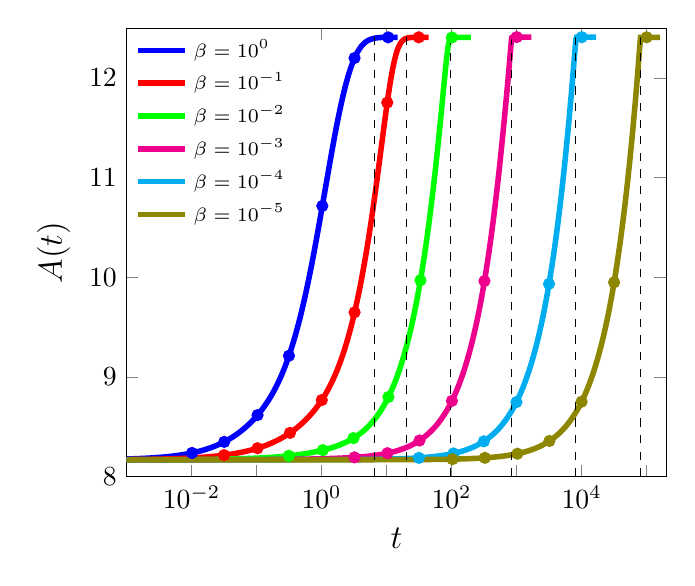
\begin{tikzpicture}[scale=1]

  \begin{axis}[
    xmin = 1e-3,
    xmax = 200000,
    xmode = log,
    xminorticks = false,
    xtick = {1e-3,1e-2,1e-1,1e0,1e1,1e2,1e3,1e4,1e5},
    xticklabels = {,$10^{-2}$,,$10^0$,,$10^2$,,$10^4$},
    ymin = 8,
    ymax = 12.5,
    xlabel = {\large $t$},
    ylabel = {\large ${A}(t)$},
    ylabel near ticks,
    legend entries = {$\beta=10^{0}$,
    $\beta = 10^{-1}$,
    $\beta = 10^{-2}$,
    $\beta = 10^{-3}$,
    $\beta = 10^{-4}$,
    $\beta = 10^{-5}$},
    legend cell align=left,
    legend style={draw=none,font=\scriptsize},
    legend style={at={(0.0,1.00)},anchor=north west}
  ]

\addplot[blue, line width=2pt] coordinates{
(9.4768e-04,8.1757e+00)
(9.8663e-04,8.1760e+00)
(1.0241e-03,8.1763e+00)
(1.0646e-03,8.1766e+00)
(1.1067e-03,8.1769e+00)
(1.1499e-03,8.1772e+00)
(1.1950e-03,8.1776e+00)
(1.2408e-03,8.1779e+00)
(1.2898e-03,8.1783e+00)
(1.3376e-03,8.1787e+00)
(1.3891e-03,8.1791e+00)
(1.4415e-03,8.1795e+00)
(1.4973e-03,8.1799e+00)
(1.5520e-03,8.1803e+00)
(1.6111e-03,8.1807e+00)
(1.6704e-03,8.1812e+00)
(1.7345e-03,8.1817e+00)
(1.7963e-03,8.1821e+00)
(1.8631e-03,8.1826e+00)
(1.9319e-03,8.1831e+00)
(2.0033e-03,8.1837e+00)
(2.0766e-03,8.1842e+00)
(2.1534e-03,8.1848e+00)
(2.2309e-03,8.1853e+00)
(2.3143e-03,8.1859e+00)
(2.3948e-03,8.1865e+00)
(2.4817e-03,8.1872e+00)
(2.5712e-03,8.1878e+00)
(2.6643e-03,8.1885e+00)
(2.7595e-03,8.1892e+00)
(2.8596e-03,8.1899e+00)
(2.9601e-03,8.1906e+00)
(3.0687e-03,8.1914e+00)
(3.1734e-03,8.1921e+00)
(3.2864e-03,8.1929e+00)
(3.4030e-03,8.1937e+00)
(3.5239e-03,8.1945e+00)
(3.6482e-03,8.1954e+00)
(3.7780e-03,8.1963e+00)
(3.9097e-03,8.1972e+00)
(4.0504e-03,8.1982e+00)
(4.1879e-03,8.1991e+00)
(4.3365e-03,8.2001e+00)
(4.4863e-03,8.2011e+00)
(4.6479e-03,8.2022e+00)
(4.8033e-03,8.2033e+00)
(4.9712e-03,8.2044e+00)
(5.1453e-03,8.2055e+00)
(5.3244e-03,8.2067e+00)
(5.5112e-03,8.2079e+00)
(5.7014e-03,8.2092e+00)
(5.9033e-03,8.2105e+00)
(6.1030e-03,8.2118e+00)
(6.3188e-03,8.2132e+00)
(6.5324e-03,8.2145e+00)
(6.7631e-03,8.2160e+00)
(6.9913e-03,8.2174e+00)
(7.2378e-03,8.2190e+00)
(7.4822e-03,8.2205e+00)
(7.7461e-03,8.2222e+00)
(8.0072e-03,8.2238e+00)
(8.2892e-03,8.2255e+00)
(8.5694e-03,8.2272e+00)
(8.8720e-03,8.2291e+00)
(9.1711e-03,8.2309e+00)
(9.4941e-03,8.2328e+00)
(9.8167e-03,8.2347e+00)
(1.0165e-02,8.2368e+00)
(1.0508e-02,8.2388e+00)
(1.0878e-02,8.2410e+00)
(1.1251e-02,8.2431e+00)
(1.1655e-02,8.2455e+00)
(1.2046e-02,8.2477e+00)
(1.2468e-02,8.2501e+00)
(1.2905e-02,8.2526e+00)
(1.3358e-02,8.2551e+00)
(1.3828e-02,8.2577e+00)
(1.4314e-02,8.2604e+00)
(1.4818e-02,8.2632e+00)
(1.5339e-02,8.2660e+00)
(1.5881e-02,8.2690e+00)
(1.6439e-02,8.2720e+00)
(1.7023e-02,8.2751e+00)
(1.7615e-02,8.2782e+00)
(1.8249e-02,8.2815e+00)
(1.8871e-02,8.2848e+00)
(1.9543e-02,8.2883e+00)
(2.0220e-02,8.2917e+00)
(2.0952e-02,8.2955e+00)
(2.1659e-02,8.2990e+00)
(2.2423e-02,8.3029e+00)
(2.3213e-02,8.3068e+00)
(2.4034e-02,8.3109e+00)
(2.4880e-02,8.3150e+00)
(2.5764e-02,8.3193e+00)
(2.6671e-02,8.3237e+00)
(2.7629e-02,8.3282e+00)
(2.8594e-02,8.3328e+00)
(2.9636e-02,8.3377e+00)
(3.0663e-02,8.3425e+00)
(3.1772e-02,8.3476e+00)
(3.2911e-02,8.3528e+00)
(3.4123e-02,8.3583e+00)
(3.5342e-02,8.3638e+00)
(3.6660e-02,8.3697e+00)
(3.7985e-02,8.3755e+00)
(3.9416e-02,8.3818e+00)
(4.0867e-02,8.3880e+00)
(4.2434e-02,8.3947e+00)
(4.4013e-02,8.4014e+00)
(4.5717e-02,8.4085e+00)
(4.7458e-02,8.4157e+00)
(4.9338e-02,8.4234e+00)
(5.1222e-02,8.4311e+00)
(5.3258e-02,8.4392e+00)
(5.5352e-02,8.4475e+00)
(5.7597e-02,8.4562e+00)
(5.9853e-02,8.4649e+00)
(6.2290e-02,8.4741e+00)
(6.4760e-02,8.4834e+00)
(6.7428e-02,8.4933e+00)
(7.0077e-02,8.5029e+00)
(7.2937e-02,8.5133e+00)
(7.5840e-02,8.5236e+00)
(7.8966e-02,8.5346e+00)
(8.2030e-02,8.5452e+00)
(8.5339e-02,8.5565e+00)
(8.8709e-02,8.5680e+00)
(9.2296e-02,8.5799e+00)
(9.5855e-02,8.5917e+00)
(9.9698e-02,8.6043e+00)
(1.0351e-01,8.6166e+00)
(1.0763e-01,8.6298e+00)
(1.1171e-01,8.6427e+00)
(1.1612e-01,8.6565e+00)
(1.2050e-01,8.6701e+00)
(1.2523e-01,8.6846e+00)
(1.2994e-01,8.6990e+00)
(1.3502e-01,8.7143e+00)
(1.4009e-01,8.7295e+00)
(1.4556e-01,8.7458e+00)
(1.5104e-01,8.7619e+00)
(1.5695e-01,8.7792e+00)
(1.6288e-01,8.7965e+00)
(1.6930e-01,8.8150e+00)
(1.7576e-01,8.8335e+00)
(1.8273e-01,8.8533e+00)
(1.8981e-01,8.8734e+00)
(1.9746e-01,8.8949e+00)
(2.0523e-01,8.9166e+00)
(2.1362e-01,8.9400e+00)
(2.2228e-01,8.9639e+00)
(2.3165e-01,8.9896e+00)
(2.4123e-01,9.0158e+00)
(2.5159e-01,9.0440e+00)
(2.6259e-01,9.0737e+00)
(2.7431e-01,9.1051e+00)
(2.8683e-01,9.1385e+00)
(3.0026e-01,9.1741e+00)
(3.1471e-01,9.2121e+00)
(3.3031e-01,9.2528e+00)
(3.4716e-01,9.2965e+00)
(3.6536e-01,9.3432e+00)
(3.8502e-01,9.3931e+00)
(4.0625e-01,9.4465e+00)
(4.2917e-01,9.5035e+00)
(4.5393e-01,9.5642e+00)
(4.8067e-01,9.6288e+00)
(5.0955e-01,9.6975e+00)
(5.4074e-01,9.7703e+00)
(5.7443e-01,9.8473e+00)
(6.1081e-01,9.9285e+00)
(6.5010e-01,1.0014e+01)
(6.9253e-01,1.0104e+01)
(7.3784e-01,1.0196e+01)
(7.8261e-01,1.0285e+01)
(8.3076e-01,1.0377e+01)
(8.7692e-01,1.0462e+01)
(9.2677e-01,1.0550e+01)
(9.7489e-01,1.0631e+01)
(1.0269e+00,1.0716e+01)
(1.0764e+00,1.0793e+01)
(1.1300e+00,1.0872e+01)
(1.1822e+00,1.0946e+01)
(1.2385e+00,1.1022e+01)
(1.2927e+00,1.1092e+01)
(1.3512e+00,1.1163e+01)
(1.4092e+00,1.1230e+01)
(1.4714e+00,1.1298e+01)
(1.5325e+00,1.1361e+01)
(1.5985e+00,1.1426e+01)
(1.6641e+00,1.1485e+01)
(1.7349e+00,1.1546e+01)
(1.8052e+00,1.1602e+01)
(1.8810e+00,1.1659e+01)
(1.9574e+00,1.1712e+01)
(2.0400e+00,1.1765e+01)
(2.1224e+00,1.1814e+01)
(2.2113e+00,1.1863e+01)
(2.3022e+00,1.1909e+01)
(2.4001e+00,1.1954e+01)
(2.4986e+00,1.1995e+01)
(2.6050e+00,1.2035e+01)
(2.7145e+00,1.2072e+01)
(2.8326e+00,1.2108e+01)
(2.9520e+00,1.2141e+01)
(3.0811e+00,1.2172e+01)
(3.2159e+00,1.2201e+01)
(3.3602e+00,1.2228e+01)
(3.5098e+00,1.2252e+01)
(3.6714e+00,1.2274e+01)
(3.8404e+00,1.2294e+01)
(4.0230e+00,1.2313e+01)
(4.2172e+00,1.2329e+01)
(4.4270e+00,1.2343e+01)
(4.6535e+00,1.2356e+01)
(4.8981e+00,1.2367e+01)
(5.1624e+00,1.2376e+01)
(5.4477e+00,1.2384e+01)
(5.7559e+00,1.2390e+01)
(6.0887e+00,1.2395e+01)
(6.4482e+00,1.2399e+01)
(6.8364e+00,1.2402e+01)
(7.2557e+00,1.2404e+01)
(7.7086e+00,1.2406e+01)
(8.1976e+00,1.2407e+01)
(8.7258e+00,1.2408e+01)
(9.2962e+00,1.2408e+01)
(9.9123e+00,1.2408e+01)
(1.0578e+01,1.2408e+01)
(1.1296e+01,1.2409e+01)
(1.2072e+01,1.2409e+01)
(1.2910e+01,1.2409e+01)
(1.3816e+01,1.2409e+01)
(1.4793e+01,1.2409e+01)
};

\addplot[red, line width=2pt] coordinates{
(8.9801e-04,8.1703e+00)
(9.6711e-04,8.1704e+00)
(1.0378e-03,8.1706e+00)
(1.1141e-03,8.1707e+00)
(1.1924e-03,8.1709e+00)
(1.2769e-03,8.1711e+00)
(1.3627e-03,8.1713e+00)
(1.4554e-03,8.1715e+00)
(1.5509e-03,8.1717e+00)
(1.6540e-03,8.1719e+00)
(1.7574e-03,8.1721e+00)
(1.8690e-03,8.1723e+00)
(1.9858e-03,8.1726e+00)
(2.1089e-03,8.1728e+00)
(2.2403e-03,8.1731e+00)
(2.3705e-03,8.1733e+00)
(2.5112e-03,8.1736e+00)
(2.6632e-03,8.1739e+00)
(2.8177e-03,8.1742e+00)
(2.9847e-03,8.1745e+00)
(3.1555e-03,8.1748e+00)
(3.3400e-03,8.1752e+00)
(3.5266e-03,8.1755e+00)
(3.7281e-03,8.1759e+00)
(3.9356e-03,8.1763e+00)
(4.1597e-03,8.1767e+00)
(4.3833e-03,8.1771e+00)
(4.6247e-03,8.1775e+00)
(4.8783e-03,8.1780e+00)
(5.1431e-03,8.1784e+00)
(5.4224e-03,8.1789e+00)
(5.7119e-03,8.1794e+00)
(6.0208e-03,8.1799e+00)
(6.3343e-03,8.1805e+00)
(6.6730e-03,8.1810e+00)
(7.0173e-03,8.1816e+00)
(7.3892e-03,8.1822e+00)
(7.7661e-03,8.1828e+00)
(8.1731e-03,8.1835e+00)
(8.5876e-03,8.1841e+00)
(9.0353e-03,8.1848e+00)
(9.4873e-03,8.1855e+00)
(9.9753e-03,8.1863e+00)
(1.0475e-02,8.1870e+00)
(1.1015e-02,8.1878e+00)
(1.1555e-02,8.1886e+00)
(1.2138e-02,8.1895e+00)
(1.2744e-02,8.1904e+00)
(1.3386e-02,8.1913e+00)
(1.4046e-02,8.1922e+00)
(1.4759e-02,8.1933e+00)
(1.5466e-02,8.1942e+00)
(1.6231e-02,8.1953e+00)
(1.7035e-02,8.1964e+00)
(1.7871e-02,8.1975e+00)
(1.8756e-02,8.1987e+00)
(1.9666e-02,8.1999e+00)
(2.0647e-02,8.2012e+00)
(2.1626e-02,8.2024e+00)
(2.2683e-02,8.2038e+00)
(2.3789e-02,8.2052e+00)
(2.4950e-02,8.2066e+00)
(2.6162e-02,8.2081e+00)
(2.7438e-02,8.2097e+00)
(2.8763e-02,8.2113e+00)
(3.0173e-02,8.2129e+00)
(3.1613e-02,8.2146e+00)
(3.3168e-02,8.2164e+00)
(3.4735e-02,8.2182e+00)
(3.6426e-02,8.2201e+00)
(3.8172e-02,8.2221e+00)
(4.0050e-02,8.2242e+00)
(4.1932e-02,8.2262e+00)
(4.3965e-02,8.2284e+00)
(4.6084e-02,8.2306e+00)
(4.8327e-02,8.2330e+00)
(5.0644e-02,8.2354e+00)
(5.3137e-02,8.2380e+00)
(5.5643e-02,8.2405e+00)
(5.8350e-02,8.2432e+00)
(6.1172e-02,8.2460e+00)
(6.4169e-02,8.2489e+00)
(6.7256e-02,8.2518e+00)
(7.0590e-02,8.2550e+00)
(7.3941e-02,8.2581e+00)
(7.7560e-02,8.2615e+00)
(8.1344e-02,8.2649e+00)
(8.5342e-02,8.2685e+00)
(8.9492e-02,8.2722e+00)
(9.3930e-02,8.2760e+00)
(9.8442e-02,8.2799e+00)
(1.0331e-01,8.2841e+00)
(1.0830e-01,8.2882e+00)
(1.1368e-01,8.2927e+00)
(1.1914e-01,8.2971e+00)
(1.2504e-01,8.3019e+00)
(1.3111e-01,8.3067e+00)
(1.3768e-01,8.3118e+00)
(1.4432e-01,8.3169e+00)
(1.5150e-01,8.3224e+00)
(1.5905e-01,8.3280e+00)
(1.6705e-01,8.3339e+00)
(1.7546e-01,8.3400e+00)
(1.8446e-01,8.3465e+00)
(1.9382e-01,8.3531e+00)
(2.0392e-01,8.3601e+00)
(2.1449e-01,8.3673e+00)
(2.2590e-01,8.3750e+00)
(2.3780e-01,8.3829e+00)
(2.5065e-01,8.3912e+00)
(2.6410e-01,8.3999e+00)
(2.7863e-01,8.4090e+00)
(2.9359e-01,8.4183e+00)
(3.0974e-01,8.4281e+00)
(3.2647e-01,8.4381e+00)
(3.4453e-01,8.4487e+00)
(3.6267e-01,8.4592e+00)
(3.8226e-01,8.4703e+00)
(4.0247e-01,8.4815e+00)
(4.2405e-01,8.4934e+00)
(4.4580e-01,8.5051e+00)
(4.6929e-01,8.5175e+00)
(4.9301e-01,8.5299e+00)
(5.1862e-01,8.5430e+00)
(5.4454e-01,8.5560e+00)
(5.7254e-01,8.5699e+00)
(6.0108e-01,8.5839e+00)
(6.3190e-01,8.5988e+00)
(6.6353e-01,8.6138e+00)
(6.9769e-01,8.6298e+00)
(7.3322e-01,8.6462e+00)
(7.7158e-01,8.6638e+00)
(8.1191e-01,8.6820e+00)
(8.5546e-01,8.7014e+00)
(9.0232e-01,8.7221e+00)
(9.5293e-01,8.7442e+00)
(1.0076e+00,8.7678e+00)
(1.0666e+00,8.7930e+00)
(1.1304e+00,8.8201e+00)
(1.1992e+00,8.8491e+00)
(1.2736e+00,8.8801e+00)
(1.3539e+00,8.9134e+00)
(1.4406e+00,8.9491e+00)
(1.5343e+00,8.9874e+00)
(1.6355e+00,9.0285e+00)
(1.7447e+00,9.0726e+00)
(1.8627e+00,9.1201e+00)
(1.9901e+00,9.1710e+00)
(2.1278e+00,9.2257e+00)
(2.2764e+00,9.2844e+00)
(2.4370e+00,9.3474e+00)
(2.6103e+00,9.4150e+00)
(2.7976e+00,9.4875e+00)
(2.9998e+00,9.5652e+00)
(3.2182e+00,9.6483e+00)
(3.4541e+00,9.7372e+00)
(3.7088e+00,9.8322e+00)
(3.9840e+00,9.9336e+00)
(4.2811e+00,1.0041e+01)
(4.6020e+00,1.0156e+01)
(4.9486e+00,1.0278e+01)
(5.3229e+00,1.0406e+01)
(5.6770e+00,1.0525e+01)
(5.9957e+00,1.0630e+01)
(6.3399e+00,1.0740e+01)
(6.7116e+00,1.0856e+01)
(7.0771e+00,1.0967e+01)
(7.4393e+00,1.1072e+01)
(7.7963e+00,1.1173e+01)
(8.1517e+00,1.1270e+01)
(8.5014e+00,1.1361e+01)
(8.8524e+00,1.1449e+01)
(9.1955e+00,1.1530e+01)
(9.5460e+00,1.1610e+01)
(9.8822e+00,1.1682e+01)
(1.0239e+01,1.1754e+01)
(1.0565e+01,1.1816e+01)
(1.0917e+01,1.1878e+01)
(1.1259e+01,1.1935e+01)
(1.1625e+01,1.1990e+01)
(1.1965e+01,1.2037e+01)
(1.2333e+01,1.2084e+01)
(1.2707e+01,1.2126e+01)
(1.3095e+01,1.2166e+01)
(1.3492e+01,1.2201e+01)
(1.3914e+01,1.2234e+01)
(1.4341e+01,1.2263e+01)
(1.4803e+01,1.2289e+01)
(1.5291e+01,1.2312e+01)
(1.5819e+01,1.2332e+01)
(1.6387e+01,1.2350e+01)
(1.7001e+01,1.2364e+01)
(1.7664e+01,1.2376e+01)
(1.8381e+01,1.2385e+01)
(1.9154e+01,1.2393e+01)
(1.9989e+01,1.2398e+01)
(2.0891e+01,1.2402e+01)
(2.1866e+01,1.2404e+01)
(2.2918e+01,1.2406e+01)
(2.4054e+01,1.2407e+01)
(2.5281e+01,1.2408e+01)
(2.6607e+01,1.2408e+01)
(2.8038e+01,1.2409e+01)
(2.9584e+01,1.2409e+01)
(3.1254e+01,1.2409e+01)
(3.3057e+01,1.2409e+01)
(3.5005e+01,1.2409e+01)
(3.7108e+01,1.2409e+01)
(3.9380e+01,1.2409e+01)
(4.1833e+01,1.2409e+01)
(4.4483e+01,1.2409e+01)
};

\addplot[green, line width=2pt] coordinates{
(8.4580e-04,8.1684e+00)
(9.4755e-04,8.1684e+00)
(1.0574e-03,8.1684e+00)
(1.1761e-03,8.1685e+00)
(1.3043e-03,8.1685e+00)
(1.4427e-03,8.1685e+00)
(1.5922e-03,8.1686e+00)
(1.7537e-03,8.1686e+00)
(1.9281e-03,8.1687e+00)
(2.1164e-03,8.1687e+00)
(2.3198e-03,8.1688e+00)
(2.5395e-03,8.1688e+00)
(2.7768e-03,8.1689e+00)
(3.0330e-03,8.1690e+00)
(3.3097e-03,8.1690e+00)
(3.6086e-03,8.1691e+00)
(3.9314e-03,8.1692e+00)
(4.2800e-03,8.1693e+00)
(4.6564e-03,8.1694e+00)
(5.0631e-03,8.1695e+00)
(5.5022e-03,8.1696e+00)
(5.9737e-03,8.1697e+00)
(6.4672e-03,8.1698e+00)
(7.0003e-03,8.1699e+00)
(7.5566e-03,8.1700e+00)
(8.1573e-03,8.1702e+00)
(8.7843e-03,8.1703e+00)
(9.4615e-03,8.1704e+00)
(1.0165e-02,8.1706e+00)
(1.0925e-02,8.1707e+00)
(1.1717e-02,8.1709e+00)
(1.2573e-02,8.1711e+00)
(1.3457e-02,8.1713e+00)
(1.4411e-02,8.1715e+00)
(1.5409e-02,8.1717e+00)
(1.6487e-02,8.1719e+00)
(1.7591e-02,8.1721e+00)
(1.8782e-02,8.1723e+00)
(2.0041e-02,8.1725e+00)
(2.1375e-02,8.1728e+00)
(2.2780e-02,8.1730e+00)
(2.4277e-02,8.1733e+00)
(2.5838e-02,8.1736e+00)
(2.7524e-02,8.1739e+00)
(2.9244e-02,8.1742e+00)
(3.1103e-02,8.1745e+00)
(3.3064e-02,8.1748e+00)
(3.5141e-02,8.1752e+00)
(3.7327e-02,8.1755e+00)
(3.9651e-02,8.1759e+00)
(4.2083e-02,8.1763e+00)
(4.4693e-02,8.1767e+00)
(4.7379e-02,8.1771e+00)
(5.0279e-02,8.1776e+00)
(5.3296e-02,8.1781e+00)
(5.6554e-02,8.1785e+00)
(5.9884e-02,8.1790e+00)
(6.3482e-02,8.1796e+00)
(6.7262e-02,8.1801e+00)
(7.1292e-02,8.1807e+00)
(7.5489e-02,8.1813e+00)
(8.0022e-02,8.1819e+00)
(8.4654e-02,8.1825e+00)
(8.9657e-02,8.1832e+00)
(9.4927e-02,8.1839e+00)
(1.0053e-01,8.1846e+00)
(1.0640e-01,8.1853e+00)
(1.1270e-01,8.1861e+00)
(1.1920e-01,8.1869e+00)
(1.2623e-01,8.1878e+00)
(1.3354e-01,8.1887e+00)
(1.4144e-01,8.1896e+00)
(1.4957e-01,8.1906e+00)
(1.5834e-01,8.1916e+00)
(1.6755e-01,8.1926e+00)
(1.7743e-01,8.1938e+00)
(1.8767e-01,8.1949e+00)
(1.9873e-01,8.1961e+00)
(2.1022e-01,8.1973e+00)
(2.2263e-01,8.1986e+00)
(2.3551e-01,8.2000e+00)
(2.4941e-01,8.2014e+00)
(2.6393e-01,8.2028e+00)
(2.7962e-01,8.2044e+00)
(2.9597e-01,8.2060e+00)
(3.1362e-01,8.2077e+00)
(3.3229e-01,8.2094e+00)
(3.5244e-01,8.2113e+00)
(3.7360e-01,8.2133e+00)
(3.9644e-01,8.2153e+00)
(4.2098e-01,8.2175e+00)
(4.4715e-01,8.2198e+00)
(4.7538e-01,8.2222e+00)
(5.0531e-01,8.2247e+00)
(5.3763e-01,8.2273e+00)
(5.7179e-01,8.2301e+00)
(6.0869e-01,8.2330e+00)
(6.4706e-01,8.2360e+00)
(6.8851e-01,8.2392e+00)
(7.3155e-01,8.2424e+00)
(7.7803e-01,8.2459e+00)
(8.2549e-01,8.2493e+00)
(8.7674e-01,8.2530e+00)
(9.3002e-01,8.2567e+00)
(9.8749e-01,8.2606e+00)
(1.0462e+00,8.2646e+00)
(1.1096e+00,8.2688e+00)
(1.1771e+00,8.2732e+00)
(1.2488e+00,8.2779e+00)
(1.3262e+00,8.2828e+00)
(1.4086e+00,8.2879e+00)
(1.4976e+00,8.2934e+00)
(1.5937e+00,8.2992e+00)
(1.6976e+00,8.3055e+00)
(1.8097e+00,8.3121e+00)
(1.9308e+00,8.3192e+00)
(2.0616e+00,8.3268e+00)
(2.2028e+00,8.3350e+00)
(2.3554e+00,8.3437e+00)
(2.5202e+00,8.3530e+00)
(2.6981e+00,8.3630e+00)
(2.8903e+00,8.3738e+00)
(3.0978e+00,8.3854e+00)
(3.3220e+00,8.3979e+00)
(3.5641e+00,8.4113e+00)
(3.8255e+00,8.4257e+00)
(4.1079e+00,8.4413e+00)
(4.4129e+00,8.4581e+00)
(4.7422e+00,8.4762e+00)
(5.0979e+00,8.4957e+00)
(5.4821e+00,8.5168e+00)
(5.8970e+00,8.5395e+00)
(6.3451e+00,8.5639e+00)
(6.8290e+00,8.5903e+00)
(7.3517e+00,8.6188e+00)
(7.9161e+00,8.6495e+00)
(8.5258e+00,8.6826e+00)
(9.1842e+00,8.7183e+00)
(9.8952e+00,8.7567e+00)
(1.0663e+01,8.7981e+00)
(1.1493e+01,8.8428e+00)
(1.2388e+01,8.8908e+00)
(1.3356e+01,8.9426e+00)
(1.4400e+01,8.9984e+00)
(1.5529e+01,9.0584e+00)
(1.6747e+01,9.1230e+00)
(1.8064e+01,9.1924e+00)
(1.9485e+01,9.2671e+00)
(2.1020e+01,9.3475e+00)
(2.2678e+01,9.4338e+00)
(2.4469e+01,9.5265e+00)
(2.6402e+01,9.6260e+00)
(2.8491e+01,9.7328e+00)
(3.0747e+01,9.8473e+00)
(3.3183e+01,9.9701e+00)
(3.5814e+01,1.0101e+01)
(3.8655e+01,1.0242e+01)
(4.1724e+01,1.0392e+01)
(4.5038e+01,1.0552e+01)
(4.8617e+01,1.0723e+01)
(5.2483e+01,1.0904e+01)
(5.6658e+01,1.1096e+01)
(5.9881e+01,1.1242e+01)
(6.2782e+01,1.1371e+01)
(6.5915e+01,1.1507e+01)
(6.8271e+01,1.1608e+01)
(7.0392e+01,1.1697e+01)
(7.2683e+01,1.1791e+01)
(7.4546e+01,1.1866e+01)
(7.6222e+01,1.1931e+01)
(7.8032e+01,1.1999e+01)
(7.9448e+01,1.2051e+01)
(8.0722e+01,1.2095e+01)
(8.2097e+01,1.2142e+01)
(8.3366e+01,1.2182e+01)
(8.4508e+01,1.2216e+01)
(8.5741e+01,1.2251e+01)
(8.6817e+01,1.2279e+01)
(8.7785e+01,1.2301e+01)
(8.8830e+01,1.2323e+01)
(8.9960e+01,1.2343e+01)
(9.1041e+01,1.2360e+01)
(9.2209e+01,1.2374e+01)
(9.3410e+01,1.2385e+01)
(9.4707e+01,1.2393e+01)
(9.6108e+01,1.2399e+01)
(9.7620e+01,1.2403e+01)
(9.9254e+01,1.2406e+01)
(1.0102e+02,1.2407e+01)
(1.0292e+02,1.2408e+01)
(1.0498e+02,1.2409e+01)
(1.0720e+02,1.2409e+01)
(1.0960e+02,1.2409e+01)
(1.1220e+02,1.2409e+01)
(1.1500e+02,1.2409e+01)
(1.1802e+02,1.2409e+01)
(1.2129e+02,1.2409e+01)
(1.2481e+02,1.2409e+01)
(1.2862e+02,1.2409e+01)
(1.3274e+02,1.2409e+01)
(1.3718e+02,1.2409e+01)
(1.4198e+02,1.2409e+01)
(1.4716e+02,1.2409e+01)
(1.5276e+02,1.2409e+01)
(1.5880e+02,1.2409e+01)
(1.6533e+02,1.2409e+01)
(1.7238e+02,1.2409e+01)
(1.8000e+02,1.2409e+01)
(1.8822e+02,1.2409e+01)
(1.9710e+02,1.2409e+01)
};

\addplot[magenta, line width=2pt] coordinates{
(7.8511e-04,8.1682e+00)
(9.0052e-04,8.1682e+00)
(1.0252e-03,8.1682e+00)
(1.1598e-03,8.1682e+00)
(1.3052e-03,8.1682e+00)
(1.4622e-03,8.1682e+00)
(1.6318e-03,8.1682e+00)
(1.8149e-03,8.1682e+00)
(2.0127e-03,8.1682e+00)
(2.2263e-03,8.1682e+00)
(2.4570e-03,8.1682e+00)
(2.7062e-03,8.1682e+00)
(2.9753e-03,8.1682e+00)
(3.2659e-03,8.1682e+00)
(3.5798e-03,8.1682e+00)
(3.9188e-03,8.1682e+00)
(4.2849e-03,8.1683e+00)
(4.6803e-03,8.1683e+00)
(5.1073e-03,8.1683e+00)
(5.5685e-03,8.1683e+00)
(6.0666e-03,8.1683e+00)
(6.6045e-03,8.1683e+00)
(7.1855e-03,8.1683e+00)
(7.8129e-03,8.1683e+00)
(8.4905e-03,8.1684e+00)
(9.2224e-03,8.1684e+00)
(9.9991e-03,8.1684e+00)
(1.0827e-02,8.1684e+00)
(1.1702e-02,8.1684e+00)
(1.2641e-02,8.1684e+00)
(1.3621e-02,8.1685e+00)
(1.4679e-02,8.1685e+00)
(1.5779e-02,8.1685e+00)
(1.6968e-02,8.1685e+00)
(1.8208e-02,8.1686e+00)
(1.9547e-02,8.1686e+00)
(2.0933e-02,8.1686e+00)
(2.2430e-02,8.1686e+00)
(2.3996e-02,8.1687e+00)
(2.5687e-02,8.1687e+00)
(2.7422e-02,8.1687e+00)
(2.9295e-02,8.1688e+00)
(3.1276e-02,8.1688e+00)
(3.3376e-02,8.1689e+00)
(3.5593e-02,8.1689e+00)
(3.7949e-02,8.1689e+00)
(4.0425e-02,8.1690e+00)
(4.3074e-02,8.1690e+00)
(4.5826e-02,8.1691e+00)
(4.8797e-02,8.1691e+00)
(5.1865e-02,8.1692e+00)
(5.5178e-02,8.1692e+00)
(5.8630e-02,8.1693e+00)
(6.2358e-02,8.1693e+00)
(6.6187e-02,8.1694e+00)
(7.0322e-02,8.1695e+00)
(7.4666e-02,8.1695e+00)
(7.9318e-02,8.1696e+00)
(8.4141e-02,8.1697e+00)
(8.9350e-02,8.1697e+00)
(9.4748e-02,8.1698e+00)
(1.0058e-01,8.1699e+00)
(1.0663e-01,8.1700e+00)
(1.1316e-01,8.1701e+00)
(1.1994e-01,8.1702e+00)
(1.2725e-01,8.1703e+00)
(1.3486e-01,8.1703e+00)
(1.4308e-01,8.1705e+00)
(1.5159e-01,8.1706e+00)
(1.6079e-01,8.1707e+00)
(1.7039e-01,8.1708e+00)
(1.8076e-01,8.1709e+00)
(1.9148e-01,8.1710e+00)
(2.0304e-01,8.1712e+00)
(2.1521e-01,8.1713e+00)
(2.2829e-01,8.1715e+00)
(2.4187e-01,8.1716e+00)
(2.5654e-01,8.1718e+00)
(2.7191e-01,8.1719e+00)
(2.8850e-01,8.1721e+00)
(3.0579e-01,8.1723e+00)
(3.2446e-01,8.1725e+00)
(3.4425e-01,8.1727e+00)
(3.6555e-01,8.1729e+00)
(3.8802e-01,8.1731e+00)
(4.1229e-01,8.1734e+00)
(4.3823e-01,8.1736e+00)
(4.6618e-01,8.1739e+00)
(4.9600e-01,8.1741e+00)
(5.2821e-01,8.1744e+00)
(5.6259e-01,8.1747e+00)
(5.9972e-01,8.1751e+00)
(6.3901e-01,8.1754e+00)
(6.8145e-01,8.1758e+00)
(7.2600e-01,8.1761e+00)
(7.7412e-01,8.1765e+00)
(8.2397e-01,8.1769e+00)
(8.7782e-01,8.1773e+00)
(9.3363e-01,8.1778e+00)
(9.9391e-01,8.1782e+00)
(1.0560e+00,8.1787e+00)
(1.1231e+00,8.1792e+00)
(1.1935e+00,8.1797e+00)
(1.2696e+00,8.1802e+00)
(1.3493e+00,8.1807e+00)
(1.4353e+00,8.1813e+00)
(1.5282e+00,8.1819e+00)
(1.6286e+00,8.1826e+00)
(1.7370e+00,8.1833e+00)
(1.8540e+00,8.1841e+00)
(1.9805e+00,8.1849e+00)
(2.1170e+00,8.1857e+00)
(2.2645e+00,8.1866e+00)
(2.4237e+00,8.1876e+00)
(2.5957e+00,8.1887e+00)
(2.7815e+00,8.1898e+00)
(2.9821e+00,8.1910e+00)
(3.1988e+00,8.1923e+00)
(3.4328e+00,8.1937e+00)
(3.6855e+00,8.1952e+00)
(3.9584e+00,8.1968e+00)
(4.2532e+00,8.1986e+00)
(4.5716e+00,8.2004e+00)
(4.9154e+00,8.2025e+00)
(5.2868e+00,8.2046e+00)
(5.6878e+00,8.2070e+00)
(6.1209e+00,8.2096e+00)
(6.5887e+00,8.2123e+00)
(7.0939e+00,8.2153e+00)
(7.6395e+00,8.2185e+00)
(8.2288e+00,8.2219e+00)
(8.8652e+00,8.2257e+00)
(9.5525e+00,8.2297e+00)
(1.0295e+01,8.2341e+00)
(1.1096e+01,8.2388e+00)
(1.1962e+01,8.2439e+00)
(1.2897e+01,8.2494e+00)
(1.3907e+01,8.2553e+00)
(1.4998e+01,8.2617e+00)
(1.6176e+01,8.2686e+00)
(1.7448e+01,8.2760e+00)
(1.8822e+01,8.2841e+00)
(2.0306e+01,8.2928e+00)
(2.1908e+01,8.3021e+00)
(2.3639e+01,8.3123e+00)
(2.5509e+01,8.3232e+00)
(2.7527e+01,8.3350e+00)
(2.9708e+01,8.3477e+00)
(3.2062e+01,8.3614e+00)
(3.4605e+01,8.3763e+00)
(3.7352e+01,8.3922e+00)
(4.0318e+01,8.4095e+00)
(4.3522e+01,8.4281e+00)
(4.6982e+01,8.4482e+00)
(5.0718e+01,8.4698e+00)
(5.4754e+01,8.4932e+00)
(5.9112e+01,8.5184e+00)
(6.3819e+01,8.5455e+00)
(6.8903e+01,8.5748e+00)
(7.4393e+01,8.6064e+00)
(8.0323e+01,8.6404e+00)
(8.6727e+01,8.6771e+00)
(9.3643e+01,8.7167e+00)
(1.0111e+02,8.7592e+00)
(1.0918e+02,8.8051e+00)
(1.1789e+02,8.8545e+00)
(1.2730e+02,8.9077e+00)
(1.3746e+02,8.9650e+00)
(1.4844e+02,9.0266e+00)
(1.6029e+02,9.0930e+00)
(1.7309e+02,9.1643e+00)
(1.8692e+02,9.2410e+00)
(2.0185e+02,9.3234e+00)
(2.1798e+02,9.4120e+00)
(2.3539e+02,9.5071e+00)
(2.5420e+02,9.6093e+00)
(2.7452e+02,9.7189e+00)
(2.9646e+02,9.8364e+00)
(3.2015e+02,9.9624e+00)
(3.4574e+02,1.0097e+01)
(3.7338e+02,1.0242e+01)
(4.0323e+02,1.0396e+01)
(4.3546e+02,1.0561e+01)
(4.7028e+02,1.0737e+01)
(5.0788e+02,1.0924e+01)
(5.4849e+02,1.1122e+01)
(5.9234e+02,1.1332e+01)
(6.3971e+02,1.1553e+01)
(6.9087e+02,1.1783e+01)
(7.3860e+02,1.1988e+01)
(7.6471e+02,1.2103e+01)
(7.8821e+02,1.2203e+01)
(7.9978e+02,1.2253e+01)
(8.1019e+02,1.2297e+01)
(8.1786e+02,1.2328e+01)
(8.2476e+02,1.2355e+01)
(8.2894e+02,1.2370e+01)
(8.3270e+02,1.2383e+01)
(8.3676e+02,1.2394e+01)
(8.4008e+02,1.2402e+01)
(8.4307e+02,1.2406e+01)
(8.4630e+02,1.2409e+01)
(8.4979e+02,1.2410e+01)
(8.5355e+02,1.2410e+01)
(8.5762e+02,1.2411e+01)
(8.6201e+02,1.2411e+01)
(8.6676e+02,1.2411e+01)
(8.7188e+02,1.2411e+01)
(8.7741e+02,1.2411e+01)
(8.8339e+02,1.2411e+01)
(8.8984e+02,1.2411e+01)
(8.9681e+02,1.2411e+01)
(9.0434e+02,1.2411e+01)
(9.1247e+02,1.2411e+01)
(9.2125e+02,1.2411e+01)
(9.3074e+02,1.2411e+01)
(9.4098e+02,1.2411e+01)
(9.5204e+02,1.2411e+01)
(9.6399e+02,1.2411e+01)
(9.7689e+02,1.2411e+01)
(9.9082e+02,1.2411e+01)
(1.0059e+03,1.2411e+01)
(1.0221e+03,1.2411e+01)
(1.0397e+03,1.2411e+01)
(1.0586e+03,1.2411e+01)
(1.0791e+03,1.2411e+01)
(1.1012e+03,1.2411e+01)
(1.1251e+03,1.2411e+01)
(1.1509e+03,1.2411e+01)
(1.1787e+03,1.2411e+01)
(1.2088e+03,1.2411e+01)
(1.2413e+03,1.2411e+01)
(1.2764e+03,1.2411e+01)
(1.3143e+03,1.2411e+01)
(1.3552e+03,1.2411e+01)
(1.3994e+03,1.2411e+01)
(1.4472e+03,1.2411e+01)
(1.4987e+03,1.2411e+01)
(1.5544e+03,1.2411e+01)
(1.6145e+03,1.2411e+01)
(1.6795e+03,1.2411e+01)
};

\addplot[cyan, line width=2pt] coordinates{
(8.1786e-04,8.1681e+00)
(9.4671e-04,8.1681e+00)
(1.0859e-03,8.1681e+00)
(1.2362e-03,8.1681e+00)
(1.3985e-03,8.1681e+00)
(1.5738e-03,8.1681e+00)
(1.7632e-03,8.1681e+00)
(1.9676e-03,8.1681e+00)
(2.1885e-03,8.1681e+00)
(2.4270e-03,8.1681e+00)
(2.6846e-03,8.1681e+00)
(2.9628e-03,8.1681e+00)
(3.2632e-03,8.1681e+00)
(3.5877e-03,8.1682e+00)
(3.9381e-03,8.1682e+00)
(4.3166e-03,8.1682e+00)
(4.7254e-03,8.1682e+00)
(5.1669e-03,8.1682e+00)
(5.6436e-03,8.1682e+00)
(6.1586e-03,8.1682e+00)
(6.7147e-03,8.1682e+00)
(7.3153e-03,8.1682e+00)
(7.9639e-03,8.1682e+00)
(8.6645e-03,8.1682e+00)
(9.4210e-03,8.1682e+00)
(1.0214e-02,8.1682e+00)
(1.1071e-02,8.1682e+00)
(1.1964e-02,8.1682e+00)
(1.2929e-02,8.1682e+00)
(1.3939e-02,8.1682e+00)
(1.5030e-02,8.1682e+00)
(1.6161e-02,8.1682e+00)
(1.7381e-02,8.1682e+00)
(1.8664e-02,8.1682e+00)
(2.0045e-02,8.1682e+00)
(2.1470e-02,8.1682e+00)
(2.3010e-02,8.1682e+00)
(2.4627e-02,8.1682e+00)
(2.6364e-02,8.1682e+00)
(2.8162e-02,8.1682e+00)
(3.0104e-02,8.1682e+00)
(3.2128e-02,8.1682e+00)
(3.4315e-02,8.1682e+00)
(3.6564e-02,8.1682e+00)
(3.8994e-02,8.1682e+00)
(4.1545e-02,8.1682e+00)
(4.4281e-02,8.1682e+00)
(4.7112e-02,8.1682e+00)
(5.0169e-02,8.1682e+00)
(5.3346e-02,8.1682e+00)
(5.6777e-02,8.1683e+00)
(6.0318e-02,8.1683e+00)
(6.4142e-02,8.1683e+00)
(6.8131e-02,8.1683e+00)
(7.2439e-02,8.1683e+00)
(7.6859e-02,8.1683e+00)
(8.1633e-02,8.1683e+00)
(8.6663e-02,8.1683e+00)
(9.2024e-02,8.1683e+00)
(9.7633e-02,8.1683e+00)
(1.0369e-01,8.1683e+00)
(1.0989e-01,8.1683e+00)
(1.1660e-01,8.1683e+00)
(1.2368e-01,8.1683e+00)
(1.3121e-01,8.1684e+00)
(1.3915e-01,8.1684e+00)
(1.4762e-01,8.1684e+00)
(1.5649e-01,8.1684e+00)
(1.6606e-01,8.1684e+00)
(1.7592e-01,8.1684e+00)
(1.8656e-01,8.1684e+00)
(1.9782e-01,8.1684e+00)
(2.0981e-01,8.1685e+00)
(2.2242e-01,8.1685e+00)
(2.3598e-01,8.1685e+00)
(2.5007e-01,8.1685e+00)
(2.6529e-01,8.1685e+00)
(2.8125e-01,8.1685e+00)
(2.9849e-01,8.1685e+00)
(3.1645e-01,8.1686e+00)
(3.3585e-01,8.1686e+00)
(3.5648e-01,8.1686e+00)
(3.7861e-01,8.1686e+00)
(4.0213e-01,8.1687e+00)
(4.2752e-01,8.1687e+00)
(4.5449e-01,8.1687e+00)
(4.8362e-01,8.1687e+00)
(5.1489e-01,8.1688e+00)
(5.4849e-01,8.1688e+00)
(5.8452e-01,8.1688e+00)
(6.2316e-01,8.1688e+00)
(6.6440e-01,8.1689e+00)
(7.0851e-01,8.1689e+00)
(7.5520e-01,8.1690e+00)
(8.0510e-01,8.1690e+00)
(8.5737e-01,8.1690e+00)
(9.1358e-01,8.1691e+00)
(9.7150e-01,8.1691e+00)
(1.0341e+00,8.1692e+00)
(1.0993e+00,8.1692e+00)
(1.1697e+00,8.1693e+00)
(1.2428e+00,8.1693e+00)
(1.3218e+00,8.1694e+00)
(1.4067e+00,8.1694e+00)
(1.4977e+00,8.1695e+00)
(1.5960e+00,8.1696e+00)
(1.7022e+00,8.1696e+00)
(1.8169e+00,8.1697e+00)
(1.9407e+00,8.1698e+00)
(2.0744e+00,8.1699e+00)
(2.2189e+00,8.1699e+00)
(2.3749e+00,8.1700e+00)
(2.5434e+00,8.1701e+00)
(2.7253e+00,8.1703e+00)
(2.9218e+00,8.1704e+00)
(3.1341e+00,8.1705e+00)
(3.3633e+00,8.1706e+00)
(3.6108e+00,8.1708e+00)
(3.8782e+00,8.1710e+00)
(4.1669e+00,8.1711e+00)
(4.4787e+00,8.1713e+00)
(4.8155e+00,8.1715e+00)
(5.1793e+00,8.1717e+00)
(5.5721e+00,8.1720e+00)
(5.9963e+00,8.1722e+00)
(6.4545e+00,8.1725e+00)
(6.9494e+00,8.1728e+00)
(7.4838e+00,8.1731e+00)
(8.0610e+00,8.1734e+00)
(8.6844e+00,8.1738e+00)
(9.3576e+00,8.1742e+00)
(1.0085e+01,8.1746e+00)
(1.0870e+01,8.1751e+00)
(1.1718e+01,8.1756e+00)
(1.2634e+01,8.1761e+00)
(1.3623e+01,8.1767e+00)
(1.4692e+01,8.1774e+00)
(1.5845e+01,8.1781e+00)
(1.7091e+01,8.1788e+00)
(1.8437e+01,8.1796e+00)
(1.9891e+01,8.1804e+00)
(2.1460e+01,8.1814e+00)
(2.3156e+01,8.1824e+00)
(2.4987e+01,8.1835e+00)
(2.6964e+01,8.1846e+00)
(2.9100e+01,8.1859e+00)
(3.1406e+01,8.1873e+00)
(3.3897e+01,8.1887e+00)
(3.6587e+01,8.1903e+00)
(3.9493e+01,8.1921e+00)
(4.2631e+01,8.1939e+00)
(4.6020e+01,8.1959e+00)
(4.9680e+01,8.1981e+00)
(5.3633e+01,8.2004e+00)
(5.7902e+01,8.2030e+00)
(6.2513e+01,8.2057e+00)
(6.7492e+01,8.2086e+00)
(7.2870e+01,8.2118e+00)
(7.8678e+01,8.2153e+00)
(8.4951e+01,8.2190e+00)
(9.1725e+01,8.2230e+00)
(9.9042e+01,8.2273e+00)
(1.0694e+02,8.2320e+00)
(1.1548e+02,8.2370e+00)
(1.2469e+02,8.2424e+00)
(1.3465e+02,8.2483e+00)
(1.4540e+02,8.2547e+00)
(1.5701e+02,8.2615e+00)
(1.6955e+02,8.2689e+00)
(1.8309e+02,8.2769e+00)
(1.9772e+02,8.2855e+00)
(2.1351e+02,8.2948e+00)
(2.3057e+02,8.3048e+00)
(2.4900e+02,8.3157e+00)
(2.6889e+02,8.3274e+00)
(2.9038e+02,8.3400e+00)
(3.1359e+02,8.3536e+00)
(3.3866e+02,8.3683e+00)
(3.6573e+02,8.3842e+00)
(3.9497e+02,8.4013e+00)
(4.2654e+02,8.4197e+00)
(4.6064e+02,8.4396e+00)
(4.9747e+02,8.4611e+00)
(5.3725e+02,8.4842e+00)
(5.8021e+02,8.5092e+00)
(6.2660e+02,8.5361e+00)
(6.7671e+02,8.5651e+00)
(7.3083e+02,8.5963e+00)
(7.8927e+02,8.6300e+00)
(8.5239e+02,8.6663e+00)
(9.2056e+02,8.7054e+00)
(9.9418e+02,8.7475e+00)
(1.0737e+03,8.7928e+00)
(1.1596e+03,8.8415e+00)
(1.2523e+03,8.8940e+00)
(1.3523e+03,8.9503e+00)
(1.4523e+03,9.0064e+00)
(1.5523e+03,9.0623e+00)
(1.6523e+03,9.1181e+00)
(1.7523e+03,9.1736e+00)
(1.8523e+03,9.2290e+00)
(1.9523e+03,9.2843e+00)
(2.0523e+03,9.3393e+00)
(2.1523e+03,9.3942e+00)
(2.2523e+03,9.4489e+00)
(2.3523e+03,9.5035e+00)
(2.4523e+03,9.5579e+00)
(2.5523e+03,9.6121e+00)
(2.6523e+03,9.6662e+00)
(2.7523e+03,9.7201e+00)
(2.8523e+03,9.7738e+00)
(2.9523e+03,9.8274e+00)
(3.0523e+03,9.8808e+00)
(3.1523e+03,9.9341e+00)
(3.2523e+03,9.9872e+00)
(3.3523e+03,1.0040e+01)
(3.4523e+03,1.0093e+01)
(3.5523e+03,1.0146e+01)
(3.6523e+03,1.0198e+01)
(3.7523e+03,1.0250e+01)
(3.8523e+03,1.0303e+01)
(3.9523e+03,1.0355e+01)
(4.0523e+03,1.0407e+01)
(4.1523e+03,1.0458e+01)
(4.2523e+03,1.0510e+01)
(4.3523e+03,1.0561e+01)
(4.4523e+03,1.0613e+01)
(4.5523e+03,1.0664e+01)
(4.6523e+03,1.0715e+01)
(4.7523e+03,1.0766e+01)
(4.8523e+03,1.0817e+01)
(4.9523e+03,1.0867e+01)
(5.0523e+03,1.0918e+01)
(5.1523e+03,1.0968e+01)
(5.2523e+03,1.1018e+01)
(5.3523e+03,1.1068e+01)
(5.4523e+03,1.1118e+01)
(5.5523e+03,1.1167e+01)
(5.6523e+03,1.1217e+01)
(5.7523e+03,1.1266e+01)
(5.8523e+03,1.1316e+01)
(5.9523e+03,1.1365e+01)
(6.0523e+03,1.1414e+01)
(6.1523e+03,1.1463e+01)
(6.2523e+03,1.1511e+01)
(6.3523e+03,1.1560e+01)
(6.4523e+03,1.1608e+01)
(6.5523e+03,1.1656e+01)
(6.6523e+03,1.1704e+01)
(6.7523e+03,1.1752e+01)
(6.8523e+03,1.1799e+01)
(6.9523e+03,1.1847e+01)
(7.0523e+03,1.1894e+01)
(7.1523e+03,1.1940e+01)
(7.2523e+03,1.1987e+01)
(7.3523e+03,1.2033e+01)
(7.4523e+03,1.2079e+01)
(7.5523e+03,1.2125e+01)
(7.6523e+03,1.2170e+01)
(7.7523e+03,1.2214e+01)
(7.8523e+03,1.2257e+01)
(7.9523e+03,1.2300e+01)
(8.0523e+03,1.2340e+01)
(8.1523e+03,1.2376e+01)
(8.2523e+03,1.2402e+01)
(8.3523e+03,1.2410e+01)
(8.4523e+03,1.2410e+01)
(8.5523e+03,1.2410e+01)
(8.6523e+03,1.2410e+01)
(8.7523e+03,1.2410e+01)
(8.8523e+03,1.2410e+01)
(8.9523e+03,1.2410e+01)
(9.0523e+03,1.2410e+01)
(9.1523e+03,1.2410e+01)
(9.2523e+03,1.2410e+01)
(9.3523e+03,1.2410e+01)
(9.4523e+03,1.2410e+01)
(9.5523e+03,1.2410e+01)
(9.6523e+03,1.2410e+01)
(9.7523e+03,1.2410e+01)
(9.8523e+03,1.2410e+01)
(9.9523e+03,1.2410e+01)
(1.0052e+04,1.2410e+01)
(1.0152e+04,1.2410e+01)
(1.0252e+04,1.2410e+01)
(1.0352e+04,1.2410e+01)
(1.0452e+04,1.2410e+01)
(1.0552e+04,1.2410e+01)
(1.0652e+04,1.2410e+01)
(1.0752e+04,1.2410e+01)
(1.0852e+04,1.2410e+01)
(1.0952e+04,1.2410e+01)
(1.1052e+04,1.2410e+01)
(1.1152e+04,1.2410e+01)
(1.1252e+04,1.2410e+01)
(1.1352e+04,1.2410e+01)
(1.1452e+04,1.2410e+01)
(1.1552e+04,1.2410e+01)
(1.1652e+04,1.2410e+01)
(1.1752e+04,1.2410e+01)
(1.1852e+04,1.2410e+01)
(1.1952e+04,1.2410e+01)
(1.2052e+04,1.2410e+01)
(1.2152e+04,1.2410e+01)
(1.2252e+04,1.2410e+01)
(1.2352e+04,1.2410e+01)
(1.2452e+04,1.2410e+01)
(1.2552e+04,1.2410e+01)
(1.2652e+04,1.2410e+01)
(1.2752e+04,1.2410e+01)
(1.2852e+04,1.2410e+01)
(1.2952e+04,1.2410e+01)
(1.3052e+04,1.2410e+01)
(1.3152e+04,1.2410e+01)
(1.3252e+04,1.2410e+01)
(1.3352e+04,1.2410e+01)
(1.3452e+04,1.2410e+01)
(1.3552e+04,1.2410e+01)
(1.3652e+04,1.2410e+01)
(1.3752e+04,1.2410e+01)
(1.3852e+04,1.2410e+01)
(1.3952e+04,1.2410e+01)
(1.4052e+04,1.2410e+01)
(1.4152e+04,1.2410e+01)
(1.4252e+04,1.2410e+01)
(1.4352e+04,1.2410e+01)
(1.4452e+04,1.2410e+01)
(1.4552e+04,1.2410e+01)
(1.4652e+04,1.2410e+01)
(1.4752e+04,1.2410e+01)
(1.4852e+04,1.2410e+01)
(1.4952e+04,1.2410e+01)
(1.5052e+04,1.2410e+01)
(1.5152e+04,1.2410e+01)
(1.5252e+04,1.2410e+01)
(1.5352e+04,1.2410e+01)
(1.5452e+04,1.2410e+01)
(1.5552e+04,1.2410e+01)
(1.5652e+04,1.2410e+01)
(1.5752e+04,1.2410e+01)
(1.5852e+04,1.2410e+01)
(1.5952e+04,1.2410e+01)
(1.6052e+04,1.2410e+01)
(1.6152e+04,1.2410e+01)
(1.6252e+04,1.2410e+01)
(1.6352e+04,1.2410e+01)
(1.6452e+04,1.2410e+01)
(1.6552e+04,1.2410e+01)
(1.6652e+04,1.2410e+01)
};

\addplot[olive, line width=2pt] coordinates{
(9.8532e-04,8.1681e+00)
(9.9716e-04,8.1681e+00)
(1.0092e-03,8.1681e+00)
(1.0211e-03,8.1681e+00)
(1.0333e-03,8.1681e+00)
(1.0453e-03,8.1681e+00)
(1.0575e-03,8.1681e+00)
(1.0697e-03,8.1681e+00)
(1.0820e-03,8.1681e+00)
(1.0943e-03,8.1681e+00)
(1.1067e-03,8.1681e+00)
(1.1191e-03,8.1681e+00)
(1.1317e-03,8.1681e+00)
(1.1441e-03,8.1681e+00)
(1.1568e-03,8.1681e+00)
(1.1693e-03,8.1681e+00)
(1.1821e-03,8.1681e+00)
(1.1948e-03,8.1681e+00)
(1.2076e-03,8.1681e+00)
(1.2204e-03,8.1681e+00)
(1.2334e-03,8.1681e+00)
(1.2463e-03,8.1681e+00)
(1.2594e-03,8.1681e+00)
(1.2724e-03,8.1681e+00)
(1.2855e-03,8.1681e+00)
(1.2987e-03,8.1681e+00)
(1.3119e-03,8.1681e+00)
(1.3252e-03,8.1681e+00)
(1.3386e-03,8.1681e+00)
(1.3519e-03,8.1681e+00)
(1.3654e-03,8.1681e+00)
(1.3789e-03,8.1681e+00)
(1.3924e-03,8.1681e+00)
(1.4060e-03,8.1681e+00)
(1.4197e-03,8.1681e+00)
(1.4334e-03,8.1681e+00)
(1.4472e-03,8.1681e+00)
(1.4610e-03,8.1681e+00)
(1.4749e-03,8.1681e+00)
(1.4889e-03,8.1681e+00)
(1.5029e-03,8.1681e+00)
(1.5169e-03,8.1681e+00)
(1.5310e-03,8.1681e+00)
(1.5452e-03,8.1681e+00)
(1.5594e-03,8.1681e+00)
(1.5737e-03,8.1681e+00)
(1.5880e-03,8.1681e+00)
(1.6024e-03,8.1681e+00)
(1.6169e-03,8.1681e+00)
(1.6314e-03,8.1681e+00)
(1.6459e-03,8.1681e+00)
(1.6605e-03,8.1681e+00)
(1.6752e-03,8.1681e+00)
(1.6899e-03,8.1681e+00)
(1.7048e-03,8.1681e+00)
(1.7196e-03,8.1681e+00)
(1.7345e-03,8.1681e+00)
(1.7495e-03,8.1681e+00)
(1.7645e-03,8.1681e+00)
(1.7796e-03,8.1681e+00)
(1.7947e-03,8.1681e+00)
(1.8099e-03,8.1681e+00)
(1.8252e-03,8.1681e+00)
(1.8405e-03,8.1681e+00)
(1.8559e-03,8.1681e+00)
(1.8713e-03,8.1681e+00)
(1.8868e-03,8.1681e+00)
(1.9024e-03,8.1681e+00)
(1.9180e-03,8.1681e+00)
(1.9337e-03,8.1681e+00)
(1.9494e-03,8.1681e+00)
(1.9652e-03,8.1681e+00)
(1.9811e-03,8.1681e+00)
(1.9970e-03,8.1681e+00)
(2.0130e-03,8.1681e+00)
(2.0291e-03,8.1681e+00)
(2.0452e-03,8.1681e+00)
(2.0613e-03,8.1681e+00)
(2.0776e-03,8.1681e+00)
(2.0939e-03,8.1681e+00)
(2.1102e-03,8.1681e+00)
(2.1266e-03,8.1681e+00)
(2.1431e-03,8.1681e+00)
(2.1596e-03,8.1681e+00)
(2.1762e-03,8.1681e+00)
(2.1929e-03,8.1681e+00)
(2.2096e-03,8.1681e+00)
(2.2265e-03,8.1681e+00)
(2.2433e-03,8.1681e+00)
(2.2602e-03,8.1681e+00)
(2.2772e-03,8.1681e+00)
(2.2943e-03,8.1681e+00)
(2.3114e-03,8.1681e+00)
(2.3286e-03,8.1681e+00)
(2.3458e-03,8.1681e+00)
(2.3631e-03,8.1681e+00)
(2.3805e-03,8.1681e+00)
(2.3979e-03,8.1681e+00)
(2.4154e-03,8.1681e+00)
(2.4330e-03,8.1681e+00)
(2.4506e-03,8.1681e+00)
(2.4683e-03,8.1681e+00)
(2.4861e-03,8.1681e+00)
(2.5040e-03,8.1681e+00)
(2.5219e-03,8.1681e+00)
(2.5398e-03,8.1681e+00)
(2.5578e-03,8.1681e+00)
(2.5760e-03,8.1681e+00)
(2.5941e-03,8.1681e+00)
(2.6124e-03,8.1681e+00)
(2.6307e-03,8.1681e+00)
(2.6491e-03,8.1681e+00)
(2.6675e-03,8.1681e+00)
(2.6860e-03,8.1681e+00)
(2.7046e-03,8.1681e+00)
(2.7232e-03,8.1681e+00)
(2.7419e-03,8.1681e+00)
(2.7607e-03,8.1681e+00)
(2.7796e-03,8.1681e+00)
(2.7985e-03,8.1681e+00)
(2.8175e-03,8.1681e+00)
(2.8366e-03,8.1681e+00)
(2.8557e-03,8.1681e+00)
(2.8750e-03,8.1681e+00)
(2.8942e-03,8.1681e+00)
(2.9136e-03,8.1681e+00)
(2.9330e-03,8.1681e+00)
(2.9525e-03,8.1681e+00)
(2.9721e-03,8.1681e+00)
(2.9917e-03,8.1681e+00)
(3.0114e-03,8.1681e+00)
(3.0312e-03,8.1681e+00)
(3.0511e-03,8.1681e+00)
(3.0710e-03,8.1681e+00)
(3.0910e-03,8.1681e+00)
(3.1111e-03,8.1681e+00)
(3.1312e-03,8.1681e+00)
(3.1515e-03,8.1681e+00)
(3.1718e-03,8.1681e+00)
(3.1921e-03,8.1681e+00)
(3.2126e-03,8.1681e+00)
(3.2331e-03,8.1681e+00)
(3.2537e-03,8.1681e+00)
(3.2744e-03,8.1681e+00)
(3.2951e-03,8.1681e+00)
(3.3160e-03,8.1681e+00)
(3.3369e-03,8.1681e+00)
(3.3579e-03,8.1681e+00)
(3.3789e-03,8.1681e+00)
(3.4001e-03,8.1681e+00)
(3.4213e-03,8.1681e+00)
(3.4426e-03,8.1681e+00)
(3.4639e-03,8.1681e+00)
(3.4854e-03,8.1681e+00)
(3.5069e-03,8.1681e+00)
(3.5285e-03,8.1681e+00)
(3.5502e-03,8.1681e+00)
(3.5720e-03,8.1681e+00)
(3.5937e-03,8.1681e+00)
(3.6157e-03,8.1681e+00)
(3.6377e-03,8.1681e+00)
(3.6598e-03,8.1681e+00)
(3.6819e-03,8.1681e+00)
(3.7042e-03,8.1681e+00)
(3.7265e-03,8.1681e+00)
(3.7489e-03,8.1681e+00)
(3.7714e-03,8.1681e+00)
(3.7940e-03,8.1681e+00)
(3.8166e-03,8.1681e+00)
(3.8394e-03,8.1681e+00)
(3.8621e-03,8.1681e+00)
(3.8851e-03,8.1681e+00)
(3.9080e-03,8.1681e+00)
(3.9311e-03,8.1681e+00)
(3.9542e-03,8.1681e+00)
(3.9775e-03,8.1681e+00)
(4.0007e-03,8.1681e+00)
(4.0242e-03,8.1681e+00)
(4.0476e-03,8.1681e+00)
(4.0713e-03,8.1681e+00)
(4.0948e-03,8.1681e+00)
(4.1187e-03,8.1681e+00)
(4.1424e-03,8.1681e+00)
(4.1664e-03,8.1681e+00)
(4.1903e-03,8.1681e+00)
(4.2145e-03,8.1681e+00)
(4.2386e-03,8.1681e+00)
(4.2629e-03,8.1681e+00)
(4.2872e-03,8.1681e+00)
(4.3117e-03,8.1681e+00)
(4.3361e-03,8.1681e+00)
(4.3608e-03,8.1681e+00)
(4.3855e-03,8.1681e+00)
(4.4103e-03,8.1681e+00)
(4.4351e-03,8.1681e+00)
(4.4602e-03,8.1681e+00)
(4.4852e-03,8.1681e+00)
(4.5104e-03,8.1681e+00)
(4.5356e-03,8.1681e+00)
(4.5610e-03,8.1681e+00)
(4.5864e-03,8.1681e+00)
(4.6119e-03,8.1681e+00)
(4.6375e-03,8.1681e+00)
(4.6632e-03,8.1681e+00)
(4.6890e-03,8.1681e+00)
(4.7149e-03,8.1681e+00)
(4.7409e-03,8.1681e+00)
(4.7670e-03,8.1681e+00)
(4.7932e-03,8.1681e+00)
(4.8194e-03,8.1681e+00)
(4.8458e-03,8.1681e+00)
(4.8723e-03,8.1681e+00)
(4.8988e-03,8.1681e+00)
(4.9255e-03,8.1681e+00)
(4.9522e-03,8.1681e+00)
(4.9791e-03,8.1681e+00)
(5.0060e-03,8.1681e+00)
(5.0331e-03,8.1681e+00)
(5.0602e-03,8.1681e+00)
(5.0874e-03,8.1681e+00)
(5.1148e-03,8.1681e+00)
(5.1422e-03,8.1681e+00)
(5.1697e-03,8.1681e+00)
(5.1974e-03,8.1681e+00)
(5.2251e-03,8.1681e+00)
(5.2529e-03,8.1681e+00)
(5.2809e-03,8.1681e+00)
(5.3089e-03,8.1681e+00)
(5.3371e-03,8.1681e+00)
(5.3653e-03,8.1681e+00)
(5.3937e-03,8.1681e+00)
(5.4221e-03,8.1681e+00)
(5.4507e-03,8.1681e+00)
(5.4793e-03,8.1681e+00)
(5.5081e-03,8.1681e+00)
(5.5369e-03,8.1681e+00)
(5.5659e-03,8.1681e+00)
(5.5949e-03,8.1681e+00)
(5.6242e-03,8.1681e+00)
(5.6534e-03,8.1681e+00)
(5.6828e-03,8.1681e+00)
(5.7123e-03,8.1681e+00)
(5.7419e-03,8.1681e+00)
(5.7716e-03,8.1681e+00)
(5.8014e-03,8.1681e+00)
(5.8313e-03,8.1681e+00)
(5.8614e-03,8.1681e+00)
(5.8915e-03,8.1681e+00)
(5.9217e-03,8.1681e+00)
(5.9521e-03,8.1681e+00)
(5.9826e-03,8.1681e+00)
(6.0132e-03,8.1681e+00)
(6.0439e-03,8.1681e+00)
(6.0747e-03,8.1681e+00)
(6.1056e-03,8.1681e+00)
(6.1366e-03,8.1681e+00)
(6.1678e-03,8.1681e+00)
(6.1990e-03,8.1681e+00)
(6.2304e-03,8.1681e+00)
(6.2619e-03,8.1681e+00)
(6.2935e-03,8.1681e+00)
(6.3252e-03,8.1681e+00)
(6.3570e-03,8.1681e+00)
(6.3890e-03,8.1681e+00)
(6.4210e-03,8.1681e+00)
(6.4532e-03,8.1681e+00)
(6.4855e-03,8.1681e+00)
(6.5179e-03,8.1681e+00)
(6.5504e-03,8.1681e+00)
(6.5831e-03,8.1681e+00)
(6.6158e-03,8.1681e+00)
(6.6487e-03,8.1681e+00)
(6.6817e-03,8.1681e+00)
(6.7149e-03,8.1681e+00)
(6.7481e-03,8.1681e+00)
(6.7815e-03,8.1681e+00)
(6.8150e-03,8.1681e+00)
(6.8486e-03,8.1681e+00)
(6.8823e-03,8.1681e+00)
(6.9162e-03,8.1681e+00)
(6.9501e-03,8.1681e+00)
(6.9843e-03,8.1681e+00)
(7.0185e-03,8.1681e+00)
(7.0529e-03,8.1681e+00)
(7.0874e-03,8.1681e+00)
(7.1220e-03,8.1681e+00)
(7.1567e-03,8.1681e+00)
(7.1916e-03,8.1681e+00)
(7.2266e-03,8.1681e+00)
(7.2617e-03,8.1681e+00)
(7.2970e-03,8.1681e+00)
(7.3323e-03,8.1681e+00)
(7.3679e-03,8.1681e+00)
(7.4034e-03,8.1681e+00)
(7.4393e-03,8.1681e+00)
(7.4751e-03,8.1681e+00)
(7.5112e-03,8.1681e+00)
(7.5473e-03,8.1681e+00)
(7.5836e-03,8.1681e+00)
(7.6201e-03,8.1681e+00)
(7.6566e-03,8.1681e+00)
(7.6933e-03,8.1681e+00)
(7.7302e-03,8.1681e+00)
(7.7671e-03,8.1681e+00)
(7.8042e-03,8.1681e+00)
(7.8415e-03,8.1681e+00)
(7.8789e-03,8.1681e+00)
(7.9164e-03,8.1681e+00)
(7.9540e-03,8.1681e+00)
(7.9918e-03,8.1681e+00)
(8.0298e-03,8.1681e+00)
(8.0678e-03,8.1681e+00)
(8.1061e-03,8.1681e+00)
(8.1444e-03,8.1681e+00)
(8.1829e-03,8.1681e+00)
(8.2215e-03,8.1681e+00)
(8.2604e-03,8.1681e+00)
(8.2992e-03,8.1681e+00)
(8.3383e-03,8.1681e+00)
(8.3775e-03,8.1681e+00)
(8.4169e-03,8.1681e+00)
(8.4564e-03,8.1681e+00)
(8.4961e-03,8.1681e+00)
(8.5359e-03,8.1681e+00)
(8.5758e-03,8.1681e+00)
(8.6159e-03,8.1681e+00)
(8.6562e-03,8.1681e+00)
(8.6965e-03,8.1681e+00)
(8.7371e-03,8.1681e+00)
(8.7778e-03,8.1681e+00)
(8.8186e-03,8.1681e+00)
(8.8596e-03,8.1681e+00)
(8.9008e-03,8.1681e+00)
(8.9421e-03,8.1681e+00)
(8.9836e-03,8.1681e+00)
(9.0252e-03,8.1681e+00)
(9.0670e-03,8.1681e+00)
(9.1089e-03,8.1681e+00)
(9.1510e-03,8.1681e+00)
(9.1932e-03,8.1681e+00)
(9.2356e-03,8.1681e+00)
(9.2781e-03,8.1681e+00)
(9.3209e-03,8.1681e+00)
(9.3637e-03,8.1681e+00)
(9.4068e-03,8.1681e+00)
(9.4499e-03,8.1681e+00)
(9.4934e-03,8.1681e+00)
(9.5368e-03,8.1681e+00)
(9.5806e-03,8.1681e+00)
(9.6244e-03,8.1681e+00)
(9.6684e-03,8.1681e+00)
(9.7125e-03,8.1681e+00)
(9.7569e-03,8.1681e+00)
(9.8014e-03,8.1681e+00)
(9.8461e-03,8.1681e+00)
(9.8909e-03,8.1681e+00)
(9.9360e-03,8.1681e+00)
(9.9811e-03,8.1681e+00)
(1.0027e-02,8.1681e+00)
(1.0072e-02,8.1681e+00)
(1.0118e-02,8.1681e+00)
(1.0164e-02,8.1681e+00)
(1.0210e-02,8.1681e+00)
(1.0256e-02,8.1681e+00)
(1.0302e-02,8.1681e+00)
(1.0349e-02,8.1681e+00)
(1.0396e-02,8.1681e+00)
(1.0442e-02,8.1681e+00)
(1.0490e-02,8.1681e+00)
(1.0537e-02,8.1681e+00)
(1.0584e-02,8.1681e+00)
(1.0632e-02,8.1681e+00)
(1.0680e-02,8.1681e+00)
(1.0728e-02,8.1681e+00)
(1.0776e-02,8.1681e+00)
(1.0824e-02,8.1681e+00)
(1.0873e-02,8.1681e+00)
(1.0922e-02,8.1681e+00)
(1.0971e-02,8.1681e+00)
(1.1020e-02,8.1681e+00)
(1.1069e-02,8.1681e+00)
(1.1118e-02,8.1681e+00)
(1.1168e-02,8.1681e+00)
(1.1218e-02,8.1681e+00)
(1.1268e-02,8.1681e+00)
(1.1318e-02,8.1681e+00)
(1.1369e-02,8.1681e+00)
(1.1419e-02,8.1681e+00)
(1.1470e-02,8.1681e+00)
(1.1521e-02,8.1681e+00)
(1.1572e-02,8.1681e+00)
(1.1624e-02,8.1681e+00)
(1.1675e-02,8.1681e+00)
(1.1727e-02,8.1681e+00)
(1.1779e-02,8.1681e+00)
(1.1831e-02,8.1681e+00)
(1.1884e-02,8.1681e+00)
(1.1936e-02,8.1681e+00)
(1.1989e-02,8.1681e+00)
(1.2042e-02,8.1681e+00)
(1.2095e-02,8.1681e+00)
(1.2149e-02,8.1681e+00)
(1.2202e-02,8.1681e+00)
(1.2256e-02,8.1681e+00)
(1.2310e-02,8.1681e+00)
(1.2365e-02,8.1681e+00)
(1.2419e-02,8.1681e+00)
(1.2474e-02,8.1681e+00)
(1.2529e-02,8.1681e+00)
(1.2584e-02,8.1681e+00)
(1.2639e-02,8.1681e+00)
(1.2695e-02,8.1681e+00)
(1.2750e-02,8.1681e+00)
(1.2806e-02,8.1681e+00)
(1.2863e-02,8.1681e+00)
(1.2919e-02,8.1681e+00)
(1.2976e-02,8.1681e+00)
(1.3032e-02,8.1681e+00)
(1.3090e-02,8.1681e+00)
(1.3147e-02,8.1681e+00)
(1.3204e-02,8.1681e+00)
(1.3262e-02,8.1681e+00)
(1.3320e-02,8.1681e+00)
(1.3378e-02,8.1681e+00)
(1.3437e-02,8.1681e+00)
(1.3495e-02,8.1681e+00)
(1.3554e-02,8.1681e+00)
(1.3613e-02,8.1681e+00)
(1.3673e-02,8.1681e+00)
(1.3732e-02,8.1681e+00)
(1.3792e-02,8.1681e+00)
(1.3852e-02,8.1681e+00)
(1.3912e-02,8.1681e+00)
(1.3973e-02,8.1681e+00)
(1.4034e-02,8.1681e+00)
(1.4095e-02,8.1681e+00)
(1.4156e-02,8.1681e+00)
(1.4217e-02,8.1681e+00)
(1.4279e-02,8.1681e+00)
(1.4341e-02,8.1681e+00)
(1.4403e-02,8.1681e+00)
(1.4466e-02,8.1681e+00)
(1.4528e-02,8.1681e+00)
(1.4591e-02,8.1681e+00)
(1.4655e-02,8.1681e+00)
(1.4718e-02,8.1681e+00)
(1.4782e-02,8.1681e+00)
(1.4846e-02,8.1681e+00)
(1.4910e-02,8.1681e+00)
(1.4975e-02,8.1681e+00)
(1.5039e-02,8.1681e+00)
(1.5104e-02,8.1681e+00)
(1.5170e-02,8.1681e+00)
(1.5235e-02,8.1681e+00)
(1.5301e-02,8.1681e+00)
(1.5367e-02,8.1681e+00)
(1.5433e-02,8.1681e+00)
(1.5500e-02,8.1681e+00)
(1.5567e-02,8.1681e+00)
(1.5634e-02,8.1681e+00)
(1.5701e-02,8.1681e+00)
(1.5769e-02,8.1681e+00)
(1.5837e-02,8.1681e+00)
(1.5905e-02,8.1681e+00)
(1.5973e-02,8.1681e+00)
(1.6042e-02,8.1681e+00)
(1.6111e-02,8.1681e+00)
(1.6181e-02,8.1681e+00)
(1.6250e-02,8.1681e+00)
(1.6320e-02,8.1681e+00)
(1.6390e-02,8.1681e+00)
(1.6461e-02,8.1681e+00)
(1.6531e-02,8.1681e+00)
(1.6602e-02,8.1681e+00)
(1.6674e-02,8.1681e+00)
(1.6745e-02,8.1681e+00)
(1.6817e-02,8.1681e+00)
(1.6889e-02,8.1681e+00)
(1.6962e-02,8.1681e+00)
(1.7035e-02,8.1681e+00)
(1.7108e-02,8.1681e+00)
(1.7181e-02,8.1681e+00)
(1.7255e-02,8.1681e+00)
(1.7329e-02,8.1681e+00)
(1.7403e-02,8.1681e+00)
(1.7478e-02,8.1681e+00)
(1.7553e-02,8.1681e+00)
(1.7628e-02,8.1681e+00)
(1.7703e-02,8.1681e+00)
(1.7779e-02,8.1681e+00)
(1.7855e-02,8.1681e+00)
(1.7932e-02,8.1681e+00)
(1.8009e-02,8.1681e+00)
(1.8086e-02,8.1681e+00)
(1.8163e-02,8.1681e+00)
(1.8241e-02,8.1681e+00)
(1.8319e-02,8.1681e+00)
(1.8397e-02,8.1681e+00)
(1.8476e-02,8.1681e+00)
(1.8555e-02,8.1681e+00)
(1.8634e-02,8.1681e+00)
(1.8714e-02,8.1681e+00)
(1.8794e-02,8.1681e+00)
(1.8874e-02,8.1681e+00)
(1.8955e-02,8.1681e+00)
(1.9036e-02,8.1681e+00)
(1.9117e-02,8.1681e+00)
(1.9199e-02,8.1681e+00)
(1.9281e-02,8.1681e+00)
(1.9364e-02,8.1681e+00)
(1.9446e-02,8.1681e+00)
(1.9530e-02,8.1681e+00)
(1.9613e-02,8.1681e+00)
(1.9697e-02,8.1681e+00)
(1.9781e-02,8.1681e+00)
(1.9865e-02,8.1681e+00)
(1.9950e-02,8.1681e+00)
(2.0035e-02,8.1681e+00)
(2.0121e-02,8.1681e+00)
(2.0207e-02,8.1681e+00)
(2.0293e-02,8.1681e+00)
(2.0380e-02,8.1681e+00)
(2.0467e-02,8.1681e+00)
(2.0554e-02,8.1681e+00)
(2.0642e-02,8.1681e+00)
(2.0730e-02,8.1681e+00)
(2.0819e-02,8.1681e+00)
(2.0908e-02,8.1681e+00)
(2.0997e-02,8.1681e+00)
(2.1087e-02,8.1681e+00)
(2.1177e-02,8.1681e+00)
(2.1267e-02,8.1681e+00)
(2.1358e-02,8.1681e+00)
(2.1449e-02,8.1681e+00)
(2.1541e-02,8.1681e+00)
(2.1633e-02,8.1681e+00)
(2.1725e-02,8.1681e+00)
(2.1818e-02,8.1681e+00)
(2.1911e-02,8.1681e+00)
(2.2005e-02,8.1681e+00)
(2.2099e-02,8.1681e+00)
(2.2193e-02,8.1681e+00)
(2.2288e-02,8.1681e+00)
(2.2383e-02,8.1681e+00)
(2.2479e-02,8.1681e+00)
(2.2575e-02,8.1681e+00)
(2.2672e-02,8.1681e+00)
(2.2768e-02,8.1681e+00)
(2.2866e-02,8.1681e+00)
(2.2963e-02,8.1681e+00)
(2.3062e-02,8.1681e+00)
(2.3160e-02,8.1681e+00)
(2.3259e-02,8.1681e+00)
(2.3359e-02,8.1681e+00)
(2.3459e-02,8.1681e+00)
(2.3559e-02,8.1681e+00)
(2.3660e-02,8.1681e+00)
(2.3761e-02,8.1681e+00)
(2.3863e-02,8.1681e+00)
(2.3965e-02,8.1681e+00)
(2.4067e-02,8.1681e+00)
(2.4170e-02,8.1681e+00)
(2.4274e-02,8.1681e+00)
(2.4378e-02,8.1681e+00)
(2.4482e-02,8.1681e+00)
(2.4587e-02,8.1681e+00)
(2.4692e-02,8.1681e+00)
(2.4798e-02,8.1681e+00)
(2.4905e-02,8.1681e+00)
(2.5011e-02,8.1681e+00)
(2.5118e-02,8.1681e+00)
(2.5226e-02,8.1681e+00)
(2.5334e-02,8.1681e+00)
(2.5443e-02,8.1681e+00)
(2.5552e-02,8.1681e+00)
(2.5662e-02,8.1681e+00)
(2.5772e-02,8.1681e+00)
(2.5883e-02,8.1681e+00)
(2.5994e-02,8.1681e+00)
(2.6105e-02,8.1681e+00)
(2.6217e-02,8.1681e+00)
(2.6330e-02,8.1681e+00)
(2.6443e-02,8.1681e+00)
(2.6557e-02,8.1681e+00)
(2.6671e-02,8.1681e+00)
(2.6786e-02,8.1681e+00)
(2.6901e-02,8.1681e+00)
(2.7017e-02,8.1681e+00)
(2.7133e-02,8.1681e+00)
(2.7250e-02,8.1681e+00)
(2.7367e-02,8.1681e+00)
(2.7485e-02,8.1681e+00)
(2.7603e-02,8.1681e+00)
(2.7722e-02,8.1681e+00)
(2.7842e-02,8.1681e+00)
(2.7962e-02,8.1681e+00)
(2.8082e-02,8.1681e+00)
(2.8203e-02,8.1681e+00)
(2.8325e-02,8.1681e+00)
(2.8447e-02,8.1681e+00)
(2.8570e-02,8.1681e+00)
(2.8693e-02,8.1681e+00)
(2.8817e-02,8.1681e+00)
(2.8942e-02,8.1681e+00)
(2.9067e-02,8.1681e+00)
(2.9193e-02,8.1681e+00)
(2.9319e-02,8.1681e+00)
(2.9446e-02,8.1681e+00)
(2.9573e-02,8.1681e+00)
(2.9701e-02,8.1681e+00)
(2.9830e-02,8.1681e+00)
(2.9959e-02,8.1681e+00)
(3.0089e-02,8.1681e+00)
(3.0219e-02,8.1681e+00)
(3.0351e-02,8.1681e+00)
(3.0482e-02,8.1681e+00)
(3.0615e-02,8.1681e+00)
(3.0747e-02,8.1681e+00)
(3.0881e-02,8.1681e+00)
(3.1015e-02,8.1681e+00)
(3.1150e-02,8.1681e+00)
(3.1285e-02,8.1681e+00)
(3.1422e-02,8.1681e+00)
(3.1558e-02,8.1681e+00)
(3.1696e-02,8.1681e+00)
(3.1834e-02,8.1681e+00)
(3.1972e-02,8.1681e+00)
(3.2112e-02,8.1681e+00)
(3.2252e-02,8.1681e+00)
(3.2392e-02,8.1681e+00)
(3.2534e-02,8.1681e+00)
(3.2676e-02,8.1681e+00)
(3.2819e-02,8.1681e+00)
(3.2962e-02,8.1681e+00)
(3.3106e-02,8.1681e+00)
(3.3251e-02,8.1681e+00)
(3.3396e-02,8.1681e+00)
(3.3543e-02,8.1681e+00)
(3.3689e-02,8.1681e+00)
(3.3837e-02,8.1681e+00)
(3.3985e-02,8.1681e+00)
(3.4134e-02,8.1681e+00)
(3.4284e-02,8.1681e+00)
(3.4435e-02,8.1681e+00)
(3.4597e-02,8.1681e+00)
(3.4773e-02,8.1681e+00)
(3.4962e-02,8.1681e+00)
(3.5167e-02,8.1681e+00)
(3.5388e-02,8.1681e+00)
(3.5627e-02,8.1681e+00)
(3.5885e-02,8.1681e+00)
(3.6163e-02,8.1681e+00)
(3.6464e-02,8.1681e+00)
(3.6789e-02,8.1681e+00)
(3.7140e-02,8.1681e+00)
(3.7519e-02,8.1681e+00)
(3.7928e-02,8.1681e+00)
(3.8370e-02,8.1681e+00)
(3.8847e-02,8.1681e+00)
(3.9363e-02,8.1681e+00)
(3.9919e-02,8.1681e+00)
(4.0521e-02,8.1681e+00)
(4.1170e-02,8.1681e+00)
(4.1871e-02,8.1681e+00)
(4.2629e-02,8.1681e+00)
(4.3447e-02,8.1681e+00)
(4.4330e-02,8.1681e+00)
(4.5285e-02,8.1682e+00)
(4.6315e-02,8.1682e+00)
(4.7428e-02,8.1682e+00)
(4.8630e-02,8.1682e+00)
(4.9928e-02,8.1682e+00)
(5.1330e-02,8.1682e+00)
(5.2744e-02,8.1682e+00)
(5.4237e-02,8.1682e+00)
(5.5686e-02,8.1682e+00)
(5.7250e-02,8.1682e+00)
(5.8776e-02,8.1682e+00)
(6.0425e-02,8.1682e+00)
(6.2018e-02,8.1682e+00)
(6.3739e-02,8.1682e+00)
(6.5431e-02,8.1682e+00)
(6.7258e-02,8.1682e+00)
(6.9002e-02,8.1682e+00)
(7.0885e-02,8.1682e+00)
(7.2778e-02,8.1682e+00)
(7.4788e-02,8.1682e+00)
(7.6722e-02,8.1682e+00)
(7.8811e-02,8.1682e+00)
(8.0880e-02,8.1682e+00)
(8.3116e-02,8.1682e+00)
(8.5219e-02,8.1682e+00)
(8.7490e-02,8.1682e+00)
(8.9833e-02,8.1682e+00)
(9.2207e-02,8.1682e+00)
(9.4691e-02,8.1682e+00)
(9.7146e-02,8.1682e+00)
(9.9796e-02,8.1682e+00)
(1.0230e-01,8.1682e+00)
(1.0501e-01,8.1682e+00)
(1.0778e-01,8.1682e+00)
(1.1063e-01,8.1682e+00)
(1.1353e-01,8.1682e+00)
(1.1655e-01,8.1682e+00)
(1.1955e-01,8.1682e+00)
(1.2278e-01,8.1682e+00)
(1.2583e-01,8.1682e+00)
(1.2913e-01,8.1682e+00)
(1.3251e-01,8.1682e+00)
(1.3598e-01,8.1682e+00)
(1.3954e-01,8.1682e+00)
(1.4317e-01,8.1682e+00)
(1.4693e-01,8.1682e+00)
(1.5072e-01,8.1682e+00)
(1.5473e-01,8.1682e+00)
(1.5860e-01,8.1682e+00)
(1.6279e-01,8.1682e+00)
(1.6693e-01,8.1682e+00)
(1.7140e-01,8.1682e+00)
(1.7562e-01,8.1682e+00)
(1.8018e-01,8.1682e+00)
(1.8487e-01,8.1682e+00)
(1.8965e-01,8.1682e+00)
(1.9461e-01,8.1682e+00)
(1.9960e-01,8.1682e+00)
(2.0489e-01,8.1682e+00)
(2.0999e-01,8.1682e+00)
(2.1550e-01,8.1682e+00)
(2.2097e-01,8.1682e+00)
(2.2687e-01,8.1682e+00)
(2.3244e-01,8.1682e+00)
(2.3845e-01,8.1682e+00)
(2.4465e-01,8.1682e+00)
(2.5095e-01,8.1682e+00)
(2.5751e-01,8.1682e+00)
(2.6407e-01,8.1682e+00)
(2.7113e-01,8.1682e+00)
(2.7778e-01,8.1682e+00)
(2.8495e-01,8.1682e+00)
(2.9239e-01,8.1682e+00)
(2.9990e-01,8.1682e+00)
(3.0785e-01,8.1682e+00)
(3.1558e-01,8.1682e+00)
(3.2393e-01,8.1682e+00)
(3.3213e-01,8.1682e+00)
(3.4099e-01,8.1682e+00)
(3.4956e-01,8.1682e+00)
(3.5882e-01,8.1682e+00)
(3.6805e-01,8.1682e+00)
(3.7801e-01,8.1682e+00)
(3.8747e-01,8.1682e+00)
(3.9769e-01,8.1682e+00)
(4.0824e-01,8.1682e+00)
(4.1905e-01,8.1682e+00)
(4.3026e-01,8.1682e+00)
(4.4165e-01,8.1682e+00)
(4.5366e-01,8.1682e+00)
(4.6554e-01,8.1682e+00)
(4.7838e-01,8.1682e+00)
(4.9083e-01,8.1682e+00)
(5.0427e-01,8.1682e+00)
(5.1778e-01,8.1682e+00)
(5.3231e-01,8.1682e+00)
(5.4621e-01,8.1682e+00)
(5.6122e-01,8.1682e+00)
(5.7665e-01,8.1682e+00)
(5.9260e-01,8.1682e+00)
(6.0890e-01,8.1682e+00)
(6.2591e-01,8.1682e+00)
(6.4300e-01,8.1682e+00)
(6.6133e-01,8.1682e+00)
(6.7888e-01,8.1682e+00)
(6.9784e-01,8.1682e+00)
(7.1703e-01,8.1682e+00)
(7.3725e-01,8.1682e+00)
(7.5712e-01,8.1682e+00)
(7.7858e-01,8.1682e+00)
(7.9923e-01,8.1682e+00)
(8.2153e-01,8.1682e+00)
(8.4368e-01,8.1682e+00)
(8.6760e-01,8.1682e+00)
(8.9005e-01,8.1682e+00)
(9.1430e-01,8.1682e+00)
(9.3929e-01,8.1682e+00)
(9.6464e-01,8.1682e+00)
(9.9106e-01,8.1682e+00)
(1.0173e+00,8.1682e+00)
(1.0457e+00,8.1682e+00)
(1.0723e+00,8.1682e+00)
(1.1010e+00,8.1682e+00)
(1.1307e+00,8.1682e+00)
(1.1606e+00,8.1683e+00)
(1.1923e+00,8.1683e+00)
(1.2232e+00,8.1683e+00)
(1.2567e+00,8.1683e+00)
(1.2892e+00,8.1683e+00)
(1.3243e+00,8.1683e+00)
(1.3591e+00,8.1683e+00)
(1.3967e+00,8.1683e+00)
(1.4331e+00,8.1683e+00)
(1.4723e+00,8.1683e+00)
(1.5122e+00,8.1683e+00)
(1.5547e+00,8.1683e+00)
(1.5965e+00,8.1683e+00)
(1.6416e+00,8.1683e+00)
(1.6873e+00,8.1683e+00)
(1.7367e+00,8.1683e+00)
(1.7851e+00,8.1683e+00)
(1.8373e+00,8.1683e+00)
(1.8924e+00,8.1683e+00)
(1.9493e+00,8.1683e+00)
(2.0106e+00,8.1683e+00)
(2.0725e+00,8.1683e+00)
(2.1393e+00,8.1683e+00)
(2.2111e+00,8.1683e+00)
(2.2860e+00,8.1683e+00)
(2.3669e+00,8.1683e+00)
(2.4543e+00,8.1683e+00)
(2.5485e+00,8.1683e+00)
(2.6502e+00,8.1683e+00)
(2.7600e+00,8.1684e+00)
(2.8787e+00,8.1684e+00)
(3.0068e+00,8.1684e+00)
(3.1452e+00,8.1684e+00)
(3.2946e+00,8.1684e+00)
(3.4560e+00,8.1684e+00)
(3.6303e+00,8.1684e+00)
(3.8185e+00,8.1684e+00)
(4.0218e+00,8.1684e+00)
(4.2414e+00,8.1684e+00)
(4.4786e+00,8.1685e+00)
(4.7347e+00,8.1685e+00)
(5.0113e+00,8.1685e+00)
(5.3100e+00,8.1685e+00)
(5.6326e+00,8.1685e+00)
(5.9810e+00,8.1685e+00)
(6.3573e+00,8.1686e+00)
(6.7637e+00,8.1686e+00)
(7.2027e+00,8.1686e+00)
(7.6767e+00,8.1686e+00)
(8.1887e+00,8.1687e+00)
(8.7416e+00,8.1687e+00)
(9.3387e+00,8.1687e+00)
(9.9837e+00,8.1688e+00)
(1.0680e+01,8.1688e+00)
(1.1432e+01,8.1689e+00)
(1.2245e+01,8.1689e+00)
(1.3122e+01,8.1690e+00)
(1.4070e+01,8.1690e+00)
(1.5093e+01,8.1691e+00)
(1.6199e+01,8.1691e+00)
(1.7392e+01,8.1692e+00)
(1.8681e+01,8.1693e+00)
(2.0074e+01,8.1694e+00)
(2.1578e+01,8.1695e+00)
(2.3202e+01,8.1696e+00)
(2.4955e+01,8.1697e+00)
(2.6850e+01,8.1698e+00)
(2.8896e+01,8.1699e+00)
(3.1105e+01,8.1700e+00)
(3.3491e+01,8.1702e+00)
(3.6068e+01,8.1703e+00)
(3.8852e+01,8.1705e+00)
(4.1858e+01,8.1707e+00)
(4.5104e+01,8.1709e+00)
(4.8610e+01,8.1711e+00)
(5.2397e+01,8.1713e+00)
(5.6486e+01,8.1715e+00)
(6.0903e+01,8.1718e+00)
(6.5673e+01,8.1721e+00)
(7.0825e+01,8.1724e+00)
(7.6389e+01,8.1727e+00)
(8.2398e+01,8.1731e+00)
(8.8887e+01,8.1735e+00)
(9.5896e+01,8.1739e+00)
(1.0347e+02,8.1743e+00)
(1.1164e+02,8.1748e+00)
(1.2047e+02,8.1753e+00)
(1.3001e+02,8.1759e+00)
(1.4030e+02,8.1765e+00)
(1.5143e+02,8.1772e+00)
(1.6344e+02,8.1779e+00)
(1.7641e+02,8.1787e+00)
(1.9042e+02,8.1795e+00)
(2.0555e+02,8.1804e+00)
(2.2189e+02,8.1814e+00)
(2.3954e+02,8.1824e+00)
(2.5860e+02,8.1835e+00)
(2.7919e+02,8.1847e+00)
(3.0142e+02,8.1861e+00)
(3.2544e+02,8.1875e+00)
(3.5137e+02,8.1890e+00)
(3.7938e+02,8.1907e+00)
(4.0962e+02,8.1925e+00)
(4.4229e+02,8.1944e+00)
(4.7757e+02,8.1965e+00)
(5.1568e+02,8.1988e+00)
(5.5683e+02,8.2012e+00)
(6.0127e+02,8.2038e+00)
(6.4927e+02,8.2067e+00)
(7.0111e+02,8.2097e+00)
(7.5710e+02,8.2131e+00)
(8.1756e+02,8.2166e+00)
(8.8287e+02,8.2205e+00)
(9.5339e+02,8.2247e+00)
(1.0296e+03,8.2292e+00)
(1.1118e+03,8.2340e+00)
(1.2007e+03,8.2393e+00)
(1.2966e+03,8.2449e+00)
(1.3966e+03,8.2508e+00)
(1.4966e+03,8.2567e+00)
(1.5966e+03,8.2626e+00)
(1.6966e+03,8.2685e+00)
(1.7966e+03,8.2744e+00)
(1.8966e+03,8.2803e+00)
(1.9966e+03,8.2862e+00)
(2.0966e+03,8.2921e+00)
(2.1966e+03,8.2980e+00)
(2.2966e+03,8.3039e+00)
(2.3966e+03,8.3098e+00)
(2.4966e+03,8.3156e+00)
(2.5966e+03,8.3215e+00)
(2.6966e+03,8.3274e+00)
(2.7966e+03,8.3333e+00)
(2.8966e+03,8.3391e+00)
(2.9966e+03,8.3450e+00)
(3.0966e+03,8.3509e+00)
(3.1966e+03,8.3567e+00)
(3.2966e+03,8.3626e+00)
(3.3966e+03,8.3685e+00)
(3.4966e+03,8.3743e+00)
(3.5966e+03,8.3802e+00)
(3.6966e+03,8.3860e+00)
(3.7966e+03,8.3919e+00)
(3.8966e+03,8.3977e+00)
(3.9966e+03,8.4036e+00)
(4.0966e+03,8.4094e+00)
(4.1966e+03,8.4153e+00)
(4.2966e+03,8.4211e+00)
(4.3966e+03,8.4270e+00)
(4.4966e+03,8.4328e+00)
(4.5966e+03,8.4387e+00)
(4.6966e+03,8.4445e+00)
(4.7966e+03,8.4503e+00)
(4.8966e+03,8.4562e+00)
(4.9966e+03,8.4620e+00)
(5.0966e+03,8.4678e+00)
(5.1966e+03,8.4736e+00)
(5.2966e+03,8.4795e+00)
(5.3966e+03,8.4853e+00)
(5.4966e+03,8.4911e+00)
(5.5966e+03,8.4969e+00)
(5.6966e+03,8.5027e+00)
(5.7966e+03,8.5086e+00)
(5.8966e+03,8.5144e+00)
(5.9966e+03,8.5202e+00)
(6.0966e+03,8.5260e+00)
(6.1966e+03,8.5318e+00)
(6.2966e+03,8.5376e+00)
(6.3966e+03,8.5434e+00)
(6.4966e+03,8.5492e+00)
(6.5966e+03,8.5550e+00)
(6.6966e+03,8.5608e+00)
(6.7966e+03,8.5666e+00)
(6.8966e+03,8.5724e+00)
(6.9966e+03,8.5782e+00)
(7.0966e+03,8.5840e+00)
(7.1966e+03,8.5898e+00)
(7.2966e+03,8.5955e+00)
(7.3966e+03,8.6013e+00)
(7.4966e+03,8.6071e+00)
(7.5966e+03,8.6129e+00)
(7.6966e+03,8.6187e+00)
(7.7966e+03,8.6244e+00)
(7.8966e+03,8.6302e+00)
(7.9966e+03,8.6360e+00)
(8.0966e+03,8.6418e+00)
(8.1966e+03,8.6475e+00)
(8.2966e+03,8.6533e+00)
(8.3966e+03,8.6591e+00)
(8.4966e+03,8.6648e+00)
(8.5966e+03,8.6706e+00)
(8.6966e+03,8.6763e+00)
(8.7966e+03,8.6821e+00)
(8.8966e+03,8.6879e+00)
(8.9966e+03,8.6936e+00)
(9.0966e+03,8.6994e+00)
(9.1966e+03,8.7051e+00)
(9.2966e+03,8.7109e+00)
(9.3966e+03,8.7166e+00)
(9.4966e+03,8.7224e+00)
(9.5966e+03,8.7281e+00)
(9.6966e+03,8.7338e+00)
(9.7966e+03,8.7396e+00)
(9.8966e+03,8.7453e+00)
(9.9966e+03,8.7510e+00)
(1.0097e+04,8.7568e+00)
(1.0197e+04,8.7625e+00)
(1.0297e+04,8.7682e+00)
(1.0397e+04,8.7740e+00)
(1.0497e+04,8.7797e+00)
(1.0597e+04,8.7854e+00)
(1.0697e+04,8.7911e+00)
(1.0797e+04,8.7969e+00)
(1.0897e+04,8.8026e+00)
(1.0997e+04,8.8083e+00)
(1.1097e+04,8.8140e+00)
(1.1197e+04,8.8197e+00)
(1.1297e+04,8.8254e+00)
(1.1397e+04,8.8311e+00)
(1.1497e+04,8.8368e+00)
(1.1597e+04,8.8426e+00)
(1.1697e+04,8.8483e+00)
(1.1797e+04,8.8540e+00)
(1.1897e+04,8.8597e+00)
(1.1997e+04,8.8654e+00)
(1.2097e+04,8.8711e+00)
(1.2197e+04,8.8767e+00)
(1.2297e+04,8.8824e+00)
(1.2397e+04,8.8881e+00)
(1.2497e+04,8.8938e+00)
(1.2597e+04,8.8995e+00)
(1.2697e+04,8.9052e+00)
(1.2797e+04,8.9109e+00)
(1.2897e+04,8.9166e+00)
(1.2997e+04,8.9222e+00)
(1.3097e+04,8.9279e+00)
(1.3197e+04,8.9336e+00)
(1.3297e+04,8.9393e+00)
(1.3397e+04,8.9449e+00)
(1.3497e+04,8.9506e+00)
(1.3597e+04,8.9563e+00)
(1.3697e+04,8.9619e+00)
(1.3797e+04,8.9676e+00)
(1.3897e+04,8.9733e+00)
(1.3997e+04,8.9789e+00)
(1.4097e+04,8.9846e+00)
(1.4197e+04,8.9903e+00)
(1.4297e+04,8.9959e+00)
(1.4397e+04,9.0016e+00)
(1.4497e+04,9.0072e+00)
(1.4597e+04,9.0129e+00)
(1.4697e+04,9.0185e+00)
(1.4797e+04,9.0242e+00)
(1.4897e+04,9.0298e+00)
(1.4997e+04,9.0355e+00)
(1.5097e+04,9.0411e+00)
(1.5197e+04,9.0467e+00)
(1.5297e+04,9.0524e+00)
(1.5397e+04,9.0580e+00)
(1.5497e+04,9.0637e+00)
(1.5597e+04,9.0693e+00)
(1.5697e+04,9.0749e+00)
(1.5797e+04,9.0806e+00)
(1.5897e+04,9.0862e+00)
(1.5997e+04,9.0918e+00)
(1.6097e+04,9.0974e+00)
(1.6197e+04,9.1031e+00)
(1.6297e+04,9.1087e+00)
(1.6397e+04,9.1143e+00)
(1.6497e+04,9.1199e+00)
(1.6597e+04,9.1255e+00)
(1.6697e+04,9.1311e+00)
(1.6797e+04,9.1368e+00)
(1.6897e+04,9.1424e+00)
(1.6997e+04,9.1480e+00)
(1.7097e+04,9.1536e+00)
(1.7197e+04,9.1592e+00)
(1.7297e+04,9.1648e+00)
(1.7397e+04,9.1704e+00)
(1.7497e+04,9.1760e+00)
(1.7597e+04,9.1816e+00)
(1.7697e+04,9.1872e+00)
(1.7797e+04,9.1928e+00)
(1.7897e+04,9.1984e+00)
(1.7997e+04,9.2040e+00)
(1.8097e+04,9.2096e+00)
(1.8197e+04,9.2152e+00)
(1.8297e+04,9.2207e+00)
(1.8397e+04,9.2263e+00)
(1.8497e+04,9.2319e+00)
(1.8597e+04,9.2375e+00)
(1.8697e+04,9.2431e+00)
(1.8797e+04,9.2486e+00)
(1.8897e+04,9.2542e+00)
(1.8997e+04,9.2598e+00)
(1.9097e+04,9.2654e+00)
(1.9197e+04,9.2709e+00)
(1.9297e+04,9.2765e+00)
(1.9397e+04,9.2821e+00)
(1.9497e+04,9.2876e+00)
(1.9597e+04,9.2932e+00)
(1.9697e+04,9.2988e+00)
(1.9797e+04,9.3043e+00)
(1.9897e+04,9.3099e+00)
(1.9997e+04,9.3155e+00)
(2.0097e+04,9.3210e+00)
(2.0197e+04,9.3266e+00)
(2.0297e+04,9.3321e+00)
(2.0397e+04,9.3377e+00)
(2.0497e+04,9.3432e+00)
(2.0597e+04,9.3488e+00)
(2.0697e+04,9.3543e+00)
(2.0797e+04,9.3599e+00)
(2.0897e+04,9.3654e+00)
(2.0997e+04,9.3709e+00)
(2.1097e+04,9.3765e+00)
(2.1197e+04,9.3820e+00)
(2.1297e+04,9.3876e+00)
(2.1397e+04,9.3931e+00)
(2.1497e+04,9.3986e+00)
(2.1597e+04,9.4042e+00)
(2.1697e+04,9.4097e+00)
(2.1797e+04,9.4152e+00)
(2.1897e+04,9.4207e+00)
(2.1997e+04,9.4263e+00)
(2.2097e+04,9.4318e+00)
(2.2197e+04,9.4373e+00)
(2.2297e+04,9.4428e+00)
(2.2397e+04,9.4483e+00)
(2.2497e+04,9.4539e+00)
(2.2597e+04,9.4594e+00)
(2.2697e+04,9.4649e+00)
(2.2797e+04,9.4704e+00)
(2.2897e+04,9.4759e+00)
(2.2997e+04,9.4814e+00)
(2.3097e+04,9.4869e+00)
(2.3197e+04,9.4924e+00)
(2.3297e+04,9.4979e+00)
(2.3397e+04,9.5034e+00)
(2.3497e+04,9.5089e+00)
(2.3597e+04,9.5144e+00)
(2.3697e+04,9.5199e+00)
(2.3797e+04,9.5254e+00)
(2.3897e+04,9.5309e+00)
(2.3997e+04,9.5364e+00)
(2.4097e+04,9.5419e+00)
(2.4197e+04,9.5474e+00)
(2.4297e+04,9.5529e+00)
(2.4397e+04,9.5584e+00)
(2.4497e+04,9.5638e+00)
(2.4597e+04,9.5693e+00)
(2.4697e+04,9.5748e+00)
(2.4797e+04,9.5803e+00)
(2.4897e+04,9.5858e+00)
(2.4997e+04,9.5912e+00)
(2.5097e+04,9.5967e+00)
(2.5197e+04,9.6022e+00)
(2.5297e+04,9.6077e+00)
(2.5397e+04,9.6131e+00)
(2.5497e+04,9.6186e+00)
(2.5597e+04,9.6241e+00)
(2.5697e+04,9.6295e+00)
(2.5797e+04,9.6350e+00)
(2.5897e+04,9.6405e+00)
(2.5997e+04,9.6459e+00)
(2.6097e+04,9.6514e+00)
(2.6197e+04,9.6568e+00)
(2.6297e+04,9.6623e+00)
(2.6397e+04,9.6677e+00)
(2.6497e+04,9.6732e+00)
(2.6597e+04,9.6786e+00)
(2.6697e+04,9.6841e+00)
(2.6797e+04,9.6895e+00)
(2.6897e+04,9.6950e+00)
(2.6997e+04,9.7004e+00)
(2.7097e+04,9.7059e+00)
(2.7197e+04,9.7113e+00)
(2.7297e+04,9.7167e+00)
(2.7397e+04,9.7222e+00)
(2.7497e+04,9.7276e+00)
(2.7597e+04,9.7331e+00)
(2.7697e+04,9.7385e+00)
(2.7797e+04,9.7439e+00)
(2.7897e+04,9.7493e+00)
(2.7997e+04,9.7548e+00)
(2.8097e+04,9.7602e+00)
(2.8197e+04,9.7656e+00)
(2.8297e+04,9.7710e+00)
(2.8397e+04,9.7765e+00)
(2.8497e+04,9.7819e+00)
(2.8597e+04,9.7873e+00)
(2.8697e+04,9.7927e+00)
(2.8797e+04,9.7981e+00)
(2.8897e+04,9.8036e+00)
(2.8997e+04,9.8090e+00)
(2.9097e+04,9.8144e+00)
(2.9197e+04,9.8198e+00)
(2.9297e+04,9.8252e+00)
(2.9397e+04,9.8306e+00)
(2.9497e+04,9.8360e+00)
(2.9597e+04,9.8414e+00)
(2.9697e+04,9.8468e+00)
(2.9797e+04,9.8522e+00)
(2.9897e+04,9.8576e+00)
(2.9997e+04,9.8630e+00)
(3.0097e+04,9.8684e+00)
(3.0197e+04,9.8738e+00)
(3.0297e+04,9.8792e+00)
(3.0397e+04,9.8846e+00)
(3.0497e+04,9.8900e+00)
(3.0597e+04,9.8954e+00)
(3.0697e+04,9.9007e+00)
(3.0797e+04,9.9061e+00)
(3.0897e+04,9.9115e+00)
(3.0997e+04,9.9169e+00)
(3.1097e+04,9.9223e+00)
(3.1197e+04,9.9277e+00)
(3.1297e+04,9.9330e+00)
(3.1397e+04,9.9384e+00)
(3.1497e+04,9.9438e+00)
(3.1597e+04,9.9492e+00)
(3.1697e+04,9.9545e+00)
(3.1797e+04,9.9599e+00)
(3.1897e+04,9.9653e+00)
(3.1997e+04,9.9706e+00)
(3.2097e+04,9.9760e+00)
(3.2197e+04,9.9814e+00)
(3.2297e+04,9.9867e+00)
(3.2397e+04,9.9921e+00)
(3.2497e+04,9.9974e+00)
(3.2597e+04,1.0003e+01)
(3.2697e+04,1.0008e+01)
(3.2797e+04,1.0014e+01)
(3.2897e+04,1.0019e+01)
(3.2997e+04,1.0024e+01)
(3.3097e+04,1.0030e+01)
(3.3197e+04,1.0035e+01)
(3.3297e+04,1.0040e+01)
(3.3397e+04,1.0046e+01)
(3.3497e+04,1.0051e+01)
(3.3597e+04,1.0056e+01)
(3.3697e+04,1.0062e+01)
(3.3797e+04,1.0067e+01)
(3.3897e+04,1.0072e+01)
(3.3997e+04,1.0078e+01)
(3.4097e+04,1.0083e+01)
(3.4197e+04,1.0088e+01)
(3.4297e+04,1.0094e+01)
(3.4397e+04,1.0099e+01)
(3.4497e+04,1.0104e+01)
(3.4597e+04,1.0110e+01)
(3.4697e+04,1.0115e+01)
(3.4797e+04,1.0120e+01)
(3.4897e+04,1.0126e+01)
(3.4997e+04,1.0131e+01)
(3.5097e+04,1.0136e+01)
(3.5197e+04,1.0142e+01)
(3.5297e+04,1.0147e+01)
(3.5397e+04,1.0152e+01)
(3.5497e+04,1.0158e+01)
(3.5597e+04,1.0163e+01)
(3.5697e+04,1.0168e+01)
(3.5797e+04,1.0173e+01)
(3.5897e+04,1.0179e+01)
(3.5997e+04,1.0184e+01)
(3.6097e+04,1.0189e+01)
(3.6197e+04,1.0195e+01)
(3.6297e+04,1.0200e+01)
(3.6397e+04,1.0205e+01)
(3.6497e+04,1.0211e+01)
(3.6597e+04,1.0216e+01)
(3.6697e+04,1.0221e+01)
(3.6797e+04,1.0226e+01)
(3.6897e+04,1.0232e+01)
(3.6997e+04,1.0237e+01)
(3.7097e+04,1.0242e+01)
(3.7197e+04,1.0248e+01)
(3.7297e+04,1.0253e+01)
(3.7397e+04,1.0258e+01)
(3.7497e+04,1.0264e+01)
(3.7597e+04,1.0269e+01)
(3.7697e+04,1.0274e+01)
(3.7797e+04,1.0279e+01)
(3.7897e+04,1.0285e+01)
(3.7997e+04,1.0290e+01)
(3.8097e+04,1.0295e+01)
(3.8197e+04,1.0300e+01)
(3.8297e+04,1.0306e+01)
(3.8397e+04,1.0311e+01)
(3.8497e+04,1.0316e+01)
(3.8597e+04,1.0322e+01)
(3.8697e+04,1.0327e+01)
(3.8797e+04,1.0332e+01)
(3.8897e+04,1.0337e+01)
(3.8997e+04,1.0343e+01)
(3.9097e+04,1.0348e+01)
(3.9197e+04,1.0353e+01)
(3.9297e+04,1.0358e+01)
(3.9397e+04,1.0364e+01)
(3.9497e+04,1.0369e+01)
(3.9597e+04,1.0374e+01)
(3.9697e+04,1.0379e+01)
(3.9797e+04,1.0385e+01)
(3.9897e+04,1.0390e+01)
(3.9997e+04,1.0395e+01)
(4.0097e+04,1.0400e+01)
(4.0197e+04,1.0406e+01)
(4.0297e+04,1.0411e+01)
(4.0397e+04,1.0416e+01)
(4.0497e+04,1.0421e+01)
(4.0597e+04,1.0427e+01)
(4.0697e+04,1.0432e+01)
(4.0797e+04,1.0437e+01)
(4.0897e+04,1.0442e+01)
(4.0997e+04,1.0448e+01)
(4.1097e+04,1.0453e+01)
(4.1197e+04,1.0458e+01)
(4.1297e+04,1.0463e+01)
(4.1397e+04,1.0469e+01)
(4.1497e+04,1.0474e+01)
(4.1597e+04,1.0479e+01)
(4.1697e+04,1.0484e+01)
(4.1797e+04,1.0489e+01)
(4.1897e+04,1.0495e+01)
(4.1997e+04,1.0500e+01)
(4.2097e+04,1.0505e+01)
(4.2197e+04,1.0510e+01)
(4.2297e+04,1.0516e+01)
(4.2397e+04,1.0521e+01)
(4.2497e+04,1.0526e+01)
(4.2597e+04,1.0531e+01)
(4.2697e+04,1.0536e+01)
(4.2797e+04,1.0542e+01)
(4.2897e+04,1.0547e+01)
(4.2997e+04,1.0552e+01)
(4.3097e+04,1.0557e+01)
(4.3197e+04,1.0562e+01)
(4.3297e+04,1.0568e+01)
(4.3397e+04,1.0573e+01)
(4.3497e+04,1.0578e+01)
(4.3597e+04,1.0583e+01)
(4.3697e+04,1.0588e+01)
(4.3797e+04,1.0594e+01)
(4.3897e+04,1.0599e+01)
(4.3997e+04,1.0604e+01)
(4.4097e+04,1.0609e+01)
(4.4197e+04,1.0614e+01)
(4.4297e+04,1.0620e+01)
(4.4397e+04,1.0625e+01)
(4.4497e+04,1.0630e+01)
(4.4597e+04,1.0635e+01)
(4.4697e+04,1.0640e+01)
(4.4797e+04,1.0646e+01)
(4.4897e+04,1.0651e+01)
(4.4997e+04,1.0656e+01)
(4.5097e+04,1.0661e+01)
(4.5197e+04,1.0666e+01)
(4.5297e+04,1.0671e+01)
(4.5397e+04,1.0677e+01)
(4.5497e+04,1.0682e+01)
(4.5597e+04,1.0687e+01)
(4.5697e+04,1.0692e+01)
(4.5797e+04,1.0697e+01)
(4.5897e+04,1.0702e+01)
(4.5997e+04,1.0708e+01)
(4.6097e+04,1.0713e+01)
(4.6197e+04,1.0718e+01)
(4.6297e+04,1.0723e+01)
(4.6397e+04,1.0728e+01)
(4.6497e+04,1.0733e+01)
(4.6597e+04,1.0739e+01)
(4.6697e+04,1.0744e+01)
(4.6797e+04,1.0749e+01)
(4.6897e+04,1.0754e+01)
(4.6997e+04,1.0759e+01)
(4.7097e+04,1.0764e+01)
(4.7197e+04,1.0770e+01)
(4.7297e+04,1.0775e+01)
(4.7397e+04,1.0780e+01)
(4.7497e+04,1.0785e+01)
(4.7597e+04,1.0790e+01)
(4.7697e+04,1.0795e+01)
(4.7797e+04,1.0800e+01)
(4.7897e+04,1.0806e+01)
(4.7997e+04,1.0811e+01)
(4.8097e+04,1.0816e+01)
(4.8197e+04,1.0821e+01)
(4.8297e+04,1.0826e+01)
(4.8397e+04,1.0831e+01)
(4.8497e+04,1.0836e+01)
(4.8597e+04,1.0841e+01)
(4.8697e+04,1.0847e+01)
(4.8797e+04,1.0852e+01)
(4.8897e+04,1.0857e+01)
(4.8997e+04,1.0862e+01)
(4.9097e+04,1.0867e+01)
(4.9197e+04,1.0872e+01)
(4.9297e+04,1.0877e+01)
(4.9397e+04,1.0882e+01)
(4.9497e+04,1.0888e+01)
(4.9597e+04,1.0893e+01)
(4.9697e+04,1.0898e+01)
(4.9797e+04,1.0903e+01)
(4.9897e+04,1.0908e+01)
(4.9997e+04,1.0913e+01)
(5.0097e+04,1.0918e+01)
(5.0197e+04,1.0923e+01)
(5.0297e+04,1.0929e+01)
(5.0397e+04,1.0934e+01)
(5.0497e+04,1.0939e+01)
(5.0597e+04,1.0944e+01)
(5.0697e+04,1.0949e+01)
(5.0797e+04,1.0954e+01)
(5.0897e+04,1.0959e+01)
(5.0997e+04,1.0964e+01)
(5.1097e+04,1.0969e+01)
(5.1197e+04,1.0974e+01)
(5.1297e+04,1.0980e+01)
(5.1397e+04,1.0985e+01)
(5.1497e+04,1.0990e+01)
(5.1597e+04,1.0995e+01)
(5.1697e+04,1.1000e+01)
(5.1797e+04,1.1005e+01)
(5.1897e+04,1.1010e+01)
(5.1997e+04,1.1015e+01)
(5.2097e+04,1.1020e+01)
(5.2197e+04,1.1025e+01)
(5.2297e+04,1.1030e+01)
(5.2397e+04,1.1036e+01)
(5.2497e+04,1.1041e+01)
(5.2597e+04,1.1046e+01)
(5.2697e+04,1.1051e+01)
(5.2797e+04,1.1056e+01)
(5.2897e+04,1.1061e+01)
(5.2997e+04,1.1066e+01)
(5.3097e+04,1.1071e+01)
(5.3197e+04,1.1076e+01)
(5.3297e+04,1.1081e+01)
(5.3397e+04,1.1086e+01)
(5.3497e+04,1.1091e+01)
(5.3597e+04,1.1096e+01)
(5.3697e+04,1.1101e+01)
(5.3797e+04,1.1107e+01)
(5.3897e+04,1.1112e+01)
(5.3997e+04,1.1117e+01)
(5.4097e+04,1.1122e+01)
(5.4197e+04,1.1127e+01)
(5.4297e+04,1.1132e+01)
(5.4397e+04,1.1137e+01)
(5.4497e+04,1.1142e+01)
(5.4597e+04,1.1147e+01)
(5.4697e+04,1.1152e+01)
(5.4797e+04,1.1157e+01)
(5.4897e+04,1.1162e+01)
(5.4997e+04,1.1167e+01)
(5.5097e+04,1.1172e+01)
(5.5197e+04,1.1177e+01)
(5.5297e+04,1.1182e+01)
(5.5397e+04,1.1187e+01)
(5.5497e+04,1.1192e+01)
(5.5597e+04,1.1197e+01)
(5.5697e+04,1.1203e+01)
(5.5797e+04,1.1208e+01)
(5.5897e+04,1.1213e+01)
(5.5997e+04,1.1218e+01)
(5.6097e+04,1.1223e+01)
(5.6197e+04,1.1228e+01)
(5.6297e+04,1.1233e+01)
(5.6397e+04,1.1238e+01)
(5.6497e+04,1.1243e+01)
(5.6597e+04,1.1248e+01)
(5.6697e+04,1.1253e+01)
(5.6797e+04,1.1258e+01)
(5.6897e+04,1.1263e+01)
(5.6997e+04,1.1268e+01)
(5.7097e+04,1.1273e+01)
(5.7197e+04,1.1278e+01)
(5.7297e+04,1.1283e+01)
(5.7397e+04,1.1288e+01)
(5.7497e+04,1.1293e+01)
(5.7597e+04,1.1298e+01)
(5.7697e+04,1.1303e+01)
(5.7797e+04,1.1308e+01)
(5.7897e+04,1.1313e+01)
(5.7997e+04,1.1318e+01)
(5.8097e+04,1.1323e+01)
(5.8197e+04,1.1328e+01)
(5.8297e+04,1.1333e+01)
(5.8397e+04,1.1338e+01)
(5.8497e+04,1.1343e+01)
(5.8597e+04,1.1348e+01)
(5.8697e+04,1.1353e+01)
(5.8797e+04,1.1358e+01)
(5.8897e+04,1.1363e+01)
(5.8997e+04,1.1368e+01)
(5.9097e+04,1.1373e+01)
(5.9197e+04,1.1378e+01)
(5.9297e+04,1.1383e+01)
(5.9397e+04,1.1388e+01)
(5.9497e+04,1.1393e+01)
(5.9597e+04,1.1398e+01)
(5.9697e+04,1.1403e+01)
(5.9797e+04,1.1408e+01)
(5.9897e+04,1.1413e+01)
(5.9997e+04,1.1418e+01)
(6.0097e+04,1.1423e+01)
(6.0197e+04,1.1428e+01)
(6.0297e+04,1.1433e+01)
(6.0397e+04,1.1438e+01)
(6.0497e+04,1.1443e+01)
(6.0597e+04,1.1448e+01)
(6.0697e+04,1.1453e+01)
(6.0797e+04,1.1458e+01)
(6.0897e+04,1.1463e+01)
(6.0997e+04,1.1468e+01)
(6.1097e+04,1.1473e+01)
(6.1197e+04,1.1478e+01)
(6.1297e+04,1.1483e+01)
(6.1397e+04,1.1488e+01)
(6.1497e+04,1.1493e+01)
(6.1597e+04,1.1498e+01)
(6.1697e+04,1.1503e+01)
(6.1797e+04,1.1508e+01)
(6.1897e+04,1.1513e+01)
(6.1997e+04,1.1518e+01)
(6.2097e+04,1.1522e+01)
(6.2197e+04,1.1527e+01)
(6.2297e+04,1.1532e+01)
(6.2397e+04,1.1537e+01)
(6.2497e+04,1.1542e+01)
(6.2597e+04,1.1547e+01)
(6.2697e+04,1.1552e+01)
(6.2797e+04,1.1557e+01)
(6.2897e+04,1.1562e+01)
(6.2997e+04,1.1567e+01)
(6.3097e+04,1.1572e+01)
(6.3197e+04,1.1577e+01)
(6.3297e+04,1.1582e+01)
(6.3397e+04,1.1587e+01)
(6.3497e+04,1.1592e+01)
(6.3597e+04,1.1597e+01)
(6.3697e+04,1.1602e+01)
(6.3797e+04,1.1607e+01)
(6.3897e+04,1.1612e+01)
(6.3997e+04,1.1617e+01)
(6.4097e+04,1.1621e+01)
(6.4197e+04,1.1626e+01)
(6.4297e+04,1.1631e+01)
(6.4397e+04,1.1636e+01)
(6.4497e+04,1.1641e+01)
(6.4597e+04,1.1646e+01)
(6.4697e+04,1.1651e+01)
(6.4797e+04,1.1656e+01)
(6.4897e+04,1.1661e+01)
(6.4997e+04,1.1666e+01)
(6.5097e+04,1.1671e+01)
(6.5197e+04,1.1676e+01)
(6.5297e+04,1.1681e+01)
(6.5397e+04,1.1685e+01)
(6.5497e+04,1.1690e+01)
(6.5597e+04,1.1695e+01)
(6.5697e+04,1.1700e+01)
(6.5797e+04,1.1705e+01)
(6.5897e+04,1.1710e+01)
(6.5997e+04,1.1715e+01)
(6.6097e+04,1.1720e+01)
(6.6197e+04,1.1725e+01)
(6.6297e+04,1.1730e+01)
(6.6397e+04,1.1735e+01)
(6.6497e+04,1.1740e+01)
(6.6597e+04,1.1744e+01)
(6.6697e+04,1.1749e+01)
(6.6797e+04,1.1754e+01)
(6.6897e+04,1.1759e+01)
(6.6997e+04,1.1764e+01)
(6.7097e+04,1.1769e+01)
(6.7197e+04,1.1774e+01)
(6.7297e+04,1.1779e+01)
(6.7397e+04,1.1784e+01)
(6.7497e+04,1.1789e+01)
(6.7597e+04,1.1793e+01)
(6.7697e+04,1.1798e+01)
(6.7797e+04,1.1803e+01)
(6.7897e+04,1.1808e+01)
(6.7997e+04,1.1813e+01)
(6.8097e+04,1.1818e+01)
(6.8197e+04,1.1823e+01)
(6.8297e+04,1.1828e+01)
(6.8397e+04,1.1833e+01)
(6.8497e+04,1.1837e+01)
(6.8597e+04,1.1842e+01)
(6.8697e+04,1.1847e+01)
(6.8797e+04,1.1852e+01)
(6.8897e+04,1.1857e+01)
(6.8997e+04,1.1862e+01)
(6.9097e+04,1.1867e+01)
(6.9197e+04,1.1872e+01)
(6.9297e+04,1.1876e+01)
(6.9397e+04,1.1881e+01)
(6.9497e+04,1.1886e+01)
(6.9597e+04,1.1891e+01)
(6.9697e+04,1.1896e+01)
(6.9797e+04,1.1901e+01)
(6.9897e+04,1.1906e+01)
(6.9997e+04,1.1910e+01)
(7.0097e+04,1.1915e+01)
(7.0197e+04,1.1920e+01)
(7.0297e+04,1.1925e+01)
(7.0397e+04,1.1930e+01)
(7.0497e+04,1.1935e+01)
(7.0597e+04,1.1940e+01)
(7.0697e+04,1.1944e+01)
(7.0797e+04,1.1949e+01)
(7.0897e+04,1.1954e+01)
(7.0997e+04,1.1959e+01)
(7.1097e+04,1.1964e+01)
(7.1197e+04,1.1969e+01)
(7.1297e+04,1.1974e+01)
(7.1397e+04,1.1978e+01)
(7.1497e+04,1.1983e+01)
(7.1597e+04,1.1988e+01)
(7.1697e+04,1.1993e+01)
(7.1797e+04,1.1998e+01)
(7.1897e+04,1.2003e+01)
(7.1997e+04,1.2007e+01)
(7.2097e+04,1.2012e+01)
(7.2197e+04,1.2017e+01)
(7.2297e+04,1.2022e+01)
(7.2397e+04,1.2027e+01)
(7.2497e+04,1.2032e+01)
(7.2597e+04,1.2036e+01)
(7.2697e+04,1.2041e+01)
(7.2797e+04,1.2046e+01)
(7.2897e+04,1.2051e+01)
(7.2997e+04,1.2056e+01)
(7.3097e+04,1.2061e+01)
(7.3197e+04,1.2065e+01)
(7.3297e+04,1.2070e+01)
(7.3397e+04,1.2075e+01)
(7.3497e+04,1.2080e+01)
(7.3597e+04,1.2085e+01)
(7.3697e+04,1.2089e+01)
(7.3797e+04,1.2094e+01)
(7.3897e+04,1.2099e+01)
(7.3997e+04,1.2104e+01)
(7.4097e+04,1.2109e+01)
(7.4197e+04,1.2113e+01)
(7.4297e+04,1.2118e+01)
(7.4397e+04,1.2123e+01)
(7.4497e+04,1.2128e+01)
(7.4597e+04,1.2133e+01)
(7.4697e+04,1.2137e+01)
(7.4797e+04,1.2142e+01)
(7.4897e+04,1.2147e+01)
(7.4997e+04,1.2152e+01)
(7.5097e+04,1.2157e+01)
(7.5197e+04,1.2161e+01)
(7.5297e+04,1.2166e+01)
(7.5397e+04,1.2171e+01)
(7.5497e+04,1.2176e+01)
(7.5597e+04,1.2181e+01)
(7.5697e+04,1.2185e+01)
(7.5797e+04,1.2190e+01)
(7.5897e+04,1.2195e+01)
(7.5997e+04,1.2200e+01)
(7.6097e+04,1.2204e+01)
(7.6197e+04,1.2209e+01)
(7.6297e+04,1.2214e+01)
(7.6397e+04,1.2219e+01)
(7.6497e+04,1.2223e+01)
(7.6597e+04,1.2228e+01)
(7.6697e+04,1.2233e+01)
(7.6797e+04,1.2238e+01)
(7.6897e+04,1.2242e+01)
(7.6997e+04,1.2247e+01)
(7.7097e+04,1.2252e+01)
(7.7197e+04,1.2257e+01)
(7.7297e+04,1.2261e+01)
(7.7397e+04,1.2266e+01)
(7.7497e+04,1.2271e+01)
(7.7597e+04,1.2276e+01)
(7.7697e+04,1.2280e+01)
(7.7797e+04,1.2285e+01)
(7.7897e+04,1.2290e+01)
(7.7997e+04,1.2295e+01)
(7.8097e+04,1.2299e+01)
(7.8197e+04,1.2304e+01)
(7.8297e+04,1.2309e+01)
(7.8397e+04,1.2313e+01)
(7.8497e+04,1.2318e+01)
(7.8597e+04,1.2323e+01)
(7.8697e+04,1.2327e+01)
(7.8797e+04,1.2332e+01)
(7.8897e+04,1.2337e+01)
(7.8997e+04,1.2341e+01)
(7.9097e+04,1.2346e+01)
(7.9197e+04,1.2351e+01)
(7.9297e+04,1.2355e+01)
(7.9397e+04,1.2360e+01)
(7.9497e+04,1.2365e+01)
(7.9597e+04,1.2369e+01)
(7.9697e+04,1.2374e+01)
(7.9797e+04,1.2378e+01)
(7.9897e+04,1.2383e+01)
(7.9997e+04,1.2387e+01)
(8.0097e+04,1.2391e+01)
(8.0197e+04,1.2396e+01)
(8.0297e+04,1.2400e+01)
(8.0397e+04,1.2404e+01)
(8.0497e+04,1.2407e+01)
(8.0597e+04,1.2409e+01)
(8.0697e+04,1.2409e+01)
(8.0797e+04,1.2409e+01)
(8.0897e+04,1.2409e+01)
(8.0997e+04,1.2409e+01)
(8.1097e+04,1.2409e+01)
(8.1197e+04,1.2409e+01)
(8.1297e+04,1.2409e+01)
(8.1397e+04,1.2409e+01)
(8.1497e+04,1.2409e+01)
(8.1597e+04,1.2409e+01)
(8.1697e+04,1.2409e+01)
(8.1797e+04,1.2409e+01)
(8.1897e+04,1.2409e+01)
(8.1997e+04,1.2409e+01)
(8.2097e+04,1.2409e+01)
(8.2197e+04,1.2409e+01)
(8.2297e+04,1.2409e+01)
(8.2397e+04,1.2409e+01)
(8.2497e+04,1.2409e+01)
(8.2597e+04,1.2409e+01)
(8.2697e+04,1.2409e+01)
(8.2797e+04,1.2409e+01)
(8.2897e+04,1.2409e+01)
(8.2997e+04,1.2409e+01)
(8.3097e+04,1.2409e+01)
(8.3197e+04,1.2409e+01)
(8.3297e+04,1.2409e+01)
(8.3397e+04,1.2409e+01)
(8.3497e+04,1.2409e+01)
(8.3597e+04,1.2409e+01)
(8.3697e+04,1.2409e+01)
(8.3797e+04,1.2409e+01)
(8.3897e+04,1.2409e+01)
(8.3997e+04,1.2409e+01)
(8.4097e+04,1.2409e+01)
(8.4197e+04,1.2409e+01)
(8.4297e+04,1.2409e+01)
(8.4397e+04,1.2409e+01)
(8.4497e+04,1.2409e+01)
(8.4597e+04,1.2409e+01)
(8.4697e+04,1.2409e+01)
(8.4797e+04,1.2409e+01)
(8.4897e+04,1.2409e+01)
(8.4997e+04,1.2409e+01)
(8.5097e+04,1.2409e+01)
(8.5197e+04,1.2409e+01)
(8.5297e+04,1.2409e+01)
(8.5397e+04,1.2409e+01)
(8.5497e+04,1.2409e+01)
(8.5597e+04,1.2409e+01)
(8.5697e+04,1.2409e+01)
(8.5797e+04,1.2409e+01)
(8.5897e+04,1.2409e+01)
(8.5997e+04,1.2409e+01)
(8.6097e+04,1.2409e+01)
(8.6197e+04,1.2409e+01)
(8.6297e+04,1.2409e+01)
(8.6397e+04,1.2409e+01)
(8.6497e+04,1.2409e+01)
(8.6597e+04,1.2409e+01)
(8.6697e+04,1.2409e+01)
(8.6797e+04,1.2409e+01)
(8.6897e+04,1.2409e+01)
(8.6997e+04,1.2409e+01)
(8.7097e+04,1.2409e+01)
(8.7197e+04,1.2409e+01)
(8.7297e+04,1.2409e+01)
(8.7397e+04,1.2409e+01)
(8.7497e+04,1.2409e+01)
(8.7597e+04,1.2409e+01)
(8.7697e+04,1.2409e+01)
(8.7797e+04,1.2409e+01)
(8.7897e+04,1.2409e+01)
(8.7997e+04,1.2409e+01)
(8.8097e+04,1.2409e+01)
(8.8197e+04,1.2409e+01)
(8.8297e+04,1.2409e+01)
(8.8397e+04,1.2409e+01)
(8.8497e+04,1.2409e+01)
(8.8597e+04,1.2409e+01)
(8.8697e+04,1.2409e+01)
(8.8797e+04,1.2409e+01)
(8.8897e+04,1.2409e+01)
(8.8997e+04,1.2409e+01)
(8.9097e+04,1.2409e+01)
(8.9197e+04,1.2409e+01)
(8.9297e+04,1.2409e+01)
(8.9397e+04,1.2409e+01)
(8.9497e+04,1.2409e+01)
(8.9597e+04,1.2409e+01)
(8.9697e+04,1.2409e+01)
(8.9797e+04,1.2409e+01)
(8.9897e+04,1.2409e+01)
(8.9997e+04,1.2409e+01)
(9.0097e+04,1.2409e+01)
(9.0197e+04,1.2409e+01)
(9.0297e+04,1.2409e+01)
(9.0397e+04,1.2409e+01)
(9.0497e+04,1.2409e+01)
(9.0597e+04,1.2409e+01)
(9.0697e+04,1.2409e+01)
(9.0797e+04,1.2409e+01)
(9.0897e+04,1.2409e+01)
(9.0997e+04,1.2409e+01)
(9.1097e+04,1.2409e+01)
(9.1197e+04,1.2409e+01)
(9.1297e+04,1.2409e+01)
(9.1397e+04,1.2409e+01)
(9.1497e+04,1.2409e+01)
(9.1597e+04,1.2409e+01)
(9.1697e+04,1.2409e+01)
(9.1797e+04,1.2409e+01)
(9.1897e+04,1.2409e+01)
(9.1997e+04,1.2409e+01)
(9.2097e+04,1.2409e+01)
(9.2197e+04,1.2409e+01)
(9.2297e+04,1.2409e+01)
(9.2397e+04,1.2409e+01)
(9.2497e+04,1.2409e+01)
(9.2597e+04,1.2409e+01)
(9.2697e+04,1.2409e+01)
(9.2797e+04,1.2409e+01)
(9.2897e+04,1.2409e+01)
(9.2997e+04,1.2409e+01)
(9.3097e+04,1.2409e+01)
(9.3197e+04,1.2409e+01)
(9.3297e+04,1.2409e+01)
(9.3397e+04,1.2409e+01)
(9.3497e+04,1.2409e+01)
(9.3597e+04,1.2409e+01)
(9.3697e+04,1.2409e+01)
(9.3797e+04,1.2409e+01)
(9.3897e+04,1.2409e+01)
(9.3997e+04,1.2409e+01)
(9.4097e+04,1.2409e+01)
(9.4197e+04,1.2409e+01)
(9.4297e+04,1.2409e+01)
(9.4397e+04,1.2409e+01)
(9.4497e+04,1.2409e+01)
(9.4597e+04,1.2409e+01)
(9.4697e+04,1.2409e+01)
(9.4797e+04,1.2409e+01)
(9.4897e+04,1.2409e+01)
(9.4997e+04,1.2409e+01)
(9.5097e+04,1.2409e+01)
(9.5197e+04,1.2409e+01)
(9.5297e+04,1.2409e+01)
(9.5397e+04,1.2409e+01)
(9.5497e+04,1.2409e+01)
(9.5597e+04,1.2409e+01)
(9.5697e+04,1.2409e+01)
(9.5797e+04,1.2409e+01)
(9.5897e+04,1.2409e+01)
(9.5997e+04,1.2409e+01)
(9.6097e+04,1.2409e+01)
(9.6197e+04,1.2409e+01)
(9.6297e+04,1.2409e+01)
(9.6397e+04,1.2409e+01)
(9.6497e+04,1.2409e+01)
(9.6597e+04,1.2409e+01)
(9.6697e+04,1.2409e+01)
(9.6797e+04,1.2409e+01)
(9.6897e+04,1.2409e+01)
(9.6997e+04,1.2409e+01)
(9.7097e+04,1.2409e+01)
(9.7197e+04,1.2409e+01)
(9.7297e+04,1.2409e+01)
(9.7397e+04,1.2409e+01)
(9.7497e+04,1.2409e+01)
(9.7597e+04,1.2409e+01)
(9.7697e+04,1.2409e+01)
(9.7797e+04,1.2409e+01)
(9.7897e+04,1.2409e+01)
(9.7997e+04,1.2409e+01)
(9.8097e+04,1.2409e+01)
(9.8197e+04,1.2409e+01)
(9.8297e+04,1.2409e+01)
(9.8397e+04,1.2409e+01)
(9.8497e+04,1.2409e+01)
(9.8597e+04,1.2409e+01)
(9.8697e+04,1.2409e+01)
(9.8797e+04,1.2409e+01)
(9.8897e+04,1.2409e+01)
(9.8997e+04,1.2409e+01)
(9.9097e+04,1.2409e+01)
(9.9197e+04,1.2409e+01)
(9.9297e+04,1.2409e+01)
(9.9397e+04,1.2409e+01)
(9.9497e+04,1.2409e+01)
(9.9597e+04,1.2409e+01)
(9.9697e+04,1.2409e+01)
(9.9797e+04,1.2409e+01)
(9.9897e+04,1.2409e+01)
(9.9997e+04,1.2409e+01)
(1.0010e+05,1.2409e+01)
(1.0020e+05,1.2409e+01)
(1.0030e+05,1.2409e+01)
(1.0040e+05,1.2409e+01)
(1.0050e+05,1.2409e+01)
(1.0060e+05,1.2409e+01)
(1.0070e+05,1.2409e+01)
(1.0080e+05,1.2409e+01)
(1.0090e+05,1.2409e+01)
(1.0100e+05,1.2409e+01)
(1.0110e+05,1.2409e+01)
(1.0120e+05,1.2409e+01)
(1.0130e+05,1.2409e+01)
(1.0140e+05,1.2409e+01)
(1.0150e+05,1.2409e+01)
(1.0160e+05,1.2409e+01)
(1.0170e+05,1.2409e+01)
(1.0180e+05,1.2409e+01)
(1.0190e+05,1.2409e+01)
(1.0200e+05,1.2409e+01)
(1.0210e+05,1.2409e+01)
(1.0220e+05,1.2409e+01)
(1.0230e+05,1.2409e+01)
(1.0240e+05,1.2409e+01)
(1.0250e+05,1.2409e+01)
(1.0260e+05,1.2409e+01)
(1.0270e+05,1.2409e+01)
(1.0280e+05,1.2409e+01)
(1.0290e+05,1.2409e+01)
(1.0300e+05,1.2409e+01)
(1.0310e+05,1.2409e+01)
(1.0320e+05,1.2409e+01)
(1.0330e+05,1.2409e+01)
(1.0340e+05,1.2409e+01)
(1.0350e+05,1.2409e+01)
(1.0360e+05,1.2409e+01)
(1.0370e+05,1.2409e+01)
(1.0380e+05,1.2409e+01)
(1.0390e+05,1.2409e+01)
(1.0400e+05,1.2409e+01)
(1.0410e+05,1.2409e+01)
(1.0420e+05,1.2409e+01)
(1.0430e+05,1.2409e+01)
(1.0440e+05,1.2409e+01)
(1.0450e+05,1.2409e+01)
(1.0460e+05,1.2409e+01)
(1.0470e+05,1.2409e+01)
(1.0480e+05,1.2409e+01)
(1.0490e+05,1.2409e+01)
(1.0500e+05,1.2409e+01)
(1.0510e+05,1.2409e+01)
(1.0520e+05,1.2409e+01)
(1.0530e+05,1.2409e+01)
(1.0540e+05,1.2409e+01)
(1.0550e+05,1.2409e+01)
(1.0560e+05,1.2409e+01)
(1.0570e+05,1.2409e+01)
(1.0580e+05,1.2409e+01)
(1.0590e+05,1.2409e+01)
(1.0600e+05,1.2409e+01)
(1.0610e+05,1.2409e+01)
(1.0620e+05,1.2409e+01)
(1.0630e+05,1.2409e+01)
(1.0640e+05,1.2409e+01)
(1.0650e+05,1.2409e+01)
(1.0660e+05,1.2409e+01)
(1.0670e+05,1.2409e+01)
(1.0680e+05,1.2409e+01)
(1.0690e+05,1.2409e+01)
(1.0700e+05,1.2409e+01)
(1.0710e+05,1.2409e+01)
(1.0720e+05,1.2409e+01)
(1.0730e+05,1.2409e+01)
(1.0740e+05,1.2409e+01)
(1.0750e+05,1.2409e+01)
(1.0760e+05,1.2409e+01)
(1.0770e+05,1.2409e+01)
(1.0780e+05,1.2409e+01)
(1.0790e+05,1.2409e+01)
(1.0800e+05,1.2409e+01)
(1.0810e+05,1.2409e+01)
(1.0820e+05,1.2409e+01)
(1.0830e+05,1.2409e+01)
(1.0840e+05,1.2409e+01)
(1.0850e+05,1.2409e+01)
(1.0860e+05,1.2409e+01)
(1.0870e+05,1.2409e+01)
(1.0880e+05,1.2409e+01)
(1.0890e+05,1.2409e+01)
(1.0900e+05,1.2409e+01)
(1.0910e+05,1.2409e+01)
(1.0920e+05,1.2409e+01)
(1.0930e+05,1.2409e+01)
(1.0940e+05,1.2409e+01)
(1.0950e+05,1.2409e+01)
(1.0960e+05,1.2409e+01)
(1.0970e+05,1.2409e+01)
(1.0980e+05,1.2409e+01)
(1.0990e+05,1.2409e+01)
(1.1000e+05,1.2409e+01)
(1.1010e+05,1.2409e+01)
(1.1020e+05,1.2409e+01)
(1.1030e+05,1.2409e+01)
(1.1040e+05,1.2409e+01)
(1.1050e+05,1.2409e+01)
(1.1060e+05,1.2409e+01)
(1.1070e+05,1.2409e+01)
(1.1080e+05,1.2409e+01)
(1.1090e+05,1.2409e+01)
(1.1100e+05,1.2409e+01)
(1.1110e+05,1.2409e+01)
(1.1120e+05,1.2409e+01)
(1.1130e+05,1.2409e+01)
(1.1140e+05,1.2409e+01)
(1.1150e+05,1.2409e+01)
(1.1160e+05,1.2409e+01)
(1.1170e+05,1.2409e+01)
(1.1180e+05,1.2409e+01)
(1.1190e+05,1.2409e+01)
(1.1200e+05,1.2409e+01)
(1.1210e+05,1.2409e+01)
(1.1220e+05,1.2409e+01)
(1.1230e+05,1.2409e+01)
(1.1240e+05,1.2409e+01)
(1.1250e+05,1.2409e+01)
(1.1260e+05,1.2409e+01)
(1.1270e+05,1.2409e+01)
(1.1280e+05,1.2409e+01)
(1.1290e+05,1.2409e+01)
(1.1300e+05,1.2409e+01)
(1.1310e+05,1.2409e+01)
(1.1320e+05,1.2409e+01)
(1.1330e+05,1.2409e+01)
(1.1340e+05,1.2409e+01)
(1.1350e+05,1.2409e+01)
(1.1360e+05,1.2409e+01)
(1.1370e+05,1.2409e+01)
(1.1380e+05,1.2409e+01)
(1.1390e+05,1.2409e+01)
(1.1400e+05,1.2409e+01)
(1.1410e+05,1.2409e+01)
(1.1420e+05,1.2409e+01)
(1.1430e+05,1.2409e+01)
(1.1440e+05,1.2409e+01)
(1.1450e+05,1.2409e+01)
(1.1460e+05,1.2409e+01)
(1.1470e+05,1.2409e+01)
(1.1480e+05,1.2409e+01)
(1.1490e+05,1.2409e+01)
(1.1500e+05,1.2409e+01)
(1.1510e+05,1.2409e+01)
(1.1520e+05,1.2409e+01)
(1.1530e+05,1.2409e+01)
(1.1540e+05,1.2409e+01)
(1.1550e+05,1.2409e+01)
(1.1560e+05,1.2409e+01)
(1.1570e+05,1.2409e+01)
(1.1580e+05,1.2409e+01)
(1.1590e+05,1.2409e+01)
(1.1600e+05,1.2409e+01)
(1.1610e+05,1.2409e+01)
(1.1620e+05,1.2409e+01)
(1.1630e+05,1.2409e+01)
(1.1640e+05,1.2409e+01)
(1.1650e+05,1.2409e+01)
(1.1660e+05,1.2409e+01)
(1.1670e+05,1.2409e+01)
(1.1680e+05,1.2409e+01)
(1.1690e+05,1.2409e+01)
(1.1700e+05,1.2409e+01)
(1.1710e+05,1.2409e+01)
(1.1720e+05,1.2409e+01)
(1.1730e+05,1.2409e+01)
(1.1740e+05,1.2409e+01)
(1.1750e+05,1.2409e+01)
(1.1760e+05,1.2409e+01)
(1.1770e+05,1.2409e+01)
(1.1780e+05,1.2409e+01)
(1.1790e+05,1.2409e+01)
(1.1800e+05,1.2409e+01)
(1.1810e+05,1.2409e+01)
(1.1820e+05,1.2409e+01)
(1.1830e+05,1.2409e+01)
(1.1840e+05,1.2409e+01)
(1.1850e+05,1.2409e+01)
(1.1860e+05,1.2409e+01)
(1.1870e+05,1.2409e+01)
(1.1880e+05,1.2409e+01)
(1.1890e+05,1.2409e+01)
(1.1900e+05,1.2409e+01)
(1.1910e+05,1.2409e+01)
(1.1920e+05,1.2409e+01)
(1.1930e+05,1.2409e+01)
(1.1940e+05,1.2409e+01)
(1.1950e+05,1.2409e+01)
(1.1960e+05,1.2409e+01)
(1.1970e+05,1.2409e+01)
(1.1980e+05,1.2409e+01)
(1.1990e+05,1.2409e+01)
(1.2000e+05,1.2409e+01)
(1.2010e+05,1.2409e+01)
(1.2020e+05,1.2409e+01)
(1.2030e+05,1.2409e+01)
(1.2040e+05,1.2409e+01)
(1.2050e+05,1.2409e+01)
(1.2060e+05,1.2409e+01)
(1.2070e+05,1.2409e+01)
(1.2080e+05,1.2409e+01)
(1.2090e+05,1.2409e+01)
(1.2100e+05,1.2409e+01)
(1.2110e+05,1.2409e+01)
(1.2120e+05,1.2409e+01)
(1.2130e+05,1.2409e+01)
(1.2140e+05,1.2409e+01)
(1.2150e+05,1.2409e+01)
(1.2160e+05,1.2409e+01)
(1.2170e+05,1.2409e+01)
(1.2180e+05,1.2409e+01)
(1.2190e+05,1.2409e+01)
(1.2200e+05,1.2409e+01)
(1.2210e+05,1.2409e+01)
(1.2220e+05,1.2409e+01)
(1.2230e+05,1.2409e+01)
(1.2240e+05,1.2409e+01)
(1.2250e+05,1.2409e+01)
(1.2260e+05,1.2409e+01)
(1.2270e+05,1.2409e+01)
(1.2280e+05,1.2409e+01)
(1.2290e+05,1.2409e+01)
(1.2300e+05,1.2409e+01)
(1.2310e+05,1.2409e+01)
(1.2320e+05,1.2409e+01)
(1.2330e+05,1.2409e+01)
(1.2340e+05,1.2409e+01)
(1.2350e+05,1.2409e+01)
(1.2360e+05,1.2409e+01)
(1.2370e+05,1.2409e+01)
(1.2380e+05,1.2409e+01)
(1.2390e+05,1.2409e+01)
(1.2400e+05,1.2409e+01)
(1.2410e+05,1.2409e+01)
(1.2420e+05,1.2409e+01)
(1.2430e+05,1.2409e+01)
(1.2440e+05,1.2409e+01)
(1.2450e+05,1.2409e+01)
(1.2460e+05,1.2409e+01)
(1.2470e+05,1.2409e+01)
(1.2480e+05,1.2409e+01)
(1.2490e+05,1.2409e+01)
(1.2500e+05,1.2409e+01)
(1.2510e+05,1.2409e+01)
(1.2520e+05,1.2409e+01)
(1.2530e+05,1.2409e+01)
(1.2540e+05,1.2409e+01)
(1.2550e+05,1.2409e+01)
(1.2560e+05,1.2409e+01)
(1.2570e+05,1.2409e+01)
(1.2580e+05,1.2409e+01)
(1.2590e+05,1.2409e+01)
(1.2600e+05,1.2409e+01)
(1.2610e+05,1.2409e+01)
(1.2620e+05,1.2409e+01)
(1.2630e+05,1.2409e+01)
(1.2640e+05,1.2409e+01)
(1.2650e+05,1.2409e+01)
(1.2660e+05,1.2409e+01)
(1.2670e+05,1.2409e+01)
(1.2680e+05,1.2409e+01)
(1.2690e+05,1.2409e+01)
(1.2700e+05,1.2409e+01)
(1.2710e+05,1.2409e+01)
(1.2720e+05,1.2409e+01)
(1.2730e+05,1.2409e+01)
(1.2740e+05,1.2409e+01)
(1.2750e+05,1.2409e+01)
(1.2760e+05,1.2409e+01)
(1.2770e+05,1.2409e+01)
(1.2780e+05,1.2409e+01)
(1.2790e+05,1.2409e+01)
(1.2800e+05,1.2409e+01)
(1.2810e+05,1.2409e+01)
(1.2820e+05,1.2409e+01)
(1.2830e+05,1.2409e+01)
(1.2840e+05,1.2409e+01)
(1.2850e+05,1.2409e+01)
(1.2860e+05,1.2409e+01)
(1.2870e+05,1.2409e+01)
(1.2880e+05,1.2409e+01)
(1.2890e+05,1.2409e+01)
(1.2900e+05,1.2409e+01)
(1.2910e+05,1.2409e+01)
(1.2920e+05,1.2409e+01)
(1.2930e+05,1.2409e+01)
(1.2940e+05,1.2409e+01)
(1.2950e+05,1.2409e+01)
(1.2960e+05,1.2409e+01)
(1.2970e+05,1.2409e+01)
(1.2980e+05,1.2409e+01)
(1.2990e+05,1.2409e+01)
(1.3000e+05,1.2409e+01)
(1.3010e+05,1.2409e+01)
(1.3020e+05,1.2409e+01)
(1.3030e+05,1.2409e+01)
(1.3040e+05,1.2409e+01)
(1.3050e+05,1.2409e+01)
(1.3060e+05,1.2409e+01)
(1.3070e+05,1.2409e+01)
(1.3080e+05,1.2409e+01)
(1.3090e+05,1.2409e+01)
(1.3100e+05,1.2409e+01)
(1.3110e+05,1.2409e+01)
(1.3120e+05,1.2409e+01)
(1.3130e+05,1.2409e+01)
(1.3140e+05,1.2409e+01)
(1.3150e+05,1.2409e+01)
(1.3160e+05,1.2409e+01)
(1.3170e+05,1.2409e+01)
(1.3180e+05,1.2409e+01)
(1.3190e+05,1.2409e+01)
(1.3200e+05,1.2409e+01)
(1.3210e+05,1.2409e+01)
(1.3220e+05,1.2409e+01)
(1.3230e+05,1.2409e+01)
(1.3240e+05,1.2409e+01)
(1.3250e+05,1.2409e+01)
(1.3260e+05,1.2409e+01)
(1.3270e+05,1.2409e+01)
(1.3280e+05,1.2409e+01)
(1.3290e+05,1.2409e+01)
(1.3300e+05,1.2409e+01)
(1.3310e+05,1.2409e+01)
(1.3320e+05,1.2409e+01)
(1.3330e+05,1.2409e+01)
(1.3340e+05,1.2409e+01)
(1.3350e+05,1.2409e+01)
(1.3360e+05,1.2409e+01)
(1.3370e+05,1.2409e+01)
(1.3380e+05,1.2409e+01)
(1.3390e+05,1.2409e+01)
(1.3400e+05,1.2409e+01)
(1.3410e+05,1.2409e+01)
(1.3420e+05,1.2409e+01)
(1.3430e+05,1.2409e+01)
(1.3440e+05,1.2409e+01)
(1.3450e+05,1.2409e+01)
(1.3460e+05,1.2409e+01)
(1.3470e+05,1.2409e+01)
(1.3480e+05,1.2409e+01)
(1.3490e+05,1.2409e+01)
(1.3500e+05,1.2409e+01)
(1.3510e+05,1.2409e+01)
(1.3520e+05,1.2409e+01)
(1.3530e+05,1.2409e+01)
(1.3540e+05,1.2409e+01)
(1.3550e+05,1.2409e+01)
(1.3560e+05,1.2409e+01)
(1.3570e+05,1.2409e+01)
(1.3580e+05,1.2409e+01)
(1.3590e+05,1.2409e+01)
(1.3600e+05,1.2409e+01)
(1.3610e+05,1.2409e+01)
(1.3620e+05,1.2409e+01)
(1.3630e+05,1.2409e+01)
(1.3640e+05,1.2409e+01)
(1.3650e+05,1.2409e+01)
(1.3660e+05,1.2409e+01)
(1.3670e+05,1.2409e+01)
(1.3680e+05,1.2409e+01)
(1.3690e+05,1.2409e+01)
(1.3700e+05,1.2409e+01)
(1.3710e+05,1.2409e+01)
(1.3720e+05,1.2409e+01)
(1.3730e+05,1.2409e+01)
(1.3740e+05,1.2409e+01)
(1.3750e+05,1.2409e+01)
(1.3760e+05,1.2409e+01)
(1.3770e+05,1.2409e+01)
(1.3780e+05,1.2409e+01)
(1.3790e+05,1.2409e+01)
(1.3800e+05,1.2409e+01)
(1.3810e+05,1.2409e+01)
(1.3820e+05,1.2409e+01)
(1.3830e+05,1.2409e+01)
(1.3840e+05,1.2409e+01)
(1.3850e+05,1.2409e+01)
(1.3860e+05,1.2409e+01)
(1.3870e+05,1.2409e+01)
(1.3880e+05,1.2409e+01)
(1.3890e+05,1.2409e+01)
(1.3900e+05,1.2409e+01)
(1.3910e+05,1.2409e+01)
(1.3920e+05,1.2409e+01)
(1.3930e+05,1.2409e+01)
(1.3940e+05,1.2409e+01)
(1.3950e+05,1.2409e+01)
(1.3960e+05,1.2409e+01)
(1.3970e+05,1.2409e+01)
(1.3980e+05,1.2409e+01)
(1.3990e+05,1.2409e+01)
(1.4000e+05,1.2409e+01)
(1.4010e+05,1.2409e+01)
(1.4020e+05,1.2409e+01)
(1.4030e+05,1.2409e+01)
(1.4040e+05,1.2409e+01)
(1.4050e+05,1.2409e+01)
(1.4060e+05,1.2409e+01)
(1.4070e+05,1.2409e+01)
(1.4080e+05,1.2409e+01)
(1.4090e+05,1.2409e+01)
(1.4100e+05,1.2409e+01)
(1.4110e+05,1.2409e+01)
(1.4120e+05,1.2409e+01)
(1.4130e+05,1.2409e+01)
(1.4140e+05,1.2409e+01)
(1.4150e+05,1.2409e+01)
(1.4160e+05,1.2409e+01)
(1.4170e+05,1.2409e+01)
(1.4180e+05,1.2409e+01)
(1.4190e+05,1.2409e+01)
(1.4200e+05,1.2409e+01)
(1.4210e+05,1.2409e+01)
(1.4220e+05,1.2409e+01)
(1.4230e+05,1.2409e+01)
(1.4240e+05,1.2409e+01)
(1.4250e+05,1.2409e+01)
(1.4260e+05,1.2409e+01)
(1.4270e+05,1.2409e+01)
(1.4280e+05,1.2409e+01)
(1.4290e+05,1.2409e+01)
(1.4300e+05,1.2409e+01)
(1.4310e+05,1.2409e+01)
(1.4320e+05,1.2409e+01)
(1.4330e+05,1.2409e+01)
(1.4340e+05,1.2409e+01)
(1.4350e+05,1.2409e+01)
(1.4360e+05,1.2409e+01)
(1.4370e+05,1.2409e+01)
(1.4380e+05,1.2409e+01)
(1.4390e+05,1.2409e+01)
(1.4400e+05,1.2409e+01)
(1.4410e+05,1.2409e+01)
(1.4420e+05,1.2409e+01)
(1.4430e+05,1.2409e+01)
(1.4440e+05,1.2409e+01)
(1.4450e+05,1.2409e+01)
(1.4460e+05,1.2409e+01)
(1.4470e+05,1.2409e+01)
(1.4480e+05,1.2409e+01)
(1.4490e+05,1.2409e+01)
(1.4500e+05,1.2409e+01)
(1.4510e+05,1.2409e+01)
(1.4520e+05,1.2409e+01)
(1.4530e+05,1.2409e+01)
(1.4540e+05,1.2409e+01)
(1.4550e+05,1.2409e+01)
(1.4560e+05,1.2409e+01)
(1.4570e+05,1.2409e+01)
(1.4580e+05,1.2409e+01)
(1.4590e+05,1.2409e+01)
(1.4600e+05,1.2409e+01)
(1.4610e+05,1.2409e+01)
(1.4620e+05,1.2409e+01)
(1.4630e+05,1.2409e+01)
(1.4640e+05,1.2409e+01)
(1.4650e+05,1.2409e+01)
(1.4660e+05,1.2409e+01)
(1.4670e+05,1.2409e+01)
(1.4680e+05,1.2409e+01)
(1.4690e+05,1.2409e+01)
(1.4700e+05,1.2409e+01)
(1.4710e+05,1.2409e+01)
(1.4720e+05,1.2409e+01)
(1.4730e+05,1.2409e+01)
(1.4740e+05,1.2409e+01)
(1.4750e+05,1.2409e+01)
(1.4760e+05,1.2409e+01)
(1.4770e+05,1.2409e+01)
(1.4780e+05,1.2409e+01)
(1.4790e+05,1.2409e+01)
(1.4800e+05,1.2409e+01)
(1.4810e+05,1.2409e+01)
(1.4820e+05,1.2409e+01)
(1.4830e+05,1.2409e+01)
(1.4840e+05,1.2409e+01)
(1.4850e+05,1.2409e+01)
(1.4860e+05,1.2409e+01)
(1.4870e+05,1.2409e+01)
(1.4880e+05,1.2409e+01)
(1.4890e+05,1.2409e+01)
(1.4900e+05,1.2409e+01)
(1.4910e+05,1.2409e+01)
(1.4920e+05,1.2409e+01)
(1.4930e+05,1.2409e+01)
(1.4940e+05,1.2409e+01)
(1.4950e+05,1.2409e+01)
(1.4960e+05,1.2409e+01)
(1.4970e+05,1.2409e+01)
(1.4980e+05,1.2409e+01)
(1.4990e+05,1.2409e+01)
(1.5000e+05,1.2409e+01)
(1.5010e+05,1.2409e+01)
(1.5020e+05,1.2409e+01)
(1.5030e+05,1.2409e+01)
(1.5040e+05,1.2409e+01)
(1.5050e+05,1.2409e+01)
(1.5060e+05,1.2409e+01)
(1.5070e+05,1.2409e+01)
(1.5080e+05,1.2409e+01)
(1.5090e+05,1.2409e+01)
(1.5100e+05,1.2409e+01)
(1.5110e+05,1.2409e+01)
(1.5120e+05,1.2409e+01)
(1.5130e+05,1.2409e+01)
(1.5140e+05,1.2409e+01)
(1.5150e+05,1.2409e+01)
(1.5160e+05,1.2409e+01)
(1.5170e+05,1.2409e+01)
(1.5180e+05,1.2409e+01)
(1.5190e+05,1.2409e+01)
(1.5200e+05,1.2409e+01)
(1.5210e+05,1.2409e+01)
(1.5220e+05,1.2409e+01)
(1.5230e+05,1.2409e+01)
(1.5240e+05,1.2409e+01)
(1.5250e+05,1.2409e+01)
(1.5260e+05,1.2409e+01)
(1.5270e+05,1.2409e+01)
(1.5280e+05,1.2409e+01)
(1.5290e+05,1.2409e+01)
(1.5300e+05,1.2409e+01)
(1.5310e+05,1.2409e+01)
(1.5320e+05,1.2409e+01)
(1.5330e+05,1.2409e+01)
(1.5340e+05,1.2409e+01)
(1.5350e+05,1.2409e+01)
(1.5360e+05,1.2409e+01)
(1.5370e+05,1.2409e+01)
(1.5380e+05,1.2409e+01)
(1.5390e+05,1.2409e+01)
(1.5400e+05,1.2409e+01)
(1.5410e+05,1.2409e+01)
(1.5420e+05,1.2409e+01)
(1.5430e+05,1.2409e+01)
(1.5440e+05,1.2409e+01)
(1.5450e+05,1.2409e+01)
(1.5460e+05,1.2409e+01)
(1.5470e+05,1.2409e+01)
(1.5480e+05,1.2409e+01)
(1.5490e+05,1.2409e+01)
(1.5500e+05,1.2409e+01)
(1.5510e+05,1.2409e+01)
(1.5520e+05,1.2409e+01)
(1.5530e+05,1.2409e+01)
(1.5540e+05,1.2409e+01)
(1.5550e+05,1.2409e+01)
(1.5560e+05,1.2409e+01)
(1.5570e+05,1.2409e+01)
(1.5580e+05,1.2409e+01)
(1.5590e+05,1.2409e+01)
(1.5600e+05,1.2409e+01)
(1.5610e+05,1.2409e+01)
(1.5620e+05,1.2409e+01)
(1.5630e+05,1.2409e+01)
(1.5640e+05,1.2409e+01)
(1.5650e+05,1.2409e+01)
(1.5660e+05,1.2409e+01)
(1.5670e+05,1.2409e+01)
(1.5680e+05,1.2409e+01)
(1.5690e+05,1.2409e+01)
(1.5700e+05,1.2409e+01)
(1.5710e+05,1.2409e+01)
(1.5720e+05,1.2409e+01)
(1.5730e+05,1.2409e+01)
(1.5740e+05,1.2409e+01)
(1.5750e+05,1.2409e+01)
(1.5760e+05,1.2409e+01)
(1.5770e+05,1.2409e+01)
(1.5780e+05,1.2409e+01)
(1.5790e+05,1.2409e+01)
(1.5800e+05,1.2409e+01)
(1.5810e+05,1.2409e+01)
(1.5820e+05,1.2409e+01)
(1.5830e+05,1.2409e+01)
(1.5840e+05,1.2409e+01)
(1.5850e+05,1.2409e+01)
(1.5860e+05,1.2409e+01)
(1.5870e+05,1.2409e+01)
(1.5880e+05,1.2409e+01)
(1.5890e+05,1.2409e+01)
(1.5900e+05,1.2409e+01)
(1.5910e+05,1.2409e+01)
(1.5920e+05,1.2409e+01)
(1.5930e+05,1.2409e+01)
(1.5940e+05,1.2409e+01)
(1.5950e+05,1.2409e+01)
(1.5960e+05,1.2409e+01)
(1.5970e+05,1.2409e+01)
(1.5980e+05,1.2409e+01)
(1.5990e+05,1.2409e+01)
(1.6000e+05,1.2409e+01)
(1.6010e+05,1.2409e+01)
(1.6020e+05,1.2409e+01)
(1.6030e+05,1.2409e+01)
(1.6040e+05,1.2409e+01)
(1.6050e+05,1.2409e+01)
(1.6060e+05,1.2409e+01)
(1.6070e+05,1.2409e+01)
(1.6080e+05,1.2409e+01)
(1.6090e+05,1.2409e+01)
};

\addplot[blue, only marks] coordinates{
(1.0165e-02,8.2368e+00)
(3.1772e-02,8.3476e+00)
(1.0351e-01,8.6166e+00)
(3.1471e-01,9.2121e+00)
(1.0269e+00,1.0716e+01)
(3.2159e+00,1.2201e+01)
(1.0578e+01,1.2408e+01)
};

\addplot[red, only marks] coordinates{
(3.1613e-02,8.2146e+00)
(1.0331e-01,8.2841e+00)
(3.2647e-01,8.4381e+00)
(1.0076e+00,8.7678e+00)
(3.2182e+00,9.6483e+00)
(1.0239e+01,1.1754e+01)
(3.1254e+01,1.2409e+01)
};

\addplot[green, only marks] coordinates{
%(1.0574e-03,8.1684e+00)
%(3.3097e-03,8.1690e+00)
%(1.0165e-02,8.1706e+00)
%(3.1103e-02,8.1745e+00)
%(1.0053e-01,8.1846e+00)
(3.1362e-01,8.2077e+00)
(1.0462e+00,8.2646e+00)
(3.0978e+00,8.3854e+00)
(1.0663e+01,8.7981e+00)
(3.3183e+01,9.9701e+00)
(1.0102e+02,1.2407e+01)
};

\addplot[magenta, only marks] coordinates{
%(1.0252e-03,8.1682e+00)
%(3.2659e-03,8.1682e+00)
%(9.9991e-03,8.1684e+00)
%(3.1276e-02,8.1688e+00)
%(1.0058e-01,8.1699e+00)
%(3.2446e-01,8.1725e+00)
%(1.0560e+00,8.1787e+00)
(3.1988e+00,8.1923e+00)
(1.0295e+01,8.2341e+00)
(3.2062e+01,8.3614e+00)
(1.0111e+02,8.7592e+00)
(3.2015e+02,9.9624e+00)
(1.0059e+03,1.2411e+01)
};

\addplot[cyan, only marks] coordinates{
%(1.0859e-03,8.1681e+00)
%(3.2632e-03,8.1681e+00)
%(1.0214e-02,8.1682e+00)
%(3.2128e-02,8.1682e+00)
%(1.0369e-01,8.1683e+00)
%(3.1645e-01,8.1686e+00)
%(1.0341e+00,8.1692e+00)
%(3.1341e+00,8.1705e+00)
%(1.0085e+01,8.1746e+00)
(3.1406e+01,8.1873e+00)
(1.0694e+02,8.2320e+00)
(3.1359e+02,8.3536e+00)
(9.9418e+02,8.7475e+00)
(3.1523e+03,9.9341e+00)
(1.0052e+04,1.2410e+01)
};

\addplot[olive, only marks] coordinates{
%(1.0027e-02,8.1681e+00)
%(3.1696e-02,8.1681e+00)
%(1.0230e-01,8.1682e+00)
%(3.1558e-01,8.1682e+00)
%(1.0173e+00,8.1682e+00)
%(3.1452e+00,8.1684e+00)
%(9.9837e+00,8.1688e+00)
%(3.1105e+01,8.1700e+00)
(1.0347e+02,8.1743e+00)
(3.2544e+02,8.1875e+00)
(1.0296e+03,8.2292e+00)
(3.1966e+03,8.3567e+00)
(9.9966e+03,8.7510e+00)
(3.1597e+04,9.9492e+00)
(1.0010e+05,1.2409e+01)
};


\addplot[black, dashed, line width=0.4pt] coordinates{
  (6.4482,8)
  (6.4482,12.5)
};

\addplot[black, dashed, line width=0.4pt] coordinates{
  (19.9893,8)
  (19.9893,12.5)
};

\addplot[black, dashed, line width=0.4pt] coordinates{
  (96.1076,8)
  (96.1076,12.5)
};

\addplot[black, dashed, line width=0.4pt] coordinates{
  (836.7611,8)
  (836.7611,12.5)
};

\addplot[black, dashed, line width=0.4pt] coordinates{
  (8.1523e3,8)
  (8.1523e3,12.5)
};

\addplot[black, dashed, line width=0.4pt] coordinates{
  (8.0297e4,8)
  (8.0297e4,12.5)
};

\end{axis}


\end{tikzpicture}

\fi
  \caption{\label{fig:ellipseArea} The area of an elliptical
  semi-permeable vesicle, with permeability rate $\beta$ in a quiescent
  flow. The solid lines compute the area using
  equation~\eqref{eqn:area}, while the marks are computed by integrating
  equation~\eqref{eqn:areaROC}. The dashed black lines are the times
  when the vesicle's area is within 1.3\% of its maximum value of
  $4\pi$.}
\end{figure}

We further analyze the transient dynamics for small $\beta$ by
considering the vesicle velocity~\eqref{eqn:vesVelocity} due to
semi-permeability, $\beta(\ff \cdot \nn)\nn$, and force balance,
$\SS[\ff]$. Initially, since $\beta$ is small, the semi-permeability velocity is much
smaller than the balance velocity. Therefore,
the velocity resembles that of an impermeable vesicle. However, as the
vesicle approaches the steady state shape of an impermeable vesicle, the
force balance velocity decreases below the semi-permeability velocity,
at which point the semi-permeable vesicle begins to inflate.  Finally,
the vesicle semi-permeable inflates until it is circular with zero
membrane force, and therefore zero velocity.  Letting $\beta = 10^{-3}$,
in Figure~\ref{fig:vesVelocity} we plot the force balance velocity
(blue) and the semi-permeability velocity (red) at three times. We also
plot the velocity of an identically initialized impermeable vesicle
(green). At $t=0.5$, semi-permeability velocity is small relative to the
force balance velocity, and the semi-permeable velocity matches with the
impermeable vesicle velocity. At time $t=5$, the velocity of the
impermeable vesicle, and also the force balance velocity, are comparable
in size to the semi-permeability velocity, and the semi-permeable
vesicle begins to inflate. Then, at time $t=50$, the impermeable vesicle
is at its steady state, while the semi-permeable vesicle still has
contributions due to semi-permeability and force balance. In
Figure~\ref{fig:vesVelocityNorm}, we plot the maximum norm of the
different velocity contributions as a function of time. The black
vertical lines correspond to the times reported in
Figure~\ref{fig:vesVelocity}. Again, we see that the velocity of a
semi-permeable vesicle initially agrees with the velocity of an
impermeable vesicle. Then, as the force balance velocity approaches
zero, the semi-permeable velocity becomes significant, causing the
vesicle to inflate until it reaches a steady state circular shape.

\begin{figure}[htp]
  \centering
  \ifTikz
  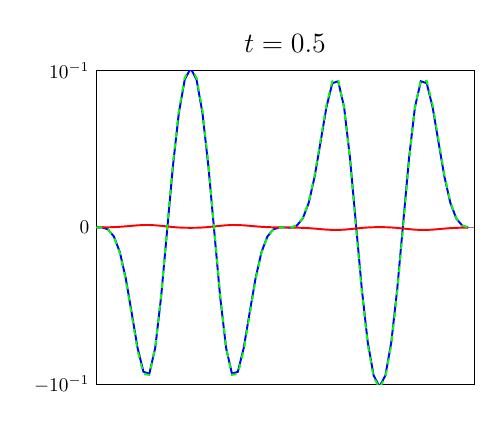
\begin{tikzpicture}[scale=0.7]

\begin{axis}[
    xtick = \empty,
    xmin = 0,
    xmax = 6.2832,
    ymin = -0.1,
    ymax = +0.1,
    ytick = {-0.1,0,0.1},
    yticklabels = {$-10^{-1}$,$0$,$10^{-1}$},
    scaled y ticks = false,
    scaled y ticks = false,
    title = {\Large $t = 0.5$},
  ]

\addplot[blue, line width=1pt] coordinates{
(0.0000e+00,6.0582e-12)
(9.8175e-02,6.4493e-05)
(1.9635e-01,-1.2452e-03)
(2.9452e-01,-5.7788e-03)
(3.9270e-01,-1.5693e-02)
(4.9087e-01,-3.2280e-02)
(5.8905e-01,-5.4213e-02)
(6.8722e-01,-7.6587e-02)
(7.8540e-01,-9.1961e-02)
(8.8357e-01,-9.3196e-02)
(9.8175e-01,-7.6651e-02)
(1.0799e+00,-4.4122e-02)
(1.1781e+00,-2.4484e-03)
(1.2763e+00,3.9226e-02)
(1.3744e+00,7.2989e-02)
(1.4726e+00,9.4253e-02)
(1.5708e+00,1.0142e-01)
(1.6690e+00,9.4253e-02)
(1.7671e+00,7.2989e-02)
(1.8653e+00,3.9226e-02)
(1.9635e+00,-2.4484e-03)
(2.0617e+00,-4.4122e-02)
(2.1598e+00,-7.6651e-02)
(2.2580e+00,-9.3196e-02)
(2.3562e+00,-9.1961e-02)
(2.4544e+00,-7.6587e-02)
(2.5525e+00,-5.4213e-02)
(2.6507e+00,-3.2280e-02)
(2.7489e+00,-1.5693e-02)
(2.8471e+00,-5.7788e-03)
(2.9452e+00,-1.2452e-03)
(3.0434e+00,6.4493e-05)
(3.1416e+00,6.6748e-12)
(3.2398e+00,-6.4493e-05)
(3.3379e+00,1.2452e-03)
(3.4361e+00,5.7788e-03)
(3.5343e+00,1.5693e-02)
(3.6325e+00,3.2280e-02)
(3.7306e+00,5.4213e-02)
(3.8288e+00,7.6587e-02)
(3.9270e+00,9.1961e-02)
(4.0252e+00,9.3196e-02)
(4.1233e+00,7.6651e-02)
(4.2215e+00,4.4122e-02)
(4.3197e+00,2.4484e-03)
(4.4179e+00,-3.9226e-02)
(4.5160e+00,-7.2989e-02)
(4.6142e+00,-9.4253e-02)
(4.7124e+00,-1.0142e-01)
(4.8106e+00,-9.4253e-02)
(4.9087e+00,-7.2989e-02)
(5.0069e+00,-3.9226e-02)
(5.1051e+00,2.4484e-03)
(5.2033e+00,4.4122e-02)
(5.3014e+00,7.6651e-02)
(5.3996e+00,9.3196e-02)
(5.4978e+00,9.1961e-02)
(5.5960e+00,7.6587e-02)
(5.6941e+00,5.4213e-02)
(5.7923e+00,3.2280e-02)
(5.8905e+00,1.5693e-02)
(5.9887e+00,5.7788e-03)
(6.0868e+00,1.2452e-03)
(6.1850e+00,-6.4493e-05)
};

\addplot[red, line width=1pt] coordinates{
(0.0000e+00,6.7339e-18)
(9.8175e-02,4.3333e-05)
(1.9635e-01,1.1058e-04)
(2.9452e-01,2.3031e-04)
(3.9270e-01,4.2984e-04)
(4.9087e-01,7.1540e-04)
(5.8905e-01,1.0514e-03)
(6.8722e-01,1.3614e-03)
(7.8540e-01,1.5567e-03)
(8.8357e-01,1.5722e-03)
(9.8175e-01,1.3903e-03)
(1.0799e+00,1.0511e-03)
(1.1781e+00,6.4307e-04)
(1.2763e+00,2.6721e-04)
(1.3744e+00,-7.6823e-06)
(1.4726e+00,-1.6322e-04)
(1.5708e+00,-2.1189e-04)
(1.6690e+00,-1.6322e-04)
(1.7671e+00,-7.6823e-06)
(1.8653e+00,2.6721e-04)
(1.9635e+00,6.4307e-04)
(2.0617e+00,1.0511e-03)
(2.1598e+00,1.3903e-03)
(2.2580e+00,1.5722e-03)
(2.3562e+00,1.5567e-03)
(2.4544e+00,1.3614e-03)
(2.5525e+00,1.0514e-03)
(2.6507e+00,7.1540e-04)
(2.7489e+00,4.2984e-04)
(2.8471e+00,2.3031e-04)
(2.9452e+00,1.1058e-04)
(3.0434e+00,4.3333e-05)
(3.1416e+00,-2.9592e-17)
(3.2398e+00,-4.3333e-05)
(3.3379e+00,-1.1058e-04)
(3.4361e+00,-2.3031e-04)
(3.5343e+00,-4.2984e-04)
(3.6325e+00,-7.1540e-04)
(3.7306e+00,-1.0514e-03)
(3.8288e+00,-1.3614e-03)
(3.9270e+00,-1.5567e-03)
(4.0252e+00,-1.5722e-03)
(4.1233e+00,-1.3903e-03)
(4.2215e+00,-1.0511e-03)
(4.3197e+00,-6.4307e-04)
(4.4179e+00,-2.6721e-04)
(4.5160e+00,7.6823e-06)
(4.6142e+00,1.6322e-04)
(4.7124e+00,2.1189e-04)
(4.8106e+00,1.6322e-04)
(4.9087e+00,7.6823e-06)
(5.0069e+00,-2.6721e-04)
(5.1051e+00,-6.4307e-04)
(5.2033e+00,-1.0511e-03)
(5.3014e+00,-1.3903e-03)
(5.3996e+00,-1.5722e-03)
(5.4978e+00,-1.5567e-03)
(5.5960e+00,-1.3614e-03)
(5.6941e+00,-1.0514e-03)
(5.7923e+00,-7.1540e-04)
(5.8905e+00,-4.2984e-04)
(5.9887e+00,-2.3031e-04)
(6.0868e+00,-1.1058e-04)
(6.1850e+00,-4.3333e-05)
};

\addplot[green, dashed, line width=1pt] coordinates{
(0.0000e+00,-3.9124e-12)
(9.8175e-02,2.0720e-05)
(1.9635e-01,-1.3715e-03)
(2.9452e-01,-6.0708e-03)
(3.9270e-01,-1.6268e-02)
(4.9087e-01,-3.3236e-02)
(5.8905e-01,-5.5539e-02)
(6.8722e-01,-7.8093e-02)
(7.8540e-01,-9.3289e-02)
(8.8357e-01,-9.3941e-02)
(9.8175e-01,-7.6532e-02)
(1.0799e+00,-4.3130e-02)
(1.1781e+00,-8.7651e-04)
(1.2763e+00,4.0917e-02)
(1.3744e+00,7.4420e-02)
(1.4726e+00,9.5324e-02)
(1.5708e+00,1.0233e-01)
(1.6690e+00,9.5324e-02)
(1.7671e+00,7.4420e-02)
(1.8653e+00,4.0917e-02)
(1.9635e+00,-8.7651e-04)
(2.0617e+00,-4.3130e-02)
(2.1598e+00,-7.6532e-02)
(2.2580e+00,-9.3941e-02)
(2.3562e+00,-9.3289e-02)
(2.4544e+00,-7.8093e-02)
(2.5525e+00,-5.5539e-02)
(2.6507e+00,-3.3236e-02)
(2.7489e+00,-1.6268e-02)
(2.8471e+00,-6.0708e-03)
(2.9452e+00,-1.3715e-03)
(3.0434e+00,2.0720e-05)
(3.1416e+00,5.6502e-13)
(3.2398e+00,-2.0720e-05)
(3.3379e+00,1.3715e-03)
(3.4361e+00,6.0708e-03)
(3.5343e+00,1.6268e-02)
(3.6325e+00,3.3236e-02)
(3.7306e+00,5.5539e-02)
(3.8288e+00,7.8093e-02)
(3.9270e+00,9.3289e-02)
(4.0252e+00,9.3941e-02)
(4.1233e+00,7.6532e-02)
(4.2215e+00,4.3130e-02)
(4.3197e+00,8.7651e-04)
(4.4179e+00,-4.0917e-02)
(4.5160e+00,-7.4420e-02)
(4.6142e+00,-9.5324e-02)
(4.7124e+00,-1.0233e-01)
(4.8106e+00,-9.5324e-02)
(4.9087e+00,-7.4420e-02)
(5.0069e+00,-4.0917e-02)
(5.1051e+00,8.7651e-04)
(5.2033e+00,4.3130e-02)
(5.3014e+00,7.6532e-02)
(5.3996e+00,9.3941e-02)
(5.4978e+00,9.3289e-02)
(5.5960e+00,7.8093e-02)
(5.6941e+00,5.5539e-02)
(5.7923e+00,3.3236e-02)
(5.8905e+00,1.6268e-02)
(5.9887e+00,6.0708e-03)
(6.0868e+00,1.3715e-03)
(6.1850e+00,-2.0720e-05)
};

\end{axis}



\end{tikzpicture}

  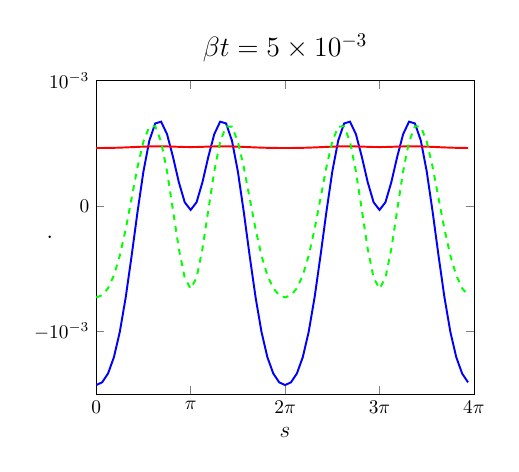
\begin{tikzpicture}[scale=0.7]

\begin{axis}[
    xmin = 0,
    xmax = 6.2832,
    xtick = {0,1.5708,3.1416,4.7124,6.2832},
    xticklabels = {$0$, $\pi$, $2\pi$, $3\pi$, $4\pi$},
    xlabel = {\large $s$},
    ymin = -0.0015,
    ymax = +0.001,
    ytick = {-0.001,0,0.001},
    yticklabels = {$-10^{-3}$,$0$,$10^{-3}$},
    ylabel = {\large $\uu \cdot \nn$},
    ylabel near ticks,
    ylabel shift = {-18pt},
    scaled y ticks = false,
    title = {\Large $\beta t = 5 \times 10^{-3}$},
  ]

\addplot[blue, line width=1pt] coordinates{
(0.0000e+00,-1.4252e-03)
(9.8175e-02,-1.4035e-03)
(1.9635e-01,-1.3334e-03)
(2.9452e-01,-1.2031e-03)
(3.9270e-01,-1.0011e-03)
(4.9087e-01,-7.2625e-04)
(5.8905e-01,-3.9562e-04)
(6.8722e-01,-4.5522e-05)
(7.8540e-01,2.7595e-04)
(8.8357e-01,5.2203e-04)
(9.8175e-01,6.5904e-04)
(1.0799e+00,6.7307e-04)
(1.1781e+00,5.7336e-04)
(1.2763e+00,3.9382e-04)
(1.3744e+00,1.9062e-04)
(1.4726e+00,3.0662e-05)
(1.5708e+00,-3.0007e-05)
(1.6690e+00,3.0662e-05)
(1.7671e+00,1.9062e-04)
(1.8653e+00,3.9382e-04)
(1.9635e+00,5.7336e-04)
(2.0617e+00,6.7307e-04)
(2.1598e+00,6.5904e-04)
(2.2580e+00,5.2203e-04)
(2.3562e+00,2.7595e-04)
(2.4544e+00,-4.5522e-05)
(2.5525e+00,-3.9562e-04)
(2.6507e+00,-7.2625e-04)
(2.7489e+00,-1.0011e-03)
(2.8471e+00,-1.2031e-03)
(2.9452e+00,-1.3334e-03)
(3.0434e+00,-1.4035e-03)
(3.1416e+00,-1.4252e-03)
(3.2398e+00,-1.4035e-03)
(3.3379e+00,-1.3334e-03)
(3.4361e+00,-1.2031e-03)
(3.5343e+00,-1.0011e-03)
(3.6325e+00,-7.2625e-04)
(3.7306e+00,-3.9562e-04)
(3.8288e+00,-4.5522e-05)
(3.9270e+00,2.7595e-04)
(4.0252e+00,5.2203e-04)
(4.1233e+00,6.5904e-04)
(4.2215e+00,6.7307e-04)
(4.3197e+00,5.7336e-04)
(4.4179e+00,3.9382e-04)
(4.5160e+00,1.9062e-04)
(4.6142e+00,3.0662e-05)
(4.7124e+00,-3.0007e-05)
(4.8106e+00,3.0662e-05)
(4.9087e+00,1.9062e-04)
(5.0069e+00,3.9382e-04)
(5.1051e+00,5.7336e-04)
(5.2033e+00,6.7307e-04)
(5.3014e+00,6.5904e-04)
(5.3996e+00,5.2203e-04)
(5.4978e+00,2.7595e-04)
(5.5960e+00,-4.5522e-05)
(5.6941e+00,-3.9562e-04)
(5.7923e+00,-7.2625e-04)
(5.8905e+00,-1.0011e-03)
(5.9887e+00,-1.2031e-03)
(6.0868e+00,-1.3334e-03)
(6.1850e+00,-1.4035e-03)
};

\addplot[red, line width=1pt] coordinates{
(0.0000e+00,4.6324e-04)
(9.8175e-02,4.6339e-04)
(1.9635e-01,4.6387e-04)
(2.9452e-01,4.6475e-04)
(3.9270e-01,4.6609e-04)
(4.9087e-01,4.6787e-04)
(5.8905e-01,4.6994e-04)
(6.8722e-01,4.7207e-04)
(7.8540e-01,4.7399e-04)
(8.8357e-01,4.7546e-04)
(9.8175e-01,4.7630e-04)
(1.0799e+00,4.7637e-04)
(1.1781e+00,4.7565e-04)
(1.2763e+00,4.7429e-04)
(1.3744e+00,4.7265e-04)
(1.4726e+00,4.7130e-04)
(1.5708e+00,4.7077e-04)
(1.6690e+00,4.7130e-04)
(1.7671e+00,4.7265e-04)
(1.8653e+00,4.7429e-04)
(1.9635e+00,4.7565e-04)
(2.0617e+00,4.7637e-04)
(2.1598e+00,4.7630e-04)
(2.2580e+00,4.7546e-04)
(2.3562e+00,4.7399e-04)
(2.4544e+00,4.7207e-04)
(2.5525e+00,4.6994e-04)
(2.6507e+00,4.6787e-04)
(2.7489e+00,4.6609e-04)
(2.8471e+00,4.6475e-04)
(2.9452e+00,4.6387e-04)
(3.0434e+00,4.6339e-04)
(3.1416e+00,4.6324e-04)
(3.2398e+00,4.6339e-04)
(3.3379e+00,4.6387e-04)
(3.4361e+00,4.6475e-04)
(3.5343e+00,4.6609e-04)
(3.6325e+00,4.6787e-04)
(3.7306e+00,4.6994e-04)
(3.8288e+00,4.7207e-04)
(3.9270e+00,4.7399e-04)
(4.0252e+00,4.7546e-04)
(4.1233e+00,4.7630e-04)
(4.2215e+00,4.7637e-04)
(4.3197e+00,4.7565e-04)
(4.4179e+00,4.7429e-04)
(4.5160e+00,4.7265e-04)
(4.6142e+00,4.7130e-04)
(4.7124e+00,4.7077e-04)
(4.8106e+00,4.7130e-04)
(4.9087e+00,4.7265e-04)
(5.0069e+00,4.7429e-04)
(5.1051e+00,4.7565e-04)
(5.2033e+00,4.7637e-04)
(5.3014e+00,4.7630e-04)
(5.3996e+00,4.7546e-04)
(5.4978e+00,4.7399e-04)
(5.5960e+00,4.7207e-04)
(5.6941e+00,4.6994e-04)
(5.7923e+00,4.6787e-04)
(5.8905e+00,4.6609e-04)
(5.9887e+00,4.6475e-04)
(6.0868e+00,4.6387e-04)
(6.1850e+00,4.6339e-04)
};

\addplot[green, dashed, line width=1pt] coordinates{
(0.0000e+00,-7.2674e-04)
(9.8175e-02,-7.0951e-04)
(1.9635e-01,-6.5403e-04)
(2.9452e-01,-5.5135e-04)
(3.9270e-01,-3.9376e-04)
(4.9087e-01,-1.8298e-04)
(5.8905e-01,6.3302e-05)
(6.8722e-01,3.1063e-04)
(7.8540e-01,5.1478e-04)
(8.8357e-01,6.3332e-04)
(9.8175e-01,6.3615e-04)
(1.0799e+00,5.1265e-04)
(1.1781e+00,2.7661e-04)
(1.2763e+00,-3.0169e-05)
(1.3744e+00,-3.3971e-04)
(1.4726e+00,-5.7126e-04)
(1.5708e+00,-6.5729e-04)
(1.6690e+00,-5.7126e-04)
(1.7671e+00,-3.3971e-04)
(1.8653e+00,-3.0169e-05)
(1.9635e+00,2.7661e-04)
(2.0617e+00,5.1265e-04)
(2.1598e+00,6.3615e-04)
(2.2580e+00,6.3332e-04)
(2.3562e+00,5.1478e-04)
(2.4544e+00,3.1063e-04)
(2.5525e+00,6.3302e-05)
(2.6507e+00,-1.8298e-04)
(2.7489e+00,-3.9376e-04)
(2.8471e+00,-5.5135e-04)
(2.9452e+00,-6.5403e-04)
(3.0434e+00,-7.0951e-04)
(3.1416e+00,-7.2674e-04)
(3.2398e+00,-7.0951e-04)
(3.3379e+00,-6.5403e-04)
(3.4361e+00,-5.5135e-04)
(3.5343e+00,-3.9376e-04)
(3.6325e+00,-1.8298e-04)
(3.7306e+00,6.3302e-05)
(3.8288e+00,3.1063e-04)
(3.9270e+00,5.1478e-04)
(4.0252e+00,6.3332e-04)
(4.1233e+00,6.3615e-04)
(4.2215e+00,5.1265e-04)
(4.3197e+00,2.7661e-04)
(4.4179e+00,-3.0169e-05)
(4.5160e+00,-3.3971e-04)
(4.6142e+00,-5.7126e-04)
(4.7124e+00,-6.5729e-04)
(4.8106e+00,-5.7126e-04)
(4.9087e+00,-3.3971e-04)
(5.0069e+00,-3.0169e-05)
(5.1051e+00,2.7661e-04)
(5.2033e+00,5.1265e-04)
(5.3014e+00,6.3615e-04)
(5.3996e+00,6.3332e-04)
(5.4978e+00,5.1478e-04)
(5.5960e+00,3.1063e-04)
(5.6941e+00,6.3302e-05)
(5.7923e+00,-1.8298e-04)
(5.8905e+00,-3.9376e-04)
(5.9887e+00,-5.5135e-04)
(6.0868e+00,-6.5403e-04)
(6.1850e+00,-7.0951e-04)
};

\end{axis}


\end{tikzpicture}

  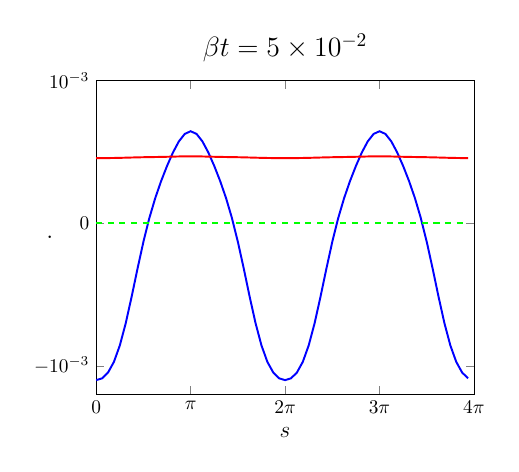
\begin{tikzpicture}[scale=0.7]


\begin{axis}[
    xmin = 0,
    xmax = 6.2832,
    xtick = {0,1.5708,3.1416,4.7124,6.2832},
    xticklabels = {$0$, $\pi$, $2\pi$, $3\pi$, $4\pi$},
    xlabel = {\large $s$},
    ymin = -0.0012,
    ymax = +0.001,
    ytick = {-0.001,0,0.001},
    yticklabels = {$-10^{-3}$,$0$,$10^{-3}$},
    ylabel = {\large $\uu \cdot \nn$},
    ylabel near ticks,
    ylabel shift = {-18pt},
    scaled y ticks = false,
    title = {\Large $\beta t = 5 \times 10^{-2}$},
  ]

\addplot[blue, line width=1pt] coordinates{
(0.0000e+00,-1.0996e-03)
(9.8175e-02,-1.0870e-03)
(1.9635e-01,-1.0466e-03)
(2.9452e-01,-9.7170e-04)
(3.9270e-01,-8.5638e-04)
(4.9087e-01,-7.0082e-04)
(5.8905e-01,-5.1507e-04)
(6.8722e-01,-3.1782e-04)
(7.8540e-01,-1.2954e-04)
(8.8357e-01,3.6091e-05)
(9.8175e-01,1.7622e-04)
(1.0799e+00,2.9597e-04)
(1.1781e+00,4.0183e-04)
(1.2763e+00,4.9586e-04)
(1.3744e+00,5.7370e-04)
(1.4726e+00,6.2639e-04)
(1.5708e+00,6.4517e-04)
(1.6690e+00,6.2639e-04)
(1.7671e+00,5.7370e-04)
(1.8653e+00,4.9586e-04)
(1.9635e+00,4.0183e-04)
(2.0617e+00,2.9597e-04)
(2.1598e+00,1.7622e-04)
(2.2580e+00,3.6091e-05)
(2.3562e+00,-1.2954e-04)
(2.4544e+00,-3.1782e-04)
(2.5525e+00,-5.1507e-04)
(2.6507e+00,-7.0082e-04)
(2.7489e+00,-8.5638e-04)
(2.8471e+00,-9.7170e-04)
(2.9452e+00,-1.0466e-03)
(3.0434e+00,-1.0870e-03)
(3.1416e+00,-1.0996e-03)
(3.2398e+00,-1.0870e-03)
(3.3379e+00,-1.0466e-03)
(3.4361e+00,-9.7170e-04)
(3.5343e+00,-8.5638e-04)
(3.6325e+00,-7.0082e-04)
(3.7306e+00,-5.1507e-04)
(3.8288e+00,-3.1782e-04)
(3.9270e+00,-1.2954e-04)
(4.0252e+00,3.6091e-05)
(4.1233e+00,1.7622e-04)
(4.2215e+00,2.9597e-04)
(4.3197e+00,4.0183e-04)
(4.4179e+00,4.9586e-04)
(4.5160e+00,5.7370e-04)
(4.6142e+00,6.2639e-04)
(4.7124e+00,6.4517e-04)
(4.8106e+00,6.2639e-04)
(4.9087e+00,5.7370e-04)
(5.0069e+00,4.9586e-04)
(5.1051e+00,4.0183e-04)
(5.2033e+00,2.9597e-04)
(5.3014e+00,1.7622e-04)
(5.3996e+00,3.6091e-05)
(5.4978e+00,-1.2954e-04)
(5.5960e+00,-3.1782e-04)
(5.6941e+00,-5.1507e-04)
(5.7923e+00,-7.0082e-04)
(5.8905e+00,-8.5638e-04)
(5.9887e+00,-9.7170e-04)
(6.0868e+00,-1.0466e-03)
(6.1850e+00,-1.0870e-03)
};

\addplot[red, line width=1pt] coordinates{
(0.0000e+00,4.5667e-04)
(9.8175e-02,4.5678e-04)
(1.9635e-01,4.5711e-04)
(2.9452e-01,4.5772e-04)
(3.9270e-01,4.5862e-04)
(4.9087e-01,4.5975e-04)
(5.8905e-01,4.6097e-04)
(6.8722e-01,4.6210e-04)
(7.8540e-01,4.6302e-04)
(8.8357e-01,4.6376e-04)
(9.8175e-01,4.6444e-04)
(1.0799e+00,4.6521e-04)
(1.1781e+00,4.6616e-04)
(1.2763e+00,4.6723e-04)
(1.3744e+00,4.6829e-04)
(1.4726e+00,4.6908e-04)
(1.5708e+00,4.6938e-04)
(1.6690e+00,4.6908e-04)
(1.7671e+00,4.6829e-04)
(1.8653e+00,4.6723e-04)
(1.9635e+00,4.6616e-04)
(2.0617e+00,4.6521e-04)
(2.1598e+00,4.6444e-04)
(2.2580e+00,4.6376e-04)
(2.3562e+00,4.6302e-04)
(2.4544e+00,4.6210e-04)
(2.5525e+00,4.6097e-04)
(2.6507e+00,4.5975e-04)
(2.7489e+00,4.5862e-04)
(2.8471e+00,4.5772e-04)
(2.9452e+00,4.5711e-04)
(3.0434e+00,4.5678e-04)
(3.1416e+00,4.5667e-04)
(3.2398e+00,4.5678e-04)
(3.3379e+00,4.5711e-04)
(3.4361e+00,4.5772e-04)
(3.5343e+00,4.5862e-04)
(3.6325e+00,4.5975e-04)
(3.7306e+00,4.6097e-04)
(3.8288e+00,4.6210e-04)
(3.9270e+00,4.6302e-04)
(4.0252e+00,4.6376e-04)
(4.1233e+00,4.6444e-04)
(4.2215e+00,4.6521e-04)
(4.3197e+00,4.6616e-04)
(4.4179e+00,4.6723e-04)
(4.5160e+00,4.6829e-04)
(4.6142e+00,4.6908e-04)
(4.7124e+00,4.6938e-04)
(4.8106e+00,4.6908e-04)
(4.9087e+00,4.6829e-04)
(5.0069e+00,4.6723e-04)
(5.1051e+00,4.6616e-04)
(5.2033e+00,4.6521e-04)
(5.3014e+00,4.6444e-04)
(5.3996e+00,4.6376e-04)
(5.4978e+00,4.6302e-04)
(5.5960e+00,4.6210e-04)
(5.6941e+00,4.6097e-04)
(5.7923e+00,4.5975e-04)
(5.8905e+00,4.5862e-04)
(5.9887e+00,4.5772e-04)
(6.0868e+00,4.5711e-04)
(6.1850e+00,4.5678e-04)
};

\addplot[green, dashed, line width=1pt] coordinates{
(0.0000e+00,-2.3701e-12)
(9.8175e-02,-5.1013e-12)
(1.9635e-01,-2.1890e-12)
(2.9452e-01,-3.5219e-12)
(3.9270e-01,-1.5410e-12)
(4.9087e-01,-1.8243e-12)
(5.8905e-01,-4.6256e-13)
(6.8722e-01,8.3140e-13)
(7.8540e-01,1.0570e-12)
(8.8357e-01,2.3248e-12)
(9.8175e-01,2.1470e-12)
(1.0799e+00,3.2332e-12)
(1.1781e+00,2.3841e-12)
(1.2763e+00,3.6752e-12)
(1.3744e+00,2.7500e-12)
(1.4726e+00,3.8911e-12)
(1.5708e+00,3.0465e-12)
(1.6690e+00,3.7839e-12)
(1.7671e+00,2.9670e-12)
(1.8653e+00,3.3832e-12)
(1.9635e+00,2.5833e-12)
(2.0617e+00,3.1272e-12)
(2.1598e+00,1.9943e-12)
(2.2580e+00,2.8072e-12)
(2.3562e+00,4.5835e-13)
(2.4544e+00,1.8049e-12)
(2.5525e+00,-1.7784e-12)
(2.6507e+00,4.5430e-13)
(2.7489e+00,-4.4271e-12)
(2.8471e+00,-1.2356e-12)
(2.9452e+00,-4.6053e-12)
(3.0434e+00,-2.1283e-12)
(3.1416e+00,-5.5059e-12)
(3.2398e+00,-3.2576e-12)
(3.3379e+00,-2.5917e-12)
(3.4361e+00,-3.6846e-12)
(3.5343e+00,-1.2203e-12)
(3.6325e+00,-2.5257e-12)
(3.7306e+00,4.3051e-13)
(3.8288e+00,-1.0295e-13)
(3.9270e+00,2.0464e-12)
(4.0252e+00,1.3831e-12)
(4.1233e+00,3.1439e-12)
(4.2215e+00,2.1068e-12)
(4.3197e+00,3.5191e-12)
(4.4179e+00,2.5897e-12)
(4.5160e+00,3.8035e-12)
(4.6142e+00,2.9385e-12)
(4.7124e+00,3.9496e-12)
(4.8106e+00,2.9646e-12)
(4.9087e+00,3.7350e-12)
(5.0069e+00,2.6137e-12)
(5.1051e+00,3.3981e-12)
(5.2033e+00,2.3594e-12)
(5.3014e+00,2.9610e-12)
(5.3996e+00,1.6281e-12)
(5.4978e+00,1.7719e-12)
(5.5960e+00,1.6160e-13)
(5.6941e+00,-2.2854e-13)
(5.7923e+00,-1.1349e-12)
(5.8905e+00,-2.8796e-12)
(5.9887e+00,-2.9905e-12)
(6.0868e+00,-2.1672e-12)
(6.1850e+00,-5.0508e-12)
};

\end{axis}

\end{tikzpicture}

  \fi
  \caption{\label{fig:vesVelocity} The velocity contributions due to
  semi-permeability (red) and force balance (blue). The green dashed
  line is the velocity of an impermeable vesicle with the same initial
  shape as the semi-permeable vesicle.}
\end{figure}

\begin{figure}[htp]
  \ifTikz
  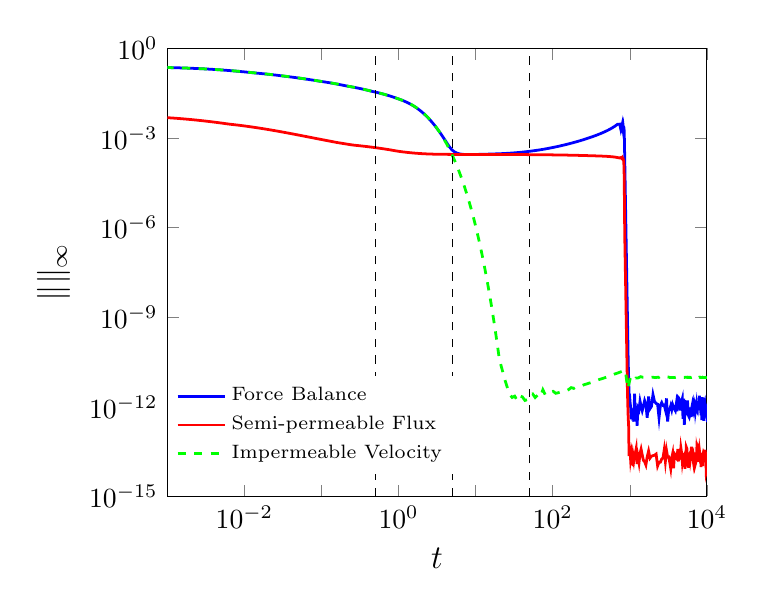
\begin{tikzpicture}[scale=1]

  \begin{axis}[
    name = maxPlot,
    xmin = 1e-3,
    xmax = 10000,
    ymin = 1e-15,
    ymax = 1e0,
    xmode = log,
    ymode = log,
    xminorticks = false,
    yminorticks = false,
    xtick = {1e-3,1e-2,1e-1,1e0,1e1,1e2,1e3,1e4},
    xticklabels = {,$10^{-2}$,,$10^0$,,$10^2$,,$10^4$},
    xlabel = {\large $t$},
    ylabel = {\large $\|\uu\|_\infty$},
    ylabel near ticks,
    legend entries = {Force Balance,
    Semi-permeable Flux,Impermeable Velocity},
    legend cell align=left,
    legend style={draw=none,font=\scriptsize},
    legend style={at={(0.0,0.05)},anchor=south west}
  ]

\addplot[blue, line width=1pt] coordinates{
(0.0000e+00,2.5143e-01)
(6.4149e-05,2.4906e-01)
(1.2188e-04,2.4693e-01)
(1.8424e-04,2.4478e-01)
(2.5158e-04,2.4254e-01)
(3.2431e-04,2.4022e-01)
(4.0286e-04,2.3783e-01)
(4.8769e-04,2.3537e-01)
(5.7930e-04,2.3284e-01)
(6.7825e-04,2.3024e-01)
(7.8511e-04,2.2773e-01)
(9.0052e-04,2.2619e-01)
(1.0252e-03,2.2455e-01)
(1.1598e-03,2.2283e-01)
(1.3052e-03,2.2100e-01)
(1.4622e-03,2.1908e-01)
(1.6318e-03,2.1706e-01)
(1.8149e-03,2.1494e-01)
(2.0127e-03,2.1273e-01)
(2.2263e-03,2.1043e-01)
(2.4570e-03,2.0804e-01)
(2.7062e-03,2.0557e-01)
(2.9753e-03,2.0301e-01)
(3.2659e-03,2.0037e-01)
(3.5798e-03,1.9766e-01)
(3.9188e-03,1.9487e-01)
(4.2849e-03,1.9201e-01)
(4.6803e-03,1.8909e-01)
(5.1073e-03,1.8610e-01)
(5.5685e-03,1.8306e-01)
(6.0666e-03,1.7997e-01)
(6.6045e-03,1.7683e-01)
(7.1855e-03,1.7365e-01)
(7.8129e-03,1.7043e-01)
(8.4905e-03,1.6718e-01)
(9.2224e-03,1.6390e-01)
(9.9991e-03,1.6066e-01)
(1.0827e-02,1.5743e-01)
(1.1702e-02,1.5426e-01)
(1.2641e-02,1.5108e-01)
(1.3621e-02,1.4800e-01)
(1.4679e-02,1.4543e-01)
(1.5779e-02,1.4296e-01)
(1.6968e-02,1.4043e-01)
(1.8208e-02,1.3794e-01)
(1.9547e-02,1.3539e-01)
(2.0933e-02,1.3290e-01)
(2.2430e-02,1.3035e-01)
(2.3996e-02,1.2782e-01)
(2.5687e-02,1.2523e-01)
(2.7422e-02,1.2273e-01)
(2.9295e-02,1.2015e-01)
(3.1276e-02,1.1758e-01)
(3.3376e-02,1.1510e-01)
(3.5593e-02,1.1281e-01)
(3.7949e-02,1.1053e-01)
(4.0425e-02,1.0827e-01)
(4.3074e-02,1.0599e-01)
(4.5826e-02,1.0377e-01)
(4.8797e-02,1.0149e-01)
(5.1865e-02,9.9283e-02)
(5.5178e-02,9.7024e-02)
(5.8630e-02,9.4806e-02)
(6.2358e-02,9.2538e-02)
(6.6187e-02,9.0543e-02)
(7.0322e-02,8.8527e-02)
(7.4666e-02,8.6516e-02)
(7.9318e-02,8.4459e-02)
(8.4141e-02,8.2434e-02)
(8.9350e-02,8.0349e-02)
(9.4748e-02,7.8401e-02)
(1.0058e-01,7.6656e-02)
(1.0663e-01,7.4942e-02)
(1.1316e-01,7.3178e-02)
(1.1994e-01,7.1447e-02)
(1.2725e-01,6.9669e-02)
(1.3486e-01,6.7918e-02)
(1.4308e-01,6.6121e-02)
(1.5159e-01,6.4360e-02)
(1.6079e-01,6.2557e-02)
(1.7039e-01,6.0778e-02)
(1.8076e-01,5.8961e-02)
(1.9148e-01,5.7215e-02)
(2.0304e-01,5.5535e-02)
(2.1521e-01,5.3906e-02)
(2.2829e-01,5.2503e-02)
(2.4187e-01,5.1119e-02)
(2.5654e-01,4.9696e-02)
(2.7191e-01,4.8285e-02)
(2.8850e-01,4.6839e-02)
(3.0579e-01,4.5415e-02)
(3.2446e-01,4.3960e-02)
(3.4425e-01,4.2507e-02)
(3.6555e-01,4.1032e-02)
(3.8802e-01,3.9571e-02)
(4.1229e-01,3.8090e-02)
(4.3823e-01,3.6663e-02)
(4.6618e-01,3.5256e-02)
(4.9600e-01,3.4003e-02)
(5.2821e-01,3.2752e-02)
(5.6259e-01,3.1488e-02)
(5.9972e-01,3.0196e-02)
(6.3901e-01,2.8902e-02)
(6.8145e-01,2.7582e-02)
(7.2600e-01,2.6334e-02)
(7.7412e-01,2.5064e-02)
(8.2397e-01,2.3816e-02)
(8.7782e-01,2.2537e-02)
(9.3363e-01,2.1296e-02)
(9.9391e-01,2.0088e-02)
(1.0560e+00,1.8988e-02)
(1.1231e+00,1.7874e-02)
(1.1935e+00,1.6761e-02)
(1.2696e+00,1.5602e-02)
(1.3493e+00,1.4457e-02)
(1.4353e+00,1.3282e-02)
(1.5282e+00,1.2101e-02)
(1.6286e+00,1.0921e-02)
(1.7370e+00,9.7569e-03)
(1.8540e+00,8.6206e-03)
(1.9805e+00,7.5269e-03)
(2.1170e+00,6.4886e-03)
(2.2645e+00,5.5180e-03)
(2.4237e+00,4.6252e-03)
(2.5957e+00,3.8178e-03)
(2.7815e+00,3.1018e-03)
(2.9821e+00,2.4840e-03)
(3.1988e+00,1.9590e-03)
(3.4328e+00,1.5197e-03)
(3.6855e+00,1.1615e-03)
(3.9584e+00,8.7926e-04)
(4.2532e+00,6.5945e-04)
(4.5716e+00,4.9988e-04)
(4.9154e+00,3.9480e-04)
(5.2868e+00,3.4142e-04)
(5.6878e+00,3.0992e-04)
(6.1209e+00,2.9209e-04)
(6.5887e+00,2.8332e-04)
(7.0939e+00,2.7818e-04)
(7.6395e+00,2.7687e-04)
(8.2288e+00,2.7653e-04)
(8.8652e+00,2.7680e-04)
(9.5525e+00,2.7748e-04)
(1.0295e+01,2.7843e-04)
(1.1096e+01,2.7956e-04)
(1.1962e+01,2.8085e-04)
(1.2897e+01,2.8227e-04)
(1.3907e+01,2.8381e-04)
(1.4998e+01,2.8549e-04)
(1.6176e+01,2.8731e-04)
(1.7448e+01,2.8927e-04)
(1.8822e+01,2.9140e-04)
(2.0306e+01,2.9371e-04)
(2.1908e+01,2.9620e-04)
(2.3639e+01,2.9906e-04)
(2.5509e+01,3.0232e-04)
(2.7527e+01,3.0615e-04)
(2.9708e+01,3.1030e-04)
(3.2062e+01,3.1485e-04)
(3.4605e+01,3.2004e-04)
(3.7352e+01,3.2577e-04)
(4.0318e+01,3.3238e-04)
(4.3522e+01,3.3966e-04)
(4.6982e+01,3.4754e-04)
(5.0718e+01,3.5606e-04)
(5.4754e+01,3.6529e-04)
(5.9112e+01,3.7527e-04)
(6.3819e+01,3.8609e-04)
(6.8903e+01,3.9780e-04)
(7.4393e+01,4.1106e-04)
(8.0323e+01,4.2566e-04)
(8.6727e+01,4.4148e-04)
(9.3643e+01,4.5860e-04)
(1.0111e+02,4.7716e-04)
(1.0918e+02,4.9728e-04)
(1.1789e+02,5.1910e-04)
(1.2730e+02,5.4279e-04)
(1.3746e+02,5.6851e-04)
(1.4844e+02,5.9648e-04)
(1.6029e+02,6.2690e-04)
(1.7309e+02,6.6004e-04)
(1.8692e+02,6.9619e-04)
(2.0185e+02,7.3567e-04)
(2.1798e+02,7.7888e-04)
(2.3539e+02,8.2627e-04)
(2.5420e+02,8.7860e-04)
(2.7452e+02,9.3646e-04)
(2.9646e+02,1.0004e-03)
(3.2015e+02,1.0713e-03)
(3.4574e+02,1.1504e-03)
(3.7338e+02,1.2392e-03)
(4.0323e+02,1.3396e-03)
(4.3546e+02,1.4544e-03)
(4.7028e+02,1.5874e-03)
(5.0788e+02,1.7443e-03)
(5.4849e+02,1.9321e-03)
(5.9234e+02,2.1625e-03)
(6.3971e+02,2.4532e-03)
(6.9087e+02,2.8309e-03)
(7.3860e+02,2.8717e-03)
(7.6471e+02,1.8870e-03)
(7.8821e+02,2.5831e-03)
(7.9978e+02,1.5132e-03)
(8.1019e+02,2.1951e-03)
(8.1786e+02,1.8397e-03)
(8.2476e+02,2.1848e-03)
(8.2894e+02,1.9639e-03)
(8.3270e+02,2.1935e-03)
(8.3676e+02,2.1955e-03)
(8.4008e+02,2.0963e-03)
(8.4307e+02,1.8359e-03)
(8.4630e+02,1.3692e-03)
(8.4979e+02,8.5321e-04)
(8.5355e+02,4.6151e-04)
(8.5762e+02,2.2880e-04)
(8.6201e+02,1.0623e-04)
(8.6676e+02,4.6574e-05)
(8.7188e+02,1.9205e-05)
(8.7741e+02,7.4416e-06)
(8.8339e+02,2.6891e-06)
(8.8984e+02,9.0581e-07)
(8.9681e+02,2.8105e-07)
(9.0434e+02,8.0677e-08)
(9.1247e+02,2.0930e-08)
(9.2125e+02,5.0195e-09)
(9.3074e+02,1.0411e-09)
(9.4098e+02,2.1553e-10)
(9.5204e+02,3.3127e-11)
(9.6399e+02,1.0173e-11)
(9.7689e+02,2.6156e-12)
(9.9082e+02,2.5647e-12)
(1.0059e+03,1.4604e-12)
(1.0221e+03,1.0297e-12)
(1.0397e+03,3.8532e-13)
(1.0586e+03,8.7966e-13)
(1.0791e+03,5.6448e-13)
(1.1012e+03,6.7332e-13)
(1.1251e+03,3.1864e-13)
(1.1509e+03,2.7655e-12)
(1.1787e+03,4.3047e-13)
(1.2088e+03,9.2874e-13)
(1.2413e+03,2.3389e-13)
(1.2764e+03,9.1925e-13)
(1.3143e+03,7.9248e-13)
(1.3552e+03,1.5394e-12)
(1.3994e+03,1.0368e-12)
(1.4472e+03,7.4452e-13)
(1.4987e+03,1.0463e-12)
(1.5544e+03,1.6068e-12)
(1.6145e+03,1.2030e-12)
(1.6795e+03,4.3113e-13)
(1.7496e+03,2.2264e-12)
(1.8254e+03,8.6291e-13)
(1.9072e+03,1.0332e-12)
(1.9955e+03,2.5592e-12)
(2.0910e+03,1.4926e-12)
(2.1910e+03,1.3019e-12)
(2.2910e+03,1.2244e-12)
(2.3910e+03,4.2932e-13)
(2.4910e+03,1.1290e-12)
(2.5910e+03,1.3855e-12)
(2.6910e+03,1.1209e-12)
(2.7910e+03,1.1519e-12)
(2.8910e+03,7.9919e-13)
(2.9910e+03,1.9182e-12)
(3.0910e+03,3.2355e-13)
(3.1910e+03,7.8306e-13)
(3.2910e+03,8.0543e-13)
(3.3910e+03,1.0720e-12)
(3.4910e+03,7.9869e-13)
(3.5910e+03,1.1848e-12)
(3.6910e+03,9.7610e-13)
(3.7910e+03,8.4733e-13)
(3.8910e+03,7.4753e-13)
(3.9910e+03,1.1734e-12)
(4.0910e+03,7.0933e-13)
(4.1910e+03,2.1420e-12)
(4.2910e+03,2.0005e-12)
(4.3910e+03,1.7126e-12)
(4.4910e+03,8.2398e-13)
(4.5910e+03,8.2245e-13)
(4.6910e+03,1.5379e-12)
(4.7910e+03,1.8778e-12)
(4.8910e+03,3.9299e-13)
(4.9910e+03,1.8851e-12)
(5.0910e+03,2.5074e-13)
(5.1910e+03,9.8207e-13)
(5.2910e+03,9.0016e-13)
(5.3910e+03,1.6474e-12)
(5.4910e+03,5.2017e-13)
(5.5910e+03,1.6420e-12)
(5.6910e+03,7.9097e-13)
(5.7910e+03,4.9046e-13)
(5.8910e+03,4.4748e-13)
(5.9910e+03,5.4278e-13)
(6.0910e+03,9.5033e-13)
(6.1910e+03,4.5112e-13)
(6.2910e+03,8.8500e-13)
(6.3910e+03,1.0037e-12)
(6.4910e+03,1.2334e-12)
(6.5910e+03,9.5577e-13)
(6.6910e+03,1.4078e-12)
(6.7910e+03,4.8365e-13)
(6.8910e+03,1.3804e-12)
(6.9910e+03,1.2211e-12)
(7.0910e+03,7.2179e-13)
(7.1910e+03,9.3724e-13)
(7.2910e+03,1.1978e-12)
(7.3910e+03,7.6460e-13)
(7.4910e+03,7.1138e-13)
(7.5910e+03,1.4478e-12)
(7.6910e+03,9.7540e-13)
(7.7910e+03,9.4444e-13)
(7.8910e+03,7.7455e-13)
(7.9910e+03,2.3758e-12)
(8.0910e+03,1.3559e-12)
(8.1910e+03,8.2851e-13)
(8.2910e+03,7.7395e-13)
(8.3910e+03,5.2508e-13)
(8.4910e+03,1.5877e-12)
(8.5910e+03,3.6241e-13)
(8.6910e+03,2.0898e-12)
(8.7910e+03,1.1283e-12)
(8.8910e+03,5.7107e-13)
(8.9910e+03,8.8000e-13)
(9.0910e+03,3.4033e-13)
(9.1910e+03,1.9988e-12)
(9.2910e+03,1.2492e-12)
(9.3910e+03,1.3974e-12)
(9.4910e+03,1.1016e-12)
(9.5910e+03,8.3162e-13)
(9.6910e+03,9.6957e-13)
(9.7910e+03,9.9004e-13)
(9.8910e+03,1.1992e-12)
(9.9910e+03,7.0748e-13)
(1.0091e+04,8.0575e-13)
(1.0191e+04,4.0864e-13)
(1.0291e+04,3.1129e-13)
(1.0391e+04,5.2996e-13)
(1.0491e+04,2.2481e-12)
(1.0591e+04,7.9016e-13)
(1.0691e+04,9.1354e-13)
(1.0791e+04,4.7389e-13)
(1.0891e+04,6.1893e-13)
(1.0991e+04,1.8346e-12)
(1.1091e+04,1.5432e-12)
(1.1191e+04,9.1388e-13)
(1.1291e+04,8.0937e-13)
(1.1391e+04,1.5291e-12)
(1.1491e+04,8.5536e-13)
(1.1591e+04,1.9577e-12)
(1.1691e+04,8.2352e-13)
(1.1791e+04,1.0942e-12)
(1.1891e+04,9.8388e-13)
(1.1991e+04,1.6554e-12)
(1.2091e+04,1.3927e-12)
(1.2191e+04,9.2175e-13)
(1.2291e+04,1.0800e-12)
(1.2391e+04,6.8912e-13)
(1.2491e+04,6.7045e-13)
(1.2591e+04,1.3170e-12)
(1.2691e+04,1.0000e-12)
(1.2791e+04,6.0368e-13)
(1.2891e+04,4.6551e-13)
(1.2991e+04,4.2708e-13)
(1.3091e+04,7.9265e-13)
(1.3191e+04,1.0978e-12)
(1.3291e+04,1.0257e-12)
(1.3391e+04,5.0769e-13)
(1.3491e+04,1.4083e-12)
(1.3591e+04,8.9094e-13)
(1.3691e+04,1.4698e-12)
(1.3791e+04,9.7415e-13)
(1.3891e+04,8.7689e-13)
(1.3991e+04,6.3129e-13)
(1.4091e+04,7.5509e-13)
(1.4191e+04,1.8049e-12)
(1.4291e+04,5.0680e-13)
(1.4391e+04,1.2294e-12)
(1.4491e+04,1.5597e-12)
(1.4591e+04,5.4681e-13)
(1.4691e+04,9.8953e-13)
(1.4791e+04,1.1934e-12)
(1.4891e+04,1.7594e-12)
(1.4991e+04,1.6216e-12)
(1.5091e+04,7.2236e-13)
(1.5191e+04,1.9573e-12)
(1.5291e+04,4.4939e-13)
(1.5391e+04,1.4691e-12)
(1.5491e+04,1.2943e-12)
(1.5591e+04,2.4329e-12)
(1.5691e+04,1.6416e-12)
(1.5791e+04,1.2694e-12)
(1.5891e+04,8.1613e-13)
(1.5991e+04,6.8194e-13)
(1.6091e+04,1.5994e-12)
(1.6191e+04,3.7993e-13)
(1.6291e+04,1.3779e-12)
(1.6391e+04,1.2776e-12)
(1.6491e+04,5.6385e-13)
(1.6591e+04,1.6089e-12)
(1.6691e+04,2.0244e-12)
(1.6791e+04,2.0989e-12)
(1.6891e+04,1.7240e-12)
(1.6991e+04,1.4830e-12)
(1.7091e+04,1.5747e-12)
(1.7191e+04,1.5543e-12)
(1.7291e+04,7.0006e-13)
(1.7391e+04,1.3472e-12)
(1.7491e+04,3.4862e-13)
(1.7591e+04,1.2367e-12)
(1.7691e+04,7.0192e-13)
(1.7791e+04,6.6082e-13)
(1.7891e+04,4.8511e-13)
(1.7991e+04,1.3491e-12)
(1.8091e+04,6.3469e-13)
(1.8191e+04,1.9423e-12)
(1.8291e+04,1.2199e-12)
(1.8391e+04,8.7569e-13)
(1.8491e+04,8.7707e-13)
(1.8591e+04,1.4653e-12)
(1.8691e+04,1.7261e-12)
(1.8791e+04,1.2364e-12)
(1.8891e+04,7.5528e-13)
(1.8991e+04,4.3179e-13)
(1.9091e+04,6.1800e-13)
(1.9191e+04,1.5140e-12)
(1.9291e+04,9.4249e-13)
(1.9391e+04,9.7265e-13)
(1.9491e+04,1.2219e-12)
(1.9591e+04,5.4964e-13)
(1.9691e+04,1.7148e-12)
(1.9791e+04,9.5472e-13)
(1.9891e+04,8.7837e-13)
(1.9991e+04,3.7547e-13)
(2.0000e+04,4.7031e-13)
};

\addplot[red, line width=1pt] coordinates{
(0.0000e+00,5.6693e-03)
(6.4149e-05,5.6070e-03)
(1.2188e-04,5.5480e-03)
(1.8424e-04,5.4839e-03)
(2.5158e-04,5.4139e-03)
(3.2431e-04,5.3388e-03)
(4.0286e-04,5.2588e-03)
(4.8769e-04,5.1745e-03)
(5.7930e-04,5.0862e-03)
(6.7825e-04,4.9945e-03)
(7.8511e-04,4.8999e-03)
(9.0052e-04,4.8029e-03)
(1.0252e-03,4.7041e-03)
(1.1598e-03,4.6038e-03)
(1.3052e-03,4.5025e-03)
(1.4622e-03,4.4006e-03)
(1.6318e-03,4.2983e-03)
(1.8149e-03,4.1958e-03)
(2.0127e-03,4.0934e-03)
(2.2263e-03,3.9913e-03)
(2.4570e-03,3.8896e-03)
(2.7062e-03,3.7884e-03)
(2.9753e-03,3.6879e-03)
(3.2659e-03,3.5882e-03)
(3.5798e-03,3.4893e-03)
(3.9188e-03,3.3914e-03)
(4.2849e-03,3.2947e-03)
(4.6803e-03,3.1991e-03)
(5.1073e-03,3.1048e-03)
(5.5685e-03,3.0120e-03)
(6.0666e-03,2.9206e-03)
(6.6045e-03,2.8397e-03)
(7.1855e-03,2.7728e-03)
(7.8129e-03,2.7048e-03)
(8.4905e-03,2.6360e-03)
(9.2224e-03,2.5666e-03)
(9.9991e-03,2.4980e-03)
(1.0827e-02,2.4299e-03)
(1.1702e-02,2.3632e-03)
(1.2641e-02,2.2969e-03)
(1.3621e-02,2.2328e-03)
(1.4679e-02,2.1688e-03)
(1.5779e-02,2.1072e-03)
(1.6968e-02,2.0459e-03)
(1.8208e-02,1.9868e-03)
(1.9547e-02,1.9280e-03)
(2.0933e-02,1.8720e-03)
(2.2430e-02,1.8163e-03)
(2.3996e-02,1.7626e-03)
(2.5687e-02,1.7094e-03)
(2.7422e-02,1.6591e-03)
(2.9295e-02,1.6092e-03)
(3.1276e-02,1.5608e-03)
(3.3376e-02,1.5136e-03)
(3.5593e-02,1.4679e-03)
(3.7949e-02,1.4234e-03)
(4.0425e-02,1.3804e-03)
(4.3074e-02,1.3383e-03)
(4.5826e-02,1.2981e-03)
(4.8797e-02,1.2584e-03)
(5.1865e-02,1.2207e-03)
(5.5178e-02,1.1835e-03)
(5.8630e-02,1.1479e-03)
(6.2358e-02,1.1129e-03)
(6.6187e-02,1.0797e-03)
(7.0322e-02,1.0471e-03)
(7.4666e-02,1.0156e-03)
(7.9318e-02,9.8477e-04)
(8.4141e-02,9.5547e-04)
(8.9350e-02,9.2771e-04)
(9.4748e-02,9.0119e-04)
(1.0058e-01,8.7493e-04)
(1.0663e-01,8.4973e-04)
(1.1316e-01,8.2472e-04)
(1.1994e-01,8.0175e-04)
(1.2725e-01,7.7887e-04)
(1.3486e-01,7.5669e-04)
(1.4308e-01,7.3449e-04)
(1.5159e-01,7.1299e-04)
(1.6079e-01,6.9400e-04)
(1.7039e-01,6.7759e-04)
(1.8076e-01,6.6117e-04)
(1.9148e-01,6.4538e-04)
(2.0304e-01,6.2948e-04)
(2.1521e-01,6.1393e-04)
(2.2829e-01,5.9921e-04)
(2.4187e-01,5.8578e-04)
(2.5654e-01,5.7434e-04)
(2.7191e-01,5.6389e-04)
(2.8850e-01,5.5493e-04)
(3.0579e-01,5.4624e-04)
(3.2446e-01,5.3727e-04)
(3.4425e-01,5.2835e-04)
(3.6555e-01,5.1914e-04)
(3.8802e-01,5.0994e-04)
(4.1229e-01,5.0036e-04)
(4.3823e-01,4.9059e-04)
(4.6618e-01,4.8044e-04)
(4.9600e-01,4.7006e-04)
(5.2821e-01,4.5973e-04)
(5.6259e-01,4.4973e-04)
(5.9972e-01,4.3934e-04)
(6.3901e-01,4.2889e-04)
(6.8145e-01,4.1805e-04)
(7.2600e-01,4.0731e-04)
(7.7412e-01,3.9623e-04)
(8.2397e-01,3.8552e-04)
(8.7782e-01,3.7451e-04)
(9.3363e-01,3.6409e-04)
(9.9391e-01,3.5501e-04)
(1.0560e+00,3.4721e-04)
(1.1231e+00,3.3996e-04)
(1.1935e+00,3.3369e-04)
(1.2696e+00,3.2756e-04)
(1.3493e+00,3.2206e-04)
(1.4353e+00,3.1687e-04)
(1.5282e+00,3.1206e-04)
(1.6286e+00,3.0756e-04)
(1.7370e+00,3.0343e-04)
(1.8540e+00,2.9968e-04)
(1.9805e+00,2.9630e-04)
(2.1170e+00,2.9331e-04)
(2.2645e+00,2.9068e-04)
(2.4237e+00,2.8840e-04)
(2.5957e+00,2.8645e-04)
(2.7815e+00,2.8481e-04)
(2.9821e+00,2.8345e-04)
(3.1988e+00,2.8233e-04)
(3.4328e+00,2.8143e-04)
(3.6855e+00,2.8072e-04)
(3.9584e+00,2.8016e-04)
(4.2532e+00,2.7973e-04)
(4.5716e+00,2.7940e-04)
(4.9154e+00,2.7916e-04)
(5.2868e+00,2.7897e-04)
(5.6878e+00,2.7883e-04)
(6.1209e+00,2.7872e-04)
(6.5887e+00,2.7863e-04)
(7.0939e+00,2.7855e-04)
(7.6395e+00,2.7847e-04)
(8.2288e+00,2.7840e-04)
(8.8652e+00,2.7833e-04)
(9.5525e+00,2.7825e-04)
(1.0295e+01,2.7817e-04)
(1.1096e+01,2.7808e-04)
(1.1962e+01,2.7799e-04)
(1.2897e+01,2.7788e-04)
(1.3907e+01,2.7777e-04)
(1.4998e+01,2.7765e-04)
(1.6176e+01,2.7753e-04)
(1.7448e+01,2.7739e-04)
(1.8822e+01,2.7724e-04)
(2.0306e+01,2.7708e-04)
(2.1908e+01,2.7690e-04)
(2.3639e+01,2.7671e-04)
(2.5509e+01,2.7651e-04)
(2.7527e+01,2.7629e-04)
(2.9708e+01,2.7605e-04)
(3.2062e+01,2.7580e-04)
(3.4605e+01,2.7552e-04)
(3.7352e+01,2.7523e-04)
(4.0318e+01,2.7490e-04)
(4.3522e+01,2.7456e-04)
(4.6982e+01,2.7419e-04)
(5.0718e+01,2.7378e-04)
(5.4754e+01,2.7335e-04)
(5.9112e+01,2.7288e-04)
(6.3819e+01,2.7238e-04)
(6.8903e+01,2.7183e-04)
(7.4393e+01,2.7124e-04)
(8.0323e+01,2.7065e-04)
(8.6727e+01,2.7007e-04)
(9.3643e+01,2.6944e-04)
(1.0111e+02,2.6876e-04)
(1.0918e+02,2.6803e-04)
(1.1789e+02,2.6724e-04)
(1.2730e+02,2.6639e-04)
(1.3746e+02,2.6548e-04)
(1.4844e+02,2.6449e-04)
(1.6029e+02,2.6342e-04)
(1.7309e+02,2.6227e-04)
(1.8692e+02,2.6103e-04)
(2.0185e+02,2.5986e-04)
(2.1798e+02,2.5863e-04)
(2.3539e+02,2.5730e-04)
(2.5420e+02,2.5586e-04)
(2.7452e+02,2.5437e-04)
(2.9646e+02,2.5292e-04)
(3.2015e+02,2.5134e-04)
(3.4574e+02,2.4980e-04)
(3.7338e+02,2.4820e-04)
(4.0323e+02,2.4643e-04)
(4.3546e+02,2.4443e-04)
(4.7028e+02,2.4214e-04)
(5.0788e+02,2.3947e-04)
(5.4849e+02,2.3624e-04)
(5.9234e+02,2.3218e-04)
(6.3971e+02,2.2674e-04)
(6.9087e+02,2.1876e-04)
(7.3860e+02,2.1165e-04)
(7.6471e+02,2.1850e-04)
(7.8821e+02,2.0199e-04)
(7.9978e+02,2.1512e-04)
(8.1019e+02,1.9615e-04)
(8.1786e+02,1.9725e-04)
(8.2476e+02,1.7795e-04)
(8.2894e+02,1.7558e-04)
(8.3270e+02,1.5295e-04)
(8.3676e+02,1.2683e-04)
(8.4008e+02,9.5715e-05)
(8.4307e+02,6.1539e-05)
(8.4630e+02,2.9768e-05)
(8.4979e+02,1.0317e-05)
(8.5355e+02,2.7336e-06)
(8.5762e+02,6.9224e-07)
(8.6201e+02,3.0044e-07)
(8.6676e+02,1.3603e-07)
(8.7188e+02,5.7548e-08)
(8.7741e+02,2.2651e-08)
(8.8339e+02,8.2446e-09)
(8.8984e+02,2.8171e-09)
(8.9681e+02,8.7232e-10)
(9.0434e+02,2.5644e-10)
(9.1247e+02,6.5383e-11)
(9.2125e+02,1.6783e-11)
(9.3074e+02,3.2506e-12)
(9.4098e+02,1.1296e-12)
(9.5204e+02,4.3169e-13)
(9.6399e+02,2.3733e-13)
(9.7689e+02,2.2621e-14)
(9.9082e+02,4.3649e-14)
(1.0059e+03,3.4117e-14)
(1.0221e+03,1.7449e-14)
(1.0397e+03,2.3844e-14)
(1.0586e+03,1.2719e-14)
(1.0791e+03,1.2123e-14)
(1.1012e+03,2.3179e-14)
(1.1251e+03,1.6207e-14)
(1.1509e+03,2.5628e-14)
(1.1787e+03,2.8429e-14)
(1.2088e+03,3.9962e-14)
(1.2413e+03,1.2196e-14)
(1.2764e+03,2.0626e-14)
(1.3143e+03,1.3292e-14)
(1.3552e+03,2.7086e-14)
(1.3994e+03,3.8263e-14)
(1.4472e+03,2.4673e-14)
(1.4987e+03,1.6260e-14)
(1.5544e+03,1.4749e-14)
(1.6145e+03,1.1371e-14)
(1.6795e+03,2.1419e-14)
(1.7496e+03,3.2947e-14)
(1.8254e+03,1.9222e-14)
(1.9072e+03,2.2400e-14)
(1.9955e+03,2.3172e-14)
(2.0910e+03,2.3993e-14)
(2.1910e+03,2.6299e-14)
(2.2910e+03,1.0545e-14)
(2.3910e+03,1.4095e-14)
(2.4910e+03,1.4118e-14)
(2.5910e+03,1.7952e-14)
(2.6910e+03,1.9555e-14)
(2.7910e+03,3.6036e-14)
(2.8910e+03,1.4932e-14)
(2.9910e+03,3.4162e-14)
(3.0910e+03,2.0982e-14)
(3.1910e+03,2.1237e-14)
(3.2910e+03,1.4081e-14)
(3.3910e+03,8.7783e-15)
(3.4910e+03,1.9536e-14)
(3.5910e+03,2.7275e-14)
(3.6910e+03,8.7754e-15)
(3.7910e+03,2.6815e-14)
(3.8910e+03,2.4278e-14)
(3.9910e+03,1.8711e-14)
(4.0910e+03,1.7574e-14)
(4.1910e+03,3.8939e-14)
(4.2910e+03,2.1952e-14)
(4.3910e+03,1.8438e-14)
(4.4910e+03,2.0446e-14)
(4.5910e+03,4.2310e-14)
(4.6910e+03,2.9090e-14)
(4.7910e+03,1.4671e-14)
(4.8910e+03,2.1928e-14)
(4.9910e+03,2.3796e-14)
(5.0910e+03,1.5050e-14)
(5.1910e+03,8.4461e-15)
(5.2910e+03,1.4975e-14)
(5.3910e+03,4.5208e-14)
(5.4910e+03,3.9769e-14)
(5.5910e+03,1.0303e-14)
(5.6910e+03,1.5348e-14)
(5.7910e+03,9.1048e-15)
(5.8910e+03,2.4236e-14)
(5.9910e+03,2.6767e-14)
(6.0910e+03,1.7249e-14)
(6.1910e+03,2.3393e-14)
(6.2910e+03,4.6190e-14)
(6.3910e+03,2.4691e-14)
(6.4910e+03,2.4260e-14)
(6.5910e+03,2.7087e-14)
(6.6910e+03,1.3509e-14)
(6.7910e+03,1.0599e-14)
(6.8910e+03,1.3049e-14)
(6.9910e+03,2.9886e-14)
(7.0910e+03,1.2369e-14)
(7.1910e+03,1.4245e-14)
(7.2910e+03,1.6823e-14)
(7.3910e+03,3.9814e-14)
(7.4910e+03,3.2972e-14)
(7.5910e+03,2.5795e-14)
(7.6910e+03,1.4391e-14)
(7.7910e+03,2.9495e-14)
(7.8910e+03,2.5102e-14)
(7.9910e+03,3.4773e-14)
(8.0910e+03,2.6366e-14)
(8.1910e+03,2.5085e-14)
(8.2910e+03,2.4418e-14)
(8.3910e+03,9.6396e-15)
(8.4910e+03,2.8596e-14)
(8.5910e+03,2.3453e-14)
(8.6910e+03,2.3874e-14)
(8.7910e+03,1.0467e-14)
(8.8910e+03,2.5197e-14)
(8.9910e+03,2.9020e-14)
(9.0910e+03,2.6943e-14)
(9.1910e+03,2.1377e-14)
(9.2910e+03,1.3795e-14)
(9.3910e+03,3.0234e-14)
(9.4910e+03,3.6269e-14)
(9.5910e+03,1.7869e-14)
(9.6910e+03,1.7195e-14)
(9.7910e+03,6.6374e-15)
(9.8910e+03,7.4312e-15)
(9.9910e+03,3.1134e-14)
(1.0091e+04,1.2721e-14)
(1.0191e+04,2.3357e-14)
(1.0291e+04,2.4906e-14)
(1.0391e+04,1.9568e-14)
(1.0491e+04,2.3754e-14)
(1.0591e+04,3.1157e-14)
(1.0691e+04,2.5085e-14)
(1.0791e+04,2.9293e-14)
(1.0891e+04,2.2021e-14)
(1.0991e+04,2.2934e-14)
(1.1091e+04,1.5633e-14)
(1.1191e+04,2.1718e-14)
(1.1291e+04,4.8615e-14)
(1.1391e+04,2.5722e-14)
(1.1491e+04,1.2631e-14)
(1.1591e+04,3.6677e-14)
(1.1691e+04,1.7100e-14)
(1.1791e+04,3.8447e-14)
(1.1891e+04,4.4168e-14)
(1.1991e+04,3.8039e-14)
(1.2091e+04,1.3166e-14)
(1.2191e+04,1.0820e-14)
(1.2291e+04,1.5829e-14)
(1.2391e+04,1.7789e-14)
(1.2491e+04,7.2545e-15)
(1.2591e+04,1.8568e-14)
(1.2691e+04,3.0936e-14)
(1.2791e+04,2.0484e-14)
(1.2891e+04,1.6596e-14)
(1.2991e+04,2.9214e-14)
(1.3091e+04,2.0248e-14)
(1.3191e+04,3.6711e-14)
(1.3291e+04,2.9857e-14)
(1.3391e+04,9.6160e-15)
(1.3491e+04,2.0237e-14)
(1.3591e+04,2.2302e-14)
(1.3691e+04,2.3002e-14)
(1.3791e+04,2.7511e-14)
(1.3891e+04,1.6357e-14)
(1.3991e+04,1.9212e-14)
(1.4091e+04,2.5781e-14)
(1.4191e+04,3.2396e-14)
(1.4291e+04,1.5631e-14)
(1.4391e+04,1.2267e-14)
(1.4491e+04,1.9854e-14)
(1.4591e+04,1.7628e-14)
(1.4691e+04,3.4073e-14)
(1.4791e+04,4.2443e-14)
(1.4891e+04,3.0432e-14)
(1.4991e+04,4.2351e-14)
(1.5091e+04,4.1907e-14)
(1.5191e+04,2.3215e-14)
(1.5291e+04,2.3100e-14)
(1.5391e+04,1.8164e-14)
(1.5491e+04,2.9011e-14)
(1.5591e+04,2.1870e-14)
(1.5691e+04,2.2520e-14)
(1.5791e+04,1.4747e-14)
(1.5891e+04,2.4073e-14)
(1.5991e+04,3.7654e-14)
(1.6091e+04,2.4416e-14)
(1.6191e+04,1.1497e-14)
(1.6291e+04,1.7328e-14)
(1.6391e+04,4.3015e-14)
(1.6491e+04,1.8581e-14)
(1.6591e+04,1.5256e-14)
(1.6691e+04,2.5442e-14)
(1.6791e+04,1.7565e-14)
(1.6891e+04,1.6557e-14)
(1.6991e+04,2.0475e-14)
(1.7091e+04,1.5720e-14)
(1.7191e+04,8.4512e-15)
(1.7291e+04,1.4006e-14)
(1.7391e+04,1.8519e-14)
(1.7491e+04,7.7379e-15)
(1.7591e+04,2.8026e-14)
(1.7691e+04,2.6360e-14)
(1.7791e+04,1.4545e-14)
(1.7891e+04,2.5924e-14)
(1.7991e+04,1.9612e-14)
(1.8091e+04,1.2754e-14)
(1.8191e+04,8.6501e-15)
(1.8291e+04,2.3384e-14)
(1.8391e+04,2.9081e-14)
(1.8491e+04,2.0677e-14)
(1.8591e+04,1.1112e-14)
(1.8691e+04,2.8848e-14)
(1.8791e+04,1.9517e-14)
(1.8891e+04,1.4772e-14)
(1.8991e+04,2.1345e-14)
(1.9091e+04,2.9260e-14)
(1.9191e+04,1.3769e-14)
(1.9291e+04,1.1431e-14)
(1.9391e+04,3.7128e-14)
(1.9491e+04,2.4117e-14)
(1.9591e+04,1.2209e-14)
(1.9691e+04,3.2980e-14)
(1.9791e+04,1.7004e-14)
(1.9891e+04,7.7523e-15)
(1.9991e+04,2.1033e-14)
(2.0000e+04,3.4849e-14)
};

\addplot[green, dashed, line width=1pt] coordinates{
(0.0000e+00,2.5098e-01)
(7.9049e-05,2.4823e-01)
(1.5019e-04,2.4578e-01)
(2.2703e-04,2.4332e-01)
(3.1001e-04,2.4076e-01)
(3.9963e-04,2.3814e-01)
(4.9642e-04,2.3544e-01)
(6.0096e-04,2.3267e-01)
(7.1386e-04,2.2984e-01)
(8.3578e-04,2.2695e-01)
(9.6747e-04,2.2505e-01)
(1.1097e-03,2.2328e-01)
(1.2633e-03,2.2141e-01)
(1.4292e-03,2.1945e-01)
(1.6083e-03,2.1738e-01)
(1.8018e-03,2.1521e-01)
(2.0108e-03,2.1294e-01)
(2.2364e-03,2.1058e-01)
(2.4802e-03,2.0813e-01)
(2.7434e-03,2.0559e-01)
(3.0277e-03,2.0297e-01)
(3.3348e-03,2.0026e-01)
(3.6664e-03,1.9748e-01)
(4.0245e-03,1.9462e-01)
(4.4113e-03,1.9170e-01)
(4.8290e-03,1.8871e-01)
(5.2801e-03,1.8566e-01)
(5.7674e-03,1.8256e-01)
(6.2936e-03,1.7940e-01)
(6.8619e-03,1.7620e-01)
(7.4756e-03,1.7296e-01)
(8.1385e-03,1.6969e-01)
(8.8544e-03,1.6639e-01)
(9.6276e-03,1.6306e-01)
(1.0429e-02,1.5984e-01)
(1.1295e-02,1.5660e-01)
(1.2214e-02,1.5340e-01)
(1.3192e-02,1.5022e-01)
(1.4225e-02,1.4709e-01)
(1.5331e-02,1.4437e-01)
(1.6488e-02,1.4187e-01)
(1.7738e-02,1.3932e-01)
(1.9029e-02,1.3683e-01)
(2.0424e-02,1.3428e-01)
(2.1890e-02,1.3174e-01)
(2.3464e-02,1.2917e-01)
(2.5097e-02,1.2664e-01)
(2.6859e-02,1.2406e-01)
(2.8694e-02,1.2151e-01)
(3.0676e-02,1.1890e-01)
(3.2723e-02,1.1635e-01)
(3.4934e-02,1.1395e-01)
(3.7243e-02,1.1167e-01)
(3.9737e-02,1.0936e-01)
(4.2293e-02,1.0713e-01)
(4.5055e-02,1.0486e-01)
(4.7967e-02,1.0260e-01)
(5.1066e-02,1.0034e-01)
(5.4316e-02,9.8096e-02)
(5.7805e-02,9.5823e-02)
(6.1408e-02,9.3609e-02)
(6.5298e-02,9.1347e-02)
(6.9355e-02,8.9278e-02)
(7.3737e-02,8.7235e-02)
(7.8235e-02,8.5243e-02)
(8.3094e-02,8.3187e-02)
(8.8208e-02,8.1133e-02)
(9.3669e-02,7.9046e-02)
(9.9365e-02,7.7232e-02)
(1.0552e-01,7.5475e-02)
(1.1184e-01,7.3764e-02)
(1.1868e-01,7.2004e-02)
(1.2587e-01,7.0250e-02)
(1.3357e-01,6.8467e-02)
(1.4158e-01,6.6710e-02)
(1.5024e-01,6.4908e-02)
(1.5921e-01,6.3143e-02)
(1.6889e-01,6.1337e-02)
(1.7902e-01,5.9555e-02)
(1.8995e-01,5.7736e-02)
(2.0124e-01,5.5975e-02)
(2.1344e-01,5.4293e-02)
(2.2629e-01,5.2798e-02)
(2.4007e-01,5.1392e-02)
(2.5445e-01,5.0000e-02)
(2.6998e-01,4.8570e-02)
(2.8618e-01,4.7158e-02)
(3.0368e-01,4.5712e-02)
(3.2208e-01,4.4277e-02)
(3.4196e-01,4.2812e-02)
(3.6284e-01,4.1364e-02)
(3.8539e-01,3.9891e-02)
(4.0944e-01,3.8418e-02)
(4.3536e-01,3.6930e-02)
(4.6292e-01,3.5511e-02)
(4.9269e-01,3.4157e-02)
(5.2462e-01,3.2921e-02)
(5.5898e-01,3.1659e-02)
(5.9572e-01,3.0383e-02)
(6.3524e-01,2.9084e-02)
(6.7718e-01,2.7782e-02)
(7.2235e-01,2.6465e-02)
(7.6958e-01,2.5224e-02)
(8.2059e-01,2.3952e-02)
(8.7343e-01,2.2703e-02)
(9.3049e-01,2.1424e-02)
(9.8957e-01,2.0216e-02)
(1.0534e+00,1.9058e-02)
(1.1195e+00,1.7981e-02)
(1.1909e+00,1.6853e-02)
(1.2660e+00,1.5728e-02)
(1.3470e+00,1.4563e-02)
(1.4332e+00,1.3401e-02)
(1.5262e+00,1.2221e-02)
(1.6266e+00,1.1043e-02)
(1.7351e+00,9.8758e-03)
(1.8523e+00,8.7355e-03)
(1.9788e+00,7.6349e-03)
(2.1155e+00,6.5880e-03)
(2.2631e+00,5.6074e-03)
(2.4225e+00,4.7028e-03)
(2.5946e+00,3.8825e-03)
(2.7805e+00,3.1517e-03)
(2.9813e+00,2.5129e-03)
(3.1982e+00,1.9657e-03)
(3.4324e+00,1.5067e-03)
(3.6854e+00,1.1301e-03)
(3.9585e+00,8.2839e-04)
(4.2536e+00,5.9253e-04)
(4.5722e+00,4.1293e-04)
(4.9163e+00,2.7991e-04)
(5.2880e+00,1.8423e-04)
(5.6894e+00,1.1754e-04)
(6.1229e+00,7.2550e-05)
(6.5911e+00,4.3221e-05)
(7.0967e+00,2.4795e-05)
(7.6428e+00,1.3666e-05)
(8.2326e+00,7.2190e-06)
(8.8696e+00,3.6443e-06)
(9.5575e+00,1.7531e-06)
(1.0300e+01,8.0117e-07)
(1.1103e+01,3.4671e-07)
(1.1969e+01,1.4160e-07)
(1.2905e+01,5.4375e-08)
(1.3916e+01,1.9557e-08)
(1.5008e+01,6.5601e-09)
(1.6187e+01,2.0439e-09)
(1.7460e+01,5.8862e-10)
(1.8835e+01,1.5597e-10)
(2.0320e+01,3.8143e-11)
(2.1924e+01,1.8633e-11)
(2.3657e+01,8.7763e-12)
(2.5528e+01,4.7407e-12)
(2.7548e+01,2.6355e-12)
(2.9730e+01,2.0559e-12)
(3.2087e+01,2.2771e-12)
(3.4632e+01,1.6226e-12)
(3.7381e+01,2.3248e-12)
(4.0350e+01,2.1554e-12)
(4.3557e+01,1.6344e-12)
(4.7020e+01,1.7455e-12)
(5.0759e+01,2.5639e-12)
(5.4799e+01,2.7186e-12)
(5.9161e+01,2.0402e-12)
(6.3872e+01,2.4824e-12)
(6.8960e+01,2.1381e-12)
(7.4455e+01,3.7182e-12)
(8.0390e+01,2.4513e-12)
(8.6800e+01,2.8169e-12)
(9.3722e+01,3.0758e-12)
(1.0120e+02,3.3028e-12)
(1.0927e+02,2.8365e-12)
(1.1799e+02,2.9590e-12)
(1.2741e+02,3.1587e-12)
(1.3758e+02,3.2125e-12)
(1.4857e+02,3.4191e-12)
(1.6043e+02,3.7651e-12)
(1.7324e+02,4.3911e-12)
(1.8708e+02,4.1412e-12)
(2.0203e+02,4.6815e-12)
(2.1817e+02,4.8861e-12)
(2.3560e+02,5.0417e-12)
(2.5442e+02,5.4703e-12)
(2.7476e+02,5.8246e-12)
(2.9671e+02,6.1999e-12)
(3.2043e+02,6.5984e-12)
(3.4604e+02,7.1861e-12)
(3.7370e+02,7.6200e-12)
(4.0358e+02,8.2710e-12)
(4.3584e+02,8.7611e-12)
(4.7069e+02,9.3601e-12)
(5.0832e+02,1.0088e-11)
(5.4897e+02,1.1181e-11)
(5.9286e+02,1.1686e-11)
(6.4027e+02,1.2610e-11)
(6.9147e+02,1.3457e-11)
(7.4677e+02,1.4485e-11)
(8.0649e+02,1.5671e-11)
(8.7098e+02,1.6867e-11)
(9.4064e+02,4.0698e-12)
(1.0159e+03,9.3937e-12)
(1.0971e+03,7.3120e-12)
(1.1849e+03,9.1161e-12)
(1.2796e+03,9.2852e-12)
(1.3796e+03,1.0204e-11)
(1.4796e+03,9.7565e-12)
(1.5796e+03,9.7371e-12)
(1.6796e+03,9.6417e-12)
(1.7796e+03,9.9750e-12)
(1.8796e+03,9.6146e-12)
(1.9796e+03,9.8207e-12)
(2.0796e+03,9.5693e-12)
(2.1796e+03,9.5532e-12)
(2.2796e+03,9.7414e-12)
(2.3796e+03,9.6510e-12)
(2.4796e+03,1.0366e-11)
(2.5796e+03,9.7363e-12)
(2.6796e+03,9.7004e-12)
(2.7796e+03,9.5434e-12)
(2.8796e+03,9.5641e-12)
(2.9796e+03,9.6679e-12)
(3.0796e+03,9.9416e-12)
(3.1796e+03,9.8994e-12)
(3.2796e+03,9.6315e-12)
(3.3796e+03,9.5663e-12)
(3.4796e+03,9.5860e-12)
(3.5796e+03,9.6156e-12)
(3.6796e+03,9.5202e-12)
(3.7796e+03,9.6394e-12)
(3.8796e+03,9.6259e-12)
(3.9796e+03,9.8050e-12)
(4.0796e+03,9.7616e-12)
(4.1796e+03,9.5942e-12)
(4.2796e+03,9.8353e-12)
(4.3796e+03,9.7715e-12)
(4.4796e+03,9.5369e-12)
(4.5796e+03,9.5675e-12)
(4.6796e+03,9.5829e-12)
(4.7796e+03,9.7260e-12)
(4.8796e+03,9.6628e-12)
(4.9796e+03,9.5908e-12)
(5.0796e+03,9.5705e-12)
(5.1796e+03,9.7122e-12)
(5.2796e+03,9.8086e-12)
(5.3796e+03,9.7163e-12)
(5.4796e+03,9.6569e-12)
(5.5796e+03,9.7917e-12)
(5.6796e+03,9.5615e-12)
(5.7796e+03,9.6810e-12)
(5.8796e+03,9.5562e-12)
(5.9796e+03,9.7869e-12)
(6.0796e+03,9.6950e-12)
(6.1796e+03,9.5704e-12)
(6.2796e+03,9.5730e-12)
(6.3796e+03,9.7137e-12)
(6.4796e+03,9.5541e-12)
(6.5796e+03,9.5534e-12)
(6.6796e+03,9.5564e-12)
(6.7796e+03,9.5413e-12)
(6.8796e+03,9.5431e-12)
(6.9796e+03,9.8308e-12)
(7.0796e+03,9.8837e-12)
(7.1796e+03,1.0448e-11)
(7.2796e+03,9.7986e-12)
(7.3796e+03,9.6981e-12)
(7.4796e+03,9.5304e-12)
(7.5796e+03,9.5552e-12)
(7.6796e+03,9.6131e-12)
(7.7796e+03,9.5730e-12)
(7.8796e+03,9.7423e-12)
(7.9796e+03,9.7285e-12)
(8.0796e+03,9.8376e-12)
(8.1796e+03,9.5912e-12)
(8.2796e+03,9.5550e-12)
(8.3796e+03,9.5594e-12)
(8.4796e+03,9.5739e-12)
(8.5796e+03,9.6410e-12)
(8.6796e+03,9.6251e-12)
(8.7796e+03,9.7819e-12)
(8.8796e+03,9.6298e-12)
(8.9796e+03,9.5849e-12)
(9.0796e+03,9.5444e-12)
(9.1796e+03,9.5641e-12)
(9.2796e+03,9.5916e-12)
(9.3796e+03,9.6237e-12)
(9.4796e+03,9.5538e-12)
(9.5796e+03,9.6400e-12)
(9.6796e+03,9.5797e-12)
(9.7796e+03,9.5703e-12)
(9.8796e+03,9.6225e-12)
(9.9796e+03,9.6496e-12)
(1.0080e+04,9.8844e-12)
(1.0180e+04,9.5379e-12)
(1.0280e+04,9.5550e-12)
(1.0380e+04,9.5713e-12)
(1.0480e+04,9.6333e-12)
(1.0580e+04,9.5724e-12)
(1.0680e+04,9.5701e-12)
(1.0780e+04,9.5285e-12)
(1.0880e+04,9.8690e-12)
(1.0980e+04,9.8649e-12)
(1.1080e+04,1.0032e-11)
(1.1180e+04,1.0056e-11)
(1.1280e+04,9.5417e-12)
(1.1380e+04,9.7058e-12)
(1.1480e+04,9.5483e-12)
(1.1580e+04,9.6052e-12)
(1.1680e+04,9.5557e-12)
(1.1780e+04,9.6531e-12)
(1.1880e+04,9.5540e-12)
(1.1980e+04,9.6653e-12)
(1.2080e+04,9.5918e-12)
(1.2180e+04,9.6198e-12)
(1.2280e+04,9.5496e-12)
(1.2380e+04,9.7144e-12)
(1.2480e+04,9.5753e-12)
(1.2580e+04,9.6531e-12)
(1.2680e+04,9.5840e-12)
(1.2780e+04,9.5498e-12)
(1.2880e+04,9.6000e-12)
(1.2980e+04,9.5583e-12)
(1.3080e+04,9.5210e-12)
(1.3180e+04,9.5396e-12)
(1.3280e+04,9.5434e-12)
(1.3380e+04,9.9768e-12)
(1.3480e+04,9.7135e-12)
(1.3580e+04,9.5574e-12)
(1.3680e+04,9.6302e-12)
(1.3780e+04,9.5745e-12)
(1.3880e+04,9.6905e-12)
(1.3980e+04,9.5725e-12)
(1.4080e+04,9.6554e-12)
(1.4180e+04,9.5887e-12)
(1.4280e+04,9.6255e-12)
(1.4380e+04,9.7616e-12)
(1.4480e+04,9.8713e-12)
(1.4580e+04,9.5477e-12)
(1.4680e+04,9.7461e-12)
(1.4780e+04,9.7021e-12)
(1.4880e+04,9.5554e-12)
(1.4980e+04,9.6217e-12)
(1.5080e+04,9.5405e-12)
(1.5180e+04,9.6090e-12)
(1.5280e+04,9.5911e-12)
(1.5380e+04,9.5638e-12)
(1.5480e+04,9.7680e-12)
(1.5580e+04,9.5617e-12)
(1.5680e+04,9.5644e-12)
(1.5780e+04,9.6752e-12)
(1.5880e+04,9.7885e-12)
(1.5980e+04,9.5624e-12)
(1.6080e+04,9.6919e-12)
(1.6180e+04,9.6169e-12)
(1.6280e+04,9.6907e-12)
(1.6380e+04,9.5615e-12)
(1.6480e+04,9.8517e-12)
(1.6580e+04,9.6741e-12)
(1.6680e+04,9.7514e-12)
(1.6780e+04,9.7950e-12)
(1.6880e+04,9.7215e-12)
(1.6980e+04,9.9650e-12)
(1.7080e+04,9.7248e-12)
(1.7180e+04,9.6043e-12)
(1.7280e+04,9.5804e-12)
(1.7380e+04,9.5615e-12)
(1.7480e+04,9.7110e-12)
(1.7580e+04,9.5265e-12)
(1.7680e+04,9.5805e-12)
(1.7780e+04,1.0197e-11)
(1.7880e+04,9.7436e-12)
(1.7980e+04,9.6708e-12)
(1.8080e+04,9.5530e-12)
(1.8180e+04,9.5492e-12)
(1.8280e+04,9.6187e-12)
(1.8380e+04,9.6512e-12)
(1.8480e+04,9.6485e-12)
(1.8580e+04,9.6259e-12)
(1.8680e+04,9.5648e-12)
(1.8780e+04,9.5386e-12)
(1.8880e+04,9.5722e-12)
(1.8980e+04,9.6344e-12)
(1.9080e+04,9.5776e-12)
(1.9180e+04,9.7229e-12)
(1.9280e+04,9.7991e-12)
(1.9380e+04,9.5130e-12)
(1.9480e+04,9.6170e-12)
(1.9580e+04,9.6116e-12)
(1.9680e+04,9.5596e-12)
(1.9780e+04,9.5719e-12)
(1.9880e+04,9.5480e-12)
(1.9980e+04,9.6638e-12)
(2.0000e+04,6.3391e-12)
};

\addplot[black, dashed, line width=0.4pt] coordinates{
  (0.5,1e-15)
  (0.5,1)
};

\addplot[black, dashed, line width=0.4pt] coordinates{
  (5,1e-15)
  (5,1)
};

\addplot[black, dashed, line width=0.4pt] coordinates{
  (50,1e-15)
  (50,1)
};

\end{axis}


\end{tikzpicture}

  \fi
  \caption{\label{fig:vesVelocityNorm} The max norm of the velocity due
  to the force balance (blue) and semi-permeability. Also included is
  the velocity of an impermeable vesicle (green). The three black lines
  correspond to the times reported in Figure~\ref{fig:vesVelocity}.}
\end{figure}

Finally, we consider a semi-permeable vesicle, with $\beta=1$, that
initially has regions with positive curvature and others with negative
curvature. The vesicle shape at several time steps is in
Figure~\ref{fig:starShape}, and, as we have shown, the steady state
shape is circular.  We also compute the tension, $\Lambda$, and the
flux, $\ff \cdot \nn$, and plot the results in
Figure~\ref{fig:starTensionFlux}. The vesicle undergoes three general
behaviors: (i) For $t \in (0,1.6 \times 10^{-2})$, the vesicle has a net
negative flux resulting in a loss of area; (ii) For $t \in (1.6 \times
10^{-2},1.0)$, the vesicle has a net positive flux and the tension most
of the membrane is undergoing negative tension; (iii) For $t \in
(1.0,2.0)$, the vesicle is near its steady state and transitions to a
positive constant tension. In the first time interval, the vesicle
deflates. Near the points of largest negative curvature, there is a
large negative tension and large inflow (positive flux).
Correspondingly, near the points with largest positive curvature, there
is a small tension and outflow (negative flux). In the second time
interval, the tension is negative and the flux is positive nearly
everywhere. The regions with largest negative curvature correspond to
regions with largest negative tension and the most inflow. Finally, in
the last time interval, the tension transitions to a positive constant
function, the membrane force and flux transition to zero, resulting in a
steady state circular vesicle with positive constant tension.

\begin{figure}[htp]
    \ifTikz
    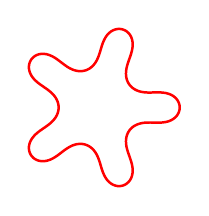
\begin{tikzpicture}[scale=0.45]

  \begin{axis}[
    hide axis,
    axis equal image,
    xmin = -1.42,
    xmax = 1.42,
    ymin = -1.42,
    ymax = 1.42,
    xtick = \empty,
    ytick = \empty,
    title style={align=left},
%    title={\Large $t = 2.99 \times 10^{-2}$ \\ \\ \Large $\nu = 0.38$}
  ]

\addplot[red,line width=2pt] coordinates{
(1.1542e+00,-1.5683e-12)
(1.1521e+00,2.7715e-02)
(1.1455e+00,5.5460e-02)
(1.1342e+00,8.3060e-02)
(1.1178e+00,1.1001e-01)
(1.0958e+00,1.3550e-01)
(1.0683e+00,1.5849e-01)
(1.0358e+00,1.7798e-01)
(9.9887e-01,1.9322e-01)
(9.5866e-01,2.0389e-01)
(9.1618e-01,2.1021e-01)
(8.7237e-01,2.1289e-01)
(8.2802e-01,2.1300e-01)
(7.8370e-01,2.1188e-01)
(7.3992e-01,2.1090e-01)
(6.9718e-01,2.1133e-01)
(6.5612e-01,2.1417e-01)
(6.1746e-01,2.2002e-01)
(5.8201e-01,2.2898e-01)
(5.5047e-01,2.4064e-01)
(5.2334e-01,2.5420e-01)
(5.0081e-01,2.6862e-01)
(4.8274e-01,2.8284e-01)
(4.6868e-01,2.9600e-01)
(4.5795e-01,3.0761e-01)
(4.4962e-01,3.1777e-01)
(4.4254e-01,3.2742e-01)
(4.3553e-01,3.3808e-01)
(4.2794e-01,3.5124e-01)
(4.1981e-01,3.6790e-01)
(4.1176e-01,3.8863e-01)
(4.0468e-01,4.1366e-01)
(3.9964e-01,4.4286e-01)
(3.9760e-01,4.7578e-01)
(3.9926e-01,5.1176e-01)
(4.0486e-01,5.4998e-01)
(4.1418e-01,5.8969e-01)
(4.2649e-01,6.3032e-01)
(4.4073e-01,6.7156e-01)
(4.5554e-01,7.1327e-01)
(4.6949e-01,7.5542e-01)
(4.8111e-01,7.9787e-01)
(4.8909e-01,8.4030e-01)
(4.9239e-01,8.8207e-01)
(4.9039e-01,9.2230e-01)
(4.8297e-01,9.5992e-01)
(4.7051e-01,9.9397e-01)
(4.5380e-01,1.0237e+00)
(4.3380e-01,1.0486e+00)
(4.1143e-01,1.0688e+00)
(3.8735e-01,1.0845e+00)
(3.6191e-01,1.0959e+00)
(3.3516e-01,1.1033e+00)
(3.0704e-01,1.1065e+00)
(2.7755e-01,1.1052e+00)
(2.4697e-01,1.0990e+00)
(2.1593e-01,1.0871e+00)
(1.8536e-01,1.0693e+00)
(1.5633e-01,1.0455e+00)
(1.2983e-01,1.0162e+00)
(1.0657e-01,9.8205e-01)
(8.6754e-02,9.4421e-01)
(7.0115e-02,9.0377e-01)
(5.5924e-02,8.6180e-01)
(4.3149e-02,8.1930e-01)
(3.0636e-02,7.7718e-01)
(1.7298e-02,7.3631e-01)
(2.3040e-03,6.9759e-01)
(-1.4778e-02,6.6193e-01)
(-3.3895e-02,6.3012e-01)
(-5.4525e-02,6.0278e-01)
(-7.5796e-02,5.8022e-01)
(-9.6673e-02,5.6235e-01)
(-1.1616e-01,5.4877e-01)
(-1.3351e-01,5.3883e-01)
(-1.4836e-01,5.3174e-01)
(-1.6095e-01,5.2666e-01)
(-1.7236e-01,5.2276e-01)
(-1.8433e-01,5.1934e-01)
(-1.9858e-01,5.1613e-01)
(-2.1619e-01,5.1339e-01)
(-2.3762e-01,5.1180e-01)
(-2.6288e-01,5.1228e-01)
(-2.9158e-01,5.1579e-01)
(-3.2307e-01,5.2317e-01)
(-3.5650e-01,5.3496e-01)
(-3.9099e-01,5.5123e-01)
(-4.2586e-01,5.7162e-01)
(-4.6072e-01,5.9535e-01)
(-4.9553e-01,6.2132e-01)
(-5.3053e-01,6.4828e-01)
(-5.6614e-01,6.7481e-01)
(-6.0270e-01,6.9952e-01)
(-6.4038e-01,7.2102e-01)
(-6.7896e-01,7.3808e-01)
(-7.1787e-01,7.4976e-01)
(-7.5619e-01,7.5553e-01)
(-7.9288e-01,7.5536e-01)
(-8.2692e-01,7.4966e-01)
(-8.5758e-01,7.3921e-01)
(-8.8447e-01,7.2485e-01)
(-9.0755e-01,7.0735e-01)
(-9.2697e-01,6.8718e-01)
(-9.4291e-01,6.6451e-01)
(-9.5538e-01,6.3929e-01)
(-9.6411e-01,6.1140e-01)
(-9.6854e-01,5.8087e-01)
(-9.6795e-01,5.4807e-01)
(-9.6166e-01,5.1369e-01)
(-9.4925e-01,4.7872e-01)
(-9.3072e-01,4.4424e-01)
(-9.0651e-01,4.1119e-01)
(-8.7748e-01,3.8021e-01)
(-8.4475e-01,3.5146e-01)
(-8.0956e-01,3.2467e-01)
(-7.7318e-01,2.9922e-01)
(-7.3683e-01,2.7429e-01)
(-7.0170e-01,2.4911e-01)
(-6.6892e-01,2.2309e-01)
(-6.3950e-01,1.9602e-01)
(-6.1425e-01,1.6811e-01)
(-5.9367e-01,1.3999e-01)
(-5.7786e-01,1.1254e-01)
(-5.6649e-01,8.6721e-02)
(-5.5894e-01,6.3407e-02)
(-5.5435e-01,4.3180e-02)
(-5.5187e-01,2.6233e-02)
(-5.5074e-01,1.2209e-02)
(-5.5043e-01,1.8275e-12)
(-5.5074e-01,-1.2209e-02)
(-5.5187e-01,-2.6233e-02)
(-5.5435e-01,-4.3180e-02)
(-5.5894e-01,-6.3407e-02)
(-5.6649e-01,-8.6721e-02)
(-5.7786e-01,-1.1254e-01)
(-5.9367e-01,-1.3999e-01)
(-6.1425e-01,-1.6811e-01)
(-6.3950e-01,-1.9602e-01)
(-6.6892e-01,-2.2309e-01)
(-7.0170e-01,-2.4911e-01)
(-7.3683e-01,-2.7429e-01)
(-7.7318e-01,-2.9922e-01)
(-8.0956e-01,-3.2467e-01)
(-8.4475e-01,-3.5146e-01)
(-8.7748e-01,-3.8021e-01)
(-9.0651e-01,-4.1119e-01)
(-9.3072e-01,-4.4424e-01)
(-9.4925e-01,-4.7872e-01)
(-9.6166e-01,-5.1369e-01)
(-9.6795e-01,-5.4807e-01)
(-9.6854e-01,-5.8087e-01)
(-9.6411e-01,-6.1140e-01)
(-9.5538e-01,-6.3929e-01)
(-9.4291e-01,-6.6451e-01)
(-9.2697e-01,-6.8718e-01)
(-9.0755e-01,-7.0735e-01)
(-8.8447e-01,-7.2485e-01)
(-8.5758e-01,-7.3921e-01)
(-8.2692e-01,-7.4966e-01)
(-7.9288e-01,-7.5536e-01)
(-7.5619e-01,-7.5553e-01)
(-7.1787e-01,-7.4976e-01)
(-6.7896e-01,-7.3808e-01)
(-6.4038e-01,-7.2102e-01)
(-6.0270e-01,-6.9952e-01)
(-5.6614e-01,-6.7481e-01)
(-5.3053e-01,-6.4828e-01)
(-4.9553e-01,-6.2132e-01)
(-4.6072e-01,-5.9535e-01)
(-4.2586e-01,-5.7162e-01)
(-3.9099e-01,-5.5123e-01)
(-3.5650e-01,-5.3496e-01)
(-3.2307e-01,-5.2317e-01)
(-2.9158e-01,-5.1579e-01)
(-2.6288e-01,-5.1228e-01)
(-2.3762e-01,-5.1180e-01)
(-2.1619e-01,-5.1339e-01)
(-1.9858e-01,-5.1613e-01)
(-1.8433e-01,-5.1934e-01)
(-1.7236e-01,-5.2276e-01)
(-1.6095e-01,-5.2666e-01)
(-1.4836e-01,-5.3174e-01)
(-1.3351e-01,-5.3883e-01)
(-1.1616e-01,-5.4877e-01)
(-9.6673e-02,-5.6235e-01)
(-7.5796e-02,-5.8022e-01)
(-5.4525e-02,-6.0278e-01)
(-3.3895e-02,-6.3012e-01)
(-1.4778e-02,-6.6193e-01)
(2.3040e-03,-6.9759e-01)
(1.7298e-02,-7.3631e-01)
(3.0636e-02,-7.7718e-01)
(4.3149e-02,-8.1930e-01)
(5.5924e-02,-8.6180e-01)
(7.0115e-02,-9.0377e-01)
(8.6754e-02,-9.4421e-01)
(1.0657e-01,-9.8205e-01)
(1.2983e-01,-1.0162e+00)
(1.5633e-01,-1.0455e+00)
(1.8536e-01,-1.0693e+00)
(2.1593e-01,-1.0871e+00)
(2.4697e-01,-1.0990e+00)
(2.7755e-01,-1.1052e+00)
(3.0704e-01,-1.1065e+00)
(3.3516e-01,-1.1033e+00)
(3.6191e-01,-1.0959e+00)
(3.8735e-01,-1.0845e+00)
(4.1143e-01,-1.0688e+00)
(4.3380e-01,-1.0486e+00)
(4.5380e-01,-1.0237e+00)
(4.7051e-01,-9.9397e-01)
(4.8297e-01,-9.5992e-01)
(4.9039e-01,-9.2230e-01)
(4.9239e-01,-8.8207e-01)
(4.8909e-01,-8.4030e-01)
(4.8111e-01,-7.9787e-01)
(4.6949e-01,-7.5542e-01)
(4.5554e-01,-7.1327e-01)
(4.4073e-01,-6.7156e-01)
(4.2649e-01,-6.3032e-01)
(4.1418e-01,-5.8969e-01)
(4.0486e-01,-5.4998e-01)
(3.9926e-01,-5.1176e-01)
(3.9760e-01,-4.7578e-01)
(3.9964e-01,-4.4286e-01)
(4.0468e-01,-4.1366e-01)
(4.1176e-01,-3.8863e-01)
(4.1981e-01,-3.6790e-01)
(4.2794e-01,-3.5124e-01)
(4.3553e-01,-3.3808e-01)
(4.4254e-01,-3.2742e-01)
(4.4962e-01,-3.1777e-01)
(4.5795e-01,-3.0761e-01)
(4.6868e-01,-2.9600e-01)
(4.8274e-01,-2.8284e-01)
(5.0081e-01,-2.6862e-01)
(5.2334e-01,-2.5420e-01)
(5.5047e-01,-2.4064e-01)
(5.8201e-01,-2.2898e-01)
(6.1746e-01,-2.2002e-01)
(6.5612e-01,-2.1417e-01)
(6.9718e-01,-2.1133e-01)
(7.3992e-01,-2.1090e-01)
(7.8370e-01,-2.1188e-01)
(8.2802e-01,-2.1300e-01)
(8.7237e-01,-2.1289e-01)
(9.1618e-01,-2.1021e-01)
(9.5866e-01,-2.0389e-01)
(9.9887e-01,-1.9322e-01)
(1.0358e+00,-1.7798e-01)
(1.0683e+00,-1.5849e-01)
(1.0958e+00,-1.3550e-01)
(1.1178e+00,-1.1001e-01)
(1.1342e+00,-8.3060e-02)
(1.1455e+00,-5.5460e-02)
(1.1521e+00,-2.7715e-02)
(1.1542e+00,-1.5683e-12)
};


\end{axis}

\end{tikzpicture}

    \quad
    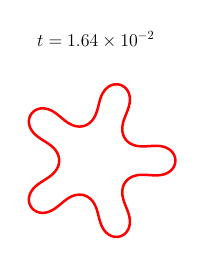
\begin{tikzpicture}[scale=0.45]

  \begin{axis}[
    hide axis,
    axis equal image,
    xmin = -2.1,
    xmax = 2.1,
    ymin = -2.1,
    ymax = 2.1,
    xtick = \empty,
    ytick = \empty,
    title style={align=left},
    title={\Large $t = 1.64 \times 10^{-2}$}
  ]

\addplot[red,line width=2pt] coordinates{
(1.6571e+00,-2.4995e-13)
(1.6540e+00,4.0568e-02)
(1.6446e+00,8.1200e-02)
(1.6282e+00,1.2166e-01)
(1.6043e+00,1.6121e-01)
(1.5722e+00,1.9863e-01)
(1.5321e+00,2.3234e-01)
(1.4844e+00,2.6078e-01)
(1.4303e+00,2.8269e-01)
(1.3712e+00,2.9752e-01)
(1.3088e+00,3.0550e-01)
(1.2447e+00,3.0765e-01)
(1.1798e+00,3.0562e-01)
(1.1150e+00,3.0146e-01)
(1.0511e+00,2.9730e-01)
(9.8855e-01,2.9516e-01)
(9.2832e-01,2.9667e-01)
(8.7143e-01,3.0283e-01)
(8.1907e-01,3.1391e-01)
(7.7235e-01,3.2939e-01)
(7.3210e-01,3.4809e-01)
(6.9865e-01,3.6843e-01)
(6.7184e-01,3.8879e-01)
(6.5103e-01,4.0781e-01)
(6.3518e-01,4.2470e-01)
(6.2292e-01,4.3956e-01)
(6.1255e-01,4.5367e-01)
(6.0232e-01,4.6933e-01)
(5.9132e-01,4.8869e-01)
(5.7970e-01,5.1321e-01)
(5.6840e-01,5.4374e-01)
(5.5884e-01,5.8058e-01)
(5.5264e-01,6.2350e-01)
(5.5125e-01,6.7177e-01)
(5.5567e-01,7.2429e-01)
(5.6620e-01,7.7984e-01)
(5.8238e-01,8.3730e-01)
(6.0302e-01,8.9592e-01)
(6.2643e-01,9.5532e-01)
(6.5053e-01,1.0155e+00)
(6.7308e-01,1.0764e+00)
(6.9187e-01,1.1380e+00)
(7.0491e-01,1.1998e+00)
(7.1065e-01,1.2609e+00)
(7.0821e-01,1.3198e+00)
(6.9750e-01,1.3749e+00)
(6.7921e-01,1.4247e+00)
(6.5461e-01,1.4681e+00)
(6.2519e-01,1.5045e+00)
(5.9232e-01,1.5339e+00)
(5.5701e-01,1.5567e+00)
(5.1976e-01,1.5734e+00)
(4.8061e-01,1.5842e+00)
(4.3946e-01,1.5890e+00)
(3.9629e-01,1.5873e+00)
(3.5151e-01,1.5783e+00)
(3.0601e-01,1.5611e+00)
(2.6120e-01,1.5352e+00)
(2.1875e-01,1.5003e+00)
(1.8023e-01,1.4572e+00)
(1.4679e-01,1.4068e+00)
(1.1886e-01,1.3509e+00)
(9.6059e-02,1.2911e+00)
(7.7305e-02,1.2290e+00)
(6.0987e-02,1.1662e+00)
(4.5272e-02,1.1038e+00)
(2.8403e-02,1.0432e+00)
(8.9895e-03,9.8560e-01)
(-1.3754e-02,9.3237e-01)
(-3.9864e-02,8.8474e-01)
(-6.8632e-02,8.4370e-01)
(-9.8765e-02,8.0976e-01)
(-1.2869e-01,7.8288e-01)
(-1.5685e-01,7.6249e-01)
(-1.8205e-01,7.4761e-01)
(-2.0372e-01,7.3704e-01)
(-2.2214e-01,7.2952e-01)
(-2.3883e-01,7.2379e-01)
(-2.5638e-01,7.1883e-01)
(-2.7730e-01,7.1424e-01)
(-3.0312e-01,7.1049e-01)
(-3.3453e-01,7.0863e-01)
(-3.7147e-01,7.1008e-01)
(-4.1334e-01,7.1633e-01)
(-4.5905e-01,7.2861e-01)
(-5.0730e-01,7.4766e-01)
(-5.5676e-01,7.7353e-01)
(-6.0644e-01,8.0557e-01)
(-6.5587e-01,8.4253e-01)
(-7.0512e-01,8.8272e-01)
(-7.5471e-01,9.2421e-01)
(-8.0539e-01,9.6491e-01)
(-8.5779e-01,1.0027e+00)
(-9.1218e-01,1.0354e+00)
(-9.6824e-01,1.0613e+00)
(-1.0250e+00,1.0789e+00)
(-1.0811e+00,1.0876e+00)
(-1.1348e+00,1.0873e+00)
(-1.1845e+00,1.0788e+00)
(-1.2294e+00,1.0633e+00)
(-1.2686e+00,1.0422e+00)
(-1.3023e+00,1.0164e+00)
(-1.3307e+00,9.8687e-01)
(-1.3541e+00,9.5370e-01)
(-1.3724e+00,9.1682e-01)
(-1.3853e+00,8.7603e-01)
(-1.3920e+00,8.3139e-01)
(-1.3913e+00,7.8337e-01)
(-1.3822e+00,7.3304e-01)
(-1.3640e+00,6.8186e-01)
(-1.3367e+00,6.3152e-01)
(-1.3007e+00,5.8355e-01)
(-1.2574e+00,5.3896e-01)
(-1.2085e+00,4.9808e-01)
(-1.1558e+00,4.6051e-01)
(-1.1012e+00,4.2525e-01)
(-1.0466e+00,3.9099e-01)
(-9.9359e-01,3.5642e-01)
(-9.4396e-01,3.2051e-01)
(-8.9923e-01,2.8279e-01)
(-8.6065e-01,2.4347e-01)
(-8.2907e-01,2.0343e-01)
(-8.0469e-01,1.6398e-01)
(-7.8711e-01,1.2663e-01)
(-7.7539e-01,9.2723e-02)
(-7.6827e-01,6.3215e-02)
(-7.6441e-01,3.8427e-02)
(-7.6264e-01,1.7877e-02)
(-7.6216e-01,-1.0277e-13)
(-7.6264e-01,-1.7877e-02)
(-7.6441e-01,-3.8427e-02)
(-7.6827e-01,-6.3215e-02)
(-7.7539e-01,-9.2723e-02)
(-7.8711e-01,-1.2663e-01)
(-8.0469e-01,-1.6398e-01)
(-8.2907e-01,-2.0343e-01)
(-8.6065e-01,-2.4347e-01)
(-8.9923e-01,-2.8279e-01)
(-9.4396e-01,-3.2051e-01)
(-9.9359e-01,-3.5642e-01)
(-1.0466e+00,-3.9099e-01)
(-1.1012e+00,-4.2525e-01)
(-1.1558e+00,-4.6051e-01)
(-1.2085e+00,-4.9808e-01)
(-1.2574e+00,-5.3896e-01)
(-1.3007e+00,-5.8355e-01)
(-1.3367e+00,-6.3152e-01)
(-1.3640e+00,-6.8186e-01)
(-1.3822e+00,-7.3304e-01)
(-1.3913e+00,-7.8337e-01)
(-1.3920e+00,-8.3139e-01)
(-1.3853e+00,-8.7603e-01)
(-1.3724e+00,-9.1682e-01)
(-1.3541e+00,-9.5370e-01)
(-1.3307e+00,-9.8687e-01)
(-1.3023e+00,-1.0164e+00)
(-1.2686e+00,-1.0422e+00)
(-1.2294e+00,-1.0633e+00)
(-1.1845e+00,-1.0788e+00)
(-1.1348e+00,-1.0873e+00)
(-1.0811e+00,-1.0876e+00)
(-1.0250e+00,-1.0789e+00)
(-9.6824e-01,-1.0613e+00)
(-9.1218e-01,-1.0354e+00)
(-8.5779e-01,-1.0027e+00)
(-8.0539e-01,-9.6491e-01)
(-7.5471e-01,-9.2421e-01)
(-7.0512e-01,-8.8272e-01)
(-6.5587e-01,-8.4253e-01)
(-6.0644e-01,-8.0557e-01)
(-5.5676e-01,-7.7353e-01)
(-5.0730e-01,-7.4766e-01)
(-4.5905e-01,-7.2861e-01)
(-4.1334e-01,-7.1633e-01)
(-3.7147e-01,-7.1008e-01)
(-3.3453e-01,-7.0863e-01)
(-3.0312e-01,-7.1049e-01)
(-2.7730e-01,-7.1424e-01)
(-2.5638e-01,-7.1883e-01)
(-2.3883e-01,-7.2379e-01)
(-2.2214e-01,-7.2952e-01)
(-2.0372e-01,-7.3704e-01)
(-1.8205e-01,-7.4761e-01)
(-1.5685e-01,-7.6249e-01)
(-1.2869e-01,-7.8288e-01)
(-9.8765e-02,-8.0976e-01)
(-6.8632e-02,-8.4370e-01)
(-3.9864e-02,-8.8474e-01)
(-1.3754e-02,-9.3237e-01)
(8.9895e-03,-9.8560e-01)
(2.8403e-02,-1.0432e+00)
(4.5272e-02,-1.1038e+00)
(6.0987e-02,-1.1662e+00)
(7.7305e-02,-1.2290e+00)
(9.6059e-02,-1.2911e+00)
(1.1886e-01,-1.3509e+00)
(1.4679e-01,-1.4068e+00)
(1.8023e-01,-1.4572e+00)
(2.1875e-01,-1.5003e+00)
(2.6120e-01,-1.5352e+00)
(3.0601e-01,-1.5611e+00)
(3.5151e-01,-1.5783e+00)
(3.9629e-01,-1.5873e+00)
(4.3946e-01,-1.5890e+00)
(4.8061e-01,-1.5842e+00)
(5.1976e-01,-1.5734e+00)
(5.5701e-01,-1.5567e+00)
(5.9232e-01,-1.5339e+00)
(6.2519e-01,-1.5045e+00)
(6.5461e-01,-1.4681e+00)
(6.7921e-01,-1.4247e+00)
(6.9750e-01,-1.3749e+00)
(7.0821e-01,-1.3198e+00)
(7.1065e-01,-1.2609e+00)
(7.0491e-01,-1.1998e+00)
(6.9187e-01,-1.1380e+00)
(6.7308e-01,-1.0764e+00)
(6.5053e-01,-1.0155e+00)
(6.2643e-01,-9.5532e-01)
(6.0302e-01,-8.9592e-01)
(5.8238e-01,-8.3730e-01)
(5.6620e-01,-7.7984e-01)
(5.5567e-01,-7.2429e-01)
(5.5125e-01,-6.7177e-01)
(5.5264e-01,-6.2350e-01)
(5.5884e-01,-5.8058e-01)
(5.6840e-01,-5.4374e-01)
(5.7970e-01,-5.1321e-01)
(5.9132e-01,-4.8869e-01)
(6.0232e-01,-4.6933e-01)
(6.1255e-01,-4.5367e-01)
(6.2292e-01,-4.3956e-01)
(6.3518e-01,-4.2470e-01)
(6.5103e-01,-4.0781e-01)
(6.7184e-01,-3.8879e-01)
(6.9865e-01,-3.6843e-01)
(7.3210e-01,-3.4809e-01)
(7.7235e-01,-3.2939e-01)
(8.1907e-01,-3.1391e-01)
(8.7143e-01,-3.0283e-01)
(9.2832e-01,-2.9667e-01)
(9.8855e-01,-2.9516e-01)
(1.0511e+00,-2.9730e-01)
(1.1150e+00,-3.0146e-01)
(1.1798e+00,-3.0562e-01)
(1.2447e+00,-3.0765e-01)
(1.3088e+00,-3.0550e-01)
(1.3712e+00,-2.9752e-01)
(1.4303e+00,-2.8269e-01)
(1.4844e+00,-2.6078e-01)
(1.5321e+00,-2.3234e-01)
(1.5722e+00,-1.9863e-01)
(1.6043e+00,-1.6121e-01)
(1.6282e+00,-1.2166e-01)
(1.6446e+00,-8.1200e-02)
(1.6540e+00,-4.0568e-02)
(1.6571e+00,-2.4995e-13)
};



\end{axis}

\end{tikzpicture}

    \quad
    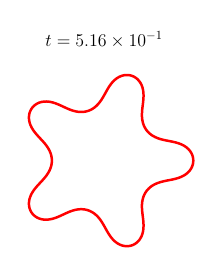
\begin{tikzpicture}[scale=0.45]

  \begin{axis}[
    hide axis,
    axis equal image,
    xmin = -2.1,
    xmax = 2.1,
    ymin = -2.1,
    ymax = 2.1,
    xtick = \empty,
    ytick = \empty,
    title style={align=left},
    title={\Large $t = 5.16 \times 10^{-1}$}
  ]

\addplot[red,line width=2pt] coordinates{
(1.8573e+00,-9.0339e-12)
(1.8547e+00,4.0614e-02)
(1.8468e+00,8.1577e-02)
(1.8329e+00,1.2298e-01)
(1.8125e+00,1.6450e-01)
(1.7849e+00,2.0534e-01)
(1.7499e+00,2.4438e-01)
(1.7076e+00,2.8039e-01)
(1.6587e+00,3.1229e-01)
(1.6042e+00,3.3941e-01)
(1.5454e+00,3.6165e-01)
(1.4837e+00,3.7953e-01)
(1.4204e+00,3.9408e-01)
(1.3568e+00,4.0669e-01)
(1.2938e+00,4.1888e-01)
(1.2327e+00,4.3205e-01)
(1.1744e+00,4.4730e-01)
(1.1200e+00,4.6519e-01)
(1.0706e+00,4.8573e-01)
(1.0269e+00,5.0836e-01)
(9.8935e-01,5.3209e-01)
(9.5812e-01,5.5570e-01)
(9.3291e-01,5.7802e-01)
(9.1310e-01,5.9809e-01)
(8.9780e-01,6.1548e-01)
(8.8578e-01,6.3053e-01)
(8.7542e-01,6.4466e-01)
(8.6500e-01,6.6019e-01)
(8.5345e-01,6.7922e-01)
(8.4067e-01,7.0316e-01)
(8.2726e-01,7.3284e-01)
(8.1423e-01,7.6861e-01)
(8.0279e-01,8.1045e-01)
(7.9411e-01,8.5796e-01)
(7.8906e-01,9.1044e-01)
(7.8804e-01,9.6697e-01)
(7.9086e-01,1.0266e+00)
(7.9675e-01,1.0885e+00)
(8.0444e-01,1.1519e+00)
(8.1229e-01,1.2162e+00)
(8.1853e-01,1.2808e+00)
(8.2145e-01,1.3452e+00)
(8.1957e-01,1.4084e+00)
(8.1186e-01,1.4692e+00)
(7.9790e-01,1.5265e+00)
(7.7786e-01,1.5789e+00)
(7.5249e-01,1.6256e+00)
(7.2287e-01,1.6657e+00)
(6.9018e-01,1.6993e+00)
(6.5541e-01,1.7264e+00)
(6.1917e-01,1.7478e+00)
(5.8162e-01,1.7638e+00)
(5.4255e-01,1.7749e+00)
(5.0156e-01,1.7810e+00)
(4.5835e-01,1.7817e+00)
(4.1296e-01,1.7765e+00)
(3.6585e-01,1.7643e+00)
(3.1792e-01,1.7447e+00)
(2.7038e-01,1.7172e+00)
(2.2445e-01,1.6819e+00)
(1.8119e-01,1.6397e+00)
(1.4119e-01,1.5917e+00)
(1.0450e-01,1.5392e+00)
(7.0641e-02,1.4839e+00)
(3.8719e-02,1.4274e+00)
(7.6439e-03,1.3711e+00)
(-2.3635e-02,1.3165e+00)
(-5.5892e-02,1.2650e+00)
(-8.9454e-02,1.2178e+00)
(-1.2412e-01,1.1760e+00)
(-1.5918e-01,1.1401e+00)
(-1.9361e-01,1.1105e+00)
(-2.2623e-01,1.0870e+00)
(-2.5593e-01,1.0689e+00)
(-2.8193e-01,1.0555e+00)
(-3.0396e-01,1.0457e+00)
(-3.2253e-01,1.0385e+00)
(-3.3924e-01,1.0328e+00)
(-3.5674e-01,1.0277e+00)
(-3.7754e-01,1.0226e+00)
(-4.0318e-01,1.0177e+00)
(-4.3440e-01,1.0138e+00)
(-4.7133e-01,1.0119e+00)
(-5.1365e-01,1.0132e+00)
(-5.6068e-01,1.0187e+00)
(-6.1151e-01,1.0291e+00)
(-6.6515e-01,1.0446e+00)
(-7.2070e-01,1.0648e+00)
(-7.7752e-01,1.0890e+00)
(-8.3526e-01,1.1155e+00)
(-8.9383e-01,1.1429e+00)
(-9.5324e-01,1.1693e+00)
(-1.0134e+00,1.1928e+00)
(-1.0741e+00,1.2116e+00)
(-1.1345e+00,1.2244e+00)
(-1.1936e+00,1.2303e+00)
(-1.2504e+00,1.2289e+00)
(-1.3034e+00,1.2204e+00)
(-1.3518e+00,1.2058e+00)
(-1.3949e+00,1.1860e+00)
(-1.4325e+00,1.1620e+00)
(-1.4650e+00,1.1348e+00)
(-1.4927e+00,1.1046e+00)
(-1.5161e+00,1.0715e+00)
(-1.5355e+00,1.0351e+00)
(-1.5505e+00,9.9499e-01)
(-1.5606e+00,9.5098e-01)
(-1.5649e+00,9.0314e-01)
(-1.5624e+00,8.5203e-01)
(-1.5525e+00,7.9862e-01)
(-1.5347e+00,7.4413e-01)
(-1.5094e+00,6.8978e-01)
(-1.4773e+00,6.3657e-01)
(-1.4397e+00,5.8510e-01)
(-1.3981e+00,5.3547e-01)
(-1.3544e+00,4.8738e-01)
(-1.3103e+00,4.4029e-01)
(-1.2676e+00,3.9364e-01)
(-1.2278e+00,3.4705e-01)
(-1.1923e+00,3.0051e-01)
(-1.1621e+00,2.5444e-01)
(-1.1377e+00,2.0964e-01)
(-1.1191e+00,1.6716e-01)
(-1.1058e+00,1.2807e-01)
(-1.0970e+00,9.3280e-02)
(-1.0917e+00,6.3390e-02)
(-1.0888e+00,3.8466e-02)
(-1.0875e+00,1.7880e-02)
(-1.0871e+00,1.1759e-11)
(-1.0875e+00,-1.7880e-02)
(-1.0888e+00,-3.8466e-02)
(-1.0917e+00,-6.3390e-02)
(-1.0970e+00,-9.3280e-02)
(-1.1058e+00,-1.2807e-01)
(-1.1191e+00,-1.6716e-01)
(-1.1377e+00,-2.0964e-01)
(-1.1621e+00,-2.5444e-01)
(-1.1923e+00,-3.0051e-01)
(-1.2278e+00,-3.4705e-01)
(-1.2676e+00,-3.9364e-01)
(-1.3103e+00,-4.4029e-01)
(-1.3544e+00,-4.8738e-01)
(-1.3981e+00,-5.3547e-01)
(-1.4397e+00,-5.8510e-01)
(-1.4773e+00,-6.3657e-01)
(-1.5094e+00,-6.8978e-01)
(-1.5347e+00,-7.4413e-01)
(-1.5525e+00,-7.9862e-01)
(-1.5624e+00,-8.5203e-01)
(-1.5649e+00,-9.0314e-01)
(-1.5606e+00,-9.5098e-01)
(-1.5505e+00,-9.9499e-01)
(-1.5355e+00,-1.0351e+00)
(-1.5161e+00,-1.0715e+00)
(-1.4927e+00,-1.1046e+00)
(-1.4650e+00,-1.1348e+00)
(-1.4325e+00,-1.1620e+00)
(-1.3949e+00,-1.1860e+00)
(-1.3518e+00,-1.2058e+00)
(-1.3034e+00,-1.2204e+00)
(-1.2504e+00,-1.2289e+00)
(-1.1936e+00,-1.2303e+00)
(-1.1345e+00,-1.2244e+00)
(-1.0741e+00,-1.2116e+00)
(-1.0134e+00,-1.1928e+00)
(-9.5324e-01,-1.1693e+00)
(-8.9383e-01,-1.1429e+00)
(-8.3526e-01,-1.1155e+00)
(-7.7752e-01,-1.0890e+00)
(-7.2070e-01,-1.0648e+00)
(-6.6515e-01,-1.0446e+00)
(-6.1151e-01,-1.0291e+00)
(-5.6068e-01,-1.0187e+00)
(-5.1365e-01,-1.0132e+00)
(-4.7133e-01,-1.0119e+00)
(-4.3440e-01,-1.0138e+00)
(-4.0318e-01,-1.0177e+00)
(-3.7754e-01,-1.0226e+00)
(-3.5674e-01,-1.0277e+00)
(-3.3924e-01,-1.0328e+00)
(-3.2253e-01,-1.0385e+00)
(-3.0396e-01,-1.0457e+00)
(-2.8193e-01,-1.0555e+00)
(-2.5593e-01,-1.0689e+00)
(-2.2623e-01,-1.0870e+00)
(-1.9361e-01,-1.1105e+00)
(-1.5918e-01,-1.1401e+00)
(-1.2412e-01,-1.1760e+00)
(-8.9454e-02,-1.2178e+00)
(-5.5892e-02,-1.2650e+00)
(-2.3635e-02,-1.3165e+00)
(7.6439e-03,-1.3711e+00)
(3.8719e-02,-1.4274e+00)
(7.0641e-02,-1.4839e+00)
(1.0450e-01,-1.5392e+00)
(1.4119e-01,-1.5917e+00)
(1.8119e-01,-1.6397e+00)
(2.2445e-01,-1.6819e+00)
(2.7038e-01,-1.7172e+00)
(3.1792e-01,-1.7447e+00)
(3.6585e-01,-1.7643e+00)
(4.1296e-01,-1.7765e+00)
(4.5835e-01,-1.7817e+00)
(5.0156e-01,-1.7810e+00)
(5.4255e-01,-1.7749e+00)
(5.8162e-01,-1.7638e+00)
(6.1917e-01,-1.7478e+00)
(6.5541e-01,-1.7264e+00)
(6.9018e-01,-1.6993e+00)
(7.2287e-01,-1.6657e+00)
(7.5249e-01,-1.6256e+00)
(7.7786e-01,-1.5789e+00)
(7.9790e-01,-1.5265e+00)
(8.1186e-01,-1.4692e+00)
(8.1957e-01,-1.4084e+00)
(8.2145e-01,-1.3452e+00)
(8.1853e-01,-1.2808e+00)
(8.1229e-01,-1.2162e+00)
(8.0444e-01,-1.1519e+00)
(7.9675e-01,-1.0885e+00)
(7.9086e-01,-1.0266e+00)
(7.8804e-01,-9.6697e-01)
(7.8906e-01,-9.1044e-01)
(7.9411e-01,-8.5796e-01)
(8.0279e-01,-8.1045e-01)
(8.1423e-01,-7.6861e-01)
(8.2726e-01,-7.3284e-01)
(8.4067e-01,-7.0316e-01)
(8.5345e-01,-6.7922e-01)
(8.6500e-01,-6.6019e-01)
(8.7542e-01,-6.4466e-01)
(8.8578e-01,-6.3053e-01)
(8.9780e-01,-6.1548e-01)
(9.1310e-01,-5.9809e-01)
(9.3291e-01,-5.7802e-01)
(9.5812e-01,-5.5570e-01)
(9.8935e-01,-5.3209e-01)
(1.0269e+00,-5.0836e-01)
(1.0706e+00,-4.8573e-01)
(1.1200e+00,-4.6519e-01)
(1.1744e+00,-4.4730e-01)
(1.2327e+00,-4.3205e-01)
(1.2938e+00,-4.1888e-01)
(1.3568e+00,-4.0669e-01)
(1.4204e+00,-3.9408e-01)
(1.4837e+00,-3.7953e-01)
(1.5454e+00,-3.6165e-01)
(1.6042e+00,-3.3941e-01)
(1.6587e+00,-3.1229e-01)
(1.7076e+00,-2.8039e-01)
(1.7499e+00,-2.4438e-01)
(1.7849e+00,-2.0534e-01)
(1.8125e+00,-1.6450e-01)
(1.8329e+00,-1.2298e-01)
(1.8468e+00,-8.1577e-02)
(1.8547e+00,-4.0614e-02)
(1.8573e+00,-9.0339e-12)
};



\end{axis}

\end{tikzpicture}

    \quad
    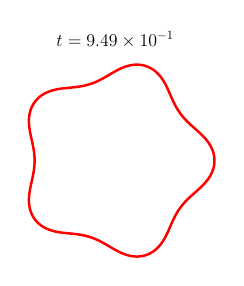
\begin{tikzpicture}[scale=0.45]

  \begin{axis}[
    hide axis,
    axis equal image,
    xmin = -2.1,
    xmax = 2.1,
    ymin = -2.1,
    ymax = 2.1,
    xtick = \empty,
    ytick = \empty,
    title style={align=left},
    title={\Large $t = 9.49 \times 10^{-1}$}
  ]

\addplot[red,line width=2pt] coordinates{
(2.0699e+00,-5.6473e-11)
(2.0685e+00,4.0691e-02)
(2.0641e+00,8.2211e-02)
(2.0564e+00,1.2521e-01)
(2.0450e+00,1.7005e-01)
(2.0292e+00,2.1674e-01)
(2.0085e+00,2.6499e-01)
(1.9828e+00,3.1424e-01)
(1.9519e+00,3.6386e-01)
(1.9161e+00,4.1317e-01)
(1.8760e+00,4.6160e-01)
(1.8324e+00,5.0875e-01)
(1.7863e+00,5.5443e-01)
(1.7387e+00,5.9859e-01)
(1.6909e+00,6.4131e-01)
(1.6440e+00,6.8270e-01)
(1.5990e+00,7.2276e-01)
(1.5568e+00,7.6141e-01)
(1.5181e+00,7.9839e-01)
(1.4833e+00,8.3329e-01)
(1.4529e+00,8.6561e-01)
(1.4268e+00,8.9485e-01)
(1.4051e+00,9.2056e-01)
(1.3873e+00,9.4249e-01)
(1.3731e+00,9.6079e-01)
(1.3616e+00,9.7620e-01)
(1.3513e+00,9.9036e-01)
(1.3405e+00,1.0056e+00)
(1.3279e+00,1.0240e+00)
(1.3130e+00,1.0467e+00)
(1.2957e+00,1.0743e+00)
(1.2763e+00,1.1071e+00)
(1.2553e+00,1.1450e+00)
(1.2330e+00,1.1879e+00)
(1.2099e+00,1.2353e+00)
(1.1863e+00,1.2867e+00)
(1.1622e+00,1.3413e+00)
(1.1375e+00,1.3984e+00)
(1.1119e+00,1.4568e+00)
(1.0849e+00,1.5157e+00)
(1.0561e+00,1.5740e+00)
(1.0252e+00,1.6305e+00)
(9.9198e-01,1.6843e+00)
(9.5655e-01,1.7344e+00)
(9.1923e-01,1.7800e+00)
(8.8054e-01,1.8208e+00)
(8.4111e-01,1.8563e+00)
(8.0155e-01,1.8868e+00)
(7.6235e-01,1.9125e+00)
(7.2371e-01,1.9338e+00)
(6.8552e-01,1.9515e+00)
(6.4734e-01,1.9660e+00)
(6.0845e-01,1.9777e+00)
(5.6801e-01,1.9869e+00)
(5.2528e-01,1.9935e+00)
(4.7970e-01,1.9971e+00)
(4.3103e-01,1.9972e+00)
(3.7934e-01,1.9934e+00)
(3.2500e-01,1.9851e+00)
(2.6860e-01,1.9720e+00)
(2.1083e-01,1.9542e+00)
(1.5243e-01,1.9318e+00)
(9.4027e-02,1.9056e+00)
(3.6168e-02,1.8763e+00)
(-2.0752e-02,1.8450e+00)
(-7.6433e-02,1.8129e+00)
(-1.3062e-01,1.7809e+00)
(-1.8303e-01,1.7501e+00)
(-2.3332e-01,1.7214e+00)
(-2.8103e-01,1.6954e+00)
(-3.2564e-01,1.6725e+00)
(-3.6659e-01,1.6529e+00)
(-4.0334e-01,1.6365e+00)
(-4.3548e-01,1.6232e+00)
(-4.6277e-01,1.6126e+00)
(-4.8543e-01,1.6043e+00)
(-5.0424e-01,1.5978e+00)
(-5.2100e-01,1.5923e+00)
(-5.3840e-01,1.5868e+00)
(-5.5893e-01,1.5807e+00)
(-5.8408e-01,1.5737e+00)
(-6.1457e-01,1.5660e+00)
(-6.5062e-01,1.5577e+00)
(-6.9215e-01,1.5494e+00)
(-7.3882e-01,1.5413e+00)
(-7.9018e-01,1.5339e+00)
(-8.4562e-01,1.5272e+00)
(-9.0443e-01,1.5210e+00)
(-9.6588e-01,1.5152e+00)
(-1.0291e+00,1.5090e+00)
(-1.0934e+00,1.5018e+00)
(-1.1578e+00,1.4929e+00)
(-1.2214e+00,1.4815e+00)
(-1.2832e+00,1.4672e+00)
(-1.3424e+00,1.4496e+00)
(-1.3982e+00,1.4288e+00)
(-1.4498e+00,1.4051e+00)
(-1.4967e+00,1.3790e+00)
(-1.5389e+00,1.3511e+00)
(-1.5763e+00,1.3219e+00)
(-1.6094e+00,1.2919e+00)
(-1.6387e+00,1.2612e+00)
(-1.6648e+00,1.2296e+00)
(-1.6884e+00,1.1966e+00)
(-1.7100e+00,1.1615e+00)
(-1.7298e+00,1.1236e+00)
(-1.7478e+00,1.0821e+00)
(-1.7635e+00,1.0367e+00)
(-1.7764e+00,9.8714e-01)
(-1.7860e+00,9.3364e-01)
(-1.7918e+00,8.7660e-01)
(-1.7935e+00,8.1664e-01)
(-1.7911e+00,7.5452e-01)
(-1.7849e+00,6.9105e-01)
(-1.7755e+00,6.2701e-01)
(-1.7637e+00,5.6310e-01)
(-1.7505e+00,4.9997e-01)
(-1.7368e+00,4.3821e-01)
(-1.7236e+00,3.7839e-01)
(-1.7115e+00,3.2111e-01)
(-1.7011e+00,2.6699e-01)
(-1.6927e+00,2.1666e-01)
(-1.6863e+00,1.7071e-01)
(-1.6818e+00,1.2966e-01)
(-1.6788e+00,9.3894e-02)
(-1.6770e+00,6.3583e-02)
(-1.6760e+00,3.8509e-02)
(-1.6755e+00,1.7885e-02)
(-1.6754e+00,-9.7486e-12)
(-1.6755e+00,-1.7885e-02)
(-1.6760e+00,-3.8509e-02)
(-1.6770e+00,-6.3583e-02)
(-1.6788e+00,-9.3894e-02)
(-1.6818e+00,-1.2966e-01)
(-1.6863e+00,-1.7071e-01)
(-1.6927e+00,-2.1666e-01)
(-1.7011e+00,-2.6699e-01)
(-1.7115e+00,-3.2111e-01)
(-1.7236e+00,-3.7839e-01)
(-1.7368e+00,-4.3821e-01)
(-1.7505e+00,-4.9997e-01)
(-1.7637e+00,-5.6310e-01)
(-1.7755e+00,-6.2701e-01)
(-1.7849e+00,-6.9105e-01)
(-1.7911e+00,-7.5452e-01)
(-1.7935e+00,-8.1664e-01)
(-1.7918e+00,-8.7660e-01)
(-1.7860e+00,-9.3364e-01)
(-1.7764e+00,-9.8714e-01)
(-1.7635e+00,-1.0367e+00)
(-1.7478e+00,-1.0821e+00)
(-1.7298e+00,-1.1236e+00)
(-1.7100e+00,-1.1615e+00)
(-1.6884e+00,-1.1966e+00)
(-1.6648e+00,-1.2296e+00)
(-1.6387e+00,-1.2612e+00)
(-1.6094e+00,-1.2919e+00)
(-1.5763e+00,-1.3219e+00)
(-1.5389e+00,-1.3511e+00)
(-1.4967e+00,-1.3790e+00)
(-1.4498e+00,-1.4051e+00)
(-1.3982e+00,-1.4288e+00)
(-1.3424e+00,-1.4496e+00)
(-1.2832e+00,-1.4672e+00)
(-1.2214e+00,-1.4815e+00)
(-1.1578e+00,-1.4929e+00)
(-1.0934e+00,-1.5018e+00)
(-1.0291e+00,-1.5090e+00)
(-9.6588e-01,-1.5152e+00)
(-9.0443e-01,-1.5210e+00)
(-8.4562e-01,-1.5272e+00)
(-7.9018e-01,-1.5339e+00)
(-7.3882e-01,-1.5413e+00)
(-6.9215e-01,-1.5494e+00)
(-6.5062e-01,-1.5577e+00)
(-6.1457e-01,-1.5660e+00)
(-5.8408e-01,-1.5737e+00)
(-5.5893e-01,-1.5807e+00)
(-5.3840e-01,-1.5868e+00)
(-5.2100e-01,-1.5923e+00)
(-5.0424e-01,-1.5978e+00)
(-4.8543e-01,-1.6043e+00)
(-4.6277e-01,-1.6126e+00)
(-4.3548e-01,-1.6232e+00)
(-4.0334e-01,-1.6365e+00)
(-3.6659e-01,-1.6529e+00)
(-3.2564e-01,-1.6725e+00)
(-2.8103e-01,-1.6954e+00)
(-2.3332e-01,-1.7214e+00)
(-1.8303e-01,-1.7501e+00)
(-1.3062e-01,-1.7809e+00)
(-7.6433e-02,-1.8129e+00)
(-2.0752e-02,-1.8450e+00)
(3.6168e-02,-1.8763e+00)
(9.4027e-02,-1.9056e+00)
(1.5243e-01,-1.9318e+00)
(2.1083e-01,-1.9542e+00)
(2.6860e-01,-1.9720e+00)
(3.2500e-01,-1.9851e+00)
(3.7934e-01,-1.9934e+00)
(4.3103e-01,-1.9972e+00)
(4.7970e-01,-1.9971e+00)
(5.2528e-01,-1.9935e+00)
(5.6801e-01,-1.9869e+00)
(6.0845e-01,-1.9777e+00)
(6.4734e-01,-1.9660e+00)
(6.8552e-01,-1.9515e+00)
(7.2371e-01,-1.9338e+00)
(7.6235e-01,-1.9125e+00)
(8.0155e-01,-1.8868e+00)
(8.4111e-01,-1.8563e+00)
(8.8054e-01,-1.8208e+00)
(9.1923e-01,-1.7800e+00)
(9.5655e-01,-1.7344e+00)
(9.9198e-01,-1.6843e+00)
(1.0252e+00,-1.6305e+00)
(1.0561e+00,-1.5740e+00)
(1.0849e+00,-1.5157e+00)
(1.1119e+00,-1.4568e+00)
(1.1375e+00,-1.3984e+00)
(1.1622e+00,-1.3413e+00)
(1.1863e+00,-1.2867e+00)
(1.2099e+00,-1.2353e+00)
(1.2330e+00,-1.1879e+00)
(1.2553e+00,-1.1450e+00)
(1.2763e+00,-1.1071e+00)
(1.2957e+00,-1.0743e+00)
(1.3130e+00,-1.0467e+00)
(1.3279e+00,-1.0240e+00)
(1.3405e+00,-1.0056e+00)
(1.3513e+00,-9.9036e-01)
(1.3616e+00,-9.7620e-01)
(1.3731e+00,-9.6079e-01)
(1.3873e+00,-9.4249e-01)
(1.4051e+00,-9.2056e-01)
(1.4268e+00,-8.9485e-01)
(1.4529e+00,-8.6561e-01)
(1.4833e+00,-8.3329e-01)
(1.5181e+00,-7.9839e-01)
(1.5568e+00,-7.6141e-01)
(1.5990e+00,-7.2276e-01)
(1.6440e+00,-6.8270e-01)
(1.6909e+00,-6.4131e-01)
(1.7387e+00,-5.9859e-01)
(1.7863e+00,-5.5443e-01)
(1.8324e+00,-5.0875e-01)
(1.8760e+00,-4.6160e-01)
(1.9161e+00,-4.1317e-01)
(1.9519e+00,-3.6386e-01)
(1.9828e+00,-3.1424e-01)
(2.0085e+00,-2.6499e-01)
(2.0292e+00,-2.1674e-01)
(2.0450e+00,-1.7005e-01)
(2.0564e+00,-1.2521e-01)
(2.0641e+00,-8.2211e-02)
(2.0685e+00,-4.0691e-02)
(2.0699e+00,-5.6473e-11)
};


\end{axis}

\end{tikzpicture}

    \quad
    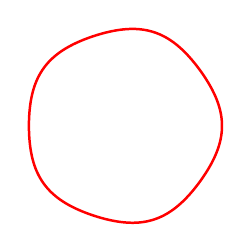
\begin{tikzpicture}[scale=0.45]

  \begin{axis}[
    hide axis,
    axis equal image,
    xmin = -1.42,
    xmax = 1.42,
    ymin = -1.42,
    ymax = 1.42,
    xtick = \empty,
    ytick = \empty,
    title style={align=left},
%    title={\Large $t = 3.17 \times 10^{-1}$ \\ \\ \Large $\nu = 0.99$}
  ]

\addplot[red,line width=2pt] coordinates{
(1.3864e+00,-4.3575e-10)
(1.3860e+00,2.7820e-02)
(1.3847e+00,5.6320e-02)
(1.3823e+00,8.6084e-02)
(1.3788e+00,1.1752e-01)
(1.3739e+00,1.5087e-01)
(1.3674e+00,1.8615e-01)
(1.3591e+00,2.2325e-01)
(1.3488e+00,2.6191e-01)
(1.3367e+00,3.0178e-01)
(1.3226e+00,3.4244e-01)
(1.3068e+00,3.8343e-01)
(1.2894e+00,4.2430e-01)
(1.2707e+00,4.6458e-01)
(1.2512e+00,5.0382e-01)
(1.2311e+00,5.4160e-01)
(1.2109e+00,5.7754e-01)
(1.1911e+00,6.1127e-01)
(1.1719e+00,6.4247e-01)
(1.1539e+00,6.7088e-01)
(1.1372e+00,6.9627e-01)
(1.1223e+00,7.1848e-01)
(1.1093e+00,7.3745e-01)
(1.0982e+00,7.5324e-01)
(1.0891e+00,7.6613e-01)
(1.0814e+00,7.7680e-01)
(1.0744e+00,7.8649e-01)
(1.0668e+00,7.9678e-01)
(1.0578e+00,8.0899e-01)
(1.0466e+00,8.2380e-01)
(1.0331e+00,8.4148e-01)
(1.0171e+00,8.6199e-01)
(9.9861e-01,8.8515e-01)
(9.7765e-01,9.1067e-01)
(9.5434e-01,9.3817e-01)
(9.2882e-01,9.6722e-01)
(9.0126e-01,9.9735e-01)
(8.7187e-01,1.0281e+00)
(8.4088e-01,1.0588e+00)
(8.0857e-01,1.0892e+00)
(7.7524e-01,1.1186e+00)
(7.4124e-01,1.1467e+00)
(7.0693e-01,1.1730e+00)
(6.7270e-01,1.1973e+00)
(6.3895e-01,1.2194e+00)
(6.0603e-01,1.2392e+00)
(5.7424e-01,1.2568e+00)
(5.4378e-01,1.2722e+00)
(5.1469e-01,1.2856e+00)
(4.8689e-01,1.2973e+00)
(4.6005e-01,1.3077e+00)
(4.3370e-01,1.3169e+00)
(4.0721e-01,1.3252e+00)
(3.7993e-01,1.3329e+00)
(3.5125e-01,1.3399e+00)
(3.2068e-01,1.3464e+00)
(2.8790e-01,1.3522e+00)
(2.5280e-01,1.3571e+00)
(2.1539e-01,1.3609e+00)
(1.7586e-01,1.3634e+00)
(1.3451e-01,1.3645e+00)
(9.1724e-02,1.3640e+00)
(4.7970e-02,1.3619e+00)
(3.7546e-03,1.3583e+00)
(-4.0394e-02,1.3532e+00)
(-8.3942e-02,1.3470e+00)
(-1.2636e-01,1.3397e+00)
(-1.6716e-01,1.3318e+00)
(-2.0585e-01,1.3234e+00)
(-2.4200e-01,1.3148e+00)
(-2.7522e-01,1.3064e+00)
(-3.0519e-01,1.2983e+00)
(-3.3165e-01,1.2908e+00)
(-3.5445e-01,1.2841e+00)
(-3.7359e-01,1.2783e+00)
(-3.8931e-01,1.2734e+00)
(-4.0225e-01,1.2693e+00)
(-4.1371e-01,1.2656e+00)
(-4.2554e-01,1.2617e+00)
(-4.3940e-01,1.2571e+00)
(-4.5627e-01,1.2513e+00)
(-4.7656e-01,1.2442e+00)
(-5.0033e-01,1.2356e+00)
(-5.2744e-01,1.2255e+00)
(-5.5761e-01,1.2137e+00)
(-5.9048e-01,1.2004e+00)
(-6.2561e-01,1.1854e+00)
(-6.6249e-01,1.1689e+00)
(-7.0061e-01,1.1507e+00)
(-7.3939e-01,1.1310e+00)
(-7.7827e-01,1.1099e+00)
(-8.1670e-01,1.0876e+00)
(-8.5415e-01,1.0641e+00)
(-8.9013e-01,1.0398e+00)
(-9.2424e-01,1.0148e+00)
(-9.5617e-01,9.8955e-01)
(-9.8569e-01,9.6433e-01)
(-1.0127e+00,9.3942e-01)
(-1.0373e+00,9.1507e-01)
(-1.0595e+00,8.9142e-01)
(-1.0796e+00,8.6848e-01)
(-1.0980e+00,8.4607e-01)
(-1.1151e+00,8.2386e-01)
(-1.1313e+00,8.0137e-01)
(-1.1471e+00,7.7803e-01)
(-1.1627e+00,7.5329e-01)
(-1.1783e+00,7.2664e-01)
(-1.1939e+00,6.9774e-01)
(-1.2095e+00,6.6637e-01)
(-1.2247e+00,6.3247e-01)
(-1.2395e+00,5.9612e-01)
(-1.2535e+00,5.5754e-01)
(-1.2664e+00,5.1703e-01)
(-1.2782e+00,4.7502e-01)
(-1.2887e+00,4.3199e-01)
(-1.2978e+00,3.8847e-01)
(-1.3056e+00,3.4504e-01)
(-1.3121e+00,3.0225e-01)
(-1.3173e+00,2.6068e-01)
(-1.3215e+00,2.2087e-01)
(-1.3247e+00,1.8334e-01)
(-1.3271e+00,1.4853e-01)
(-1.3288e+00,1.1687e-01)
(-1.3299e+00,8.8668e-02)
(-1.3307e+00,6.4158e-02)
(-1.3311e+00,4.3415e-02)
(-1.3314e+00,2.6286e-02)
(-1.3315e+00,1.2214e-02)
(-1.3315e+00,2.3306e-10)
(-1.3315e+00,-1.2214e-02)
(-1.3314e+00,-2.6286e-02)
(-1.3311e+00,-4.3415e-02)
(-1.3307e+00,-6.4158e-02)
(-1.3299e+00,-8.8668e-02)
(-1.3288e+00,-1.1687e-01)
(-1.3271e+00,-1.4853e-01)
(-1.3247e+00,-1.8334e-01)
(-1.3215e+00,-2.2087e-01)
(-1.3173e+00,-2.6068e-01)
(-1.3121e+00,-3.0225e-01)
(-1.3056e+00,-3.4504e-01)
(-1.2978e+00,-3.8847e-01)
(-1.2887e+00,-4.3199e-01)
(-1.2782e+00,-4.7502e-01)
(-1.2664e+00,-5.1703e-01)
(-1.2535e+00,-5.5754e-01)
(-1.2395e+00,-5.9612e-01)
(-1.2247e+00,-6.3247e-01)
(-1.2095e+00,-6.6637e-01)
(-1.1939e+00,-6.9774e-01)
(-1.1783e+00,-7.2664e-01)
(-1.1627e+00,-7.5329e-01)
(-1.1471e+00,-7.7803e-01)
(-1.1313e+00,-8.0137e-01)
(-1.1151e+00,-8.2386e-01)
(-1.0980e+00,-8.4607e-01)
(-1.0796e+00,-8.6848e-01)
(-1.0595e+00,-8.9142e-01)
(-1.0373e+00,-9.1507e-01)
(-1.0127e+00,-9.3942e-01)
(-9.8569e-01,-9.6433e-01)
(-9.5617e-01,-9.8955e-01)
(-9.2424e-01,-1.0148e+00)
(-8.9013e-01,-1.0398e+00)
(-8.5415e-01,-1.0641e+00)
(-8.1670e-01,-1.0876e+00)
(-7.7827e-01,-1.1099e+00)
(-7.3939e-01,-1.1310e+00)
(-7.0061e-01,-1.1507e+00)
(-6.6249e-01,-1.1689e+00)
(-6.2561e-01,-1.1854e+00)
(-5.9048e-01,-1.2004e+00)
(-5.5761e-01,-1.2137e+00)
(-5.2744e-01,-1.2255e+00)
(-5.0033e-01,-1.2356e+00)
(-4.7656e-01,-1.2442e+00)
(-4.5627e-01,-1.2513e+00)
(-4.3940e-01,-1.2571e+00)
(-4.2554e-01,-1.2617e+00)
(-4.1371e-01,-1.2656e+00)
(-4.0225e-01,-1.2693e+00)
(-3.8931e-01,-1.2734e+00)
(-3.7359e-01,-1.2783e+00)
(-3.5445e-01,-1.2841e+00)
(-3.3165e-01,-1.2908e+00)
(-3.0519e-01,-1.2983e+00)
(-2.7522e-01,-1.3064e+00)
(-2.4200e-01,-1.3148e+00)
(-2.0585e-01,-1.3234e+00)
(-1.6716e-01,-1.3318e+00)
(-1.2636e-01,-1.3397e+00)
(-8.3942e-02,-1.3470e+00)
(-4.0394e-02,-1.3532e+00)
(3.7546e-03,-1.3583e+00)
(4.7970e-02,-1.3619e+00)
(9.1724e-02,-1.3640e+00)
(1.3451e-01,-1.3645e+00)
(1.7586e-01,-1.3634e+00)
(2.1539e-01,-1.3609e+00)
(2.5280e-01,-1.3571e+00)
(2.8790e-01,-1.3522e+00)
(3.2068e-01,-1.3464e+00)
(3.5125e-01,-1.3399e+00)
(3.7993e-01,-1.3329e+00)
(4.0721e-01,-1.3252e+00)
(4.3370e-01,-1.3169e+00)
(4.6005e-01,-1.3077e+00)
(4.8689e-01,-1.2973e+00)
(5.1469e-01,-1.2856e+00)
(5.4378e-01,-1.2722e+00)
(5.7424e-01,-1.2568e+00)
(6.0603e-01,-1.2392e+00)
(6.3895e-01,-1.2194e+00)
(6.7270e-01,-1.1973e+00)
(7.0693e-01,-1.1730e+00)
(7.4124e-01,-1.1467e+00)
(7.7524e-01,-1.1186e+00)
(8.0857e-01,-1.0892e+00)
(8.4088e-01,-1.0588e+00)
(8.7187e-01,-1.0281e+00)
(9.0126e-01,-9.9735e-01)
(9.2882e-01,-9.6722e-01)
(9.5434e-01,-9.3817e-01)
(9.7765e-01,-9.1067e-01)
(9.9861e-01,-8.8515e-01)
(1.0171e+00,-8.6199e-01)
(1.0331e+00,-8.4148e-01)
(1.0466e+00,-8.2380e-01)
(1.0578e+00,-8.0899e-01)
(1.0668e+00,-7.9678e-01)
(1.0744e+00,-7.8649e-01)
(1.0814e+00,-7.7680e-01)
(1.0891e+00,-7.6613e-01)
(1.0982e+00,-7.5324e-01)
(1.1093e+00,-7.3745e-01)
(1.1223e+00,-7.1848e-01)
(1.1372e+00,-6.9627e-01)
(1.1539e+00,-6.7088e-01)
(1.1719e+00,-6.4247e-01)
(1.1911e+00,-6.1127e-01)
(1.2109e+00,-5.7754e-01)
(1.2311e+00,-5.4160e-01)
(1.2512e+00,-5.0382e-01)
(1.2707e+00,-4.6458e-01)
(1.2894e+00,-4.2430e-01)
(1.3068e+00,-3.8343e-01)
(1.3226e+00,-3.4244e-01)
(1.3367e+00,-3.0178e-01)
(1.3488e+00,-2.6191e-01)
(1.3591e+00,-2.2325e-01)
(1.3674e+00,-1.8615e-01)
(1.3739e+00,-1.5087e-01)
(1.3788e+00,-1.1752e-01)
(1.3823e+00,-8.6084e-02)
(1.3847e+00,-5.6320e-02)
(1.3860e+00,-2.7820e-02)
(1.3864e+00,-4.3575e-10)
};



\end{axis}

\end{tikzpicture}

    \fi
  \caption{\label{fig:starShape} An initially star-shaped semi-permeable
  vesicle in a quiescent flow with $\beta=1$. Note that the time steps
  are not equispaced.}
\end{figure}

\begin{figure}[htp]
  \centering
  \includegraphics[width=0.19\textwidth,trim =2cm 5cm 0cm 5cm, clip=true]{figures/StarTensionTime1.pdf}
  \includegraphics[width=0.19\textwidth,trim =2cm 5cm 0cm 5cm, clip=true]{figures/StarTensionTime2.pdf}
  \includegraphics[width=0.19\textwidth,trim =2cm 5cm 0cm 5cm, clip=true]{figures/StarTensionTime3.pdf}
  \includegraphics[width=0.19\textwidth,trim =2cm 5cm 0cm 5cm, clip=true]{figures/StarTensionTime4.pdf}
  \includegraphics[width=0.19\textwidth,trim =2cm 5cm 0cm 5cm,clip=true]{figures/StarTensionTime5.pdf}

  \includegraphics[width=0.19\textwidth,trim =2cm 5cm 0cm 5cm, clip=true]{figures/StarFluxTime1.pdf}
  \includegraphics[width=0.19\textwidth,trim =2cm 5cm 0cm 5cm, clip=true]{figures/StarFluxTime2.pdf}
  \includegraphics[width=0.19\textwidth,trim =2cm 5cm 0cm 5cm, clip=true]{figures/StarFluxTime3.pdf}
  \includegraphics[width=0.19\textwidth,trim =2cm 5cm 0cm 5cm, clip=true]{figures/StarFluxTime4.pdf}
  \includegraphics[width=0.19\textwidth,trim =2cm 5cm 0cm 5cm, clip=true]{figures/StarFluxTime5.pdf}
  \caption{\label{fig:starTensionFlux} The vesicle tension (top) and
  flux (bottom) of the semi-permeable vesicle in a quiescent
  flow with $\beta=1$.}
\end{figure}





%%%%%%%%%%%%%%%%%%%%%%%%%%%%%%%%%%%%%%%%%%%%%%%%%%%%%%%%%%%%%%%%%%%%%%%%%%%%%%%%%%%%%%%%%%%%%%%%%%%%
\subsection{Shear Flow}
\begin{itemize}
  \item Mild dependence on initial shape

  \item Look at tank-treading angle, tank-trading speed, reduced area,
    absolute value of the permeable flux

  \item Max flux at the steady state as a function of beta and
    $\dot{\gamma}$

  \item reduced area/inclination angle for a particular $(\beta,\gamma)$
    and different flux rates using the gating functions (Apr 7 and 9) as
    well as constant $\beta$
\end{itemize}

We consider a semi-permeable vesicle in the shear flow
$\uu_{\infty}(\xx) = \dot{\gamma} (y,0)$ with different permeability
rates $\beta$ and shear rates $\dot{\gamma}$.  For a two-dimensional
impermeable vesicle, depending on the reduced area and viscosity
contrast, vesicles in a shear flow either tank tread or
tumble~\cite{fin-lam-sei-gom2008,kra-win-sei-lip1996}, but tumbling is
not possible with viscosity contrast of one. Since we are considering
semi-permeable vesicles, we assume that there is no viscosity contrast,
and we do not expect to observe tumbling dynamics.

We initialize an elliptical vesicle with reduced area $\nu = 0.65$, and
with its long axis oriented in the $y$-direction. For all permeability
rates and shear rates, the semi-permeable vesicle tilts to an
inclination angle and undergoes tank-treading behavior. However, because
of the semi-permeability, the final reduced area does not agree with the
initial reduced area. In Figure~\ref{fig:shearPhase}, we plot the final
shape of the vesicle for various permeability rates, $\beta$, and shear
rates $\dot{\gamma}$. We also includes lines of constant final reduced
area. We see that the shear rate has the largest effect on the final
reduced area. However, for small $\beta$, the permeability rate also has
a large effect on the final reduced area. In particular, the smallest
final reduced areas are the result of large shear rates and small
permeability rates.
\todo[inline]{Also reporting inclination angle as well}

\begin{figure}[htp]
%\ifTikz
\input{figures/shearPhaseDiagramRA.tikz} 
\input{figures/shearPhaseDiagramIA.tikz} 
%\fi
  \caption{\label{fig:shearPhase} The steady state shape of a
  semi-permeable vesicle with several different permeability rates
  $\beta$ and shear rates $\dot{\gamma}$. The black lines represent
  contour lines of the final reduced areas (left) and the inclination
  angle (right). The reduced area and inclination angle of each
  contour line are reported.}
\end{figure}

%%%%%%%%%%%%%%%%%%%%%%%%%%%%%%%%%%%%%%%%%%%%%%%%%%%%%%%%%%%%%%%%%%%%%%%%%%%%%%%%%%%%%%%%%%%%%%%%%%%%
\subsection{Extensional Flow}
\begin{itemize}
  \item ???
\end{itemize}

%\ifTikz
%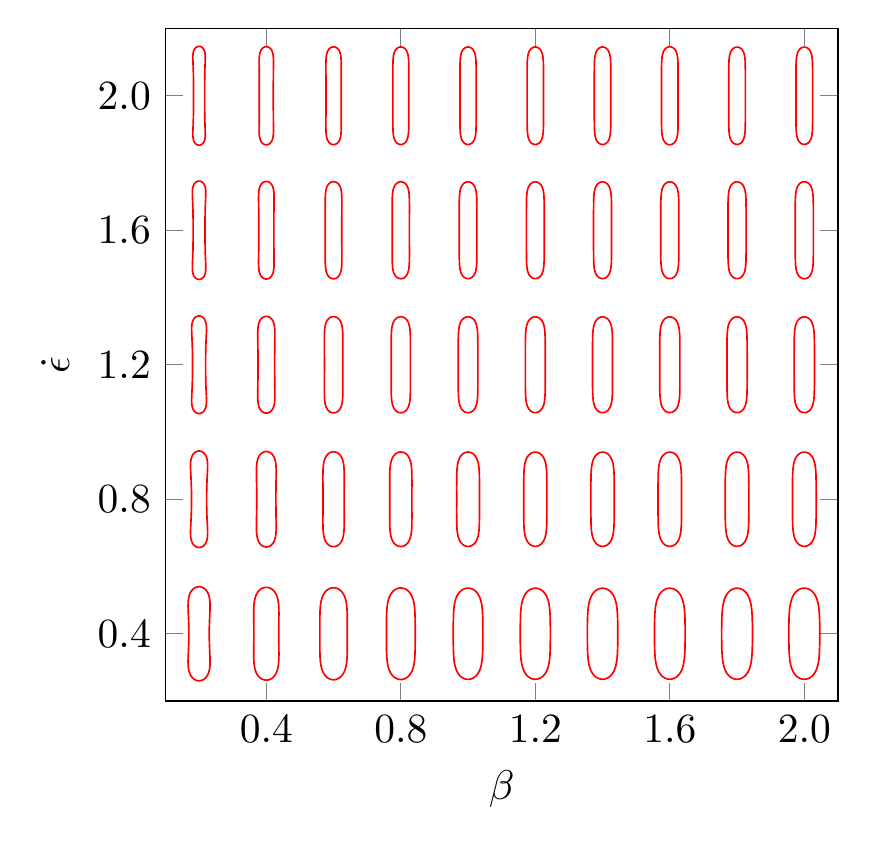
\begin{tikzpicture}[scale=1.5]

  \begin{axis}[
    axis equal image,
    xmin = 1,
    xmax = 21,
    ymin = 2,
    ymax = 22,
    xtick = {4,8,12,16,20},
    xticklabels = {$0.4$,$0.8$,$1.2$,$1.6$,$2.0$},
    xlabel = {$\beta$},
    ytick = {4,8,12,16,20},
    yticklabels = {$0.4$,$0.8$,$1.2$,$1.6$,$2.0$},
    ylabel = {$\dot{\epsilon}$},
  ]

% beta = 0.2,extensional rate = 0.4
\addplot[red] coordinates{
(2.0000e+00,5.3982e+00)
(1.9772e+00,5.3971e+00)
(1.9542e+00,5.3939e+00)
(1.9307e+00,5.3884e+00)
(1.9067e+00,5.3803e+00)
(1.8823e+00,5.3692e+00)
(1.8575e+00,5.3548e+00)
(1.8329e+00,5.3368e+00)
(1.8087e+00,5.3149e+00)
(1.7855e+00,5.2890e+00)
(1.7637e+00,5.2590e+00)
(1.7439e+00,5.2251e+00)
(1.7263e+00,5.1874e+00)
(1.7113e+00,5.1463e+00)
(1.6989e+00,5.1020e+00)
(1.6892e+00,5.0548e+00)
(1.6820e+00,5.0050e+00)
(1.6771e+00,4.9529e+00)
(1.6742e+00,4.8988e+00)
(1.6730e+00,4.8427e+00)
(1.6733e+00,4.7849e+00)
(1.6746e+00,4.7254e+00)
(1.6768e+00,4.6644e+00)
(1.6794e+00,4.6021e+00)
(1.6823e+00,4.5385e+00)
(1.6853e+00,4.4738e+00)
(1.6882e+00,4.4080e+00)
(1.6908e+00,4.3414e+00)
(1.6931e+00,4.2740e+00)
(1.6950e+00,4.2060e+00)
(1.6963e+00,4.1376e+00)
(1.6972e+00,4.0689e+00)
(1.6974e+00,4.0000e+00)
(1.6972e+00,3.9311e+00)
(1.6963e+00,3.8624e+00)
(1.6950e+00,3.7940e+00)
(1.6931e+00,3.7260e+00)
(1.6908e+00,3.6586e+00)
(1.6882e+00,3.5920e+00)
(1.6853e+00,3.5262e+00)
(1.6823e+00,3.4615e+00)
(1.6794e+00,3.3979e+00)
(1.6768e+00,3.3356e+00)
(1.6746e+00,3.2746e+00)
(1.6733e+00,3.2151e+00)
(1.6730e+00,3.1573e+00)
(1.6742e+00,3.1012e+00)
(1.6771e+00,3.0471e+00)
(1.6820e+00,2.9950e+00)
(1.6892e+00,2.9452e+00)
(1.6989e+00,2.8980e+00)
(1.7113e+00,2.8537e+00)
(1.7263e+00,2.8126e+00)
(1.7439e+00,2.7749e+00)
(1.7637e+00,2.7410e+00)
(1.7855e+00,2.7110e+00)
(1.8087e+00,2.6851e+00)
(1.8329e+00,2.6632e+00)
(1.8575e+00,2.6452e+00)
(1.8823e+00,2.6308e+00)
(1.9067e+00,2.6197e+00)
(1.9307e+00,2.6116e+00)
(1.9542e+00,2.6061e+00)
(1.9772e+00,2.6029e+00)
(2.0000e+00,2.6018e+00)
(2.0228e+00,2.6029e+00)
(2.0458e+00,2.6061e+00)
(2.0693e+00,2.6116e+00)
(2.0933e+00,2.6197e+00)
(2.1177e+00,2.6308e+00)
(2.1425e+00,2.6452e+00)
(2.1671e+00,2.6632e+00)
(2.1913e+00,2.6851e+00)
(2.2145e+00,2.7110e+00)
(2.2363e+00,2.7410e+00)
(2.2561e+00,2.7749e+00)
(2.2737e+00,2.8126e+00)
(2.2887e+00,2.8537e+00)
(2.3011e+00,2.8980e+00)
(2.3108e+00,2.9452e+00)
(2.3180e+00,2.9950e+00)
(2.3229e+00,3.0471e+00)
(2.3258e+00,3.1012e+00)
(2.3270e+00,3.1573e+00)
(2.3267e+00,3.2151e+00)
(2.3254e+00,3.2746e+00)
(2.3232e+00,3.3356e+00)
(2.3206e+00,3.3979e+00)
(2.3177e+00,3.4615e+00)
(2.3147e+00,3.5262e+00)
(2.3118e+00,3.5920e+00)
(2.3092e+00,3.6586e+00)
(2.3069e+00,3.7260e+00)
(2.3050e+00,3.7940e+00)
(2.3037e+00,3.8624e+00)
(2.3028e+00,3.9311e+00)
(2.3026e+00,4.0000e+00)
(2.3028e+00,4.0689e+00)
(2.3037e+00,4.1376e+00)
(2.3050e+00,4.2060e+00)
(2.3069e+00,4.2740e+00)
(2.3092e+00,4.3414e+00)
(2.3118e+00,4.4080e+00)
(2.3147e+00,4.4738e+00)
(2.3177e+00,4.5385e+00)
(2.3206e+00,4.6021e+00)
(2.3232e+00,4.6644e+00)
(2.3254e+00,4.7254e+00)
(2.3267e+00,4.7849e+00)
(2.3270e+00,4.8427e+00)
(2.3258e+00,4.8988e+00)
(2.3229e+00,4.9529e+00)
(2.3180e+00,5.0050e+00)
(2.3108e+00,5.0548e+00)
(2.3011e+00,5.1020e+00)
(2.2887e+00,5.1463e+00)
(2.2737e+00,5.1874e+00)
(2.2561e+00,5.2251e+00)
(2.2363e+00,5.2590e+00)
(2.2145e+00,5.2890e+00)
(2.1913e+00,5.3149e+00)
(2.1671e+00,5.3368e+00)
(2.1425e+00,5.3548e+00)
(2.1177e+00,5.3692e+00)
(2.0933e+00,5.3803e+00)
(2.0693e+00,5.3884e+00)
(2.0458e+00,5.3939e+00)
(2.0228e+00,5.3971e+00)
(2.0000e+00,5.3982e+00)
};

% beta = 0.4,extensional rate = 0.4
\addplot[red] coordinates{
(4.0000e+00,5.3793e+00)
(3.9772e+00,5.3784e+00)
(3.9541e+00,5.3755e+00)
(3.9305e+00,5.3705e+00)
(3.9063e+00,5.3631e+00)
(3.8814e+00,5.3530e+00)
(3.8560e+00,5.3398e+00)
(3.8303e+00,5.3232e+00)
(3.8047e+00,5.3028e+00)
(3.7797e+00,5.2786e+00)
(3.7557e+00,5.2504e+00)
(3.7332e+00,5.2182e+00)
(3.7125e+00,5.1822e+00)
(3.6940e+00,5.1424e+00)
(3.6779e+00,5.0994e+00)
(3.6642e+00,5.0532e+00)
(3.6529e+00,5.0042e+00)
(3.6439e+00,4.9526e+00)
(3.6370e+00,4.8988e+00)
(3.6319e+00,4.8430e+00)
(3.6284e+00,4.7852e+00)
(3.6263e+00,4.7258e+00)
(3.6252e+00,4.6648e+00)
(3.6248e+00,4.6024e+00)
(3.6251e+00,4.5388e+00)
(3.6257e+00,4.4740e+00)
(3.6265e+00,4.4081e+00)
(3.6274e+00,4.3415e+00)
(3.6283e+00,4.2741e+00)
(3.6291e+00,4.2061e+00)
(3.6297e+00,4.1376e+00)
(3.6300e+00,4.0689e+00)
(3.6302e+00,4.0000e+00)
(3.6300e+00,3.9311e+00)
(3.6297e+00,3.8624e+00)
(3.6291e+00,3.7939e+00)
(3.6283e+00,3.7259e+00)
(3.6274e+00,3.6585e+00)
(3.6265e+00,3.5919e+00)
(3.6257e+00,3.5260e+00)
(3.6251e+00,3.4612e+00)
(3.6248e+00,3.3976e+00)
(3.6252e+00,3.3352e+00)
(3.6263e+00,3.2742e+00)
(3.6284e+00,3.2148e+00)
(3.6319e+00,3.1570e+00)
(3.6370e+00,3.1012e+00)
(3.6439e+00,3.0474e+00)
(3.6529e+00,2.9958e+00)
(3.6642e+00,2.9468e+00)
(3.6779e+00,2.9006e+00)
(3.6940e+00,2.8576e+00)
(3.7125e+00,2.8178e+00)
(3.7332e+00,2.7818e+00)
(3.7557e+00,2.7496e+00)
(3.7797e+00,2.7214e+00)
(3.8047e+00,2.6972e+00)
(3.8303e+00,2.6768e+00)
(3.8560e+00,2.6602e+00)
(3.8814e+00,2.6470e+00)
(3.9063e+00,2.6369e+00)
(3.9305e+00,2.6295e+00)
(3.9541e+00,2.6245e+00)
(3.9772e+00,2.6216e+00)
(4.0000e+00,2.6207e+00)
(4.0228e+00,2.6216e+00)
(4.0459e+00,2.6245e+00)
(4.0695e+00,2.6295e+00)
(4.0937e+00,2.6369e+00)
(4.1186e+00,2.6470e+00)
(4.1440e+00,2.6602e+00)
(4.1697e+00,2.6768e+00)
(4.1953e+00,2.6972e+00)
(4.2203e+00,2.7214e+00)
(4.2443e+00,2.7496e+00)
(4.2668e+00,2.7818e+00)
(4.2875e+00,2.8178e+00)
(4.3060e+00,2.8576e+00)
(4.3221e+00,2.9006e+00)
(4.3358e+00,2.9468e+00)
(4.3471e+00,2.9958e+00)
(4.3561e+00,3.0474e+00)
(4.3630e+00,3.1012e+00)
(4.3681e+00,3.1570e+00)
(4.3716e+00,3.2148e+00)
(4.3737e+00,3.2742e+00)
(4.3748e+00,3.3352e+00)
(4.3752e+00,3.3976e+00)
(4.3749e+00,3.4612e+00)
(4.3743e+00,3.5260e+00)
(4.3735e+00,3.5919e+00)
(4.3726e+00,3.6585e+00)
(4.3717e+00,3.7259e+00)
(4.3709e+00,3.7939e+00)
(4.3703e+00,3.8624e+00)
(4.3700e+00,3.9311e+00)
(4.3698e+00,4.0000e+00)
(4.3700e+00,4.0689e+00)
(4.3703e+00,4.1376e+00)
(4.3709e+00,4.2061e+00)
(4.3717e+00,4.2741e+00)
(4.3726e+00,4.3415e+00)
(4.3735e+00,4.4081e+00)
(4.3743e+00,4.4740e+00)
(4.3749e+00,4.5388e+00)
(4.3752e+00,4.6024e+00)
(4.3748e+00,4.6648e+00)
(4.3737e+00,4.7258e+00)
(4.3716e+00,4.7852e+00)
(4.3681e+00,4.8430e+00)
(4.3630e+00,4.8988e+00)
(4.3561e+00,4.9526e+00)
(4.3471e+00,5.0042e+00)
(4.3358e+00,5.0532e+00)
(4.3221e+00,5.0994e+00)
(4.3060e+00,5.1424e+00)
(4.2875e+00,5.1822e+00)
(4.2668e+00,5.2182e+00)
(4.2443e+00,5.2504e+00)
(4.2203e+00,5.2786e+00)
(4.1953e+00,5.3028e+00)
(4.1697e+00,5.3232e+00)
(4.1440e+00,5.3398e+00)
(4.1186e+00,5.3530e+00)
(4.0937e+00,5.3631e+00)
(4.0695e+00,5.3705e+00)
(4.0459e+00,5.3755e+00)
(4.0228e+00,5.3784e+00)
(4.0000e+00,5.3793e+00)
};

% beta = 0.6,extensional rate = 0.4
\addplot[red] coordinates{
(6.0000e+00,5.3676e+00)
(5.9772e+00,5.3667e+00)
(5.9541e+00,5.3639e+00)
(5.9305e+00,5.3592e+00)
(5.9061e+00,5.3522e+00)
(5.8809e+00,5.3425e+00)
(5.8551e+00,5.3300e+00)
(5.8290e+00,5.3141e+00)
(5.8027e+00,5.2946e+00)
(5.7768e+00,5.2713e+00)
(5.7517e+00,5.2441e+00)
(5.7278e+00,5.2129e+00)
(5.7055e+00,5.1778e+00)
(5.6852e+00,5.1390e+00)
(5.6670e+00,5.0967e+00)
(5.6511e+00,5.0512e+00)
(5.6376e+00,5.0028e+00)
(5.6263e+00,4.9517e+00)
(5.6171e+00,4.8982e+00)
(5.6099e+00,4.8426e+00)
(5.6043e+00,4.7850e+00)
(5.6001e+00,4.7257e+00)
(5.5971e+00,4.6648e+00)
(5.5951e+00,4.6024e+00)
(5.5938e+00,4.5388e+00)
(5.5931e+00,4.4740e+00)
(5.5928e+00,4.4082e+00)
(5.5927e+00,4.3415e+00)
(5.5928e+00,4.2741e+00)
(5.5929e+00,4.2061e+00)
(5.5930e+00,4.1376e+00)
(5.5931e+00,4.0689e+00)
(5.5932e+00,4.0000e+00)
(5.5931e+00,3.9311e+00)
(5.5930e+00,3.8624e+00)
(5.5929e+00,3.7939e+00)
(5.5928e+00,3.7259e+00)
(5.5927e+00,3.6585e+00)
(5.5928e+00,3.5918e+00)
(5.5931e+00,3.5260e+00)
(5.5938e+00,3.4612e+00)
(5.5951e+00,3.3976e+00)
(5.5971e+00,3.3352e+00)
(5.6001e+00,3.2743e+00)
(5.6043e+00,3.2150e+00)
(5.6099e+00,3.1574e+00)
(5.6171e+00,3.1018e+00)
(5.6263e+00,3.0483e+00)
(5.6376e+00,2.9972e+00)
(5.6511e+00,2.9488e+00)
(5.6670e+00,2.9033e+00)
(5.6852e+00,2.8610e+00)
(5.7055e+00,2.8222e+00)
(5.7278e+00,2.7871e+00)
(5.7517e+00,2.7559e+00)
(5.7768e+00,2.7287e+00)
(5.8027e+00,2.7054e+00)
(5.8290e+00,2.6859e+00)
(5.8551e+00,2.6700e+00)
(5.8809e+00,2.6575e+00)
(5.9061e+00,2.6478e+00)
(5.9305e+00,2.6408e+00)
(5.9541e+00,2.6361e+00)
(5.9772e+00,2.6333e+00)
(6.0000e+00,2.6324e+00)
(6.0228e+00,2.6333e+00)
(6.0459e+00,2.6361e+00)
(6.0695e+00,2.6408e+00)
(6.0939e+00,2.6478e+00)
(6.1191e+00,2.6575e+00)
(6.1449e+00,2.6700e+00)
(6.1710e+00,2.6859e+00)
(6.1973e+00,2.7054e+00)
(6.2232e+00,2.7287e+00)
(6.2483e+00,2.7559e+00)
(6.2722e+00,2.7871e+00)
(6.2945e+00,2.8222e+00)
(6.3148e+00,2.8610e+00)
(6.3330e+00,2.9033e+00)
(6.3489e+00,2.9488e+00)
(6.3624e+00,2.9972e+00)
(6.3737e+00,3.0483e+00)
(6.3829e+00,3.1018e+00)
(6.3901e+00,3.1574e+00)
(6.3957e+00,3.2150e+00)
(6.3999e+00,3.2743e+00)
(6.4029e+00,3.3352e+00)
(6.4049e+00,3.3976e+00)
(6.4062e+00,3.4612e+00)
(6.4069e+00,3.5260e+00)
(6.4072e+00,3.5918e+00)
(6.4073e+00,3.6585e+00)
(6.4072e+00,3.7259e+00)
(6.4071e+00,3.7939e+00)
(6.4070e+00,3.8624e+00)
(6.4069e+00,3.9311e+00)
(6.4068e+00,4.0000e+00)
(6.4069e+00,4.0689e+00)
(6.4070e+00,4.1376e+00)
(6.4071e+00,4.2061e+00)
(6.4072e+00,4.2741e+00)
(6.4073e+00,4.3415e+00)
(6.4072e+00,4.4082e+00)
(6.4069e+00,4.4740e+00)
(6.4062e+00,4.5388e+00)
(6.4049e+00,4.6024e+00)
(6.4029e+00,4.6648e+00)
(6.3999e+00,4.7257e+00)
(6.3957e+00,4.7850e+00)
(6.3901e+00,4.8426e+00)
(6.3829e+00,4.8982e+00)
(6.3737e+00,4.9517e+00)
(6.3624e+00,5.0028e+00)
(6.3489e+00,5.0512e+00)
(6.3330e+00,5.0967e+00)
(6.3148e+00,5.1390e+00)
(6.2945e+00,5.1778e+00)
(6.2722e+00,5.2129e+00)
(6.2483e+00,5.2441e+00)
(6.2232e+00,5.2713e+00)
(6.1973e+00,5.2946e+00)
(6.1710e+00,5.3141e+00)
(6.1449e+00,5.3300e+00)
(6.1191e+00,5.3425e+00)
(6.0939e+00,5.3522e+00)
(6.0695e+00,5.3592e+00)
(6.0459e+00,5.3639e+00)
(6.0228e+00,5.3667e+00)
(6.0000e+00,5.3676e+00)
};

% beta = 0.8,extensional rate = 0.4
\addplot[red] coordinates{
(8.0000e+00,5.3607e+00)
(7.9772e+00,5.3599e+00)
(7.9541e+00,5.3572e+00)
(7.9304e+00,5.3526e+00)
(7.9059e+00,5.3458e+00)
(7.8807e+00,5.3364e+00)
(7.8547e+00,5.3241e+00)
(7.8283e+00,5.3086e+00)
(7.8016e+00,5.2896e+00)
(7.7753e+00,5.2668e+00)
(7.7496e+00,5.2401e+00)
(7.7249e+00,5.2095e+00)
(7.7018e+00,5.1749e+00)
(7.6805e+00,5.1367e+00)
(7.6612e+00,5.0949e+00)
(7.6442e+00,5.0498e+00)
(7.6294e+00,5.0017e+00)
(7.6169e+00,4.9509e+00)
(7.6064e+00,4.8977e+00)
(7.5979e+00,4.8422e+00)
(7.5911e+00,4.7848e+00)
(7.5858e+00,4.7256e+00)
(7.5817e+00,4.6647e+00)
(7.5787e+00,4.6024e+00)
(7.5765e+00,4.5388e+00)
(7.5750e+00,4.4740e+00)
(7.5739e+00,4.4082e+00)
(7.5733e+00,4.3415e+00)
(7.5729e+00,4.2741e+00)
(7.5726e+00,4.2061e+00)
(7.5725e+00,4.1376e+00)
(7.5724e+00,4.0689e+00)
(7.5724e+00,4.0000e+00)
(7.5724e+00,3.9311e+00)
(7.5725e+00,3.8624e+00)
(7.5726e+00,3.7939e+00)
(7.5729e+00,3.7259e+00)
(7.5733e+00,3.6585e+00)
(7.5739e+00,3.5918e+00)
(7.5750e+00,3.5260e+00)
(7.5765e+00,3.4612e+00)
(7.5787e+00,3.3976e+00)
(7.5817e+00,3.3353e+00)
(7.5858e+00,3.2744e+00)
(7.5911e+00,3.2152e+00)
(7.5979e+00,3.1578e+00)
(7.6064e+00,3.1023e+00)
(7.6169e+00,3.0491e+00)
(7.6294e+00,2.9983e+00)
(7.6442e+00,2.9502e+00)
(7.6612e+00,2.9051e+00)
(7.6805e+00,2.8633e+00)
(7.7018e+00,2.8251e+00)
(7.7249e+00,2.7905e+00)
(7.7496e+00,2.7599e+00)
(7.7753e+00,2.7332e+00)
(7.8016e+00,2.7104e+00)
(7.8283e+00,2.6914e+00)
(7.8547e+00,2.6759e+00)
(7.8807e+00,2.6636e+00)
(7.9059e+00,2.6542e+00)
(7.9304e+00,2.6474e+00)
(7.9541e+00,2.6428e+00)
(7.9772e+00,2.6401e+00)
(8.0000e+00,2.6393e+00)
(8.0228e+00,2.6401e+00)
(8.0459e+00,2.6428e+00)
(8.0696e+00,2.6474e+00)
(8.0941e+00,2.6542e+00)
(8.1193e+00,2.6636e+00)
(8.1453e+00,2.6759e+00)
(8.1717e+00,2.6914e+00)
(8.1984e+00,2.7104e+00)
(8.2247e+00,2.7332e+00)
(8.2504e+00,2.7599e+00)
(8.2751e+00,2.7905e+00)
(8.2982e+00,2.8251e+00)
(8.3195e+00,2.8633e+00)
(8.3388e+00,2.9051e+00)
(8.3558e+00,2.9502e+00)
(8.3706e+00,2.9983e+00)
(8.3831e+00,3.0491e+00)
(8.3936e+00,3.1023e+00)
(8.4021e+00,3.1578e+00)
(8.4089e+00,3.2152e+00)
(8.4142e+00,3.2744e+00)
(8.4183e+00,3.3353e+00)
(8.4213e+00,3.3976e+00)
(8.4235e+00,3.4612e+00)
(8.4250e+00,3.5260e+00)
(8.4261e+00,3.5918e+00)
(8.4267e+00,3.6585e+00)
(8.4271e+00,3.7259e+00)
(8.4274e+00,3.7939e+00)
(8.4275e+00,3.8624e+00)
(8.4276e+00,3.9311e+00)
(8.4276e+00,4.0000e+00)
(8.4276e+00,4.0689e+00)
(8.4275e+00,4.1376e+00)
(8.4274e+00,4.2061e+00)
(8.4271e+00,4.2741e+00)
(8.4267e+00,4.3415e+00)
(8.4261e+00,4.4082e+00)
(8.4250e+00,4.4740e+00)
(8.4235e+00,4.5388e+00)
(8.4213e+00,4.6024e+00)
(8.4183e+00,4.6647e+00)
(8.4142e+00,4.7256e+00)
(8.4089e+00,4.7848e+00)
(8.4021e+00,4.8422e+00)
(8.3936e+00,4.8977e+00)
(8.3831e+00,4.9509e+00)
(8.3706e+00,5.0017e+00)
(8.3558e+00,5.0498e+00)
(8.3388e+00,5.0949e+00)
(8.3195e+00,5.1367e+00)
(8.2982e+00,5.1749e+00)
(8.2751e+00,5.2095e+00)
(8.2504e+00,5.2401e+00)
(8.2247e+00,5.2668e+00)
(8.1984e+00,5.2896e+00)
(8.1717e+00,5.3086e+00)
(8.1453e+00,5.3241e+00)
(8.1193e+00,5.3364e+00)
(8.0941e+00,5.3458e+00)
(8.0696e+00,5.3526e+00)
(8.0459e+00,5.3572e+00)
(8.0228e+00,5.3599e+00)
(8.0000e+00,5.3607e+00)
};

% beta = 1,extensional rate = 0.4
\addplot[red] coordinates{
(1.0000e+01,5.3567e+00)
(9.9772e+00,5.3559e+00)
(9.9541e+00,5.3533e+00)
(9.9304e+00,5.3488e+00)
(9.9059e+00,5.3421e+00)
(9.8805e+00,5.3328e+00)
(9.8544e+00,5.3207e+00)
(9.8278e+00,5.3054e+00)
(9.8010e+00,5.2866e+00)
(9.7743e+00,5.2641e+00)
(9.7483e+00,5.2377e+00)
(9.7232e+00,5.2074e+00)
(9.6996e+00,5.1731e+00)
(9.6777e+00,5.1352e+00)
(9.6579e+00,5.0937e+00)
(9.6402e+00,5.0489e+00)
(9.6247e+00,5.0010e+00)
(9.6114e+00,4.9504e+00)
(9.6002e+00,4.8973e+00)
(9.5909e+00,4.8420e+00)
(9.5834e+00,4.7846e+00)
(9.5774e+00,4.7254e+00)
(9.5727e+00,4.6646e+00)
(9.5691e+00,4.6023e+00)
(9.5663e+00,4.5387e+00)
(9.5643e+00,4.4740e+00)
(9.5629e+00,4.4082e+00)
(9.5618e+00,4.3415e+00)
(9.5611e+00,4.2741e+00)
(9.5607e+00,4.2061e+00)
(9.5604e+00,4.1376e+00)
(9.5602e+00,4.0689e+00)
(9.5602e+00,4.0000e+00)
(9.5602e+00,3.9311e+00)
(9.5604e+00,3.8624e+00)
(9.5607e+00,3.7939e+00)
(9.5611e+00,3.7259e+00)
(9.5618e+00,3.6585e+00)
(9.5629e+00,3.5918e+00)
(9.5643e+00,3.5260e+00)
(9.5663e+00,3.4613e+00)
(9.5691e+00,3.3977e+00)
(9.5727e+00,3.3354e+00)
(9.5774e+00,3.2746e+00)
(9.5834e+00,3.2154e+00)
(9.5909e+00,3.1580e+00)
(9.6002e+00,3.1027e+00)
(9.6114e+00,3.0496e+00)
(9.6247e+00,2.9990e+00)
(9.6402e+00,2.9511e+00)
(9.6579e+00,2.9063e+00)
(9.6777e+00,2.8648e+00)
(9.6996e+00,2.8269e+00)
(9.7232e+00,2.7926e+00)
(9.7483e+00,2.7623e+00)
(9.7743e+00,2.7359e+00)
(9.8010e+00,2.7134e+00)
(9.8278e+00,2.6946e+00)
(9.8544e+00,2.6793e+00)
(9.8805e+00,2.6672e+00)
(9.9059e+00,2.6579e+00)
(9.9304e+00,2.6512e+00)
(9.9541e+00,2.6467e+00)
(9.9772e+00,2.6441e+00)
(1.0000e+01,2.6433e+00)
(1.0023e+01,2.6441e+00)
(1.0046e+01,2.6467e+00)
(1.0070e+01,2.6512e+00)
(1.0094e+01,2.6579e+00)
(1.0119e+01,2.6672e+00)
(1.0146e+01,2.6793e+00)
(1.0172e+01,2.6946e+00)
(1.0199e+01,2.7134e+00)
(1.0226e+01,2.7359e+00)
(1.0252e+01,2.7623e+00)
(1.0277e+01,2.7926e+00)
(1.0300e+01,2.8269e+00)
(1.0322e+01,2.8648e+00)
(1.0342e+01,2.9063e+00)
(1.0360e+01,2.9511e+00)
(1.0375e+01,2.9990e+00)
(1.0389e+01,3.0496e+00)
(1.0400e+01,3.1027e+00)
(1.0409e+01,3.1580e+00)
(1.0417e+01,3.2154e+00)
(1.0423e+01,3.2746e+00)
(1.0427e+01,3.3354e+00)
(1.0431e+01,3.3977e+00)
(1.0434e+01,3.4613e+00)
(1.0436e+01,3.5260e+00)
(1.0437e+01,3.5918e+00)
(1.0438e+01,3.6585e+00)
(1.0439e+01,3.7259e+00)
(1.0439e+01,3.7939e+00)
(1.0440e+01,3.8624e+00)
(1.0440e+01,3.9311e+00)
(1.0440e+01,4.0000e+00)
(1.0440e+01,4.0689e+00)
(1.0440e+01,4.1376e+00)
(1.0439e+01,4.2061e+00)
(1.0439e+01,4.2741e+00)
(1.0438e+01,4.3415e+00)
(1.0437e+01,4.4082e+00)
(1.0436e+01,4.4740e+00)
(1.0434e+01,4.5387e+00)
(1.0431e+01,4.6023e+00)
(1.0427e+01,4.6646e+00)
(1.0423e+01,4.7254e+00)
(1.0417e+01,4.7846e+00)
(1.0409e+01,4.8420e+00)
(1.0400e+01,4.8973e+00)
(1.0389e+01,4.9504e+00)
(1.0375e+01,5.0010e+00)
(1.0360e+01,5.0489e+00)
(1.0342e+01,5.0937e+00)
(1.0322e+01,5.1352e+00)
(1.0300e+01,5.1731e+00)
(1.0277e+01,5.2074e+00)
(1.0252e+01,5.2377e+00)
(1.0226e+01,5.2641e+00)
(1.0199e+01,5.2866e+00)
(1.0172e+01,5.3054e+00)
(1.0146e+01,5.3207e+00)
(1.0119e+01,5.3328e+00)
(1.0094e+01,5.3421e+00)
(1.0070e+01,5.3488e+00)
(1.0046e+01,5.3533e+00)
(1.0023e+01,5.3559e+00)
(1.0000e+01,5.3567e+00)
};

% beta = 1.2,extensional rate = 0.4
\addplot[red] coordinates{
(1.2000e+01,5.3545e+00)
(1.1977e+01,5.3536e+00)
(1.1954e+01,5.3511e+00)
(1.1930e+01,5.3466e+00)
(1.1906e+01,5.3399e+00)
(1.1880e+01,5.3308e+00)
(1.1854e+01,5.3188e+00)
(1.1827e+01,5.3036e+00)
(1.1800e+01,5.2849e+00)
(1.1774e+01,5.2625e+00)
(1.1747e+01,5.2362e+00)
(1.1722e+01,5.2061e+00)
(1.1698e+01,5.1720e+00)
(1.1676e+01,5.1343e+00)
(1.1656e+01,5.0929e+00)
(1.1638e+01,5.0483e+00)
(1.1622e+01,5.0006e+00)
(1.1608e+01,4.9501e+00)
(1.1596e+01,4.8971e+00)
(1.1587e+01,4.8418e+00)
(1.1579e+01,4.7845e+00)
(1.1572e+01,4.7254e+00)
(1.1567e+01,4.6646e+00)
(1.1563e+01,4.6023e+00)
(1.1560e+01,4.5387e+00)
(1.1558e+01,4.4739e+00)
(1.1556e+01,4.4081e+00)
(1.1555e+01,4.3415e+00)
(1.1554e+01,4.2741e+00)
(1.1553e+01,4.2061e+00)
(1.1553e+01,4.1376e+00)
(1.1553e+01,4.0689e+00)
(1.1552e+01,4.0000e+00)
(1.1553e+01,3.9311e+00)
(1.1553e+01,3.8624e+00)
(1.1553e+01,3.7939e+00)
(1.1554e+01,3.7259e+00)
(1.1555e+01,3.6585e+00)
(1.1556e+01,3.5919e+00)
(1.1558e+01,3.5261e+00)
(1.1560e+01,3.4613e+00)
(1.1563e+01,3.3977e+00)
(1.1567e+01,3.3354e+00)
(1.1572e+01,3.2746e+00)
(1.1579e+01,3.2155e+00)
(1.1587e+01,3.1582e+00)
(1.1596e+01,3.1029e+00)
(1.1608e+01,3.0499e+00)
(1.1622e+01,2.9994e+00)
(1.1638e+01,2.9517e+00)
(1.1656e+01,2.9071e+00)
(1.1676e+01,2.8657e+00)
(1.1698e+01,2.8280e+00)
(1.1722e+01,2.7939e+00)
(1.1747e+01,2.7638e+00)
(1.1774e+01,2.7375e+00)
(1.1800e+01,2.7151e+00)
(1.1827e+01,2.6964e+00)
(1.1854e+01,2.6812e+00)
(1.1880e+01,2.6692e+00)
(1.1906e+01,2.6601e+00)
(1.1930e+01,2.6534e+00)
(1.1954e+01,2.6489e+00)
(1.1977e+01,2.6464e+00)
(1.2000e+01,2.6455e+00)
(1.2023e+01,2.6464e+00)
(1.2046e+01,2.6489e+00)
(1.2070e+01,2.6534e+00)
(1.2094e+01,2.6601e+00)
(1.2120e+01,2.6692e+00)
(1.2146e+01,2.6812e+00)
(1.2173e+01,2.6964e+00)
(1.2200e+01,2.7151e+00)
(1.2226e+01,2.7375e+00)
(1.2253e+01,2.7638e+00)
(1.2278e+01,2.7939e+00)
(1.2302e+01,2.8280e+00)
(1.2324e+01,2.8657e+00)
(1.2344e+01,2.9071e+00)
(1.2362e+01,2.9517e+00)
(1.2378e+01,2.9994e+00)
(1.2392e+01,3.0499e+00)
(1.2404e+01,3.1029e+00)
(1.2413e+01,3.1582e+00)
(1.2421e+01,3.2155e+00)
(1.2428e+01,3.2746e+00)
(1.2433e+01,3.3354e+00)
(1.2437e+01,3.3977e+00)
(1.2440e+01,3.4613e+00)
(1.2442e+01,3.5261e+00)
(1.2444e+01,3.5919e+00)
(1.2445e+01,3.6585e+00)
(1.2446e+01,3.7259e+00)
(1.2447e+01,3.7939e+00)
(1.2447e+01,3.8624e+00)
(1.2447e+01,3.9311e+00)
(1.2448e+01,4.0000e+00)
(1.2447e+01,4.0689e+00)
(1.2447e+01,4.1376e+00)
(1.2447e+01,4.2061e+00)
(1.2446e+01,4.2741e+00)
(1.2445e+01,4.3415e+00)
(1.2444e+01,4.4081e+00)
(1.2442e+01,4.4739e+00)
(1.2440e+01,4.5387e+00)
(1.2437e+01,4.6023e+00)
(1.2433e+01,4.6646e+00)
(1.2428e+01,4.7254e+00)
(1.2421e+01,4.7845e+00)
(1.2413e+01,4.8418e+00)
(1.2404e+01,4.8971e+00)
(1.2392e+01,4.9501e+00)
(1.2378e+01,5.0006e+00)
(1.2362e+01,5.0483e+00)
(1.2344e+01,5.0929e+00)
(1.2324e+01,5.1343e+00)
(1.2302e+01,5.1720e+00)
(1.2278e+01,5.2061e+00)
(1.2253e+01,5.2362e+00)
(1.2226e+01,5.2625e+00)
(1.2200e+01,5.2849e+00)
(1.2173e+01,5.3036e+00)
(1.2146e+01,5.3188e+00)
(1.2120e+01,5.3308e+00)
(1.2094e+01,5.3399e+00)
(1.2070e+01,5.3466e+00)
(1.2046e+01,5.3511e+00)
(1.2023e+01,5.3536e+00)
(1.2000e+01,5.3545e+00)
};

% beta = 1.4,extensional rate = 0.4
\addplot[red] coordinates{
(1.4000e+01,5.3533e+00)
(1.3977e+01,5.3525e+00)
(1.3954e+01,5.3500e+00)
(1.3930e+01,5.3455e+00)
(1.3906e+01,5.3389e+00)
(1.3880e+01,5.3298e+00)
(1.3854e+01,5.3178e+00)
(1.3827e+01,5.3027e+00)
(1.3800e+01,5.2840e+00)
(1.3773e+01,5.2616e+00)
(1.3747e+01,5.2354e+00)
(1.3721e+01,5.2053e+00)
(1.3697e+01,5.1714e+00)
(1.3675e+01,5.1337e+00)
(1.3654e+01,5.0925e+00)
(1.3636e+01,5.0479e+00)
(1.3620e+01,5.0003e+00)
(1.3606e+01,4.9499e+00)
(1.3594e+01,4.8969e+00)
(1.3584e+01,4.8417e+00)
(1.3575e+01,4.7845e+00)
(1.3569e+01,4.7253e+00)
(1.3563e+01,4.6646e+00)
(1.3559e+01,4.6023e+00)
(1.3556e+01,4.5387e+00)
(1.3553e+01,4.4739e+00)
(1.3551e+01,4.4081e+00)
(1.3550e+01,4.3415e+00)
(1.3549e+01,4.2741e+00)
(1.3548e+01,4.2061e+00)
(1.3548e+01,4.1376e+00)
(1.3548e+01,4.0689e+00)
(1.3547e+01,4.0000e+00)
(1.3548e+01,3.9311e+00)
(1.3548e+01,3.8624e+00)
(1.3548e+01,3.7939e+00)
(1.3549e+01,3.7259e+00)
(1.3550e+01,3.6585e+00)
(1.3551e+01,3.5919e+00)
(1.3553e+01,3.5261e+00)
(1.3556e+01,3.4613e+00)
(1.3559e+01,3.3977e+00)
(1.3563e+01,3.3354e+00)
(1.3569e+01,3.2747e+00)
(1.3575e+01,3.2155e+00)
(1.3584e+01,3.1583e+00)
(1.3594e+01,3.1031e+00)
(1.3606e+01,3.0501e+00)
(1.3620e+01,2.9997e+00)
(1.3636e+01,2.9521e+00)
(1.3654e+01,2.9075e+00)
(1.3675e+01,2.8663e+00)
(1.3697e+01,2.8286e+00)
(1.3721e+01,2.7947e+00)
(1.3747e+01,2.7646e+00)
(1.3773e+01,2.7384e+00)
(1.3800e+01,2.7160e+00)
(1.3827e+01,2.6973e+00)
(1.3854e+01,2.6822e+00)
(1.3880e+01,2.6702e+00)
(1.3906e+01,2.6611e+00)
(1.3930e+01,2.6545e+00)
(1.3954e+01,2.6500e+00)
(1.3977e+01,2.6475e+00)
(1.4000e+01,2.6467e+00)
(1.4023e+01,2.6475e+00)
(1.4046e+01,2.6500e+00)
(1.4070e+01,2.6545e+00)
(1.4094e+01,2.6611e+00)
(1.4120e+01,2.6702e+00)
(1.4146e+01,2.6822e+00)
(1.4173e+01,2.6973e+00)
(1.4200e+01,2.7160e+00)
(1.4227e+01,2.7384e+00)
(1.4253e+01,2.7646e+00)
(1.4279e+01,2.7947e+00)
(1.4303e+01,2.8286e+00)
(1.4325e+01,2.8663e+00)
(1.4346e+01,2.9075e+00)
(1.4364e+01,2.9521e+00)
(1.4380e+01,2.9997e+00)
(1.4394e+01,3.0501e+00)
(1.4406e+01,3.1031e+00)
(1.4416e+01,3.1583e+00)
(1.4425e+01,3.2155e+00)
(1.4431e+01,3.2747e+00)
(1.4437e+01,3.3354e+00)
(1.4441e+01,3.3977e+00)
(1.4444e+01,3.4613e+00)
(1.4447e+01,3.5261e+00)
(1.4449e+01,3.5919e+00)
(1.4450e+01,3.6585e+00)
(1.4451e+01,3.7259e+00)
(1.4452e+01,3.7939e+00)
(1.4452e+01,3.8624e+00)
(1.4452e+01,3.9311e+00)
(1.4453e+01,4.0000e+00)
(1.4452e+01,4.0689e+00)
(1.4452e+01,4.1376e+00)
(1.4452e+01,4.2061e+00)
(1.4451e+01,4.2741e+00)
(1.4450e+01,4.3415e+00)
(1.4449e+01,4.4081e+00)
(1.4447e+01,4.4739e+00)
(1.4444e+01,4.5387e+00)
(1.4441e+01,4.6023e+00)
(1.4437e+01,4.6646e+00)
(1.4431e+01,4.7253e+00)
(1.4425e+01,4.7845e+00)
(1.4416e+01,4.8417e+00)
(1.4406e+01,4.8969e+00)
(1.4394e+01,4.9499e+00)
(1.4380e+01,5.0003e+00)
(1.4364e+01,5.0479e+00)
(1.4346e+01,5.0925e+00)
(1.4325e+01,5.1337e+00)
(1.4303e+01,5.1714e+00)
(1.4279e+01,5.2053e+00)
(1.4253e+01,5.2354e+00)
(1.4227e+01,5.2616e+00)
(1.4200e+01,5.2840e+00)
(1.4173e+01,5.3027e+00)
(1.4146e+01,5.3178e+00)
(1.4120e+01,5.3298e+00)
(1.4094e+01,5.3389e+00)
(1.4070e+01,5.3455e+00)
(1.4046e+01,5.3500e+00)
(1.4023e+01,5.3525e+00)
(1.4000e+01,5.3533e+00)
};

% beta = 1.6,extensional rate = 0.4
\addplot[red] coordinates{
(1.6000e+01,5.3531e+00)
(1.5977e+01,5.3523e+00)
(1.5954e+01,5.3497e+00)
(1.5930e+01,5.3453e+00)
(1.5906e+01,5.3387e+00)
(1.5880e+01,5.3296e+00)
(1.5854e+01,5.3177e+00)
(1.5827e+01,5.3025e+00)
(1.5799e+01,5.2838e+00)
(1.5772e+01,5.2614e+00)
(1.5746e+01,5.2351e+00)
(1.5720e+01,5.2050e+00)
(1.5696e+01,5.1711e+00)
(1.5674e+01,5.1334e+00)
(1.5653e+01,5.0922e+00)
(1.5635e+01,5.0477e+00)
(1.5618e+01,5.0002e+00)
(1.5604e+01,4.9498e+00)
(1.5592e+01,4.8969e+00)
(1.5582e+01,4.8417e+00)
(1.5573e+01,4.7845e+00)
(1.5566e+01,4.7253e+00)
(1.5561e+01,4.6646e+00)
(1.5556e+01,4.6023e+00)
(1.5553e+01,4.5387e+00)
(1.5550e+01,4.4739e+00)
(1.5548e+01,4.4082e+00)
(1.5547e+01,4.3415e+00)
(1.5546e+01,4.2741e+00)
(1.5545e+01,4.2061e+00)
(1.5544e+01,4.1376e+00)
(1.5544e+01,4.0689e+00)
(1.5544e+01,4.0000e+00)
(1.5544e+01,3.9311e+00)
(1.5544e+01,3.8624e+00)
(1.5545e+01,3.7939e+00)
(1.5546e+01,3.7259e+00)
(1.5547e+01,3.6585e+00)
(1.5548e+01,3.5918e+00)
(1.5550e+01,3.5261e+00)
(1.5553e+01,3.4613e+00)
(1.5556e+01,3.3977e+00)
(1.5561e+01,3.3354e+00)
(1.5566e+01,3.2747e+00)
(1.5573e+01,3.2155e+00)
(1.5582e+01,3.1583e+00)
(1.5592e+01,3.1031e+00)
(1.5604e+01,3.0502e+00)
(1.5618e+01,2.9998e+00)
(1.5635e+01,2.9523e+00)
(1.5653e+01,2.9078e+00)
(1.5674e+01,2.8666e+00)
(1.5696e+01,2.8289e+00)
(1.5720e+01,2.7950e+00)
(1.5746e+01,2.7649e+00)
(1.5772e+01,2.7386e+00)
(1.5799e+01,2.7162e+00)
(1.5827e+01,2.6975e+00)
(1.5854e+01,2.6823e+00)
(1.5880e+01,2.6704e+00)
(1.5906e+01,2.6613e+00)
(1.5930e+01,2.6547e+00)
(1.5954e+01,2.6503e+00)
(1.5977e+01,2.6477e+00)
(1.6000e+01,2.6469e+00)
(1.6023e+01,2.6477e+00)
(1.6046e+01,2.6503e+00)
(1.6070e+01,2.6547e+00)
(1.6094e+01,2.6613e+00)
(1.6120e+01,2.6704e+00)
(1.6146e+01,2.6823e+00)
(1.6173e+01,2.6975e+00)
(1.6201e+01,2.7162e+00)
(1.6228e+01,2.7386e+00)
(1.6254e+01,2.7649e+00)
(1.6280e+01,2.7950e+00)
(1.6304e+01,2.8289e+00)
(1.6326e+01,2.8666e+00)
(1.6347e+01,2.9078e+00)
(1.6365e+01,2.9523e+00)
(1.6382e+01,2.9998e+00)
(1.6396e+01,3.0502e+00)
(1.6408e+01,3.1031e+00)
(1.6418e+01,3.1583e+00)
(1.6427e+01,3.2155e+00)
(1.6434e+01,3.2747e+00)
(1.6439e+01,3.3354e+00)
(1.6444e+01,3.3977e+00)
(1.6447e+01,3.4613e+00)
(1.6450e+01,3.5261e+00)
(1.6452e+01,3.5918e+00)
(1.6453e+01,3.6585e+00)
(1.6454e+01,3.7259e+00)
(1.6455e+01,3.7939e+00)
(1.6456e+01,3.8624e+00)
(1.6456e+01,3.9311e+00)
(1.6456e+01,4.0000e+00)
(1.6456e+01,4.0689e+00)
(1.6456e+01,4.1376e+00)
(1.6455e+01,4.2061e+00)
(1.6454e+01,4.2741e+00)
(1.6453e+01,4.3415e+00)
(1.6452e+01,4.4082e+00)
(1.6450e+01,4.4739e+00)
(1.6447e+01,4.5387e+00)
(1.6444e+01,4.6023e+00)
(1.6439e+01,4.6646e+00)
(1.6434e+01,4.7253e+00)
(1.6427e+01,4.7845e+00)
(1.6418e+01,4.8417e+00)
(1.6408e+01,4.8969e+00)
(1.6396e+01,4.9498e+00)
(1.6382e+01,5.0002e+00)
(1.6365e+01,5.0477e+00)
(1.6347e+01,5.0922e+00)
(1.6326e+01,5.1334e+00)
(1.6304e+01,5.1711e+00)
(1.6280e+01,5.2050e+00)
(1.6254e+01,5.2351e+00)
(1.6228e+01,5.2614e+00)
(1.6201e+01,5.2838e+00)
(1.6173e+01,5.3025e+00)
(1.6146e+01,5.3177e+00)
(1.6120e+01,5.3296e+00)
(1.6094e+01,5.3387e+00)
(1.6070e+01,5.3453e+00)
(1.6046e+01,5.3497e+00)
(1.6023e+01,5.3523e+00)
(1.6000e+01,5.3531e+00)
};

% beta = 1.8,extensional rate = 0.4
\addplot[red] coordinates{
(1.8000e+01,5.3536e+00)
(1.7977e+01,5.3528e+00)
(1.7954e+01,5.3503e+00)
(1.7930e+01,5.3459e+00)
(1.7906e+01,5.3393e+00)
(1.7880e+01,5.3302e+00)
(1.7854e+01,5.3182e+00)
(1.7826e+01,5.3030e+00)
(1.7799e+01,5.2842e+00)
(1.7772e+01,5.2617e+00)
(1.7745e+01,5.2353e+00)
(1.7719e+01,5.2051e+00)
(1.7695e+01,5.1711e+00)
(1.7672e+01,5.1334e+00)
(1.7652e+01,5.0922e+00)
(1.7633e+01,5.0477e+00)
(1.7617e+01,5.0002e+00)
(1.7603e+01,4.9498e+00)
(1.7591e+01,4.8970e+00)
(1.7580e+01,4.8418e+00)
(1.7572e+01,4.7845e+00)
(1.7565e+01,4.7254e+00)
(1.7559e+01,4.6646e+00)
(1.7555e+01,4.6024e+00)
(1.7551e+01,4.5387e+00)
(1.7548e+01,4.4740e+00)
(1.7546e+01,4.4082e+00)
(1.7545e+01,4.3415e+00)
(1.7543e+01,4.2741e+00)
(1.7543e+01,4.2061e+00)
(1.7542e+01,4.1376e+00)
(1.7542e+01,4.0689e+00)
(1.7542e+01,4.0000e+00)
(1.7542e+01,3.9311e+00)
(1.7542e+01,3.8624e+00)
(1.7543e+01,3.7939e+00)
(1.7543e+01,3.7259e+00)
(1.7545e+01,3.6585e+00)
(1.7546e+01,3.5918e+00)
(1.7548e+01,3.5260e+00)
(1.7551e+01,3.4613e+00)
(1.7555e+01,3.3976e+00)
(1.7559e+01,3.3354e+00)
(1.7565e+01,3.2746e+00)
(1.7572e+01,3.2155e+00)
(1.7580e+01,3.1582e+00)
(1.7591e+01,3.1030e+00)
(1.7603e+01,3.0502e+00)
(1.7617e+01,2.9998e+00)
(1.7633e+01,2.9523e+00)
(1.7652e+01,2.9078e+00)
(1.7672e+01,2.8666e+00)
(1.7695e+01,2.8289e+00)
(1.7719e+01,2.7949e+00)
(1.7745e+01,2.7647e+00)
(1.7772e+01,2.7383e+00)
(1.7799e+01,2.7158e+00)
(1.7826e+01,2.6970e+00)
(1.7854e+01,2.6818e+00)
(1.7880e+01,2.6698e+00)
(1.7906e+01,2.6607e+00)
(1.7930e+01,2.6541e+00)
(1.7954e+01,2.6497e+00)
(1.7977e+01,2.6472e+00)
(1.8000e+01,2.6464e+00)
(1.8023e+01,2.6472e+00)
(1.8046e+01,2.6497e+00)
(1.8070e+01,2.6541e+00)
(1.8094e+01,2.6607e+00)
(1.8120e+01,2.6698e+00)
(1.8146e+01,2.6818e+00)
(1.8174e+01,2.6970e+00)
(1.8201e+01,2.7158e+00)
(1.8228e+01,2.7383e+00)
(1.8255e+01,2.7647e+00)
(1.8281e+01,2.7949e+00)
(1.8305e+01,2.8289e+00)
(1.8328e+01,2.8666e+00)
(1.8348e+01,2.9078e+00)
(1.8367e+01,2.9523e+00)
(1.8383e+01,2.9998e+00)
(1.8397e+01,3.0502e+00)
(1.8409e+01,3.1030e+00)
(1.8420e+01,3.1582e+00)
(1.8428e+01,3.2155e+00)
(1.8435e+01,3.2746e+00)
(1.8441e+01,3.3354e+00)
(1.8445e+01,3.3976e+00)
(1.8449e+01,3.4613e+00)
(1.8452e+01,3.5260e+00)
(1.8454e+01,3.5918e+00)
(1.8455e+01,3.6585e+00)
(1.8457e+01,3.7259e+00)
(1.8457e+01,3.7939e+00)
(1.8458e+01,3.8624e+00)
(1.8458e+01,3.9311e+00)
(1.8458e+01,4.0000e+00)
(1.8458e+01,4.0689e+00)
(1.8458e+01,4.1376e+00)
(1.8457e+01,4.2061e+00)
(1.8457e+01,4.2741e+00)
(1.8455e+01,4.3415e+00)
(1.8454e+01,4.4082e+00)
(1.8452e+01,4.4740e+00)
(1.8449e+01,4.5387e+00)
(1.8445e+01,4.6024e+00)
(1.8441e+01,4.6646e+00)
(1.8435e+01,4.7254e+00)
(1.8428e+01,4.7845e+00)
(1.8420e+01,4.8418e+00)
(1.8409e+01,4.8970e+00)
(1.8397e+01,4.9498e+00)
(1.8383e+01,5.0002e+00)
(1.8367e+01,5.0477e+00)
(1.8348e+01,5.0922e+00)
(1.8328e+01,5.1334e+00)
(1.8305e+01,5.1711e+00)
(1.8281e+01,5.2051e+00)
(1.8255e+01,5.2353e+00)
(1.8228e+01,5.2617e+00)
(1.8201e+01,5.2842e+00)
(1.8174e+01,5.3030e+00)
(1.8146e+01,5.3182e+00)
(1.8120e+01,5.3302e+00)
(1.8094e+01,5.3393e+00)
(1.8070e+01,5.3459e+00)
(1.8046e+01,5.3503e+00)
(1.8023e+01,5.3528e+00)
(1.8000e+01,5.3536e+00)
};

% beta = 2,extensional rate = 0.4
\addplot[red] coordinates{
(2.0000e+01,5.3551e+00)
(1.9977e+01,5.3543e+00)
(1.9954e+01,5.3518e+00)
(1.9930e+01,5.3474e+00)
(1.9906e+01,5.3408e+00)
(1.9880e+01,5.3317e+00)
(1.9853e+01,5.3196e+00)
(1.9826e+01,5.3043e+00)
(1.9798e+01,5.2853e+00)
(1.9771e+01,5.2626e+00)
(1.9744e+01,5.2360e+00)
(1.9718e+01,5.2056e+00)
(1.9694e+01,5.1714e+00)
(1.9671e+01,5.1336e+00)
(1.9651e+01,5.0923e+00)
(1.9632e+01,5.0478e+00)
(1.9616e+01,5.0003e+00)
(1.9602e+01,4.9500e+00)
(1.9589e+01,4.8971e+00)
(1.9579e+01,4.8419e+00)
(1.9570e+01,4.7846e+00)
(1.9563e+01,4.7255e+00)
(1.9558e+01,4.6647e+00)
(1.9553e+01,4.6024e+00)
(1.9549e+01,4.5388e+00)
(1.9547e+01,4.4740e+00)
(1.9545e+01,4.4082e+00)
(1.9543e+01,4.3415e+00)
(1.9542e+01,4.2741e+00)
(1.9541e+01,4.2061e+00)
(1.9540e+01,4.1376e+00)
(1.9540e+01,4.0689e+00)
(1.9540e+01,4.0000e+00)
(1.9540e+01,3.9311e+00)
(1.9540e+01,3.8624e+00)
(1.9541e+01,3.7939e+00)
(1.9542e+01,3.7259e+00)
(1.9543e+01,3.6585e+00)
(1.9545e+01,3.5918e+00)
(1.9547e+01,3.5260e+00)
(1.9549e+01,3.4612e+00)
(1.9553e+01,3.3976e+00)
(1.9558e+01,3.3353e+00)
(1.9563e+01,3.2745e+00)
(1.9570e+01,3.2154e+00)
(1.9579e+01,3.1581e+00)
(1.9589e+01,3.1029e+00)
(1.9602e+01,3.0500e+00)
(1.9616e+01,2.9997e+00)
(1.9632e+01,2.9522e+00)
(1.9651e+01,2.9077e+00)
(1.9671e+01,2.8664e+00)
(1.9694e+01,2.8286e+00)
(1.9718e+01,2.7944e+00)
(1.9744e+01,2.7640e+00)
(1.9771e+01,2.7374e+00)
(1.9798e+01,2.7147e+00)
(1.9826e+01,2.6957e+00)
(1.9853e+01,2.6804e+00)
(1.9880e+01,2.6683e+00)
(1.9906e+01,2.6592e+00)
(1.9930e+01,2.6526e+00)
(1.9954e+01,2.6482e+00)
(1.9977e+01,2.6457e+00)
(2.0000e+01,2.6449e+00)
(2.0023e+01,2.6457e+00)
(2.0046e+01,2.6482e+00)
(2.0070e+01,2.6526e+00)
(2.0094e+01,2.6592e+00)
(2.0120e+01,2.6683e+00)
(2.0147e+01,2.6804e+00)
(2.0174e+01,2.6957e+00)
(2.0202e+01,2.7147e+00)
(2.0229e+01,2.7374e+00)
(2.0256e+01,2.7640e+00)
(2.0282e+01,2.7944e+00)
(2.0306e+01,2.8286e+00)
(2.0329e+01,2.8664e+00)
(2.0349e+01,2.9077e+00)
(2.0368e+01,2.9522e+00)
(2.0384e+01,2.9997e+00)
(2.0398e+01,3.0500e+00)
(2.0411e+01,3.1029e+00)
(2.0421e+01,3.1581e+00)
(2.0430e+01,3.2154e+00)
(2.0437e+01,3.2745e+00)
(2.0442e+01,3.3353e+00)
(2.0447e+01,3.3976e+00)
(2.0451e+01,3.4612e+00)
(2.0453e+01,3.5260e+00)
(2.0455e+01,3.5918e+00)
(2.0457e+01,3.6585e+00)
(2.0458e+01,3.7259e+00)
(2.0459e+01,3.7939e+00)
(2.0460e+01,3.8624e+00)
(2.0460e+01,3.9311e+00)
(2.0460e+01,4.0000e+00)
(2.0460e+01,4.0689e+00)
(2.0460e+01,4.1376e+00)
(2.0459e+01,4.2061e+00)
(2.0458e+01,4.2741e+00)
(2.0457e+01,4.3415e+00)
(2.0455e+01,4.4082e+00)
(2.0453e+01,4.4740e+00)
(2.0451e+01,4.5388e+00)
(2.0447e+01,4.6024e+00)
(2.0442e+01,4.6647e+00)
(2.0437e+01,4.7255e+00)
(2.0430e+01,4.7846e+00)
(2.0421e+01,4.8419e+00)
(2.0411e+01,4.8971e+00)
(2.0398e+01,4.9500e+00)
(2.0384e+01,5.0003e+00)
(2.0368e+01,5.0478e+00)
(2.0349e+01,5.0923e+00)
(2.0329e+01,5.1336e+00)
(2.0306e+01,5.1714e+00)
(2.0282e+01,5.2056e+00)
(2.0256e+01,5.2360e+00)
(2.0229e+01,5.2626e+00)
(2.0202e+01,5.2853e+00)
(2.0174e+01,5.3043e+00)
(2.0147e+01,5.3196e+00)
(2.0120e+01,5.3317e+00)
(2.0094e+01,5.3408e+00)
(2.0070e+01,5.3474e+00)
(2.0046e+01,5.3518e+00)
(2.0023e+01,5.3543e+00)
(2.0000e+01,5.3551e+00)
};

% beta = 0.2,extensional rate = 0.8
\addplot[red] coordinates{
(2.0000e+00,9.4340e+00)
(1.9772e+00,9.4327e+00)
(1.9544e+00,9.4286e+00)
(1.9313e+00,9.4216e+00)
(1.9081e+00,9.4114e+00)
(1.8851e+00,9.3976e+00)
(1.8625e+00,9.3800e+00)
(1.8410e+00,9.3584e+00)
(1.8208e+00,9.3327e+00)
(1.8027e+00,9.3030e+00)
(1.7868e+00,9.2696e+00)
(1.7736e+00,9.2326e+00)
(1.7631e+00,9.1924e+00)
(1.7553e+00,9.1493e+00)
(1.7499e+00,9.1035e+00)
(1.7468e+00,9.0555e+00)
(1.7455e+00,9.0052e+00)
(1.7458e+00,8.9529e+00)
(1.7472e+00,8.8987e+00)
(1.7494e+00,8.8426e+00)
(1.7522e+00,8.7848e+00)
(1.7552e+00,8.7254e+00)
(1.7584e+00,8.6645e+00)
(1.7614e+00,8.6022e+00)
(1.7643e+00,8.5386e+00)
(1.7669e+00,8.4739e+00)
(1.7692e+00,8.4081e+00)
(1.7712e+00,8.3414e+00)
(1.7728e+00,8.2740e+00)
(1.7740e+00,8.2061e+00)
(1.7749e+00,8.1376e+00)
(1.7754e+00,8.0689e+00)
(1.7756e+00,8.0000e+00)
(1.7754e+00,7.9311e+00)
(1.7749e+00,7.8624e+00)
(1.7740e+00,7.7939e+00)
(1.7728e+00,7.7260e+00)
(1.7712e+00,7.6586e+00)
(1.7692e+00,7.5919e+00)
(1.7669e+00,7.5261e+00)
(1.7643e+00,7.4614e+00)
(1.7614e+00,7.3978e+00)
(1.7584e+00,7.3355e+00)
(1.7552e+00,7.2746e+00)
(1.7522e+00,7.2152e+00)
(1.7494e+00,7.1574e+00)
(1.7472e+00,7.1013e+00)
(1.7458e+00,7.0471e+00)
(1.7455e+00,6.9948e+00)
(1.7468e+00,6.9445e+00)
(1.7499e+00,6.8965e+00)
(1.7553e+00,6.8507e+00)
(1.7631e+00,6.8076e+00)
(1.7736e+00,6.7674e+00)
(1.7868e+00,6.7304e+00)
(1.8027e+00,6.6970e+00)
(1.8208e+00,6.6673e+00)
(1.8410e+00,6.6416e+00)
(1.8625e+00,6.6200e+00)
(1.8851e+00,6.6024e+00)
(1.9081e+00,6.5886e+00)
(1.9313e+00,6.5784e+00)
(1.9544e+00,6.5714e+00)
(1.9772e+00,6.5673e+00)
(2.0000e+00,6.5660e+00)
(2.0228e+00,6.5673e+00)
(2.0456e+00,6.5714e+00)
(2.0687e+00,6.5784e+00)
(2.0919e+00,6.5886e+00)
(2.1149e+00,6.6024e+00)
(2.1375e+00,6.6200e+00)
(2.1590e+00,6.6416e+00)
(2.1792e+00,6.6673e+00)
(2.1973e+00,6.6970e+00)
(2.2132e+00,6.7304e+00)
(2.2264e+00,6.7674e+00)
(2.2369e+00,6.8076e+00)
(2.2447e+00,6.8507e+00)
(2.2501e+00,6.8965e+00)
(2.2532e+00,6.9445e+00)
(2.2545e+00,6.9948e+00)
(2.2542e+00,7.0471e+00)
(2.2528e+00,7.1013e+00)
(2.2506e+00,7.1574e+00)
(2.2478e+00,7.2152e+00)
(2.2448e+00,7.2746e+00)
(2.2416e+00,7.3355e+00)
(2.2386e+00,7.3978e+00)
(2.2357e+00,7.4614e+00)
(2.2331e+00,7.5261e+00)
(2.2308e+00,7.5919e+00)
(2.2288e+00,7.6586e+00)
(2.2272e+00,7.7260e+00)
(2.2260e+00,7.7939e+00)
(2.2251e+00,7.8624e+00)
(2.2246e+00,7.9311e+00)
(2.2244e+00,8.0000e+00)
(2.2246e+00,8.0689e+00)
(2.2251e+00,8.1376e+00)
(2.2260e+00,8.2061e+00)
(2.2272e+00,8.2740e+00)
(2.2288e+00,8.3414e+00)
(2.2308e+00,8.4081e+00)
(2.2331e+00,8.4739e+00)
(2.2357e+00,8.5386e+00)
(2.2386e+00,8.6022e+00)
(2.2416e+00,8.6645e+00)
(2.2448e+00,8.7254e+00)
(2.2478e+00,8.7848e+00)
(2.2506e+00,8.8426e+00)
(2.2528e+00,8.8987e+00)
(2.2542e+00,8.9529e+00)
(2.2545e+00,9.0052e+00)
(2.2532e+00,9.0555e+00)
(2.2501e+00,9.1035e+00)
(2.2447e+00,9.1493e+00)
(2.2369e+00,9.1924e+00)
(2.2264e+00,9.2326e+00)
(2.2132e+00,9.2696e+00)
(2.1973e+00,9.3030e+00)
(2.1792e+00,9.3327e+00)
(2.1590e+00,9.3584e+00)
(2.1375e+00,9.3800e+00)
(2.1149e+00,9.3976e+00)
(2.0919e+00,9.4114e+00)
(2.0687e+00,9.4216e+00)
(2.0456e+00,9.4286e+00)
(2.0228e+00,9.4327e+00)
(2.0000e+00,9.4340e+00)
};

% beta = 0.4,extensional rate = 0.8
\addplot[red] coordinates{
(4.0000e+00,9.4190e+00)
(3.9772e+00,9.4178e+00)
(3.9543e+00,9.4141e+00)
(3.9310e+00,9.4078e+00)
(3.9074e+00,9.3984e+00)
(3.8837e+00,9.3858e+00)
(3.8601e+00,9.3696e+00)
(3.8370e+00,9.3495e+00)
(3.8150e+00,9.3255e+00)
(3.7944e+00,9.2974e+00)
(3.7757e+00,9.2655e+00)
(3.7593e+00,9.2298e+00)
(3.7452e+00,9.1907e+00)
(3.7336e+00,9.1484e+00)
(3.7245e+00,9.1033e+00)
(3.7175e+00,9.0556e+00)
(3.7125e+00,9.0056e+00)
(3.7092e+00,8.9534e+00)
(3.7073e+00,8.8992e+00)
(3.7064e+00,8.8431e+00)
(3.7064e+00,8.7852e+00)
(3.7068e+00,8.7258e+00)
(3.7077e+00,8.6648e+00)
(3.7087e+00,8.6024e+00)
(3.7098e+00,8.5388e+00)
(3.7110e+00,8.4740e+00)
(3.7120e+00,8.4082e+00)
(3.7129e+00,8.3415e+00)
(3.7137e+00,8.2741e+00)
(3.7143e+00,8.2061e+00)
(3.7147e+00,8.1376e+00)
(3.7150e+00,8.0689e+00)
(3.7150e+00,8.0000e+00)
(3.7150e+00,7.9311e+00)
(3.7147e+00,7.8624e+00)
(3.7143e+00,7.7939e+00)
(3.7137e+00,7.7259e+00)
(3.7129e+00,7.6585e+00)
(3.7120e+00,7.5918e+00)
(3.7110e+00,7.5260e+00)
(3.7098e+00,7.4612e+00)
(3.7087e+00,7.3976e+00)
(3.7077e+00,7.3352e+00)
(3.7068e+00,7.2742e+00)
(3.7064e+00,7.2148e+00)
(3.7064e+00,7.1569e+00)
(3.7073e+00,7.1008e+00)
(3.7092e+00,7.0466e+00)
(3.7125e+00,6.9944e+00)
(3.7175e+00,6.9444e+00)
(3.7245e+00,6.8967e+00)
(3.7336e+00,6.8516e+00)
(3.7452e+00,6.8093e+00)
(3.7593e+00,6.7702e+00)
(3.7757e+00,6.7345e+00)
(3.7944e+00,6.7026e+00)
(3.8150e+00,6.6745e+00)
(3.8370e+00,6.6505e+00)
(3.8601e+00,6.6304e+00)
(3.8837e+00,6.6142e+00)
(3.9074e+00,6.6016e+00)
(3.9310e+00,6.5922e+00)
(3.9543e+00,6.5859e+00)
(3.9772e+00,6.5822e+00)
(4.0000e+00,6.5810e+00)
(4.0228e+00,6.5822e+00)
(4.0457e+00,6.5859e+00)
(4.0690e+00,6.5922e+00)
(4.0926e+00,6.6016e+00)
(4.1163e+00,6.6142e+00)
(4.1399e+00,6.6304e+00)
(4.1630e+00,6.6505e+00)
(4.1850e+00,6.6745e+00)
(4.2056e+00,6.7026e+00)
(4.2243e+00,6.7345e+00)
(4.2407e+00,6.7702e+00)
(4.2548e+00,6.8093e+00)
(4.2664e+00,6.8516e+00)
(4.2755e+00,6.8967e+00)
(4.2825e+00,6.9444e+00)
(4.2875e+00,6.9944e+00)
(4.2908e+00,7.0466e+00)
(4.2927e+00,7.1008e+00)
(4.2936e+00,7.1569e+00)
(4.2936e+00,7.2148e+00)
(4.2932e+00,7.2742e+00)
(4.2923e+00,7.3352e+00)
(4.2913e+00,7.3976e+00)
(4.2902e+00,7.4612e+00)
(4.2890e+00,7.5260e+00)
(4.2880e+00,7.5918e+00)
(4.2871e+00,7.6585e+00)
(4.2863e+00,7.7259e+00)
(4.2857e+00,7.7939e+00)
(4.2853e+00,7.8624e+00)
(4.2850e+00,7.9311e+00)
(4.2850e+00,8.0000e+00)
(4.2850e+00,8.0689e+00)
(4.2853e+00,8.1376e+00)
(4.2857e+00,8.2061e+00)
(4.2863e+00,8.2741e+00)
(4.2871e+00,8.3415e+00)
(4.2880e+00,8.4082e+00)
(4.2890e+00,8.4740e+00)
(4.2902e+00,8.5388e+00)
(4.2913e+00,8.6024e+00)
(4.2923e+00,8.6648e+00)
(4.2932e+00,8.7258e+00)
(4.2936e+00,8.7852e+00)
(4.2936e+00,8.8431e+00)
(4.2927e+00,8.8992e+00)
(4.2908e+00,8.9534e+00)
(4.2875e+00,9.0056e+00)
(4.2825e+00,9.0556e+00)
(4.2755e+00,9.1033e+00)
(4.2664e+00,9.1484e+00)
(4.2548e+00,9.1907e+00)
(4.2407e+00,9.2298e+00)
(4.2243e+00,9.2655e+00)
(4.2056e+00,9.2974e+00)
(4.1850e+00,9.3255e+00)
(4.1630e+00,9.3495e+00)
(4.1399e+00,9.3696e+00)
(4.1163e+00,9.3858e+00)
(4.0926e+00,9.3984e+00)
(4.0690e+00,9.4078e+00)
(4.0457e+00,9.4141e+00)
(4.0228e+00,9.4178e+00)
(4.0000e+00,9.4190e+00)
};

% beta = 0.6,extensional rate = 0.8
\addplot[red] coordinates{
(6.0000e+00,9.4105e+00)
(5.9772e+00,9.4094e+00)
(5.9542e+00,9.4059e+00)
(5.9309e+00,9.3998e+00)
(5.9071e+00,9.3910e+00)
(5.8831e+00,9.3789e+00)
(5.8590e+00,9.3633e+00)
(5.8353e+00,9.3440e+00)
(5.8124e+00,9.3207e+00)
(5.7907e+00,9.2935e+00)
(5.7707e+00,9.2623e+00)
(5.7527e+00,9.2274e+00)
(5.7370e+00,9.1889e+00)
(5.7236e+00,9.1472e+00)
(5.7125e+00,9.1025e+00)
(5.7037e+00,9.0552e+00)
(5.6968e+00,9.0053e+00)
(5.6917e+00,8.9533e+00)
(5.6881e+00,8.8992e+00)
(5.6856e+00,8.8431e+00)
(5.6841e+00,8.7853e+00)
(5.6833e+00,8.7258e+00)
(5.6830e+00,8.6648e+00)
(5.6830e+00,8.6024e+00)
(5.6833e+00,8.5388e+00)
(5.6837e+00,8.4740e+00)
(5.6841e+00,8.4082e+00)
(5.6845e+00,8.3415e+00)
(5.6849e+00,8.2741e+00)
(5.6852e+00,8.2061e+00)
(5.6854e+00,8.1376e+00)
(5.6856e+00,8.0689e+00)
(5.6856e+00,8.0000e+00)
(5.6856e+00,7.9311e+00)
(5.6854e+00,7.8624e+00)
(5.6852e+00,7.7939e+00)
(5.6849e+00,7.7259e+00)
(5.6845e+00,7.6585e+00)
(5.6841e+00,7.5918e+00)
(5.6837e+00,7.5260e+00)
(5.6833e+00,7.4612e+00)
(5.6830e+00,7.3976e+00)
(5.6830e+00,7.3352e+00)
(5.6833e+00,7.2742e+00)
(5.6841e+00,7.2147e+00)
(5.6856e+00,7.1569e+00)
(5.6881e+00,7.1008e+00)
(5.6917e+00,7.0467e+00)
(5.6968e+00,6.9947e+00)
(5.7037e+00,6.9448e+00)
(5.7125e+00,6.8975e+00)
(5.7236e+00,6.8528e+00)
(5.7370e+00,6.8111e+00)
(5.7527e+00,6.7726e+00)
(5.7707e+00,6.7377e+00)
(5.7907e+00,6.7065e+00)
(5.8124e+00,6.6793e+00)
(5.8353e+00,6.6560e+00)
(5.8590e+00,6.6367e+00)
(5.8831e+00,6.6211e+00)
(5.9071e+00,6.6090e+00)
(5.9309e+00,6.6002e+00)
(5.9542e+00,6.5941e+00)
(5.9772e+00,6.5906e+00)
(6.0000e+00,6.5895e+00)
(6.0228e+00,6.5906e+00)
(6.0458e+00,6.5941e+00)
(6.0691e+00,6.6002e+00)
(6.0929e+00,6.6090e+00)
(6.1169e+00,6.6211e+00)
(6.1410e+00,6.6367e+00)
(6.1647e+00,6.6560e+00)
(6.1876e+00,6.6793e+00)
(6.2093e+00,6.7065e+00)
(6.2293e+00,6.7377e+00)
(6.2473e+00,6.7726e+00)
(6.2630e+00,6.8111e+00)
(6.2764e+00,6.8528e+00)
(6.2875e+00,6.8975e+00)
(6.2963e+00,6.9448e+00)
(6.3032e+00,6.9947e+00)
(6.3083e+00,7.0467e+00)
(6.3119e+00,7.1008e+00)
(6.3144e+00,7.1569e+00)
(6.3159e+00,7.2147e+00)
(6.3167e+00,7.2742e+00)
(6.3170e+00,7.3352e+00)
(6.3170e+00,7.3976e+00)
(6.3167e+00,7.4612e+00)
(6.3163e+00,7.5260e+00)
(6.3159e+00,7.5918e+00)
(6.3155e+00,7.6585e+00)
(6.3151e+00,7.7259e+00)
(6.3148e+00,7.7939e+00)
(6.3146e+00,7.8624e+00)
(6.3144e+00,7.9311e+00)
(6.3144e+00,8.0000e+00)
(6.3144e+00,8.0689e+00)
(6.3146e+00,8.1376e+00)
(6.3148e+00,8.2061e+00)
(6.3151e+00,8.2741e+00)
(6.3155e+00,8.3415e+00)
(6.3159e+00,8.4082e+00)
(6.3163e+00,8.4740e+00)
(6.3167e+00,8.5388e+00)
(6.3170e+00,8.6024e+00)
(6.3170e+00,8.6648e+00)
(6.3167e+00,8.7258e+00)
(6.3159e+00,8.7853e+00)
(6.3144e+00,8.8431e+00)
(6.3119e+00,8.8992e+00)
(6.3083e+00,8.9533e+00)
(6.3032e+00,9.0053e+00)
(6.2963e+00,9.0552e+00)
(6.2875e+00,9.1025e+00)
(6.2764e+00,9.1472e+00)
(6.2630e+00,9.1889e+00)
(6.2473e+00,9.2274e+00)
(6.2293e+00,9.2623e+00)
(6.2093e+00,9.2935e+00)
(6.1876e+00,9.3207e+00)
(6.1647e+00,9.3440e+00)
(6.1410e+00,9.3633e+00)
(6.1169e+00,9.3789e+00)
(6.0929e+00,9.3910e+00)
(6.0691e+00,9.3998e+00)
(6.0458e+00,9.4059e+00)
(6.0228e+00,9.4094e+00)
(6.0000e+00,9.4105e+00)
};

% beta = 0.8,extensional rate = 0.8
\addplot[red] coordinates{
(8.0000e+00,9.4060e+00)
(7.9772e+00,9.4049e+00)
(7.9542e+00,9.4014e+00)
(7.9308e+00,9.3955e+00)
(7.9070e+00,9.3869e+00)
(7.8828e+00,9.3751e+00)
(7.8585e+00,9.3598e+00)
(7.8344e+00,9.3409e+00)
(7.8111e+00,9.3180e+00)
(7.7889e+00,9.2912e+00)
(7.7682e+00,9.2604e+00)
(7.7495e+00,9.2259e+00)
(7.7329e+00,9.1878e+00)
(7.7186e+00,9.1464e+00)
(7.7065e+00,9.1020e+00)
(7.6967e+00,9.0548e+00)
(7.6888e+00,9.0051e+00)
(7.6828e+00,8.9531e+00)
(7.6782e+00,8.8991e+00)
(7.6749e+00,8.8431e+00)
(7.6726e+00,8.7853e+00)
(7.6711e+00,8.7258e+00)
(7.6702e+00,8.6648e+00)
(7.6697e+00,8.6025e+00)
(7.6695e+00,8.5388e+00)
(7.6694e+00,8.4740e+00)
(7.6695e+00,8.4082e+00)
(7.6697e+00,8.3415e+00)
(7.6698e+00,8.2741e+00)
(7.6699e+00,8.2061e+00)
(7.6701e+00,8.1376e+00)
(7.6701e+00,8.0689e+00)
(7.6702e+00,8.0000e+00)
(7.6701e+00,7.9311e+00)
(7.6701e+00,7.8624e+00)
(7.6699e+00,7.7939e+00)
(7.6698e+00,7.7259e+00)
(7.6697e+00,7.6585e+00)
(7.6695e+00,7.5918e+00)
(7.6694e+00,7.5260e+00)
(7.6695e+00,7.4612e+00)
(7.6697e+00,7.3975e+00)
(7.6702e+00,7.3352e+00)
(7.6711e+00,7.2742e+00)
(7.6726e+00,7.2147e+00)
(7.6749e+00,7.1569e+00)
(7.6782e+00,7.1009e+00)
(7.6828e+00,7.0469e+00)
(7.6888e+00,6.9949e+00)
(7.6967e+00,6.9452e+00)
(7.7065e+00,6.8980e+00)
(7.7186e+00,6.8536e+00)
(7.7329e+00,6.8122e+00)
(7.7495e+00,6.7741e+00)
(7.7682e+00,6.7396e+00)
(7.7889e+00,6.7088e+00)
(7.8111e+00,6.6820e+00)
(7.8344e+00,6.6591e+00)
(7.8585e+00,6.6402e+00)
(7.8828e+00,6.6249e+00)
(7.9070e+00,6.6131e+00)
(7.9308e+00,6.6045e+00)
(7.9542e+00,6.5986e+00)
(7.9772e+00,6.5951e+00)
(8.0000e+00,6.5940e+00)
(8.0228e+00,6.5951e+00)
(8.0458e+00,6.5986e+00)
(8.0692e+00,6.6045e+00)
(8.0930e+00,6.6131e+00)
(8.1172e+00,6.6249e+00)
(8.1415e+00,6.6402e+00)
(8.1656e+00,6.6591e+00)
(8.1889e+00,6.6820e+00)
(8.2111e+00,6.7088e+00)
(8.2318e+00,6.7396e+00)
(8.2505e+00,6.7741e+00)
(8.2671e+00,6.8122e+00)
(8.2814e+00,6.8536e+00)
(8.2935e+00,6.8980e+00)
(8.3033e+00,6.9452e+00)
(8.3112e+00,6.9949e+00)
(8.3172e+00,7.0469e+00)
(8.3218e+00,7.1009e+00)
(8.3251e+00,7.1569e+00)
(8.3274e+00,7.2147e+00)
(8.3289e+00,7.2742e+00)
(8.3298e+00,7.3352e+00)
(8.3303e+00,7.3975e+00)
(8.3305e+00,7.4612e+00)
(8.3306e+00,7.5260e+00)
(8.3305e+00,7.5918e+00)
(8.3303e+00,7.6585e+00)
(8.3302e+00,7.7259e+00)
(8.3301e+00,7.7939e+00)
(8.3299e+00,7.8624e+00)
(8.3299e+00,7.9311e+00)
(8.3298e+00,8.0000e+00)
(8.3299e+00,8.0689e+00)
(8.3299e+00,8.1376e+00)
(8.3301e+00,8.2061e+00)
(8.3302e+00,8.2741e+00)
(8.3303e+00,8.3415e+00)
(8.3305e+00,8.4082e+00)
(8.3306e+00,8.4740e+00)
(8.3305e+00,8.5388e+00)
(8.3303e+00,8.6025e+00)
(8.3298e+00,8.6648e+00)
(8.3289e+00,8.7258e+00)
(8.3274e+00,8.7853e+00)
(8.3251e+00,8.8431e+00)
(8.3218e+00,8.8991e+00)
(8.3172e+00,8.9531e+00)
(8.3112e+00,9.0051e+00)
(8.3033e+00,9.0548e+00)
(8.2935e+00,9.1020e+00)
(8.2814e+00,9.1464e+00)
(8.2671e+00,9.1878e+00)
(8.2505e+00,9.2259e+00)
(8.2318e+00,9.2604e+00)
(8.2111e+00,9.2912e+00)
(8.1889e+00,9.3180e+00)
(8.1656e+00,9.3409e+00)
(8.1415e+00,9.3598e+00)
(8.1172e+00,9.3751e+00)
(8.0930e+00,9.3869e+00)
(8.0692e+00,9.3955e+00)
(8.0458e+00,9.4014e+00)
(8.0228e+00,9.4049e+00)
(8.0000e+00,9.4060e+00)
};

% beta = 1,extensional rate = 0.8
\addplot[red] coordinates{
(1.0000e+01,9.4034e+00)
(9.9772e+00,9.4023e+00)
(9.9542e+00,9.3989e+00)
(9.9308e+00,9.3931e+00)
(9.9069e+00,9.3846e+00)
(9.8826e+00,9.3729e+00)
(9.8582e+00,9.3578e+00)
(9.8339e+00,9.3391e+00)
(9.8103e+00,9.3164e+00)
(9.7878e+00,9.2898e+00)
(9.7668e+00,9.2593e+00)
(9.7476e+00,9.2250e+00)
(9.7306e+00,9.1871e+00)
(9.7158e+00,9.1458e+00)
(9.7032e+00,9.1016e+00)
(9.6928e+00,9.0545e+00)
(9.6844e+00,9.0049e+00)
(9.6778e+00,8.9530e+00)
(9.6727e+00,8.8990e+00)
(9.6690e+00,8.8430e+00)
(9.6662e+00,8.7853e+00)
(9.6643e+00,8.7258e+00)
(9.6630e+00,8.6648e+00)
(9.6621e+00,8.6025e+00)
(9.6616e+00,8.5388e+00)
(9.6614e+00,8.4740e+00)
(9.6612e+00,8.4082e+00)
(9.6612e+00,8.3415e+00)
(9.6612e+00,8.2741e+00)
(9.6613e+00,8.2061e+00)
(9.6613e+00,8.1376e+00)
(9.6614e+00,8.0689e+00)
(9.6614e+00,8.0000e+00)
(9.6614e+00,7.9311e+00)
(9.6613e+00,7.8624e+00)
(9.6613e+00,7.7939e+00)
(9.6612e+00,7.7259e+00)
(9.6612e+00,7.6585e+00)
(9.6612e+00,7.5918e+00)
(9.6614e+00,7.5260e+00)
(9.6616e+00,7.4612e+00)
(9.6621e+00,7.3975e+00)
(9.6630e+00,7.3352e+00)
(9.6643e+00,7.2742e+00)
(9.6662e+00,7.2147e+00)
(9.6690e+00,7.1570e+00)
(9.6727e+00,7.1010e+00)
(9.6778e+00,7.0470e+00)
(9.6844e+00,6.9951e+00)
(9.6928e+00,6.9455e+00)
(9.7032e+00,6.8984e+00)
(9.7158e+00,6.8542e+00)
(9.7306e+00,6.8129e+00)
(9.7476e+00,6.7750e+00)
(9.7668e+00,6.7407e+00)
(9.7878e+00,6.7102e+00)
(9.8103e+00,6.6836e+00)
(9.8339e+00,6.6609e+00)
(9.8582e+00,6.6422e+00)
(9.8826e+00,6.6271e+00)
(9.9069e+00,6.6154e+00)
(9.9308e+00,6.6069e+00)
(9.9542e+00,6.6011e+00)
(9.9772e+00,6.5977e+00)
(1.0000e+01,6.5966e+00)
(1.0023e+01,6.5977e+00)
(1.0046e+01,6.6011e+00)
(1.0069e+01,6.6069e+00)
(1.0093e+01,6.6154e+00)
(1.0117e+01,6.6271e+00)
(1.0142e+01,6.6422e+00)
(1.0166e+01,6.6609e+00)
(1.0190e+01,6.6836e+00)
(1.0212e+01,6.7102e+00)
(1.0233e+01,6.7407e+00)
(1.0252e+01,6.7750e+00)
(1.0269e+01,6.8129e+00)
(1.0284e+01,6.8542e+00)
(1.0297e+01,6.8984e+00)
(1.0307e+01,6.9455e+00)
(1.0316e+01,6.9951e+00)
(1.0322e+01,7.0470e+00)
(1.0327e+01,7.1010e+00)
(1.0331e+01,7.1570e+00)
(1.0334e+01,7.2147e+00)
(1.0336e+01,7.2742e+00)
(1.0337e+01,7.3352e+00)
(1.0338e+01,7.3975e+00)
(1.0338e+01,7.4612e+00)
(1.0339e+01,7.5260e+00)
(1.0339e+01,7.5918e+00)
(1.0339e+01,7.6585e+00)
(1.0339e+01,7.7259e+00)
(1.0339e+01,7.7939e+00)
(1.0339e+01,7.8624e+00)
(1.0339e+01,7.9311e+00)
(1.0339e+01,8.0000e+00)
(1.0339e+01,8.0689e+00)
(1.0339e+01,8.1376e+00)
(1.0339e+01,8.2061e+00)
(1.0339e+01,8.2741e+00)
(1.0339e+01,8.3415e+00)
(1.0339e+01,8.4082e+00)
(1.0339e+01,8.4740e+00)
(1.0338e+01,8.5388e+00)
(1.0338e+01,8.6025e+00)
(1.0337e+01,8.6648e+00)
(1.0336e+01,8.7258e+00)
(1.0334e+01,8.7853e+00)
(1.0331e+01,8.8430e+00)
(1.0327e+01,8.8990e+00)
(1.0322e+01,8.9530e+00)
(1.0316e+01,9.0049e+00)
(1.0307e+01,9.0545e+00)
(1.0297e+01,9.1016e+00)
(1.0284e+01,9.1458e+00)
(1.0269e+01,9.1871e+00)
(1.0252e+01,9.2250e+00)
(1.0233e+01,9.2593e+00)
(1.0212e+01,9.2898e+00)
(1.0190e+01,9.3164e+00)
(1.0166e+01,9.3391e+00)
(1.0142e+01,9.3578e+00)
(1.0117e+01,9.3729e+00)
(1.0093e+01,9.3846e+00)
(1.0069e+01,9.3931e+00)
(1.0046e+01,9.3989e+00)
(1.0023e+01,9.4023e+00)
(1.0000e+01,9.4034e+00)
};

% beta = 1.2,extensional rate = 0.8
\addplot[red] coordinates{
(1.2000e+01,9.4019e+00)
(1.1977e+01,9.4009e+00)
(1.1954e+01,9.3975e+00)
(1.1931e+01,9.3918e+00)
(1.1907e+01,9.3833e+00)
(1.1883e+01,9.3717e+00)
(1.1858e+01,9.3567e+00)
(1.1834e+01,9.3380e+00)
(1.1810e+01,9.3155e+00)
(1.1787e+01,9.2890e+00)
(1.1766e+01,9.2586e+00)
(1.1747e+01,9.2244e+00)
(1.1729e+01,9.1866e+00)
(1.1714e+01,9.1455e+00)
(1.1701e+01,9.1013e+00)
(1.1690e+01,9.0543e+00)
(1.1682e+01,9.0048e+00)
(1.1675e+01,8.9529e+00)
(1.1669e+01,8.8990e+00)
(1.1665e+01,8.8430e+00)
(1.1662e+01,8.7852e+00)
(1.1660e+01,8.7258e+00)
(1.1659e+01,8.6648e+00)
(1.1658e+01,8.6025e+00)
(1.1657e+01,8.5388e+00)
(1.1656e+01,8.4740e+00)
(1.1656e+01,8.4082e+00)
(1.1656e+01,8.3415e+00)
(1.1656e+01,8.2741e+00)
(1.1656e+01,8.2061e+00)
(1.1656e+01,8.1376e+00)
(1.1656e+01,8.0689e+00)
(1.1656e+01,8.0000e+00)
(1.1656e+01,7.9311e+00)
(1.1656e+01,7.8624e+00)
(1.1656e+01,7.7939e+00)
(1.1656e+01,7.7259e+00)
(1.1656e+01,7.6585e+00)
(1.1656e+01,7.5918e+00)
(1.1656e+01,7.5260e+00)
(1.1657e+01,7.4612e+00)
(1.1658e+01,7.3975e+00)
(1.1659e+01,7.3352e+00)
(1.1660e+01,7.2742e+00)
(1.1662e+01,7.2148e+00)
(1.1665e+01,7.1570e+00)
(1.1669e+01,7.1010e+00)
(1.1675e+01,7.0471e+00)
(1.1682e+01,6.9952e+00)
(1.1690e+01,6.9457e+00)
(1.1701e+01,6.8987e+00)
(1.1714e+01,6.8545e+00)
(1.1729e+01,6.8134e+00)
(1.1747e+01,6.7756e+00)
(1.1766e+01,6.7414e+00)
(1.1787e+01,6.7110e+00)
(1.1810e+01,6.6845e+00)
(1.1834e+01,6.6620e+00)
(1.1858e+01,6.6433e+00)
(1.1883e+01,6.6283e+00)
(1.1907e+01,6.6167e+00)
(1.1931e+01,6.6082e+00)
(1.1954e+01,6.6025e+00)
(1.1977e+01,6.5991e+00)
(1.2000e+01,6.5981e+00)
(1.2023e+01,6.5991e+00)
(1.2046e+01,6.6025e+00)
(1.2069e+01,6.6082e+00)
(1.2093e+01,6.6167e+00)
(1.2117e+01,6.6283e+00)
(1.2142e+01,6.6433e+00)
(1.2166e+01,6.6620e+00)
(1.2190e+01,6.6845e+00)
(1.2213e+01,6.7110e+00)
(1.2234e+01,6.7414e+00)
(1.2253e+01,6.7756e+00)
(1.2271e+01,6.8134e+00)
(1.2286e+01,6.8545e+00)
(1.2299e+01,6.8987e+00)
(1.2310e+01,6.9457e+00)
(1.2318e+01,6.9952e+00)
(1.2325e+01,7.0471e+00)
(1.2331e+01,7.1010e+00)
(1.2335e+01,7.1570e+00)
(1.2338e+01,7.2148e+00)
(1.2340e+01,7.2742e+00)
(1.2341e+01,7.3352e+00)
(1.2342e+01,7.3975e+00)
(1.2343e+01,7.4612e+00)
(1.2344e+01,7.5260e+00)
(1.2344e+01,7.5918e+00)
(1.2344e+01,7.6585e+00)
(1.2344e+01,7.7259e+00)
(1.2344e+01,7.7939e+00)
(1.2344e+01,7.8624e+00)
(1.2344e+01,7.9311e+00)
(1.2344e+01,8.0000e+00)
(1.2344e+01,8.0689e+00)
(1.2344e+01,8.1376e+00)
(1.2344e+01,8.2061e+00)
(1.2344e+01,8.2741e+00)
(1.2344e+01,8.3415e+00)
(1.2344e+01,8.4082e+00)
(1.2344e+01,8.4740e+00)
(1.2343e+01,8.5388e+00)
(1.2342e+01,8.6025e+00)
(1.2341e+01,8.6648e+00)
(1.2340e+01,8.7258e+00)
(1.2338e+01,8.7852e+00)
(1.2335e+01,8.8430e+00)
(1.2331e+01,8.8990e+00)
(1.2325e+01,8.9529e+00)
(1.2318e+01,9.0048e+00)
(1.2310e+01,9.0543e+00)
(1.2299e+01,9.1013e+00)
(1.2286e+01,9.1455e+00)
(1.2271e+01,9.1866e+00)
(1.2253e+01,9.2244e+00)
(1.2234e+01,9.2586e+00)
(1.2213e+01,9.2890e+00)
(1.2190e+01,9.3155e+00)
(1.2166e+01,9.3380e+00)
(1.2142e+01,9.3567e+00)
(1.2117e+01,9.3717e+00)
(1.2093e+01,9.3833e+00)
(1.2069e+01,9.3918e+00)
(1.2046e+01,9.3975e+00)
(1.2023e+01,9.4009e+00)
(1.2000e+01,9.4019e+00)
};

% beta = 1.4,extensional rate = 0.8
\addplot[red] coordinates{
(1.4000e+01,9.4011e+00)
(1.3977e+01,9.4001e+00)
(1.3954e+01,9.3967e+00)
(1.3931e+01,9.3910e+00)
(1.3907e+01,9.3826e+00)
(1.3882e+01,9.3710e+00)
(1.3858e+01,9.3561e+00)
(1.3833e+01,9.3375e+00)
(1.3809e+01,9.3150e+00)
(1.3787e+01,9.2885e+00)
(1.3765e+01,9.2582e+00)
(1.3746e+01,9.2240e+00)
(1.3728e+01,9.1863e+00)
(1.3713e+01,9.1453e+00)
(1.3700e+01,9.1011e+00)
(1.3689e+01,9.0542e+00)
(1.3680e+01,9.0047e+00)
(1.3673e+01,8.9529e+00)
(1.3667e+01,8.8989e+00)
(1.3663e+01,8.8430e+00)
(1.3660e+01,8.7852e+00)
(1.3657e+01,8.7258e+00)
(1.3656e+01,8.6648e+00)
(1.3655e+01,8.6025e+00)
(1.3654e+01,8.5388e+00)
(1.3653e+01,8.4740e+00)
(1.3653e+01,8.4082e+00)
(1.3653e+01,8.3415e+00)
(1.3653e+01,8.2741e+00)
(1.3653e+01,8.2061e+00)
(1.3653e+01,8.1376e+00)
(1.3653e+01,8.0689e+00)
(1.3653e+01,8.0000e+00)
(1.3653e+01,7.9311e+00)
(1.3653e+01,7.8624e+00)
(1.3653e+01,7.7939e+00)
(1.3653e+01,7.7259e+00)
(1.3653e+01,7.6585e+00)
(1.3653e+01,7.5918e+00)
(1.3653e+01,7.5260e+00)
(1.3654e+01,7.4612e+00)
(1.3655e+01,7.3975e+00)
(1.3656e+01,7.3352e+00)
(1.3657e+01,7.2742e+00)
(1.3660e+01,7.2148e+00)
(1.3663e+01,7.1570e+00)
(1.3667e+01,7.1011e+00)
(1.3673e+01,7.0471e+00)
(1.3680e+01,6.9953e+00)
(1.3689e+01,6.9458e+00)
(1.3700e+01,6.8989e+00)
(1.3713e+01,6.8547e+00)
(1.3728e+01,6.8137e+00)
(1.3746e+01,6.7760e+00)
(1.3765e+01,6.7418e+00)
(1.3787e+01,6.7115e+00)
(1.3809e+01,6.6850e+00)
(1.3833e+01,6.6625e+00)
(1.3858e+01,6.6439e+00)
(1.3882e+01,6.6290e+00)
(1.3907e+01,6.6174e+00)
(1.3931e+01,6.6090e+00)
(1.3954e+01,6.6033e+00)
(1.3977e+01,6.5999e+00)
(1.4000e+01,6.5989e+00)
(1.4023e+01,6.5999e+00)
(1.4046e+01,6.6033e+00)
(1.4069e+01,6.6090e+00)
(1.4093e+01,6.6174e+00)
(1.4118e+01,6.6290e+00)
(1.4142e+01,6.6439e+00)
(1.4167e+01,6.6625e+00)
(1.4191e+01,6.6850e+00)
(1.4213e+01,6.7115e+00)
(1.4235e+01,6.7418e+00)
(1.4254e+01,6.7760e+00)
(1.4272e+01,6.8137e+00)
(1.4287e+01,6.8547e+00)
(1.4300e+01,6.8989e+00)
(1.4311e+01,6.9458e+00)
(1.4320e+01,6.9953e+00)
(1.4327e+01,7.0471e+00)
(1.4333e+01,7.1011e+00)
(1.4337e+01,7.1570e+00)
(1.4340e+01,7.2148e+00)
(1.4343e+01,7.2742e+00)
(1.4344e+01,7.3352e+00)
(1.4345e+01,7.3975e+00)
(1.4346e+01,7.4612e+00)
(1.4347e+01,7.5260e+00)
(1.4347e+01,7.5918e+00)
(1.4347e+01,7.6585e+00)
(1.4347e+01,7.7259e+00)
(1.4347e+01,7.7939e+00)
(1.4347e+01,7.8624e+00)
(1.4347e+01,7.9311e+00)
(1.4347e+01,8.0000e+00)
(1.4347e+01,8.0689e+00)
(1.4347e+01,8.1376e+00)
(1.4347e+01,8.2061e+00)
(1.4347e+01,8.2741e+00)
(1.4347e+01,8.3415e+00)
(1.4347e+01,8.4082e+00)
(1.4347e+01,8.4740e+00)
(1.4346e+01,8.5388e+00)
(1.4345e+01,8.6025e+00)
(1.4344e+01,8.6648e+00)
(1.4343e+01,8.7258e+00)
(1.4340e+01,8.7852e+00)
(1.4337e+01,8.8430e+00)
(1.4333e+01,8.8989e+00)
(1.4327e+01,8.9529e+00)
(1.4320e+01,9.0047e+00)
(1.4311e+01,9.0542e+00)
(1.4300e+01,9.1011e+00)
(1.4287e+01,9.1453e+00)
(1.4272e+01,9.1863e+00)
(1.4254e+01,9.2240e+00)
(1.4235e+01,9.2582e+00)
(1.4213e+01,9.2885e+00)
(1.4191e+01,9.3150e+00)
(1.4167e+01,9.3375e+00)
(1.4142e+01,9.3561e+00)
(1.4118e+01,9.3710e+00)
(1.4093e+01,9.3826e+00)
(1.4069e+01,9.3910e+00)
(1.4046e+01,9.3967e+00)
(1.4023e+01,9.4001e+00)
(1.4000e+01,9.4011e+00)
};

% beta = 1.6,extensional rate = 0.8
\addplot[red] coordinates{
(1.6000e+01,9.4008e+00)
(1.5977e+01,9.3997e+00)
(1.5954e+01,9.3964e+00)
(1.5931e+01,9.3907e+00)
(1.5907e+01,9.3823e+00)
(1.5882e+01,9.3708e+00)
(1.5858e+01,9.3559e+00)
(1.5833e+01,9.3373e+00)
(1.5809e+01,9.3148e+00)
(1.5786e+01,9.2883e+00)
(1.5765e+01,9.2580e+00)
(1.5745e+01,9.2238e+00)
(1.5728e+01,9.1861e+00)
(1.5712e+01,9.1451e+00)
(1.5699e+01,9.1010e+00)
(1.5688e+01,9.0541e+00)
(1.5679e+01,9.0047e+00)
(1.5672e+01,8.9528e+00)
(1.5666e+01,8.8989e+00)
(1.5661e+01,8.8430e+00)
(1.5658e+01,8.7852e+00)
(1.5656e+01,8.7258e+00)
(1.5654e+01,8.6648e+00)
(1.5653e+01,8.6025e+00)
(1.5652e+01,8.5388e+00)
(1.5651e+01,8.4740e+00)
(1.5651e+01,8.4082e+00)
(1.5651e+01,8.3415e+00)
(1.5650e+01,8.2741e+00)
(1.5650e+01,8.2061e+00)
(1.5650e+01,8.1376e+00)
(1.5650e+01,8.0689e+00)
(1.5650e+01,8.0000e+00)
(1.5650e+01,7.9311e+00)
(1.5650e+01,7.8624e+00)
(1.5650e+01,7.7939e+00)
(1.5650e+01,7.7259e+00)
(1.5651e+01,7.6585e+00)
(1.5651e+01,7.5918e+00)
(1.5651e+01,7.5260e+00)
(1.5652e+01,7.4612e+00)
(1.5653e+01,7.3975e+00)
(1.5654e+01,7.3352e+00)
(1.5656e+01,7.2742e+00)
(1.5658e+01,7.2148e+00)
(1.5661e+01,7.1570e+00)
(1.5666e+01,7.1011e+00)
(1.5672e+01,7.0472e+00)
(1.5679e+01,6.9953e+00)
(1.5688e+01,6.9459e+00)
(1.5699e+01,6.8990e+00)
(1.5712e+01,6.8549e+00)
(1.5728e+01,6.8139e+00)
(1.5745e+01,6.7762e+00)
(1.5765e+01,6.7420e+00)
(1.5786e+01,6.7117e+00)
(1.5809e+01,6.6852e+00)
(1.5833e+01,6.6627e+00)
(1.5858e+01,6.6441e+00)
(1.5882e+01,6.6292e+00)
(1.5907e+01,6.6177e+00)
(1.5931e+01,6.6093e+00)
(1.5954e+01,6.6036e+00)
(1.5977e+01,6.6003e+00)
(1.6000e+01,6.5992e+00)
(1.6023e+01,6.6003e+00)
(1.6046e+01,6.6036e+00)
(1.6069e+01,6.6093e+00)
(1.6093e+01,6.6177e+00)
(1.6118e+01,6.6292e+00)
(1.6142e+01,6.6441e+00)
(1.6167e+01,6.6627e+00)
(1.6191e+01,6.6852e+00)
(1.6214e+01,6.7117e+00)
(1.6235e+01,6.7420e+00)
(1.6255e+01,6.7762e+00)
(1.6272e+01,6.8139e+00)
(1.6288e+01,6.8549e+00)
(1.6301e+01,6.8990e+00)
(1.6312e+01,6.9459e+00)
(1.6321e+01,6.9953e+00)
(1.6328e+01,7.0472e+00)
(1.6334e+01,7.1011e+00)
(1.6339e+01,7.1570e+00)
(1.6342e+01,7.2148e+00)
(1.6344e+01,7.2742e+00)
(1.6346e+01,7.3352e+00)
(1.6347e+01,7.3975e+00)
(1.6348e+01,7.4612e+00)
(1.6349e+01,7.5260e+00)
(1.6349e+01,7.5918e+00)
(1.6349e+01,7.6585e+00)
(1.6350e+01,7.7259e+00)
(1.6350e+01,7.7939e+00)
(1.6350e+01,7.8624e+00)
(1.6350e+01,7.9311e+00)
(1.6350e+01,8.0000e+00)
(1.6350e+01,8.0689e+00)
(1.6350e+01,8.1376e+00)
(1.6350e+01,8.2061e+00)
(1.6350e+01,8.2741e+00)
(1.6349e+01,8.3415e+00)
(1.6349e+01,8.4082e+00)
(1.6349e+01,8.4740e+00)
(1.6348e+01,8.5388e+00)
(1.6347e+01,8.6025e+00)
(1.6346e+01,8.6648e+00)
(1.6344e+01,8.7258e+00)
(1.6342e+01,8.7852e+00)
(1.6339e+01,8.8430e+00)
(1.6334e+01,8.8989e+00)
(1.6328e+01,8.9528e+00)
(1.6321e+01,9.0047e+00)
(1.6312e+01,9.0541e+00)
(1.6301e+01,9.1010e+00)
(1.6288e+01,9.1451e+00)
(1.6272e+01,9.1861e+00)
(1.6255e+01,9.2238e+00)
(1.6235e+01,9.2580e+00)
(1.6214e+01,9.2883e+00)
(1.6191e+01,9.3148e+00)
(1.6167e+01,9.3373e+00)
(1.6142e+01,9.3559e+00)
(1.6118e+01,9.3708e+00)
(1.6093e+01,9.3823e+00)
(1.6069e+01,9.3907e+00)
(1.6046e+01,9.3964e+00)
(1.6023e+01,9.3997e+00)
(1.6000e+01,9.4008e+00)
};

% beta = 1.8,extensional rate = 0.8
\addplot[red] coordinates{
(1.8000e+01,9.4009e+00)
(1.7977e+01,9.3998e+00)
(1.7954e+01,9.3965e+00)
(1.7931e+01,9.3908e+00)
(1.7907e+01,9.3824e+00)
(1.7882e+01,9.3709e+00)
(1.7858e+01,9.3560e+00)
(1.7833e+01,9.3373e+00)
(1.7809e+01,9.3148e+00)
(1.7786e+01,9.2883e+00)
(1.7764e+01,9.2579e+00)
(1.7745e+01,9.2238e+00)
(1.7727e+01,9.1860e+00)
(1.7711e+01,9.1450e+00)
(1.7698e+01,9.1009e+00)
(1.7687e+01,9.0541e+00)
(1.7678e+01,9.0046e+00)
(1.7671e+01,8.9528e+00)
(1.7665e+01,8.8989e+00)
(1.7660e+01,8.8430e+00)
(1.7657e+01,8.7852e+00)
(1.7654e+01,8.7258e+00)
(1.7653e+01,8.6648e+00)
(1.7651e+01,8.6025e+00)
(1.7650e+01,8.5388e+00)
(1.7650e+01,8.4740e+00)
(1.7649e+01,8.4082e+00)
(1.7649e+01,8.3415e+00)
(1.7649e+01,8.2741e+00)
(1.7649e+01,8.2061e+00)
(1.7649e+01,8.1376e+00)
(1.7649e+01,8.0689e+00)
(1.7649e+01,8.0000e+00)
(1.7649e+01,7.9311e+00)
(1.7649e+01,7.8624e+00)
(1.7649e+01,7.7939e+00)
(1.7649e+01,7.7259e+00)
(1.7649e+01,7.6585e+00)
(1.7649e+01,7.5918e+00)
(1.7650e+01,7.5260e+00)
(1.7650e+01,7.4612e+00)
(1.7651e+01,7.3975e+00)
(1.7653e+01,7.3352e+00)
(1.7654e+01,7.2742e+00)
(1.7657e+01,7.2148e+00)
(1.7660e+01,7.1570e+00)
(1.7665e+01,7.1011e+00)
(1.7671e+01,7.0472e+00)
(1.7678e+01,6.9954e+00)
(1.7687e+01,6.9459e+00)
(1.7698e+01,6.8991e+00)
(1.7711e+01,6.8550e+00)
(1.7727e+01,6.8140e+00)
(1.7745e+01,6.7762e+00)
(1.7764e+01,6.7421e+00)
(1.7786e+01,6.7117e+00)
(1.7809e+01,6.6852e+00)
(1.7833e+01,6.6627e+00)
(1.7858e+01,6.6440e+00)
(1.7882e+01,6.6291e+00)
(1.7907e+01,6.6176e+00)
(1.7931e+01,6.6092e+00)
(1.7954e+01,6.6035e+00)
(1.7977e+01,6.6002e+00)
(1.8000e+01,6.5991e+00)
(1.8023e+01,6.6002e+00)
(1.8046e+01,6.6035e+00)
(1.8069e+01,6.6092e+00)
(1.8093e+01,6.6176e+00)
(1.8118e+01,6.6291e+00)
(1.8142e+01,6.6440e+00)
(1.8167e+01,6.6627e+00)
(1.8191e+01,6.6852e+00)
(1.8214e+01,6.7117e+00)
(1.8236e+01,6.7421e+00)
(1.8255e+01,6.7762e+00)
(1.8273e+01,6.8140e+00)
(1.8289e+01,6.8550e+00)
(1.8302e+01,6.8991e+00)
(1.8313e+01,6.9459e+00)
(1.8322e+01,6.9954e+00)
(1.8329e+01,7.0472e+00)
(1.8335e+01,7.1011e+00)
(1.8340e+01,7.1570e+00)
(1.8343e+01,7.2148e+00)
(1.8346e+01,7.2742e+00)
(1.8347e+01,7.3352e+00)
(1.8349e+01,7.3975e+00)
(1.8350e+01,7.4612e+00)
(1.8350e+01,7.5260e+00)
(1.8351e+01,7.5918e+00)
(1.8351e+01,7.6585e+00)
(1.8351e+01,7.7259e+00)
(1.8351e+01,7.7939e+00)
(1.8351e+01,7.8624e+00)
(1.8351e+01,7.9311e+00)
(1.8351e+01,8.0000e+00)
(1.8351e+01,8.0689e+00)
(1.8351e+01,8.1376e+00)
(1.8351e+01,8.2061e+00)
(1.8351e+01,8.2741e+00)
(1.8351e+01,8.3415e+00)
(1.8351e+01,8.4082e+00)
(1.8350e+01,8.4740e+00)
(1.8350e+01,8.5388e+00)
(1.8349e+01,8.6025e+00)
(1.8347e+01,8.6648e+00)
(1.8346e+01,8.7258e+00)
(1.8343e+01,8.7852e+00)
(1.8340e+01,8.8430e+00)
(1.8335e+01,8.8989e+00)
(1.8329e+01,8.9528e+00)
(1.8322e+01,9.0046e+00)
(1.8313e+01,9.0541e+00)
(1.8302e+01,9.1009e+00)
(1.8289e+01,9.1450e+00)
(1.8273e+01,9.1860e+00)
(1.8255e+01,9.2238e+00)
(1.8236e+01,9.2579e+00)
(1.8214e+01,9.2883e+00)
(1.8191e+01,9.3148e+00)
(1.8167e+01,9.3373e+00)
(1.8142e+01,9.3560e+00)
(1.8118e+01,9.3709e+00)
(1.8093e+01,9.3824e+00)
(1.8069e+01,9.3908e+00)
(1.8046e+01,9.3965e+00)
(1.8023e+01,9.3998e+00)
(1.8000e+01,9.4009e+00)
};

% beta = 2,extensional rate = 0.8
\addplot[red] coordinates{
(2.0000e+01,9.4013e+00)
(1.9977e+01,9.4003e+00)
(1.9954e+01,9.3970e+00)
(1.9931e+01,9.3913e+00)
(1.9907e+01,9.3829e+00)
(1.9882e+01,9.3714e+00)
(1.9857e+01,9.3564e+00)
(1.9833e+01,9.3377e+00)
(1.9809e+01,9.3151e+00)
(1.9785e+01,9.2885e+00)
(1.9764e+01,9.2580e+00)
(1.9744e+01,9.2238e+00)
(1.9726e+01,9.1860e+00)
(1.9711e+01,9.1450e+00)
(1.9698e+01,9.1009e+00)
(1.9686e+01,9.0540e+00)
(1.9677e+01,9.0046e+00)
(1.9670e+01,8.9528e+00)
(1.9664e+01,8.8989e+00)
(1.9659e+01,8.8430e+00)
(1.9656e+01,8.7852e+00)
(1.9653e+01,8.7258e+00)
(1.9652e+01,8.6648e+00)
(1.9650e+01,8.6025e+00)
(1.9649e+01,8.5388e+00)
(1.9649e+01,8.4740e+00)
(1.9648e+01,8.4082e+00)
(1.9648e+01,8.3415e+00)
(1.9648e+01,8.2741e+00)
(1.9647e+01,8.2061e+00)
(1.9647e+01,8.1376e+00)
(1.9647e+01,8.0689e+00)
(1.9647e+01,8.0000e+00)
(1.9647e+01,7.9311e+00)
(1.9647e+01,7.8624e+00)
(1.9647e+01,7.7939e+00)
(1.9648e+01,7.7259e+00)
(1.9648e+01,7.6585e+00)
(1.9648e+01,7.5918e+00)
(1.9649e+01,7.5260e+00)
(1.9649e+01,7.4612e+00)
(1.9650e+01,7.3975e+00)
(1.9652e+01,7.3352e+00)
(1.9653e+01,7.2742e+00)
(1.9656e+01,7.2148e+00)
(1.9659e+01,7.1570e+00)
(1.9664e+01,7.1011e+00)
(1.9670e+01,7.0472e+00)
(1.9677e+01,6.9954e+00)
(1.9686e+01,6.9460e+00)
(1.9698e+01,6.8991e+00)
(1.9711e+01,6.8550e+00)
(1.9726e+01,6.8140e+00)
(1.9744e+01,6.7762e+00)
(1.9764e+01,6.7420e+00)
(1.9785e+01,6.7115e+00)
(1.9809e+01,6.6849e+00)
(1.9833e+01,6.6623e+00)
(1.9857e+01,6.6436e+00)
(1.9882e+01,6.6286e+00)
(1.9907e+01,6.6171e+00)
(1.9931e+01,6.6087e+00)
(1.9954e+01,6.6030e+00)
(1.9977e+01,6.5997e+00)
(2.0000e+01,6.5987e+00)
(2.0023e+01,6.5997e+00)
(2.0046e+01,6.6030e+00)
(2.0069e+01,6.6087e+00)
(2.0093e+01,6.6171e+00)
(2.0118e+01,6.6286e+00)
(2.0143e+01,6.6436e+00)
(2.0167e+01,6.6623e+00)
(2.0191e+01,6.6849e+00)
(2.0215e+01,6.7115e+00)
(2.0236e+01,6.7420e+00)
(2.0256e+01,6.7762e+00)
(2.0274e+01,6.8140e+00)
(2.0289e+01,6.8550e+00)
(2.0302e+01,6.8991e+00)
(2.0314e+01,6.9460e+00)
(2.0323e+01,6.9954e+00)
(2.0330e+01,7.0472e+00)
(2.0336e+01,7.1011e+00)
(2.0341e+01,7.1570e+00)
(2.0344e+01,7.2148e+00)
(2.0347e+01,7.2742e+00)
(2.0348e+01,7.3352e+00)
(2.0350e+01,7.3975e+00)
(2.0351e+01,7.4612e+00)
(2.0351e+01,7.5260e+00)
(2.0352e+01,7.5918e+00)
(2.0352e+01,7.6585e+00)
(2.0352e+01,7.7259e+00)
(2.0353e+01,7.7939e+00)
(2.0353e+01,7.8624e+00)
(2.0353e+01,7.9311e+00)
(2.0353e+01,8.0000e+00)
(2.0353e+01,8.0689e+00)
(2.0353e+01,8.1376e+00)
(2.0353e+01,8.2061e+00)
(2.0352e+01,8.2741e+00)
(2.0352e+01,8.3415e+00)
(2.0352e+01,8.4082e+00)
(2.0351e+01,8.4740e+00)
(2.0351e+01,8.5388e+00)
(2.0350e+01,8.6025e+00)
(2.0348e+01,8.6648e+00)
(2.0347e+01,8.7258e+00)
(2.0344e+01,8.7852e+00)
(2.0341e+01,8.8430e+00)
(2.0336e+01,8.8989e+00)
(2.0330e+01,8.9528e+00)
(2.0323e+01,9.0046e+00)
(2.0314e+01,9.0540e+00)
(2.0302e+01,9.1009e+00)
(2.0289e+01,9.1450e+00)
(2.0274e+01,9.1860e+00)
(2.0256e+01,9.2238e+00)
(2.0236e+01,9.2580e+00)
(2.0215e+01,9.2885e+00)
(2.0191e+01,9.3151e+00)
(2.0167e+01,9.3377e+00)
(2.0143e+01,9.3564e+00)
(2.0118e+01,9.3714e+00)
(2.0093e+01,9.3829e+00)
(2.0069e+01,9.3913e+00)
(2.0046e+01,9.3970e+00)
(2.0023e+01,9.4003e+00)
(2.0000e+01,9.4013e+00)
};

% beta = 0.2,extensional rate = 1.2
\addplot[red] coordinates{
(2.0000e+00,1.3451e+01)
(1.9773e+00,1.3450e+01)
(1.9545e+00,1.3445e+01)
(1.9318e+00,1.3437e+01)
(1.9093e+00,1.3425e+01)
(1.8874e+00,1.3410e+01)
(1.8665e+00,1.3390e+01)
(1.8472e+00,1.3367e+01)
(1.8298e+00,1.3339e+01)
(1.8150e+00,1.3307e+01)
(1.8027e+00,1.3272e+01)
(1.7933e+00,1.3234e+01)
(1.7865e+00,1.3193e+01)
(1.7821e+00,1.3150e+01)
(1.7798e+00,1.3104e+01)
(1.7792e+00,1.3056e+01)
(1.7799e+00,1.3005e+01)
(1.7815e+00,1.2953e+01)
(1.7838e+00,1.2899e+01)
(1.7865e+00,1.2843e+01)
(1.7892e+00,1.2785e+01)
(1.7920e+00,1.2726e+01)
(1.7945e+00,1.2665e+01)
(1.7969e+00,1.2602e+01)
(1.7989e+00,1.2539e+01)
(1.8007e+00,1.2474e+01)
(1.8022e+00,1.2408e+01)
(1.8035e+00,1.2341e+01)
(1.8044e+00,1.2274e+01)
(1.8052e+00,1.2206e+01)
(1.8057e+00,1.2138e+01)
(1.8060e+00,1.2069e+01)
(1.8061e+00,1.2000e+01)
(1.8060e+00,1.1931e+01)
(1.8057e+00,1.1862e+01)
(1.8052e+00,1.1794e+01)
(1.8044e+00,1.1726e+01)
(1.8035e+00,1.1659e+01)
(1.8022e+00,1.1592e+01)
(1.8007e+00,1.1526e+01)
(1.7989e+00,1.1461e+01)
(1.7969e+00,1.1398e+01)
(1.7945e+00,1.1335e+01)
(1.7920e+00,1.1274e+01)
(1.7892e+00,1.1215e+01)
(1.7865e+00,1.1157e+01)
(1.7838e+00,1.1101e+01)
(1.7815e+00,1.1047e+01)
(1.7799e+00,1.0995e+01)
(1.7792e+00,1.0944e+01)
(1.7798e+00,1.0896e+01)
(1.7821e+00,1.0850e+01)
(1.7865e+00,1.0807e+01)
(1.7933e+00,1.0766e+01)
(1.8027e+00,1.0728e+01)
(1.8150e+00,1.0693e+01)
(1.8298e+00,1.0661e+01)
(1.8472e+00,1.0633e+01)
(1.8665e+00,1.0610e+01)
(1.8874e+00,1.0590e+01)
(1.9093e+00,1.0575e+01)
(1.9318e+00,1.0563e+01)
(1.9545e+00,1.0555e+01)
(1.9773e+00,1.0550e+01)
(2.0000e+00,1.0549e+01)
(2.0227e+00,1.0550e+01)
(2.0455e+00,1.0555e+01)
(2.0682e+00,1.0563e+01)
(2.0907e+00,1.0575e+01)
(2.1126e+00,1.0590e+01)
(2.1335e+00,1.0610e+01)
(2.1528e+00,1.0633e+01)
(2.1702e+00,1.0661e+01)
(2.1850e+00,1.0693e+01)
(2.1973e+00,1.0728e+01)
(2.2067e+00,1.0766e+01)
(2.2135e+00,1.0807e+01)
(2.2179e+00,1.0850e+01)
(2.2202e+00,1.0896e+01)
(2.2208e+00,1.0944e+01)
(2.2201e+00,1.0995e+01)
(2.2185e+00,1.1047e+01)
(2.2162e+00,1.1101e+01)
(2.2135e+00,1.1157e+01)
(2.2108e+00,1.1215e+01)
(2.2080e+00,1.1274e+01)
(2.2055e+00,1.1335e+01)
(2.2031e+00,1.1398e+01)
(2.2011e+00,1.1461e+01)
(2.1993e+00,1.1526e+01)
(2.1978e+00,1.1592e+01)
(2.1965e+00,1.1659e+01)
(2.1956e+00,1.1726e+01)
(2.1948e+00,1.1794e+01)
(2.1943e+00,1.1862e+01)
(2.1940e+00,1.1931e+01)
(2.1939e+00,1.2000e+01)
(2.1940e+00,1.2069e+01)
(2.1943e+00,1.2138e+01)
(2.1948e+00,1.2206e+01)
(2.1956e+00,1.2274e+01)
(2.1965e+00,1.2341e+01)
(2.1978e+00,1.2408e+01)
(2.1993e+00,1.2474e+01)
(2.2011e+00,1.2539e+01)
(2.2031e+00,1.2602e+01)
(2.2055e+00,1.2665e+01)
(2.2080e+00,1.2726e+01)
(2.2108e+00,1.2785e+01)
(2.2135e+00,1.2843e+01)
(2.2162e+00,1.2899e+01)
(2.2185e+00,1.2953e+01)
(2.2201e+00,1.3005e+01)
(2.2208e+00,1.3056e+01)
(2.2202e+00,1.3104e+01)
(2.2179e+00,1.3150e+01)
(2.2135e+00,1.3193e+01)
(2.2067e+00,1.3234e+01)
(2.1973e+00,1.3272e+01)
(2.1850e+00,1.3307e+01)
(2.1702e+00,1.3339e+01)
(2.1528e+00,1.3367e+01)
(2.1335e+00,1.3390e+01)
(2.1126e+00,1.3410e+01)
(2.0907e+00,1.3425e+01)
(2.0682e+00,1.3437e+01)
(2.0455e+00,1.3445e+01)
(2.0227e+00,1.3450e+01)
(2.0000e+00,1.3451e+01)
};

% beta = 0.4,extensional rate = 1.2
\addplot[red] coordinates{
(4.0000e+00,1.3438e+01)
(3.9773e+00,1.3437e+01)
(3.9544e+00,1.3432e+01)
(3.9314e+00,1.3425e+01)
(3.9084e+00,1.3414e+01)
(3.8856e+00,1.3400e+01)
(3.8635e+00,1.3382e+01)
(3.8424e+00,1.3360e+01)
(3.8228e+00,1.3334e+01)
(3.8053e+00,1.3304e+01)
(3.7900e+00,1.3270e+01)
(3.7772e+00,1.3233e+01)
(3.7668e+00,1.3193e+01)
(3.7589e+00,1.3150e+01)
(3.7530e+00,1.3104e+01)
(3.7491e+00,1.3056e+01)
(3.7466e+00,1.3006e+01)
(3.7453e+00,1.2953e+01)
(3.7449e+00,1.2899e+01)
(3.7452e+00,1.2843e+01)
(3.7458e+00,1.2785e+01)
(3.7466e+00,1.2726e+01)
(3.7476e+00,1.2665e+01)
(3.7485e+00,1.2602e+01)
(3.7494e+00,1.2539e+01)
(3.7502e+00,1.2474e+01)
(3.7509e+00,1.2408e+01)
(3.7514e+00,1.2341e+01)
(3.7519e+00,1.2274e+01)
(3.7522e+00,1.2206e+01)
(3.7525e+00,1.2138e+01)
(3.7526e+00,1.2069e+01)
(3.7527e+00,1.2000e+01)
(3.7526e+00,1.1931e+01)
(3.7525e+00,1.1862e+01)
(3.7522e+00,1.1794e+01)
(3.7519e+00,1.1726e+01)
(3.7514e+00,1.1659e+01)
(3.7509e+00,1.1592e+01)
(3.7502e+00,1.1526e+01)
(3.7494e+00,1.1461e+01)
(3.7485e+00,1.1398e+01)
(3.7476e+00,1.1335e+01)
(3.7466e+00,1.1274e+01)
(3.7458e+00,1.1215e+01)
(3.7452e+00,1.1157e+01)
(3.7449e+00,1.1101e+01)
(3.7453e+00,1.1047e+01)
(3.7466e+00,1.0994e+01)
(3.7491e+00,1.0944e+01)
(3.7530e+00,1.0896e+01)
(3.7589e+00,1.0850e+01)
(3.7668e+00,1.0807e+01)
(3.7772e+00,1.0767e+01)
(3.7900e+00,1.0730e+01)
(3.8053e+00,1.0696e+01)
(3.8228e+00,1.0666e+01)
(3.8424e+00,1.0640e+01)
(3.8635e+00,1.0618e+01)
(3.8856e+00,1.0600e+01)
(3.9084e+00,1.0586e+01)
(3.9314e+00,1.0575e+01)
(3.9544e+00,1.0568e+01)
(3.9773e+00,1.0563e+01)
(4.0000e+00,1.0562e+01)
(4.0227e+00,1.0563e+01)
(4.0456e+00,1.0568e+01)
(4.0686e+00,1.0575e+01)
(4.0916e+00,1.0586e+01)
(4.1144e+00,1.0600e+01)
(4.1365e+00,1.0618e+01)
(4.1576e+00,1.0640e+01)
(4.1772e+00,1.0666e+01)
(4.1947e+00,1.0696e+01)
(4.2100e+00,1.0730e+01)
(4.2228e+00,1.0767e+01)
(4.2332e+00,1.0807e+01)
(4.2411e+00,1.0850e+01)
(4.2470e+00,1.0896e+01)
(4.2509e+00,1.0944e+01)
(4.2534e+00,1.0994e+01)
(4.2547e+00,1.1047e+01)
(4.2551e+00,1.1101e+01)
(4.2548e+00,1.1157e+01)
(4.2542e+00,1.1215e+01)
(4.2534e+00,1.1274e+01)
(4.2524e+00,1.1335e+01)
(4.2515e+00,1.1398e+01)
(4.2506e+00,1.1461e+01)
(4.2498e+00,1.1526e+01)
(4.2491e+00,1.1592e+01)
(4.2486e+00,1.1659e+01)
(4.2481e+00,1.1726e+01)
(4.2478e+00,1.1794e+01)
(4.2475e+00,1.1862e+01)
(4.2474e+00,1.1931e+01)
(4.2473e+00,1.2000e+01)
(4.2474e+00,1.2069e+01)
(4.2475e+00,1.2138e+01)
(4.2478e+00,1.2206e+01)
(4.2481e+00,1.2274e+01)
(4.2486e+00,1.2341e+01)
(4.2491e+00,1.2408e+01)
(4.2498e+00,1.2474e+01)
(4.2506e+00,1.2539e+01)
(4.2515e+00,1.2602e+01)
(4.2524e+00,1.2665e+01)
(4.2534e+00,1.2726e+01)
(4.2542e+00,1.2785e+01)
(4.2548e+00,1.2843e+01)
(4.2551e+00,1.2899e+01)
(4.2547e+00,1.2953e+01)
(4.2534e+00,1.3006e+01)
(4.2509e+00,1.3056e+01)
(4.2470e+00,1.3104e+01)
(4.2411e+00,1.3150e+01)
(4.2332e+00,1.3193e+01)
(4.2228e+00,1.3233e+01)
(4.2100e+00,1.3270e+01)
(4.1947e+00,1.3304e+01)
(4.1772e+00,1.3334e+01)
(4.1576e+00,1.3360e+01)
(4.1365e+00,1.3382e+01)
(4.1144e+00,1.3400e+01)
(4.0916e+00,1.3414e+01)
(4.0686e+00,1.3425e+01)
(4.0456e+00,1.3432e+01)
(4.0227e+00,1.3437e+01)
(4.0000e+00,1.3438e+01)
};

% beta = 0.6,extensional rate = 1.2
\addplot[red] coordinates{
(6.0000e+00,1.3431e+01)
(5.9772e+00,1.3430e+01)
(5.9544e+00,1.3426e+01)
(5.9313e+00,1.3419e+01)
(5.9080e+00,1.3409e+01)
(5.8849e+00,1.3395e+01)
(5.8622e+00,1.3377e+01)
(5.8404e+00,1.3356e+01)
(5.8199e+00,1.3331e+01)
(5.8011e+00,1.3301e+01)
(5.7845e+00,1.3268e+01)
(5.7702e+00,1.3232e+01)
(5.7582e+00,1.3192e+01)
(5.7486e+00,1.3149e+01)
(5.7411e+00,1.3104e+01)
(5.7355e+00,1.3056e+01)
(5.7315e+00,1.3006e+01)
(5.7288e+00,1.2953e+01)
(5.7271e+00,1.2899e+01)
(5.7262e+00,1.2843e+01)
(5.7258e+00,1.2785e+01)
(5.7258e+00,1.2726e+01)
(5.7260e+00,1.2665e+01)
(5.7263e+00,1.2602e+01)
(5.7266e+00,1.2539e+01)
(5.7270e+00,1.2474e+01)
(5.7273e+00,1.2408e+01)
(5.7276e+00,1.2341e+01)
(5.7279e+00,1.2274e+01)
(5.7281e+00,1.2206e+01)
(5.7282e+00,1.2138e+01)
(5.7283e+00,1.2069e+01)
(5.7283e+00,1.2000e+01)
(5.7283e+00,1.1931e+01)
(5.7282e+00,1.1862e+01)
(5.7281e+00,1.1794e+01)
(5.7279e+00,1.1726e+01)
(5.7276e+00,1.1659e+01)
(5.7273e+00,1.1592e+01)
(5.7270e+00,1.1526e+01)
(5.7266e+00,1.1461e+01)
(5.7263e+00,1.1398e+01)
(5.7260e+00,1.1335e+01)
(5.7258e+00,1.1274e+01)
(5.7258e+00,1.1215e+01)
(5.7262e+00,1.1157e+01)
(5.7271e+00,1.1101e+01)
(5.7288e+00,1.1047e+01)
(5.7315e+00,1.0994e+01)
(5.7355e+00,1.0944e+01)
(5.7411e+00,1.0896e+01)
(5.7486e+00,1.0851e+01)
(5.7582e+00,1.0808e+01)
(5.7702e+00,1.0768e+01)
(5.7845e+00,1.0732e+01)
(5.8011e+00,1.0699e+01)
(5.8199e+00,1.0669e+01)
(5.8404e+00,1.0644e+01)
(5.8622e+00,1.0623e+01)
(5.8849e+00,1.0605e+01)
(5.9080e+00,1.0591e+01)
(5.9313e+00,1.0581e+01)
(5.9544e+00,1.0574e+01)
(5.9772e+00,1.0570e+01)
(6.0000e+00,1.0569e+01)
(6.0228e+00,1.0570e+01)
(6.0456e+00,1.0574e+01)
(6.0687e+00,1.0581e+01)
(6.0920e+00,1.0591e+01)
(6.1151e+00,1.0605e+01)
(6.1378e+00,1.0623e+01)
(6.1596e+00,1.0644e+01)
(6.1801e+00,1.0669e+01)
(6.1989e+00,1.0699e+01)
(6.2155e+00,1.0732e+01)
(6.2298e+00,1.0768e+01)
(6.2418e+00,1.0808e+01)
(6.2514e+00,1.0851e+01)
(6.2589e+00,1.0896e+01)
(6.2645e+00,1.0944e+01)
(6.2685e+00,1.0994e+01)
(6.2712e+00,1.1047e+01)
(6.2729e+00,1.1101e+01)
(6.2738e+00,1.1157e+01)
(6.2742e+00,1.1215e+01)
(6.2742e+00,1.1274e+01)
(6.2740e+00,1.1335e+01)
(6.2737e+00,1.1398e+01)
(6.2734e+00,1.1461e+01)
(6.2730e+00,1.1526e+01)
(6.2727e+00,1.1592e+01)
(6.2724e+00,1.1659e+01)
(6.2721e+00,1.1726e+01)
(6.2719e+00,1.1794e+01)
(6.2718e+00,1.1862e+01)
(6.2717e+00,1.1931e+01)
(6.2717e+00,1.2000e+01)
(6.2717e+00,1.2069e+01)
(6.2718e+00,1.2138e+01)
(6.2719e+00,1.2206e+01)
(6.2721e+00,1.2274e+01)
(6.2724e+00,1.2341e+01)
(6.2727e+00,1.2408e+01)
(6.2730e+00,1.2474e+01)
(6.2734e+00,1.2539e+01)
(6.2737e+00,1.2602e+01)
(6.2740e+00,1.2665e+01)
(6.2742e+00,1.2726e+01)
(6.2742e+00,1.2785e+01)
(6.2738e+00,1.2843e+01)
(6.2729e+00,1.2899e+01)
(6.2712e+00,1.2953e+01)
(6.2685e+00,1.3006e+01)
(6.2645e+00,1.3056e+01)
(6.2589e+00,1.3104e+01)
(6.2514e+00,1.3149e+01)
(6.2418e+00,1.3192e+01)
(6.2298e+00,1.3232e+01)
(6.2155e+00,1.3268e+01)
(6.1989e+00,1.3301e+01)
(6.1801e+00,1.3331e+01)
(6.1596e+00,1.3356e+01)
(6.1378e+00,1.3377e+01)
(6.1151e+00,1.3395e+01)
(6.0920e+00,1.3409e+01)
(6.0687e+00,1.3419e+01)
(6.0456e+00,1.3426e+01)
(6.0228e+00,1.3430e+01)
(6.0000e+00,1.3431e+01)
};

% beta = 0.8,extensional rate = 1.2
\addplot[red] coordinates{
(8.0000e+00,1.3428e+01)
(7.9772e+00,1.3426e+01)
(7.9543e+00,1.3422e+01)
(7.9312e+00,1.3415e+01)
(7.9079e+00,1.3406e+01)
(7.8846e+00,1.3392e+01)
(7.8616e+00,1.3375e+01)
(7.8394e+00,1.3354e+01)
(7.8184e+00,1.3329e+01)
(7.7991e+00,1.3300e+01)
(7.7819e+00,1.3267e+01)
(7.7668e+00,1.3231e+01)
(7.7541e+00,1.3191e+01)
(7.7436e+00,1.3149e+01)
(7.7353e+00,1.3103e+01)
(7.7289e+00,1.3056e+01)
(7.7241e+00,1.3006e+01)
(7.7206e+00,1.2953e+01)
(7.7183e+00,1.2899e+01)
(7.7167e+00,1.2843e+01)
(7.7158e+00,1.2785e+01)
(7.7153e+00,1.2726e+01)
(7.7151e+00,1.2665e+01)
(7.7151e+00,1.2602e+01)
(7.7151e+00,1.2539e+01)
(7.7153e+00,1.2474e+01)
(7.7154e+00,1.2408e+01)
(7.7156e+00,1.2341e+01)
(7.7157e+00,1.2274e+01)
(7.7158e+00,1.2206e+01)
(7.7159e+00,1.2138e+01)
(7.7159e+00,1.2069e+01)
(7.7160e+00,1.2000e+01)
(7.7159e+00,1.1931e+01)
(7.7159e+00,1.1862e+01)
(7.7158e+00,1.1794e+01)
(7.7157e+00,1.1726e+01)
(7.7156e+00,1.1659e+01)
(7.7154e+00,1.1592e+01)
(7.7153e+00,1.1526e+01)
(7.7151e+00,1.1461e+01)
(7.7151e+00,1.1398e+01)
(7.7151e+00,1.1335e+01)
(7.7153e+00,1.1274e+01)
(7.7158e+00,1.1215e+01)
(7.7167e+00,1.1157e+01)
(7.7183e+00,1.1101e+01)
(7.7206e+00,1.1047e+01)
(7.7241e+00,1.0994e+01)
(7.7289e+00,1.0944e+01)
(7.7353e+00,1.0897e+01)
(7.7436e+00,1.0851e+01)
(7.7541e+00,1.0809e+01)
(7.7668e+00,1.0769e+01)
(7.7819e+00,1.0733e+01)
(7.7991e+00,1.0700e+01)
(7.8184e+00,1.0671e+01)
(7.8394e+00,1.0646e+01)
(7.8616e+00,1.0625e+01)
(7.8846e+00,1.0608e+01)
(7.9079e+00,1.0594e+01)
(7.9312e+00,1.0585e+01)
(7.9543e+00,1.0578e+01)
(7.9772e+00,1.0574e+01)
(8.0000e+00,1.0572e+01)
(8.0228e+00,1.0574e+01)
(8.0457e+00,1.0578e+01)
(8.0688e+00,1.0585e+01)
(8.0921e+00,1.0594e+01)
(8.1154e+00,1.0608e+01)
(8.1384e+00,1.0625e+01)
(8.1606e+00,1.0646e+01)
(8.1816e+00,1.0671e+01)
(8.2009e+00,1.0700e+01)
(8.2181e+00,1.0733e+01)
(8.2332e+00,1.0769e+01)
(8.2459e+00,1.0809e+01)
(8.2564e+00,1.0851e+01)
(8.2647e+00,1.0897e+01)
(8.2711e+00,1.0944e+01)
(8.2759e+00,1.0994e+01)
(8.2794e+00,1.1047e+01)
(8.2817e+00,1.1101e+01)
(8.2833e+00,1.1157e+01)
(8.2842e+00,1.1215e+01)
(8.2847e+00,1.1274e+01)
(8.2849e+00,1.1335e+01)
(8.2849e+00,1.1398e+01)
(8.2849e+00,1.1461e+01)
(8.2847e+00,1.1526e+01)
(8.2846e+00,1.1592e+01)
(8.2844e+00,1.1659e+01)
(8.2843e+00,1.1726e+01)
(8.2842e+00,1.1794e+01)
(8.2841e+00,1.1862e+01)
(8.2841e+00,1.1931e+01)
(8.2840e+00,1.2000e+01)
(8.2841e+00,1.2069e+01)
(8.2841e+00,1.2138e+01)
(8.2842e+00,1.2206e+01)
(8.2843e+00,1.2274e+01)
(8.2844e+00,1.2341e+01)
(8.2846e+00,1.2408e+01)
(8.2847e+00,1.2474e+01)
(8.2849e+00,1.2539e+01)
(8.2849e+00,1.2602e+01)
(8.2849e+00,1.2665e+01)
(8.2847e+00,1.2726e+01)
(8.2842e+00,1.2785e+01)
(8.2833e+00,1.2843e+01)
(8.2817e+00,1.2899e+01)
(8.2794e+00,1.2953e+01)
(8.2759e+00,1.3006e+01)
(8.2711e+00,1.3056e+01)
(8.2647e+00,1.3103e+01)
(8.2564e+00,1.3149e+01)
(8.2459e+00,1.3191e+01)
(8.2332e+00,1.3231e+01)
(8.2181e+00,1.3267e+01)
(8.2009e+00,1.3300e+01)
(8.1816e+00,1.3329e+01)
(8.1606e+00,1.3354e+01)
(8.1384e+00,1.3375e+01)
(8.1154e+00,1.3392e+01)
(8.0921e+00,1.3406e+01)
(8.0688e+00,1.3415e+01)
(8.0457e+00,1.3422e+01)
(8.0228e+00,1.3426e+01)
(8.0000e+00,1.3428e+01)
};

% beta = 1,extensional rate = 1.2
\addplot[red] coordinates{
(1.0000e+01,1.3426e+01)
(9.9772e+00,1.3424e+01)
(9.9543e+00,1.3420e+01)
(9.9312e+00,1.3414e+01)
(9.9078e+00,1.3404e+01)
(9.8844e+00,1.3391e+01)
(9.8613e+00,1.3374e+01)
(9.8389e+00,1.3353e+01)
(9.8177e+00,1.3328e+01)
(9.7981e+00,1.3299e+01)
(9.7804e+00,1.3266e+01)
(9.7650e+00,1.3230e+01)
(9.7518e+00,1.3191e+01)
(9.7409e+00,1.3148e+01)
(9.7321e+00,1.3103e+01)
(9.7253e+00,1.3056e+01)
(9.7200e+00,1.3006e+01)
(9.7162e+00,1.2953e+01)
(9.7134e+00,1.2899e+01)
(9.7115e+00,1.2843e+01)
(9.7103e+00,1.2785e+01)
(9.7095e+00,1.2726e+01)
(9.7091e+00,1.2665e+01)
(9.7089e+00,1.2602e+01)
(9.7088e+00,1.2539e+01)
(9.7088e+00,1.2474e+01)
(9.7088e+00,1.2408e+01)
(9.7089e+00,1.2341e+01)
(9.7090e+00,1.2274e+01)
(9.7090e+00,1.2206e+01)
(9.7091e+00,1.2138e+01)
(9.7091e+00,1.2069e+01)
(9.7091e+00,1.2000e+01)
(9.7091e+00,1.1931e+01)
(9.7091e+00,1.1862e+01)
(9.7090e+00,1.1794e+01)
(9.7090e+00,1.1726e+01)
(9.7089e+00,1.1659e+01)
(9.7088e+00,1.1592e+01)
(9.7088e+00,1.1526e+01)
(9.7088e+00,1.1461e+01)
(9.7089e+00,1.1398e+01)
(9.7091e+00,1.1335e+01)
(9.7095e+00,1.1274e+01)
(9.7103e+00,1.1215e+01)
(9.7115e+00,1.1157e+01)
(9.7134e+00,1.1101e+01)
(9.7162e+00,1.1047e+01)
(9.7200e+00,1.0994e+01)
(9.7253e+00,1.0944e+01)
(9.7321e+00,1.0897e+01)
(9.7409e+00,1.0852e+01)
(9.7518e+00,1.0809e+01)
(9.7650e+00,1.0770e+01)
(9.7804e+00,1.0734e+01)
(9.7981e+00,1.0701e+01)
(9.8177e+00,1.0672e+01)
(9.8389e+00,1.0647e+01)
(9.8613e+00,1.0626e+01)
(9.8844e+00,1.0609e+01)
(9.9078e+00,1.0596e+01)
(9.9312e+00,1.0586e+01)
(9.9543e+00,1.0580e+01)
(9.9772e+00,1.0576e+01)
(1.0000e+01,1.0574e+01)
(1.0023e+01,1.0576e+01)
(1.0046e+01,1.0580e+01)
(1.0069e+01,1.0586e+01)
(1.0092e+01,1.0596e+01)
(1.0116e+01,1.0609e+01)
(1.0139e+01,1.0626e+01)
(1.0161e+01,1.0647e+01)
(1.0182e+01,1.0672e+01)
(1.0202e+01,1.0701e+01)
(1.0220e+01,1.0734e+01)
(1.0235e+01,1.0770e+01)
(1.0248e+01,1.0809e+01)
(1.0259e+01,1.0852e+01)
(1.0268e+01,1.0897e+01)
(1.0275e+01,1.0944e+01)
(1.0280e+01,1.0994e+01)
(1.0284e+01,1.1047e+01)
(1.0287e+01,1.1101e+01)
(1.0288e+01,1.1157e+01)
(1.0290e+01,1.1215e+01)
(1.0290e+01,1.1274e+01)
(1.0291e+01,1.1335e+01)
(1.0291e+01,1.1398e+01)
(1.0291e+01,1.1461e+01)
(1.0291e+01,1.1526e+01)
(1.0291e+01,1.1592e+01)
(1.0291e+01,1.1659e+01)
(1.0291e+01,1.1726e+01)
(1.0291e+01,1.1794e+01)
(1.0291e+01,1.1862e+01)
(1.0291e+01,1.1931e+01)
(1.0291e+01,1.2000e+01)
(1.0291e+01,1.2069e+01)
(1.0291e+01,1.2138e+01)
(1.0291e+01,1.2206e+01)
(1.0291e+01,1.2274e+01)
(1.0291e+01,1.2341e+01)
(1.0291e+01,1.2408e+01)
(1.0291e+01,1.2474e+01)
(1.0291e+01,1.2539e+01)
(1.0291e+01,1.2602e+01)
(1.0291e+01,1.2665e+01)
(1.0290e+01,1.2726e+01)
(1.0290e+01,1.2785e+01)
(1.0288e+01,1.2843e+01)
(1.0287e+01,1.2899e+01)
(1.0284e+01,1.2953e+01)
(1.0280e+01,1.3006e+01)
(1.0275e+01,1.3056e+01)
(1.0268e+01,1.3103e+01)
(1.0259e+01,1.3148e+01)
(1.0248e+01,1.3191e+01)
(1.0235e+01,1.3230e+01)
(1.0220e+01,1.3266e+01)
(1.0202e+01,1.3299e+01)
(1.0182e+01,1.3328e+01)
(1.0161e+01,1.3353e+01)
(1.0139e+01,1.3374e+01)
(1.0116e+01,1.3391e+01)
(1.0092e+01,1.3404e+01)
(1.0069e+01,1.3414e+01)
(1.0046e+01,1.3420e+01)
(1.0023e+01,1.3424e+01)
(1.0000e+01,1.3426e+01)
};

% beta = 1.2,extensional rate = 1.2
\addplot[red] coordinates{
(1.2000e+01,1.3424e+01)
(1.1977e+01,1.3423e+01)
(1.1954e+01,1.3419e+01)
(1.1931e+01,1.3413e+01)
(1.1908e+01,1.3403e+01)
(1.1884e+01,1.3390e+01)
(1.1861e+01,1.3373e+01)
(1.1839e+01,1.3352e+01)
(1.1817e+01,1.3327e+01)
(1.1797e+01,1.3299e+01)
(1.1780e+01,1.3266e+01)
(1.1764e+01,1.3230e+01)
(1.1750e+01,1.3191e+01)
(1.1739e+01,1.3148e+01)
(1.1730e+01,1.3103e+01)
(1.1723e+01,1.3056e+01)
(1.1718e+01,1.3006e+01)
(1.1714e+01,1.2953e+01)
(1.1711e+01,1.2899e+01)
(1.1708e+01,1.2843e+01)
(1.1707e+01,1.2785e+01)
(1.1706e+01,1.2726e+01)
(1.1705e+01,1.2665e+01)
(1.1705e+01,1.2603e+01)
(1.1705e+01,1.2539e+01)
(1.1705e+01,1.2474e+01)
(1.1705e+01,1.2408e+01)
(1.1705e+01,1.2342e+01)
(1.1705e+01,1.2274e+01)
(1.1705e+01,1.2206e+01)
(1.1705e+01,1.2138e+01)
(1.1705e+01,1.2069e+01)
(1.1705e+01,1.2000e+01)
(1.1705e+01,1.1931e+01)
(1.1705e+01,1.1862e+01)
(1.1705e+01,1.1794e+01)
(1.1705e+01,1.1726e+01)
(1.1705e+01,1.1658e+01)
(1.1705e+01,1.1592e+01)
(1.1705e+01,1.1526e+01)
(1.1705e+01,1.1461e+01)
(1.1705e+01,1.1397e+01)
(1.1705e+01,1.1335e+01)
(1.1706e+01,1.1274e+01)
(1.1707e+01,1.1215e+01)
(1.1708e+01,1.1157e+01)
(1.1711e+01,1.1101e+01)
(1.1714e+01,1.1047e+01)
(1.1718e+01,1.0994e+01)
(1.1723e+01,1.0944e+01)
(1.1730e+01,1.0897e+01)
(1.1739e+01,1.0852e+01)
(1.1750e+01,1.0809e+01)
(1.1764e+01,1.0770e+01)
(1.1780e+01,1.0734e+01)
(1.1797e+01,1.0701e+01)
(1.1817e+01,1.0673e+01)
(1.1839e+01,1.0648e+01)
(1.1861e+01,1.0627e+01)
(1.1884e+01,1.0610e+01)
(1.1908e+01,1.0597e+01)
(1.1931e+01,1.0587e+01)
(1.1954e+01,1.0581e+01)
(1.1977e+01,1.0577e+01)
(1.2000e+01,1.0576e+01)
(1.2023e+01,1.0577e+01)
(1.2046e+01,1.0581e+01)
(1.2069e+01,1.0587e+01)
(1.2092e+01,1.0597e+01)
(1.2116e+01,1.0610e+01)
(1.2139e+01,1.0627e+01)
(1.2161e+01,1.0648e+01)
(1.2183e+01,1.0673e+01)
(1.2203e+01,1.0701e+01)
(1.2220e+01,1.0734e+01)
(1.2236e+01,1.0770e+01)
(1.2250e+01,1.0809e+01)
(1.2261e+01,1.0852e+01)
(1.2270e+01,1.0897e+01)
(1.2277e+01,1.0944e+01)
(1.2282e+01,1.0994e+01)
(1.2286e+01,1.1047e+01)
(1.2289e+01,1.1101e+01)
(1.2292e+01,1.1157e+01)
(1.2293e+01,1.1215e+01)
(1.2294e+01,1.1274e+01)
(1.2295e+01,1.1335e+01)
(1.2295e+01,1.1397e+01)
(1.2295e+01,1.1461e+01)
(1.2295e+01,1.1526e+01)
(1.2295e+01,1.1592e+01)
(1.2295e+01,1.1658e+01)
(1.2295e+01,1.1726e+01)
(1.2295e+01,1.1794e+01)
(1.2295e+01,1.1862e+01)
(1.2295e+01,1.1931e+01)
(1.2295e+01,1.2000e+01)
(1.2295e+01,1.2069e+01)
(1.2295e+01,1.2138e+01)
(1.2295e+01,1.2206e+01)
(1.2295e+01,1.2274e+01)
(1.2295e+01,1.2342e+01)
(1.2295e+01,1.2408e+01)
(1.2295e+01,1.2474e+01)
(1.2295e+01,1.2539e+01)
(1.2295e+01,1.2603e+01)
(1.2295e+01,1.2665e+01)
(1.2294e+01,1.2726e+01)
(1.2293e+01,1.2785e+01)
(1.2292e+01,1.2843e+01)
(1.2289e+01,1.2899e+01)
(1.2286e+01,1.2953e+01)
(1.2282e+01,1.3006e+01)
(1.2277e+01,1.3056e+01)
(1.2270e+01,1.3103e+01)
(1.2261e+01,1.3148e+01)
(1.2250e+01,1.3191e+01)
(1.2236e+01,1.3230e+01)
(1.2220e+01,1.3266e+01)
(1.2203e+01,1.3299e+01)
(1.2183e+01,1.3327e+01)
(1.2161e+01,1.3352e+01)
(1.2139e+01,1.3373e+01)
(1.2116e+01,1.3390e+01)
(1.2092e+01,1.3403e+01)
(1.2069e+01,1.3413e+01)
(1.2046e+01,1.3419e+01)
(1.2023e+01,1.3423e+01)
(1.2000e+01,1.3424e+01)
};

% beta = 1.4,extensional rate = 1.2
\addplot[red] coordinates{
(1.4000e+01,1.3424e+01)
(1.3977e+01,1.3422e+01)
(1.3954e+01,1.3419e+01)
(1.3931e+01,1.3412e+01)
(1.3908e+01,1.3402e+01)
(1.3884e+01,1.3389e+01)
(1.3861e+01,1.3372e+01)
(1.3838e+01,1.3352e+01)
(1.3817e+01,1.3327e+01)
(1.3797e+01,1.3298e+01)
(1.3779e+01,1.3266e+01)
(1.3763e+01,1.3230e+01)
(1.3750e+01,1.3191e+01)
(1.3738e+01,1.3148e+01)
(1.3729e+01,1.3103e+01)
(1.3722e+01,1.3056e+01)
(1.3716e+01,1.3006e+01)
(1.3712e+01,1.2953e+01)
(1.3709e+01,1.2899e+01)
(1.3706e+01,1.2843e+01)
(1.3705e+01,1.2785e+01)
(1.3704e+01,1.2726e+01)
(1.3703e+01,1.2665e+01)
(1.3703e+01,1.2603e+01)
(1.3703e+01,1.2539e+01)
(1.3702e+01,1.2474e+01)
(1.3702e+01,1.2408e+01)
(1.3702e+01,1.2342e+01)
(1.3702e+01,1.2274e+01)
(1.3702e+01,1.2206e+01)
(1.3702e+01,1.2138e+01)
(1.3702e+01,1.2069e+01)
(1.3702e+01,1.2000e+01)
(1.3702e+01,1.1931e+01)
(1.3702e+01,1.1862e+01)
(1.3702e+01,1.1794e+01)
(1.3702e+01,1.1726e+01)
(1.3702e+01,1.1658e+01)
(1.3702e+01,1.1592e+01)
(1.3702e+01,1.1526e+01)
(1.3703e+01,1.1461e+01)
(1.3703e+01,1.1397e+01)
(1.3703e+01,1.1335e+01)
(1.3704e+01,1.1274e+01)
(1.3705e+01,1.1215e+01)
(1.3706e+01,1.1157e+01)
(1.3709e+01,1.1101e+01)
(1.3712e+01,1.1047e+01)
(1.3716e+01,1.0994e+01)
(1.3722e+01,1.0944e+01)
(1.3729e+01,1.0897e+01)
(1.3738e+01,1.0852e+01)
(1.3750e+01,1.0809e+01)
(1.3763e+01,1.0770e+01)
(1.3779e+01,1.0734e+01)
(1.3797e+01,1.0702e+01)
(1.3817e+01,1.0673e+01)
(1.3838e+01,1.0648e+01)
(1.3861e+01,1.0628e+01)
(1.3884e+01,1.0611e+01)
(1.3908e+01,1.0598e+01)
(1.3931e+01,1.0588e+01)
(1.3954e+01,1.0581e+01)
(1.3977e+01,1.0578e+01)
(1.4000e+01,1.0576e+01)
(1.4023e+01,1.0578e+01)
(1.4046e+01,1.0581e+01)
(1.4069e+01,1.0588e+01)
(1.4092e+01,1.0598e+01)
(1.4116e+01,1.0611e+01)
(1.4139e+01,1.0628e+01)
(1.4162e+01,1.0648e+01)
(1.4183e+01,1.0673e+01)
(1.4203e+01,1.0702e+01)
(1.4221e+01,1.0734e+01)
(1.4237e+01,1.0770e+01)
(1.4250e+01,1.0809e+01)
(1.4262e+01,1.0852e+01)
(1.4271e+01,1.0897e+01)
(1.4278e+01,1.0944e+01)
(1.4284e+01,1.0994e+01)
(1.4288e+01,1.1047e+01)
(1.4291e+01,1.1101e+01)
(1.4294e+01,1.1157e+01)
(1.4295e+01,1.1215e+01)
(1.4296e+01,1.1274e+01)
(1.4297e+01,1.1335e+01)
(1.4297e+01,1.1397e+01)
(1.4297e+01,1.1461e+01)
(1.4298e+01,1.1526e+01)
(1.4298e+01,1.1592e+01)
(1.4298e+01,1.1658e+01)
(1.4298e+01,1.1726e+01)
(1.4298e+01,1.1794e+01)
(1.4298e+01,1.1862e+01)
(1.4298e+01,1.1931e+01)
(1.4298e+01,1.2000e+01)
(1.4298e+01,1.2069e+01)
(1.4298e+01,1.2138e+01)
(1.4298e+01,1.2206e+01)
(1.4298e+01,1.2274e+01)
(1.4298e+01,1.2342e+01)
(1.4298e+01,1.2408e+01)
(1.4298e+01,1.2474e+01)
(1.4297e+01,1.2539e+01)
(1.4297e+01,1.2603e+01)
(1.4297e+01,1.2665e+01)
(1.4296e+01,1.2726e+01)
(1.4295e+01,1.2785e+01)
(1.4294e+01,1.2843e+01)
(1.4291e+01,1.2899e+01)
(1.4288e+01,1.2953e+01)
(1.4284e+01,1.3006e+01)
(1.4278e+01,1.3056e+01)
(1.4271e+01,1.3103e+01)
(1.4262e+01,1.3148e+01)
(1.4250e+01,1.3191e+01)
(1.4237e+01,1.3230e+01)
(1.4221e+01,1.3266e+01)
(1.4203e+01,1.3298e+01)
(1.4183e+01,1.3327e+01)
(1.4162e+01,1.3352e+01)
(1.4139e+01,1.3372e+01)
(1.4116e+01,1.3389e+01)
(1.4092e+01,1.3402e+01)
(1.4069e+01,1.3412e+01)
(1.4046e+01,1.3419e+01)
(1.4023e+01,1.3422e+01)
(1.4000e+01,1.3424e+01)
};

% beta = 1.6,extensional rate = 1.2
\addplot[red] coordinates{
(1.6000e+01,1.3423e+01)
(1.5977e+01,1.3422e+01)
(1.5954e+01,1.3418e+01)
(1.5931e+01,1.3412e+01)
(1.5908e+01,1.3402e+01)
(1.5884e+01,1.3389e+01)
(1.5861e+01,1.3372e+01)
(1.5838e+01,1.3351e+01)
(1.5817e+01,1.3327e+01)
(1.5797e+01,1.3298e+01)
(1.5779e+01,1.3266e+01)
(1.5763e+01,1.3230e+01)
(1.5749e+01,1.3191e+01)
(1.5738e+01,1.3148e+01)
(1.5728e+01,1.3103e+01)
(1.5721e+01,1.3056e+01)
(1.5715e+01,1.3006e+01)
(1.5711e+01,1.2954e+01)
(1.5707e+01,1.2899e+01)
(1.5705e+01,1.2843e+01)
(1.5704e+01,1.2786e+01)
(1.5702e+01,1.2726e+01)
(1.5702e+01,1.2665e+01)
(1.5701e+01,1.2603e+01)
(1.5701e+01,1.2539e+01)
(1.5701e+01,1.2474e+01)
(1.5701e+01,1.2408e+01)
(1.5701e+01,1.2342e+01)
(1.5701e+01,1.2274e+01)
(1.5701e+01,1.2206e+01)
(1.5701e+01,1.2138e+01)
(1.5701e+01,1.2069e+01)
(1.5701e+01,1.2000e+01)
(1.5701e+01,1.1931e+01)
(1.5701e+01,1.1862e+01)
(1.5701e+01,1.1794e+01)
(1.5701e+01,1.1726e+01)
(1.5701e+01,1.1658e+01)
(1.5701e+01,1.1592e+01)
(1.5701e+01,1.1526e+01)
(1.5701e+01,1.1461e+01)
(1.5701e+01,1.1397e+01)
(1.5702e+01,1.1335e+01)
(1.5702e+01,1.1274e+01)
(1.5704e+01,1.1214e+01)
(1.5705e+01,1.1157e+01)
(1.5707e+01,1.1101e+01)
(1.5711e+01,1.1046e+01)
(1.5715e+01,1.0994e+01)
(1.5721e+01,1.0944e+01)
(1.5728e+01,1.0897e+01)
(1.5738e+01,1.0852e+01)
(1.5749e+01,1.0809e+01)
(1.5763e+01,1.0770e+01)
(1.5779e+01,1.0734e+01)
(1.5797e+01,1.0702e+01)
(1.5817e+01,1.0673e+01)
(1.5838e+01,1.0649e+01)
(1.5861e+01,1.0628e+01)
(1.5884e+01,1.0611e+01)
(1.5908e+01,1.0598e+01)
(1.5931e+01,1.0588e+01)
(1.5954e+01,1.0582e+01)
(1.5977e+01,1.0578e+01)
(1.6000e+01,1.0577e+01)
(1.6023e+01,1.0578e+01)
(1.6046e+01,1.0582e+01)
(1.6069e+01,1.0588e+01)
(1.6092e+01,1.0598e+01)
(1.6116e+01,1.0611e+01)
(1.6139e+01,1.0628e+01)
(1.6162e+01,1.0649e+01)
(1.6183e+01,1.0673e+01)
(1.6203e+01,1.0702e+01)
(1.6221e+01,1.0734e+01)
(1.6237e+01,1.0770e+01)
(1.6251e+01,1.0809e+01)
(1.6262e+01,1.0852e+01)
(1.6272e+01,1.0897e+01)
(1.6279e+01,1.0944e+01)
(1.6285e+01,1.0994e+01)
(1.6289e+01,1.1046e+01)
(1.6293e+01,1.1101e+01)
(1.6295e+01,1.1157e+01)
(1.6296e+01,1.1214e+01)
(1.6298e+01,1.1274e+01)
(1.6298e+01,1.1335e+01)
(1.6299e+01,1.1397e+01)
(1.6299e+01,1.1461e+01)
(1.6299e+01,1.1526e+01)
(1.6299e+01,1.1592e+01)
(1.6299e+01,1.1658e+01)
(1.6299e+01,1.1726e+01)
(1.6299e+01,1.1794e+01)
(1.6299e+01,1.1862e+01)
(1.6299e+01,1.1931e+01)
(1.6299e+01,1.2000e+01)
(1.6299e+01,1.2069e+01)
(1.6299e+01,1.2138e+01)
(1.6299e+01,1.2206e+01)
(1.6299e+01,1.2274e+01)
(1.6299e+01,1.2342e+01)
(1.6299e+01,1.2408e+01)
(1.6299e+01,1.2474e+01)
(1.6299e+01,1.2539e+01)
(1.6299e+01,1.2603e+01)
(1.6298e+01,1.2665e+01)
(1.6298e+01,1.2726e+01)
(1.6296e+01,1.2786e+01)
(1.6295e+01,1.2843e+01)
(1.6293e+01,1.2899e+01)
(1.6289e+01,1.2954e+01)
(1.6285e+01,1.3006e+01)
(1.6279e+01,1.3056e+01)
(1.6272e+01,1.3103e+01)
(1.6262e+01,1.3148e+01)
(1.6251e+01,1.3191e+01)
(1.6237e+01,1.3230e+01)
(1.6221e+01,1.3266e+01)
(1.6203e+01,1.3298e+01)
(1.6183e+01,1.3327e+01)
(1.6162e+01,1.3351e+01)
(1.6139e+01,1.3372e+01)
(1.6116e+01,1.3389e+01)
(1.6092e+01,1.3402e+01)
(1.6069e+01,1.3412e+01)
(1.6046e+01,1.3418e+01)
(1.6023e+01,1.3422e+01)
(1.6000e+01,1.3423e+01)
};

% beta = 1.8,extensional rate = 1.2
\addplot[red] coordinates{
(1.8000e+01,1.3423e+01)
(1.7977e+01,1.3422e+01)
(1.7954e+01,1.3418e+01)
(1.7931e+01,1.3412e+01)
(1.7908e+01,1.3402e+01)
(1.7884e+01,1.3389e+01)
(1.7861e+01,1.3372e+01)
(1.7838e+01,1.3352e+01)
(1.7817e+01,1.3327e+01)
(1.7796e+01,1.3298e+01)
(1.7778e+01,1.3266e+01)
(1.7762e+01,1.3230e+01)
(1.7749e+01,1.3191e+01)
(1.7737e+01,1.3148e+01)
(1.7728e+01,1.3103e+01)
(1.7720e+01,1.3056e+01)
(1.7714e+01,1.3006e+01)
(1.7710e+01,1.2954e+01)
(1.7707e+01,1.2900e+01)
(1.7704e+01,1.2844e+01)
(1.7703e+01,1.2786e+01)
(1.7701e+01,1.2726e+01)
(1.7701e+01,1.2665e+01)
(1.7700e+01,1.2603e+01)
(1.7700e+01,1.2539e+01)
(1.7700e+01,1.2474e+01)
(1.7699e+01,1.2408e+01)
(1.7699e+01,1.2342e+01)
(1.7699e+01,1.2274e+01)
(1.7699e+01,1.2206e+01)
(1.7699e+01,1.2138e+01)
(1.7699e+01,1.2069e+01)
(1.7699e+01,1.2000e+01)
(1.7699e+01,1.1931e+01)
(1.7699e+01,1.1862e+01)
(1.7699e+01,1.1794e+01)
(1.7699e+01,1.1726e+01)
(1.7699e+01,1.1658e+01)
(1.7699e+01,1.1592e+01)
(1.7700e+01,1.1526e+01)
(1.7700e+01,1.1461e+01)
(1.7700e+01,1.1397e+01)
(1.7701e+01,1.1335e+01)
(1.7701e+01,1.1274e+01)
(1.7703e+01,1.1214e+01)
(1.7704e+01,1.1156e+01)
(1.7707e+01,1.1100e+01)
(1.7710e+01,1.1046e+01)
(1.7714e+01,1.0994e+01)
(1.7720e+01,1.0944e+01)
(1.7728e+01,1.0897e+01)
(1.7737e+01,1.0852e+01)
(1.7749e+01,1.0809e+01)
(1.7762e+01,1.0770e+01)
(1.7778e+01,1.0734e+01)
(1.7796e+01,1.0702e+01)
(1.7817e+01,1.0673e+01)
(1.7838e+01,1.0648e+01)
(1.7861e+01,1.0628e+01)
(1.7884e+01,1.0611e+01)
(1.7908e+01,1.0598e+01)
(1.7931e+01,1.0588e+01)
(1.7954e+01,1.0582e+01)
(1.7977e+01,1.0578e+01)
(1.8000e+01,1.0577e+01)
(1.8023e+01,1.0578e+01)
(1.8046e+01,1.0582e+01)
(1.8069e+01,1.0588e+01)
(1.8092e+01,1.0598e+01)
(1.8116e+01,1.0611e+01)
(1.8139e+01,1.0628e+01)
(1.8162e+01,1.0648e+01)
(1.8183e+01,1.0673e+01)
(1.8204e+01,1.0702e+01)
(1.8222e+01,1.0734e+01)
(1.8238e+01,1.0770e+01)
(1.8251e+01,1.0809e+01)
(1.8263e+01,1.0852e+01)
(1.8272e+01,1.0897e+01)
(1.8280e+01,1.0944e+01)
(1.8286e+01,1.0994e+01)
(1.8290e+01,1.1046e+01)
(1.8293e+01,1.1100e+01)
(1.8296e+01,1.1156e+01)
(1.8297e+01,1.1214e+01)
(1.8299e+01,1.1274e+01)
(1.8299e+01,1.1335e+01)
(1.8300e+01,1.1397e+01)
(1.8300e+01,1.1461e+01)
(1.8300e+01,1.1526e+01)
(1.8301e+01,1.1592e+01)
(1.8301e+01,1.1658e+01)
(1.8301e+01,1.1726e+01)
(1.8301e+01,1.1794e+01)
(1.8301e+01,1.1862e+01)
(1.8301e+01,1.1931e+01)
(1.8301e+01,1.2000e+01)
(1.8301e+01,1.2069e+01)
(1.8301e+01,1.2138e+01)
(1.8301e+01,1.2206e+01)
(1.8301e+01,1.2274e+01)
(1.8301e+01,1.2342e+01)
(1.8301e+01,1.2408e+01)
(1.8300e+01,1.2474e+01)
(1.8300e+01,1.2539e+01)
(1.8300e+01,1.2603e+01)
(1.8299e+01,1.2665e+01)
(1.8299e+01,1.2726e+01)
(1.8297e+01,1.2786e+01)
(1.8296e+01,1.2844e+01)
(1.8293e+01,1.2900e+01)
(1.8290e+01,1.2954e+01)
(1.8286e+01,1.3006e+01)
(1.8280e+01,1.3056e+01)
(1.8272e+01,1.3103e+01)
(1.8263e+01,1.3148e+01)
(1.8251e+01,1.3191e+01)
(1.8238e+01,1.3230e+01)
(1.8222e+01,1.3266e+01)
(1.8204e+01,1.3298e+01)
(1.8183e+01,1.3327e+01)
(1.8162e+01,1.3352e+01)
(1.8139e+01,1.3372e+01)
(1.8116e+01,1.3389e+01)
(1.8092e+01,1.3402e+01)
(1.8069e+01,1.3412e+01)
(1.8046e+01,1.3418e+01)
(1.8023e+01,1.3422e+01)
(1.8000e+01,1.3423e+01)
};

% beta = 2,extensional rate = 1.2
\addplot[red] coordinates{
(2.0000e+01,1.3424e+01)
(1.9977e+01,1.3422e+01)
(1.9954e+01,1.3419e+01)
(1.9931e+01,1.3412e+01)
(1.9908e+01,1.3402e+01)
(1.9884e+01,1.3389e+01)
(1.9861e+01,1.3373e+01)
(1.9838e+01,1.3352e+01)
(1.9816e+01,1.3327e+01)
(1.9796e+01,1.3299e+01)
(1.9778e+01,1.3266e+01)
(1.9762e+01,1.3230e+01)
(1.9748e+01,1.3191e+01)
(1.9737e+01,1.3149e+01)
(1.9727e+01,1.3104e+01)
(1.9720e+01,1.3056e+01)
(1.9714e+01,1.3006e+01)
(1.9709e+01,1.2954e+01)
(1.9706e+01,1.2900e+01)
(1.9704e+01,1.2844e+01)
(1.9702e+01,1.2786e+01)
(1.9701e+01,1.2727e+01)
(1.9700e+01,1.2666e+01)
(1.9699e+01,1.2603e+01)
(1.9699e+01,1.2539e+01)
(1.9699e+01,1.2474e+01)
(1.9699e+01,1.2408e+01)
(1.9698e+01,1.2342e+01)
(1.9698e+01,1.2274e+01)
(1.9698e+01,1.2206e+01)
(1.9698e+01,1.2138e+01)
(1.9698e+01,1.2069e+01)
(1.9698e+01,1.2000e+01)
(1.9698e+01,1.1931e+01)
(1.9698e+01,1.1862e+01)
(1.9698e+01,1.1794e+01)
(1.9698e+01,1.1726e+01)
(1.9698e+01,1.1658e+01)
(1.9699e+01,1.1592e+01)
(1.9699e+01,1.1526e+01)
(1.9699e+01,1.1461e+01)
(1.9699e+01,1.1397e+01)
(1.9700e+01,1.1334e+01)
(1.9701e+01,1.1273e+01)
(1.9702e+01,1.1214e+01)
(1.9704e+01,1.1156e+01)
(1.9706e+01,1.1100e+01)
(1.9709e+01,1.1046e+01)
(1.9714e+01,1.0994e+01)
(1.9720e+01,1.0944e+01)
(1.9727e+01,1.0896e+01)
(1.9737e+01,1.0851e+01)
(1.9748e+01,1.0809e+01)
(1.9762e+01,1.0770e+01)
(1.9778e+01,1.0734e+01)
(1.9796e+01,1.0701e+01)
(1.9816e+01,1.0673e+01)
(1.9838e+01,1.0648e+01)
(1.9861e+01,1.0627e+01)
(1.9884e+01,1.0611e+01)
(1.9908e+01,1.0598e+01)
(1.9931e+01,1.0588e+01)
(1.9954e+01,1.0581e+01)
(1.9977e+01,1.0578e+01)
(2.0000e+01,1.0576e+01)
(2.0023e+01,1.0578e+01)
(2.0046e+01,1.0581e+01)
(2.0069e+01,1.0588e+01)
(2.0092e+01,1.0598e+01)
(2.0116e+01,1.0611e+01)
(2.0139e+01,1.0627e+01)
(2.0162e+01,1.0648e+01)
(2.0184e+01,1.0673e+01)
(2.0204e+01,1.0701e+01)
(2.0222e+01,1.0734e+01)
(2.0238e+01,1.0770e+01)
(2.0252e+01,1.0809e+01)
(2.0263e+01,1.0851e+01)
(2.0273e+01,1.0896e+01)
(2.0280e+01,1.0944e+01)
(2.0286e+01,1.0994e+01)
(2.0291e+01,1.1046e+01)
(2.0294e+01,1.1100e+01)
(2.0296e+01,1.1156e+01)
(2.0298e+01,1.1214e+01)
(2.0299e+01,1.1273e+01)
(2.0300e+01,1.1334e+01)
(2.0301e+01,1.1397e+01)
(2.0301e+01,1.1461e+01)
(2.0301e+01,1.1526e+01)
(2.0301e+01,1.1592e+01)
(2.0302e+01,1.1658e+01)
(2.0302e+01,1.1726e+01)
(2.0302e+01,1.1794e+01)
(2.0302e+01,1.1862e+01)
(2.0302e+01,1.1931e+01)
(2.0302e+01,1.2000e+01)
(2.0302e+01,1.2069e+01)
(2.0302e+01,1.2138e+01)
(2.0302e+01,1.2206e+01)
(2.0302e+01,1.2274e+01)
(2.0302e+01,1.2342e+01)
(2.0301e+01,1.2408e+01)
(2.0301e+01,1.2474e+01)
(2.0301e+01,1.2539e+01)
(2.0301e+01,1.2603e+01)
(2.0300e+01,1.2666e+01)
(2.0299e+01,1.2727e+01)
(2.0298e+01,1.2786e+01)
(2.0296e+01,1.2844e+01)
(2.0294e+01,1.2900e+01)
(2.0291e+01,1.2954e+01)
(2.0286e+01,1.3006e+01)
(2.0280e+01,1.3056e+01)
(2.0273e+01,1.3104e+01)
(2.0263e+01,1.3149e+01)
(2.0252e+01,1.3191e+01)
(2.0238e+01,1.3230e+01)
(2.0222e+01,1.3266e+01)
(2.0204e+01,1.3299e+01)
(2.0184e+01,1.3327e+01)
(2.0162e+01,1.3352e+01)
(2.0139e+01,1.3373e+01)
(2.0116e+01,1.3389e+01)
(2.0092e+01,1.3402e+01)
(2.0069e+01,1.3412e+01)
(2.0046e+01,1.3419e+01)
(2.0023e+01,1.3422e+01)
(2.0000e+01,1.3424e+01)
};

% beta = 0.2,extensional rate = 1.6
\addplot[red] coordinates{
(2.0000e+00,1.7462e+01)
(1.9773e+00,1.7460e+01)
(1.9546e+00,1.7455e+01)
(1.9322e+00,1.7446e+01)
(1.9103e+00,1.7433e+01)
(1.8894e+00,1.7417e+01)
(1.8699e+00,1.7396e+01)
(1.8523e+00,1.7371e+01)
(1.8371e+00,1.7342e+01)
(1.8246e+00,1.7309e+01)
(1.8149e+00,1.7274e+01)
(1.8079e+00,1.7235e+01)
(1.8034e+00,1.7194e+01)
(1.8009e+00,1.7150e+01)
(1.8002e+00,1.7104e+01)
(1.8008e+00,1.7056e+01)
(1.8023e+00,1.7005e+01)
(1.8044e+00,1.6953e+01)
(1.8068e+00,1.6899e+01)
(1.8093e+00,1.6843e+01)
(1.8117e+00,1.6785e+01)
(1.8139e+00,1.6726e+01)
(1.8159e+00,1.6665e+01)
(1.8176e+00,1.6602e+01)
(1.8190e+00,1.6539e+01)
(1.8202e+00,1.6474e+01)
(1.8212e+00,1.6408e+01)
(1.8220e+00,1.6341e+01)
(1.8226e+00,1.6274e+01)
(1.8230e+00,1.6206e+01)
(1.8233e+00,1.6138e+01)
(1.8235e+00,1.6069e+01)
(1.8236e+00,1.6000e+01)
(1.8235e+00,1.5931e+01)
(1.8233e+00,1.5862e+01)
(1.8230e+00,1.5794e+01)
(1.8226e+00,1.5726e+01)
(1.8220e+00,1.5659e+01)
(1.8212e+00,1.5592e+01)
(1.8202e+00,1.5526e+01)
(1.8190e+00,1.5461e+01)
(1.8176e+00,1.5398e+01)
(1.8159e+00,1.5335e+01)
(1.8139e+00,1.5274e+01)
(1.8117e+00,1.5215e+01)
(1.8093e+00,1.5157e+01)
(1.8068e+00,1.5101e+01)
(1.8044e+00,1.5047e+01)
(1.8023e+00,1.4995e+01)
(1.8008e+00,1.4944e+01)
(1.8002e+00,1.4896e+01)
(1.8009e+00,1.4850e+01)
(1.8034e+00,1.4806e+01)
(1.8079e+00,1.4765e+01)
(1.8149e+00,1.4726e+01)
(1.8246e+00,1.4691e+01)
(1.8371e+00,1.4658e+01)
(1.8523e+00,1.4629e+01)
(1.8699e+00,1.4604e+01)
(1.8894e+00,1.4583e+01)
(1.9103e+00,1.4567e+01)
(1.9322e+00,1.4554e+01)
(1.9546e+00,1.4545e+01)
(1.9773e+00,1.4540e+01)
(2.0000e+00,1.4538e+01)
(2.0227e+00,1.4540e+01)
(2.0454e+00,1.4545e+01)
(2.0678e+00,1.4554e+01)
(2.0897e+00,1.4567e+01)
(2.1106e+00,1.4583e+01)
(2.1301e+00,1.4604e+01)
(2.1477e+00,1.4629e+01)
(2.1629e+00,1.4658e+01)
(2.1754e+00,1.4691e+01)
(2.1851e+00,1.4726e+01)
(2.1921e+00,1.4765e+01)
(2.1966e+00,1.4806e+01)
(2.1991e+00,1.4850e+01)
(2.1998e+00,1.4896e+01)
(2.1992e+00,1.4944e+01)
(2.1977e+00,1.4995e+01)
(2.1956e+00,1.5047e+01)
(2.1932e+00,1.5101e+01)
(2.1907e+00,1.5157e+01)
(2.1883e+00,1.5215e+01)
(2.1861e+00,1.5274e+01)
(2.1841e+00,1.5335e+01)
(2.1824e+00,1.5398e+01)
(2.1810e+00,1.5461e+01)
(2.1798e+00,1.5526e+01)
(2.1788e+00,1.5592e+01)
(2.1780e+00,1.5659e+01)
(2.1774e+00,1.5726e+01)
(2.1770e+00,1.5794e+01)
(2.1767e+00,1.5862e+01)
(2.1765e+00,1.5931e+01)
(2.1764e+00,1.6000e+01)
(2.1765e+00,1.6069e+01)
(2.1767e+00,1.6138e+01)
(2.1770e+00,1.6206e+01)
(2.1774e+00,1.6274e+01)
(2.1780e+00,1.6341e+01)
(2.1788e+00,1.6408e+01)
(2.1798e+00,1.6474e+01)
(2.1810e+00,1.6539e+01)
(2.1824e+00,1.6602e+01)
(2.1841e+00,1.6665e+01)
(2.1861e+00,1.6726e+01)
(2.1883e+00,1.6785e+01)
(2.1907e+00,1.6843e+01)
(2.1932e+00,1.6899e+01)
(2.1956e+00,1.6953e+01)
(2.1977e+00,1.7005e+01)
(2.1992e+00,1.7056e+01)
(2.1998e+00,1.7104e+01)
(2.1991e+00,1.7150e+01)
(2.1966e+00,1.7194e+01)
(2.1921e+00,1.7235e+01)
(2.1851e+00,1.7274e+01)
(2.1754e+00,1.7309e+01)
(2.1629e+00,1.7342e+01)
(2.1477e+00,1.7371e+01)
(2.1301e+00,1.7396e+01)
(2.1106e+00,1.7417e+01)
(2.0897e+00,1.7433e+01)
(2.0678e+00,1.7446e+01)
(2.0454e+00,1.7455e+01)
(2.0227e+00,1.7460e+01)
(2.0000e+00,1.7462e+01)
};

% beta = 0.4,extensional rate = 1.6
\addplot[red] coordinates{
(4.0000e+00,1.7450e+01)
(3.9773e+00,1.7448e+01)
(3.9545e+00,1.7444e+01)
(3.9318e+00,1.7436e+01)
(3.9093e+00,1.7424e+01)
(3.8873e+00,1.7409e+01)
(3.8663e+00,1.7389e+01)
(3.8469e+00,1.7366e+01)
(3.8293e+00,1.7338e+01)
(3.8140e+00,1.7307e+01)
(3.8012e+00,1.7272e+01)
(3.7908e+00,1.7234e+01)
(3.7829e+00,1.7193e+01)
(3.7772e+00,1.7150e+01)
(3.7733e+00,1.7104e+01)
(3.7709e+00,1.7056e+01)
(3.7697e+00,1.7006e+01)
(3.7693e+00,1.6953e+01)
(3.7695e+00,1.6899e+01)
(3.7701e+00,1.6843e+01)
(3.7708e+00,1.6785e+01)
(3.7716e+00,1.6726e+01)
(3.7724e+00,1.6665e+01)
(3.7731e+00,1.6602e+01)
(3.7738e+00,1.6539e+01)
(3.7743e+00,1.6474e+01)
(3.7747e+00,1.6408e+01)
(3.7751e+00,1.6341e+01)
(3.7753e+00,1.6274e+01)
(3.7755e+00,1.6206e+01)
(3.7756e+00,1.6138e+01)
(3.7757e+00,1.6069e+01)
(3.7757e+00,1.6000e+01)
(3.7757e+00,1.5931e+01)
(3.7756e+00,1.5862e+01)
(3.7755e+00,1.5794e+01)
(3.7753e+00,1.5726e+01)
(3.7751e+00,1.5659e+01)
(3.7747e+00,1.5592e+01)
(3.7743e+00,1.5526e+01)
(3.7738e+00,1.5461e+01)
(3.7731e+00,1.5398e+01)
(3.7724e+00,1.5335e+01)
(3.7716e+00,1.5274e+01)
(3.7708e+00,1.5215e+01)
(3.7701e+00,1.5157e+01)
(3.7695e+00,1.5101e+01)
(3.7693e+00,1.5047e+01)
(3.7697e+00,1.4994e+01)
(3.7709e+00,1.4944e+01)
(3.7733e+00,1.4896e+01)
(3.7772e+00,1.4850e+01)
(3.7829e+00,1.4807e+01)
(3.7908e+00,1.4766e+01)
(3.8012e+00,1.4728e+01)
(3.8140e+00,1.4693e+01)
(3.8293e+00,1.4662e+01)
(3.8469e+00,1.4634e+01)
(3.8663e+00,1.4611e+01)
(3.8873e+00,1.4591e+01)
(3.9093e+00,1.4576e+01)
(3.9318e+00,1.4564e+01)
(3.9545e+00,1.4556e+01)
(3.9773e+00,1.4552e+01)
(4.0000e+00,1.4550e+01)
(4.0227e+00,1.4552e+01)
(4.0455e+00,1.4556e+01)
(4.0682e+00,1.4564e+01)
(4.0907e+00,1.4576e+01)
(4.1127e+00,1.4591e+01)
(4.1337e+00,1.4611e+01)
(4.1531e+00,1.4634e+01)
(4.1707e+00,1.4662e+01)
(4.1860e+00,1.4693e+01)
(4.1988e+00,1.4728e+01)
(4.2092e+00,1.4766e+01)
(4.2171e+00,1.4807e+01)
(4.2228e+00,1.4850e+01)
(4.2267e+00,1.4896e+01)
(4.2291e+00,1.4944e+01)
(4.2303e+00,1.4994e+01)
(4.2307e+00,1.5047e+01)
(4.2305e+00,1.5101e+01)
(4.2299e+00,1.5157e+01)
(4.2292e+00,1.5215e+01)
(4.2284e+00,1.5274e+01)
(4.2276e+00,1.5335e+01)
(4.2269e+00,1.5398e+01)
(4.2262e+00,1.5461e+01)
(4.2257e+00,1.5526e+01)
(4.2253e+00,1.5592e+01)
(4.2249e+00,1.5659e+01)
(4.2247e+00,1.5726e+01)
(4.2245e+00,1.5794e+01)
(4.2244e+00,1.5862e+01)
(4.2243e+00,1.5931e+01)
(4.2243e+00,1.6000e+01)
(4.2243e+00,1.6069e+01)
(4.2244e+00,1.6138e+01)
(4.2245e+00,1.6206e+01)
(4.2247e+00,1.6274e+01)
(4.2249e+00,1.6341e+01)
(4.2253e+00,1.6408e+01)
(4.2257e+00,1.6474e+01)
(4.2262e+00,1.6539e+01)
(4.2269e+00,1.6602e+01)
(4.2276e+00,1.6665e+01)
(4.2284e+00,1.6726e+01)
(4.2292e+00,1.6785e+01)
(4.2299e+00,1.6843e+01)
(4.2305e+00,1.6899e+01)
(4.2307e+00,1.6953e+01)
(4.2303e+00,1.7006e+01)
(4.2291e+00,1.7056e+01)
(4.2267e+00,1.7104e+01)
(4.2228e+00,1.7150e+01)
(4.2171e+00,1.7193e+01)
(4.2092e+00,1.7234e+01)
(4.1988e+00,1.7272e+01)
(4.1860e+00,1.7307e+01)
(4.1707e+00,1.7338e+01)
(4.1531e+00,1.7366e+01)
(4.1337e+00,1.7389e+01)
(4.1127e+00,1.7409e+01)
(4.0907e+00,1.7424e+01)
(4.0682e+00,1.7436e+01)
(4.0455e+00,1.7444e+01)
(4.0227e+00,1.7448e+01)
(4.0000e+00,1.7450e+01)
};

% beta = 0.6,extensional rate = 1.6
\addplot[red] coordinates{
(6.0000e+00,1.7444e+01)
(5.9773e+00,1.7443e+01)
(5.9545e+00,1.7438e+01)
(5.9316e+00,1.7430e+01)
(5.9089e+00,1.7419e+01)
(5.8865e+00,1.7404e+01)
(5.8649e+00,1.7386e+01)
(5.8447e+00,1.7363e+01)
(5.8261e+00,1.7336e+01)
(5.8096e+00,1.7305e+01)
(5.7954e+00,1.7271e+01)
(5.7837e+00,1.7233e+01)
(5.7743e+00,1.7193e+01)
(5.7670e+00,1.7150e+01)
(5.7616e+00,1.7104e+01)
(5.7579e+00,1.7056e+01)
(5.7554e+00,1.7006e+01)
(5.7539e+00,1.6953e+01)
(5.7531e+00,1.6899e+01)
(5.7527e+00,1.6843e+01)
(5.7527e+00,1.6785e+01)
(5.7529e+00,1.6726e+01)
(5.7532e+00,1.6665e+01)
(5.7535e+00,1.6602e+01)
(5.7538e+00,1.6539e+01)
(5.7540e+00,1.6474e+01)
(5.7543e+00,1.6408e+01)
(5.7544e+00,1.6341e+01)
(5.7546e+00,1.6274e+01)
(5.7547e+00,1.6206e+01)
(5.7548e+00,1.6138e+01)
(5.7548e+00,1.6069e+01)
(5.7548e+00,1.6000e+01)
(5.7548e+00,1.5931e+01)
(5.7548e+00,1.5862e+01)
(5.7547e+00,1.5794e+01)
(5.7546e+00,1.5726e+01)
(5.7544e+00,1.5659e+01)
(5.7543e+00,1.5592e+01)
(5.7540e+00,1.5526e+01)
(5.7538e+00,1.5461e+01)
(5.7535e+00,1.5398e+01)
(5.7532e+00,1.5335e+01)
(5.7529e+00,1.5274e+01)
(5.7527e+00,1.5215e+01)
(5.7527e+00,1.5157e+01)
(5.7531e+00,1.5101e+01)
(5.7539e+00,1.5047e+01)
(5.7554e+00,1.4994e+01)
(5.7579e+00,1.4944e+01)
(5.7616e+00,1.4896e+01)
(5.7670e+00,1.4850e+01)
(5.7743e+00,1.4807e+01)
(5.7837e+00,1.4767e+01)
(5.7954e+00,1.4729e+01)
(5.8096e+00,1.4695e+01)
(5.8261e+00,1.4664e+01)
(5.8447e+00,1.4637e+01)
(5.8649e+00,1.4614e+01)
(5.8865e+00,1.4596e+01)
(5.9089e+00,1.4581e+01)
(5.9316e+00,1.4570e+01)
(5.9545e+00,1.4562e+01)
(5.9773e+00,1.4557e+01)
(6.0000e+00,1.4556e+01)
(6.0227e+00,1.4557e+01)
(6.0455e+00,1.4562e+01)
(6.0684e+00,1.4570e+01)
(6.0911e+00,1.4581e+01)
(6.1135e+00,1.4596e+01)
(6.1351e+00,1.4614e+01)
(6.1553e+00,1.4637e+01)
(6.1739e+00,1.4664e+01)
(6.1904e+00,1.4695e+01)
(6.2046e+00,1.4729e+01)
(6.2163e+00,1.4767e+01)
(6.2257e+00,1.4807e+01)
(6.2330e+00,1.4850e+01)
(6.2384e+00,1.4896e+01)
(6.2421e+00,1.4944e+01)
(6.2446e+00,1.4994e+01)
(6.2461e+00,1.5047e+01)
(6.2469e+00,1.5101e+01)
(6.2473e+00,1.5157e+01)
(6.2473e+00,1.5215e+01)
(6.2471e+00,1.5274e+01)
(6.2468e+00,1.5335e+01)
(6.2465e+00,1.5398e+01)
(6.2462e+00,1.5461e+01)
(6.2460e+00,1.5526e+01)
(6.2457e+00,1.5592e+01)
(6.2456e+00,1.5659e+01)
(6.2454e+00,1.5726e+01)
(6.2453e+00,1.5794e+01)
(6.2452e+00,1.5862e+01)
(6.2452e+00,1.5931e+01)
(6.2452e+00,1.6000e+01)
(6.2452e+00,1.6069e+01)
(6.2452e+00,1.6138e+01)
(6.2453e+00,1.6206e+01)
(6.2454e+00,1.6274e+01)
(6.2456e+00,1.6341e+01)
(6.2457e+00,1.6408e+01)
(6.2460e+00,1.6474e+01)
(6.2462e+00,1.6539e+01)
(6.2465e+00,1.6602e+01)
(6.2468e+00,1.6665e+01)
(6.2471e+00,1.6726e+01)
(6.2473e+00,1.6785e+01)
(6.2473e+00,1.6843e+01)
(6.2469e+00,1.6899e+01)
(6.2461e+00,1.6953e+01)
(6.2446e+00,1.7006e+01)
(6.2421e+00,1.7056e+01)
(6.2384e+00,1.7104e+01)
(6.2330e+00,1.7150e+01)
(6.2257e+00,1.7193e+01)
(6.2163e+00,1.7233e+01)
(6.2046e+00,1.7271e+01)
(6.1904e+00,1.7305e+01)
(6.1739e+00,1.7336e+01)
(6.1553e+00,1.7363e+01)
(6.1351e+00,1.7386e+01)
(6.1135e+00,1.7404e+01)
(6.0911e+00,1.7419e+01)
(6.0684e+00,1.7430e+01)
(6.0455e+00,1.7438e+01)
(6.0227e+00,1.7443e+01)
(6.0000e+00,1.7444e+01)
};

% beta = 0.8,extensional rate = 1.6
\addplot[red] coordinates{
(8.0000e+00,1.7441e+01)
(7.9773e+00,1.7440e+01)
(7.9544e+00,1.7435e+01)
(7.9315e+00,1.7428e+01)
(7.9087e+00,1.7417e+01)
(7.8861e+00,1.7402e+01)
(7.8643e+00,1.7384e+01)
(7.8436e+00,1.7361e+01)
(7.8246e+00,1.7335e+01)
(7.8076e+00,1.7304e+01)
(7.7927e+00,1.7270e+01)
(7.7803e+00,1.7233e+01)
(7.7701e+00,1.7193e+01)
(7.7622e+00,1.7150e+01)
(7.7561e+00,1.7104e+01)
(7.7516e+00,1.7056e+01)
(7.7485e+00,1.7006e+01)
(7.7464e+00,1.6954e+01)
(7.7450e+00,1.6899e+01)
(7.7443e+00,1.6843e+01)
(7.7439e+00,1.6785e+01)
(7.7437e+00,1.6726e+01)
(7.7437e+00,1.6665e+01)
(7.7438e+00,1.6602e+01)
(7.7439e+00,1.6539e+01)
(7.7440e+00,1.6474e+01)
(7.7442e+00,1.6408e+01)
(7.7443e+00,1.6341e+01)
(7.7443e+00,1.6274e+01)
(7.7444e+00,1.6206e+01)
(7.7444e+00,1.6138e+01)
(7.7445e+00,1.6069e+01)
(7.7445e+00,1.6000e+01)
(7.7445e+00,1.5931e+01)
(7.7444e+00,1.5862e+01)
(7.7444e+00,1.5794e+01)
(7.7443e+00,1.5726e+01)
(7.7443e+00,1.5659e+01)
(7.7442e+00,1.5592e+01)
(7.7440e+00,1.5526e+01)
(7.7439e+00,1.5461e+01)
(7.7438e+00,1.5398e+01)
(7.7437e+00,1.5335e+01)
(7.7437e+00,1.5274e+01)
(7.7439e+00,1.5215e+01)
(7.7443e+00,1.5157e+01)
(7.7450e+00,1.5101e+01)
(7.7464e+00,1.5046e+01)
(7.7485e+00,1.4994e+01)
(7.7516e+00,1.4944e+01)
(7.7561e+00,1.4896e+01)
(7.7622e+00,1.4850e+01)
(7.7701e+00,1.4807e+01)
(7.7803e+00,1.4767e+01)
(7.7927e+00,1.4730e+01)
(7.8076e+00,1.4696e+01)
(7.8246e+00,1.4665e+01)
(7.8436e+00,1.4639e+01)
(7.8643e+00,1.4616e+01)
(7.8861e+00,1.4598e+01)
(7.9087e+00,1.4583e+01)
(7.9315e+00,1.4572e+01)
(7.9544e+00,1.4565e+01)
(7.9773e+00,1.4560e+01)
(8.0000e+00,1.4559e+01)
(8.0227e+00,1.4560e+01)
(8.0456e+00,1.4565e+01)
(8.0685e+00,1.4572e+01)
(8.0913e+00,1.4583e+01)
(8.1139e+00,1.4598e+01)
(8.1357e+00,1.4616e+01)
(8.1564e+00,1.4639e+01)
(8.1754e+00,1.4665e+01)
(8.1924e+00,1.4696e+01)
(8.2073e+00,1.4730e+01)
(8.2197e+00,1.4767e+01)
(8.2299e+00,1.4807e+01)
(8.2378e+00,1.4850e+01)
(8.2439e+00,1.4896e+01)
(8.2484e+00,1.4944e+01)
(8.2515e+00,1.4994e+01)
(8.2536e+00,1.5046e+01)
(8.2550e+00,1.5101e+01)
(8.2557e+00,1.5157e+01)
(8.2561e+00,1.5215e+01)
(8.2563e+00,1.5274e+01)
(8.2563e+00,1.5335e+01)
(8.2562e+00,1.5398e+01)
(8.2561e+00,1.5461e+01)
(8.2560e+00,1.5526e+01)
(8.2558e+00,1.5592e+01)
(8.2557e+00,1.5659e+01)
(8.2557e+00,1.5726e+01)
(8.2556e+00,1.5794e+01)
(8.2556e+00,1.5862e+01)
(8.2555e+00,1.5931e+01)
(8.2555e+00,1.6000e+01)
(8.2555e+00,1.6069e+01)
(8.2556e+00,1.6138e+01)
(8.2556e+00,1.6206e+01)
(8.2557e+00,1.6274e+01)
(8.2557e+00,1.6341e+01)
(8.2558e+00,1.6408e+01)
(8.2560e+00,1.6474e+01)
(8.2561e+00,1.6539e+01)
(8.2562e+00,1.6602e+01)
(8.2563e+00,1.6665e+01)
(8.2563e+00,1.6726e+01)
(8.2561e+00,1.6785e+01)
(8.2557e+00,1.6843e+01)
(8.2550e+00,1.6899e+01)
(8.2536e+00,1.6954e+01)
(8.2515e+00,1.7006e+01)
(8.2484e+00,1.7056e+01)
(8.2439e+00,1.7104e+01)
(8.2378e+00,1.7150e+01)
(8.2299e+00,1.7193e+01)
(8.2197e+00,1.7233e+01)
(8.2073e+00,1.7270e+01)
(8.1924e+00,1.7304e+01)
(8.1754e+00,1.7335e+01)
(8.1564e+00,1.7361e+01)
(8.1357e+00,1.7384e+01)
(8.1139e+00,1.7402e+01)
(8.0913e+00,1.7417e+01)
(8.0685e+00,1.7428e+01)
(8.0456e+00,1.7435e+01)
(8.0227e+00,1.7440e+01)
(8.0000e+00,1.7441e+01)
};

% beta = 1,extensional rate = 1.6
\addplot[red] coordinates{
(1.0000e+01,1.7439e+01)
(9.9773e+00,1.7438e+01)
(9.9544e+00,1.7434e+01)
(9.9315e+00,1.7426e+01)
(9.9086e+00,1.7415e+01)
(9.8859e+00,1.7401e+01)
(9.8640e+00,1.7383e+01)
(9.8431e+00,1.7360e+01)
(9.8238e+00,1.7334e+01)
(9.8065e+00,1.7304e+01)
(9.7913e+00,1.7270e+01)
(9.7785e+00,1.7233e+01)
(9.7680e+00,1.7192e+01)
(9.7596e+00,1.7150e+01)
(9.7531e+00,1.7104e+01)
(9.7482e+00,1.7056e+01)
(9.7448e+00,1.7006e+01)
(9.7423e+00,1.6954e+01)
(9.7407e+00,1.6899e+01)
(9.7397e+00,1.6843e+01)
(9.7391e+00,1.6785e+01)
(9.7387e+00,1.6726e+01)
(9.7386e+00,1.6665e+01)
(9.7385e+00,1.6603e+01)
(9.7385e+00,1.6539e+01)
(9.7386e+00,1.6474e+01)
(9.7386e+00,1.6408e+01)
(9.7387e+00,1.6342e+01)
(9.7387e+00,1.6274e+01)
(9.7388e+00,1.6206e+01)
(9.7388e+00,1.6138e+01)
(9.7388e+00,1.6069e+01)
(9.7388e+00,1.6000e+01)
(9.7388e+00,1.5931e+01)
(9.7388e+00,1.5862e+01)
(9.7388e+00,1.5794e+01)
(9.7387e+00,1.5726e+01)
(9.7387e+00,1.5658e+01)
(9.7386e+00,1.5592e+01)
(9.7386e+00,1.5526e+01)
(9.7385e+00,1.5461e+01)
(9.7385e+00,1.5397e+01)
(9.7386e+00,1.5335e+01)
(9.7387e+00,1.5274e+01)
(9.7391e+00,1.5215e+01)
(9.7397e+00,1.5157e+01)
(9.7407e+00,1.5101e+01)
(9.7423e+00,1.5046e+01)
(9.7448e+00,1.4994e+01)
(9.7482e+00,1.4944e+01)
(9.7531e+00,1.4896e+01)
(9.7596e+00,1.4850e+01)
(9.7680e+00,1.4808e+01)
(9.7785e+00,1.4767e+01)
(9.7913e+00,1.4730e+01)
(9.8065e+00,1.4696e+01)
(9.8238e+00,1.4666e+01)
(9.8431e+00,1.4640e+01)
(9.8640e+00,1.4617e+01)
(9.8859e+00,1.4599e+01)
(9.9086e+00,1.4585e+01)
(9.9315e+00,1.4574e+01)
(9.9544e+00,1.4566e+01)
(9.9773e+00,1.4562e+01)
(1.0000e+01,1.4561e+01)
(1.0023e+01,1.4562e+01)
(1.0046e+01,1.4566e+01)
(1.0069e+01,1.4574e+01)
(1.0091e+01,1.4585e+01)
(1.0114e+01,1.4599e+01)
(1.0136e+01,1.4617e+01)
(1.0157e+01,1.4640e+01)
(1.0176e+01,1.4666e+01)
(1.0194e+01,1.4696e+01)
(1.0209e+01,1.4730e+01)
(1.0222e+01,1.4767e+01)
(1.0232e+01,1.4808e+01)
(1.0240e+01,1.4850e+01)
(1.0247e+01,1.4896e+01)
(1.0252e+01,1.4944e+01)
(1.0255e+01,1.4994e+01)
(1.0258e+01,1.5046e+01)
(1.0259e+01,1.5101e+01)
(1.0260e+01,1.5157e+01)
(1.0261e+01,1.5215e+01)
(1.0261e+01,1.5274e+01)
(1.0261e+01,1.5335e+01)
(1.0261e+01,1.5397e+01)
(1.0261e+01,1.5461e+01)
(1.0261e+01,1.5526e+01)
(1.0261e+01,1.5592e+01)
(1.0261e+01,1.5658e+01)
(1.0261e+01,1.5726e+01)
(1.0261e+01,1.5794e+01)
(1.0261e+01,1.5862e+01)
(1.0261e+01,1.5931e+01)
(1.0261e+01,1.6000e+01)
(1.0261e+01,1.6069e+01)
(1.0261e+01,1.6138e+01)
(1.0261e+01,1.6206e+01)
(1.0261e+01,1.6274e+01)
(1.0261e+01,1.6342e+01)
(1.0261e+01,1.6408e+01)
(1.0261e+01,1.6474e+01)
(1.0261e+01,1.6539e+01)
(1.0261e+01,1.6603e+01)
(1.0261e+01,1.6665e+01)
(1.0261e+01,1.6726e+01)
(1.0261e+01,1.6785e+01)
(1.0260e+01,1.6843e+01)
(1.0259e+01,1.6899e+01)
(1.0258e+01,1.6954e+01)
(1.0255e+01,1.7006e+01)
(1.0252e+01,1.7056e+01)
(1.0247e+01,1.7104e+01)
(1.0240e+01,1.7150e+01)
(1.0232e+01,1.7192e+01)
(1.0222e+01,1.7233e+01)
(1.0209e+01,1.7270e+01)
(1.0194e+01,1.7304e+01)
(1.0176e+01,1.7334e+01)
(1.0157e+01,1.7360e+01)
(1.0136e+01,1.7383e+01)
(1.0114e+01,1.7401e+01)
(1.0091e+01,1.7415e+01)
(1.0069e+01,1.7426e+01)
(1.0046e+01,1.7434e+01)
(1.0023e+01,1.7438e+01)
(1.0000e+01,1.7439e+01)
};

% beta = 1.2,extensional rate = 1.6
\addplot[red] coordinates{
(1.2000e+01,1.7439e+01)
(1.1977e+01,1.7437e+01)
(1.1954e+01,1.7433e+01)
(1.1931e+01,1.7426e+01)
(1.1909e+01,1.7415e+01)
(1.1886e+01,1.7400e+01)
(1.1864e+01,1.7382e+01)
(1.1843e+01,1.7360e+01)
(1.1823e+01,1.7334e+01)
(1.1806e+01,1.7303e+01)
(1.1791e+01,1.7270e+01)
(1.1777e+01,1.7233e+01)
(1.1767e+01,1.7193e+01)
(1.1758e+01,1.7150e+01)
(1.1751e+01,1.7104e+01)
(1.1746e+01,1.7056e+01)
(1.1743e+01,1.7006e+01)
(1.1740e+01,1.6954e+01)
(1.1738e+01,1.6900e+01)
(1.1737e+01,1.6843e+01)
(1.1736e+01,1.6786e+01)
(1.1736e+01,1.6726e+01)
(1.1736e+01,1.6665e+01)
(1.1735e+01,1.6603e+01)
(1.1735e+01,1.6539e+01)
(1.1735e+01,1.6474e+01)
(1.1735e+01,1.6408e+01)
(1.1735e+01,1.6342e+01)
(1.1735e+01,1.6274e+01)
(1.1735e+01,1.6206e+01)
(1.1735e+01,1.6138e+01)
(1.1735e+01,1.6069e+01)
(1.1735e+01,1.6000e+01)
(1.1735e+01,1.5931e+01)
(1.1735e+01,1.5862e+01)
(1.1735e+01,1.5794e+01)
(1.1735e+01,1.5726e+01)
(1.1735e+01,1.5658e+01)
(1.1735e+01,1.5592e+01)
(1.1735e+01,1.5526e+01)
(1.1735e+01,1.5461e+01)
(1.1735e+01,1.5397e+01)
(1.1736e+01,1.5335e+01)
(1.1736e+01,1.5274e+01)
(1.1736e+01,1.5214e+01)
(1.1737e+01,1.5157e+01)
(1.1738e+01,1.5100e+01)
(1.1740e+01,1.5046e+01)
(1.1743e+01,1.4994e+01)
(1.1746e+01,1.4944e+01)
(1.1751e+01,1.4896e+01)
(1.1758e+01,1.4850e+01)
(1.1767e+01,1.4807e+01)
(1.1777e+01,1.4767e+01)
(1.1791e+01,1.4730e+01)
(1.1806e+01,1.4697e+01)
(1.1823e+01,1.4666e+01)
(1.1843e+01,1.4640e+01)
(1.1864e+01,1.4618e+01)
(1.1886e+01,1.4600e+01)
(1.1909e+01,1.4585e+01)
(1.1931e+01,1.4574e+01)
(1.1954e+01,1.4567e+01)
(1.1977e+01,1.4563e+01)
(1.2000e+01,1.4561e+01)
(1.2023e+01,1.4563e+01)
(1.2046e+01,1.4567e+01)
(1.2069e+01,1.4574e+01)
(1.2091e+01,1.4585e+01)
(1.2114e+01,1.4600e+01)
(1.2136e+01,1.4618e+01)
(1.2157e+01,1.4640e+01)
(1.2177e+01,1.4666e+01)
(1.2194e+01,1.4697e+01)
(1.2209e+01,1.4730e+01)
(1.2223e+01,1.4767e+01)
(1.2233e+01,1.4807e+01)
(1.2242e+01,1.4850e+01)
(1.2249e+01,1.4896e+01)
(1.2254e+01,1.4944e+01)
(1.2257e+01,1.4994e+01)
(1.2260e+01,1.5046e+01)
(1.2262e+01,1.5100e+01)
(1.2263e+01,1.5157e+01)
(1.2264e+01,1.5214e+01)
(1.2264e+01,1.5274e+01)
(1.2264e+01,1.5335e+01)
(1.2265e+01,1.5397e+01)
(1.2265e+01,1.5461e+01)
(1.2265e+01,1.5526e+01)
(1.2265e+01,1.5592e+01)
(1.2265e+01,1.5658e+01)
(1.2265e+01,1.5726e+01)
(1.2265e+01,1.5794e+01)
(1.2265e+01,1.5862e+01)
(1.2265e+01,1.5931e+01)
(1.2265e+01,1.6000e+01)
(1.2265e+01,1.6069e+01)
(1.2265e+01,1.6138e+01)
(1.2265e+01,1.6206e+01)
(1.2265e+01,1.6274e+01)
(1.2265e+01,1.6342e+01)
(1.2265e+01,1.6408e+01)
(1.2265e+01,1.6474e+01)
(1.2265e+01,1.6539e+01)
(1.2265e+01,1.6603e+01)
(1.2264e+01,1.6665e+01)
(1.2264e+01,1.6726e+01)
(1.2264e+01,1.6786e+01)
(1.2263e+01,1.6843e+01)
(1.2262e+01,1.6900e+01)
(1.2260e+01,1.6954e+01)
(1.2257e+01,1.7006e+01)
(1.2254e+01,1.7056e+01)
(1.2249e+01,1.7104e+01)
(1.2242e+01,1.7150e+01)
(1.2233e+01,1.7193e+01)
(1.2223e+01,1.7233e+01)
(1.2209e+01,1.7270e+01)
(1.2194e+01,1.7303e+01)
(1.2177e+01,1.7334e+01)
(1.2157e+01,1.7360e+01)
(1.2136e+01,1.7382e+01)
(1.2114e+01,1.7400e+01)
(1.2091e+01,1.7415e+01)
(1.2069e+01,1.7426e+01)
(1.2046e+01,1.7433e+01)
(1.2023e+01,1.7437e+01)
(1.2000e+01,1.7439e+01)
};

% beta = 1.4,extensional rate = 1.6
\addplot[red] coordinates{
(1.4000e+01,1.7438e+01)
(1.3977e+01,1.7437e+01)
(1.3954e+01,1.7433e+01)
(1.3931e+01,1.7425e+01)
(1.3909e+01,1.7415e+01)
(1.3886e+01,1.7400e+01)
(1.3864e+01,1.7382e+01)
(1.3843e+01,1.7360e+01)
(1.3823e+01,1.7334e+01)
(1.3805e+01,1.7304e+01)
(1.3790e+01,1.7270e+01)
(1.3777e+01,1.7233e+01)
(1.3766e+01,1.7193e+01)
(1.3757e+01,1.7150e+01)
(1.3750e+01,1.7104e+01)
(1.3745e+01,1.7057e+01)
(1.3741e+01,1.7006e+01)
(1.3738e+01,1.6954e+01)
(1.3737e+01,1.6900e+01)
(1.3735e+01,1.6844e+01)
(1.3734e+01,1.6786e+01)
(1.3734e+01,1.6726e+01)
(1.3734e+01,1.6665e+01)
(1.3733e+01,1.6603e+01)
(1.3733e+01,1.6539e+01)
(1.3733e+01,1.6474e+01)
(1.3733e+01,1.6408e+01)
(1.3733e+01,1.6342e+01)
(1.3733e+01,1.6274e+01)
(1.3733e+01,1.6206e+01)
(1.3733e+01,1.6138e+01)
(1.3733e+01,1.6069e+01)
(1.3733e+01,1.6000e+01)
(1.3733e+01,1.5931e+01)
(1.3733e+01,1.5862e+01)
(1.3733e+01,1.5794e+01)
(1.3733e+01,1.5726e+01)
(1.3733e+01,1.5658e+01)
(1.3733e+01,1.5592e+01)
(1.3733e+01,1.5526e+01)
(1.3733e+01,1.5461e+01)
(1.3733e+01,1.5397e+01)
(1.3734e+01,1.5335e+01)
(1.3734e+01,1.5274e+01)
(1.3734e+01,1.5214e+01)
(1.3735e+01,1.5156e+01)
(1.3737e+01,1.5100e+01)
(1.3738e+01,1.5046e+01)
(1.3741e+01,1.4994e+01)
(1.3745e+01,1.4943e+01)
(1.3750e+01,1.4896e+01)
(1.3757e+01,1.4850e+01)
(1.3766e+01,1.4807e+01)
(1.3777e+01,1.4767e+01)
(1.3790e+01,1.4730e+01)
(1.3805e+01,1.4696e+01)
(1.3823e+01,1.4666e+01)
(1.3843e+01,1.4640e+01)
(1.3864e+01,1.4618e+01)
(1.3886e+01,1.4600e+01)
(1.3909e+01,1.4585e+01)
(1.3931e+01,1.4575e+01)
(1.3954e+01,1.4567e+01)
(1.3977e+01,1.4563e+01)
(1.4000e+01,1.4562e+01)
(1.4023e+01,1.4563e+01)
(1.4046e+01,1.4567e+01)
(1.4069e+01,1.4575e+01)
(1.4091e+01,1.4585e+01)
(1.4114e+01,1.4600e+01)
(1.4136e+01,1.4618e+01)
(1.4157e+01,1.4640e+01)
(1.4177e+01,1.4666e+01)
(1.4195e+01,1.4696e+01)
(1.4210e+01,1.4730e+01)
(1.4223e+01,1.4767e+01)
(1.4234e+01,1.4807e+01)
(1.4243e+01,1.4850e+01)
(1.4250e+01,1.4896e+01)
(1.4255e+01,1.4943e+01)
(1.4259e+01,1.4994e+01)
(1.4262e+01,1.5046e+01)
(1.4263e+01,1.5100e+01)
(1.4265e+01,1.5156e+01)
(1.4266e+01,1.5214e+01)
(1.4266e+01,1.5274e+01)
(1.4266e+01,1.5335e+01)
(1.4267e+01,1.5397e+01)
(1.4267e+01,1.5461e+01)
(1.4267e+01,1.5526e+01)
(1.4267e+01,1.5592e+01)
(1.4267e+01,1.5658e+01)
(1.4267e+01,1.5726e+01)
(1.4267e+01,1.5794e+01)
(1.4267e+01,1.5862e+01)
(1.4267e+01,1.5931e+01)
(1.4267e+01,1.6000e+01)
(1.4267e+01,1.6069e+01)
(1.4267e+01,1.6138e+01)
(1.4267e+01,1.6206e+01)
(1.4267e+01,1.6274e+01)
(1.4267e+01,1.6342e+01)
(1.4267e+01,1.6408e+01)
(1.4267e+01,1.6474e+01)
(1.4267e+01,1.6539e+01)
(1.4267e+01,1.6603e+01)
(1.4266e+01,1.6665e+01)
(1.4266e+01,1.6726e+01)
(1.4266e+01,1.6786e+01)
(1.4265e+01,1.6844e+01)
(1.4263e+01,1.6900e+01)
(1.4262e+01,1.6954e+01)
(1.4259e+01,1.7006e+01)
(1.4255e+01,1.7057e+01)
(1.4250e+01,1.7104e+01)
(1.4243e+01,1.7150e+01)
(1.4234e+01,1.7193e+01)
(1.4223e+01,1.7233e+01)
(1.4210e+01,1.7270e+01)
(1.4195e+01,1.7304e+01)
(1.4177e+01,1.7334e+01)
(1.4157e+01,1.7360e+01)
(1.4136e+01,1.7382e+01)
(1.4114e+01,1.7400e+01)
(1.4091e+01,1.7415e+01)
(1.4069e+01,1.7425e+01)
(1.4046e+01,1.7433e+01)
(1.4023e+01,1.7437e+01)
(1.4000e+01,1.7438e+01)
};

% beta = 1.6,extensional rate = 1.6
\addplot[red] coordinates{
(1.6000e+01,1.7439e+01)
(1.5977e+01,1.7437e+01)
(1.5954e+01,1.7433e+01)
(1.5931e+01,1.7426e+01)
(1.5908e+01,1.7415e+01)
(1.5886e+01,1.7401e+01)
(1.5864e+01,1.7383e+01)
(1.5843e+01,1.7360e+01)
(1.5823e+01,1.7334e+01)
(1.5805e+01,1.7304e+01)
(1.5790e+01,1.7271e+01)
(1.5776e+01,1.7234e+01)
(1.5765e+01,1.7194e+01)
(1.5756e+01,1.7151e+01)
(1.5750e+01,1.7105e+01)
(1.5744e+01,1.7057e+01)
(1.5740e+01,1.7007e+01)
(1.5737e+01,1.6955e+01)
(1.5735e+01,1.6901e+01)
(1.5734e+01,1.6845e+01)
(1.5733e+01,1.6787e+01)
(1.5733e+01,1.6727e+01)
(1.5732e+01,1.6666e+01)
(1.5732e+01,1.6604e+01)
(1.5732e+01,1.6540e+01)
(1.5732e+01,1.6475e+01)
(1.5732e+01,1.6409e+01)
(1.5732e+01,1.6342e+01)
(1.5732e+01,1.6274e+01)
(1.5732e+01,1.6206e+01)
(1.5732e+01,1.6138e+01)
(1.5732e+01,1.6069e+01)
(1.5732e+01,1.6000e+01)
(1.5732e+01,1.5931e+01)
(1.5732e+01,1.5862e+01)
(1.5732e+01,1.5794e+01)
(1.5732e+01,1.5726e+01)
(1.5732e+01,1.5658e+01)
(1.5732e+01,1.5591e+01)
(1.5732e+01,1.5525e+01)
(1.5732e+01,1.5460e+01)
(1.5732e+01,1.5396e+01)
(1.5732e+01,1.5334e+01)
(1.5733e+01,1.5273e+01)
(1.5733e+01,1.5213e+01)
(1.5734e+01,1.5155e+01)
(1.5735e+01,1.5099e+01)
(1.5737e+01,1.5045e+01)
(1.5740e+01,1.4993e+01)
(1.5744e+01,1.4943e+01)
(1.5750e+01,1.4895e+01)
(1.5756e+01,1.4849e+01)
(1.5765e+01,1.4806e+01)
(1.5776e+01,1.4766e+01)
(1.5790e+01,1.4729e+01)
(1.5805e+01,1.4696e+01)
(1.5823e+01,1.4666e+01)
(1.5843e+01,1.4640e+01)
(1.5864e+01,1.4617e+01)
(1.5886e+01,1.4599e+01)
(1.5908e+01,1.4585e+01)
(1.5931e+01,1.4574e+01)
(1.5954e+01,1.4567e+01)
(1.5977e+01,1.4563e+01)
(1.6000e+01,1.4561e+01)
(1.6023e+01,1.4563e+01)
(1.6046e+01,1.4567e+01)
(1.6069e+01,1.4574e+01)
(1.6092e+01,1.4585e+01)
(1.6114e+01,1.4599e+01)
(1.6136e+01,1.4617e+01)
(1.6157e+01,1.4640e+01)
(1.6177e+01,1.4666e+01)
(1.6195e+01,1.4696e+01)
(1.6210e+01,1.4729e+01)
(1.6224e+01,1.4766e+01)
(1.6235e+01,1.4806e+01)
(1.6244e+01,1.4849e+01)
(1.6250e+01,1.4895e+01)
(1.6256e+01,1.4943e+01)
(1.6260e+01,1.4993e+01)
(1.6263e+01,1.5045e+01)
(1.6265e+01,1.5099e+01)
(1.6266e+01,1.5155e+01)
(1.6267e+01,1.5213e+01)
(1.6267e+01,1.5273e+01)
(1.6268e+01,1.5334e+01)
(1.6268e+01,1.5396e+01)
(1.6268e+01,1.5460e+01)
(1.6268e+01,1.5525e+01)
(1.6268e+01,1.5591e+01)
(1.6268e+01,1.5658e+01)
(1.6268e+01,1.5726e+01)
(1.6268e+01,1.5794e+01)
(1.6268e+01,1.5862e+01)
(1.6268e+01,1.5931e+01)
(1.6268e+01,1.6000e+01)
(1.6268e+01,1.6069e+01)
(1.6268e+01,1.6138e+01)
(1.6268e+01,1.6206e+01)
(1.6268e+01,1.6274e+01)
(1.6268e+01,1.6342e+01)
(1.6268e+01,1.6409e+01)
(1.6268e+01,1.6475e+01)
(1.6268e+01,1.6540e+01)
(1.6268e+01,1.6604e+01)
(1.6268e+01,1.6666e+01)
(1.6267e+01,1.6727e+01)
(1.6267e+01,1.6787e+01)
(1.6266e+01,1.6845e+01)
(1.6265e+01,1.6901e+01)
(1.6263e+01,1.6955e+01)
(1.6260e+01,1.7007e+01)
(1.6256e+01,1.7057e+01)
(1.6250e+01,1.7105e+01)
(1.6244e+01,1.7151e+01)
(1.6235e+01,1.7194e+01)
(1.6224e+01,1.7234e+01)
(1.6210e+01,1.7271e+01)
(1.6195e+01,1.7304e+01)
(1.6177e+01,1.7334e+01)
(1.6157e+01,1.7360e+01)
(1.6136e+01,1.7383e+01)
(1.6114e+01,1.7401e+01)
(1.6092e+01,1.7415e+01)
(1.6069e+01,1.7426e+01)
(1.6046e+01,1.7433e+01)
(1.6023e+01,1.7437e+01)
(1.6000e+01,1.7439e+01)
};

% beta = 1.8,extensional rate = 1.6
\addplot[red] coordinates{
(1.8000e+01,1.7440e+01)
(1.7977e+01,1.7439e+01)
(1.7954e+01,1.7435e+01)
(1.7931e+01,1.7427e+01)
(1.7908e+01,1.7417e+01)
(1.7886e+01,1.7402e+01)
(1.7864e+01,1.7384e+01)
(1.7842e+01,1.7362e+01)
(1.7823e+01,1.7336e+01)
(1.7805e+01,1.7306e+01)
(1.7789e+01,1.7272e+01)
(1.7776e+01,1.7235e+01)
(1.7765e+01,1.7195e+01)
(1.7756e+01,1.7152e+01)
(1.7749e+01,1.7107e+01)
(1.7744e+01,1.7059e+01)
(1.7740e+01,1.7009e+01)
(1.7737e+01,1.6957e+01)
(1.7735e+01,1.6903e+01)
(1.7733e+01,1.6846e+01)
(1.7732e+01,1.6788e+01)
(1.7732e+01,1.6729e+01)
(1.7731e+01,1.6667e+01)
(1.7731e+01,1.6605e+01)
(1.7731e+01,1.6541e+01)
(1.7731e+01,1.6475e+01)
(1.7731e+01,1.6409e+01)
(1.7731e+01,1.6342e+01)
(1.7731e+01,1.6274e+01)
(1.7731e+01,1.6206e+01)
(1.7731e+01,1.6138e+01)
(1.7731e+01,1.6069e+01)
(1.7731e+01,1.6000e+01)
(1.7731e+01,1.5931e+01)
(1.7731e+01,1.5862e+01)
(1.7731e+01,1.5794e+01)
(1.7731e+01,1.5726e+01)
(1.7731e+01,1.5658e+01)
(1.7731e+01,1.5591e+01)
(1.7731e+01,1.5525e+01)
(1.7731e+01,1.5459e+01)
(1.7731e+01,1.5395e+01)
(1.7731e+01,1.5333e+01)
(1.7732e+01,1.5271e+01)
(1.7732e+01,1.5212e+01)
(1.7733e+01,1.5154e+01)
(1.7735e+01,1.5097e+01)
(1.7737e+01,1.5043e+01)
(1.7740e+01,1.4991e+01)
(1.7744e+01,1.4941e+01)
(1.7749e+01,1.4893e+01)
(1.7756e+01,1.4848e+01)
(1.7765e+01,1.4805e+01)
(1.7776e+01,1.4765e+01)
(1.7789e+01,1.4728e+01)
(1.7805e+01,1.4694e+01)
(1.7823e+01,1.4664e+01)
(1.7842e+01,1.4638e+01)
(1.7864e+01,1.4616e+01)
(1.7886e+01,1.4598e+01)
(1.7908e+01,1.4583e+01)
(1.7931e+01,1.4573e+01)
(1.7954e+01,1.4565e+01)
(1.7977e+01,1.4561e+01)
(1.8000e+01,1.4560e+01)
(1.8023e+01,1.4561e+01)
(1.8046e+01,1.4565e+01)
(1.8069e+01,1.4573e+01)
(1.8092e+01,1.4583e+01)
(1.8114e+01,1.4598e+01)
(1.8136e+01,1.4616e+01)
(1.8158e+01,1.4638e+01)
(1.8177e+01,1.4664e+01)
(1.8195e+01,1.4694e+01)
(1.8211e+01,1.4728e+01)
(1.8224e+01,1.4765e+01)
(1.8235e+01,1.4805e+01)
(1.8244e+01,1.4848e+01)
(1.8251e+01,1.4893e+01)
(1.8256e+01,1.4941e+01)
(1.8260e+01,1.4991e+01)
(1.8263e+01,1.5043e+01)
(1.8265e+01,1.5097e+01)
(1.8267e+01,1.5154e+01)
(1.8268e+01,1.5212e+01)
(1.8268e+01,1.5271e+01)
(1.8269e+01,1.5333e+01)
(1.8269e+01,1.5395e+01)
(1.8269e+01,1.5459e+01)
(1.8269e+01,1.5525e+01)
(1.8269e+01,1.5591e+01)
(1.8269e+01,1.5658e+01)
(1.8269e+01,1.5726e+01)
(1.8269e+01,1.5794e+01)
(1.8269e+01,1.5862e+01)
(1.8269e+01,1.5931e+01)
(1.8269e+01,1.6000e+01)
(1.8269e+01,1.6069e+01)
(1.8269e+01,1.6138e+01)
(1.8269e+01,1.6206e+01)
(1.8269e+01,1.6274e+01)
(1.8269e+01,1.6342e+01)
(1.8269e+01,1.6409e+01)
(1.8269e+01,1.6475e+01)
(1.8269e+01,1.6541e+01)
(1.8269e+01,1.6605e+01)
(1.8269e+01,1.6667e+01)
(1.8268e+01,1.6729e+01)
(1.8268e+01,1.6788e+01)
(1.8267e+01,1.6846e+01)
(1.8265e+01,1.6903e+01)
(1.8263e+01,1.6957e+01)
(1.8260e+01,1.7009e+01)
(1.8256e+01,1.7059e+01)
(1.8251e+01,1.7107e+01)
(1.8244e+01,1.7152e+01)
(1.8235e+01,1.7195e+01)
(1.8224e+01,1.7235e+01)
(1.8211e+01,1.7272e+01)
(1.8195e+01,1.7306e+01)
(1.8177e+01,1.7336e+01)
(1.8158e+01,1.7362e+01)
(1.8136e+01,1.7384e+01)
(1.8114e+01,1.7402e+01)
(1.8092e+01,1.7417e+01)
(1.8069e+01,1.7427e+01)
(1.8046e+01,1.7435e+01)
(1.8023e+01,1.7439e+01)
(1.8000e+01,1.7440e+01)
};

% beta = 2,extensional rate = 1.6
\addplot[red] coordinates{
(2.0000e+01,1.7443e+01)
(1.9977e+01,1.7442e+01)
(1.9954e+01,1.7437e+01)
(1.9931e+01,1.7430e+01)
(1.9908e+01,1.7419e+01)
(1.9886e+01,1.7405e+01)
(1.9864e+01,1.7387e+01)
(1.9842e+01,1.7365e+01)
(1.9823e+01,1.7339e+01)
(1.9805e+01,1.7309e+01)
(1.9789e+01,1.7275e+01)
(1.9776e+01,1.7238e+01)
(1.9765e+01,1.7198e+01)
(1.9756e+01,1.7155e+01)
(1.9749e+01,1.7110e+01)
(1.9743e+01,1.7062e+01)
(1.9739e+01,1.7012e+01)
(1.9736e+01,1.6960e+01)
(1.9734e+01,1.6906e+01)
(1.9733e+01,1.6849e+01)
(1.9732e+01,1.6791e+01)
(1.9731e+01,1.6731e+01)
(1.9731e+01,1.6670e+01)
(1.9731e+01,1.6607e+01)
(1.9730e+01,1.6542e+01)
(1.9730e+01,1.6477e+01)
(1.9730e+01,1.6410e+01)
(1.9730e+01,1.6343e+01)
(1.9730e+01,1.6275e+01)
(1.9730e+01,1.6206e+01)
(1.9730e+01,1.6138e+01)
(1.9730e+01,1.6069e+01)
(1.9730e+01,1.6000e+01)
(1.9730e+01,1.5931e+01)
(1.9730e+01,1.5862e+01)
(1.9730e+01,1.5794e+01)
(1.9730e+01,1.5725e+01)
(1.9730e+01,1.5657e+01)
(1.9730e+01,1.5590e+01)
(1.9730e+01,1.5523e+01)
(1.9730e+01,1.5458e+01)
(1.9731e+01,1.5393e+01)
(1.9731e+01,1.5330e+01)
(1.9731e+01,1.5269e+01)
(1.9732e+01,1.5209e+01)
(1.9733e+01,1.5151e+01)
(1.9734e+01,1.5094e+01)
(1.9736e+01,1.5040e+01)
(1.9739e+01,1.4988e+01)
(1.9743e+01,1.4938e+01)
(1.9749e+01,1.4890e+01)
(1.9756e+01,1.4845e+01)
(1.9765e+01,1.4802e+01)
(1.9776e+01,1.4762e+01)
(1.9789e+01,1.4725e+01)
(1.9805e+01,1.4691e+01)
(1.9823e+01,1.4661e+01)
(1.9842e+01,1.4635e+01)
(1.9864e+01,1.4613e+01)
(1.9886e+01,1.4595e+01)
(1.9908e+01,1.4581e+01)
(1.9931e+01,1.4570e+01)
(1.9954e+01,1.4563e+01)
(1.9977e+01,1.4558e+01)
(2.0000e+01,1.4557e+01)
(2.0023e+01,1.4558e+01)
(2.0046e+01,1.4563e+01)
(2.0069e+01,1.4570e+01)
(2.0092e+01,1.4581e+01)
(2.0114e+01,1.4595e+01)
(2.0136e+01,1.4613e+01)
(2.0158e+01,1.4635e+01)
(2.0177e+01,1.4661e+01)
(2.0195e+01,1.4691e+01)
(2.0211e+01,1.4725e+01)
(2.0224e+01,1.4762e+01)
(2.0235e+01,1.4802e+01)
(2.0244e+01,1.4845e+01)
(2.0251e+01,1.4890e+01)
(2.0257e+01,1.4938e+01)
(2.0261e+01,1.4988e+01)
(2.0264e+01,1.5040e+01)
(2.0266e+01,1.5094e+01)
(2.0267e+01,1.5151e+01)
(2.0268e+01,1.5209e+01)
(2.0269e+01,1.5269e+01)
(2.0269e+01,1.5330e+01)
(2.0269e+01,1.5393e+01)
(2.0270e+01,1.5458e+01)
(2.0270e+01,1.5523e+01)
(2.0270e+01,1.5590e+01)
(2.0270e+01,1.5657e+01)
(2.0270e+01,1.5725e+01)
(2.0270e+01,1.5794e+01)
(2.0270e+01,1.5862e+01)
(2.0270e+01,1.5931e+01)
(2.0270e+01,1.6000e+01)
(2.0270e+01,1.6069e+01)
(2.0270e+01,1.6138e+01)
(2.0270e+01,1.6206e+01)
(2.0270e+01,1.6275e+01)
(2.0270e+01,1.6343e+01)
(2.0270e+01,1.6410e+01)
(2.0270e+01,1.6477e+01)
(2.0270e+01,1.6542e+01)
(2.0269e+01,1.6607e+01)
(2.0269e+01,1.6670e+01)
(2.0269e+01,1.6731e+01)
(2.0268e+01,1.6791e+01)
(2.0267e+01,1.6849e+01)
(2.0266e+01,1.6906e+01)
(2.0264e+01,1.6960e+01)
(2.0261e+01,1.7012e+01)
(2.0257e+01,1.7062e+01)
(2.0251e+01,1.7110e+01)
(2.0244e+01,1.7155e+01)
(2.0235e+01,1.7198e+01)
(2.0224e+01,1.7238e+01)
(2.0211e+01,1.7275e+01)
(2.0195e+01,1.7309e+01)
(2.0177e+01,1.7339e+01)
(2.0158e+01,1.7365e+01)
(2.0136e+01,1.7387e+01)
(2.0114e+01,1.7405e+01)
(2.0092e+01,1.7419e+01)
(2.0069e+01,1.7430e+01)
(2.0046e+01,1.7437e+01)
(2.0023e+01,1.7442e+01)
(2.0000e+01,1.7443e+01)
};

% beta = 0.2,extensional rate = 2
\addplot[red] coordinates{
(2.0000e+00,2.1469e+01)
(1.9773e+00,2.1468e+01)
(1.9548e+00,2.1462e+01)
(1.9326e+00,2.1452e+01)
(1.9113e+00,2.1439e+01)
(1.8911e+00,2.1421e+01)
(1.8728e+00,2.1399e+01)
(1.8567e+00,2.1373e+01)
(1.8433e+00,2.1343e+01)
(1.8327e+00,2.1310e+01)
(1.8248e+00,2.1274e+01)
(1.8195e+00,2.1235e+01)
(1.8164e+00,2.1194e+01)
(1.8152e+00,2.1150e+01)
(1.8154e+00,2.1104e+01)
(1.8166e+00,2.1056e+01)
(1.8184e+00,2.1006e+01)
(1.8206e+00,2.0953e+01)
(1.8228e+00,2.0899e+01)
(1.8250e+00,2.0843e+01)
(1.8270e+00,2.0785e+01)
(1.8288e+00,2.0726e+01)
(1.8303e+00,2.0665e+01)
(1.8316e+00,2.0602e+01)
(1.8326e+00,2.0539e+01)
(1.8334e+00,2.0474e+01)
(1.8341e+00,2.0408e+01)
(1.8346e+00,2.0341e+01)
(1.8350e+00,2.0274e+01)
(1.8352e+00,2.0206e+01)
(1.8354e+00,2.0138e+01)
(1.8355e+00,2.0069e+01)
(1.8356e+00,2.0000e+01)
(1.8355e+00,1.9931e+01)
(1.8354e+00,1.9862e+01)
(1.8352e+00,1.9794e+01)
(1.8350e+00,1.9726e+01)
(1.8346e+00,1.9659e+01)
(1.8341e+00,1.9592e+01)
(1.8334e+00,1.9526e+01)
(1.8326e+00,1.9461e+01)
(1.8316e+00,1.9398e+01)
(1.8303e+00,1.9335e+01)
(1.8288e+00,1.9274e+01)
(1.8270e+00,1.9215e+01)
(1.8250e+00,1.9157e+01)
(1.8228e+00,1.9101e+01)
(1.8206e+00,1.9047e+01)
(1.8184e+00,1.8994e+01)
(1.8166e+00,1.8944e+01)
(1.8154e+00,1.8896e+01)
(1.8152e+00,1.8850e+01)
(1.8164e+00,1.8806e+01)
(1.8195e+00,1.8765e+01)
(1.8248e+00,1.8726e+01)
(1.8327e+00,1.8690e+01)
(1.8433e+00,1.8657e+01)
(1.8567e+00,1.8627e+01)
(1.8728e+00,1.8601e+01)
(1.8911e+00,1.8579e+01)
(1.9113e+00,1.8561e+01)
(1.9326e+00,1.8548e+01)
(1.9548e+00,1.8538e+01)
(1.9773e+00,1.8532e+01)
(2.0000e+00,1.8531e+01)
(2.0227e+00,1.8532e+01)
(2.0452e+00,1.8538e+01)
(2.0674e+00,1.8548e+01)
(2.0887e+00,1.8561e+01)
(2.1089e+00,1.8579e+01)
(2.1272e+00,1.8601e+01)
(2.1433e+00,1.8627e+01)
(2.1567e+00,1.8657e+01)
(2.1673e+00,1.8690e+01)
(2.1752e+00,1.8726e+01)
(2.1805e+00,1.8765e+01)
(2.1836e+00,1.8806e+01)
(2.1848e+00,1.8850e+01)
(2.1846e+00,1.8896e+01)
(2.1834e+00,1.8944e+01)
(2.1816e+00,1.8994e+01)
(2.1794e+00,1.9047e+01)
(2.1772e+00,1.9101e+01)
(2.1750e+00,1.9157e+01)
(2.1730e+00,1.9215e+01)
(2.1712e+00,1.9274e+01)
(2.1697e+00,1.9335e+01)
(2.1684e+00,1.9398e+01)
(2.1674e+00,1.9461e+01)
(2.1666e+00,1.9526e+01)
(2.1659e+00,1.9592e+01)
(2.1654e+00,1.9659e+01)
(2.1650e+00,1.9726e+01)
(2.1648e+00,1.9794e+01)
(2.1646e+00,1.9862e+01)
(2.1645e+00,1.9931e+01)
(2.1644e+00,2.0000e+01)
(2.1645e+00,2.0069e+01)
(2.1646e+00,2.0138e+01)
(2.1648e+00,2.0206e+01)
(2.1650e+00,2.0274e+01)
(2.1654e+00,2.0341e+01)
(2.1659e+00,2.0408e+01)
(2.1666e+00,2.0474e+01)
(2.1674e+00,2.0539e+01)
(2.1684e+00,2.0602e+01)
(2.1697e+00,2.0665e+01)
(2.1712e+00,2.0726e+01)
(2.1730e+00,2.0785e+01)
(2.1750e+00,2.0843e+01)
(2.1772e+00,2.0899e+01)
(2.1794e+00,2.0953e+01)
(2.1816e+00,2.1006e+01)
(2.1834e+00,2.1056e+01)
(2.1846e+00,2.1104e+01)
(2.1848e+00,2.1150e+01)
(2.1836e+00,2.1194e+01)
(2.1805e+00,2.1235e+01)
(2.1752e+00,2.1274e+01)
(2.1673e+00,2.1310e+01)
(2.1567e+00,2.1343e+01)
(2.1433e+00,2.1373e+01)
(2.1272e+00,2.1399e+01)
(2.1089e+00,2.1421e+01)
(2.0887e+00,2.1439e+01)
(2.0674e+00,2.1452e+01)
(2.0452e+00,2.1462e+01)
(2.0227e+00,2.1468e+01)
(2.0000e+00,2.1469e+01)
};

% beta = 0.4,extensional rate = 2
\addplot[red] coordinates{
(4.0000e+00,2.1459e+01)
(3.9773e+00,2.1457e+01)
(3.9546e+00,2.1452e+01)
(3.9321e+00,2.1443e+01)
(3.9101e+00,2.1431e+01)
(3.8888e+00,2.1414e+01)
(3.8689e+00,2.1394e+01)
(3.8508e+00,2.1369e+01)
(3.8348e+00,2.1341e+01)
(3.8213e+00,2.1309e+01)
(3.8104e+00,2.1273e+01)
(3.8019e+00,2.1235e+01)
(3.7956e+00,2.1194e+01)
(3.7914e+00,2.1150e+01)
(3.7887e+00,2.1104e+01)
(3.7873e+00,2.1056e+01)
(3.7867e+00,2.1006e+01)
(3.7868e+00,2.0953e+01)
(3.7872e+00,2.0899e+01)
(3.7879e+00,2.0843e+01)
(3.7886e+00,2.0785e+01)
(3.7893e+00,2.0726e+01)
(3.7899e+00,2.0665e+01)
(3.7904e+00,2.0602e+01)
(3.7909e+00,2.0539e+01)
(3.7912e+00,2.0474e+01)
(3.7915e+00,2.0408e+01)
(3.7917e+00,2.0341e+01)
(3.7918e+00,2.0274e+01)
(3.7919e+00,2.0206e+01)
(3.7920e+00,2.0138e+01)
(3.7920e+00,2.0069e+01)
(3.7920e+00,2.0000e+01)
(3.7920e+00,1.9931e+01)
(3.7920e+00,1.9862e+01)
(3.7919e+00,1.9794e+01)
(3.7918e+00,1.9726e+01)
(3.7917e+00,1.9659e+01)
(3.7915e+00,1.9592e+01)
(3.7912e+00,1.9526e+01)
(3.7909e+00,1.9461e+01)
(3.7904e+00,1.9398e+01)
(3.7899e+00,1.9335e+01)
(3.7893e+00,1.9274e+01)
(3.7886e+00,1.9215e+01)
(3.7879e+00,1.9157e+01)
(3.7872e+00,1.9101e+01)
(3.7868e+00,1.9047e+01)
(3.7867e+00,1.8994e+01)
(3.7873e+00,1.8944e+01)
(3.7887e+00,1.8896e+01)
(3.7914e+00,1.8850e+01)
(3.7956e+00,1.8806e+01)
(3.8019e+00,1.8765e+01)
(3.8104e+00,1.8727e+01)
(3.8213e+00,1.8691e+01)
(3.8348e+00,1.8659e+01)
(3.8508e+00,1.8631e+01)
(3.8689e+00,1.8606e+01)
(3.8888e+00,1.8586e+01)
(3.9101e+00,1.8569e+01)
(3.9321e+00,1.8557e+01)
(3.9546e+00,1.8548e+01)
(3.9773e+00,1.8543e+01)
(4.0000e+00,1.8541e+01)
(4.0227e+00,1.8543e+01)
(4.0454e+00,1.8548e+01)
(4.0679e+00,1.8557e+01)
(4.0899e+00,1.8569e+01)
(4.1112e+00,1.8586e+01)
(4.1311e+00,1.8606e+01)
(4.1492e+00,1.8631e+01)
(4.1652e+00,1.8659e+01)
(4.1787e+00,1.8691e+01)
(4.1896e+00,1.8727e+01)
(4.1981e+00,1.8765e+01)
(4.2044e+00,1.8806e+01)
(4.2086e+00,1.8850e+01)
(4.2113e+00,1.8896e+01)
(4.2127e+00,1.8944e+01)
(4.2133e+00,1.8994e+01)
(4.2132e+00,1.9047e+01)
(4.2128e+00,1.9101e+01)
(4.2121e+00,1.9157e+01)
(4.2114e+00,1.9215e+01)
(4.2107e+00,1.9274e+01)
(4.2101e+00,1.9335e+01)
(4.2096e+00,1.9398e+01)
(4.2091e+00,1.9461e+01)
(4.2088e+00,1.9526e+01)
(4.2085e+00,1.9592e+01)
(4.2083e+00,1.9659e+01)
(4.2082e+00,1.9726e+01)
(4.2081e+00,1.9794e+01)
(4.2080e+00,1.9862e+01)
(4.2080e+00,1.9931e+01)
(4.2080e+00,2.0000e+01)
(4.2080e+00,2.0069e+01)
(4.2080e+00,2.0138e+01)
(4.2081e+00,2.0206e+01)
(4.2082e+00,2.0274e+01)
(4.2083e+00,2.0341e+01)
(4.2085e+00,2.0408e+01)
(4.2088e+00,2.0474e+01)
(4.2091e+00,2.0539e+01)
(4.2096e+00,2.0602e+01)
(4.2101e+00,2.0665e+01)
(4.2107e+00,2.0726e+01)
(4.2114e+00,2.0785e+01)
(4.2121e+00,2.0843e+01)
(4.2128e+00,2.0899e+01)
(4.2132e+00,2.0953e+01)
(4.2133e+00,2.1006e+01)
(4.2127e+00,2.1056e+01)
(4.2113e+00,2.1104e+01)
(4.2086e+00,2.1150e+01)
(4.2044e+00,2.1194e+01)
(4.1981e+00,2.1235e+01)
(4.1896e+00,2.1273e+01)
(4.1787e+00,2.1309e+01)
(4.1652e+00,2.1341e+01)
(4.1492e+00,2.1369e+01)
(4.1311e+00,2.1394e+01)
(4.1112e+00,2.1414e+01)
(4.0899e+00,2.1431e+01)
(4.0679e+00,2.1443e+01)
(4.0454e+00,2.1452e+01)
(4.0227e+00,2.1457e+01)
(4.0000e+00,2.1459e+01)
};

% beta = 0.6,extensional rate = 2
\addplot[red] coordinates{
(6.0000e+00,2.1453e+01)
(5.9773e+00,2.1452e+01)
(5.9545e+00,2.1447e+01)
(5.9319e+00,2.1439e+01)
(5.9096e+00,2.1427e+01)
(5.8880e+00,2.1411e+01)
(5.8674e+00,2.1391e+01)
(5.8484e+00,2.1367e+01)
(5.8315e+00,2.1339e+01)
(5.8168e+00,2.1307e+01)
(5.8045e+00,2.1272e+01)
(5.7946e+00,2.1234e+01)
(5.7870e+00,2.1193e+01)
(5.7814e+00,2.1150e+01)
(5.7774e+00,2.1104e+01)
(5.7748e+00,2.1056e+01)
(5.7732e+00,2.1006e+01)
(5.7723e+00,2.0954e+01)
(5.7720e+00,2.0899e+01)
(5.7719e+00,2.0843e+01)
(5.7720e+00,2.0785e+01)
(5.7723e+00,2.0726e+01)
(5.7725e+00,2.0665e+01)
(5.7728e+00,2.0602e+01)
(5.7730e+00,2.0539e+01)
(5.7732e+00,2.0474e+01)
(5.7733e+00,2.0408e+01)
(5.7734e+00,2.0341e+01)
(5.7735e+00,2.0274e+01)
(5.7735e+00,2.0206e+01)
(5.7736e+00,2.0138e+01)
(5.7736e+00,2.0069e+01)
(5.7736e+00,2.0000e+01)
(5.7736e+00,1.9931e+01)
(5.7736e+00,1.9862e+01)
(5.7735e+00,1.9794e+01)
(5.7735e+00,1.9726e+01)
(5.7734e+00,1.9659e+01)
(5.7733e+00,1.9592e+01)
(5.7732e+00,1.9526e+01)
(5.7730e+00,1.9461e+01)
(5.7728e+00,1.9398e+01)
(5.7725e+00,1.9335e+01)
(5.7723e+00,1.9274e+01)
(5.7720e+00,1.9215e+01)
(5.7719e+00,1.9157e+01)
(5.7720e+00,1.9101e+01)
(5.7723e+00,1.9046e+01)
(5.7732e+00,1.8994e+01)
(5.7748e+00,1.8944e+01)
(5.7774e+00,1.8896e+01)
(5.7814e+00,1.8850e+01)
(5.7870e+00,1.8807e+01)
(5.7946e+00,1.8766e+01)
(5.8045e+00,1.8728e+01)
(5.8168e+00,1.8693e+01)
(5.8315e+00,1.8661e+01)
(5.8484e+00,1.8633e+01)
(5.8674e+00,1.8609e+01)
(5.8880e+00,1.8589e+01)
(5.9096e+00,1.8573e+01)
(5.9319e+00,1.8561e+01)
(5.9545e+00,1.8553e+01)
(5.9773e+00,1.8548e+01)
(6.0000e+00,1.8547e+01)
(6.0227e+00,1.8548e+01)
(6.0455e+00,1.8553e+01)
(6.0681e+00,1.8561e+01)
(6.0904e+00,1.8573e+01)
(6.1120e+00,1.8589e+01)
(6.1326e+00,1.8609e+01)
(6.1516e+00,1.8633e+01)
(6.1685e+00,1.8661e+01)
(6.1832e+00,1.8693e+01)
(6.1955e+00,1.8728e+01)
(6.2054e+00,1.8766e+01)
(6.2130e+00,1.8807e+01)
(6.2186e+00,1.8850e+01)
(6.2226e+00,1.8896e+01)
(6.2252e+00,1.8944e+01)
(6.2268e+00,1.8994e+01)
(6.2277e+00,1.9046e+01)
(6.2280e+00,1.9101e+01)
(6.2281e+00,1.9157e+01)
(6.2280e+00,1.9215e+01)
(6.2277e+00,1.9274e+01)
(6.2275e+00,1.9335e+01)
(6.2272e+00,1.9398e+01)
(6.2270e+00,1.9461e+01)
(6.2268e+00,1.9526e+01)
(6.2267e+00,1.9592e+01)
(6.2266e+00,1.9659e+01)
(6.2265e+00,1.9726e+01)
(6.2265e+00,1.9794e+01)
(6.2264e+00,1.9862e+01)
(6.2264e+00,1.9931e+01)
(6.2264e+00,2.0000e+01)
(6.2264e+00,2.0069e+01)
(6.2264e+00,2.0138e+01)
(6.2265e+00,2.0206e+01)
(6.2265e+00,2.0274e+01)
(6.2266e+00,2.0341e+01)
(6.2267e+00,2.0408e+01)
(6.2268e+00,2.0474e+01)
(6.2270e+00,2.0539e+01)
(6.2272e+00,2.0602e+01)
(6.2275e+00,2.0665e+01)
(6.2277e+00,2.0726e+01)
(6.2280e+00,2.0785e+01)
(6.2281e+00,2.0843e+01)
(6.2280e+00,2.0899e+01)
(6.2277e+00,2.0954e+01)
(6.2268e+00,2.1006e+01)
(6.2252e+00,2.1056e+01)
(6.2226e+00,2.1104e+01)
(6.2186e+00,2.1150e+01)
(6.2130e+00,2.1193e+01)
(6.2054e+00,2.1234e+01)
(6.1955e+00,2.1272e+01)
(6.1832e+00,2.1307e+01)
(6.1685e+00,2.1339e+01)
(6.1516e+00,2.1367e+01)
(6.1326e+00,2.1391e+01)
(6.1120e+00,2.1411e+01)
(6.0904e+00,2.1427e+01)
(6.0681e+00,2.1439e+01)
(6.0455e+00,2.1447e+01)
(6.0227e+00,2.1452e+01)
(6.0000e+00,2.1453e+01)
};

% beta = 0.8,extensional rate = 2
\addplot[red] coordinates{
(8.0000e+00,2.1451e+01)
(7.9773e+00,2.1449e+01)
(7.9545e+00,2.1444e+01)
(7.9318e+00,2.1436e+01)
(7.9094e+00,2.1424e+01)
(7.8876e+00,2.1409e+01)
(7.8667e+00,2.1389e+01)
(7.8474e+00,2.1366e+01)
(7.8299e+00,2.1338e+01)
(7.8147e+00,2.1307e+01)
(7.8018e+00,2.1272e+01)
(7.7913e+00,2.1234e+01)
(7.7830e+00,2.1193e+01)
(7.7767e+00,2.1150e+01)
(7.7721e+00,2.1104e+01)
(7.7689e+00,2.1056e+01)
(7.7667e+00,2.1006e+01)
(7.7654e+00,2.0954e+01)
(7.7646e+00,2.0899e+01)
(7.7642e+00,2.0843e+01)
(7.7641e+00,2.0785e+01)
(7.7641e+00,2.0726e+01)
(7.7641e+00,2.0665e+01)
(7.7642e+00,2.0603e+01)
(7.7643e+00,2.0539e+01)
(7.7644e+00,2.0474e+01)
(7.7645e+00,2.0408e+01)
(7.7645e+00,2.0342e+01)
(7.7646e+00,2.0274e+01)
(7.7646e+00,2.0206e+01)
(7.7646e+00,2.0138e+01)
(7.7646e+00,2.0069e+01)
(7.7646e+00,2.0000e+01)
(7.7646e+00,1.9931e+01)
(7.7646e+00,1.9862e+01)
(7.7646e+00,1.9794e+01)
(7.7646e+00,1.9726e+01)
(7.7645e+00,1.9658e+01)
(7.7645e+00,1.9592e+01)
(7.7644e+00,1.9526e+01)
(7.7643e+00,1.9461e+01)
(7.7642e+00,1.9397e+01)
(7.7641e+00,1.9335e+01)
(7.7641e+00,1.9274e+01)
(7.7641e+00,1.9215e+01)
(7.7642e+00,1.9157e+01)
(7.7646e+00,1.9101e+01)
(7.7654e+00,1.9046e+01)
(7.7667e+00,1.8994e+01)
(7.7689e+00,1.8944e+01)
(7.7721e+00,1.8896e+01)
(7.7767e+00,1.8850e+01)
(7.7830e+00,1.8807e+01)
(7.7913e+00,1.8766e+01)
(7.8018e+00,1.8728e+01)
(7.8147e+00,1.8693e+01)
(7.8299e+00,1.8662e+01)
(7.8474e+00,1.8634e+01)
(7.8667e+00,1.8611e+01)
(7.8876e+00,1.8591e+01)
(7.9094e+00,1.8576e+01)
(7.9318e+00,1.8564e+01)
(7.9545e+00,1.8556e+01)
(7.9773e+00,1.8551e+01)
(8.0000e+00,1.8549e+01)
(8.0227e+00,1.8551e+01)
(8.0455e+00,1.8556e+01)
(8.0682e+00,1.8564e+01)
(8.0906e+00,1.8576e+01)
(8.1124e+00,1.8591e+01)
(8.1333e+00,1.8611e+01)
(8.1526e+00,1.8634e+01)
(8.1701e+00,1.8662e+01)
(8.1853e+00,1.8693e+01)
(8.1982e+00,1.8728e+01)
(8.2087e+00,1.8766e+01)
(8.2170e+00,1.8807e+01)
(8.2233e+00,1.8850e+01)
(8.2279e+00,1.8896e+01)
(8.2311e+00,1.8944e+01)
(8.2333e+00,1.8994e+01)
(8.2346e+00,1.9046e+01)
(8.2354e+00,1.9101e+01)
(8.2358e+00,1.9157e+01)
(8.2359e+00,1.9215e+01)
(8.2359e+00,1.9274e+01)
(8.2359e+00,1.9335e+01)
(8.2358e+00,1.9397e+01)
(8.2357e+00,1.9461e+01)
(8.2356e+00,1.9526e+01)
(8.2355e+00,1.9592e+01)
(8.2355e+00,1.9658e+01)
(8.2354e+00,1.9726e+01)
(8.2354e+00,1.9794e+01)
(8.2354e+00,1.9862e+01)
(8.2354e+00,1.9931e+01)
(8.2354e+00,2.0000e+01)
(8.2354e+00,2.0069e+01)
(8.2354e+00,2.0138e+01)
(8.2354e+00,2.0206e+01)
(8.2354e+00,2.0274e+01)
(8.2355e+00,2.0342e+01)
(8.2355e+00,2.0408e+01)
(8.2356e+00,2.0474e+01)
(8.2357e+00,2.0539e+01)
(8.2358e+00,2.0603e+01)
(8.2359e+00,2.0665e+01)
(8.2359e+00,2.0726e+01)
(8.2359e+00,2.0785e+01)
(8.2358e+00,2.0843e+01)
(8.2354e+00,2.0899e+01)
(8.2346e+00,2.0954e+01)
(8.2333e+00,2.1006e+01)
(8.2311e+00,2.1056e+01)
(8.2279e+00,2.1104e+01)
(8.2233e+00,2.1150e+01)
(8.2170e+00,2.1193e+01)
(8.2087e+00,2.1234e+01)
(8.1982e+00,2.1272e+01)
(8.1853e+00,2.1307e+01)
(8.1701e+00,2.1338e+01)
(8.1526e+00,2.1366e+01)
(8.1333e+00,2.1389e+01)
(8.1124e+00,2.1409e+01)
(8.0906e+00,2.1424e+01)
(8.0682e+00,2.1436e+01)
(8.0455e+00,2.1444e+01)
(8.0227e+00,2.1449e+01)
(8.0000e+00,2.1451e+01)
};

% beta = 1,extensional rate = 2
\addplot[red] coordinates{
(1.0000e+01,2.1449e+01)
(9.9773e+00,2.1448e+01)
(9.9545e+00,2.1443e+01)
(9.9318e+00,2.1435e+01)
(9.9093e+00,2.1423e+01)
(9.8874e+00,2.1408e+01)
(9.8664e+00,2.1388e+01)
(9.8468e+00,2.1365e+01)
(9.8291e+00,2.1338e+01)
(9.8136e+00,2.1306e+01)
(9.8004e+00,2.1272e+01)
(9.7895e+00,2.1234e+01)
(9.7809e+00,2.1193e+01)
(9.7742e+00,2.1150e+01)
(9.7693e+00,2.1104e+01)
(9.7657e+00,2.1056e+01)
(9.7633e+00,2.1006e+01)
(9.7617e+00,2.0954e+01)
(9.7607e+00,2.0900e+01)
(9.7601e+00,2.0843e+01)
(9.7598e+00,2.0786e+01)
(9.7596e+00,2.0726e+01)
(9.7596e+00,2.0665e+01)
(9.7596e+00,2.0603e+01)
(9.7596e+00,2.0539e+01)
(9.7597e+00,2.0474e+01)
(9.7597e+00,2.0408e+01)
(9.7597e+00,2.0342e+01)
(9.7598e+00,2.0274e+01)
(9.7598e+00,2.0206e+01)
(9.7598e+00,2.0138e+01)
(9.7598e+00,2.0069e+01)
(9.7598e+00,2.0000e+01)
(9.7598e+00,1.9931e+01)
(9.7598e+00,1.9862e+01)
(9.7598e+00,1.9794e+01)
(9.7598e+00,1.9726e+01)
(9.7597e+00,1.9658e+01)
(9.7597e+00,1.9592e+01)
(9.7597e+00,1.9526e+01)
(9.7596e+00,1.9461e+01)
(9.7596e+00,1.9397e+01)
(9.7596e+00,1.9335e+01)
(9.7596e+00,1.9274e+01)
(9.7598e+00,1.9214e+01)
(9.7601e+00,1.9157e+01)
(9.7607e+00,1.9100e+01)
(9.7617e+00,1.9046e+01)
(9.7633e+00,1.8994e+01)
(9.7657e+00,1.8944e+01)
(9.7693e+00,1.8896e+01)
(9.7742e+00,1.8850e+01)
(9.7809e+00,1.8807e+01)
(9.7895e+00,1.8766e+01)
(9.8004e+00,1.8728e+01)
(9.8136e+00,1.8694e+01)
(9.8291e+00,1.8662e+01)
(9.8468e+00,1.8635e+01)
(9.8664e+00,1.8612e+01)
(9.8874e+00,1.8592e+01)
(9.9093e+00,1.8577e+01)
(9.9318e+00,1.8565e+01)
(9.9545e+00,1.8557e+01)
(9.9773e+00,1.8552e+01)
(1.0000e+01,1.8551e+01)
(1.0023e+01,1.8552e+01)
(1.0045e+01,1.8557e+01)
(1.0068e+01,1.8565e+01)
(1.0091e+01,1.8577e+01)
(1.0113e+01,1.8592e+01)
(1.0134e+01,1.8612e+01)
(1.0153e+01,1.8635e+01)
(1.0171e+01,1.8662e+01)
(1.0186e+01,1.8694e+01)
(1.0200e+01,1.8728e+01)
(1.0210e+01,1.8766e+01)
(1.0219e+01,1.8807e+01)
(1.0226e+01,1.8850e+01)
(1.0231e+01,1.8896e+01)
(1.0234e+01,1.8944e+01)
(1.0237e+01,1.8994e+01)
(1.0238e+01,1.9046e+01)
(1.0239e+01,1.9100e+01)
(1.0240e+01,1.9157e+01)
(1.0240e+01,1.9214e+01)
(1.0240e+01,1.9274e+01)
(1.0240e+01,1.9335e+01)
(1.0240e+01,1.9397e+01)
(1.0240e+01,1.9461e+01)
(1.0240e+01,1.9526e+01)
(1.0240e+01,1.9592e+01)
(1.0240e+01,1.9658e+01)
(1.0240e+01,1.9726e+01)
(1.0240e+01,1.9794e+01)
(1.0240e+01,1.9862e+01)
(1.0240e+01,1.9931e+01)
(1.0240e+01,2.0000e+01)
(1.0240e+01,2.0069e+01)
(1.0240e+01,2.0138e+01)
(1.0240e+01,2.0206e+01)
(1.0240e+01,2.0274e+01)
(1.0240e+01,2.0342e+01)
(1.0240e+01,2.0408e+01)
(1.0240e+01,2.0474e+01)
(1.0240e+01,2.0539e+01)
(1.0240e+01,2.0603e+01)
(1.0240e+01,2.0665e+01)
(1.0240e+01,2.0726e+01)
(1.0240e+01,2.0786e+01)
(1.0240e+01,2.0843e+01)
(1.0239e+01,2.0900e+01)
(1.0238e+01,2.0954e+01)
(1.0237e+01,2.1006e+01)
(1.0234e+01,2.1056e+01)
(1.0231e+01,2.1104e+01)
(1.0226e+01,2.1150e+01)
(1.0219e+01,2.1193e+01)
(1.0210e+01,2.1234e+01)
(1.0200e+01,2.1272e+01)
(1.0186e+01,2.1306e+01)
(1.0171e+01,2.1338e+01)
(1.0153e+01,2.1365e+01)
(1.0134e+01,2.1388e+01)
(1.0113e+01,2.1408e+01)
(1.0091e+01,2.1423e+01)
(1.0068e+01,2.1435e+01)
(1.0045e+01,2.1443e+01)
(1.0023e+01,2.1448e+01)
(1.0000e+01,2.1449e+01)
};

% beta = 1.2,extensional rate = 2
\addplot[red] coordinates{
(1.2000e+01,2.1449e+01)
(1.1977e+01,2.1448e+01)
(1.1955e+01,2.1443e+01)
(1.1932e+01,2.1435e+01)
(1.1909e+01,2.1423e+01)
(1.1887e+01,2.1408e+01)
(1.1866e+01,2.1389e+01)
(1.1847e+01,2.1365e+01)
(1.1829e+01,2.1338e+01)
(1.1813e+01,2.1307e+01)
(1.1800e+01,2.1272e+01)
(1.1789e+01,2.1235e+01)
(1.1780e+01,2.1194e+01)
(1.1773e+01,2.1151e+01)
(1.1768e+01,2.1105e+01)
(1.1764e+01,2.1057e+01)
(1.1761e+01,2.1007e+01)
(1.1760e+01,2.0954e+01)
(1.1758e+01,2.0900e+01)
(1.1758e+01,2.0844e+01)
(1.1757e+01,2.0786e+01)
(1.1757e+01,2.0727e+01)
(1.1757e+01,2.0665e+01)
(1.1757e+01,2.0603e+01)
(1.1757e+01,2.0539e+01)
(1.1757e+01,2.0474e+01)
(1.1757e+01,2.0408e+01)
(1.1757e+01,2.0342e+01)
(1.1757e+01,2.0274e+01)
(1.1757e+01,2.0206e+01)
(1.1757e+01,2.0138e+01)
(1.1757e+01,2.0069e+01)
(1.1757e+01,2.0000e+01)
(1.1757e+01,1.9931e+01)
(1.1757e+01,1.9862e+01)
(1.1757e+01,1.9794e+01)
(1.1757e+01,1.9726e+01)
(1.1757e+01,1.9658e+01)
(1.1757e+01,1.9592e+01)
(1.1757e+01,1.9526e+01)
(1.1757e+01,1.9461e+01)
(1.1757e+01,1.9397e+01)
(1.1757e+01,1.9335e+01)
(1.1757e+01,1.9273e+01)
(1.1757e+01,1.9214e+01)
(1.1758e+01,1.9156e+01)
(1.1758e+01,1.9100e+01)
(1.1760e+01,1.9046e+01)
(1.1761e+01,1.8993e+01)
(1.1764e+01,1.8943e+01)
(1.1768e+01,1.8895e+01)
(1.1773e+01,1.8849e+01)
(1.1780e+01,1.8806e+01)
(1.1789e+01,1.8765e+01)
(1.1800e+01,1.8728e+01)
(1.1813e+01,1.8693e+01)
(1.1829e+01,1.8662e+01)
(1.1847e+01,1.8635e+01)
(1.1866e+01,1.8611e+01)
(1.1887e+01,1.8592e+01)
(1.1909e+01,1.8577e+01)
(1.1932e+01,1.8565e+01)
(1.1955e+01,1.8557e+01)
(1.1977e+01,1.8552e+01)
(1.2000e+01,1.8551e+01)
(1.2023e+01,1.8552e+01)
(1.2045e+01,1.8557e+01)
(1.2068e+01,1.8565e+01)
(1.2091e+01,1.8577e+01)
(1.2113e+01,1.8592e+01)
(1.2134e+01,1.8611e+01)
(1.2153e+01,1.8635e+01)
(1.2171e+01,1.8662e+01)
(1.2187e+01,1.8693e+01)
(1.2200e+01,1.8728e+01)
(1.2211e+01,1.8765e+01)
(1.2220e+01,1.8806e+01)
(1.2227e+01,1.8849e+01)
(1.2232e+01,1.8895e+01)
(1.2236e+01,1.8943e+01)
(1.2239e+01,1.8993e+01)
(1.2240e+01,1.9046e+01)
(1.2242e+01,1.9100e+01)
(1.2242e+01,1.9156e+01)
(1.2243e+01,1.9214e+01)
(1.2243e+01,1.9273e+01)
(1.2243e+01,1.9335e+01)
(1.2243e+01,1.9397e+01)
(1.2243e+01,1.9461e+01)
(1.2243e+01,1.9526e+01)
(1.2243e+01,1.9592e+01)
(1.2243e+01,1.9658e+01)
(1.2243e+01,1.9726e+01)
(1.2243e+01,1.9794e+01)
(1.2243e+01,1.9862e+01)
(1.2243e+01,1.9931e+01)
(1.2243e+01,2.0000e+01)
(1.2243e+01,2.0069e+01)
(1.2243e+01,2.0138e+01)
(1.2243e+01,2.0206e+01)
(1.2243e+01,2.0274e+01)
(1.2243e+01,2.0342e+01)
(1.2243e+01,2.0408e+01)
(1.2243e+01,2.0474e+01)
(1.2243e+01,2.0539e+01)
(1.2243e+01,2.0603e+01)
(1.2243e+01,2.0665e+01)
(1.2243e+01,2.0727e+01)
(1.2243e+01,2.0786e+01)
(1.2242e+01,2.0844e+01)
(1.2242e+01,2.0900e+01)
(1.2240e+01,2.0954e+01)
(1.2239e+01,2.1007e+01)
(1.2236e+01,2.1057e+01)
(1.2232e+01,2.1105e+01)
(1.2227e+01,2.1151e+01)
(1.2220e+01,2.1194e+01)
(1.2211e+01,2.1235e+01)
(1.2200e+01,2.1272e+01)
(1.2187e+01,2.1307e+01)
(1.2171e+01,2.1338e+01)
(1.2153e+01,2.1365e+01)
(1.2134e+01,2.1389e+01)
(1.2113e+01,2.1408e+01)
(1.2091e+01,2.1423e+01)
(1.2068e+01,2.1435e+01)
(1.2045e+01,2.1443e+01)
(1.2023e+01,2.1448e+01)
(1.2000e+01,2.1449e+01)
};

% beta = 1.4,extensional rate = 2
\addplot[red] coordinates{
(1.4000e+01,2.1450e+01)
(1.3977e+01,2.1449e+01)
(1.3955e+01,2.1444e+01)
(1.3932e+01,2.1436e+01)
(1.3909e+01,2.1425e+01)
(1.3887e+01,2.1409e+01)
(1.3866e+01,2.1390e+01)
(1.3846e+01,2.1367e+01)
(1.3828e+01,2.1339e+01)
(1.3813e+01,2.1308e+01)
(1.3799e+01,2.1274e+01)
(1.3788e+01,2.1236e+01)
(1.3779e+01,2.1196e+01)
(1.3772e+01,2.1152e+01)
(1.3767e+01,2.1107e+01)
(1.3763e+01,2.1059e+01)
(1.3760e+01,2.1009e+01)
(1.3758e+01,2.0956e+01)
(1.3757e+01,2.0902e+01)
(1.3756e+01,2.0846e+01)
(1.3756e+01,2.0788e+01)
(1.3755e+01,2.0728e+01)
(1.3755e+01,2.0667e+01)
(1.3755e+01,2.0604e+01)
(1.3755e+01,2.0540e+01)
(1.3755e+01,2.0475e+01)
(1.3755e+01,2.0409e+01)
(1.3755e+01,2.0342e+01)
(1.3755e+01,2.0274e+01)
(1.3755e+01,2.0206e+01)
(1.3755e+01,2.0138e+01)
(1.3755e+01,2.0069e+01)
(1.3755e+01,2.0000e+01)
(1.3755e+01,1.9931e+01)
(1.3755e+01,1.9862e+01)
(1.3755e+01,1.9794e+01)
(1.3755e+01,1.9726e+01)
(1.3755e+01,1.9658e+01)
(1.3755e+01,1.9591e+01)
(1.3755e+01,1.9525e+01)
(1.3755e+01,1.9460e+01)
(1.3755e+01,1.9396e+01)
(1.3755e+01,1.9333e+01)
(1.3755e+01,1.9272e+01)
(1.3756e+01,1.9212e+01)
(1.3756e+01,1.9154e+01)
(1.3757e+01,1.9098e+01)
(1.3758e+01,1.9044e+01)
(1.3760e+01,1.8991e+01)
(1.3763e+01,1.8941e+01)
(1.3767e+01,1.8893e+01)
(1.3772e+01,1.8848e+01)
(1.3779e+01,1.8804e+01)
(1.3788e+01,1.8764e+01)
(1.3799e+01,1.8726e+01)
(1.3813e+01,1.8692e+01)
(1.3828e+01,1.8661e+01)
(1.3846e+01,1.8633e+01)
(1.3866e+01,1.8610e+01)
(1.3887e+01,1.8591e+01)
(1.3909e+01,1.8575e+01)
(1.3932e+01,1.8564e+01)
(1.3955e+01,1.8556e+01)
(1.3977e+01,1.8551e+01)
(1.4000e+01,1.8550e+01)
(1.4023e+01,1.8551e+01)
(1.4045e+01,1.8556e+01)
(1.4068e+01,1.8564e+01)
(1.4091e+01,1.8575e+01)
(1.4113e+01,1.8591e+01)
(1.4134e+01,1.8610e+01)
(1.4154e+01,1.8633e+01)
(1.4172e+01,1.8661e+01)
(1.4187e+01,1.8692e+01)
(1.4201e+01,1.8726e+01)
(1.4212e+01,1.8764e+01)
(1.4221e+01,1.8804e+01)
(1.4228e+01,1.8848e+01)
(1.4233e+01,1.8893e+01)
(1.4237e+01,1.8941e+01)
(1.4240e+01,1.8991e+01)
(1.4242e+01,1.9044e+01)
(1.4243e+01,1.9098e+01)
(1.4244e+01,1.9154e+01)
(1.4244e+01,1.9212e+01)
(1.4245e+01,1.9272e+01)
(1.4245e+01,1.9333e+01)
(1.4245e+01,1.9396e+01)
(1.4245e+01,1.9460e+01)
(1.4245e+01,1.9525e+01)
(1.4245e+01,1.9591e+01)
(1.4245e+01,1.9658e+01)
(1.4245e+01,1.9726e+01)
(1.4245e+01,1.9794e+01)
(1.4245e+01,1.9862e+01)
(1.4245e+01,1.9931e+01)
(1.4245e+01,2.0000e+01)
(1.4245e+01,2.0069e+01)
(1.4245e+01,2.0138e+01)
(1.4245e+01,2.0206e+01)
(1.4245e+01,2.0274e+01)
(1.4245e+01,2.0342e+01)
(1.4245e+01,2.0409e+01)
(1.4245e+01,2.0475e+01)
(1.4245e+01,2.0540e+01)
(1.4245e+01,2.0604e+01)
(1.4245e+01,2.0667e+01)
(1.4245e+01,2.0728e+01)
(1.4244e+01,2.0788e+01)
(1.4244e+01,2.0846e+01)
(1.4243e+01,2.0902e+01)
(1.4242e+01,2.0956e+01)
(1.4240e+01,2.1009e+01)
(1.4237e+01,2.1059e+01)
(1.4233e+01,2.1107e+01)
(1.4228e+01,2.1152e+01)
(1.4221e+01,2.1196e+01)
(1.4212e+01,2.1236e+01)
(1.4201e+01,2.1274e+01)
(1.4187e+01,2.1308e+01)
(1.4172e+01,2.1339e+01)
(1.4154e+01,2.1367e+01)
(1.4134e+01,2.1390e+01)
(1.4113e+01,2.1409e+01)
(1.4091e+01,2.1425e+01)
(1.4068e+01,2.1436e+01)
(1.4045e+01,2.1444e+01)
(1.4023e+01,2.1449e+01)
(1.4000e+01,2.1450e+01)
};

% beta = 1.6,extensional rate = 2
\addplot[red] coordinates{
(1.6000e+01,2.1457e+01)
(1.5977e+01,2.1455e+01)
(1.5954e+01,2.1450e+01)
(1.5932e+01,2.1442e+01)
(1.5909e+01,2.1431e+01)
(1.5887e+01,2.1415e+01)
(1.5866e+01,2.1396e+01)
(1.5846e+01,2.1373e+01)
(1.5828e+01,2.1346e+01)
(1.5812e+01,2.1315e+01)
(1.5799e+01,2.1280e+01)
(1.5788e+01,2.1242e+01)
(1.5778e+01,2.1202e+01)
(1.5771e+01,2.1159e+01)
(1.5766e+01,2.1113e+01)
(1.5762e+01,2.1065e+01)
(1.5759e+01,2.1015e+01)
(1.5757e+01,2.0962e+01)
(1.5756e+01,2.0908e+01)
(1.5755e+01,2.0852e+01)
(1.5755e+01,2.0794e+01)
(1.5754e+01,2.0734e+01)
(1.5754e+01,2.0672e+01)
(1.5754e+01,2.0609e+01)
(1.5754e+01,2.0544e+01)
(1.5754e+01,2.0478e+01)
(1.5754e+01,2.0411e+01)
(1.5754e+01,2.0344e+01)
(1.5754e+01,2.0275e+01)
(1.5754e+01,2.0207e+01)
(1.5754e+01,2.0138e+01)
(1.5754e+01,2.0069e+01)
(1.5754e+01,2.0000e+01)
(1.5754e+01,1.9931e+01)
(1.5754e+01,1.9862e+01)
(1.5754e+01,1.9793e+01)
(1.5754e+01,1.9725e+01)
(1.5754e+01,1.9656e+01)
(1.5754e+01,1.9588e+01)
(1.5754e+01,1.9521e+01)
(1.5754e+01,1.9455e+01)
(1.5754e+01,1.9391e+01)
(1.5754e+01,1.9328e+01)
(1.5754e+01,1.9266e+01)
(1.5755e+01,1.9206e+01)
(1.5755e+01,1.9148e+01)
(1.5756e+01,1.9092e+01)
(1.5757e+01,1.9037e+01)
(1.5759e+01,1.8985e+01)
(1.5762e+01,1.8935e+01)
(1.5766e+01,1.8887e+01)
(1.5771e+01,1.8841e+01)
(1.5778e+01,1.8798e+01)
(1.5788e+01,1.8757e+01)
(1.5799e+01,1.8720e+01)
(1.5812e+01,1.8685e+01)
(1.5828e+01,1.8654e+01)
(1.5846e+01,1.8627e+01)
(1.5866e+01,1.8604e+01)
(1.5887e+01,1.8584e+01)
(1.5909e+01,1.8569e+01)
(1.5932e+01,1.8558e+01)
(1.5955e+01,1.8550e+01)
(1.5977e+01,1.8545e+01)
(1.6000e+01,1.8543e+01)
(1.6023e+01,1.8545e+01)
(1.6046e+01,1.8550e+01)
(1.6068e+01,1.8558e+01)
(1.6091e+01,1.8569e+01)
(1.6113e+01,1.8585e+01)
(1.6134e+01,1.8604e+01)
(1.6154e+01,1.8627e+01)
(1.6172e+01,1.8654e+01)
(1.6188e+01,1.8685e+01)
(1.6201e+01,1.8720e+01)
(1.6212e+01,1.8758e+01)
(1.6222e+01,1.8798e+01)
(1.6229e+01,1.8841e+01)
(1.6234e+01,1.8887e+01)
(1.6238e+01,1.8935e+01)
(1.6241e+01,1.8985e+01)
(1.6243e+01,1.9038e+01)
(1.6244e+01,1.9092e+01)
(1.6245e+01,1.9148e+01)
(1.6245e+01,1.9206e+01)
(1.6246e+01,1.9266e+01)
(1.6246e+01,1.9328e+01)
(1.6246e+01,1.9391e+01)
(1.6246e+01,1.9456e+01)
(1.6246e+01,1.9522e+01)
(1.6246e+01,1.9589e+01)
(1.6246e+01,1.9656e+01)
(1.6246e+01,1.9725e+01)
(1.6246e+01,1.9793e+01)
(1.6246e+01,1.9862e+01)
(1.6246e+01,1.9931e+01)
(1.6246e+01,2.0000e+01)
(1.6246e+01,2.0069e+01)
(1.6246e+01,2.0138e+01)
(1.6246e+01,2.0207e+01)
(1.6246e+01,2.0275e+01)
(1.6246e+01,2.0344e+01)
(1.6246e+01,2.0412e+01)
(1.6246e+01,2.0479e+01)
(1.6246e+01,2.0545e+01)
(1.6246e+01,2.0609e+01)
(1.6246e+01,2.0672e+01)
(1.6246e+01,2.0734e+01)
(1.6245e+01,2.0794e+01)
(1.6245e+01,2.0852e+01)
(1.6244e+01,2.0908e+01)
(1.6243e+01,2.0963e+01)
(1.6241e+01,2.1015e+01)
(1.6238e+01,2.1065e+01)
(1.6234e+01,2.1113e+01)
(1.6229e+01,2.1159e+01)
(1.6222e+01,2.1202e+01)
(1.6212e+01,2.1243e+01)
(1.6201e+01,2.1280e+01)
(1.6188e+01,2.1315e+01)
(1.6172e+01,2.1346e+01)
(1.6154e+01,2.1373e+01)
(1.6134e+01,2.1396e+01)
(1.6113e+01,2.1416e+01)
(1.6091e+01,2.1431e+01)
(1.6068e+01,2.1442e+01)
(1.6045e+01,2.1450e+01)
(1.6023e+01,2.1455e+01)
(1.6000e+01,2.1457e+01)
};

% beta = 1.8,extensional rate = 2
\addplot[red] coordinates{
(1.8000e+01,2.1447e+01)
(1.7977e+01,2.1445e+01)
(1.7955e+01,2.1441e+01)
(1.7932e+01,2.1433e+01)
(1.7909e+01,2.1421e+01)
(1.7887e+01,2.1406e+01)
(1.7866e+01,2.1387e+01)
(1.7846e+01,2.1364e+01)
(1.7828e+01,2.1336e+01)
(1.7812e+01,2.1305e+01)
(1.7799e+01,2.1271e+01)
(1.7787e+01,2.1233e+01)
(1.7778e+01,2.1193e+01)
(1.7771e+01,2.1150e+01)
(1.7765e+01,2.1104e+01)
(1.7761e+01,2.1056e+01)
(1.7759e+01,2.1006e+01)
(1.7757e+01,2.0953e+01)
(1.7755e+01,2.0899e+01)
(1.7754e+01,2.0843e+01)
(1.7754e+01,2.0785e+01)
(1.7753e+01,2.0726e+01)
(1.7753e+01,2.0665e+01)
(1.7753e+01,2.0602e+01)
(1.7753e+01,2.0539e+01)
(1.7753e+01,2.0474e+01)
(1.7753e+01,2.0408e+01)
(1.7753e+01,2.0341e+01)
(1.7753e+01,2.0274e+01)
(1.7753e+01,2.0206e+01)
(1.7753e+01,2.0138e+01)
(1.7753e+01,2.0069e+01)
(1.7753e+01,2.0000e+01)
(1.7753e+01,1.9931e+01)
(1.7753e+01,1.9862e+01)
(1.7753e+01,1.9794e+01)
(1.7753e+01,1.9726e+01)
(1.7753e+01,1.9659e+01)
(1.7753e+01,1.9592e+01)
(1.7753e+01,1.9526e+01)
(1.7753e+01,1.9461e+01)
(1.7753e+01,1.9398e+01)
(1.7753e+01,1.9335e+01)
(1.7753e+01,1.9274e+01)
(1.7754e+01,1.9215e+01)
(1.7754e+01,1.9157e+01)
(1.7755e+01,1.9101e+01)
(1.7757e+01,1.9047e+01)
(1.7759e+01,1.8994e+01)
(1.7761e+01,1.8944e+01)
(1.7765e+01,1.8896e+01)
(1.7771e+01,1.8850e+01)
(1.7778e+01,1.8807e+01)
(1.7787e+01,1.8767e+01)
(1.7799e+01,1.8729e+01)
(1.7812e+01,1.8695e+01)
(1.7828e+01,1.8664e+01)
(1.7846e+01,1.8636e+01)
(1.7866e+01,1.8613e+01)
(1.7887e+01,1.8594e+01)
(1.7909e+01,1.8579e+01)
(1.7932e+01,1.8567e+01)
(1.7955e+01,1.8559e+01)
(1.7977e+01,1.8555e+01)
(1.8000e+01,1.8553e+01)
(1.8023e+01,1.8555e+01)
(1.8045e+01,1.8559e+01)
(1.8068e+01,1.8567e+01)
(1.8091e+01,1.8579e+01)
(1.8113e+01,1.8594e+01)
(1.8134e+01,1.8613e+01)
(1.8154e+01,1.8636e+01)
(1.8172e+01,1.8664e+01)
(1.8188e+01,1.8695e+01)
(1.8201e+01,1.8729e+01)
(1.8213e+01,1.8767e+01)
(1.8222e+01,1.8807e+01)
(1.8229e+01,1.8850e+01)
(1.8235e+01,1.8896e+01)
(1.8239e+01,1.8944e+01)
(1.8241e+01,1.8994e+01)
(1.8243e+01,1.9047e+01)
(1.8245e+01,1.9101e+01)
(1.8246e+01,1.9157e+01)
(1.8246e+01,1.9215e+01)
(1.8247e+01,1.9274e+01)
(1.8247e+01,1.9335e+01)
(1.8247e+01,1.9398e+01)
(1.8247e+01,1.9461e+01)
(1.8247e+01,1.9526e+01)
(1.8247e+01,1.9592e+01)
(1.8247e+01,1.9659e+01)
(1.8247e+01,1.9726e+01)
(1.8247e+01,1.9794e+01)
(1.8247e+01,1.9862e+01)
(1.8247e+01,1.9931e+01)
(1.8247e+01,2.0000e+01)
(1.8247e+01,2.0069e+01)
(1.8247e+01,2.0138e+01)
(1.8247e+01,2.0206e+01)
(1.8247e+01,2.0274e+01)
(1.8247e+01,2.0341e+01)
(1.8247e+01,2.0408e+01)
(1.8247e+01,2.0474e+01)
(1.8247e+01,2.0539e+01)
(1.8247e+01,2.0602e+01)
(1.8247e+01,2.0665e+01)
(1.8247e+01,2.0726e+01)
(1.8246e+01,2.0785e+01)
(1.8246e+01,2.0843e+01)
(1.8245e+01,2.0899e+01)
(1.8243e+01,2.0953e+01)
(1.8241e+01,2.1006e+01)
(1.8239e+01,2.1056e+01)
(1.8235e+01,2.1104e+01)
(1.8229e+01,2.1150e+01)
(1.8222e+01,2.1193e+01)
(1.8213e+01,2.1233e+01)
(1.8201e+01,2.1271e+01)
(1.8188e+01,2.1305e+01)
(1.8172e+01,2.1336e+01)
(1.8154e+01,2.1364e+01)
(1.8134e+01,2.1387e+01)
(1.8113e+01,2.1406e+01)
(1.8091e+01,2.1421e+01)
(1.8068e+01,2.1433e+01)
(1.8045e+01,2.1441e+01)
(1.8023e+01,2.1445e+01)
(1.8000e+01,2.1447e+01)
};

% beta = 2,extensional rate = 2
\addplot[red] coordinates{
(2.0000e+01,2.1447e+01)
(1.9977e+01,2.1445e+01)
(1.9955e+01,2.1440e+01)
(1.9932e+01,2.1433e+01)
(1.9909e+01,2.1421e+01)
(1.9887e+01,2.1406e+01)
(1.9866e+01,2.1387e+01)
(1.9846e+01,2.1363e+01)
(1.9828e+01,2.1336e+01)
(1.9812e+01,2.1305e+01)
(1.9798e+01,2.1271e+01)
(1.9787e+01,2.1233e+01)
(1.9778e+01,2.1193e+01)
(1.9771e+01,2.1150e+01)
(1.9765e+01,2.1104e+01)
(1.9761e+01,2.1056e+01)
(1.9758e+01,2.1006e+01)
(1.9756e+01,2.0953e+01)
(1.9755e+01,2.0899e+01)
(1.9754e+01,2.0843e+01)
(1.9753e+01,2.0785e+01)
(1.9753e+01,2.0726e+01)
(1.9753e+01,2.0665e+01)
(1.9753e+01,2.0602e+01)
(1.9752e+01,2.0539e+01)
(1.9752e+01,2.0474e+01)
(1.9752e+01,2.0408e+01)
(1.9752e+01,2.0341e+01)
(1.9752e+01,2.0274e+01)
(1.9752e+01,2.0206e+01)
(1.9752e+01,2.0138e+01)
(1.9752e+01,2.0069e+01)
(1.9752e+01,2.0000e+01)
(1.9752e+01,1.9931e+01)
(1.9752e+01,1.9862e+01)
(1.9752e+01,1.9794e+01)
(1.9752e+01,1.9726e+01)
(1.9752e+01,1.9659e+01)
(1.9752e+01,1.9592e+01)
(1.9752e+01,1.9526e+01)
(1.9752e+01,1.9461e+01)
(1.9753e+01,1.9398e+01)
(1.9753e+01,1.9335e+01)
(1.9753e+01,1.9274e+01)
(1.9753e+01,1.9215e+01)
(1.9754e+01,1.9157e+01)
(1.9755e+01,1.9101e+01)
(1.9756e+01,1.9047e+01)
(1.9758e+01,1.8994e+01)
(1.9761e+01,1.8944e+01)
(1.9765e+01,1.8896e+01)
(1.9771e+01,1.8850e+01)
(1.9778e+01,1.8807e+01)
(1.9787e+01,1.8767e+01)
(1.9798e+01,1.8729e+01)
(1.9812e+01,1.8695e+01)
(1.9828e+01,1.8664e+01)
(1.9846e+01,1.8637e+01)
(1.9866e+01,1.8613e+01)
(1.9887e+01,1.8594e+01)
(1.9909e+01,1.8579e+01)
(1.9932e+01,1.8567e+01)
(1.9955e+01,1.8560e+01)
(1.9977e+01,1.8555e+01)
(2.0000e+01,1.8553e+01)
(2.0023e+01,1.8555e+01)
(2.0045e+01,1.8560e+01)
(2.0068e+01,1.8567e+01)
(2.0091e+01,1.8579e+01)
(2.0113e+01,1.8594e+01)
(2.0134e+01,1.8613e+01)
(2.0154e+01,1.8637e+01)
(2.0172e+01,1.8664e+01)
(2.0188e+01,1.8695e+01)
(2.0202e+01,1.8729e+01)
(2.0213e+01,1.8767e+01)
(2.0222e+01,1.8807e+01)
(2.0229e+01,1.8850e+01)
(2.0235e+01,1.8896e+01)
(2.0239e+01,1.8944e+01)
(2.0242e+01,1.8994e+01)
(2.0244e+01,1.9047e+01)
(2.0245e+01,1.9101e+01)
(2.0246e+01,1.9157e+01)
(2.0247e+01,1.9215e+01)
(2.0247e+01,1.9274e+01)
(2.0247e+01,1.9335e+01)
(2.0247e+01,1.9398e+01)
(2.0248e+01,1.9461e+01)
(2.0248e+01,1.9526e+01)
(2.0248e+01,1.9592e+01)
(2.0248e+01,1.9659e+01)
(2.0248e+01,1.9726e+01)
(2.0248e+01,1.9794e+01)
(2.0248e+01,1.9862e+01)
(2.0248e+01,1.9931e+01)
(2.0248e+01,2.0000e+01)
(2.0248e+01,2.0069e+01)
(2.0248e+01,2.0138e+01)
(2.0248e+01,2.0206e+01)
(2.0248e+01,2.0274e+01)
(2.0248e+01,2.0341e+01)
(2.0248e+01,2.0408e+01)
(2.0248e+01,2.0474e+01)
(2.0248e+01,2.0539e+01)
(2.0247e+01,2.0602e+01)
(2.0247e+01,2.0665e+01)
(2.0247e+01,2.0726e+01)
(2.0247e+01,2.0785e+01)
(2.0246e+01,2.0843e+01)
(2.0245e+01,2.0899e+01)
(2.0244e+01,2.0953e+01)
(2.0242e+01,2.1006e+01)
(2.0239e+01,2.1056e+01)
(2.0235e+01,2.1104e+01)
(2.0229e+01,2.1150e+01)
(2.0222e+01,2.1193e+01)
(2.0213e+01,2.1233e+01)
(2.0202e+01,2.1271e+01)
(2.0188e+01,2.1305e+01)
(2.0172e+01,2.1336e+01)
(2.0154e+01,2.1363e+01)
(2.0134e+01,2.1387e+01)
(2.0113e+01,2.1406e+01)
(2.0091e+01,2.1421e+01)
(2.0068e+01,2.1433e+01)
(2.0045e+01,2.1440e+01)
(2.0023e+01,2.1445e+01)
(2.0000e+01,2.1447e+01)
};



  \end{axis}



\end{tikzpicture}

%\fi

%%%%%%%%%%%%%%%%%%%%%%%%%%%%%%%%%%%%%%%%%%%%%%%%%%%%%%%%%%%%%%%%%%%%%%%%%%%%%%%%%%%%%%%%%%%%%%%%%%%%
\subsection{Poiseuille Flow}
\begin{itemize}
  \item Does permeability affect the rate of migration
\end{itemize}



 \bibliographystyle{plain}
 \bibliography{refs}




% \newpage
% \paragraph{\bf \Huge OLD STUFF}
%
%%%%%%%%%%%%%%%
%\section{{$\Theta-L$} formulation}
%Here, we attempt to apply the formulation described by Sohn et
%al.~\cite{soh-tse-li-voi-low2010} to a semi-permeable vesicle.  In the
%semi-permeable formulation, the vesicle velocity is
%\begin{align}
%  \pderiv{\XX}{t} = \uu(\XX(t)) + \beta (\ff \cdot \nn) \nn.
%\end{align}
%In the {$\Theta-L$} variables, we require a normal velocity $V$, and a
%tangential velocity $T$. Since the inextensibility condition is $T_s +
%\kappa V = 0$, a condition for the vesicle velocity is
%\begin{align}
%  (\uu \cdot \ss)_s = -\kappa(\beta (\ff \cdot \nn) + 
%      \uu \cdot \nn).
%\end{align}
%This equation can be solved following equations (32)--(39)
%in~\cite{soh-tse-li-voi-low2010}, with the only difference being that
%$\tilde{\uu}$ satisfies
%\begin{align}
%  (\tilde{\uu} \cdot \ss)_s + \kappa(\tilde{\uu} \cdot \nn) =
%    -(\vv \cdot \ss)_s - \kappa(\vv \cdot \nn) 
%    - \beta\kappa(\ff \cdot \nn).
%\end{align}
%Compared to equation (40), only the last term is new.
%
%
%%%%%%%%%%%%%%%
%Finally, we write the time stepping method in matrix form as
%\begin{align}
%  A \left(
%    \begin{array}{c}
%      \xx^{N+1} \\ \sigma^{N+1}
%    \end{array}
%  \right) = 
%  \left(
%    \begin{array}{c}
%      \xx^{N} + \Delta t \uu_\infty(\xx^N) \\ \mathbf{1}
%    \end{array}
%  \right),
%\end{align}
%where
%\begin{align}
% A = \left(
%  \begin{array}{cc}
%    I + \Delta t \beta P^N B^N + \Delta t \SS^N B^N & 
%    -\Delta t P^N T^N - \Delta t \SS^N T^N \\
%    D^N & 0
%  \end{array}
%  \right).
%\end{align}
%
%\section{Area of a Vesicle}
%The area inside a single vesicle $\gamma$ parameterized with $\xx$ is
%\begin{align}
%  A(t) = \int_{\gamma} (\xx \cdot \nn)\, ds = 
%    \int_{0}^{2\pi} \left(\xx \cdot \pderiv{\xx}{\theta}^\perp\right)
%    \, d\theta.
%\end{align}
%Taking the time derivative of $A(t)$,
%\begin{align}
%  \dot{A}(t) &= \int_{0}^{2\pi} \left(
%    \dot{\xx} \cdot \pderiv{\xx}{\theta}^{\perp} + 
%    \xx \cdot \pderiv{\dot{\xx}}{\theta}^{\perp}\right) \\
%    \, d\theta.
%  &= \int_{0}^{2\pi} \left(
%    (\dot{\xx} \cdot \nn)\|\xx'(\theta)\| \right) d\theta +
%     \int_{0}^{2\pi}
%    \xx \cdot \frac{d}{dt}\left(\nn |\frac{d\xx}{d\theta}| \right)
%\end{align}
%
%
%
%\begin{align}
%  A(t) = \frac{1}{2}\int_{\gamma} (\xx \cdot \nn)\, ds = 
%    \frac{1}{2}\int_{0}^{2\pi} \left(\xx \cdot \pderiv{\xx}{\theta}^\perp\right)
%    \, d\theta.
%\end{align}
%Taking the time derivative of $A(t)$,
%\begin{align}
%  \dot{A}(t) &= \frac{1}{2}\int_{0}^{2\pi} \left(\dot{\xx} \cdot
%  \pderiv{\xx}{\theta}^{\perp} + 
%    \xx \cdot \pderiv{\dot{\xx}}{\theta}^{\perp}\right) d\theta, \\
%  &= \frac{1}{2}
%  \int_{0}^{2\pi}(\dot{\xx}\cdot\nn)\left\|\pderiv{\xx}{\theta}\right\|d\theta +
%     \frac{1}{2}\int_{0}^{2\pi}
%    \left(\xx \cdot \pderiv{\dot{\xx}}{\theta}^{\perp}\right)d\theta, \\
%  &= \frac{\beta}{2} \int_{\gamma}\left(\ff\cdot\nn\right)ds +
%  \frac{1}{2}\int_{0}^{2\pi}\left(\xx \cdot \pderiv{}{t}\left(\nn
%  \left\|\pderiv{\xx}{\theta}\right\|\right)\right)d\theta, \\
%  &= \frac{\beta}{2} \int_{\gamma}\left(\ff\cdot\nn\right)ds + \frac{1}{2}
%  \int_{\gamma}\left(\xx\cdot\dot{\nn}\right)ds + \frac{1}{2}\int_{0}^{2\pi}
%  \frac{\xx\cdot\nn}{\left\|\pderiv{\xx}{\theta}\right\|}
%  \left(\pderiv{\xx}{\theta}\cdot
%  \pderiv{\dot{\xx}}{\theta}\right)d\theta \\
%  &= \frac{\beta}{2} \int_{\gamma}\left(\ff\cdot\nn\right)ds + \frac{1}{2}
%  \int_{\gamma}\left(\xx\cdot\dot{\nn}\right)ds + \frac{1}{2}\int_{\gamma}
%  (\xx\cdot\nn) (\xx_s \cdot \dot{\xx}_s)\, ds.
%\end{align}
%To satisfy the inextensibilty condition, $\xx_s \cdot \dot{\xx}_s = 0$.
%Therefore the time derivative of $A(t)$ is
%\begin{align}
%     \dot{A}(t) &= \frac{\beta}{2} \int_{\gamma}\left(\ff\cdot\nn\right)ds
%     + \frac{1}{2} \int_{\gamma}\left(\xx\cdot\dot{\nn}\right)ds.
%\end{align}
%which we re-write as
%\begin{align}
%    \dot{A}(t) &= \frac{\beta}{2}
%    \int_{\gamma}\left(\ff\cdot\nn\right)ds-\frac{1}{2}\int_{\gamma}\left(\xx^{\perp}\cdot\dot{\xx}_s\right) ds.
%\end{align}
%Applying integration by parts,
%\begin{align}
%    \dot{A}(t) &= \frac{\beta}{2}
%    \int_{\gamma}\left(\ff\cdot\nn\right)ds+\frac{1}{2}\int_{\gamma}\left(\xx^{\perp}_s\cdot\dot{\xx}\right) ds,
%\end{align}
%which we re-write as
%\begin{align}
%    \dot{A}(t) &= \frac{\beta}{2}
%    \int_{\gamma}\left(\ff\cdot\nn\right)ds+\frac{1}{2}\int_{\gamma}\left(\dot{\xx}\cdot\nn\right),\\
%    \dot{A}(t) &= \beta \int_{\gamma}\left(\ff\cdot\nn\right)ds.
%\end{align}
%
%
%At steady state,
%\begin{align}
%    \dot{A}(t) &= \beta \int_{\gamma}\left(\ff\cdot\nn\right)ds =0.
%\end{align}
%We now replace $\ff$ with its definition and apply integration by parts
%\begin{align}
%   0=\beta\int_{\gamma} 
%    (-k_b\xx_{ssss}+(\sigma\xx_s)_s)\cdot\nn\, ds =
%   \beta\int_{\gamma}\left(k_b\xx_{sss}-\sigma\xx_s\right)\cdot
%     \nn_s\, ds
%\end{align}
%From the Frenet-Serret formulas, we have 
%\begin{align}
%     -\beta\int_{\gamma}
%     \left(k_b\xx_{sss}-\sigma\xx_s\right)\cdot\kappa\xx_s ds &=0.
%\end{align}
%
%Applying integration by parts and Frenet-Serret again
%\begin{align}
%     \beta\int_{\gamma}
%     k_b\kappa\left(\xx_{ss}\cdot\xx_{ss}\right)ds + \beta
%     \int_{\gamma} k_b \kappa_s(\xx_{ss} \cdot \xx_s)ds +\beta\int_{\gamma}\kappa\sigma ds  &= 0,\\
%    \beta\int_{\gamma} k_b\kappa(\kappa\nn \cdot
%     \kappa\nn)+ \beta \int_{\gamma} k_b \kappa_s(\xx_{ss} \cdot
%     \xx_s)ds +\beta\int_{\gamma}\kappa\sigma ds &= 0,
%\end{align}
%which we re-write as
%\begin{align}
%   \beta\int_{\gamma}k_b\kappa^3 ds + \beta \int_{\gamma} k_b
%   \kappa_s(\xx_{ss} \cdot \xx_s)ds +\beta\int_{\gamma} \kappa\sigma ds = 0.
%\end{align}
%Applying Frenet-serret again,
%\begin{align}
%    \beta\int_{\gamma}k_b\kappa^3 ds + \beta \int_{\gamma} k_b
%    \kappa_s(\kappa\nn \cdot \TT)ds +\beta\int_{\gamma} \kappa\sigma ds = 0, \\
%    \beta\int_{\gamma}k_b\kappa^3 ds +\beta\int_{\gamma} \kappa\sigma ds  = 0.
%\end{align}
%
%
%\section{Including a concentration field}
%Based on the work of Yao and Mori~\cite{yao-mor2017}, we introduce a
%chemical concentration field $c$.  The concentration field is governed
%by the advection-diffusion equation
%\begin{align}
%  \pderiv{c}{t} + \nabla \cdot (\uu c) = D\Delta c.
%\end{align}
%If the concentration is diffusion dominated (zero Peclet number), then
%the concentration satisfies
%\begin{align}
%  \Delta c = 0, \quad \xx \in \RR^2.
%\end{align}
%The boundary conditions of the concentration field on the vesicle
%$\gamma$ are
%\begin{align}
%  (\uu c - D\nabla c) \cdot \nn = c \pderiv{\xx}{t} \cdot \nn + 
%    j_c + j_p,
%\end{align}
%where $j_c$ and $j_p$ are the transmembrane chemical flux due to passive
%transport and active transport (pumps), respectively.  In the zero
%Peclet number limit, the absence of an active transport mechanism, and
%the choice for the passive flux, the boundary condition of the
%concentration field is
%\begin{align}
%  -D\pderiv{c}{\nn} = c \pderiv{\xx}{t} + 
%    k_c \jump{c}, \quad \xx \in \gamma.
%\end{align}
%To couple the vesicle dynamics to the concentration, there is a
%difference between the fluid velocity and vesicle velocity
%\begin{align}
%  \uu - \pderiv{\xx}{t} = j_w \nn,
%\end{align}
%where $j_w$ is the water flux through the vesicle.  This is the
%osmophoretic flow.  In~\cite{yao-mor2017}, this flux is
%\begin{align}
%  j_w = -k_w(RT\jump{c} + \ff_\text{mem} \cdot \nn).
%\end{align}
%In our current implementation, we drop the $RT\jump{c}$ term, and
%let $\beta = k_w$.
%
%\section{Preliminary results}
%
%
%\begin{figure}
%	\centering
%	\includegraphics[width=.9\textwidth]{figures/1.jpg}
%	\includegraphics[width=.9\textwidth]{figures/2.jpg}
%	\includegraphics[width=.9\textwidth]{figures/3.jpg}
%	\caption{Reduced area as a function of time for $\beta = [0, 10^{-2},10^{-1}, 1]$ with a shear flow rate $\chi = 0$.}
%%	\label{Shear0}
%\end{figure}
%
%\begin{figure}
%	\centering
%	\includegraphics[width=.9\textwidth]{figures/4.jpg}
%	\includegraphics[width=.9\textwidth]{figures/5.jpg}
%	\includegraphics[width=.9\textwidth]{figures/6.jpg}
%	\caption{Reduced area as a function of time for $\beta = [0, 10^{-2},10^{-1}, 1]$ with a shear flow rate $\chi = 0.5$.}
%%	\label{Shear0}
%\end{figure}
%
%\begin{figure}
%	\centering
%	\includegraphics[width=.9\textwidth]{figures/7.jpg}
%	\includegraphics[width=.9\textwidth]{figures/8.jpg}
%	\includegraphics[width=.9\textwidth]{figures/9.jpg}
%	\caption{Reduced area as a function of time for $\beta = [0, 10^{-2},10^{-1}, 1]$ with a shear flow rate $\chi = 1$.}
%%	\label{Shear0}
%\end{figure}
%
%\begin{figure}
%	\centering
%	\includegraphics[width=.9\textwidth]{figures/10.jpg}
%	\includegraphics[width=.9\textwidth]{figures/11.jpg}
%	\includegraphics[width=.9\textwidth]{figures/12.jpg}
%	\caption{Reduced area as a function of time for $\beta = [0, 10^{-2},10^{-1}, 1]$ with a shear flow rate $\chi = 2$.}
%%	\label{Shear0}
%\end{figure}
% 
% 
% \begin{figure}
% 	\centering
% 	\includegraphics[width=.9\textwidth]{figures/BE1.jpg}
% 	\includegraphics[width=.9\textwidth]{figures/BE2.jpg}
% 	\includegraphics[width=.9\textwidth]{figures/BE3.jpg}
% 	\caption{Bending energy as a function of time for $\beta = [0, 10^{-2},10^{-1}, 1]$ with a shear flow rate $\chi = 0$.}
%% 	\label{Shear0}
% \end{figure}
% 
% \begin{figure}
% 	\centering
% 	\includegraphics[width=.9\textwidth]{figures/BE4.jpg}
% 	\includegraphics[width=.9\textwidth]{figures/BE5.jpg}
% 	\includegraphics[width=.9\textwidth]{figures/BE6.jpg}
% 	\caption{Bending energy as a function of time for $\beta = [0, 10^{-2},10^{-1}, 1]$ with a shear flow rate $\chi = 0.5$.}
%% 	\label{Shear0}
% \end{figure}
% 
% \begin{figure}
% 	\centering
% 	\includegraphics[width=.9\textwidth]{figures/BE7.jpg}
% 	\includegraphics[width=.9\textwidth]{figures/BE8.jpg}
% 	\includegraphics[width=.9\textwidth]{figures/BE9.jpg}
% 	\caption{Bending energy as a function of time for $\beta = [0, 10^{-2},10^{-1}, 1]$ with a shear flow rate $\chi = 1$.}
%% 	\label{Shear0}
% \end{figure}
% 
% \begin{figure}
% 	\centering
% 	\includegraphics[width=.9\textwidth]{figures/BE10.jpg}
% 	\includegraphics[width=.9\textwidth]{figures/BE11.jpg}
% 	\includegraphics[width=.9\textwidth]{figures/BE12.jpg}
% 	\caption{Bending energy as a function of time for $\beta = [0, 10^{-2},10^{-1}, 1]$ with a shear flow rate $\chi = 2$.}
% 	\label{Shear0}
% \end{figure}
%
%When the semi-permeable vesicle reaches a steady-state shape, we have
%\begin{align}
%  \int_{\gamma} \left(-\frac{\kappa^3}{2} + \kappa \Lambda \right) \, ds
%  = 0.
%\end{align}
%Based on numerical observations, the steady-state shape is a circular
%vesicle with constant tension. Since the tension and curvature are
%constant, we can solve for the curvature in terms of the tension $\kappa
%= \sqrt{2\Lambda}$. Therefore, the steady state shape is a circle of
%radius $r = 1/\sqrt{2\Lambda}$, and therefore the length is
%\begin{align}
%  L = \frac{\sqrt{2}\pi}{\sqrt{\Lambda}},
%\end{align}
%which is constant by the local inextensibility constraint. Finally, we
%can compute the final tension in terms of the length using the formula
%\begin{align}
%  \Lambda = \frac{2\pi^2}{L^2}.
%\end{align}
%Therefore, in contrast to a impermeable vesicle, the final tension is
%positive rather than negative.
%
%We start by simulating a star-shaped vesicle in a quiescent flow with
%semi-permeability rate $\beta=1$ (Figure~\ref{fig:starShape}). To
%perform this simulation, we use an adaptive second-order time stepping
%method~\cite{qua-bir2016}. The times and reduced areas are in the
%titles, and note that the shapes are not eqiuspaced in time.
%\begin{figure}[htp]
%  \begin{minipage}{0.55\textwidth}
%%    \ifTikz
%    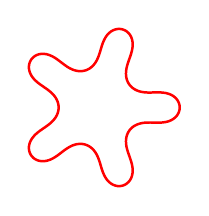
\begin{tikzpicture}[scale=0.45]

  \begin{axis}[
    hide axis,
    axis equal image,
    xmin = -1.42,
    xmax = 1.42,
    ymin = -1.42,
    ymax = 1.42,
    xtick = \empty,
    ytick = \empty,
    title style={align=left},
%    title={\Large $t = 2.99 \times 10^{-2}$ \\ \\ \Large $\nu = 0.38$}
  ]

\addplot[red,line width=2pt] coordinates{
(1.1542e+00,-1.5683e-12)
(1.1521e+00,2.7715e-02)
(1.1455e+00,5.5460e-02)
(1.1342e+00,8.3060e-02)
(1.1178e+00,1.1001e-01)
(1.0958e+00,1.3550e-01)
(1.0683e+00,1.5849e-01)
(1.0358e+00,1.7798e-01)
(9.9887e-01,1.9322e-01)
(9.5866e-01,2.0389e-01)
(9.1618e-01,2.1021e-01)
(8.7237e-01,2.1289e-01)
(8.2802e-01,2.1300e-01)
(7.8370e-01,2.1188e-01)
(7.3992e-01,2.1090e-01)
(6.9718e-01,2.1133e-01)
(6.5612e-01,2.1417e-01)
(6.1746e-01,2.2002e-01)
(5.8201e-01,2.2898e-01)
(5.5047e-01,2.4064e-01)
(5.2334e-01,2.5420e-01)
(5.0081e-01,2.6862e-01)
(4.8274e-01,2.8284e-01)
(4.6868e-01,2.9600e-01)
(4.5795e-01,3.0761e-01)
(4.4962e-01,3.1777e-01)
(4.4254e-01,3.2742e-01)
(4.3553e-01,3.3808e-01)
(4.2794e-01,3.5124e-01)
(4.1981e-01,3.6790e-01)
(4.1176e-01,3.8863e-01)
(4.0468e-01,4.1366e-01)
(3.9964e-01,4.4286e-01)
(3.9760e-01,4.7578e-01)
(3.9926e-01,5.1176e-01)
(4.0486e-01,5.4998e-01)
(4.1418e-01,5.8969e-01)
(4.2649e-01,6.3032e-01)
(4.4073e-01,6.7156e-01)
(4.5554e-01,7.1327e-01)
(4.6949e-01,7.5542e-01)
(4.8111e-01,7.9787e-01)
(4.8909e-01,8.4030e-01)
(4.9239e-01,8.8207e-01)
(4.9039e-01,9.2230e-01)
(4.8297e-01,9.5992e-01)
(4.7051e-01,9.9397e-01)
(4.5380e-01,1.0237e+00)
(4.3380e-01,1.0486e+00)
(4.1143e-01,1.0688e+00)
(3.8735e-01,1.0845e+00)
(3.6191e-01,1.0959e+00)
(3.3516e-01,1.1033e+00)
(3.0704e-01,1.1065e+00)
(2.7755e-01,1.1052e+00)
(2.4697e-01,1.0990e+00)
(2.1593e-01,1.0871e+00)
(1.8536e-01,1.0693e+00)
(1.5633e-01,1.0455e+00)
(1.2983e-01,1.0162e+00)
(1.0657e-01,9.8205e-01)
(8.6754e-02,9.4421e-01)
(7.0115e-02,9.0377e-01)
(5.5924e-02,8.6180e-01)
(4.3149e-02,8.1930e-01)
(3.0636e-02,7.7718e-01)
(1.7298e-02,7.3631e-01)
(2.3040e-03,6.9759e-01)
(-1.4778e-02,6.6193e-01)
(-3.3895e-02,6.3012e-01)
(-5.4525e-02,6.0278e-01)
(-7.5796e-02,5.8022e-01)
(-9.6673e-02,5.6235e-01)
(-1.1616e-01,5.4877e-01)
(-1.3351e-01,5.3883e-01)
(-1.4836e-01,5.3174e-01)
(-1.6095e-01,5.2666e-01)
(-1.7236e-01,5.2276e-01)
(-1.8433e-01,5.1934e-01)
(-1.9858e-01,5.1613e-01)
(-2.1619e-01,5.1339e-01)
(-2.3762e-01,5.1180e-01)
(-2.6288e-01,5.1228e-01)
(-2.9158e-01,5.1579e-01)
(-3.2307e-01,5.2317e-01)
(-3.5650e-01,5.3496e-01)
(-3.9099e-01,5.5123e-01)
(-4.2586e-01,5.7162e-01)
(-4.6072e-01,5.9535e-01)
(-4.9553e-01,6.2132e-01)
(-5.3053e-01,6.4828e-01)
(-5.6614e-01,6.7481e-01)
(-6.0270e-01,6.9952e-01)
(-6.4038e-01,7.2102e-01)
(-6.7896e-01,7.3808e-01)
(-7.1787e-01,7.4976e-01)
(-7.5619e-01,7.5553e-01)
(-7.9288e-01,7.5536e-01)
(-8.2692e-01,7.4966e-01)
(-8.5758e-01,7.3921e-01)
(-8.8447e-01,7.2485e-01)
(-9.0755e-01,7.0735e-01)
(-9.2697e-01,6.8718e-01)
(-9.4291e-01,6.6451e-01)
(-9.5538e-01,6.3929e-01)
(-9.6411e-01,6.1140e-01)
(-9.6854e-01,5.8087e-01)
(-9.6795e-01,5.4807e-01)
(-9.6166e-01,5.1369e-01)
(-9.4925e-01,4.7872e-01)
(-9.3072e-01,4.4424e-01)
(-9.0651e-01,4.1119e-01)
(-8.7748e-01,3.8021e-01)
(-8.4475e-01,3.5146e-01)
(-8.0956e-01,3.2467e-01)
(-7.7318e-01,2.9922e-01)
(-7.3683e-01,2.7429e-01)
(-7.0170e-01,2.4911e-01)
(-6.6892e-01,2.2309e-01)
(-6.3950e-01,1.9602e-01)
(-6.1425e-01,1.6811e-01)
(-5.9367e-01,1.3999e-01)
(-5.7786e-01,1.1254e-01)
(-5.6649e-01,8.6721e-02)
(-5.5894e-01,6.3407e-02)
(-5.5435e-01,4.3180e-02)
(-5.5187e-01,2.6233e-02)
(-5.5074e-01,1.2209e-02)
(-5.5043e-01,1.8275e-12)
(-5.5074e-01,-1.2209e-02)
(-5.5187e-01,-2.6233e-02)
(-5.5435e-01,-4.3180e-02)
(-5.5894e-01,-6.3407e-02)
(-5.6649e-01,-8.6721e-02)
(-5.7786e-01,-1.1254e-01)
(-5.9367e-01,-1.3999e-01)
(-6.1425e-01,-1.6811e-01)
(-6.3950e-01,-1.9602e-01)
(-6.6892e-01,-2.2309e-01)
(-7.0170e-01,-2.4911e-01)
(-7.3683e-01,-2.7429e-01)
(-7.7318e-01,-2.9922e-01)
(-8.0956e-01,-3.2467e-01)
(-8.4475e-01,-3.5146e-01)
(-8.7748e-01,-3.8021e-01)
(-9.0651e-01,-4.1119e-01)
(-9.3072e-01,-4.4424e-01)
(-9.4925e-01,-4.7872e-01)
(-9.6166e-01,-5.1369e-01)
(-9.6795e-01,-5.4807e-01)
(-9.6854e-01,-5.8087e-01)
(-9.6411e-01,-6.1140e-01)
(-9.5538e-01,-6.3929e-01)
(-9.4291e-01,-6.6451e-01)
(-9.2697e-01,-6.8718e-01)
(-9.0755e-01,-7.0735e-01)
(-8.8447e-01,-7.2485e-01)
(-8.5758e-01,-7.3921e-01)
(-8.2692e-01,-7.4966e-01)
(-7.9288e-01,-7.5536e-01)
(-7.5619e-01,-7.5553e-01)
(-7.1787e-01,-7.4976e-01)
(-6.7896e-01,-7.3808e-01)
(-6.4038e-01,-7.2102e-01)
(-6.0270e-01,-6.9952e-01)
(-5.6614e-01,-6.7481e-01)
(-5.3053e-01,-6.4828e-01)
(-4.9553e-01,-6.2132e-01)
(-4.6072e-01,-5.9535e-01)
(-4.2586e-01,-5.7162e-01)
(-3.9099e-01,-5.5123e-01)
(-3.5650e-01,-5.3496e-01)
(-3.2307e-01,-5.2317e-01)
(-2.9158e-01,-5.1579e-01)
(-2.6288e-01,-5.1228e-01)
(-2.3762e-01,-5.1180e-01)
(-2.1619e-01,-5.1339e-01)
(-1.9858e-01,-5.1613e-01)
(-1.8433e-01,-5.1934e-01)
(-1.7236e-01,-5.2276e-01)
(-1.6095e-01,-5.2666e-01)
(-1.4836e-01,-5.3174e-01)
(-1.3351e-01,-5.3883e-01)
(-1.1616e-01,-5.4877e-01)
(-9.6673e-02,-5.6235e-01)
(-7.5796e-02,-5.8022e-01)
(-5.4525e-02,-6.0278e-01)
(-3.3895e-02,-6.3012e-01)
(-1.4778e-02,-6.6193e-01)
(2.3040e-03,-6.9759e-01)
(1.7298e-02,-7.3631e-01)
(3.0636e-02,-7.7718e-01)
(4.3149e-02,-8.1930e-01)
(5.5924e-02,-8.6180e-01)
(7.0115e-02,-9.0377e-01)
(8.6754e-02,-9.4421e-01)
(1.0657e-01,-9.8205e-01)
(1.2983e-01,-1.0162e+00)
(1.5633e-01,-1.0455e+00)
(1.8536e-01,-1.0693e+00)
(2.1593e-01,-1.0871e+00)
(2.4697e-01,-1.0990e+00)
(2.7755e-01,-1.1052e+00)
(3.0704e-01,-1.1065e+00)
(3.3516e-01,-1.1033e+00)
(3.6191e-01,-1.0959e+00)
(3.8735e-01,-1.0845e+00)
(4.1143e-01,-1.0688e+00)
(4.3380e-01,-1.0486e+00)
(4.5380e-01,-1.0237e+00)
(4.7051e-01,-9.9397e-01)
(4.8297e-01,-9.5992e-01)
(4.9039e-01,-9.2230e-01)
(4.9239e-01,-8.8207e-01)
(4.8909e-01,-8.4030e-01)
(4.8111e-01,-7.9787e-01)
(4.6949e-01,-7.5542e-01)
(4.5554e-01,-7.1327e-01)
(4.4073e-01,-6.7156e-01)
(4.2649e-01,-6.3032e-01)
(4.1418e-01,-5.8969e-01)
(4.0486e-01,-5.4998e-01)
(3.9926e-01,-5.1176e-01)
(3.9760e-01,-4.7578e-01)
(3.9964e-01,-4.4286e-01)
(4.0468e-01,-4.1366e-01)
(4.1176e-01,-3.8863e-01)
(4.1981e-01,-3.6790e-01)
(4.2794e-01,-3.5124e-01)
(4.3553e-01,-3.3808e-01)
(4.4254e-01,-3.2742e-01)
(4.4962e-01,-3.1777e-01)
(4.5795e-01,-3.0761e-01)
(4.6868e-01,-2.9600e-01)
(4.8274e-01,-2.8284e-01)
(5.0081e-01,-2.6862e-01)
(5.2334e-01,-2.5420e-01)
(5.5047e-01,-2.4064e-01)
(5.8201e-01,-2.2898e-01)
(6.1746e-01,-2.2002e-01)
(6.5612e-01,-2.1417e-01)
(6.9718e-01,-2.1133e-01)
(7.3992e-01,-2.1090e-01)
(7.8370e-01,-2.1188e-01)
(8.2802e-01,-2.1300e-01)
(8.7237e-01,-2.1289e-01)
(9.1618e-01,-2.1021e-01)
(9.5866e-01,-2.0389e-01)
(9.9887e-01,-1.9322e-01)
(1.0358e+00,-1.7798e-01)
(1.0683e+00,-1.5849e-01)
(1.0958e+00,-1.3550e-01)
(1.1178e+00,-1.1001e-01)
(1.1342e+00,-8.3060e-02)
(1.1455e+00,-5.5460e-02)
(1.1521e+00,-2.7715e-02)
(1.1542e+00,-1.5683e-12)
};


\end{axis}

\end{tikzpicture}

%    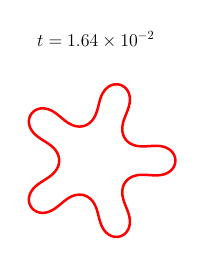
\begin{tikzpicture}[scale=0.45]

  \begin{axis}[
    hide axis,
    axis equal image,
    xmin = -2.1,
    xmax = 2.1,
    ymin = -2.1,
    ymax = 2.1,
    xtick = \empty,
    ytick = \empty,
    title style={align=left},
    title={\Large $t = 1.64 \times 10^{-2}$}
  ]

\addplot[red,line width=2pt] coordinates{
(1.6571e+00,-2.4995e-13)
(1.6540e+00,4.0568e-02)
(1.6446e+00,8.1200e-02)
(1.6282e+00,1.2166e-01)
(1.6043e+00,1.6121e-01)
(1.5722e+00,1.9863e-01)
(1.5321e+00,2.3234e-01)
(1.4844e+00,2.6078e-01)
(1.4303e+00,2.8269e-01)
(1.3712e+00,2.9752e-01)
(1.3088e+00,3.0550e-01)
(1.2447e+00,3.0765e-01)
(1.1798e+00,3.0562e-01)
(1.1150e+00,3.0146e-01)
(1.0511e+00,2.9730e-01)
(9.8855e-01,2.9516e-01)
(9.2832e-01,2.9667e-01)
(8.7143e-01,3.0283e-01)
(8.1907e-01,3.1391e-01)
(7.7235e-01,3.2939e-01)
(7.3210e-01,3.4809e-01)
(6.9865e-01,3.6843e-01)
(6.7184e-01,3.8879e-01)
(6.5103e-01,4.0781e-01)
(6.3518e-01,4.2470e-01)
(6.2292e-01,4.3956e-01)
(6.1255e-01,4.5367e-01)
(6.0232e-01,4.6933e-01)
(5.9132e-01,4.8869e-01)
(5.7970e-01,5.1321e-01)
(5.6840e-01,5.4374e-01)
(5.5884e-01,5.8058e-01)
(5.5264e-01,6.2350e-01)
(5.5125e-01,6.7177e-01)
(5.5567e-01,7.2429e-01)
(5.6620e-01,7.7984e-01)
(5.8238e-01,8.3730e-01)
(6.0302e-01,8.9592e-01)
(6.2643e-01,9.5532e-01)
(6.5053e-01,1.0155e+00)
(6.7308e-01,1.0764e+00)
(6.9187e-01,1.1380e+00)
(7.0491e-01,1.1998e+00)
(7.1065e-01,1.2609e+00)
(7.0821e-01,1.3198e+00)
(6.9750e-01,1.3749e+00)
(6.7921e-01,1.4247e+00)
(6.5461e-01,1.4681e+00)
(6.2519e-01,1.5045e+00)
(5.9232e-01,1.5339e+00)
(5.5701e-01,1.5567e+00)
(5.1976e-01,1.5734e+00)
(4.8061e-01,1.5842e+00)
(4.3946e-01,1.5890e+00)
(3.9629e-01,1.5873e+00)
(3.5151e-01,1.5783e+00)
(3.0601e-01,1.5611e+00)
(2.6120e-01,1.5352e+00)
(2.1875e-01,1.5003e+00)
(1.8023e-01,1.4572e+00)
(1.4679e-01,1.4068e+00)
(1.1886e-01,1.3509e+00)
(9.6059e-02,1.2911e+00)
(7.7305e-02,1.2290e+00)
(6.0987e-02,1.1662e+00)
(4.5272e-02,1.1038e+00)
(2.8403e-02,1.0432e+00)
(8.9895e-03,9.8560e-01)
(-1.3754e-02,9.3237e-01)
(-3.9864e-02,8.8474e-01)
(-6.8632e-02,8.4370e-01)
(-9.8765e-02,8.0976e-01)
(-1.2869e-01,7.8288e-01)
(-1.5685e-01,7.6249e-01)
(-1.8205e-01,7.4761e-01)
(-2.0372e-01,7.3704e-01)
(-2.2214e-01,7.2952e-01)
(-2.3883e-01,7.2379e-01)
(-2.5638e-01,7.1883e-01)
(-2.7730e-01,7.1424e-01)
(-3.0312e-01,7.1049e-01)
(-3.3453e-01,7.0863e-01)
(-3.7147e-01,7.1008e-01)
(-4.1334e-01,7.1633e-01)
(-4.5905e-01,7.2861e-01)
(-5.0730e-01,7.4766e-01)
(-5.5676e-01,7.7353e-01)
(-6.0644e-01,8.0557e-01)
(-6.5587e-01,8.4253e-01)
(-7.0512e-01,8.8272e-01)
(-7.5471e-01,9.2421e-01)
(-8.0539e-01,9.6491e-01)
(-8.5779e-01,1.0027e+00)
(-9.1218e-01,1.0354e+00)
(-9.6824e-01,1.0613e+00)
(-1.0250e+00,1.0789e+00)
(-1.0811e+00,1.0876e+00)
(-1.1348e+00,1.0873e+00)
(-1.1845e+00,1.0788e+00)
(-1.2294e+00,1.0633e+00)
(-1.2686e+00,1.0422e+00)
(-1.3023e+00,1.0164e+00)
(-1.3307e+00,9.8687e-01)
(-1.3541e+00,9.5370e-01)
(-1.3724e+00,9.1682e-01)
(-1.3853e+00,8.7603e-01)
(-1.3920e+00,8.3139e-01)
(-1.3913e+00,7.8337e-01)
(-1.3822e+00,7.3304e-01)
(-1.3640e+00,6.8186e-01)
(-1.3367e+00,6.3152e-01)
(-1.3007e+00,5.8355e-01)
(-1.2574e+00,5.3896e-01)
(-1.2085e+00,4.9808e-01)
(-1.1558e+00,4.6051e-01)
(-1.1012e+00,4.2525e-01)
(-1.0466e+00,3.9099e-01)
(-9.9359e-01,3.5642e-01)
(-9.4396e-01,3.2051e-01)
(-8.9923e-01,2.8279e-01)
(-8.6065e-01,2.4347e-01)
(-8.2907e-01,2.0343e-01)
(-8.0469e-01,1.6398e-01)
(-7.8711e-01,1.2663e-01)
(-7.7539e-01,9.2723e-02)
(-7.6827e-01,6.3215e-02)
(-7.6441e-01,3.8427e-02)
(-7.6264e-01,1.7877e-02)
(-7.6216e-01,-1.0277e-13)
(-7.6264e-01,-1.7877e-02)
(-7.6441e-01,-3.8427e-02)
(-7.6827e-01,-6.3215e-02)
(-7.7539e-01,-9.2723e-02)
(-7.8711e-01,-1.2663e-01)
(-8.0469e-01,-1.6398e-01)
(-8.2907e-01,-2.0343e-01)
(-8.6065e-01,-2.4347e-01)
(-8.9923e-01,-2.8279e-01)
(-9.4396e-01,-3.2051e-01)
(-9.9359e-01,-3.5642e-01)
(-1.0466e+00,-3.9099e-01)
(-1.1012e+00,-4.2525e-01)
(-1.1558e+00,-4.6051e-01)
(-1.2085e+00,-4.9808e-01)
(-1.2574e+00,-5.3896e-01)
(-1.3007e+00,-5.8355e-01)
(-1.3367e+00,-6.3152e-01)
(-1.3640e+00,-6.8186e-01)
(-1.3822e+00,-7.3304e-01)
(-1.3913e+00,-7.8337e-01)
(-1.3920e+00,-8.3139e-01)
(-1.3853e+00,-8.7603e-01)
(-1.3724e+00,-9.1682e-01)
(-1.3541e+00,-9.5370e-01)
(-1.3307e+00,-9.8687e-01)
(-1.3023e+00,-1.0164e+00)
(-1.2686e+00,-1.0422e+00)
(-1.2294e+00,-1.0633e+00)
(-1.1845e+00,-1.0788e+00)
(-1.1348e+00,-1.0873e+00)
(-1.0811e+00,-1.0876e+00)
(-1.0250e+00,-1.0789e+00)
(-9.6824e-01,-1.0613e+00)
(-9.1218e-01,-1.0354e+00)
(-8.5779e-01,-1.0027e+00)
(-8.0539e-01,-9.6491e-01)
(-7.5471e-01,-9.2421e-01)
(-7.0512e-01,-8.8272e-01)
(-6.5587e-01,-8.4253e-01)
(-6.0644e-01,-8.0557e-01)
(-5.5676e-01,-7.7353e-01)
(-5.0730e-01,-7.4766e-01)
(-4.5905e-01,-7.2861e-01)
(-4.1334e-01,-7.1633e-01)
(-3.7147e-01,-7.1008e-01)
(-3.3453e-01,-7.0863e-01)
(-3.0312e-01,-7.1049e-01)
(-2.7730e-01,-7.1424e-01)
(-2.5638e-01,-7.1883e-01)
(-2.3883e-01,-7.2379e-01)
(-2.2214e-01,-7.2952e-01)
(-2.0372e-01,-7.3704e-01)
(-1.8205e-01,-7.4761e-01)
(-1.5685e-01,-7.6249e-01)
(-1.2869e-01,-7.8288e-01)
(-9.8765e-02,-8.0976e-01)
(-6.8632e-02,-8.4370e-01)
(-3.9864e-02,-8.8474e-01)
(-1.3754e-02,-9.3237e-01)
(8.9895e-03,-9.8560e-01)
(2.8403e-02,-1.0432e+00)
(4.5272e-02,-1.1038e+00)
(6.0987e-02,-1.1662e+00)
(7.7305e-02,-1.2290e+00)
(9.6059e-02,-1.2911e+00)
(1.1886e-01,-1.3509e+00)
(1.4679e-01,-1.4068e+00)
(1.8023e-01,-1.4572e+00)
(2.1875e-01,-1.5003e+00)
(2.6120e-01,-1.5352e+00)
(3.0601e-01,-1.5611e+00)
(3.5151e-01,-1.5783e+00)
(3.9629e-01,-1.5873e+00)
(4.3946e-01,-1.5890e+00)
(4.8061e-01,-1.5842e+00)
(5.1976e-01,-1.5734e+00)
(5.5701e-01,-1.5567e+00)
(5.9232e-01,-1.5339e+00)
(6.2519e-01,-1.5045e+00)
(6.5461e-01,-1.4681e+00)
(6.7921e-01,-1.4247e+00)
(6.9750e-01,-1.3749e+00)
(7.0821e-01,-1.3198e+00)
(7.1065e-01,-1.2609e+00)
(7.0491e-01,-1.1998e+00)
(6.9187e-01,-1.1380e+00)
(6.7308e-01,-1.0764e+00)
(6.5053e-01,-1.0155e+00)
(6.2643e-01,-9.5532e-01)
(6.0302e-01,-8.9592e-01)
(5.8238e-01,-8.3730e-01)
(5.6620e-01,-7.7984e-01)
(5.5567e-01,-7.2429e-01)
(5.5125e-01,-6.7177e-01)
(5.5264e-01,-6.2350e-01)
(5.5884e-01,-5.8058e-01)
(5.6840e-01,-5.4374e-01)
(5.7970e-01,-5.1321e-01)
(5.9132e-01,-4.8869e-01)
(6.0232e-01,-4.6933e-01)
(6.1255e-01,-4.5367e-01)
(6.2292e-01,-4.3956e-01)
(6.3518e-01,-4.2470e-01)
(6.5103e-01,-4.0781e-01)
(6.7184e-01,-3.8879e-01)
(6.9865e-01,-3.6843e-01)
(7.3210e-01,-3.4809e-01)
(7.7235e-01,-3.2939e-01)
(8.1907e-01,-3.1391e-01)
(8.7143e-01,-3.0283e-01)
(9.2832e-01,-2.9667e-01)
(9.8855e-01,-2.9516e-01)
(1.0511e+00,-2.9730e-01)
(1.1150e+00,-3.0146e-01)
(1.1798e+00,-3.0562e-01)
(1.2447e+00,-3.0765e-01)
(1.3088e+00,-3.0550e-01)
(1.3712e+00,-2.9752e-01)
(1.4303e+00,-2.8269e-01)
(1.4844e+00,-2.6078e-01)
(1.5321e+00,-2.3234e-01)
(1.5722e+00,-1.9863e-01)
(1.6043e+00,-1.6121e-01)
(1.6282e+00,-1.2166e-01)
(1.6446e+00,-8.1200e-02)
(1.6540e+00,-4.0568e-02)
(1.6571e+00,-2.4995e-13)
};



\end{axis}

\end{tikzpicture}

%    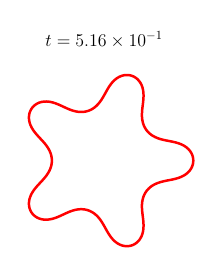
\begin{tikzpicture}[scale=0.45]

  \begin{axis}[
    hide axis,
    axis equal image,
    xmin = -2.1,
    xmax = 2.1,
    ymin = -2.1,
    ymax = 2.1,
    xtick = \empty,
    ytick = \empty,
    title style={align=left},
    title={\Large $t = 5.16 \times 10^{-1}$}
  ]

\addplot[red,line width=2pt] coordinates{
(1.8573e+00,-9.0339e-12)
(1.8547e+00,4.0614e-02)
(1.8468e+00,8.1577e-02)
(1.8329e+00,1.2298e-01)
(1.8125e+00,1.6450e-01)
(1.7849e+00,2.0534e-01)
(1.7499e+00,2.4438e-01)
(1.7076e+00,2.8039e-01)
(1.6587e+00,3.1229e-01)
(1.6042e+00,3.3941e-01)
(1.5454e+00,3.6165e-01)
(1.4837e+00,3.7953e-01)
(1.4204e+00,3.9408e-01)
(1.3568e+00,4.0669e-01)
(1.2938e+00,4.1888e-01)
(1.2327e+00,4.3205e-01)
(1.1744e+00,4.4730e-01)
(1.1200e+00,4.6519e-01)
(1.0706e+00,4.8573e-01)
(1.0269e+00,5.0836e-01)
(9.8935e-01,5.3209e-01)
(9.5812e-01,5.5570e-01)
(9.3291e-01,5.7802e-01)
(9.1310e-01,5.9809e-01)
(8.9780e-01,6.1548e-01)
(8.8578e-01,6.3053e-01)
(8.7542e-01,6.4466e-01)
(8.6500e-01,6.6019e-01)
(8.5345e-01,6.7922e-01)
(8.4067e-01,7.0316e-01)
(8.2726e-01,7.3284e-01)
(8.1423e-01,7.6861e-01)
(8.0279e-01,8.1045e-01)
(7.9411e-01,8.5796e-01)
(7.8906e-01,9.1044e-01)
(7.8804e-01,9.6697e-01)
(7.9086e-01,1.0266e+00)
(7.9675e-01,1.0885e+00)
(8.0444e-01,1.1519e+00)
(8.1229e-01,1.2162e+00)
(8.1853e-01,1.2808e+00)
(8.2145e-01,1.3452e+00)
(8.1957e-01,1.4084e+00)
(8.1186e-01,1.4692e+00)
(7.9790e-01,1.5265e+00)
(7.7786e-01,1.5789e+00)
(7.5249e-01,1.6256e+00)
(7.2287e-01,1.6657e+00)
(6.9018e-01,1.6993e+00)
(6.5541e-01,1.7264e+00)
(6.1917e-01,1.7478e+00)
(5.8162e-01,1.7638e+00)
(5.4255e-01,1.7749e+00)
(5.0156e-01,1.7810e+00)
(4.5835e-01,1.7817e+00)
(4.1296e-01,1.7765e+00)
(3.6585e-01,1.7643e+00)
(3.1792e-01,1.7447e+00)
(2.7038e-01,1.7172e+00)
(2.2445e-01,1.6819e+00)
(1.8119e-01,1.6397e+00)
(1.4119e-01,1.5917e+00)
(1.0450e-01,1.5392e+00)
(7.0641e-02,1.4839e+00)
(3.8719e-02,1.4274e+00)
(7.6439e-03,1.3711e+00)
(-2.3635e-02,1.3165e+00)
(-5.5892e-02,1.2650e+00)
(-8.9454e-02,1.2178e+00)
(-1.2412e-01,1.1760e+00)
(-1.5918e-01,1.1401e+00)
(-1.9361e-01,1.1105e+00)
(-2.2623e-01,1.0870e+00)
(-2.5593e-01,1.0689e+00)
(-2.8193e-01,1.0555e+00)
(-3.0396e-01,1.0457e+00)
(-3.2253e-01,1.0385e+00)
(-3.3924e-01,1.0328e+00)
(-3.5674e-01,1.0277e+00)
(-3.7754e-01,1.0226e+00)
(-4.0318e-01,1.0177e+00)
(-4.3440e-01,1.0138e+00)
(-4.7133e-01,1.0119e+00)
(-5.1365e-01,1.0132e+00)
(-5.6068e-01,1.0187e+00)
(-6.1151e-01,1.0291e+00)
(-6.6515e-01,1.0446e+00)
(-7.2070e-01,1.0648e+00)
(-7.7752e-01,1.0890e+00)
(-8.3526e-01,1.1155e+00)
(-8.9383e-01,1.1429e+00)
(-9.5324e-01,1.1693e+00)
(-1.0134e+00,1.1928e+00)
(-1.0741e+00,1.2116e+00)
(-1.1345e+00,1.2244e+00)
(-1.1936e+00,1.2303e+00)
(-1.2504e+00,1.2289e+00)
(-1.3034e+00,1.2204e+00)
(-1.3518e+00,1.2058e+00)
(-1.3949e+00,1.1860e+00)
(-1.4325e+00,1.1620e+00)
(-1.4650e+00,1.1348e+00)
(-1.4927e+00,1.1046e+00)
(-1.5161e+00,1.0715e+00)
(-1.5355e+00,1.0351e+00)
(-1.5505e+00,9.9499e-01)
(-1.5606e+00,9.5098e-01)
(-1.5649e+00,9.0314e-01)
(-1.5624e+00,8.5203e-01)
(-1.5525e+00,7.9862e-01)
(-1.5347e+00,7.4413e-01)
(-1.5094e+00,6.8978e-01)
(-1.4773e+00,6.3657e-01)
(-1.4397e+00,5.8510e-01)
(-1.3981e+00,5.3547e-01)
(-1.3544e+00,4.8738e-01)
(-1.3103e+00,4.4029e-01)
(-1.2676e+00,3.9364e-01)
(-1.2278e+00,3.4705e-01)
(-1.1923e+00,3.0051e-01)
(-1.1621e+00,2.5444e-01)
(-1.1377e+00,2.0964e-01)
(-1.1191e+00,1.6716e-01)
(-1.1058e+00,1.2807e-01)
(-1.0970e+00,9.3280e-02)
(-1.0917e+00,6.3390e-02)
(-1.0888e+00,3.8466e-02)
(-1.0875e+00,1.7880e-02)
(-1.0871e+00,1.1759e-11)
(-1.0875e+00,-1.7880e-02)
(-1.0888e+00,-3.8466e-02)
(-1.0917e+00,-6.3390e-02)
(-1.0970e+00,-9.3280e-02)
(-1.1058e+00,-1.2807e-01)
(-1.1191e+00,-1.6716e-01)
(-1.1377e+00,-2.0964e-01)
(-1.1621e+00,-2.5444e-01)
(-1.1923e+00,-3.0051e-01)
(-1.2278e+00,-3.4705e-01)
(-1.2676e+00,-3.9364e-01)
(-1.3103e+00,-4.4029e-01)
(-1.3544e+00,-4.8738e-01)
(-1.3981e+00,-5.3547e-01)
(-1.4397e+00,-5.8510e-01)
(-1.4773e+00,-6.3657e-01)
(-1.5094e+00,-6.8978e-01)
(-1.5347e+00,-7.4413e-01)
(-1.5525e+00,-7.9862e-01)
(-1.5624e+00,-8.5203e-01)
(-1.5649e+00,-9.0314e-01)
(-1.5606e+00,-9.5098e-01)
(-1.5505e+00,-9.9499e-01)
(-1.5355e+00,-1.0351e+00)
(-1.5161e+00,-1.0715e+00)
(-1.4927e+00,-1.1046e+00)
(-1.4650e+00,-1.1348e+00)
(-1.4325e+00,-1.1620e+00)
(-1.3949e+00,-1.1860e+00)
(-1.3518e+00,-1.2058e+00)
(-1.3034e+00,-1.2204e+00)
(-1.2504e+00,-1.2289e+00)
(-1.1936e+00,-1.2303e+00)
(-1.1345e+00,-1.2244e+00)
(-1.0741e+00,-1.2116e+00)
(-1.0134e+00,-1.1928e+00)
(-9.5324e-01,-1.1693e+00)
(-8.9383e-01,-1.1429e+00)
(-8.3526e-01,-1.1155e+00)
(-7.7752e-01,-1.0890e+00)
(-7.2070e-01,-1.0648e+00)
(-6.6515e-01,-1.0446e+00)
(-6.1151e-01,-1.0291e+00)
(-5.6068e-01,-1.0187e+00)
(-5.1365e-01,-1.0132e+00)
(-4.7133e-01,-1.0119e+00)
(-4.3440e-01,-1.0138e+00)
(-4.0318e-01,-1.0177e+00)
(-3.7754e-01,-1.0226e+00)
(-3.5674e-01,-1.0277e+00)
(-3.3924e-01,-1.0328e+00)
(-3.2253e-01,-1.0385e+00)
(-3.0396e-01,-1.0457e+00)
(-2.8193e-01,-1.0555e+00)
(-2.5593e-01,-1.0689e+00)
(-2.2623e-01,-1.0870e+00)
(-1.9361e-01,-1.1105e+00)
(-1.5918e-01,-1.1401e+00)
(-1.2412e-01,-1.1760e+00)
(-8.9454e-02,-1.2178e+00)
(-5.5892e-02,-1.2650e+00)
(-2.3635e-02,-1.3165e+00)
(7.6439e-03,-1.3711e+00)
(3.8719e-02,-1.4274e+00)
(7.0641e-02,-1.4839e+00)
(1.0450e-01,-1.5392e+00)
(1.4119e-01,-1.5917e+00)
(1.8119e-01,-1.6397e+00)
(2.2445e-01,-1.6819e+00)
(2.7038e-01,-1.7172e+00)
(3.1792e-01,-1.7447e+00)
(3.6585e-01,-1.7643e+00)
(4.1296e-01,-1.7765e+00)
(4.5835e-01,-1.7817e+00)
(5.0156e-01,-1.7810e+00)
(5.4255e-01,-1.7749e+00)
(5.8162e-01,-1.7638e+00)
(6.1917e-01,-1.7478e+00)
(6.5541e-01,-1.7264e+00)
(6.9018e-01,-1.6993e+00)
(7.2287e-01,-1.6657e+00)
(7.5249e-01,-1.6256e+00)
(7.7786e-01,-1.5789e+00)
(7.9790e-01,-1.5265e+00)
(8.1186e-01,-1.4692e+00)
(8.1957e-01,-1.4084e+00)
(8.2145e-01,-1.3452e+00)
(8.1853e-01,-1.2808e+00)
(8.1229e-01,-1.2162e+00)
(8.0444e-01,-1.1519e+00)
(7.9675e-01,-1.0885e+00)
(7.9086e-01,-1.0266e+00)
(7.8804e-01,-9.6697e-01)
(7.8906e-01,-9.1044e-01)
(7.9411e-01,-8.5796e-01)
(8.0279e-01,-8.1045e-01)
(8.1423e-01,-7.6861e-01)
(8.2726e-01,-7.3284e-01)
(8.4067e-01,-7.0316e-01)
(8.5345e-01,-6.7922e-01)
(8.6500e-01,-6.6019e-01)
(8.7542e-01,-6.4466e-01)
(8.8578e-01,-6.3053e-01)
(8.9780e-01,-6.1548e-01)
(9.1310e-01,-5.9809e-01)
(9.3291e-01,-5.7802e-01)
(9.5812e-01,-5.5570e-01)
(9.8935e-01,-5.3209e-01)
(1.0269e+00,-5.0836e-01)
(1.0706e+00,-4.8573e-01)
(1.1200e+00,-4.6519e-01)
(1.1744e+00,-4.4730e-01)
(1.2327e+00,-4.3205e-01)
(1.2938e+00,-4.1888e-01)
(1.3568e+00,-4.0669e-01)
(1.4204e+00,-3.9408e-01)
(1.4837e+00,-3.7953e-01)
(1.5454e+00,-3.6165e-01)
(1.6042e+00,-3.3941e-01)
(1.6587e+00,-3.1229e-01)
(1.7076e+00,-2.8039e-01)
(1.7499e+00,-2.4438e-01)
(1.7849e+00,-2.0534e-01)
(1.8125e+00,-1.6450e-01)
(1.8329e+00,-1.2298e-01)
(1.8468e+00,-8.1577e-02)
(1.8547e+00,-4.0614e-02)
(1.8573e+00,-9.0339e-12)
};



\end{axis}

\end{tikzpicture}

%    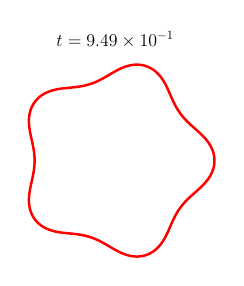
\begin{tikzpicture}[scale=0.45]

  \begin{axis}[
    hide axis,
    axis equal image,
    xmin = -2.1,
    xmax = 2.1,
    ymin = -2.1,
    ymax = 2.1,
    xtick = \empty,
    ytick = \empty,
    title style={align=left},
    title={\Large $t = 9.49 \times 10^{-1}$}
  ]

\addplot[red,line width=2pt] coordinates{
(2.0699e+00,-5.6473e-11)
(2.0685e+00,4.0691e-02)
(2.0641e+00,8.2211e-02)
(2.0564e+00,1.2521e-01)
(2.0450e+00,1.7005e-01)
(2.0292e+00,2.1674e-01)
(2.0085e+00,2.6499e-01)
(1.9828e+00,3.1424e-01)
(1.9519e+00,3.6386e-01)
(1.9161e+00,4.1317e-01)
(1.8760e+00,4.6160e-01)
(1.8324e+00,5.0875e-01)
(1.7863e+00,5.5443e-01)
(1.7387e+00,5.9859e-01)
(1.6909e+00,6.4131e-01)
(1.6440e+00,6.8270e-01)
(1.5990e+00,7.2276e-01)
(1.5568e+00,7.6141e-01)
(1.5181e+00,7.9839e-01)
(1.4833e+00,8.3329e-01)
(1.4529e+00,8.6561e-01)
(1.4268e+00,8.9485e-01)
(1.4051e+00,9.2056e-01)
(1.3873e+00,9.4249e-01)
(1.3731e+00,9.6079e-01)
(1.3616e+00,9.7620e-01)
(1.3513e+00,9.9036e-01)
(1.3405e+00,1.0056e+00)
(1.3279e+00,1.0240e+00)
(1.3130e+00,1.0467e+00)
(1.2957e+00,1.0743e+00)
(1.2763e+00,1.1071e+00)
(1.2553e+00,1.1450e+00)
(1.2330e+00,1.1879e+00)
(1.2099e+00,1.2353e+00)
(1.1863e+00,1.2867e+00)
(1.1622e+00,1.3413e+00)
(1.1375e+00,1.3984e+00)
(1.1119e+00,1.4568e+00)
(1.0849e+00,1.5157e+00)
(1.0561e+00,1.5740e+00)
(1.0252e+00,1.6305e+00)
(9.9198e-01,1.6843e+00)
(9.5655e-01,1.7344e+00)
(9.1923e-01,1.7800e+00)
(8.8054e-01,1.8208e+00)
(8.4111e-01,1.8563e+00)
(8.0155e-01,1.8868e+00)
(7.6235e-01,1.9125e+00)
(7.2371e-01,1.9338e+00)
(6.8552e-01,1.9515e+00)
(6.4734e-01,1.9660e+00)
(6.0845e-01,1.9777e+00)
(5.6801e-01,1.9869e+00)
(5.2528e-01,1.9935e+00)
(4.7970e-01,1.9971e+00)
(4.3103e-01,1.9972e+00)
(3.7934e-01,1.9934e+00)
(3.2500e-01,1.9851e+00)
(2.6860e-01,1.9720e+00)
(2.1083e-01,1.9542e+00)
(1.5243e-01,1.9318e+00)
(9.4027e-02,1.9056e+00)
(3.6168e-02,1.8763e+00)
(-2.0752e-02,1.8450e+00)
(-7.6433e-02,1.8129e+00)
(-1.3062e-01,1.7809e+00)
(-1.8303e-01,1.7501e+00)
(-2.3332e-01,1.7214e+00)
(-2.8103e-01,1.6954e+00)
(-3.2564e-01,1.6725e+00)
(-3.6659e-01,1.6529e+00)
(-4.0334e-01,1.6365e+00)
(-4.3548e-01,1.6232e+00)
(-4.6277e-01,1.6126e+00)
(-4.8543e-01,1.6043e+00)
(-5.0424e-01,1.5978e+00)
(-5.2100e-01,1.5923e+00)
(-5.3840e-01,1.5868e+00)
(-5.5893e-01,1.5807e+00)
(-5.8408e-01,1.5737e+00)
(-6.1457e-01,1.5660e+00)
(-6.5062e-01,1.5577e+00)
(-6.9215e-01,1.5494e+00)
(-7.3882e-01,1.5413e+00)
(-7.9018e-01,1.5339e+00)
(-8.4562e-01,1.5272e+00)
(-9.0443e-01,1.5210e+00)
(-9.6588e-01,1.5152e+00)
(-1.0291e+00,1.5090e+00)
(-1.0934e+00,1.5018e+00)
(-1.1578e+00,1.4929e+00)
(-1.2214e+00,1.4815e+00)
(-1.2832e+00,1.4672e+00)
(-1.3424e+00,1.4496e+00)
(-1.3982e+00,1.4288e+00)
(-1.4498e+00,1.4051e+00)
(-1.4967e+00,1.3790e+00)
(-1.5389e+00,1.3511e+00)
(-1.5763e+00,1.3219e+00)
(-1.6094e+00,1.2919e+00)
(-1.6387e+00,1.2612e+00)
(-1.6648e+00,1.2296e+00)
(-1.6884e+00,1.1966e+00)
(-1.7100e+00,1.1615e+00)
(-1.7298e+00,1.1236e+00)
(-1.7478e+00,1.0821e+00)
(-1.7635e+00,1.0367e+00)
(-1.7764e+00,9.8714e-01)
(-1.7860e+00,9.3364e-01)
(-1.7918e+00,8.7660e-01)
(-1.7935e+00,8.1664e-01)
(-1.7911e+00,7.5452e-01)
(-1.7849e+00,6.9105e-01)
(-1.7755e+00,6.2701e-01)
(-1.7637e+00,5.6310e-01)
(-1.7505e+00,4.9997e-01)
(-1.7368e+00,4.3821e-01)
(-1.7236e+00,3.7839e-01)
(-1.7115e+00,3.2111e-01)
(-1.7011e+00,2.6699e-01)
(-1.6927e+00,2.1666e-01)
(-1.6863e+00,1.7071e-01)
(-1.6818e+00,1.2966e-01)
(-1.6788e+00,9.3894e-02)
(-1.6770e+00,6.3583e-02)
(-1.6760e+00,3.8509e-02)
(-1.6755e+00,1.7885e-02)
(-1.6754e+00,-9.7486e-12)
(-1.6755e+00,-1.7885e-02)
(-1.6760e+00,-3.8509e-02)
(-1.6770e+00,-6.3583e-02)
(-1.6788e+00,-9.3894e-02)
(-1.6818e+00,-1.2966e-01)
(-1.6863e+00,-1.7071e-01)
(-1.6927e+00,-2.1666e-01)
(-1.7011e+00,-2.6699e-01)
(-1.7115e+00,-3.2111e-01)
(-1.7236e+00,-3.7839e-01)
(-1.7368e+00,-4.3821e-01)
(-1.7505e+00,-4.9997e-01)
(-1.7637e+00,-5.6310e-01)
(-1.7755e+00,-6.2701e-01)
(-1.7849e+00,-6.9105e-01)
(-1.7911e+00,-7.5452e-01)
(-1.7935e+00,-8.1664e-01)
(-1.7918e+00,-8.7660e-01)
(-1.7860e+00,-9.3364e-01)
(-1.7764e+00,-9.8714e-01)
(-1.7635e+00,-1.0367e+00)
(-1.7478e+00,-1.0821e+00)
(-1.7298e+00,-1.1236e+00)
(-1.7100e+00,-1.1615e+00)
(-1.6884e+00,-1.1966e+00)
(-1.6648e+00,-1.2296e+00)
(-1.6387e+00,-1.2612e+00)
(-1.6094e+00,-1.2919e+00)
(-1.5763e+00,-1.3219e+00)
(-1.5389e+00,-1.3511e+00)
(-1.4967e+00,-1.3790e+00)
(-1.4498e+00,-1.4051e+00)
(-1.3982e+00,-1.4288e+00)
(-1.3424e+00,-1.4496e+00)
(-1.2832e+00,-1.4672e+00)
(-1.2214e+00,-1.4815e+00)
(-1.1578e+00,-1.4929e+00)
(-1.0934e+00,-1.5018e+00)
(-1.0291e+00,-1.5090e+00)
(-9.6588e-01,-1.5152e+00)
(-9.0443e-01,-1.5210e+00)
(-8.4562e-01,-1.5272e+00)
(-7.9018e-01,-1.5339e+00)
(-7.3882e-01,-1.5413e+00)
(-6.9215e-01,-1.5494e+00)
(-6.5062e-01,-1.5577e+00)
(-6.1457e-01,-1.5660e+00)
(-5.8408e-01,-1.5737e+00)
(-5.5893e-01,-1.5807e+00)
(-5.3840e-01,-1.5868e+00)
(-5.2100e-01,-1.5923e+00)
(-5.0424e-01,-1.5978e+00)
(-4.8543e-01,-1.6043e+00)
(-4.6277e-01,-1.6126e+00)
(-4.3548e-01,-1.6232e+00)
(-4.0334e-01,-1.6365e+00)
(-3.6659e-01,-1.6529e+00)
(-3.2564e-01,-1.6725e+00)
(-2.8103e-01,-1.6954e+00)
(-2.3332e-01,-1.7214e+00)
(-1.8303e-01,-1.7501e+00)
(-1.3062e-01,-1.7809e+00)
(-7.6433e-02,-1.8129e+00)
(-2.0752e-02,-1.8450e+00)
(3.6168e-02,-1.8763e+00)
(9.4027e-02,-1.9056e+00)
(1.5243e-01,-1.9318e+00)
(2.1083e-01,-1.9542e+00)
(2.6860e-01,-1.9720e+00)
(3.2500e-01,-1.9851e+00)
(3.7934e-01,-1.9934e+00)
(4.3103e-01,-1.9972e+00)
(4.7970e-01,-1.9971e+00)
(5.2528e-01,-1.9935e+00)
(5.6801e-01,-1.9869e+00)
(6.0845e-01,-1.9777e+00)
(6.4734e-01,-1.9660e+00)
(6.8552e-01,-1.9515e+00)
(7.2371e-01,-1.9338e+00)
(7.6235e-01,-1.9125e+00)
(8.0155e-01,-1.8868e+00)
(8.4111e-01,-1.8563e+00)
(8.8054e-01,-1.8208e+00)
(9.1923e-01,-1.7800e+00)
(9.5655e-01,-1.7344e+00)
(9.9198e-01,-1.6843e+00)
(1.0252e+00,-1.6305e+00)
(1.0561e+00,-1.5740e+00)
(1.0849e+00,-1.5157e+00)
(1.1119e+00,-1.4568e+00)
(1.1375e+00,-1.3984e+00)
(1.1622e+00,-1.3413e+00)
(1.1863e+00,-1.2867e+00)
(1.2099e+00,-1.2353e+00)
(1.2330e+00,-1.1879e+00)
(1.2553e+00,-1.1450e+00)
(1.2763e+00,-1.1071e+00)
(1.2957e+00,-1.0743e+00)
(1.3130e+00,-1.0467e+00)
(1.3279e+00,-1.0240e+00)
(1.3405e+00,-1.0056e+00)
(1.3513e+00,-9.9036e-01)
(1.3616e+00,-9.7620e-01)
(1.3731e+00,-9.6079e-01)
(1.3873e+00,-9.4249e-01)
(1.4051e+00,-9.2056e-01)
(1.4268e+00,-8.9485e-01)
(1.4529e+00,-8.6561e-01)
(1.4833e+00,-8.3329e-01)
(1.5181e+00,-7.9839e-01)
(1.5568e+00,-7.6141e-01)
(1.5990e+00,-7.2276e-01)
(1.6440e+00,-6.8270e-01)
(1.6909e+00,-6.4131e-01)
(1.7387e+00,-5.9859e-01)
(1.7863e+00,-5.5443e-01)
(1.8324e+00,-5.0875e-01)
(1.8760e+00,-4.6160e-01)
(1.9161e+00,-4.1317e-01)
(1.9519e+00,-3.6386e-01)
(1.9828e+00,-3.1424e-01)
(2.0085e+00,-2.6499e-01)
(2.0292e+00,-2.1674e-01)
(2.0450e+00,-1.7005e-01)
(2.0564e+00,-1.2521e-01)
(2.0641e+00,-8.2211e-02)
(2.0685e+00,-4.0691e-02)
(2.0699e+00,-5.6473e-11)
};


\end{axis}

\end{tikzpicture}

%    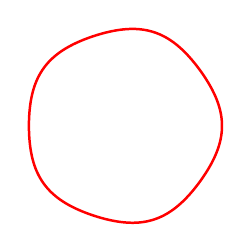
\begin{tikzpicture}[scale=0.45]

  \begin{axis}[
    hide axis,
    axis equal image,
    xmin = -1.42,
    xmax = 1.42,
    ymin = -1.42,
    ymax = 1.42,
    xtick = \empty,
    ytick = \empty,
    title style={align=left},
%    title={\Large $t = 3.17 \times 10^{-1}$ \\ \\ \Large $\nu = 0.99$}
  ]

\addplot[red,line width=2pt] coordinates{
(1.3864e+00,-4.3575e-10)
(1.3860e+00,2.7820e-02)
(1.3847e+00,5.6320e-02)
(1.3823e+00,8.6084e-02)
(1.3788e+00,1.1752e-01)
(1.3739e+00,1.5087e-01)
(1.3674e+00,1.8615e-01)
(1.3591e+00,2.2325e-01)
(1.3488e+00,2.6191e-01)
(1.3367e+00,3.0178e-01)
(1.3226e+00,3.4244e-01)
(1.3068e+00,3.8343e-01)
(1.2894e+00,4.2430e-01)
(1.2707e+00,4.6458e-01)
(1.2512e+00,5.0382e-01)
(1.2311e+00,5.4160e-01)
(1.2109e+00,5.7754e-01)
(1.1911e+00,6.1127e-01)
(1.1719e+00,6.4247e-01)
(1.1539e+00,6.7088e-01)
(1.1372e+00,6.9627e-01)
(1.1223e+00,7.1848e-01)
(1.1093e+00,7.3745e-01)
(1.0982e+00,7.5324e-01)
(1.0891e+00,7.6613e-01)
(1.0814e+00,7.7680e-01)
(1.0744e+00,7.8649e-01)
(1.0668e+00,7.9678e-01)
(1.0578e+00,8.0899e-01)
(1.0466e+00,8.2380e-01)
(1.0331e+00,8.4148e-01)
(1.0171e+00,8.6199e-01)
(9.9861e-01,8.8515e-01)
(9.7765e-01,9.1067e-01)
(9.5434e-01,9.3817e-01)
(9.2882e-01,9.6722e-01)
(9.0126e-01,9.9735e-01)
(8.7187e-01,1.0281e+00)
(8.4088e-01,1.0588e+00)
(8.0857e-01,1.0892e+00)
(7.7524e-01,1.1186e+00)
(7.4124e-01,1.1467e+00)
(7.0693e-01,1.1730e+00)
(6.7270e-01,1.1973e+00)
(6.3895e-01,1.2194e+00)
(6.0603e-01,1.2392e+00)
(5.7424e-01,1.2568e+00)
(5.4378e-01,1.2722e+00)
(5.1469e-01,1.2856e+00)
(4.8689e-01,1.2973e+00)
(4.6005e-01,1.3077e+00)
(4.3370e-01,1.3169e+00)
(4.0721e-01,1.3252e+00)
(3.7993e-01,1.3329e+00)
(3.5125e-01,1.3399e+00)
(3.2068e-01,1.3464e+00)
(2.8790e-01,1.3522e+00)
(2.5280e-01,1.3571e+00)
(2.1539e-01,1.3609e+00)
(1.7586e-01,1.3634e+00)
(1.3451e-01,1.3645e+00)
(9.1724e-02,1.3640e+00)
(4.7970e-02,1.3619e+00)
(3.7546e-03,1.3583e+00)
(-4.0394e-02,1.3532e+00)
(-8.3942e-02,1.3470e+00)
(-1.2636e-01,1.3397e+00)
(-1.6716e-01,1.3318e+00)
(-2.0585e-01,1.3234e+00)
(-2.4200e-01,1.3148e+00)
(-2.7522e-01,1.3064e+00)
(-3.0519e-01,1.2983e+00)
(-3.3165e-01,1.2908e+00)
(-3.5445e-01,1.2841e+00)
(-3.7359e-01,1.2783e+00)
(-3.8931e-01,1.2734e+00)
(-4.0225e-01,1.2693e+00)
(-4.1371e-01,1.2656e+00)
(-4.2554e-01,1.2617e+00)
(-4.3940e-01,1.2571e+00)
(-4.5627e-01,1.2513e+00)
(-4.7656e-01,1.2442e+00)
(-5.0033e-01,1.2356e+00)
(-5.2744e-01,1.2255e+00)
(-5.5761e-01,1.2137e+00)
(-5.9048e-01,1.2004e+00)
(-6.2561e-01,1.1854e+00)
(-6.6249e-01,1.1689e+00)
(-7.0061e-01,1.1507e+00)
(-7.3939e-01,1.1310e+00)
(-7.7827e-01,1.1099e+00)
(-8.1670e-01,1.0876e+00)
(-8.5415e-01,1.0641e+00)
(-8.9013e-01,1.0398e+00)
(-9.2424e-01,1.0148e+00)
(-9.5617e-01,9.8955e-01)
(-9.8569e-01,9.6433e-01)
(-1.0127e+00,9.3942e-01)
(-1.0373e+00,9.1507e-01)
(-1.0595e+00,8.9142e-01)
(-1.0796e+00,8.6848e-01)
(-1.0980e+00,8.4607e-01)
(-1.1151e+00,8.2386e-01)
(-1.1313e+00,8.0137e-01)
(-1.1471e+00,7.7803e-01)
(-1.1627e+00,7.5329e-01)
(-1.1783e+00,7.2664e-01)
(-1.1939e+00,6.9774e-01)
(-1.2095e+00,6.6637e-01)
(-1.2247e+00,6.3247e-01)
(-1.2395e+00,5.9612e-01)
(-1.2535e+00,5.5754e-01)
(-1.2664e+00,5.1703e-01)
(-1.2782e+00,4.7502e-01)
(-1.2887e+00,4.3199e-01)
(-1.2978e+00,3.8847e-01)
(-1.3056e+00,3.4504e-01)
(-1.3121e+00,3.0225e-01)
(-1.3173e+00,2.6068e-01)
(-1.3215e+00,2.2087e-01)
(-1.3247e+00,1.8334e-01)
(-1.3271e+00,1.4853e-01)
(-1.3288e+00,1.1687e-01)
(-1.3299e+00,8.8668e-02)
(-1.3307e+00,6.4158e-02)
(-1.3311e+00,4.3415e-02)
(-1.3314e+00,2.6286e-02)
(-1.3315e+00,1.2214e-02)
(-1.3315e+00,2.3306e-10)
(-1.3315e+00,-1.2214e-02)
(-1.3314e+00,-2.6286e-02)
(-1.3311e+00,-4.3415e-02)
(-1.3307e+00,-6.4158e-02)
(-1.3299e+00,-8.8668e-02)
(-1.3288e+00,-1.1687e-01)
(-1.3271e+00,-1.4853e-01)
(-1.3247e+00,-1.8334e-01)
(-1.3215e+00,-2.2087e-01)
(-1.3173e+00,-2.6068e-01)
(-1.3121e+00,-3.0225e-01)
(-1.3056e+00,-3.4504e-01)
(-1.2978e+00,-3.8847e-01)
(-1.2887e+00,-4.3199e-01)
(-1.2782e+00,-4.7502e-01)
(-1.2664e+00,-5.1703e-01)
(-1.2535e+00,-5.5754e-01)
(-1.2395e+00,-5.9612e-01)
(-1.2247e+00,-6.3247e-01)
(-1.2095e+00,-6.6637e-01)
(-1.1939e+00,-6.9774e-01)
(-1.1783e+00,-7.2664e-01)
(-1.1627e+00,-7.5329e-01)
(-1.1471e+00,-7.7803e-01)
(-1.1313e+00,-8.0137e-01)
(-1.1151e+00,-8.2386e-01)
(-1.0980e+00,-8.4607e-01)
(-1.0796e+00,-8.6848e-01)
(-1.0595e+00,-8.9142e-01)
(-1.0373e+00,-9.1507e-01)
(-1.0127e+00,-9.3942e-01)
(-9.8569e-01,-9.6433e-01)
(-9.5617e-01,-9.8955e-01)
(-9.2424e-01,-1.0148e+00)
(-8.9013e-01,-1.0398e+00)
(-8.5415e-01,-1.0641e+00)
(-8.1670e-01,-1.0876e+00)
(-7.7827e-01,-1.1099e+00)
(-7.3939e-01,-1.1310e+00)
(-7.0061e-01,-1.1507e+00)
(-6.6249e-01,-1.1689e+00)
(-6.2561e-01,-1.1854e+00)
(-5.9048e-01,-1.2004e+00)
(-5.5761e-01,-1.2137e+00)
(-5.2744e-01,-1.2255e+00)
(-5.0033e-01,-1.2356e+00)
(-4.7656e-01,-1.2442e+00)
(-4.5627e-01,-1.2513e+00)
(-4.3940e-01,-1.2571e+00)
(-4.2554e-01,-1.2617e+00)
(-4.1371e-01,-1.2656e+00)
(-4.0225e-01,-1.2693e+00)
(-3.8931e-01,-1.2734e+00)
(-3.7359e-01,-1.2783e+00)
(-3.5445e-01,-1.2841e+00)
(-3.3165e-01,-1.2908e+00)
(-3.0519e-01,-1.2983e+00)
(-2.7522e-01,-1.3064e+00)
(-2.4200e-01,-1.3148e+00)
(-2.0585e-01,-1.3234e+00)
(-1.6716e-01,-1.3318e+00)
(-1.2636e-01,-1.3397e+00)
(-8.3942e-02,-1.3470e+00)
(-4.0394e-02,-1.3532e+00)
(3.7546e-03,-1.3583e+00)
(4.7970e-02,-1.3619e+00)
(9.1724e-02,-1.3640e+00)
(1.3451e-01,-1.3645e+00)
(1.7586e-01,-1.3634e+00)
(2.1539e-01,-1.3609e+00)
(2.5280e-01,-1.3571e+00)
(2.8790e-01,-1.3522e+00)
(3.2068e-01,-1.3464e+00)
(3.5125e-01,-1.3399e+00)
(3.7993e-01,-1.3329e+00)
(4.0721e-01,-1.3252e+00)
(4.3370e-01,-1.3169e+00)
(4.6005e-01,-1.3077e+00)
(4.8689e-01,-1.2973e+00)
(5.1469e-01,-1.2856e+00)
(5.4378e-01,-1.2722e+00)
(5.7424e-01,-1.2568e+00)
(6.0603e-01,-1.2392e+00)
(6.3895e-01,-1.2194e+00)
(6.7270e-01,-1.1973e+00)
(7.0693e-01,-1.1730e+00)
(7.4124e-01,-1.1467e+00)
(7.7524e-01,-1.1186e+00)
(8.0857e-01,-1.0892e+00)
(8.4088e-01,-1.0588e+00)
(8.7187e-01,-1.0281e+00)
(9.0126e-01,-9.9735e-01)
(9.2882e-01,-9.6722e-01)
(9.5434e-01,-9.3817e-01)
(9.7765e-01,-9.1067e-01)
(9.9861e-01,-8.8515e-01)
(1.0171e+00,-8.6199e-01)
(1.0331e+00,-8.4148e-01)
(1.0466e+00,-8.2380e-01)
(1.0578e+00,-8.0899e-01)
(1.0668e+00,-7.9678e-01)
(1.0744e+00,-7.8649e-01)
(1.0814e+00,-7.7680e-01)
(1.0891e+00,-7.6613e-01)
(1.0982e+00,-7.5324e-01)
(1.1093e+00,-7.3745e-01)
(1.1223e+00,-7.1848e-01)
(1.1372e+00,-6.9627e-01)
(1.1539e+00,-6.7088e-01)
(1.1719e+00,-6.4247e-01)
(1.1911e+00,-6.1127e-01)
(1.2109e+00,-5.7754e-01)
(1.2311e+00,-5.4160e-01)
(1.2512e+00,-5.0382e-01)
(1.2707e+00,-4.6458e-01)
(1.2894e+00,-4.2430e-01)
(1.3068e+00,-3.8343e-01)
(1.3226e+00,-3.4244e-01)
(1.3367e+00,-3.0178e-01)
(1.3488e+00,-2.6191e-01)
(1.3591e+00,-2.2325e-01)
(1.3674e+00,-1.8615e-01)
(1.3739e+00,-1.5087e-01)
(1.3788e+00,-1.1752e-01)
(1.3823e+00,-8.6084e-02)
(1.3847e+00,-5.6320e-02)
(1.3860e+00,-2.7820e-02)
(1.3864e+00,-4.3575e-10)
};



\end{axis}

\end{tikzpicture}

%    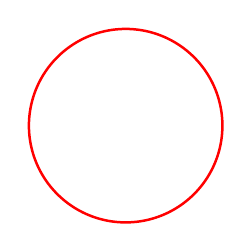
\begin{tikzpicture}[scale=0.45]

  \begin{axis}[
    hide axis,
    axis equal image,
    xmin = -1.42,
    xmax = 1.42,
    ymin = -1.42,
    ymax = 1.42,
    xtick = \empty,
    ytick = \empty,
    title style={align=left},
%    title={\Large $t = 1.00 \times 10^{0}$ \\ \\ \Large $\nu = 1.00$}
  ]

\addplot[red,line width=2pt] coordinates{
(1.3619e+00,-2.0922e-10)
(1.3616e+00,2.7822e-02)
(1.3608e+00,5.6341e-02)
(1.3592e+00,8.6156e-02)
(1.3568e+00,1.1771e-01)
(1.3535e+00,1.5125e-01)
(1.3490e+00,1.8685e-01)
(1.3433e+00,2.2444e-01)
(1.3361e+00,2.6377e-01)
(1.3274e+00,3.0454e-01)
(1.3172e+00,3.4632e-01)
(1.3053e+00,3.8864e-01)
(1.2919e+00,4.3100e-01)
(1.2772e+00,4.7288e-01)
(1.2613e+00,5.1374e-01)
(1.2446e+00,5.5311e-01)
(1.2273e+00,5.9051e-01)
(1.2098e+00,6.2553e-01)
(1.1925e+00,6.5782e-01)
(1.1759e+00,6.8709e-01)
(1.1603e+00,7.1312e-01)
(1.1461e+00,7.3578e-01)
(1.1335e+00,7.5504e-01)
(1.1227e+00,7.7100e-01)
(1.1137e+00,7.8398e-01)
(1.1060e+00,7.9469e-01)
(1.0990e+00,8.0438e-01)
(1.0914e+00,8.1464e-01)
(1.0823e+00,8.2676e-01)
(1.0709e+00,8.4142e-01)
(1.0570e+00,8.5881e-01)
(1.0404e+00,8.7884e-01)
(1.0210e+00,9.0128e-01)
(9.9889e-01,9.2577e-01)
(9.7404e-01,9.5189e-01)
(9.4662e-01,9.7916e-01)
(9.1684e-01,1.0071e+00)
(8.8497e-01,1.0352e+00)
(8.5132e-01,1.0631e+00)
(8.1628e-01,1.0902e+00)
(7.8026e-01,1.1163e+00)
(7.4372e-01,1.1409e+00)
(7.0712e-01,1.1640e+00)
(6.7091e-01,1.1852e+00)
(6.3551e-01,1.2046e+00)
(6.0127e-01,1.2220e+00)
(5.6847e-01,1.2376e+00)
(5.3727e-01,1.2515e+00)
(5.0769e-01,1.2638e+00)
(4.7956e-01,1.2747e+00)
(4.5254e-01,1.2845e+00)
(4.2613e-01,1.2935e+00)
(3.9967e-01,1.3020e+00)
(3.7249e-01,1.3100e+00)
(3.4398e-01,1.3178e+00)
(3.1365e-01,1.3253e+00)
(2.8118e-01,1.3326e+00)
(2.4640e-01,1.3395e+00)
(2.0933e-01,1.3457e+00)
(1.7011e-01,1.3513e+00)
(1.2899e-01,1.3558e+00)
(8.6333e-02,1.3592e+00)
(4.2577e-02,1.3613e+00)
(-1.7828e-03,1.3619e+00)
(-4.6212e-02,1.3611e+00)
(-9.0152e-02,1.3589e+00)
(-1.3305e-01,1.3554e+00)
(-1.7434e-01,1.3507e+00)
(-2.1353e-01,1.3451e+00)
(-2.5014e-01,1.3388e+00)
(-2.8375e-01,1.3320e+00)
(-3.1403e-01,1.3252e+00)
(-3.4072e-01,1.3186e+00)
(-3.6368e-01,1.3125e+00)
(-3.8292e-01,1.3070e+00)
(-3.9868e-01,1.3023e+00)
(-4.1165e-01,1.2982e+00)
(-4.2312e-01,1.2945e+00)
(-4.3494e-01,1.2906e+00)
(-4.4876e-01,1.2859e+00)
(-4.6555e-01,1.2799e+00)
(-4.8570e-01,1.2724e+00)
(-5.0922e-01,1.2631e+00)
(-5.3595e-01,1.2520e+00)
(-5.6556e-01,1.2389e+00)
(-5.9763e-01,1.2238e+00)
(-6.3170e-01,1.2066e+00)
(-6.6725e-01,1.1873e+00)
(-7.0372e-01,1.1660e+00)
(-7.4059e-01,1.1430e+00)
(-7.7731e-01,1.1183e+00)
(-8.1341e-01,1.0923e+00)
(-8.4843e-01,1.0654e+00)
(-8.8198e-01,1.0378e+00)
(-9.1376e-01,1.0099e+00)
(-9.4353e-01,9.8214e-01)
(-9.7114e-01,9.5484e-01)
(-9.9655e-01,9.2829e-01)
(-1.0198e+00,9.0270e-01)
(-1.0410e+00,8.7815e-01)
(-1.0604e+00,8.5460e-01)
(-1.0784e+00,8.3183e-01)
(-1.0953e+00,8.0946e-01)
(-1.1115e+00,7.8699e-01)
(-1.1276e+00,7.6384e-01)
(-1.1437e+00,7.3944e-01)
(-1.1602e+00,7.1331e-01)
(-1.1771e+00,6.8512e-01)
(-1.1943e+00,6.5464e-01)
(-1.2117e+00,6.2179e-01)
(-1.2291e+00,5.8664e-01)
(-1.2462e+00,5.4934e-01)
(-1.2628e+00,5.1015e-01)
(-1.2785e+00,4.6944e-01)
(-1.2931e+00,4.2762e-01)
(-1.3063e+00,3.8518e-01)
(-1.3181e+00,3.4266e-01)
(-1.3283e+00,3.0061e-01)
(-1.3370e+00,2.5961e-01)
(-1.3440e+00,2.2021e-01)
(-1.3496e+00,1.8295e-01)
(-1.3538e+00,1.4833e-01)
(-1.3569e+00,1.1677e-01)
(-1.3590e+00,8.8624e-02)
(-1.3604e+00,6.4142e-02)
(-1.3612e+00,4.3410e-02)
(-1.3617e+00,2.6284e-02)
(-1.3619e+00,1.2214e-02)
(-1.3619e+00,2.2277e-10)
(-1.3619e+00,-1.2214e-02)
(-1.3617e+00,-2.6284e-02)
(-1.3612e+00,-4.3410e-02)
(-1.3604e+00,-6.4142e-02)
(-1.3590e+00,-8.8624e-02)
(-1.3569e+00,-1.1677e-01)
(-1.3538e+00,-1.4833e-01)
(-1.3496e+00,-1.8295e-01)
(-1.3440e+00,-2.2021e-01)
(-1.3370e+00,-2.5961e-01)
(-1.3283e+00,-3.0061e-01)
(-1.3181e+00,-3.4266e-01)
(-1.3063e+00,-3.8518e-01)
(-1.2931e+00,-4.2762e-01)
(-1.2785e+00,-4.6944e-01)
(-1.2628e+00,-5.1015e-01)
(-1.2462e+00,-5.4934e-01)
(-1.2291e+00,-5.8664e-01)
(-1.2117e+00,-6.2179e-01)
(-1.1943e+00,-6.5464e-01)
(-1.1771e+00,-6.8512e-01)
(-1.1602e+00,-7.1331e-01)
(-1.1437e+00,-7.3944e-01)
(-1.1276e+00,-7.6384e-01)
(-1.1115e+00,-7.8699e-01)
(-1.0953e+00,-8.0946e-01)
(-1.0784e+00,-8.3183e-01)
(-1.0604e+00,-8.5460e-01)
(-1.0410e+00,-8.7815e-01)
(-1.0198e+00,-9.0270e-01)
(-9.9655e-01,-9.2829e-01)
(-9.7114e-01,-9.5484e-01)
(-9.4353e-01,-9.8214e-01)
(-9.1376e-01,-1.0099e+00)
(-8.8198e-01,-1.0378e+00)
(-8.4843e-01,-1.0654e+00)
(-8.1341e-01,-1.0923e+00)
(-7.7731e-01,-1.1183e+00)
(-7.4059e-01,-1.1430e+00)
(-7.0372e-01,-1.1660e+00)
(-6.6725e-01,-1.1873e+00)
(-6.3170e-01,-1.2066e+00)
(-5.9763e-01,-1.2238e+00)
(-5.6556e-01,-1.2389e+00)
(-5.3595e-01,-1.2520e+00)
(-5.0922e-01,-1.2631e+00)
(-4.8570e-01,-1.2724e+00)
(-4.6555e-01,-1.2799e+00)
(-4.4876e-01,-1.2859e+00)
(-4.3494e-01,-1.2906e+00)
(-4.2312e-01,-1.2945e+00)
(-4.1165e-01,-1.2982e+00)
(-3.9868e-01,-1.3023e+00)
(-3.8292e-01,-1.3070e+00)
(-3.6368e-01,-1.3125e+00)
(-3.4072e-01,-1.3186e+00)
(-3.1403e-01,-1.3252e+00)
(-2.8375e-01,-1.3320e+00)
(-2.5014e-01,-1.3388e+00)
(-2.1353e-01,-1.3451e+00)
(-1.7434e-01,-1.3507e+00)
(-1.3305e-01,-1.3554e+00)
(-9.0152e-02,-1.3589e+00)
(-4.6212e-02,-1.3611e+00)
(-1.7828e-03,-1.3619e+00)
(4.2577e-02,-1.3613e+00)
(8.6333e-02,-1.3592e+00)
(1.2899e-01,-1.3558e+00)
(1.7011e-01,-1.3513e+00)
(2.0933e-01,-1.3457e+00)
(2.4640e-01,-1.3395e+00)
(2.8118e-01,-1.3326e+00)
(3.1365e-01,-1.3253e+00)
(3.4398e-01,-1.3178e+00)
(3.7249e-01,-1.3100e+00)
(3.9967e-01,-1.3020e+00)
(4.2613e-01,-1.2935e+00)
(4.5254e-01,-1.2845e+00)
(4.7956e-01,-1.2747e+00)
(5.0769e-01,-1.2638e+00)
(5.3727e-01,-1.2515e+00)
(5.6847e-01,-1.2376e+00)
(6.0127e-01,-1.2220e+00)
(6.3551e-01,-1.2046e+00)
(6.7091e-01,-1.1852e+00)
(7.0712e-01,-1.1640e+00)
(7.4372e-01,-1.1409e+00)
(7.8026e-01,-1.1163e+00)
(8.1628e-01,-1.0902e+00)
(8.5132e-01,-1.0631e+00)
(8.8497e-01,-1.0352e+00)
(9.1684e-01,-1.0071e+00)
(9.4662e-01,-9.7916e-01)
(9.7404e-01,-9.5189e-01)
(9.9889e-01,-9.2577e-01)
(1.0210e+00,-9.0128e-01)
(1.0404e+00,-8.7884e-01)
(1.0570e+00,-8.5881e-01)
(1.0709e+00,-8.4142e-01)
(1.0823e+00,-8.2676e-01)
(1.0914e+00,-8.1464e-01)
(1.0990e+00,-8.0438e-01)
(1.1060e+00,-7.9469e-01)
(1.1137e+00,-7.8398e-01)
(1.1227e+00,-7.7100e-01)
(1.1335e+00,-7.5504e-01)
(1.1461e+00,-7.3578e-01)
(1.1603e+00,-7.1312e-01)
(1.1759e+00,-6.8709e-01)
(1.1925e+00,-6.5782e-01)
(1.2098e+00,-6.2553e-01)
(1.2273e+00,-5.9051e-01)
(1.2446e+00,-5.5311e-01)
(1.2613e+00,-5.1374e-01)
(1.2772e+00,-4.7288e-01)
(1.2919e+00,-4.3100e-01)
(1.3053e+00,-3.8864e-01)
(1.3172e+00,-3.4632e-01)
(1.3274e+00,-3.0454e-01)
(1.3361e+00,-2.6377e-01)
(1.3433e+00,-2.2444e-01)
(1.3490e+00,-1.8685e-01)
(1.3535e+00,-1.5125e-01)
(1.3568e+00,-1.1771e-01)
(1.3592e+00,-8.6156e-02)
(1.3608e+00,-5.6341e-02)
(1.3616e+00,-2.7822e-02)
(1.3619e+00,-2.0922e-10)
};



\end{axis}

\end{tikzpicture}

%%    \fi
%  \end{minipage}
%  \hfill
%  \begin{minipage}{0.4\textwidth}
%%  \ifTikz
%  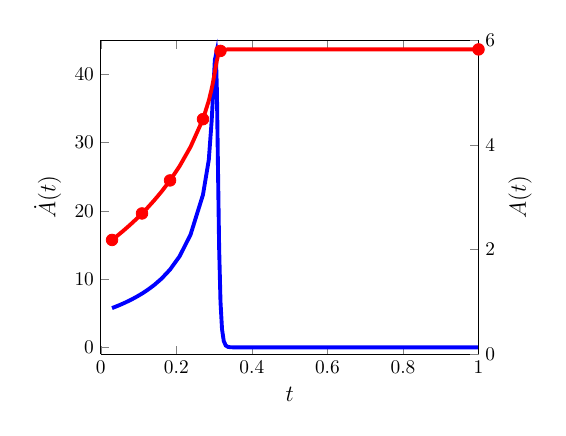
\begin{tikzpicture}[scale=0.7]

  \begin{axis}[
    label = area,
    axis y line*=left,
    xmin = 0,
    xmax = 1,
    ymin = -1,
    ymax = 45,
%    xtick = \empty,
%    ytick = \empty,
    xlabel = {\large $t$},
    ylabel = {\large $\dot{A}(t)$},
    ylabel near ticks,
    clip = false,
  ]

\addplot[blue, line width=2pt] coordinates{
(2.9870e-02,5.7561e+00)
(3.4004e-02,5.8445e+00)
(3.8711e-02,5.9473e+00)
(4.4069e-02,6.0675e+00)
(5.0169e-02,6.2087e+00)
(5.7113e-02,6.3756e+00)
(6.5018e-02,6.5740e+00)
(7.4018e-02,6.8114e+00)
(8.4263e-02,7.0984e+00)
(9.5927e-02,7.4491e+00)
(1.0920e-01,7.8837e+00)
(1.2432e-01,8.4323e+00)
(1.4153e-01,9.1412e+00)
(1.6112e-01,1.0086e+01)
(1.8342e-01,1.1403e+01)
(2.0881e-01,1.3355e+01)
(2.3771e-01,1.6528e+01)
(2.7062e-01,2.2375e+01)
(2.8600e-01,2.7491e+01)
(2.9355e-01,3.3172e+01)
(2.9843e-01,3.8204e+01)
(3.0194e-01,4.2097e+01)
(3.0477e-01,4.2847e+01)
(3.0746e-01,3.7637e+01)
(3.1022e-01,2.6545e+01)
(3.1336e-01,1.4603e+01)
(3.1693e-01,6.7105e+00)
(3.2099e-01,2.6631e+00)
(3.2562e-01,9.1879e-01)
(3.3089e-01,2.7242e-01)
(3.3689e-01,6.8267e-02)
(3.4372e-01,1.4117e-02)
(3.5149e-01,2.3475e-03)
(3.6034e-01,3.0278e-04)
(3.7042e-01,2.9334e-05)
(3.8189e-01,1.8397e-06)
(3.9495e-01,2.9182e-08)
(4.0981e-01,-1.1297e-07)
(4.2673e-01,-8.9110e-08)
(4.4600e-01,-1.0247e-07)
(4.6793e-01,-9.5801e-08)
(4.9290e-01,-9.8909e-08)
(5.2132e-01,-9.7487e-08)
(5.5368e-01,-9.8115e-08)
(5.9052e-01,-9.7979e-08)
(6.3245e-01,-9.8076e-08)
(6.8019e-01,-9.8003e-08)
(7.3454e-01,-9.7982e-08)
(7.9642e-01,-9.8078e-08)
(8.6685e-01,-9.7981e-08)
(9.4704e-01,-9.8083e-08)
(1.0000e+00,-9.7890e-08)
};

%\node at (axis cs:0,45) [anchor=south east] {(a)};

\end{axis}

  \begin{axis}[
    axis y line*=right,
    axis x line=none,
    xmin = 0,
    xmax = 1,
    ymin = 0,
    ymax = 6,
%    xtick = \empty,
%    ytick = \empty,
    ylabel = {\large $A(t)$},
    ylabel near ticks,
  ]


\addplot[red,line width=2pt] coordinates{
(2.9870e-02,2.1842e+00)
(3.4004e-02,2.2076e+00)
(3.8711e-02,2.2346e+00)
(4.4069e-02,2.2658e+00)
(5.0169e-02,2.3019e+00)
(5.7113e-02,2.3438e+00)
(6.5018e-02,2.3927e+00)
(7.4018e-02,2.4498e+00)
(8.4263e-02,2.5170e+00)
(9.5927e-02,2.5963e+00)
(1.0920e-01,2.6907e+00)
(1.2432e-01,2.8039e+00)
(1.4153e-01,2.9413e+00)
(1.6112e-01,3.1103e+00)
(1.8342e-01,3.3225e+00)
(2.0881e-01,3.5962e+00)
(2.3771e-01,3.9645e+00)
(2.7062e-01,4.4934e+00)
(2.8600e-01,4.8471e+00)
(2.9355e-01,5.0730e+00)
(2.9843e-01,5.2478e+00)
(3.0194e-01,5.3903e+00)
(3.0477e-01,5.5117e+00)
(3.0746e-01,5.6188e+00)
(3.1022e-01,5.7036e+00)
(3.1336e-01,5.7637e+00)
(3.1693e-01,5.7985e+00)
(3.2099e-01,5.8158e+00)
(3.2562e-01,5.8232e+00)
(3.3089e-01,5.8260e+00)
(3.3689e-01,5.8269e+00)
(3.4372e-01,5.8271e+00)
(3.5149e-01,5.8272e+00)
(3.6034e-01,5.8272e+00)
(3.7042e-01,5.8272e+00)
(3.8189e-01,5.8272e+00)
(3.9495e-01,5.8272e+00)
(4.0981e-01,5.8272e+00)
(4.2673e-01,5.8272e+00)
(4.4600e-01,5.8272e+00)
(4.6793e-01,5.8272e+00)
(4.9290e-01,5.8272e+00)
(5.2132e-01,5.8272e+00)
(5.5368e-01,5.8272e+00)
(5.9052e-01,5.8272e+00)
(6.3245e-01,5.8272e+00)
(6.8019e-01,5.8272e+00)
(7.3454e-01,5.8272e+00)
(7.9642e-01,5.8272e+00)
(8.6685e-01,5.8272e+00)
(9.4704e-01,5.8272e+00)
(1.0000e+00,5.8272e+00)
};

\addplot[red,only marks,mark size=3pt] coordinates{
(2.9870e-02,2.1842e+00)
(1.0920e-01,2.6907e+00)
(1.8342e-01,3.3225e+00)
(2.7062e-01,4.4934e+00)
(3.1693e-01,5.7985e+00)
(1.0000e+00,5.8272e+00)
};



\end{axis}



\end{tikzpicture}

%%  \fi
%  \end{minipage}
%%  \caption{\label{fig:starShape} A initially star-shaped semi-permeable
%%  vesicle in a shear quiescent flow with $\beta=1$. Note that the time
%%  steps are not equispaced. The area (red) and its derivative (blue) of
%%  an initially star-shaped vesicle as a function of time. The dots
%%  correspond to the time steps shown in six time steps
%%  show on the left.}
%\end{figure}
%
%\begin{table}[htp]
%  \centering
%  \begin{tabular}{|C{1cm}|*{6}{C{2cm}}|}
%    \hline
%    $\beta$ & $10^{0}$ & $10^{-1}$ & $10^{-2}$ & 
%             $10^{-3}$ & $10^{-4}$ & $10^{-5}$ \\
%    $t_\mathrm{SS}$ & $6.45 \times 10^{0}$ & $2.00 \times 10^{1}$ & 
%                      $9.61 \times 10^{1}$ & $8.36 \times 10^{2}$ & 
%                      $8.15 \times 10^{3}$ & $8.03 \times 10^{4}$ \\
%    ratio & --- & 3.10 & 4.81 & 8.71 & 9.74 & 9.85 \\
%    \hline
%  \end{tabular}
%  \caption{\label{tbl:ellipseRelaxTime} The time, $t_{\mathrm{SS}}$, for
%  a semi-permeable vesicle to reach steady state.}
%\end{table}
%
%\begin{table}[htp]
%  \centering
%  \begin{tabular}{|C{1cm}|*{6}{C{2cm}}|}
%    \hline
%    $\beta$ & $10^{0}$ & $10^{-1}$ & $10^{-2}$ & 
%             $10^{-3}$ & $10^{-4}$ & $10^{-5}$ \\
%    $t_\mathrm{SP}$ & $2.17 \times 10^{-2}$ & $1.25 \times 10^{-1}$ & 
%                      $1.59 \times 10^{0}$ & $2.19 \times 10^{1}$ & 
%                      $2.14 \times 10^{2}$ & $2.20 \times 10^{3}$ \\
%    ratio & --- & 5.76 & 12.72 & 13.77 & 9.77 & 10.14 \\
%    \hline
%  \end{tabular}
%  \caption{\label{tbl:ellipseBLTime} The time, $t_\mathrm{SP}$, for a
%  semi-permeable vesicle to begin inflating.}
%\end{table}
%
%%\begin{figure}[htp]
%%\begin{minipage}{0.40\textwidth}
%%\ifTikz
%%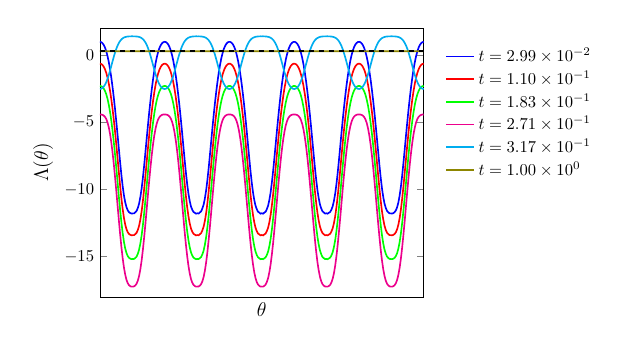
\begin{tikzpicture}[scale=0.6]

  \begin{axis}[
    xmin = 0,
    xmax = 6.2832,
    ymin = -18,
    ymax = 2,
    xtick = \empty,
    ylabel near ticks,
    xlabel = {\large $\theta$},
    ylabel = {\large $\Lambda(\theta)$},
    clip = false,
    legend entries = {$t=2.99 \times 10^{-2}$,
    $t = 1.10 \times 10^{-1}$,
    $t = 1.83 \times 10^{-1}$,
    $t = 2.71 \times 10^{-1}$,
    $t = 3.17 \times 10^{-1}$,
    $t = 1.00 \times 10^{0}$},
    legend cell align=left,
    legend style={draw=none},
    legend style={at={(1.05,0.95)},anchor=north west}
  ]


\addplot[blue,line width=1pt] coordinates{
(0.0000e+00,9.7332e-01)
(2.4544e-02,9.5053e-01)
(4.9087e-02,8.7407e-01)
(7.3631e-02,7.4345e-01)
(9.8175e-02,5.4519e-01)
(1.2272e-01,2.7392e-01)
(1.4726e-01,-8.1963e-02)
(1.7181e-01,-5.2587e-01)
(1.9635e-01,-1.0619e+00)
(2.2089e-01,-1.6879e+00)
(2.4544e-01,-2.4009e+00)
(2.6998e-01,-3.1957e+00)
(2.9452e-01,-4.0665e+00)
(3.1907e-01,-5.0048e+00)
(3.4361e-01,-5.9949e+00)
(3.6816e-01,-7.0104e+00)
(3.9270e-01,-8.0105e+00)
(4.1724e-01,-8.9464e+00)
(4.4179e-01,-9.7689e+00)
(4.6633e-01,-1.0445e+01)
(4.9087e-01,-1.0959e+01)
(5.1542e-01,-1.1322e+01)
(5.3996e-01,-1.1556e+01)
(5.6450e-01,-1.1694e+01)
(5.8905e-01,-1.1761e+01)
(6.1359e-01,-1.1796e+01)
(6.3814e-01,-1.1785e+01)
(6.6268e-01,-1.1781e+01)
(6.8722e-01,-1.1703e+01)
(7.1177e-01,-1.1598e+01)
(7.3631e-01,-1.1373e+01)
(7.6085e-01,-1.1048e+01)
(7.8540e-01,-1.0556e+01)
(8.0994e-01,-9.9198e+00)
(8.3449e-01,-9.1187e+00)
(8.5903e-01,-8.2065e+00)
(8.8357e-01,-7.2117e+00)
(9.0812e-01,-6.1982e+00)
(9.3266e-01,-5.1986e+00)
(9.5720e-01,-4.2496e+00)
(9.8175e-01,-3.3638e+00)
(1.0063e+00,-2.5535e+00)
(1.0308e+00,-1.8239e+00)
(1.0554e+00,-1.1796e+00)
(1.0799e+00,-6.2629e-01)
(1.1045e+00,-1.6283e-01)
(1.1290e+00,2.0889e-01)
(1.1536e+00,4.9796e-01)
(1.1781e+00,7.0867e-01)
(1.2026e+00,8.5323e-01)
(1.2272e+00,9.3921e-01)
(1.2517e+00,9.7257e-01)
(1.2763e+00,9.5943e-01)
(1.3008e+00,8.9299e-01)
(1.3254e+00,7.7536e-01)
(1.3499e+00,5.8960e-01)
(1.3744e+00,3.3549e-01)
(1.3990e+00,-4.6191e-03)
(1.4235e+00,-4.2912e-01)
(1.4481e+00,-9.4790e-01)
(1.4726e+00,-1.5553e+00)
(1.4972e+00,-2.2517e+00)
(1.5217e+00,-3.0306e+00)
(1.5463e+00,-3.8863e+00)
(1.5708e+00,-4.8130e+00)
(1.5953e+00,-5.7928e+00)
(1.6199e+00,-6.8084e+00)
(1.6444e+00,-7.8122e+00)
(1.6690e+00,-8.7692e+00)
(1.6935e+00,-9.6124e+00)
(1.7181e+00,-1.0326e+01)
(1.7426e+00,-1.0865e+01)
(1.7671e+00,-1.1267e+01)
(1.7917e+00,-1.1512e+01)
(1.8162e+00,-1.1681e+01)
(1.8408e+00,-1.1741e+01)
(1.8653e+00,-1.1804e+01)
(1.8899e+00,-1.1776e+01)
(1.9144e+00,-1.1797e+01)
(1.9390e+00,-1.1712e+01)
(1.9635e+00,-1.1634e+01)
(1.9880e+00,-1.1420e+01)
(2.0126e+00,-1.1130e+01)
(2.0371e+00,-1.0663e+01)
(2.0617e+00,-1.0064e+01)
(2.0862e+00,-9.2869e+00)
(2.1108e+00,-8.3989e+00)
(2.1353e+00,-7.4123e+00)
(2.1598e+00,-6.4020e+00)
(2.1844e+00,-5.3945e+00)
(2.2089e+00,-4.4353e+00)
(2.2335e+00,-3.5349e+00)
(2.2580e+00,-2.7094e+00)
(2.2826e+00,-1.9632e+00)
(2.3071e+00,-1.3010e+00)
(2.3317e+00,-7.3017e-01)
(2.3562e+00,-2.4753e-01)
(2.3807e+00,1.4070e-01)
(2.4053e+00,4.4747e-01)
(2.4298e+00,6.7129e-01)
(2.4544e+00,8.3009e-01)
(2.4789e+00,9.2567e-01)
(2.5035e+00,9.7019e-01)
(2.5280e+00,9.6592e-01)
(2.5525e+00,9.1019e-01)
(2.5771e+00,8.0422e-01)
(2.6016e+00,6.3158e-01)
(2.6262e+00,3.9337e-01)
(2.6507e+00,6.9535e-02)
(2.6753e+00,-3.3629e-01)
(2.6998e+00,-8.3736e-01)
(2.7243e+00,-1.4263e+00)
(2.7489e+00,-2.1058e+00)
(2.7734e+00,-2.8684e+00)
(2.7980e+00,-3.7090e+00)
(2.8225e+00,-4.6232e+00)
(2.8471e+00,-5.5926e+00)
(2.8716e+00,-6.6055e+00)
(2.8962e+00,-7.6126e+00)
(2.9207e+00,-8.5866e+00)
(2.9452e+00,-9.4515e+00)
(2.9698e+00,-1.0199e+01)
(2.9943e+00,-1.0766e+01)
(3.0189e+00,-1.1203e+01)
(3.0434e+00,-1.1466e+01)
(3.0680e+00,-1.1661e+01)
(3.0925e+00,-1.1724e+01)
(3.1170e+00,-1.1805e+01)
(3.1416e+00,-1.1772e+01)
(3.1661e+00,-1.1805e+01)
(3.1907e+00,-1.1724e+01)
(3.2152e+00,-1.1661e+01)
(3.2398e+00,-1.1466e+01)
(3.2643e+00,-1.1203e+01)
(3.2889e+00,-1.0766e+01)
(3.3134e+00,-1.0199e+01)
(3.3379e+00,-9.4515e+00)
(3.3625e+00,-8.5866e+00)
(3.3870e+00,-7.6126e+00)
(3.4116e+00,-6.6055e+00)
(3.4361e+00,-5.5926e+00)
(3.4607e+00,-4.6232e+00)
(3.4852e+00,-3.7090e+00)
(3.5097e+00,-2.8684e+00)
(3.5343e+00,-2.1058e+00)
(3.5588e+00,-1.4263e+00)
(3.5834e+00,-8.3736e-01)
(3.6079e+00,-3.3629e-01)
(3.6325e+00,6.9535e-02)
(3.6570e+00,3.9337e-01)
(3.6816e+00,6.3158e-01)
(3.7061e+00,8.0422e-01)
(3.7306e+00,9.1019e-01)
(3.7552e+00,9.6592e-01)
(3.7797e+00,9.7019e-01)
(3.8043e+00,9.2567e-01)
(3.8288e+00,8.3009e-01)
(3.8534e+00,6.7129e-01)
(3.8779e+00,4.4747e-01)
(3.9024e+00,1.4070e-01)
(3.9270e+00,-2.4753e-01)
(3.9515e+00,-7.3017e-01)
(3.9761e+00,-1.3010e+00)
(4.0006e+00,-1.9632e+00)
(4.0252e+00,-2.7094e+00)
(4.0497e+00,-3.5349e+00)
(4.0743e+00,-4.4353e+00)
(4.0988e+00,-5.3945e+00)
(4.1233e+00,-6.4020e+00)
(4.1479e+00,-7.4123e+00)
(4.1724e+00,-8.3989e+00)
(4.1970e+00,-9.2869e+00)
(4.2215e+00,-1.0064e+01)
(4.2461e+00,-1.0663e+01)
(4.2706e+00,-1.1130e+01)
(4.2951e+00,-1.1420e+01)
(4.3197e+00,-1.1634e+01)
(4.3442e+00,-1.1712e+01)
(4.3688e+00,-1.1797e+01)
(4.3933e+00,-1.1776e+01)
(4.4179e+00,-1.1804e+01)
(4.4424e+00,-1.1741e+01)
(4.4670e+00,-1.1681e+01)
(4.4915e+00,-1.1512e+01)
(4.5160e+00,-1.1267e+01)
(4.5406e+00,-1.0865e+01)
(4.5651e+00,-1.0326e+01)
(4.5897e+00,-9.6124e+00)
(4.6142e+00,-8.7692e+00)
(4.6388e+00,-7.8122e+00)
(4.6633e+00,-6.8084e+00)
(4.6878e+00,-5.7928e+00)
(4.7124e+00,-4.8130e+00)
(4.7369e+00,-3.8863e+00)
(4.7615e+00,-3.0306e+00)
(4.7860e+00,-2.2517e+00)
(4.8106e+00,-1.5553e+00)
(4.8351e+00,-9.4790e-01)
(4.8597e+00,-4.2912e-01)
(4.8842e+00,-4.6191e-03)
(4.9087e+00,3.3549e-01)
(4.9333e+00,5.8960e-01)
(4.9578e+00,7.7536e-01)
(4.9824e+00,8.9299e-01)
(5.0069e+00,9.5943e-01)
(5.0315e+00,9.7257e-01)
(5.0560e+00,9.3921e-01)
(5.0805e+00,8.5323e-01)
(5.1051e+00,7.0867e-01)
(5.1296e+00,4.9796e-01)
(5.1542e+00,2.0889e-01)
(5.1787e+00,-1.6283e-01)
(5.2033e+00,-6.2629e-01)
(5.2278e+00,-1.1796e+00)
(5.2524e+00,-1.8239e+00)
(5.2769e+00,-2.5535e+00)
(5.3014e+00,-3.3638e+00)
(5.3260e+00,-4.2496e+00)
(5.3505e+00,-5.1986e+00)
(5.3751e+00,-6.1982e+00)
(5.3996e+00,-7.2117e+00)
(5.4242e+00,-8.2065e+00)
(5.4487e+00,-9.1187e+00)
(5.4732e+00,-9.9198e+00)
(5.4978e+00,-1.0556e+01)
(5.5223e+00,-1.1048e+01)
(5.5469e+00,-1.1373e+01)
(5.5714e+00,-1.1598e+01)
(5.5960e+00,-1.1703e+01)
(5.6205e+00,-1.1781e+01)
(5.6450e+00,-1.1785e+01)
(5.6696e+00,-1.1796e+01)
(5.6941e+00,-1.1761e+01)
(5.7187e+00,-1.1694e+01)
(5.7432e+00,-1.1556e+01)
(5.7678e+00,-1.1322e+01)
(5.7923e+00,-1.0959e+01)
(5.8169e+00,-1.0445e+01)
(5.8414e+00,-9.7689e+00)
(5.8659e+00,-8.9464e+00)
(5.8905e+00,-8.0105e+00)
(5.9150e+00,-7.0104e+00)
(5.9396e+00,-5.9949e+00)
(5.9641e+00,-5.0048e+00)
(5.9887e+00,-4.0665e+00)
(6.0132e+00,-3.1957e+00)
(6.0377e+00,-2.4009e+00)
(6.0623e+00,-1.6879e+00)
(6.0868e+00,-1.0619e+00)
(6.1114e+00,-5.2587e-01)
(6.1359e+00,-8.1963e-02)
(6.1605e+00,2.7392e-01)
(6.1850e+00,5.4519e-01)
(6.2096e+00,7.4345e-01)
(6.2341e+00,8.7407e-01)
(6.2586e+00,9.5053e-01)
(6.2832e+00,9.7332e-01)
};

\addplot[red,line width=1pt] coordinates{
(0.0000e+00,-6.5079e-01)
(2.4544e-02,-6.7293e-01)
(4.9087e-02,-7.4659e-01)
(7.3631e-02,-8.7322e-01)
(9.8175e-02,-1.0660e+00)
(1.2272e-01,-1.3316e+00)
(1.4726e-01,-1.6823e+00)
(1.7181e-01,-2.1235e+00)
(1.9635e-01,-2.6612e+00)
(2.2089e-01,-3.2953e+00)
(2.4544e-01,-4.0249e+00)
(2.6998e-01,-4.8447e+00)
(2.9452e-01,-5.7468e+00)
(3.1907e-01,-6.7172e+00)
(3.4361e-01,-7.7329e+00)
(3.6816e-01,-8.7606e+00)
(3.9270e-01,-9.7566e+00)
(4.1724e-01,-1.0674e+01)
(4.4179e-01,-1.1471e+01)
(4.6633e-01,-1.2120e+01)
(4.9087e-01,-1.2613e+01)
(5.1542e-01,-1.2960e+01)
(5.3996e-01,-1.3183e+01)
(5.6450e-01,-1.3314e+01)
(5.8905e-01,-1.3379e+01)
(6.1359e-01,-1.3411e+01)
(6.3814e-01,-1.3402e+01)
(6.6268e-01,-1.3396e+01)
(6.8722e-01,-1.3324e+01)
(7.1177e-01,-1.3222e+01)
(7.3631e-01,-1.3008e+01)
(7.6085e-01,-1.2697e+01)
(7.8540e-01,-1.2228e+01)
(8.0994e-01,-1.1616e+01)
(8.3449e-01,-1.0842e+01)
(8.5903e-01,-9.9495e+00)
(8.8357e-01,-8.9626e+00)
(9.0812e-01,-7.9396e+00)
(9.3266e-01,-6.9170e+00)
(9.5720e-01,-5.9364e+00)
(9.8175e-01,-5.0188e+00)
(1.0063e+00,-4.1817e+00)
(1.0308e+00,-3.4339e+00)
(1.0554e+00,-2.7799e+00)
(1.0799e+00,-2.2238e+00)
(1.1045e+00,-1.7625e+00)
(1.1290e+00,-1.3954e+00)
(1.1536e+00,-1.1123e+00)
(1.1781e+00,-9.0686e-01)
(1.2026e+00,-7.6685e-01)
(1.2272e+00,-6.8376e-01)
(1.2517e+00,-6.5155e-01)
(1.2763e+00,-6.6437e-01)
(1.3008e+00,-7.2824e-01)
(1.3254e+00,-8.4238e-01)
(1.3499e+00,-1.0226e+00)
(1.3744e+00,-1.2713e+00)
(1.3990e+00,-1.6058e+00)
(1.4235e+00,-2.0271e+00)
(1.4481e+00,-2.5464e+00)
(1.4726e+00,-3.1605e+00)
(1.4972e+00,-3.8717e+00)
(1.5217e+00,-4.6739e+00)
(1.5463e+00,-5.5601e+00)
(1.5708e+00,-6.5191e+00)
(1.5953e+00,-7.5268e+00)
(1.6199e+00,-8.5572e+00)
(1.6444e+00,-9.5607e+00)
(1.6690e+00,-1.0501e+01)
(1.6935e+00,-1.1321e+01)
(1.7181e+00,-1.2006e+01)
(1.7426e+00,-1.2523e+01)
(1.7671e+00,-1.2906e+01)
(1.7917e+00,-1.3141e+01)
(1.8162e+00,-1.3301e+01)
(1.8408e+00,-1.3361e+01)
(1.8653e+00,-1.3418e+01)
(1.8899e+00,-1.3395e+01)
(1.9144e+00,-1.3410e+01)
(1.9390e+00,-1.3334e+01)
(1.9635e+00,-1.3255e+01)
(1.9880e+00,-1.3054e+01)
(2.0126e+00,-1.2775e+01)
(2.0371e+00,-1.2331e+01)
(2.0617e+00,-1.1754e+01)
(2.0862e+00,-1.1006e+01)
(2.1108e+00,-1.0138e+01)
(2.1353e+00,-9.1633e+00)
(2.1598e+00,-8.1463e+00)
(2.1844e+00,-7.1186e+00)
(2.2089e+00,-6.1285e+00)
(2.2335e+00,-5.1961e+00)
(2.2580e+00,-4.3423e+00)
(2.2826e+00,-3.5762e+00)
(2.3071e+00,-2.9027e+00)
(2.3317e+00,-2.3278e+00)
(2.3562e+00,-1.8466e+00)
(2.3807e+00,-1.4624e+00)
(2.4053e+00,-1.1617e+00)
(2.4298e+00,-9.4307e-01)
(2.4544e+00,-7.8935e-01)
(2.4789e+00,-6.9674e-01)
(2.5035e+00,-6.5390e-01)
(2.5280e+00,-6.5809e-01)
(2.5525e+00,-7.1162e-01)
(2.5771e+00,-8.1444e-01)
(2.6016e+00,-9.8166e-01)
(2.6262e+00,-1.2146e+00)
(2.6507e+00,-1.5325e+00)
(2.6753e+00,-1.9348e+00)
(2.6998e+00,-2.4353e+00)
(2.7243e+00,-3.0296e+00)
(2.7489e+00,-3.7221e+00)
(2.7734e+00,-4.5064e+00)
(2.7980e+00,-5.3765e+00)
(2.8225e+00,-6.3228e+00)
(2.8471e+00,-7.3219e+00)
(2.8716e+00,-8.3524e+00)
(2.8962e+00,-9.3628e+00)
(2.9207e+00,-1.0323e+01)
(2.9452e+00,-1.1165e+01)
(2.9698e+00,-1.1884e+01)
(2.9943e+00,-1.2429e+01)
(3.0189e+00,-1.2844e+01)
(3.0434e+00,-1.3098e+01)
(3.0680e+00,-1.3281e+01)
(3.0925e+00,-1.3346e+01)
(3.1170e+00,-1.3417e+01)
(3.1416e+00,-1.3392e+01)
(3.1661e+00,-1.3417e+01)
(3.1907e+00,-1.3346e+01)
(3.2152e+00,-1.3281e+01)
(3.2398e+00,-1.3098e+01)
(3.2643e+00,-1.2844e+01)
(3.2889e+00,-1.2429e+01)
(3.3134e+00,-1.1884e+01)
(3.3379e+00,-1.1165e+01)
(3.3625e+00,-1.0323e+01)
(3.3870e+00,-9.3628e+00)
(3.4116e+00,-8.3524e+00)
(3.4361e+00,-7.3219e+00)
(3.4607e+00,-6.3228e+00)
(3.4852e+00,-5.3765e+00)
(3.5097e+00,-4.5064e+00)
(3.5343e+00,-3.7221e+00)
(3.5588e+00,-3.0296e+00)
(3.5834e+00,-2.4353e+00)
(3.6079e+00,-1.9348e+00)
(3.6325e+00,-1.5325e+00)
(3.6570e+00,-1.2146e+00)
(3.6816e+00,-9.8166e-01)
(3.7061e+00,-8.1444e-01)
(3.7306e+00,-7.1162e-01)
(3.7552e+00,-6.5809e-01)
(3.7797e+00,-6.5390e-01)
(3.8043e+00,-6.9674e-01)
(3.8288e+00,-7.8935e-01)
(3.8534e+00,-9.4307e-01)
(3.8779e+00,-1.1617e+00)
(3.9024e+00,-1.4624e+00)
(3.9270e+00,-1.8466e+00)
(3.9515e+00,-2.3278e+00)
(3.9761e+00,-2.9027e+00)
(4.0006e+00,-3.5762e+00)
(4.0252e+00,-4.3423e+00)
(4.0497e+00,-5.1961e+00)
(4.0743e+00,-6.1285e+00)
(4.0988e+00,-7.1186e+00)
(4.1233e+00,-8.1463e+00)
(4.1479e+00,-9.1633e+00)
(4.1724e+00,-1.0138e+01)
(4.1970e+00,-1.1006e+01)
(4.2215e+00,-1.1754e+01)
(4.2461e+00,-1.2331e+01)
(4.2706e+00,-1.2775e+01)
(4.2951e+00,-1.3054e+01)
(4.3197e+00,-1.3255e+01)
(4.3442e+00,-1.3334e+01)
(4.3688e+00,-1.3410e+01)
(4.3933e+00,-1.3395e+01)
(4.4179e+00,-1.3418e+01)
(4.4424e+00,-1.3361e+01)
(4.4670e+00,-1.3301e+01)
(4.4915e+00,-1.3141e+01)
(4.5160e+00,-1.2906e+01)
(4.5406e+00,-1.2523e+01)
(4.5651e+00,-1.2006e+01)
(4.5897e+00,-1.1321e+01)
(4.6142e+00,-1.0501e+01)
(4.6388e+00,-9.5607e+00)
(4.6633e+00,-8.5572e+00)
(4.6878e+00,-7.5268e+00)
(4.7124e+00,-6.5191e+00)
(4.7369e+00,-5.5601e+00)
(4.7615e+00,-4.6739e+00)
(4.7860e+00,-3.8717e+00)
(4.8106e+00,-3.1605e+00)
(4.8351e+00,-2.5464e+00)
(4.8597e+00,-2.0271e+00)
(4.8842e+00,-1.6058e+00)
(4.9087e+00,-1.2713e+00)
(4.9333e+00,-1.0226e+00)
(4.9578e+00,-8.4238e-01)
(4.9824e+00,-7.2824e-01)
(5.0069e+00,-6.6437e-01)
(5.0315e+00,-6.5155e-01)
(5.0560e+00,-6.8376e-01)
(5.0805e+00,-7.6685e-01)
(5.1051e+00,-9.0686e-01)
(5.1296e+00,-1.1123e+00)
(5.1542e+00,-1.3954e+00)
(5.1787e+00,-1.7625e+00)
(5.2033e+00,-2.2238e+00)
(5.2278e+00,-2.7799e+00)
(5.2524e+00,-3.4339e+00)
(5.2769e+00,-4.1817e+00)
(5.3014e+00,-5.0188e+00)
(5.3260e+00,-5.9364e+00)
(5.3505e+00,-6.9170e+00)
(5.3751e+00,-7.9396e+00)
(5.3996e+00,-8.9626e+00)
(5.4242e+00,-9.9495e+00)
(5.4487e+00,-1.0842e+01)
(5.4732e+00,-1.1616e+01)
(5.4978e+00,-1.2228e+01)
(5.5223e+00,-1.2697e+01)
(5.5469e+00,-1.3008e+01)
(5.5714e+00,-1.3222e+01)
(5.5960e+00,-1.3324e+01)
(5.6205e+00,-1.3396e+01)
(5.6450e+00,-1.3402e+01)
(5.6696e+00,-1.3411e+01)
(5.6941e+00,-1.3379e+01)
(5.7187e+00,-1.3314e+01)
(5.7432e+00,-1.3183e+01)
(5.7678e+00,-1.2960e+01)
(5.7923e+00,-1.2613e+01)
(5.8169e+00,-1.2120e+01)
(5.8414e+00,-1.1471e+01)
(5.8659e+00,-1.0674e+01)
(5.8905e+00,-9.7566e+00)
(5.9150e+00,-8.7606e+00)
(5.9396e+00,-7.7329e+00)
(5.9641e+00,-6.7172e+00)
(5.9887e+00,-5.7468e+00)
(6.0132e+00,-4.8447e+00)
(6.0377e+00,-4.0249e+00)
(6.0623e+00,-3.2953e+00)
(6.0868e+00,-2.6612e+00)
(6.1114e+00,-2.1235e+00)
(6.1359e+00,-1.6823e+00)
(6.1605e+00,-1.3316e+00)
(6.1850e+00,-1.0660e+00)
(6.2096e+00,-8.7322e-01)
(6.2341e+00,-7.4659e-01)
(6.2586e+00,-6.7293e-01)
(6.2832e+00,-6.5079e-01)
};

\addplot[green,line width=1pt] coordinates{
(0.0000e+00,-2.3061e+00)
(2.4544e-02,-2.3254e+00)
(4.9087e-02,-2.3896e+00)
(7.3631e-02,-2.5021e+00)
(9.8175e-02,-2.6769e+00)
(1.2272e-01,-2.9246e+00)
(1.4726e-01,-3.2610e+00)
(1.7181e-01,-3.6958e+00)
(1.9635e-01,-4.2380e+00)
(2.2089e-01,-4.8890e+00)
(2.4544e-01,-5.6470e+00)
(2.6998e-01,-6.5042e+00)
(2.9452e-01,-7.4479e+00)
(3.1907e-01,-8.4580e+00)
(3.4361e-01,-9.5050e+00)
(3.6816e-01,-1.0551e+01)
(3.9270e-01,-1.1553e+01)
(4.1724e-01,-1.2467e+01)
(4.4179e-01,-1.3257e+01)
(4.6633e-01,-1.3899e+01)
(4.9087e-01,-1.4388e+01)
(5.1542e-01,-1.4733e+01)
(5.3996e-01,-1.4956e+01)
(5.6450e-01,-1.5087e+01)
(5.8905e-01,-1.5152e+01)
(6.1359e-01,-1.5184e+01)
(6.3814e-01,-1.5178e+01)
(6.6268e-01,-1.5168e+01)
(6.8722e-01,-1.5099e+01)
(7.1177e-01,-1.4993e+01)
(7.3631e-01,-1.4783e+01)
(7.6085e-01,-1.4471e+01)
(7.8540e-01,-1.4007e+01)
(8.0994e-01,-1.3399e+01)
(8.3449e-01,-1.2634e+01)
(8.5903e-01,-1.1745e+01)
(8.8357e-01,-1.0756e+01)
(9.0812e-01,-9.7163e+00)
(9.3266e-01,-8.6651e+00)
(9.5720e-01,-7.6457e+00)
(9.8175e-01,-6.6865e+00)
(1.0063e+00,-5.8107e+00)
(1.0308e+00,-5.0324e+00)
(1.0554e+00,-4.3591e+00)
(1.0799e+00,-3.7959e+00)
(1.1045e+00,-3.3392e+00)
(1.1290e+00,-2.9849e+00)
(1.1536e+00,-2.7196e+00)
(1.1781e+00,-2.5322e+00)
(1.2026e+00,-2.4075e+00)
(1.2272e+00,-2.3347e+00)
(1.2517e+00,-2.3068e+00)
(1.2763e+00,-2.3180e+00)
(1.3008e+00,-2.3735e+00)
(1.3254e+00,-2.4746e+00)
(1.3499e+00,-2.6371e+00)
(1.3744e+00,-2.8679e+00)
(1.3990e+00,-3.1867e+00)
(1.4235e+00,-3.6000e+00)
(1.4481e+00,-4.1212e+00)
(1.4726e+00,-4.7498e+00)
(1.4972e+00,-5.4873e+00)
(1.5217e+00,-6.3253e+00)
(1.5463e+00,-7.2530e+00)
(1.5708e+00,-8.2523e+00)
(1.5953e+00,-9.2938e+00)
(1.6199e+00,-1.0345e+01)
(1.6444e+00,-1.1357e+01)
(1.6690e+00,-1.2295e+01)
(1.6935e+00,-1.3108e+01)
(1.7181e+00,-1.3785e+01)
(1.7426e+00,-1.4300e+01)
(1.7671e+00,-1.4678e+01)
(1.7917e+00,-1.4916e+01)
(1.8162e+00,-1.5072e+01)
(1.8408e+00,-1.5136e+01)
(1.8653e+00,-1.5188e+01)
(1.8899e+00,-1.5172e+01)
(1.9144e+00,-1.5180e+01)
(1.9390e+00,-1.5110e+01)
(1.9635e+00,-1.5026e+01)
(1.9880e+00,-1.4829e+01)
(2.0126e+00,-1.4547e+01)
(2.0371e+00,-1.4109e+01)
(2.0617e+00,-1.3535e+01)
(2.0862e+00,-1.2797e+01)
(2.1108e+00,-1.1933e+01)
(2.1353e+00,-1.0958e+01)
(2.1598e+00,-9.9271e+00)
(2.1844e+00,-8.8736e+00)
(2.2089e+00,-7.8458e+00)
(2.2335e+00,-6.8722e+00)
(2.2580e+00,-5.9784e+00)
(2.2826e+00,-5.1800e+00)
(2.3071e+00,-4.4848e+00)
(2.3317e+00,-3.9003e+00)
(2.3562e+00,-3.4217e+00)
(2.3807e+00,-3.0487e+00)
(2.4053e+00,-2.7655e+00)
(2.4298e+00,-2.5647e+00)
(2.4544e+00,-2.4275e+00)
(2.4789e+00,-2.3460e+00)
(2.5035e+00,-2.3089e+00)
(2.5280e+00,-2.3125e+00)
(2.5525e+00,-2.3589e+00)
(2.5771e+00,-2.4497e+00)
(2.6016e+00,-2.5997e+00)
(2.6262e+00,-2.8149e+00)
(2.6507e+00,-3.1160e+00)
(2.6753e+00,-3.5086e+00)
(2.6998e+00,-4.0087e+00)
(2.7243e+00,-4.6150e+00)
(2.7489e+00,-5.3316e+00)
(2.7734e+00,-6.1500e+00)
(2.7980e+00,-7.0610e+00)
(2.8225e+00,-8.0481e+00)
(2.8471e+00,-9.0832e+00)
(2.8716e+00,-1.0137e+01)
(2.8962e+00,-1.1159e+01)
(2.9207e+00,-1.2117e+01)
(2.9452e+00,-1.2955e+01)
(2.9698e+00,-1.3664e+01)
(2.9943e+00,-1.4206e+01)
(3.0189e+00,-1.4616e+01)
(3.0434e+00,-1.4873e+01)
(3.0680e+00,-1.5052e+01)
(3.0925e+00,-1.5122e+01)
(3.1170e+00,-1.5187e+01)
(3.1416e+00,-1.5170e+01)
(3.1661e+00,-1.5187e+01)
(3.1907e+00,-1.5122e+01)
(3.2152e+00,-1.5052e+01)
(3.2398e+00,-1.4873e+01)
(3.2643e+00,-1.4616e+01)
(3.2889e+00,-1.4206e+01)
(3.3134e+00,-1.3664e+01)
(3.3379e+00,-1.2955e+01)
(3.3625e+00,-1.2117e+01)
(3.3870e+00,-1.1159e+01)
(3.4116e+00,-1.0137e+01)
(3.4361e+00,-9.0832e+00)
(3.4607e+00,-8.0481e+00)
(3.4852e+00,-7.0610e+00)
(3.5097e+00,-6.1500e+00)
(3.5343e+00,-5.3316e+00)
(3.5588e+00,-4.6150e+00)
(3.5834e+00,-4.0087e+00)
(3.6079e+00,-3.5086e+00)
(3.6325e+00,-3.1160e+00)
(3.6570e+00,-2.8149e+00)
(3.6816e+00,-2.5997e+00)
(3.7061e+00,-2.4497e+00)
(3.7306e+00,-2.3589e+00)
(3.7552e+00,-2.3125e+00)
(3.7797e+00,-2.3089e+00)
(3.8043e+00,-2.3460e+00)
(3.8288e+00,-2.4275e+00)
(3.8534e+00,-2.5647e+00)
(3.8779e+00,-2.7655e+00)
(3.9024e+00,-3.0487e+00)
(3.9270e+00,-3.4217e+00)
(3.9515e+00,-3.9003e+00)
(3.9761e+00,-4.4848e+00)
(4.0006e+00,-5.1800e+00)
(4.0252e+00,-5.9784e+00)
(4.0497e+00,-6.8722e+00)
(4.0743e+00,-7.8458e+00)
(4.0988e+00,-8.8736e+00)
(4.1233e+00,-9.9271e+00)
(4.1479e+00,-1.0958e+01)
(4.1724e+00,-1.1933e+01)
(4.1970e+00,-1.2797e+01)
(4.2215e+00,-1.3535e+01)
(4.2461e+00,-1.4109e+01)
(4.2706e+00,-1.4547e+01)
(4.2951e+00,-1.4829e+01)
(4.3197e+00,-1.5026e+01)
(4.3442e+00,-1.5110e+01)
(4.3688e+00,-1.5180e+01)
(4.3933e+00,-1.5172e+01)
(4.4179e+00,-1.5188e+01)
(4.4424e+00,-1.5136e+01)
(4.4670e+00,-1.5072e+01)
(4.4915e+00,-1.4916e+01)
(4.5160e+00,-1.4678e+01)
(4.5406e+00,-1.4300e+01)
(4.5651e+00,-1.3785e+01)
(4.5897e+00,-1.3108e+01)
(4.6142e+00,-1.2295e+01)
(4.6388e+00,-1.1357e+01)
(4.6633e+00,-1.0345e+01)
(4.6878e+00,-9.2938e+00)
(4.7124e+00,-8.2523e+00)
(4.7369e+00,-7.2530e+00)
(4.7615e+00,-6.3253e+00)
(4.7860e+00,-5.4873e+00)
(4.8106e+00,-4.7498e+00)
(4.8351e+00,-4.1212e+00)
(4.8597e+00,-3.6000e+00)
(4.8842e+00,-3.1867e+00)
(4.9087e+00,-2.8679e+00)
(4.9333e+00,-2.6371e+00)
(4.9578e+00,-2.4746e+00)
(4.9824e+00,-2.3735e+00)
(5.0069e+00,-2.3180e+00)
(5.0315e+00,-2.3068e+00)
(5.0560e+00,-2.3347e+00)
(5.0805e+00,-2.4075e+00)
(5.1051e+00,-2.5322e+00)
(5.1296e+00,-2.7196e+00)
(5.1542e+00,-2.9849e+00)
(5.1787e+00,-3.3392e+00)
(5.2033e+00,-3.7959e+00)
(5.2278e+00,-4.3591e+00)
(5.2524e+00,-5.0324e+00)
(5.2769e+00,-5.8107e+00)
(5.3014e+00,-6.6865e+00)
(5.3260e+00,-7.6457e+00)
(5.3505e+00,-8.6651e+00)
(5.3751e+00,-9.7163e+00)
(5.3996e+00,-1.0756e+01)
(5.4242e+00,-1.1745e+01)
(5.4487e+00,-1.2634e+01)
(5.4732e+00,-1.3399e+01)
(5.4978e+00,-1.4007e+01)
(5.5223e+00,-1.4471e+01)
(5.5469e+00,-1.4783e+01)
(5.5714e+00,-1.4993e+01)
(5.5960e+00,-1.5099e+01)
(5.6205e+00,-1.5168e+01)
(5.6450e+00,-1.5178e+01)
(5.6696e+00,-1.5184e+01)
(5.6941e+00,-1.5152e+01)
(5.7187e+00,-1.5087e+01)
(5.7432e+00,-1.4956e+01)
(5.7678e+00,-1.4733e+01)
(5.7923e+00,-1.4388e+01)
(5.8169e+00,-1.3899e+01)
(5.8414e+00,-1.3257e+01)
(5.8659e+00,-1.2467e+01)
(5.8905e+00,-1.1553e+01)
(5.9150e+00,-1.0551e+01)
(5.9396e+00,-9.5050e+00)
(5.9641e+00,-8.4580e+00)
(5.9887e+00,-7.4479e+00)
(6.0132e+00,-6.5042e+00)
(6.0377e+00,-5.6470e+00)
(6.0623e+00,-4.8890e+00)
(6.0868e+00,-4.2380e+00)
(6.1114e+00,-3.6958e+00)
(6.1359e+00,-3.2610e+00)
(6.1605e+00,-2.9246e+00)
(6.1850e+00,-2.6769e+00)
(6.2096e+00,-2.5021e+00)
(6.2341e+00,-2.3896e+00)
(6.2586e+00,-2.3254e+00)
(6.2832e+00,-2.3061e+00)
};

\addplot[magenta,line width=1pt] coordinates{
(0.0000e+00,-4.4254e+00)
(2.4544e-02,-4.4321e+00)
(4.9087e-02,-4.4579e+00)
(7.3631e-02,-4.5093e+00)
(9.8175e-02,-4.6044e+00)
(1.2272e-01,-4.7634e+00)
(1.4726e-01,-5.0137e+00)
(1.7181e-01,-5.3778e+00)
(1.9635e-01,-5.8732e+00)
(2.2089e-01,-6.5036e+00)
(2.4544e-01,-7.2639e+00)
(2.6998e-01,-8.1400e+00)
(2.9452e-01,-9.1129e+00)
(3.1907e-01,-1.0157e+01)
(3.4361e-01,-1.1237e+01)
(3.6816e-01,-1.2314e+01)
(3.9270e-01,-1.3345e+01)
(4.1724e-01,-1.4292e+01)
(4.4179e-01,-1.5120e+01)
(4.6633e-01,-1.5806e+01)
(4.9087e-01,-1.6339e+01)
(5.1542e-01,-1.6722e+01)
(5.3996e-01,-1.6973e+01)
(5.6450e-01,-1.7122e+01)
(5.8905e-01,-1.7197e+01)
(6.1359e-01,-1.7231e+01)
(6.3814e-01,-1.7229e+01)
(6.6268e-01,-1.7210e+01)
(6.8722e-01,-1.7139e+01)
(7.1177e-01,-1.7012e+01)
(7.3631e-01,-1.6780e+01)
(7.6085e-01,-1.6428e+01)
(7.8540e-01,-1.5924e+01)
(8.0994e-01,-1.5270e+01)
(8.3449e-01,-1.4467e+01)
(8.5903e-01,-1.3543e+01)
(8.8357e-01,-1.2525e+01)
(9.0812e-01,-1.1454e+01)
(9.3266e-01,-1.0371e+01)
(9.5720e-01,-9.3169e+00)
(9.8175e-01,-8.3277e+00)
(1.0063e+00,-7.4302e+00)
(1.0308e+00,-6.6458e+00)
(1.0554e+00,-5.9882e+00)
(1.0799e+00,-5.4664e+00)
(1.1045e+00,-5.0764e+00)
(1.1290e+00,-4.8056e+00)
(1.1536e+00,-4.6300e+00)
(1.1781e+00,-4.5245e+00)
(1.2026e+00,-4.4655e+00)
(1.2272e+00,-4.4357e+00)
(1.2517e+00,-4.4256e+00)
(1.2763e+00,-4.4294e+00)
(1.3008e+00,-4.4512e+00)
(1.3254e+00,-4.4960e+00)
(1.3499e+00,-4.5813e+00)
(1.3744e+00,-4.7249e+00)
(1.3990e+00,-4.9555e+00)
(1.4235e+00,-5.2946e+00)
(1.4481e+00,-5.7635e+00)
(1.4726e+00,-6.3666e+00)
(1.4972e+00,-7.1022e+00)
(1.5217e+00,-7.9562e+00)
(1.5463e+00,-8.9118e+00)
(1.5708e+00,-9.9437e+00)
(1.5953e+00,-1.1020e+01)
(1.6199e+00,-1.2102e+01)
(1.6444e+00,-1.3144e+01)
(1.6690e+00,-1.4112e+01)
(1.6935e+00,-1.4964e+01)
(1.7181e+00,-1.5682e+01)
(1.7426e+00,-1.6243e+01)
(1.7671e+00,-1.6658e+01)
(1.7917e+00,-1.6930e+01)
(1.8162e+00,-1.7101e+01)
(1.8408e+00,-1.7183e+01)
(1.8653e+00,-1.7231e+01)
(1.8899e+00,-1.7226e+01)
(1.9144e+00,-1.7220e+01)
(1.9390e+00,-1.7154e+01)
(1.9635e+00,-1.7047e+01)
(1.9880e+00,-1.6834e+01)
(2.0126e+00,-1.6512e+01)
(2.0371e+00,-1.6036e+01)
(2.0617e+00,-1.5414e+01)
(2.0862e+00,-1.4638e+01)
(2.1108e+00,-1.3737e+01)
(2.1353e+00,-1.2734e+01)
(2.1598e+00,-1.1671e+01)
(2.1844e+00,-1.0586e+01)
(2.2089e+00,-9.5236e+00)
(2.2335e+00,-8.5190e+00)
(2.2580e+00,-7.6011e+00)
(2.2826e+00,-6.7931e+00)
(2.3071e+00,-6.1088e+00)
(2.3317e+00,-5.5602e+00)
(2.3562e+00,-5.1440e+00)
(2.3807e+00,-4.8516e+00)
(2.4053e+00,-4.6584e+00)
(2.4298e+00,-4.5415e+00)
(2.4544e+00,-4.4742e+00)
(2.4789e+00,-4.4401e+00)
(2.5035e+00,-4.4262e+00)
(2.5280e+00,-4.4274e+00)
(2.5525e+00,-4.4453e+00)
(2.5771e+00,-4.4843e+00)
(2.6016e+00,-4.5604e+00)
(2.6262e+00,-4.6899e+00)
(2.6507e+00,-4.9015e+00)
(2.6753e+00,-5.2167e+00)
(2.6998e+00,-5.6592e+00)
(2.7243e+00,-6.2349e+00)
(2.7489e+00,-6.9453e+00)
(2.7734e+00,-7.7765e+00)
(2.7980e+00,-8.7137e+00)
(2.8225e+00,-9.7326e+00)
(2.8471e+00,-1.0803e+01)
(2.8716e+00,-1.1887e+01)
(2.8962e+00,-1.2941e+01)
(2.9207e+00,-1.3927e+01)
(2.9452e+00,-1.4803e+01)
(2.9698e+00,-1.5551e+01)
(2.9943e+00,-1.6142e+01)
(3.0189e+00,-1.6588e+01)
(3.0434e+00,-1.6884e+01)
(3.0680e+00,-1.7077e+01)
(3.0925e+00,-1.7169e+01)
(3.1170e+00,-1.7228e+01)
(3.1416e+00,-1.7225e+01)
(3.1661e+00,-1.7228e+01)
(3.1907e+00,-1.7169e+01)
(3.2152e+00,-1.7077e+01)
(3.2398e+00,-1.6884e+01)
(3.2643e+00,-1.6588e+01)
(3.2889e+00,-1.6142e+01)
(3.3134e+00,-1.5551e+01)
(3.3379e+00,-1.4803e+01)
(3.3625e+00,-1.3927e+01)
(3.3870e+00,-1.2941e+01)
(3.4116e+00,-1.1887e+01)
(3.4361e+00,-1.0803e+01)
(3.4607e+00,-9.7326e+00)
(3.4852e+00,-8.7137e+00)
(3.5097e+00,-7.7765e+00)
(3.5343e+00,-6.9453e+00)
(3.5588e+00,-6.2349e+00)
(3.5834e+00,-5.6592e+00)
(3.6079e+00,-5.2167e+00)
(3.6325e+00,-4.9015e+00)
(3.6570e+00,-4.6899e+00)
(3.6816e+00,-4.5604e+00)
(3.7061e+00,-4.4843e+00)
(3.7306e+00,-4.4453e+00)
(3.7552e+00,-4.4274e+00)
(3.7797e+00,-4.4262e+00)
(3.8043e+00,-4.4401e+00)
(3.8288e+00,-4.4742e+00)
(3.8534e+00,-4.5415e+00)
(3.8779e+00,-4.6584e+00)
(3.9024e+00,-4.8516e+00)
(3.9270e+00,-5.1440e+00)
(3.9515e+00,-5.5602e+00)
(3.9761e+00,-6.1088e+00)
(4.0006e+00,-6.7931e+00)
(4.0252e+00,-7.6011e+00)
(4.0497e+00,-8.5190e+00)
(4.0743e+00,-9.5236e+00)
(4.0988e+00,-1.0586e+01)
(4.1233e+00,-1.1671e+01)
(4.1479e+00,-1.2734e+01)
(4.1724e+00,-1.3737e+01)
(4.1970e+00,-1.4638e+01)
(4.2215e+00,-1.5414e+01)
(4.2461e+00,-1.6036e+01)
(4.2706e+00,-1.6512e+01)
(4.2951e+00,-1.6834e+01)
(4.3197e+00,-1.7047e+01)
(4.3442e+00,-1.7154e+01)
(4.3688e+00,-1.7220e+01)
(4.3933e+00,-1.7226e+01)
(4.4179e+00,-1.7231e+01)
(4.4424e+00,-1.7183e+01)
(4.4670e+00,-1.7101e+01)
(4.4915e+00,-1.6930e+01)
(4.5160e+00,-1.6658e+01)
(4.5406e+00,-1.6243e+01)
(4.5651e+00,-1.5682e+01)
(4.5897e+00,-1.4964e+01)
(4.6142e+00,-1.4112e+01)
(4.6388e+00,-1.3144e+01)
(4.6633e+00,-1.2102e+01)
(4.6878e+00,-1.1020e+01)
(4.7124e+00,-9.9437e+00)
(4.7369e+00,-8.9118e+00)
(4.7615e+00,-7.9562e+00)
(4.7860e+00,-7.1022e+00)
(4.8106e+00,-6.3666e+00)
(4.8351e+00,-5.7635e+00)
(4.8597e+00,-5.2946e+00)
(4.8842e+00,-4.9555e+00)
(4.9087e+00,-4.7249e+00)
(4.9333e+00,-4.5813e+00)
(4.9578e+00,-4.4960e+00)
(4.9824e+00,-4.4512e+00)
(5.0069e+00,-4.4294e+00)
(5.0315e+00,-4.4256e+00)
(5.0560e+00,-4.4357e+00)
(5.0805e+00,-4.4655e+00)
(5.1051e+00,-4.5245e+00)
(5.1296e+00,-4.6300e+00)
(5.1542e+00,-4.8056e+00)
(5.1787e+00,-5.0764e+00)
(5.2033e+00,-5.4664e+00)
(5.2278e+00,-5.9882e+00)
(5.2524e+00,-6.6458e+00)
(5.2769e+00,-7.4302e+00)
(5.3014e+00,-8.3277e+00)
(5.3260e+00,-9.3169e+00)
(5.3505e+00,-1.0371e+01)
(5.3751e+00,-1.1454e+01)
(5.3996e+00,-1.2525e+01)
(5.4242e+00,-1.3543e+01)
(5.4487e+00,-1.4467e+01)
(5.4732e+00,-1.5270e+01)
(5.4978e+00,-1.5924e+01)
(5.5223e+00,-1.6428e+01)
(5.5469e+00,-1.6780e+01)
(5.5714e+00,-1.7012e+01)
(5.5960e+00,-1.7139e+01)
(5.6205e+00,-1.7210e+01)
(5.6450e+00,-1.7229e+01)
(5.6696e+00,-1.7231e+01)
(5.6941e+00,-1.7197e+01)
(5.7187e+00,-1.7122e+01)
(5.7432e+00,-1.6973e+01)
(5.7678e+00,-1.6722e+01)
(5.7923e+00,-1.6339e+01)
(5.8169e+00,-1.5806e+01)
(5.8414e+00,-1.5120e+01)
(5.8659e+00,-1.4292e+01)
(5.8905e+00,-1.3345e+01)
(5.9150e+00,-1.2314e+01)
(5.9396e+00,-1.1237e+01)
(5.9641e+00,-1.0157e+01)
(5.9887e+00,-9.1129e+00)
(6.0132e+00,-8.1400e+00)
(6.0377e+00,-7.2639e+00)
(6.0623e+00,-6.5036e+00)
(6.0868e+00,-5.8732e+00)
(6.1114e+00,-5.3778e+00)
(6.1359e+00,-5.0137e+00)
(6.1605e+00,-4.7634e+00)
(6.1850e+00,-4.6044e+00)
(6.2096e+00,-4.5093e+00)
(6.2341e+00,-4.4579e+00)
(6.2586e+00,-4.4321e+00)
(6.2832e+00,-4.4254e+00)
};

\addplot[cyan,line width=1pt] coordinates{
(0.0000e+00,-2.5354e+00)
(2.4544e-02,-2.5168e+00)
(4.9087e-02,-2.4605e+00)
(7.3631e-02,-2.3622e+00)
(9.8175e-02,-2.2184e+00)
(1.2272e-01,-2.0252e+00)
(1.4726e-01,-1.7829e+00)
(1.7181e-01,-1.4950e+00)
(1.9635e-01,-1.1711e+00)
(2.2089e-01,-8.2426e-01)
(2.4544e-01,-4.7136e-01)
(2.6998e-01,-1.2908e-01)
(2.9452e-01,1.8714e-01)
(3.1907e-01,4.6632e-01)
(3.4361e-01,7.0189e-01)
(3.6816e-01,8.9273e-01)
(3.9270e-01,1.0412e+00)
(4.1724e-01,1.1527e+00)
(4.4179e-01,1.2333e+00)
(4.6633e-01,1.2899e+00)
(4.9087e-01,1.3278e+00)
(5.1542e-01,1.3524e+00)
(5.3996e-01,1.3670e+00)
(5.6450e-01,1.3756e+00)
(5.8905e-01,1.3793e+00)
(6.1359e-01,1.3816e+00)
(6.3814e-01,1.3811e+00)
(6.6268e-01,1.3803e+00)
(6.8722e-01,1.3764e+00)
(7.1177e-01,1.3693e+00)
(7.3631e-01,1.3558e+00)
(7.6085e-01,1.3337e+00)
(7.8540e-01,1.2987e+00)
(8.0994e-01,1.2464e+00)
(8.3449e-01,1.1710e+00)
(8.5903e-01,1.0663e+00)
(8.8357e-01,9.2562e-01)
(9.0812e-01,7.4365e-01)
(9.3266e-01,5.1700e-01)
(9.5720e-01,2.4626e-01)
(9.8175e-01,-6.3364e-02)
(1.0063e+00,-4.0149e-01)
(1.0308e+00,-7.5365e-01)
(1.0554e+00,-1.1030e+00)
(1.0799e+00,-1.4327e+00)
(1.1045e+00,-1.7287e+00)
(1.1290e+00,-1.9806e+00)
(1.1536e+00,-2.1837e+00)
(1.1781e+00,-2.3372e+00)
(1.2026e+00,-2.4443e+00)
(1.2272e+00,-2.5087e+00)
(1.2517e+00,-2.5346e+00)
(1.2763e+00,-2.5235e+00)
(1.3008e+00,-2.4750e+00)
(1.3254e+00,-2.3854e+00)
(1.3499e+00,-2.2510e+00)
(1.3744e+00,-2.0678e+00)
(1.3990e+00,-1.8352e+00)
(1.4235e+00,-1.5558e+00)
(1.4481e+00,-1.2382e+00)
(1.4726e+00,-8.9463e-01)
(1.4972e+00,-5.4165e-01)
(1.5217e+00,-1.9586e-01)
(1.5463e+00,1.2654e-01)
(1.5708e+00,4.1389e-01)
(1.5953e+00,6.5834e-01)
(1.6199e+00,8.5812e-01)
(1.6444e+00,1.0146e+00)
(1.6690e+00,1.1331e+00)
(1.6935e+00,1.2193e+00)
(1.7181e+00,1.2803e+00)
(1.7426e+00,1.3213e+00)
(1.7671e+00,1.3484e+00)
(1.7917e+00,1.3645e+00)
(1.8162e+00,1.3745e+00)
(1.8408e+00,1.3785e+00)
(1.8653e+00,1.3818e+00)
(1.8899e+00,1.3807e+00)
(1.9144e+00,1.3811e+00)
(1.9390e+00,1.3771e+00)
(1.9635e+00,1.3713e+00)
(1.9880e+00,1.3590e+00)
(2.0126e+00,1.3391e+00)
(2.0371e+00,1.3068e+00)
(2.0617e+00,1.2586e+00)
(2.0862e+00,1.1882e+00)
(2.1108e+00,1.0900e+00)
(2.1353e+00,9.5686e-01)
(2.1598e+00,7.8360e-01)
(2.1844e+00,5.6589e-01)
(2.2089e+00,3.0380e-01)
(2.2335e+00,1.1986e-03)
(2.2580e+00,-3.3218e-01)
(2.2826e+00,-6.8293e-01)
(2.3071e+00,-1.0341e+00)
(2.3317e+00,-1.3691e+00)
(2.3562e+00,-1.6727e+00)
(2.3807e+00,-1.9341e+00)
(2.4053e+00,-2.1471e+00)
(2.4298e+00,-2.3104e+00)
(2.4544e+00,-2.4264e+00)
(2.4789e+00,-2.4990e+00)
(2.5035e+00,-2.5324e+00)
(2.5280e+00,-2.5287e+00)
(2.5525e+00,-2.4878e+00)
(2.5771e+00,-2.4067e+00)
(2.6016e+00,-2.2817e+00)
(2.6262e+00,-2.1084e+00)
(2.6507e+00,-1.8856e+00)
(2.6753e+00,-1.6150e+00)
(2.6998e+00,-1.3043e+00)
(2.7243e+00,-9.6463e-01)
(2.7489e+00,-6.1222e-01)
(2.7734e+00,-2.6360e-01)
(2.7980e+00,6.4526e-02)
(2.8225e+00,3.5970e-01)
(2.8471e+00,6.1300e-01)
(2.8716e+00,8.2176e-01)
(2.8962e+00,9.8650e-01)
(2.9207e+00,1.1122e+00)
(2.9452e+00,1.2043e+00)
(2.9698e+00,1.2699e+00)
(2.9943e+00,1.3144e+00)
(3.0189e+00,1.3440e+00)
(3.0434e+00,1.3618e+00)
(3.0680e+00,1.3731e+00)
(3.0925e+00,1.3777e+00)
(3.1170e+00,1.3817e+00)
(3.1416e+00,1.3805e+00)
(3.1661e+00,1.3817e+00)
(3.1907e+00,1.3777e+00)
(3.2152e+00,1.3731e+00)
(3.2398e+00,1.3618e+00)
(3.2643e+00,1.3440e+00)
(3.2889e+00,1.3144e+00)
(3.3134e+00,1.2699e+00)
(3.3379e+00,1.2043e+00)
(3.3625e+00,1.1122e+00)
(3.3870e+00,9.8650e-01)
(3.4116e+00,8.2176e-01)
(3.4361e+00,6.1300e-01)
(3.4607e+00,3.5970e-01)
(3.4852e+00,6.4526e-02)
(3.5097e+00,-2.6360e-01)
(3.5343e+00,-6.1222e-01)
(3.5588e+00,-9.6463e-01)
(3.5834e+00,-1.3043e+00)
(3.6079e+00,-1.6150e+00)
(3.6325e+00,-1.8856e+00)
(3.6570e+00,-2.1084e+00)
(3.6816e+00,-2.2817e+00)
(3.7061e+00,-2.4067e+00)
(3.7306e+00,-2.4878e+00)
(3.7552e+00,-2.5287e+00)
(3.7797e+00,-2.5324e+00)
(3.8043e+00,-2.4990e+00)
(3.8288e+00,-2.4264e+00)
(3.8534e+00,-2.3104e+00)
(3.8779e+00,-2.1471e+00)
(3.9024e+00,-1.9341e+00)
(3.9270e+00,-1.6727e+00)
(3.9515e+00,-1.3691e+00)
(3.9761e+00,-1.0341e+00)
(4.0006e+00,-6.8293e-01)
(4.0252e+00,-3.3218e-01)
(4.0497e+00,1.1986e-03)
(4.0743e+00,3.0380e-01)
(4.0988e+00,5.6589e-01)
(4.1233e+00,7.8360e-01)
(4.1479e+00,9.5686e-01)
(4.1724e+00,1.0900e+00)
(4.1970e+00,1.1882e+00)
(4.2215e+00,1.2586e+00)
(4.2461e+00,1.3068e+00)
(4.2706e+00,1.3391e+00)
(4.2951e+00,1.3590e+00)
(4.3197e+00,1.3713e+00)
(4.3442e+00,1.3771e+00)
(4.3688e+00,1.3811e+00)
(4.3933e+00,1.3807e+00)
(4.4179e+00,1.3818e+00)
(4.4424e+00,1.3785e+00)
(4.4670e+00,1.3745e+00)
(4.4915e+00,1.3645e+00)
(4.5160e+00,1.3484e+00)
(4.5406e+00,1.3213e+00)
(4.5651e+00,1.2803e+00)
(4.5897e+00,1.2193e+00)
(4.6142e+00,1.1331e+00)
(4.6388e+00,1.0146e+00)
(4.6633e+00,8.5812e-01)
(4.6878e+00,6.5834e-01)
(4.7124e+00,4.1389e-01)
(4.7369e+00,1.2654e-01)
(4.7615e+00,-1.9586e-01)
(4.7860e+00,-5.4165e-01)
(4.8106e+00,-8.9463e-01)
(4.8351e+00,-1.2382e+00)
(4.8597e+00,-1.5558e+00)
(4.8842e+00,-1.8352e+00)
(4.9087e+00,-2.0678e+00)
(4.9333e+00,-2.2510e+00)
(4.9578e+00,-2.3854e+00)
(4.9824e+00,-2.4750e+00)
(5.0069e+00,-2.5235e+00)
(5.0315e+00,-2.5346e+00)
(5.0560e+00,-2.5087e+00)
(5.0805e+00,-2.4443e+00)
(5.1051e+00,-2.3372e+00)
(5.1296e+00,-2.1837e+00)
(5.1542e+00,-1.9806e+00)
(5.1787e+00,-1.7287e+00)
(5.2033e+00,-1.4327e+00)
(5.2278e+00,-1.1030e+00)
(5.2524e+00,-7.5365e-01)
(5.2769e+00,-4.0149e-01)
(5.3014e+00,-6.3364e-02)
(5.3260e+00,2.4626e-01)
(5.3505e+00,5.1700e-01)
(5.3751e+00,7.4365e-01)
(5.3996e+00,9.2562e-01)
(5.4242e+00,1.0663e+00)
(5.4487e+00,1.1710e+00)
(5.4732e+00,1.2464e+00)
(5.4978e+00,1.2987e+00)
(5.5223e+00,1.3337e+00)
(5.5469e+00,1.3558e+00)
(5.5714e+00,1.3693e+00)
(5.5960e+00,1.3764e+00)
(5.6205e+00,1.3803e+00)
(5.6450e+00,1.3811e+00)
(5.6696e+00,1.3816e+00)
(5.6941e+00,1.3793e+00)
(5.7187e+00,1.3756e+00)
(5.7432e+00,1.3670e+00)
(5.7678e+00,1.3524e+00)
(5.7923e+00,1.3278e+00)
(5.8169e+00,1.2899e+00)
(5.8414e+00,1.2333e+00)
(5.8659e+00,1.1527e+00)
(5.8905e+00,1.0412e+00)
(5.9150e+00,8.9273e-01)
(5.9396e+00,7.0189e-01)
(5.9641e+00,4.6632e-01)
(5.9887e+00,1.8714e-01)
(6.0132e+00,-1.2908e-01)
(6.0377e+00,-4.7136e-01)
(6.0623e+00,-8.2426e-01)
(6.0868e+00,-1.1711e+00)
(6.1114e+00,-1.4950e+00)
(6.1359e+00,-1.7829e+00)
(6.1605e+00,-2.0252e+00)
(6.1850e+00,-2.2184e+00)
(6.2096e+00,-2.3622e+00)
(6.2341e+00,-2.4605e+00)
(6.2586e+00,-2.5168e+00)
(6.2832e+00,-2.5354e+00)
};

\addplot[olive,line width=1pt] coordinates{
(0.0000e+00,2.6950e-01)
(2.4544e-02,2.6963e-01)
(4.9087e-02,2.6950e-01)
(7.3631e-02,2.6962e-01)
(9.8175e-02,2.6951e-01)
(1.2272e-01,2.6961e-01)
(1.4726e-01,2.6952e-01)
(1.7181e-01,2.6961e-01)
(1.9635e-01,2.6952e-01)
(2.2089e-01,2.6960e-01)
(2.4544e-01,2.6953e-01)
(2.6998e-01,2.6960e-01)
(2.9452e-01,2.6952e-01)
(3.1907e-01,2.6961e-01)
(3.4361e-01,2.6952e-01)
(3.6816e-01,2.6962e-01)
(3.9270e-01,2.6950e-01)
(4.1724e-01,2.6963e-01)
(4.4179e-01,2.6948e-01)
(4.6633e-01,2.6967e-01)
(4.9087e-01,2.6943e-01)
(5.1542e-01,2.6975e-01)
(5.3996e-01,2.6931e-01)
(5.6450e-01,2.6992e-01)
(5.8905e-01,2.6908e-01)
(6.1359e-01,2.7015e-01)
(6.3814e-01,2.6907e-01)
(6.6268e-01,2.6985e-01)
(6.8722e-01,2.6943e-01)
(7.1177e-01,2.6962e-01)
(7.3631e-01,2.6954e-01)
(7.6085e-01,2.6957e-01)
(7.8540e-01,2.6957e-01)
(8.0994e-01,2.6955e-01)
(8.3449e-01,2.6958e-01)
(8.5903e-01,2.6955e-01)
(8.8357e-01,2.6958e-01)
(9.0812e-01,2.6954e-01)
(9.3266e-01,2.6959e-01)
(9.5720e-01,2.6954e-01)
(9.8175e-01,2.6959e-01)
(1.0063e+00,2.6954e-01)
(1.0308e+00,2.6959e-01)
(1.0554e+00,2.6953e-01)
(1.0799e+00,2.6960e-01)
(1.1045e+00,2.6953e-01)
(1.1290e+00,2.6961e-01)
(1.1536e+00,2.6952e-01)
(1.1781e+00,2.6961e-01)
(1.2026e+00,2.6951e-01)
(1.2272e+00,2.6962e-01)
(1.2517e+00,2.6951e-01)
(1.2763e+00,2.6962e-01)
(1.3008e+00,2.6952e-01)
(1.3254e+00,2.6961e-01)
(1.3499e+00,2.6952e-01)
(1.3744e+00,2.6960e-01)
(1.3990e+00,2.6953e-01)
(1.4235e+00,2.6960e-01)
(1.4481e+00,2.6953e-01)
(1.4726e+00,2.6960e-01)
(1.4972e+00,2.6953e-01)
(1.5217e+00,2.6960e-01)
(1.5463e+00,2.6952e-01)
(1.5708e+00,2.6961e-01)
(1.5953e+00,2.6951e-01)
(1.6199e+00,2.6963e-01)
(1.6444e+00,2.6949e-01)
(1.6690e+00,2.6966e-01)
(1.6935e+00,2.6945e-01)
(1.7181e+00,2.6972e-01)
(1.7426e+00,2.6936e-01)
(1.7671e+00,2.6985e-01)
(1.7917e+00,2.6915e-01)
(1.8162e+00,2.7019e-01)
(1.8408e+00,2.6861e-01)
(1.8653e+00,2.7090e-01)
(1.8899e+00,2.6815e-01)
(1.9144e+00,2.7063e-01)
(1.9390e+00,2.6891e-01)
(1.9635e+00,2.6996e-01)
(1.9880e+00,2.6932e-01)
(2.0126e+00,2.6972e-01)
(2.0371e+00,2.6946e-01)
(2.0617e+00,2.6964e-01)
(2.0862e+00,2.6951e-01)
(2.1108e+00,2.6960e-01)
(2.1353e+00,2.6954e-01)
(2.1598e+00,2.6958e-01)
(2.1844e+00,2.6955e-01)
(2.2089e+00,2.6957e-01)
(2.2335e+00,2.6956e-01)
(2.2580e+00,2.6956e-01)
(2.2826e+00,2.6957e-01)
(2.3071e+00,2.6956e-01)
(2.3317e+00,2.6958e-01)
(2.3562e+00,2.6955e-01)
(2.3807e+00,2.6958e-01)
(2.4053e+00,2.6954e-01)
(2.4298e+00,2.6959e-01)
(2.4544e+00,2.6954e-01)
(2.4789e+00,2.6959e-01)
(2.5035e+00,2.6954e-01)
(2.5280e+00,2.6958e-01)
(2.5525e+00,2.6955e-01)
(2.5771e+00,2.6958e-01)
(2.6016e+00,2.6955e-01)
(2.6262e+00,2.6958e-01)
(2.6507e+00,2.6955e-01)
(2.6753e+00,2.6958e-01)
(2.6998e+00,2.6955e-01)
(2.7243e+00,2.6958e-01)
(2.7489e+00,2.6955e-01)
(2.7734e+00,2.6959e-01)
(2.7980e+00,2.6954e-01)
(2.8225e+00,2.6960e-01)
(2.8471e+00,2.6952e-01)
(2.8716e+00,2.6961e-01)
(2.8962e+00,2.6950e-01)
(2.9207e+00,2.6964e-01)
(2.9452e+00,2.6946e-01)
(2.9698e+00,2.6970e-01)
(2.9943e+00,2.6937e-01)
(3.0189e+00,2.6984e-01)
(3.0434e+00,2.6916e-01)
(3.0680e+00,2.7019e-01)
(3.0925e+00,2.6857e-01)
(3.1170e+00,2.7106e-01)
(3.1416e+00,2.6778e-01)
(3.1661e+00,2.7106e-01)
(3.1907e+00,2.6857e-01)
(3.2152e+00,2.7019e-01)
(3.2398e+00,2.6916e-01)
(3.2643e+00,2.6984e-01)
(3.2889e+00,2.6937e-01)
(3.3134e+00,2.6970e-01)
(3.3379e+00,2.6946e-01)
(3.3625e+00,2.6964e-01)
(3.3870e+00,2.6950e-01)
(3.4116e+00,2.6961e-01)
(3.4361e+00,2.6952e-01)
(3.4607e+00,2.6960e-01)
(3.4852e+00,2.6954e-01)
(3.5097e+00,2.6959e-01)
(3.5343e+00,2.6955e-01)
(3.5588e+00,2.6958e-01)
(3.5834e+00,2.6955e-01)
(3.6079e+00,2.6958e-01)
(3.6325e+00,2.6955e-01)
(3.6570e+00,2.6958e-01)
(3.6816e+00,2.6955e-01)
(3.7061e+00,2.6958e-01)
(3.7306e+00,2.6955e-01)
(3.7552e+00,2.6958e-01)
(3.7797e+00,2.6954e-01)
(3.8043e+00,2.6959e-01)
(3.8288e+00,2.6954e-01)
(3.8534e+00,2.6959e-01)
(3.8779e+00,2.6954e-01)
(3.9024e+00,2.6958e-01)
(3.9270e+00,2.6955e-01)
(3.9515e+00,2.6958e-01)
(3.9761e+00,2.6956e-01)
(4.0006e+00,2.6957e-01)
(4.0252e+00,2.6956e-01)
(4.0497e+00,2.6956e-01)
(4.0743e+00,2.6957e-01)
(4.0988e+00,2.6955e-01)
(4.1233e+00,2.6958e-01)
(4.1479e+00,2.6954e-01)
(4.1724e+00,2.6960e-01)
(4.1970e+00,2.6951e-01)
(4.2215e+00,2.6964e-01)
(4.2461e+00,2.6946e-01)
(4.2706e+00,2.6972e-01)
(4.2951e+00,2.6932e-01)
(4.3197e+00,2.6996e-01)
(4.3442e+00,2.6891e-01)
(4.3688e+00,2.7063e-01)
(4.3933e+00,2.6815e-01)
(4.4179e+00,2.7090e-01)
(4.4424e+00,2.6861e-01)
(4.4670e+00,2.7019e-01)
(4.4915e+00,2.6915e-01)
(4.5160e+00,2.6985e-01)
(4.5406e+00,2.6936e-01)
(4.5651e+00,2.6972e-01)
(4.5897e+00,2.6945e-01)
(4.6142e+00,2.6966e-01)
(4.6388e+00,2.6949e-01)
(4.6633e+00,2.6963e-01)
(4.6878e+00,2.6951e-01)
(4.7124e+00,2.6961e-01)
(4.7369e+00,2.6952e-01)
(4.7615e+00,2.6960e-01)
(4.7860e+00,2.6953e-01)
(4.8106e+00,2.6960e-01)
(4.8351e+00,2.6953e-01)
(4.8597e+00,2.6960e-01)
(4.8842e+00,2.6953e-01)
(4.9087e+00,2.6960e-01)
(4.9333e+00,2.6952e-01)
(4.9578e+00,2.6961e-01)
(4.9824e+00,2.6952e-01)
(5.0069e+00,2.6962e-01)
(5.0315e+00,2.6951e-01)
(5.0560e+00,2.6962e-01)
(5.0805e+00,2.6951e-01)
(5.1051e+00,2.6961e-01)
(5.1296e+00,2.6952e-01)
(5.1542e+00,2.6961e-01)
(5.1787e+00,2.6953e-01)
(5.2033e+00,2.6960e-01)
(5.2278e+00,2.6953e-01)
(5.2524e+00,2.6959e-01)
(5.2769e+00,2.6954e-01)
(5.3014e+00,2.6959e-01)
(5.3260e+00,2.6954e-01)
(5.3505e+00,2.6959e-01)
(5.3751e+00,2.6954e-01)
(5.3996e+00,2.6958e-01)
(5.4242e+00,2.6955e-01)
(5.4487e+00,2.6958e-01)
(5.4732e+00,2.6955e-01)
(5.4978e+00,2.6957e-01)
(5.5223e+00,2.6957e-01)
(5.5469e+00,2.6954e-01)
(5.5714e+00,2.6962e-01)
(5.5960e+00,2.6943e-01)
(5.6205e+00,2.6985e-01)
(5.6450e+00,2.6907e-01)
(5.6696e+00,2.7015e-01)
(5.6941e+00,2.6908e-01)
(5.7187e+00,2.6992e-01)
(5.7432e+00,2.6931e-01)
(5.7678e+00,2.6975e-01)
(5.7923e+00,2.6943e-01)
(5.8169e+00,2.6967e-01)
(5.8414e+00,2.6948e-01)
(5.8659e+00,2.6963e-01)
(5.8905e+00,2.6950e-01)
(5.9150e+00,2.6962e-01)
(5.9396e+00,2.6952e-01)
(5.9641e+00,2.6961e-01)
(5.9887e+00,2.6952e-01)
(6.0132e+00,2.6960e-01)
(6.0377e+00,2.6953e-01)
(6.0623e+00,2.6960e-01)
(6.0868e+00,2.6952e-01)
(6.1114e+00,2.6961e-01)
(6.1359e+00,2.6952e-01)
(6.1605e+00,2.6961e-01)
(6.1850e+00,2.6951e-01)
(6.2096e+00,2.6962e-01)
(6.2341e+00,2.6950e-01)
(6.2586e+00,2.6963e-01)
(6.2832e+00,2.6950e-01)
};

\addplot[black,dashed,line width=1pt] coordinates{
  (0,2.6999e-1)
  (6.2832,2.6999e-1)
};

%\node at (axis cs:0,2) [anchor=south east] {(b)};

\end{axis}


\end{tikzpicture}

%%\fi
%%\end{minipage}
%%\hfill
%%\begin{minipage}{0.55\textwidth}
%%  \centering
%%\includegraphics[width=0.32\textwidth]{figures/StarTensionTime1.pdf}
%%\includegraphics[width=0.32\textwidth]{figures/StarTensionTime2.pdf}
%%\includegraphics[width=0.32\textwidth]{figures/StarTensionTime3.pdf} \\
%%\includegraphics[width=0.32\textwidth]{figures/StarTensionTime4.pdf}
%%\includegraphics[width=0.32\textwidth]{figures/StarTensionTime5.pdf}
%%\includegraphics[width=0.32\textwidth]{figures/StarTensionTime6.pdf}
%%\end{minipage}
%%  \caption{\label{fig:starTension} The tension of the time steps shown
%%  in Figure~\ref{fig:starShape}. The tension at the time horizon $T=1$
%%  is also included. At this point, the vesicle is nearly circular and
%%  the tension is constant and positive. The constant is given by
%%  equation~\eqref{eqn:SSshape}, and this value corresponds to the
%%  dashed black line.}
%%\end{figure}
%
%%\begin{figure}[htp]
%%\begin{minipage}{0.40\textwidth}
%%%\ifTikz
%%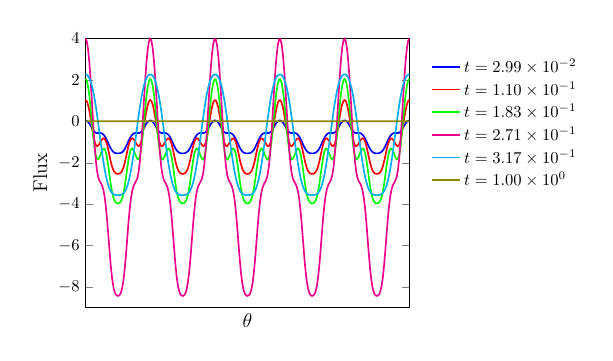
\begin{tikzpicture}[scale=0.6]

  \begin{axis}[
    xmin = 0,
    xmax = 6.2832,
    ymin = -9,
    ymax = 4,
    xtick = \empty,
    ylabel near ticks,
    xlabel = {\large $\theta$},
    ylabel = {\large Flux},
    clip = false,
    legend entries = {$t=2.99 \times 10^{-2}$,
    $t = 1.10 \times 10^{-1}$,
    $t = 1.83 \times 10^{-1}$,
    $t = 2.71 \times 10^{-1}$,
    $t = 3.17 \times 10^{-1}$,
    $t = 1.00 \times 10^{0}$},
    legend cell align=left,
    legend style={draw=none},
    legend style={at={(1.05,0.95)},anchor=north west}
  ]


\addplot[blue,line width=1pt] coordinates{
(0.0000e+00,4.3317e-02)
(2.4544e-02,2.5998e-02)
(4.9087e-02,-2.5040e-02)
(7.3631e-02,-1.0592e-01)
(9.8175e-02,-2.0844e-01)
(1.2272e-01,-3.1903e-01)
(1.4726e-01,-4.2115e-01)
(1.7181e-01,-4.9983e-01)
(1.9635e-01,-5.4734e-01)
(2.2089e-01,-5.6568e-01)
(2.4544e-01,-5.6530e-01)
(2.6998e-01,-5.6032e-01)
(2.9452e-01,-5.6394e-01)
(3.1907e-01,-5.8571e-01)
(3.4361e-01,-6.3142e-01)
(3.6816e-01,-7.0394e-01)
(3.9270e-01,-8.0342e-01)
(4.1724e-01,-9.2582e-01)
(4.4179e-01,-1.0617e+00)
(4.6633e-01,-1.1970e+00)
(4.9087e-01,-1.3173e+00)
(5.1542e-01,-1.4120e+00)
(5.3996e-01,-1.4782e+00)
(5.6450e-01,-1.5185e+00)
(5.8905e-01,-1.5399e+00)
(6.1359e-01,-1.5484e+00)
(6.3814e-01,-1.5494e+00)
(6.6268e-01,-1.5422e+00)
(6.8722e-01,-1.5242e+00)
(7.1177e-01,-1.4880e+00)
(7.3631e-01,-1.4276e+00)
(7.6085e-01,-1.3384e+00)
(7.8540e-01,-1.2228e+00)
(8.0994e-01,-1.0893e+00)
(8.3449e-01,-9.5236e-01)
(8.5903e-01,-8.2627e-01)
(8.8357e-01,-7.2174e-01)
(9.0812e-01,-6.4373e-01)
(9.3266e-01,-5.9279e-01)
(9.5720e-01,-5.6663e-01)
(9.8175e-01,-5.5996e-01)
(1.0063e+00,-5.6425e-01)
(1.0308e+00,-5.6662e-01)
(1.0554e+00,-5.5315e-01)
(1.0799e+00,-5.1185e-01)
(1.1045e+00,-4.3921e-01)
(1.1290e+00,-3.4060e-01)
(1.1536e+00,-2.3049e-01)
(1.1781e+00,-1.2499e-01)
(1.2026e+00,-3.9071e-02)
(1.2272e+00,1.8448e-02)
(1.2517e+00,4.2616e-02)
(1.2763e+00,3.2199e-02)
(1.3008e+00,-1.2223e-02)
(1.3254e+00,-8.7735e-02)
(1.3499e+00,-1.8672e-01)
(1.3744e+00,-2.9711e-01)
(1.3990e+00,-4.0213e-01)
(1.4235e+00,-4.8654e-01)
(1.4481e+00,-5.4032e-01)
(1.4726e+00,-5.6398e-01)
(1.4972e+00,-5.6616e-01)
(1.5217e+00,-5.6104e-01)
(1.5463e+00,-5.6198e-01)
(1.5708e+00,-5.7959e-01)
(1.5953e+00,-6.2017e-01)
(1.6199e+00,-6.8723e-01)
(1.6444e+00,-7.8150e-01)
(1.6690e+00,-8.9986e-01)
(1.6935e+00,-1.0342e+00)
(1.7181e+00,-1.1707e+00)
(1.7426e+00,-1.2951e+00)
(1.7671e+00,-1.3952e+00)
(1.7917e+00,-1.4673e+00)
(1.8162e+00,-1.5120e+00)
(1.8408e+00,-1.5370e+00)
(1.8653e+00,-1.5472e+00)
(1.8899e+00,-1.5500e+00)
(1.9144e+00,-1.5441e+00)
(1.9390e+00,-1.5292e+00)
(1.9635e+00,-1.4968e+00)
(1.9880e+00,-1.4420e+00)
(2.0126e+00,-1.3584e+00)
(2.0371e+00,-1.2478e+00)
(2.0617e+00,-1.1167e+00)
(2.0862e+00,-9.7934e-01)
(2.1108e+00,-8.5000e-01)
(2.1353e+00,-7.4061e-01)
(2.1598e+00,-6.5714e-01)
(2.1844e+00,-6.0088e-01)
(2.2089e+00,-5.7010e-01)
(2.2335e+00,-5.6006e-01)
(2.2580e+00,-5.6311e-01)
(2.2826e+00,-5.6694e-01)
(2.3071e+00,-5.5782e-01)
(2.3317e+00,-5.2259e-01)
(2.3562e+00,-4.5618e-01)
(2.3807e+00,-3.6172e-01)
(2.4053e+00,-2.5272e-01)
(2.4298e+00,-1.4487e-01)
(2.4544e+00,-5.4244e-02)
(2.4789e+00,9.5525e-03)
(2.5035e+00,4.0521e-02)
(2.5280e+00,3.7044e-02)
(2.5525e+00,-6.7853e-04)
(2.5771e+00,-7.0488e-02)
(2.6016e+00,-1.6549e-01)
(2.6262e+00,-2.7497e-01)
(2.6507e+00,-3.8227e-01)
(2.6753e+00,-4.7198e-01)
(2.6998e+00,-5.3208e-01)
(2.7243e+00,-5.6140e-01)
(2.7489e+00,-5.6675e-01)
(2.7734e+00,-5.6201e-01)
(2.7980e+00,-5.6071e-01)
(2.8225e+00,-5.7441e-01)
(2.8471e+00,-6.1000e-01)
(2.8716e+00,-6.7163e-01)
(2.8962e+00,-7.6055e-01)
(2.9207e+00,-8.7456e-01)
(2.9452e+00,-1.0066e+00)
(2.9698e+00,-1.1439e+00)
(2.9943e+00,-1.2719e+00)
(3.0189e+00,-1.3774e+00)
(3.0434e+00,-1.4552e+00)
(3.0680e+00,-1.5048e+00)
(3.0925e+00,-1.5335e+00)
(3.1170e+00,-1.5458e+00)
(3.1416e+00,-1.5502e+00)
(3.1661e+00,-1.5458e+00)
(3.1907e+00,-1.5335e+00)
(3.2152e+00,-1.5048e+00)
(3.2398e+00,-1.4552e+00)
(3.2643e+00,-1.3774e+00)
(3.2889e+00,-1.2719e+00)
(3.3134e+00,-1.1439e+00)
(3.3379e+00,-1.0066e+00)
(3.3625e+00,-8.7455e-01)
(3.3870e+00,-7.6055e-01)
(3.4116e+00,-6.7163e-01)
(3.4361e+00,-6.1000e-01)
(3.4607e+00,-5.7441e-01)
(3.4852e+00,-5.6071e-01)
(3.5097e+00,-5.6201e-01)
(3.5343e+00,-5.6675e-01)
(3.5588e+00,-5.6140e-01)
(3.5834e+00,-5.3208e-01)
(3.6079e+00,-4.7198e-01)
(3.6325e+00,-3.8227e-01)
(3.6570e+00,-2.7497e-01)
(3.6816e+00,-1.6549e-01)
(3.7061e+00,-7.0488e-02)
(3.7306e+00,-6.7871e-04)
(3.7552e+00,3.7044e-02)
(3.7797e+00,4.0521e-02)
(3.8043e+00,9.5528e-03)
(3.8288e+00,-5.4244e-02)
(3.8534e+00,-1.4487e-01)
(3.8779e+00,-2.5272e-01)
(3.9024e+00,-3.6172e-01)
(3.9270e+00,-4.5618e-01)
(3.9515e+00,-5.2259e-01)
(3.9761e+00,-5.5782e-01)
(4.0006e+00,-5.6694e-01)
(4.0252e+00,-5.6311e-01)
(4.0497e+00,-5.6006e-01)
(4.0743e+00,-5.7010e-01)
(4.0988e+00,-6.0088e-01)
(4.1233e+00,-6.5714e-01)
(4.1479e+00,-7.4062e-01)
(4.1724e+00,-8.5000e-01)
(4.1970e+00,-9.7934e-01)
(4.2215e+00,-1.1167e+00)
(4.2461e+00,-1.2478e+00)
(4.2706e+00,-1.3584e+00)
(4.2951e+00,-1.4420e+00)
(4.3197e+00,-1.4968e+00)
(4.3442e+00,-1.5292e+00)
(4.3688e+00,-1.5441e+00)
(4.3933e+00,-1.5500e+00)
(4.4179e+00,-1.5472e+00)
(4.4424e+00,-1.5370e+00)
(4.4670e+00,-1.5120e+00)
(4.4915e+00,-1.4673e+00)
(4.5160e+00,-1.3952e+00)
(4.5406e+00,-1.2951e+00)
(4.5651e+00,-1.1707e+00)
(4.5897e+00,-1.0342e+00)
(4.6142e+00,-8.9986e-01)
(4.6388e+00,-7.8150e-01)
(4.6633e+00,-6.8723e-01)
(4.6878e+00,-6.2017e-01)
(4.7124e+00,-5.7959e-01)
(4.7369e+00,-5.6198e-01)
(4.7615e+00,-5.6104e-01)
(4.7860e+00,-5.6616e-01)
(4.8106e+00,-5.6398e-01)
(4.8351e+00,-5.4032e-01)
(4.8597e+00,-4.8654e-01)
(4.8842e+00,-4.0213e-01)
(4.9087e+00,-2.9711e-01)
(4.9333e+00,-1.8672e-01)
(4.9578e+00,-8.7735e-02)
(4.9824e+00,-1.2223e-02)
(5.0069e+00,3.2199e-02)
(5.0315e+00,4.2616e-02)
(5.0560e+00,1.8448e-02)
(5.0805e+00,-3.9071e-02)
(5.1051e+00,-1.2499e-01)
(5.1296e+00,-2.3049e-01)
(5.1542e+00,-3.4060e-01)
(5.1787e+00,-4.3921e-01)
(5.2033e+00,-5.1185e-01)
(5.2278e+00,-5.5315e-01)
(5.2524e+00,-5.6662e-01)
(5.2769e+00,-5.6425e-01)
(5.3014e+00,-5.5996e-01)
(5.3260e+00,-5.6663e-01)
(5.3505e+00,-5.9279e-01)
(5.3751e+00,-6.4373e-01)
(5.3996e+00,-7.2174e-01)
(5.4242e+00,-8.2627e-01)
(5.4487e+00,-9.5236e-01)
(5.4732e+00,-1.0893e+00)
(5.4978e+00,-1.2228e+00)
(5.5223e+00,-1.3384e+00)
(5.5469e+00,-1.4276e+00)
(5.5714e+00,-1.4880e+00)
(5.5960e+00,-1.5242e+00)
(5.6205e+00,-1.5422e+00)
(5.6450e+00,-1.5494e+00)
(5.6696e+00,-1.5484e+00)
(5.6941e+00,-1.5399e+00)
(5.7187e+00,-1.5185e+00)
(5.7432e+00,-1.4782e+00)
(5.7678e+00,-1.4120e+00)
(5.7923e+00,-1.3173e+00)
(5.8169e+00,-1.1970e+00)
(5.8414e+00,-1.0617e+00)
(5.8659e+00,-9.2582e-01)
(5.8905e+00,-8.0342e-01)
(5.9150e+00,-7.0394e-01)
(5.9396e+00,-6.3142e-01)
(5.9641e+00,-5.8571e-01)
(5.9887e+00,-5.6394e-01)
(6.0132e+00,-5.6032e-01)
(6.0377e+00,-5.6530e-01)
(6.0623e+00,-5.6568e-01)
(6.0868e+00,-5.4734e-01)
(6.1114e+00,-4.9983e-01)
(6.1359e+00,-4.2115e-01)
(6.1605e+00,-3.1903e-01)
(6.1850e+00,-2.0844e-01)
(6.2096e+00,-1.0592e-01)
(6.2341e+00,-2.5040e-02)
(6.2586e+00,2.5998e-02)
(6.2832e+00,4.3317e-02)
};

\addplot[red,line width=1pt] coordinates{
(0.0000e+00,1.0315e+00)
(2.4544e-02,9.7196e-01)
(4.9087e-02,7.9557e-01)
(7.3631e-02,5.1327e-01)
(9.8175e-02,1.4973e-01)
(1.2272e-01,-2.5148e-01)
(1.4726e-01,-6.3351e-01)
(1.7181e-01,-9.3940e-01)
(1.9635e-01,-1.1313e+00)
(2.2089e-01,-1.2017e+00)
(2.4544e-01,-1.1725e+00)
(2.6998e-01,-1.0823e+00)
(2.9452e-01,-9.7242e-01)
(3.1907e-01,-8.7733e-01)
(3.4361e-01,-8.2501e-01)
(3.6816e-01,-8.3886e-01)
(3.9270e-01,-9.3717e-01)
(4.1724e-01,-1.1244e+00)
(4.4179e-01,-1.3839e+00)
(4.6633e-01,-1.6771e+00)
(4.9087e-01,-1.9585e+00)
(5.1542e-01,-2.1904e+00)
(5.3996e-01,-2.3570e+00)
(5.6450e-01,-2.4599e+00)
(5.8905e-01,-2.5151e+00)
(6.1359e-01,-2.5370e+00)
(6.3814e-01,-2.5398e+00)
(6.6268e-01,-2.5209e+00)
(6.8722e-01,-2.4749e+00)
(7.1177e-01,-2.3818e+00)
(7.3631e-01,-2.2295e+00)
(7.6085e-01,-2.0094e+00)
(7.8540e-01,-1.7360e+00)
(8.0994e-01,-1.4411e+00)
(8.3449e-01,-1.1716e+00)
(8.5903e-01,-9.6761e-01)
(8.8357e-01,-8.5140e-01)
(9.0812e-01,-8.2180e-01)
(9.3266e-01,-8.6260e-01)
(9.5720e-01,-9.5131e-01)
(9.8175e-01,-1.0606e+00)
(1.0063e+00,-1.1581e+00)
(1.0308e+00,-1.2025e+00)
(1.0554e+00,-1.1550e+00)
(1.0799e+00,-9.8741e-01)
(1.1045e+00,-7.0261e-01)
(1.1290e+00,-3.3111e-01)
(1.1536e+00,7.0559e-02)
(1.1781e+00,4.4617e-01)
(1.2026e+00,7.4685e-01)
(1.2272e+00,9.4595e-01)
(1.2517e+00,1.0291e+00)
(1.2763e+00,9.9330e-01)
(1.3008e+00,8.3999e-01)
(1.3254e+00,5.7706e-01)
(1.3499e+00,2.2734e-01)
(1.3744e+00,-1.7109e-01)
(1.3990e+00,-5.6129e-01)
(1.4235e+00,-8.8675e-01)
(1.4481e+00,-1.1027e+00)
(1.4726e+00,-1.1968e+00)
(1.4972e+00,-1.1844e+00)
(1.5217e+00,-1.1033e+00)
(1.5463e+00,-9.9412e-01)
(1.5708e+00,-8.9380e-01)
(1.5953e+00,-8.3086e-01)
(1.6199e+00,-8.2977e-01)
(1.6444e+00,-9.1033e-01)
(1.6690e+00,-1.0802e+00)
(1.6935e+00,-1.3280e+00)
(1.7181e+00,-1.6177e+00)
(1.7426e+00,-1.9056e+00)
(1.7671e+00,-2.1486e+00)
(1.7917e+00,-2.3296e+00)
(1.8162e+00,-2.4431e+00)
(1.8408e+00,-2.5079e+00)
(1.8653e+00,-2.5337e+00)
(1.8899e+00,-2.5416e+00)
(1.9144e+00,-2.5257e+00)
(1.9390e+00,-2.4879e+00)
(1.9635e+00,-2.4042e+00)
(1.9880e+00,-2.2658e+00)
(2.0126e+00,-2.0580e+00)
(2.0371e+00,-1.7940e+00)
(2.0617e+00,-1.4994e+00)
(2.0862e+00,-1.2215e+00)
(2.1108e+00,-1.0016e+00)
(2.1353e+00,-8.6746e-01)
(2.1598e+00,-8.2140e-01)
(2.1844e+00,-8.4982e-01)
(2.2089e+00,-9.3102e-01)
(2.2335e+00,-1.0385e+00)
(2.2580e+00,-1.1415e+00)
(2.2826e+00,-1.1997e+00)
(2.3071e+00,-1.1737e+00)
(2.3317e+00,-1.0307e+00)
(2.3562e+00,-7.6810e-01)
(2.3807e+00,-4.0959e-01)
(2.4053e+00,-9.6323e-03)
(2.4298e+00,3.7596e-01)
(2.4544e+00,6.9405e-01)
(2.4789e+00,9.1527e-01)
(2.5035e+00,1.0219e+00)
(2.5280e+00,1.0100e+00)
(2.5525e+00,8.7993e-01)
(2.5771e+00,6.3738e-01)
(2.6016e+00,3.0290e-01)
(2.6262e+00,-9.0337e-02)
(2.6507e+00,-4.8648e-01)
(2.6753e+00,-8.2958e-01)
(2.6998e+00,-1.0691e+00)
(2.7243e+00,-1.1876e+00)
(2.7489e+00,-1.1936e+00)
(2.7734e+00,-1.1231e+00)
(2.7980e+00,-1.0162e+00)
(2.8225e+00,-9.1177e-01)
(2.8471e+00,-8.3919e-01)
(2.8716e+00,-8.2400e-01)
(2.8962e+00,-8.8710e-01)
(2.9207e+00,-1.0392e+00)
(2.9452e+00,-1.2738e+00)
(2.9698e+00,-1.5584e+00)
(2.9943e+00,-1.8507e+00)
(3.0189e+00,-2.1045e+00)
(3.0434e+00,-2.2992e+00)
(3.0680e+00,-2.4246e+00)
(3.0925e+00,-2.4989e+00)
(3.1170e+00,-2.5299e+00)
(3.1416e+00,-2.5423e+00)
(3.1661e+00,-2.5299e+00)
(3.1907e+00,-2.4989e+00)
(3.2152e+00,-2.4246e+00)
(3.2398e+00,-2.2992e+00)
(3.2643e+00,-2.1045e+00)
(3.2889e+00,-1.8507e+00)
(3.3134e+00,-1.5584e+00)
(3.3379e+00,-1.2738e+00)
(3.3625e+00,-1.0392e+00)
(3.3870e+00,-8.8710e-01)
(3.4116e+00,-8.2400e-01)
(3.4361e+00,-8.3919e-01)
(3.4607e+00,-9.1177e-01)
(3.4852e+00,-1.0162e+00)
(3.5097e+00,-1.1231e+00)
(3.5343e+00,-1.1936e+00)
(3.5588e+00,-1.1876e+00)
(3.5834e+00,-1.0691e+00)
(3.6079e+00,-8.2958e-01)
(3.6325e+00,-4.8648e-01)
(3.6570e+00,-9.0337e-02)
(3.6816e+00,3.0290e-01)
(3.7061e+00,6.3738e-01)
(3.7306e+00,8.7993e-01)
(3.7552e+00,1.0100e+00)
(3.7797e+00,1.0219e+00)
(3.8043e+00,9.1527e-01)
(3.8288e+00,6.9405e-01)
(3.8534e+00,3.7596e-01)
(3.8779e+00,-9.6323e-03)
(3.9024e+00,-4.0959e-01)
(3.9270e+00,-7.6810e-01)
(3.9515e+00,-1.0307e+00)
(3.9761e+00,-1.1737e+00)
(4.0006e+00,-1.1997e+00)
(4.0252e+00,-1.1415e+00)
(4.0497e+00,-1.0385e+00)
(4.0743e+00,-9.3102e-01)
(4.0988e+00,-8.4982e-01)
(4.1233e+00,-8.2140e-01)
(4.1479e+00,-8.6746e-01)
(4.1724e+00,-1.0016e+00)
(4.1970e+00,-1.2215e+00)
(4.2215e+00,-1.4994e+00)
(4.2461e+00,-1.7940e+00)
(4.2706e+00,-2.0580e+00)
(4.2951e+00,-2.2658e+00)
(4.3197e+00,-2.4042e+00)
(4.3442e+00,-2.4879e+00)
(4.3688e+00,-2.5257e+00)
(4.3933e+00,-2.5416e+00)
(4.4179e+00,-2.5337e+00)
(4.4424e+00,-2.5079e+00)
(4.4670e+00,-2.4431e+00)
(4.4915e+00,-2.3296e+00)
(4.5160e+00,-2.1486e+00)
(4.5406e+00,-1.9056e+00)
(4.5651e+00,-1.6177e+00)
(4.5897e+00,-1.3280e+00)
(4.6142e+00,-1.0802e+00)
(4.6388e+00,-9.1033e-01)
(4.6633e+00,-8.2977e-01)
(4.6878e+00,-8.3086e-01)
(4.7124e+00,-8.9380e-01)
(4.7369e+00,-9.9412e-01)
(4.7615e+00,-1.1033e+00)
(4.7860e+00,-1.1844e+00)
(4.8106e+00,-1.1968e+00)
(4.8351e+00,-1.1027e+00)
(4.8597e+00,-8.8675e-01)
(4.8842e+00,-5.6129e-01)
(4.9087e+00,-1.7109e-01)
(4.9333e+00,2.2734e-01)
(4.9578e+00,5.7706e-01)
(4.9824e+00,8.3999e-01)
(5.0069e+00,9.9330e-01)
(5.0315e+00,1.0291e+00)
(5.0560e+00,9.4595e-01)
(5.0805e+00,7.4685e-01)
(5.1051e+00,4.4617e-01)
(5.1296e+00,7.0559e-02)
(5.1542e+00,-3.3111e-01)
(5.1787e+00,-7.0261e-01)
(5.2033e+00,-9.8741e-01)
(5.2278e+00,-1.1550e+00)
(5.2524e+00,-1.2025e+00)
(5.2769e+00,-1.1581e+00)
(5.3014e+00,-1.0606e+00)
(5.3260e+00,-9.5131e-01)
(5.3505e+00,-8.6260e-01)
(5.3751e+00,-8.2180e-01)
(5.3996e+00,-8.5140e-01)
(5.4242e+00,-9.6761e-01)
(5.4487e+00,-1.1716e+00)
(5.4732e+00,-1.4411e+00)
(5.4978e+00,-1.7360e+00)
(5.5223e+00,-2.0094e+00)
(5.5469e+00,-2.2295e+00)
(5.5714e+00,-2.3818e+00)
(5.5960e+00,-2.4749e+00)
(5.6205e+00,-2.5209e+00)
(5.6450e+00,-2.5398e+00)
(5.6696e+00,-2.5370e+00)
(5.6941e+00,-2.5151e+00)
(5.7187e+00,-2.4599e+00)
(5.7432e+00,-2.3570e+00)
(5.7678e+00,-2.1904e+00)
(5.7923e+00,-1.9585e+00)
(5.8169e+00,-1.6771e+00)
(5.8414e+00,-1.3839e+00)
(5.8659e+00,-1.1244e+00)
(5.8905e+00,-9.3717e-01)
(5.9150e+00,-8.3886e-01)
(5.9396e+00,-8.2501e-01)
(5.9641e+00,-8.7733e-01)
(5.9887e+00,-9.7242e-01)
(6.0132e+00,-1.0823e+00)
(6.0377e+00,-1.1725e+00)
(6.0623e+00,-1.2017e+00)
(6.0868e+00,-1.1313e+00)
(6.1114e+00,-9.3940e-01)
(6.1359e+00,-6.3351e-01)
(6.1605e+00,-2.5148e-01)
(6.1850e+00,1.4973e-01)
(6.2096e+00,5.1327e-01)
(6.2341e+00,7.9557e-01)
(6.2586e+00,9.7196e-01)
(6.2832e+00,1.0315e+00)
};

\addplot[green,line width=1pt] coordinates{
(0.0000e+00,2.0503e+00)
(2.4544e-02,1.9579e+00)
(4.9087e-02,1.6826e+00)
(7.3631e-02,1.2369e+00)
(9.8175e-02,6.5244e-01)
(1.2272e-01,-1.0525e-02)
(1.4726e-01,-6.6768e-01)
(1.7181e-01,-1.2271e+00)
(1.9635e-01,-1.6187e+00)
(2.2089e-01,-1.8145e+00)
(2.4544e-01,-1.8351e+00)
(2.6998e-01,-1.7337e+00)
(2.9452e-01,-1.5761e+00)
(3.1907e-01,-1.4227e+00)
(3.4361e-01,-1.3265e+00)
(3.6816e-01,-1.3323e+00)
(3.9270e-01,-1.4744e+00)
(4.1724e-01,-1.7612e+00)
(4.4179e-01,-2.1652e+00)
(4.6633e-01,-2.6230e+00)
(4.9087e-01,-3.0621e+00)
(5.1542e-01,-3.4228e+00)
(5.3996e-01,-3.6817e+00)
(5.6450e-01,-3.8410e+00)
(5.8905e-01,-3.9267e+00)
(6.1359e-01,-3.9605e+00)
(6.3814e-01,-3.9649e+00)
(6.6268e-01,-3.9355e+00)
(6.8722e-01,-3.8644e+00)
(7.1177e-01,-3.7199e+00)
(7.3631e-01,-3.4837e+00)
(7.6085e-01,-3.1411e+00)
(7.8540e-01,-2.7151e+00)
(8.0994e-01,-2.2545e+00)
(8.3449e-01,-1.8345e+00)
(8.5903e-01,-1.5203e+00)
(8.8357e-01,-1.3491e+00)
(9.0812e-01,-1.3182e+00)
(9.3266e-01,-1.3973e+00)
(9.5720e-01,-1.5434e+00)
(9.8175e-01,-1.7045e+00)
(1.0063e+00,-1.8227e+00)
(1.0308e+00,-1.8310e+00)
(1.0554e+00,-1.6739e+00)
(1.0799e+00,-1.3201e+00)
(1.1045e+00,-7.9051e-01)
(1.1290e+00,-1.4500e-01)
(1.1536e+00,5.2329e-01)
(1.1781e+00,1.1300e+00)
(1.2026e+00,1.6061e+00)
(1.2272e+00,1.9174e+00)
(1.2517e+00,2.0466e+00)
(1.2763e+00,1.9910e+00)
(1.3008e+00,1.7521e+00)
(1.3254e+00,1.3382e+00)
(1.3499e+00,7.7837e-01)
(1.3744e+00,1.2414e-01)
(1.3990e+00,-5.4084e-01)
(1.4235e+00,-1.1273e+00)
(1.4481e+00,-1.5556e+00)
(1.4726e+00,-1.7909e+00)
(1.4972e+00,-1.8425e+00)
(1.5217e+00,-1.7608e+00)
(1.5463e+00,-1.6090e+00)
(1.5708e+00,-1.4505e+00)
(1.5953e+00,-1.3390e+00)
(1.6199e+00,-1.3210e+00)
(1.6444e+00,-1.4343e+00)
(1.6690e+00,-1.6927e+00)
(1.6935e+00,-2.0781e+00)
(1.7181e+00,-2.5302e+00)
(1.7426e+00,-2.9797e+00)
(1.7671e+00,-3.3577e+00)
(1.7917e+00,-3.6392e+00)
(1.8162e+00,-3.8149e+00)
(1.8408e+00,-3.9157e+00)
(1.8653e+00,-3.9552e+00)
(1.8899e+00,-3.9678e+00)
(1.9144e+00,-3.9428e+00)
(1.9390e+00,-3.8847e+00)
(1.9635e+00,-3.7545e+00)
(1.9880e+00,-3.5403e+00)
(2.0126e+00,-3.2168e+00)
(2.0371e+00,-2.8057e+00)
(2.0617e+00,-2.3454e+00)
(2.0862e+00,-1.9122e+00)
(2.1108e+00,-1.5721e+00)
(2.1353e+00,-1.3717e+00)
(2.1598e+00,-1.3142e+00)
(2.1844e+00,-1.3747e+00)
(2.2089e+00,-1.5113e+00)
(2.2335e+00,-1.6736e+00)
(2.2580e+00,-1.8059e+00)
(2.2826e+00,-1.8409e+00)
(2.3071e+00,-1.7209e+00)
(2.3317e+00,-1.4060e+00)
(2.3562e+00,-9.0851e-01)
(2.3807e+00,-2.7869e-01)
(2.4053e+00,3.9170e-01)
(2.4298e+00,1.0177e+00)
(2.4544e+00,1.5230e+00)
(2.4789e+00,1.8696e+00)
(2.5035e+00,2.0354e+00)
(2.5280e+00,2.0169e+00)
(2.5525e+00,1.8145e+00)
(2.5771e+00,1.4336e+00)
(2.6016e+00,9.0034e-01)
(2.6262e+00,2.5842e-01)
(2.6507e+00,-4.1089e-01)
(2.6753e+00,-1.0210e+00)
(2.6998e+00,-1.4846e+00)
(2.7243e+00,-1.7598e+00)
(2.7489e+00,-1.8446e+00)
(2.7734e+00,-1.7850e+00)
(2.7980e+00,-1.6416e+00)
(2.8225e+00,-1.4801e+00)
(2.8471e+00,-1.3551e+00)
(2.8716e+00,-1.3150e+00)
(2.8962e+00,-1.4001e+00)
(2.9207e+00,-1.6296e+00)
(2.9452e+00,-1.9936e+00)
(2.9698e+00,-2.4375e+00)
(2.9943e+00,-2.8941e+00)
(3.0189e+00,-3.2890e+00)
(3.0434e+00,-3.5921e+00)
(3.0680e+00,-3.7861e+00)
(3.0925e+00,-3.9018e+00)
(3.1170e+00,-3.9493e+00)
(3.1416e+00,-3.9688e+00)
(3.1661e+00,-3.9493e+00)
(3.1907e+00,-3.9018e+00)
(3.2152e+00,-3.7861e+00)
(3.2398e+00,-3.5921e+00)
(3.2643e+00,-3.2890e+00)
(3.2889e+00,-2.8941e+00)
(3.3134e+00,-2.4375e+00)
(3.3379e+00,-1.9936e+00)
(3.3625e+00,-1.6296e+00)
(3.3870e+00,-1.4001e+00)
(3.4116e+00,-1.3150e+00)
(3.4361e+00,-1.3551e+00)
(3.4607e+00,-1.4801e+00)
(3.4852e+00,-1.6416e+00)
(3.5097e+00,-1.7850e+00)
(3.5343e+00,-1.8446e+00)
(3.5588e+00,-1.7598e+00)
(3.5834e+00,-1.4846e+00)
(3.6079e+00,-1.0210e+00)
(3.6325e+00,-4.1090e-01)
(3.6570e+00,2.5842e-01)
(3.6816e+00,9.0034e-01)
(3.7061e+00,1.4336e+00)
(3.7306e+00,1.8145e+00)
(3.7552e+00,2.0169e+00)
(3.7797e+00,2.0354e+00)
(3.8043e+00,1.8696e+00)
(3.8288e+00,1.5230e+00)
(3.8534e+00,1.0177e+00)
(3.8779e+00,3.9170e-01)
(3.9024e+00,-2.7869e-01)
(3.9270e+00,-9.0851e-01)
(3.9515e+00,-1.4060e+00)
(3.9761e+00,-1.7209e+00)
(4.0006e+00,-1.8409e+00)
(4.0252e+00,-1.8059e+00)
(4.0497e+00,-1.6736e+00)
(4.0743e+00,-1.5113e+00)
(4.0988e+00,-1.3747e+00)
(4.1233e+00,-1.3142e+00)
(4.1479e+00,-1.3717e+00)
(4.1724e+00,-1.5721e+00)
(4.1970e+00,-1.9122e+00)
(4.2215e+00,-2.3454e+00)
(4.2461e+00,-2.8057e+00)
(4.2706e+00,-3.2168e+00)
(4.2951e+00,-3.5403e+00)
(4.3197e+00,-3.7545e+00)
(4.3442e+00,-3.8847e+00)
(4.3688e+00,-3.9428e+00)
(4.3933e+00,-3.9678e+00)
(4.4179e+00,-3.9552e+00)
(4.4424e+00,-3.9157e+00)
(4.4670e+00,-3.8149e+00)
(4.4915e+00,-3.6392e+00)
(4.5160e+00,-3.3577e+00)
(4.5406e+00,-2.9797e+00)
(4.5651e+00,-2.5302e+00)
(4.5897e+00,-2.0781e+00)
(4.6142e+00,-1.6927e+00)
(4.6388e+00,-1.4343e+00)
(4.6633e+00,-1.3210e+00)
(4.6878e+00,-1.3390e+00)
(4.7124e+00,-1.4505e+00)
(4.7369e+00,-1.6090e+00)
(4.7615e+00,-1.7608e+00)
(4.7860e+00,-1.8425e+00)
(4.8106e+00,-1.7909e+00)
(4.8351e+00,-1.5556e+00)
(4.8597e+00,-1.1273e+00)
(4.8842e+00,-5.4084e-01)
(4.9087e+00,1.2414e-01)
(4.9333e+00,7.7837e-01)
(4.9578e+00,1.3382e+00)
(4.9824e+00,1.7521e+00)
(5.0069e+00,1.9910e+00)
(5.0315e+00,2.0466e+00)
(5.0560e+00,1.9174e+00)
(5.0805e+00,1.6061e+00)
(5.1051e+00,1.1300e+00)
(5.1296e+00,5.2329e-01)
(5.1542e+00,-1.4500e-01)
(5.1787e+00,-7.9051e-01)
(5.2033e+00,-1.3201e+00)
(5.2278e+00,-1.6739e+00)
(5.2524e+00,-1.8310e+00)
(5.2769e+00,-1.8227e+00)
(5.3014e+00,-1.7045e+00)
(5.3260e+00,-1.5434e+00)
(5.3505e+00,-1.3973e+00)
(5.3751e+00,-1.3182e+00)
(5.3996e+00,-1.3491e+00)
(5.4242e+00,-1.5203e+00)
(5.4487e+00,-1.8345e+00)
(5.4732e+00,-2.2545e+00)
(5.4978e+00,-2.7151e+00)
(5.5223e+00,-3.1411e+00)
(5.5469e+00,-3.4837e+00)
(5.5714e+00,-3.7199e+00)
(5.5960e+00,-3.8644e+00)
(5.6205e+00,-3.9355e+00)
(5.6450e+00,-3.9649e+00)
(5.6696e+00,-3.9605e+00)
(5.6941e+00,-3.9267e+00)
(5.7187e+00,-3.8410e+00)
(5.7432e+00,-3.6817e+00)
(5.7678e+00,-3.4228e+00)
(5.7923e+00,-3.0621e+00)
(5.8169e+00,-2.6230e+00)
(5.8414e+00,-2.1652e+00)
(5.8659e+00,-1.7612e+00)
(5.8905e+00,-1.4744e+00)
(5.9150e+00,-1.3323e+00)
(5.9396e+00,-1.3265e+00)
(5.9641e+00,-1.4227e+00)
(5.9887e+00,-1.5761e+00)
(6.0132e+00,-1.7337e+00)
(6.0377e+00,-1.8351e+00)
(6.0623e+00,-1.8145e+00)
(6.0868e+00,-1.6187e+00)
(6.1114e+00,-1.2271e+00)
(6.1359e+00,-6.6768e-01)
(6.1605e+00,-1.0525e-02)
(6.1850e+00,6.5244e-01)
(6.2096e+00,1.2369e+00)
(6.2341e+00,1.6826e+00)
(6.2586e+00,1.9579e+00)
(6.2832e+00,2.0503e+00)
};

\addplot[magenta,line width=1pt] coordinates{
(0.0000e+00,3.9993e+00)
(2.4544e-02,3.8712e+00)
(4.9087e-02,3.4877e+00)
(7.3631e-02,2.8573e+00)
(9.8175e-02,2.0100e+00)
(1.2272e-01,1.0122e+00)
(1.4726e-01,-3.3804e-02)
(1.7181e-01,-1.0057e+00)
(1.9635e-01,-1.7982e+00)
(2.2089e-01,-2.3554e+00)
(2.4544e-01,-2.6897e+00)
(2.6998e-01,-2.8661e+00)
(2.9452e-01,-2.9732e+00)
(3.1907e-01,-3.0909e+00)
(3.4361e-01,-3.2837e+00)
(3.6816e-01,-3.6001e+00)
(3.9270e-01,-4.0770e+00)
(4.1724e-01,-4.7175e+00)
(4.4179e-01,-5.4796e+00)
(4.6633e-01,-6.2730e+00)
(4.9087e-01,-6.9993e+00)
(5.1542e-01,-7.5802e+00)
(5.3996e-01,-7.9905e+00)
(5.6450e-01,-8.2411e+00)
(5.8905e-01,-8.3747e+00)
(6.1359e-01,-8.4281e+00)
(6.3814e-01,-8.4340e+00)
(6.6268e-01,-8.3891e+00)
(6.8722e-01,-8.2773e+00)
(7.1177e-01,-8.0510e+00)
(7.3631e-01,-7.6771e+00)
(7.6085e-01,-7.1278e+00)
(7.8540e-01,-6.4275e+00)
(8.0994e-01,-5.6385e+00)
(8.3449e-01,-4.8630e+00)
(8.5903e-01,-4.1923e+00)
(8.8357e-01,-3.6822e+00)
(9.0812e-01,-3.3355e+00)
(9.3266e-01,-3.1217e+00)
(9.5720e-01,-2.9937e+00)
(9.8175e-01,-2.8900e+00)
(1.0063e+00,-2.7351e+00)
(1.0308e+00,-2.4382e+00)
(1.0554e+00,-1.9294e+00)
(1.0799e+00,-1.1808e+00)
(1.1045e+00,-2.3848e-01)
(1.1290e+00,8.0355e-01)
(1.1536e+00,1.8192e+00)
(1.1781e+00,2.7041e+00)
(1.2026e+00,3.3804e+00)
(1.2272e+00,3.8151e+00)
(1.2517e+00,3.9941e+00)
(1.2763e+00,3.9172e+00)
(1.3008e+00,3.5850e+00)
(1.3254e+00,3.0017e+00)
(1.3499e+00,2.1947e+00)
(1.3744e+00,1.2188e+00)
(1.3990e+00,1.7391e-01)
(1.4235e+00,-8.2334e-01)
(1.4481e+00,-1.6572e+00)
(1.4726e+00,-2.2634e+00)
(1.4972e+00,-2.6378e+00)
(1.5217e+00,-2.8394e+00)
(1.5463e+00,-2.9531e+00)
(1.5708e+00,-3.0632e+00)
(1.5953e+00,-3.2367e+00)
(1.6199e+00,-3.5247e+00)
(1.6444e+00,-3.9684e+00)
(1.6690e+00,-4.5771e+00)
(1.6935e+00,-5.3219e+00)
(1.7181e+00,-6.1160e+00)
(1.7426e+00,-6.8648e+00)
(1.7671e+00,-7.4764e+00)
(1.7917e+00,-7.9234e+00)
(1.8162e+00,-8.2003e+00)
(1.8408e+00,-8.3570e+00)
(1.8653e+00,-8.4205e+00)
(1.8899e+00,-8.4378e+00)
(1.9144e+00,-8.4011e+00)
(1.9390e+00,-8.3087e+00)
(1.9635e+00,-8.1057e+00)
(1.9880e+00,-7.7668e+00)
(2.0126e+00,-7.2501e+00)
(2.0371e+00,-6.5782e+00)
(2.0617e+00,-5.7979e+00)
(2.0862e+00,-5.0128e+00)
(2.1108e+00,-4.3142e+00)
(2.1353e+00,-3.7709e+00)
(2.1598e+00,-3.3927e+00)
(2.1844e+00,-3.1560e+00)
(2.2089e+00,-3.0151e+00)
(2.2335e+00,-2.9121e+00)
(2.2580e+00,-2.7748e+00)
(2.2826e+00,-2.5126e+00)
(2.3071e+00,-2.0507e+00)
(2.3317e+00,-1.3480e+00)
(2.3562e+00,-4.3895e-01)
(2.3807e+00,5.9368e-01)
(2.4053e+00,1.6231e+00)
(2.4298e+00,2.5424e+00)
(2.4544e+00,3.2635e+00)
(2.4789e+00,3.7487e+00)
(2.5035e+00,3.9787e+00)
(2.5280e+00,3.9530e+00)
(2.5525e+00,3.6720e+00)
(2.5771e+00,3.1371e+00)
(2.6016e+00,2.3724e+00)
(2.6262e+00,1.4227e+00)
(2.6507e+00,3.8346e-01)
(2.6753e+00,-6.3419e-01)
(2.6998e+00,-1.5070e+00)
(2.7243e+00,-2.1620e+00)
(2.7489e+00,-2.5789e+00)
(2.7734e+00,-2.8093e+00)
(2.7980e+00,-2.9329e+00)
(2.8225e+00,-3.0381e+00)
(2.8471e+00,-3.1943e+00)
(2.8716e+00,-3.4557e+00)
(2.8962e+00,-3.8663e+00)
(2.9207e+00,-4.4425e+00)
(2.9452e+00,-5.1661e+00)
(2.9698e+00,-5.9573e+00)
(2.9943e+00,-6.7242e+00)
(3.0189e+00,-7.3663e+00)
(3.0434e+00,-7.8489e+00)
(3.0680e+00,-8.1553e+00)
(3.0925e+00,-8.3352e+00)
(3.1170e+00,-8.4114e+00)
(3.1416e+00,-8.4391e+00)
(3.1661e+00,-8.4114e+00)
(3.1907e+00,-8.3353e+00)
(3.2152e+00,-8.1553e+00)
(3.2398e+00,-7.8489e+00)
(3.2643e+00,-7.3663e+00)
(3.2889e+00,-6.7242e+00)
(3.3134e+00,-5.9573e+00)
(3.3379e+00,-5.1661e+00)
(3.3625e+00,-4.4425e+00)
(3.3870e+00,-3.8663e+00)
(3.4116e+00,-3.4557e+00)
(3.4361e+00,-3.1943e+00)
(3.4607e+00,-3.0381e+00)
(3.4852e+00,-2.9329e+00)
(3.5097e+00,-2.8093e+00)
(3.5343e+00,-2.5789e+00)
(3.5588e+00,-2.1620e+00)
(3.5834e+00,-1.5070e+00)
(3.6079e+00,-6.3419e-01)
(3.6325e+00,3.8346e-01)
(3.6570e+00,1.4227e+00)
(3.6816e+00,2.3724e+00)
(3.7061e+00,3.1371e+00)
(3.7306e+00,3.6720e+00)
(3.7552e+00,3.9530e+00)
(3.7797e+00,3.9787e+00)
(3.8043e+00,3.7487e+00)
(3.8288e+00,3.2635e+00)
(3.8534e+00,2.5424e+00)
(3.8779e+00,1.6231e+00)
(3.9024e+00,5.9368e-01)
(3.9270e+00,-4.3895e-01)
(3.9515e+00,-1.3480e+00)
(3.9761e+00,-2.0507e+00)
(4.0006e+00,-2.5126e+00)
(4.0252e+00,-2.7748e+00)
(4.0497e+00,-2.9121e+00)
(4.0743e+00,-3.0151e+00)
(4.0988e+00,-3.1560e+00)
(4.1233e+00,-3.3927e+00)
(4.1479e+00,-3.7709e+00)
(4.1724e+00,-4.3142e+00)
(4.1970e+00,-5.0128e+00)
(4.2215e+00,-5.7979e+00)
(4.2461e+00,-6.5782e+00)
(4.2706e+00,-7.2501e+00)
(4.2951e+00,-7.7668e+00)
(4.3197e+00,-8.1057e+00)
(4.3442e+00,-8.3087e+00)
(4.3688e+00,-8.4011e+00)
(4.3933e+00,-8.4378e+00)
(4.4179e+00,-8.4205e+00)
(4.4424e+00,-8.3570e+00)
(4.4670e+00,-8.2003e+00)
(4.4915e+00,-7.9234e+00)
(4.5160e+00,-7.4764e+00)
(4.5406e+00,-6.8648e+00)
(4.5651e+00,-6.1160e+00)
(4.5897e+00,-5.3219e+00)
(4.6142e+00,-4.5771e+00)
(4.6388e+00,-3.9684e+00)
(4.6633e+00,-3.5247e+00)
(4.6878e+00,-3.2367e+00)
(4.7124e+00,-3.0632e+00)
(4.7369e+00,-2.9531e+00)
(4.7615e+00,-2.8394e+00)
(4.7860e+00,-2.6378e+00)
(4.8106e+00,-2.2634e+00)
(4.8351e+00,-1.6572e+00)
(4.8597e+00,-8.2334e-01)
(4.8842e+00,1.7391e-01)
(4.9087e+00,1.2188e+00)
(4.9333e+00,2.1947e+00)
(4.9578e+00,3.0017e+00)
(4.9824e+00,3.5850e+00)
(5.0069e+00,3.9172e+00)
(5.0315e+00,3.9941e+00)
(5.0560e+00,3.8151e+00)
(5.0805e+00,3.3804e+00)
(5.1051e+00,2.7041e+00)
(5.1296e+00,1.8192e+00)
(5.1542e+00,8.0355e-01)
(5.1787e+00,-2.3848e-01)
(5.2033e+00,-1.1808e+00)
(5.2278e+00,-1.9294e+00)
(5.2524e+00,-2.4382e+00)
(5.2769e+00,-2.7351e+00)
(5.3014e+00,-2.8900e+00)
(5.3260e+00,-2.9937e+00)
(5.3505e+00,-3.1217e+00)
(5.3751e+00,-3.3355e+00)
(5.3996e+00,-3.6822e+00)
(5.4242e+00,-4.1923e+00)
(5.4487e+00,-4.8630e+00)
(5.4732e+00,-5.6385e+00)
(5.4978e+00,-6.4275e+00)
(5.5223e+00,-7.1278e+00)
(5.5469e+00,-7.6771e+00)
(5.5714e+00,-8.0510e+00)
(5.5960e+00,-8.2773e+00)
(5.6205e+00,-8.3891e+00)
(5.6450e+00,-8.4340e+00)
(5.6696e+00,-8.4281e+00)
(5.6941e+00,-8.3747e+00)
(5.7187e+00,-8.2411e+00)
(5.7432e+00,-7.9905e+00)
(5.7678e+00,-7.5802e+00)
(5.7923e+00,-6.9993e+00)
(5.8169e+00,-6.2730e+00)
(5.8414e+00,-5.4796e+00)
(5.8659e+00,-4.7175e+00)
(5.8905e+00,-4.0770e+00)
(5.9150e+00,-3.6001e+00)
(5.9396e+00,-3.2837e+00)
(5.9641e+00,-3.0909e+00)
(5.9887e+00,-2.9732e+00)
(6.0132e+00,-2.8661e+00)
(6.0377e+00,-2.6897e+00)
(6.0623e+00,-2.3554e+00)
(6.0868e+00,-1.7982e+00)
(6.1114e+00,-1.0057e+00)
(6.1359e+00,-3.3804e-02)
(6.1605e+00,1.0122e+00)
(6.1850e+00,2.0100e+00)
(6.2096e+00,2.8573e+00)
(6.2341e+00,3.4877e+00)
(6.2586e+00,3.8712e+00)
(6.2832e+00,3.9993e+00)
};

\addplot[cyan,line width=1pt] coordinates{
(0.0000e+00,2.2712e+00)
(2.4544e-02,2.2523e+00)
(4.9087e-02,2.1939e+00)
(7.3631e-02,2.0920e+00)
(9.8175e-02,1.9409e+00)
(1.2272e-01,1.7354e+00)
(1.4726e-01,1.4720e+00)
(1.7181e-01,1.1508e+00)
(1.9635e-01,7.7631e-01)
(2.2089e-01,3.5743e-01)
(2.4544e-01,-9.3181e-02)
(2.6998e-01,-5.6018e-01)
(2.9452e-01,-1.0272e+00)
(3.1907e-01,-1.4781e+00)
(3.4361e-01,-1.8986e+00)
(3.6816e-01,-2.2769e+00)
(3.9270e-01,-2.6049e+00)
(4.1724e-01,-2.8783e+00)
(4.4179e-01,-3.0966e+00)
(4.6633e-01,-3.2630e+00)
(4.9087e-01,-3.3831e+00)
(5.1542e-01,-3.4648e+00)
(5.3996e-01,-3.5162e+00)
(5.6450e-01,-3.5459e+00)
(5.8905e-01,-3.5608e+00)
(6.1359e-01,-3.5670e+00)
(6.3814e-01,-3.5674e+00)
(6.6268e-01,-3.5627e+00)
(6.8722e-01,-3.5498e+00)
(7.1177e-01,-3.5237e+00)
(7.3631e-01,-3.4772e+00)
(7.6085e-01,-3.4023e+00)
(7.8540e-01,-3.2905e+00)
(8.0994e-01,-3.1339e+00)
(8.3449e-01,-2.9263e+00)
(8.5903e-01,-2.6641e+00)
(8.8357e-01,-2.3467e+00)
(9.0812e-01,-1.9779e+00)
(9.3266e-01,-1.5650e+00)
(9.5720e-01,-1.1191e+00)
(9.8175e-01,-6.5410e-01)
(1.0063e+00,-1.8579e-01)
(1.0308e+00,2.6938e-01)
(1.0554e+00,6.9573e-01)
(1.0799e+00,1.0799e+00)
(1.1045e+00,1.4123e+00)
(1.1290e+00,1.6874e+00)
(1.1536e+00,1.9043e+00)
(1.1781e+00,2.0659e+00)
(1.2026e+00,2.1772e+00)
(1.2272e+00,2.2439e+00)
(1.2517e+00,2.2705e+00)
(1.2763e+00,2.2591e+00)
(1.3008e+00,2.2089e+00)
(1.3254e+00,2.1162e+00)
(1.3499e+00,1.9753e+00)
(1.3744e+00,1.7811e+00)
(1.3990e+00,1.5293e+00)
(1.4235e+00,1.2195e+00)
(1.4481e+00,8.5510e-01)
(1.4726e+00,4.4419e-01)
(1.4972e+00,-1.2315e-03)
(1.5217e+00,-4.6625e-01)
(1.5463e+00,-9.3456e-01)
(1.5708e+00,-1.3899e+00)
(1.5953e+00,-1.8175e+00)
(1.6199e+00,-2.2051e+00)
(1.6444e+00,-2.5436e+00)
(1.6690e+00,-2.8281e+00)
(1.6935e+00,-3.0573e+00)
(1.7181e+00,-3.2336e+00)
(1.7426e+00,-3.3624e+00)
(1.7671e+00,-3.4511e+00)
(1.7917e+00,-3.5079e+00)
(1.8162e+00,-3.5413e+00)
(1.8408e+00,-3.5586e+00)
(1.8653e+00,-3.5663e+00)
(1.8899e+00,-3.5676e+00)
(1.9144e+00,-3.5642e+00)
(1.9390e+00,-3.5532e+00)
(1.9635e+00,-3.5303e+00)
(1.9880e+00,-3.4885e+00)
(2.0126e+00,-3.4200e+00)
(2.0371e+00,-3.3162e+00)
(2.0617e+00,-3.1692e+00)
(2.0862e+00,-2.9721e+00)
(2.1108e+00,-2.7210e+00)
(2.1353e+00,-2.4145e+00)
(2.1598e+00,-2.0555e+00)
(2.1844e+00,-1.6507e+00)
(2.2089e+00,-1.2103e+00)
(2.2335e+00,-7.4789e-01)
(2.2580e+00,-2.7892e-01)
(2.2826e+00,1.8018e-01)
(2.3071e+00,6.1345e-01)
(2.3317e+00,1.0070e+00)
(2.3562e+00,1.3503e+00)
(2.3807e+00,1.6370e+00)
(2.4053e+00,1.8655e+00)
(2.4298e+00,2.0378e+00)
(2.4544e+00,2.1587e+00)
(2.4789e+00,2.2339e+00)
(2.5035e+00,2.2682e+00)
(2.5280e+00,2.2644e+00)
(2.5525e+00,2.2222e+00)
(2.5771e+00,2.1384e+00)
(2.6016e+00,2.0076e+00)
(2.6262e+00,1.8244e+00)
(2.6507e+00,1.5844e+00)
(2.6753e+00,1.2860e+00)
(2.6998e+00,9.3203e-01)
(2.7243e+00,5.2957e-01)
(2.7489e+00,8.9930e-02)
(2.7734e+00,-3.7245e-01)
(2.7980e+00,-8.4142e-01)
(2.8225e+00,-1.3006e+00)
(2.8471e+00,-1.7349e+00)
(2.8716e+00,-2.1313e+00)
(2.8962e+00,-2.4801e+00)
(2.9207e+00,-2.7757e+00)
(2.9452e+00,-3.0158e+00)
(2.9698e+00,-3.2024e+00)
(2.9943e+00,-3.3401e+00)
(3.0189e+00,-3.4362e+00)
(3.0434e+00,-3.4987e+00)
(3.0680e+00,-3.5362e+00)
(3.0925e+00,-3.5561e+00)
(3.1170e+00,-3.5654e+00)
(3.1416e+00,-3.5677e+00)
(3.1661e+00,-3.5654e+00)
(3.1907e+00,-3.5561e+00)
(3.2152e+00,-3.5362e+00)
(3.2398e+00,-3.4987e+00)
(3.2643e+00,-3.4362e+00)
(3.2889e+00,-3.3401e+00)
(3.3134e+00,-3.2024e+00)
(3.3379e+00,-3.0158e+00)
(3.3625e+00,-2.7757e+00)
(3.3870e+00,-2.4801e+00)
(3.4116e+00,-2.1313e+00)
(3.4361e+00,-1.7349e+00)
(3.4607e+00,-1.3006e+00)
(3.4852e+00,-8.4142e-01)
(3.5097e+00,-3.7245e-01)
(3.5343e+00,8.9930e-02)
(3.5588e+00,5.2957e-01)
(3.5834e+00,9.3203e-01)
(3.6079e+00,1.2860e+00)
(3.6325e+00,1.5844e+00)
(3.6570e+00,1.8244e+00)
(3.6816e+00,2.0076e+00)
(3.7061e+00,2.1384e+00)
(3.7306e+00,2.2222e+00)
(3.7552e+00,2.2644e+00)
(3.7797e+00,2.2682e+00)
(3.8043e+00,2.2339e+00)
(3.8288e+00,2.1587e+00)
(3.8534e+00,2.0378e+00)
(3.8779e+00,1.8655e+00)
(3.9024e+00,1.6370e+00)
(3.9270e+00,1.3503e+00)
(3.9515e+00,1.0070e+00)
(3.9761e+00,6.1345e-01)
(4.0006e+00,1.8018e-01)
(4.0252e+00,-2.7892e-01)
(4.0497e+00,-7.4789e-01)
(4.0743e+00,-1.2103e+00)
(4.0988e+00,-1.6507e+00)
(4.1233e+00,-2.0555e+00)
(4.1479e+00,-2.4145e+00)
(4.1724e+00,-2.7210e+00)
(4.1970e+00,-2.9721e+00)
(4.2215e+00,-3.1692e+00)
(4.2461e+00,-3.3162e+00)
(4.2706e+00,-3.4200e+00)
(4.2951e+00,-3.4885e+00)
(4.3197e+00,-3.5303e+00)
(4.3442e+00,-3.5532e+00)
(4.3688e+00,-3.5642e+00)
(4.3933e+00,-3.5676e+00)
(4.4179e+00,-3.5663e+00)
(4.4424e+00,-3.5586e+00)
(4.4670e+00,-3.5413e+00)
(4.4915e+00,-3.5079e+00)
(4.5160e+00,-3.4511e+00)
(4.5406e+00,-3.3624e+00)
(4.5651e+00,-3.2336e+00)
(4.5897e+00,-3.0573e+00)
(4.6142e+00,-2.8281e+00)
(4.6388e+00,-2.5436e+00)
(4.6633e+00,-2.2051e+00)
(4.6878e+00,-1.8175e+00)
(4.7124e+00,-1.3899e+00)
(4.7369e+00,-9.3456e-01)
(4.7615e+00,-4.6625e-01)
(4.7860e+00,-1.2315e-03)
(4.8106e+00,4.4419e-01)
(4.8351e+00,8.5510e-01)
(4.8597e+00,1.2195e+00)
(4.8842e+00,1.5293e+00)
(4.9087e+00,1.7811e+00)
(4.9333e+00,1.9753e+00)
(4.9578e+00,2.1162e+00)
(4.9824e+00,2.2089e+00)
(5.0069e+00,2.2591e+00)
(5.0315e+00,2.2705e+00)
(5.0560e+00,2.2439e+00)
(5.0805e+00,2.1772e+00)
(5.1051e+00,2.0659e+00)
(5.1296e+00,1.9043e+00)
(5.1542e+00,1.6874e+00)
(5.1787e+00,1.4123e+00)
(5.2033e+00,1.0799e+00)
(5.2278e+00,6.9573e-01)
(5.2524e+00,2.6938e-01)
(5.2769e+00,-1.8579e-01)
(5.3014e+00,-6.5410e-01)
(5.3260e+00,-1.1191e+00)
(5.3505e+00,-1.5650e+00)
(5.3751e+00,-1.9779e+00)
(5.3996e+00,-2.3467e+00)
(5.4242e+00,-2.6641e+00)
(5.4487e+00,-2.9263e+00)
(5.4732e+00,-3.1339e+00)
(5.4978e+00,-3.2905e+00)
(5.5223e+00,-3.4023e+00)
(5.5469e+00,-3.4772e+00)
(5.5714e+00,-3.5237e+00)
(5.5960e+00,-3.5498e+00)
(5.6205e+00,-3.5627e+00)
(5.6450e+00,-3.5674e+00)
(5.6696e+00,-3.5670e+00)
(5.6941e+00,-3.5608e+00)
(5.7187e+00,-3.5459e+00)
(5.7432e+00,-3.5162e+00)
(5.7678e+00,-3.4648e+00)
(5.7923e+00,-3.3831e+00)
(5.8169e+00,-3.2630e+00)
(5.8414e+00,-3.0966e+00)
(5.8659e+00,-2.8783e+00)
(5.8905e+00,-2.6049e+00)
(5.9150e+00,-2.2769e+00)
(5.9396e+00,-1.8986e+00)
(5.9641e+00,-1.4781e+00)
(5.9887e+00,-1.0272e+00)
(6.0132e+00,-5.6018e-01)
(6.0377e+00,-9.3181e-02)
(6.0623e+00,3.5743e-01)
(6.0868e+00,7.7631e-01)
(6.1114e+00,1.1508e+00)
(6.1359e+00,1.4720e+00)
(6.1605e+00,1.7354e+00)
(6.1850e+00,1.9409e+00)
(6.2096e+00,2.0920e+00)
(6.2341e+00,2.1939e+00)
(6.2586e+00,2.2523e+00)
(6.2832e+00,2.2712e+00)
};

\addplot[olive,line width=1pt] coordinates{
(0.0000e+00,-4.3550e-07)
(2.4544e-02,3.6987e-07)
(4.9087e-02,-1.1991e-07)
(7.3631e-02,4.6720e-08)
(9.8175e-02,4.6041e-08)
(1.2272e-01,-1.0800e-07)
(1.4726e-01,-5.2480e-09)
(1.7181e-01,-7.3151e-08)
(1.9635e-01,-6.0083e-08)
(2.2089e-01,8.3804e-08)
(2.4544e-01,7.5354e-08)
(2.6998e-01,4.9937e-08)
(2.9452e-01,-1.1957e-07)
(3.1907e-01,9.1930e-08)
(3.4361e-01,-4.1957e-08)
(3.6816e-01,-1.5824e-08)
(3.9270e-01,-3.2627e-08)
(4.1724e-01,4.9627e-08)
(4.4179e-01,-3.7927e-08)
(4.6633e-01,8.9775e-08)
(4.9087e-01,-1.3385e-07)
(5.1542e-01,1.7392e-07)
(5.3996e-01,-2.4173e-07)
(5.6450e-01,2.9603e-07)
(5.8905e-01,-2.8817e-07)
(6.1359e-01,-6.7500e-08)
(6.3814e-01,3.2705e-07)
(6.6268e-01,-2.7956e-07)
(6.8722e-01,1.5014e-07)
(7.1177e-01,-9.5852e-08)
(7.3631e-01,7.4828e-08)
(7.6085e-01,-5.8079e-08)
(7.8540e-01,4.9564e-08)
(8.0994e-01,-4.3744e-08)
(8.3449e-01,7.3859e-08)
(8.5903e-01,-5.3305e-08)
(8.8357e-01,2.3512e-08)
(9.0812e-01,-6.6422e-08)
(9.3266e-01,3.5644e-08)
(9.5720e-01,2.8862e-08)
(9.8175e-01,2.5512e-08)
(1.0063e+00,-1.7723e-08)
(1.0308e+00,1.5727e-08)
(1.0554e+00,-2.0703e-08)
(1.0799e+00,1.8823e-08)
(1.1045e+00,-1.8310e-08)
(1.1290e+00,3.2869e-08)
(1.1536e+00,-6.8139e-08)
(1.1781e+00,5.8059e-08)
(1.2026e+00,-5.3260e-08)
(1.2272e+00,1.3963e-08)
(1.2517e+00,-1.6916e-08)
(1.2763e+00,-3.5763e-09)
(1.3008e+00,-3.6340e-08)
(1.3254e+00,4.9204e-08)
(1.3499e+00,-1.9254e-08)
(1.3744e+00,3.2531e-08)
(1.3990e+00,-2.1027e-08)
(1.4235e+00,-4.9917e-08)
(1.4481e+00,4.2571e-08)
(1.4726e+00,4.2179e-08)
(1.4972e+00,-6.8454e-09)
(1.5217e+00,4.6743e-08)
(1.5463e+00,-2.8851e-08)
(1.5708e+00,4.7220e-08)
(1.5953e+00,-3.4383e-08)
(1.6199e+00,1.0582e-08)
(1.6444e+00,-3.9630e-08)
(1.6690e+00,-1.5651e-08)
(1.6935e+00,2.9787e-08)
(1.7181e+00,3.2793e-08)
(1.7426e+00,-4.0578e-08)
(1.7671e+00,8.1758e-08)
(1.7917e+00,-1.1881e-07)
(1.8162e+00,1.1990e-07)
(1.8408e+00,5.6815e-08)
(1.8653e+00,-2.8862e-07)
(1.8899e+00,1.3894e-07)
(1.9144e+00,1.5932e-07)
(1.9390e+00,-2.4112e-07)
(1.9635e+00,1.2000e-07)
(1.9880e+00,-5.7572e-08)
(2.0126e+00,-1.8119e-09)
(2.0371e+00,-1.1200e-08)
(2.0617e+00,-7.1141e-09)
(2.0862e+00,-8.1212e-09)
(2.1108e+00,-5.1754e-09)
(2.1353e+00,-2.4205e-09)
(2.1598e+00,-7.2946e-09)
(2.1844e+00,-7.5198e-09)
(2.2089e+00,-3.4887e-09)
(2.2335e+00,4.9820e-09)
(2.2580e+00,-4.8591e-09)
(2.2826e+00,1.8429e-08)
(2.3071e+00,-2.0754e-08)
(2.3317e+00,-2.8789e-08)
(2.3562e+00,9.0301e-08)
(2.3807e+00,-7.6497e-08)
(2.4053e+00,-1.0807e-08)
(2.4298e+00,3.2362e-08)
(2.4544e+00,1.5958e-08)
(2.4789e+00,4.5337e-08)
(2.5035e+00,-4.6188e-08)
(2.5280e+00,1.1212e-08)
(2.5525e+00,3.3700e-09)
(2.5771e+00,-4.4598e-08)
(2.6016e+00,2.8513e-08)
(2.6262e+00,2.3591e-08)
(2.6507e+00,3.1983e-09)
(2.6753e+00,-2.6057e-08)
(2.6998e+00,-4.0079e-08)
(2.7243e+00,4.1224e-09)
(2.7489e+00,4.6198e-08)
(2.7734e+00,-2.3281e-08)
(2.7980e+00,1.4850e-09)
(2.8225e+00,1.4644e-08)
(2.8471e+00,6.3814e-09)
(2.8716e+00,-1.6131e-08)
(2.8962e+00,-3.9833e-09)
(2.9207e+00,3.2086e-08)
(2.9452e+00,-6.8063e-09)
(2.9698e+00,1.0633e-07)
(2.9943e+00,-5.5054e-08)
(3.0189e+00,-5.2035e-08)
(3.0434e+00,3.6232e-08)
(3.0680e+00,-2.0002e-08)
(3.0925e+00,-1.1269e-08)
(3.1170e+00,1.6398e-07)
(3.1416e+00,-3.3806e-07)
(3.1661e+00,1.2625e-07)
(3.1907e+00,4.9118e-08)
(3.2152e+00,-9.7387e-08)
(3.2398e+00,8.0550e-08)
(3.2643e+00,-5.7585e-08)
(3.2889e+00,3.9139e-08)
(3.3134e+00,-2.9213e-08)
(3.3379e+00,2.3353e-08)
(3.3625e+00,-3.1551e-08)
(3.3870e+00,2.6688e-08)
(3.4116e+00,1.8224e-09)
(3.4361e+00,-2.4380e-08)
(3.4607e+00,9.4807e-10)
(3.4852e+00,4.1259e-09)
(3.5097e+00,1.5568e-08)
(3.5343e+00,-2.1198e-08)
(3.5588e+00,7.0239e-09)
(3.5834e+00,-7.6989e-09)
(3.6079e+00,9.6859e-09)
(3.6325e+00,-1.3302e-08)
(3.6570e+00,1.2320e-08)
(3.6816e+00,-1.1562e-08)
(3.7061e+00,2.0758e-08)
(3.7306e+00,-1.8118e-08)
(3.7552e+00,3.1728e-09)
(3.7797e+00,6.9985e-09)
(3.8043e+00,-1.8653e-08)
(3.8288e+00,1.2379e-08)
(3.8534e+00,-1.2375e-08)
(3.8779e+00,4.6458e-09)
(3.9024e+00,1.0940e-09)
(3.9270e+00,4.8177e-09)
(3.9515e+00,-1.0739e-08)
(3.9761e+00,1.9641e-08)
(4.0006e+00,-1.3632e-08)
(4.0252e+00,2.0194e-08)
(4.0497e+00,-1.0380e-08)
(4.0743e+00,3.9735e-08)
(4.0988e+00,-1.9405e-08)
(4.1233e+00,9.3442e-09)
(4.1479e+00,-1.8367e-08)
(4.1724e+00,1.3999e-08)
(4.1970e+00,-3.8480e-08)
(4.2215e+00,5.0198e-08)
(4.2461e+00,-5.0766e-08)
(4.2706e+00,9.5377e-08)
(4.2951e+00,-1.5215e-07)
(4.3197e+00,1.5121e-07)
(4.3442e+00,-8.3498e-08)
(4.3688e+00,-2.9599e-07)
(4.3933e+00,6.0790e-07)
(4.4179e+00,-5.0072e-07)
(4.4424e+00,3.1212e-07)
(4.4670e+00,-1.8712e-07)
(4.4915e+00,9.2919e-08)
(4.5160e+00,-3.1093e-08)
(4.5406e+00,1.7475e-08)
(4.5651e+00,-2.0241e-08)
(4.5897e+00,4.2398e-08)
(4.6142e+00,-5.1708e-08)
(4.6388e+00,3.6548e-08)
(4.6633e+00,4.1127e-09)
(4.6878e+00,1.4499e-08)
(4.7124e+00,-4.9619e-08)
(4.7369e+00,-8.3537e-08)
(4.7615e+00,3.5175e-08)
(4.7860e+00,-3.8472e-09)
(4.8106e+00,1.2345e-08)
(4.8351e+00,8.1958e-09)
(4.8597e+00,5.9805e-09)
(4.8842e+00,-4.4635e-09)
(4.9087e+00,2.0699e-08)
(4.9333e+00,-1.3999e-08)
(4.9578e+00,1.8660e-08)
(4.9824e+00,9.4206e-09)
(5.0069e+00,-5.0956e-09)
(5.0315e+00,5.8354e-09)
(5.0560e+00,2.0750e-08)
(5.0805e+00,-2.0741e-08)
(5.1051e+00,2.8438e-08)
(5.1296e+00,-1.2699e-08)
(5.1542e+00,1.6525e-08)
(5.1787e+00,-5.2555e-09)
(5.2033e+00,1.8630e-08)
(5.2278e+00,-7.6833e-09)
(5.2524e+00,1.6610e-08)
(5.2769e+00,-1.4707e-08)
(5.3014e+00,4.9834e-09)
(5.3260e+00,-3.4873e-09)
(5.3505e+00,1.2382e-08)
(5.3751e+00,3.0971e-09)
(5.3996e+00,-3.0781e-08)
(5.4242e+00,-2.9617e-08)
(5.4487e+00,4.5303e-08)
(5.4732e+00,-3.1290e-08)
(5.4978e+00,9.2357e-08)
(5.5223e+00,-1.0546e-07)
(5.5469e+00,1.1710e-07)
(5.5714e+00,-1.2972e-07)
(5.5960e+00,1.4333e-07)
(5.6205e+00,-5.7405e-08)
(5.6450e+00,-1.4553e-07)
(5.6696e+00,2.1807e-07)
(5.6941e+00,-1.3974e-07)
(5.7187e+00,3.5319e-08)
(5.7432e+00,-2.2480e-08)
(5.7678e+00,2.9715e-08)
(5.7923e+00,-4.7648e-08)
(5.8169e+00,4.7787e-08)
(5.8414e+00,-3.8014e-08)
(5.8659e+00,2.4884e-08)
(5.8905e+00,-2.1008e-08)
(5.9150e+00,1.5488e-08)
(5.9396e+00,-1.6041e-08)
(5.9641e+00,1.5121e-08)
(5.9887e+00,-1.4092e-08)
(6.0132e+00,8.4430e-09)
(6.0377e+00,-3.4611e-09)
(6.0623e+00,-1.4188e-09)
(6.0868e+00,4.0771e-09)
(6.1114e+00,-8.8679e-09)
(6.1359e+00,8.0838e-09)
(6.1605e+00,-7.0533e-09)
(6.1850e+00,-2.1431e-09)
(6.2096e+00,2.6927e-08)
(6.2341e+00,-1.2020e-07)
(6.2586e+00,3.0526e-07)
(6.2832e+00,-4.3550e-07)
};

%\node at (axis cs:0,2) [anchor=south east] {(b)};

\end{axis}


\end{tikzpicture}

%%%\fi
%%\end{minipage}
%%\hfill
%%\begin{minipage}{0.55\textwidth}
%%\includegraphics[width=0.32\textwidth]{figures/StarFluxTime1.pdf}
%%\includegraphics[width=0.32\textwidth]{figures/StarFluxTime2.pdf}
%%\includegraphics[width=0.32\textwidth]{figures/StarFluxTime3.pdf} \\
%%\includegraphics[width=0.32\textwidth]{figures/StarFluxTime4.pdf}
%%\includegraphics[width=0.32\textwidth]{figures/StarFluxTime5.pdf}
%%\includegraphics[width=0.32\textwidth]{figures/StarFluxTime6.pdf}
%%\end{minipage}
%%  \caption{\label{fig:starFlux} The flux of the time steps shown in
%%  Figure~\ref{fig:starShape}. The tension at the time horizon $T=1$ is
%%  also included. At this point, the vesicle is nearly circular and there
%%  is no flux.}
%%\end{figure}

\end{document}
